\documentclass[twoside]{book}

% Packages required by doxygen
\usepackage{fixltx2e}
\usepackage{calc}
\usepackage{doxygen}
\usepackage[export]{adjustbox} % also loads graphicx
\usepackage{graphicx}
\usepackage[utf8]{inputenc}
\usepackage{makeidx}
\usepackage{multicol}
\usepackage{multirow}
\PassOptionsToPackage{warn}{textcomp}
\usepackage{textcomp}
\usepackage[nointegrals]{wasysym}
\usepackage[table]{xcolor}

% Font selection
\usepackage[T1]{fontenc}
\usepackage[scaled=.90]{helvet}
\usepackage{courier}
\usepackage{amssymb}
\usepackage{sectsty}
\renewcommand{\familydefault}{\sfdefault}
\allsectionsfont{%
  \fontseries{bc}\selectfont%
  \color{darkgray}%
}
\renewcommand{\DoxyLabelFont}{%
  \fontseries{bc}\selectfont%
  \color{darkgray}%
}
\newcommand{\+}{\discretionary{\mbox{\scriptsize$\hookleftarrow$}}{}{}}

% Page & text layout
\usepackage{geometry}
\geometry{%
  a4paper,%
  top=2.5cm,%
  bottom=2.5cm,%
  left=2.5cm,%
  right=2.5cm%
}
\tolerance=750
\hfuzz=15pt
\hbadness=750
\setlength{\emergencystretch}{15pt}
\setlength{\parindent}{0cm}
\setlength{\parskip}{3ex plus 2ex minus 2ex}
\makeatletter
\renewcommand{\paragraph}{%
  \@startsection{paragraph}{4}{0ex}{-1.0ex}{1.0ex}{%
    \normalfont\normalsize\bfseries\SS@parafont%
  }%
}
\renewcommand{\subparagraph}{%
  \@startsection{subparagraph}{5}{0ex}{-1.0ex}{1.0ex}{%
    \normalfont\normalsize\bfseries\SS@subparafont%
  }%
}
\makeatother

% Headers & footers
\usepackage{fancyhdr}
\pagestyle{fancyplain}
\fancyhead[LE]{\fancyplain{}{\bfseries\thepage}}
\fancyhead[CE]{\fancyplain{}{}}
\fancyhead[RE]{\fancyplain{}{\bfseries\leftmark}}
\fancyhead[LO]{\fancyplain{}{\bfseries\rightmark}}
\fancyhead[CO]{\fancyplain{}{}}
\fancyhead[RO]{\fancyplain{}{\bfseries\thepage}}
\fancyfoot[LE]{\fancyplain{}{}}
\fancyfoot[CE]{\fancyplain{}{}}
\fancyfoot[RE]{\fancyplain{}{\bfseries\scriptsize Generated by Doxygen }}
\fancyfoot[LO]{\fancyplain{}{\bfseries\scriptsize Generated by Doxygen }}
\fancyfoot[CO]{\fancyplain{}{}}
\fancyfoot[RO]{\fancyplain{}{}}
\renewcommand{\footrulewidth}{0.4pt}
\renewcommand{\chaptermark}[1]{%
  \markboth{#1}{}%
}
\renewcommand{\sectionmark}[1]{%
  \markright{\thesection\ #1}%
}

% Indices & bibliography
\usepackage{natbib}
\usepackage[titles]{tocloft}
\setcounter{tocdepth}{3}
\setcounter{secnumdepth}{5}
\makeindex

% Hyperlinks (required, but should be loaded last)
\usepackage{ifpdf}
\ifpdf
  \usepackage[pdftex,pagebackref=true]{hyperref}
\else
  \usepackage[ps2pdf,pagebackref=true]{hyperref}
\fi
\hypersetup{%
  colorlinks=true,%
  linkcolor=blue,%
  citecolor=blue,%
  unicode%
}

% Custom commands
\newcommand{\clearemptydoublepage}{%
  \newpage{\pagestyle{empty}\cleardoublepage}%
}

\usepackage{caption}
\captionsetup{labelsep=space,justification=centering,font={bf},singlelinecheck=off,skip=4pt,position=top}

%===== C O N T E N T S =====

\begin{document}

% Titlepage & ToC
\hypersetup{pageanchor=false,
             bookmarksnumbered=true,
             pdfencoding=unicode
            }
\pagenumbering{alph}
\begin{titlepage}
\vspace*{7cm}
\begin{center}%
{\Large Stewart Platform }\\
\vspace*{1cm}
{\large Generated by Doxygen 1.8.13}\\
\end{center}
\end{titlepage}
\clearemptydoublepage
\pagenumbering{roman}
\tableofcontents
\clearemptydoublepage
\pagenumbering{arabic}
\hypersetup{pageanchor=true}

%--- Begin generated contents ---
\chapter{canopen}
\label{md_lib_lxm32_lib_canopen__r_e_a_d_m_e}
\Hypertarget{md_lib_lxm32_lib_canopen__r_e_a_d_m_e}
\subsection*{Information}


\begin{DoxyItemize}
\item {\bfseries Brief}\+: Canopen object able to send command through a C\+AN interface using the U\+N\+IX socket.
\item {\bfseries Languages}\+: C++
\item {\bfseries Libraries}\+:
\item {\bfseries Note}\+: /
\item {\bfseries Compatibility}\+:
\end{DoxyItemize}

\tabulinesep=1mm
\begin{longtabu} spread 0pt [c]{*{3}{|X[-1]}|}
\hline
\rowcolor{\tableheadbgcolor}\PBS\centering \textbf{ Ubuntu }&\PBS\centering \textbf{ Window10 }&\PBS\centering \textbf{ Mac\+OS  }\\\cline{1-3}
\endfirsthead
\hline
\endfoot
\hline
\rowcolor{\tableheadbgcolor}\PBS\centering \textbf{ Ubuntu }&\PBS\centering \textbf{ Window10 }&\PBS\centering \textbf{ Mac\+OS  }\\\cline{1-3}
\endhead
\PBS\centering \+:heavy\+\_\+check\+\_\+mark\+:&\PBS\centering \+:grey\+\_\+question\+:&\PBS\centering \+:grey\+\_\+question\+: \\\cline{1-3}
\end{longtabu}


\subsection*{Building}

\subsubsection*{Ubuntu}

\paragraph*{Steps}


\begin{DoxyItemize}
\item Clone the repository and go inside. 
\begin{DoxyCode}
git clone https://gitlab-dev.isir.upmc.fr/devillard/canopen.git && cd canpen
\end{DoxyCode}

\item Create a build directory and go inside.
\item Configure the project.
\item Build the project. 
\begin{DoxyCode}
mkdir build && cd build && cmake .. && cmake --build .
\end{DoxyCode}

\end{DoxyItemize}

\subsection*{Canopen program}

The executable file canopen enable you to send S\+DO message to a C\+AN bus. \subsubsection*{usage\+:}

./canopen ifname 0xindex 0xsub \mbox{[} size base data \mbox{]}

Arg\+: ifname \+: C\+AN interface name 0xindex \+: Object register index 0xsub \+: Object register subindex size \+: Data size (number of bytes) base \+: Numerical base of the value passed. data \+: Value to write.

Ex\+: To read register 0x1000\+:2 of node 4 on \char`\"{}can0\char`\"{}\+: ./canopen can0 4 1000 2

To write in register 0x2000\+:F of node 3 the value 0x1234 on \char`\"{}can0\char`\"{}\+: ./canopen can0 3 2000 F 2 x 1234

\subsection*{Library Methods}

\#\#\#\# P\+DO 
\begin{DoxyCode}
\textcolor{keywordtype}{void} set\_PDO<N,M>(uint8\_t ID); \textcolor{comment}{// Set the R/W PDO numero N. M: SDO\_W / SDO\_R}
\end{DoxyCode}
 
\begin{DoxyCode}
\textcolor{keywordtype}{void} send\_PDO<N>(uint8\_t ID, T data); \textcolor{comment}{// Send the data of type T (anytype) with the PDO N.}
\end{DoxyCode}
 
\begin{DoxyCode}
\textcolor{keywordtype}{void} recv(T& data); \textcolor{comment}{// Receive the data of type T (anytype).}
\end{DoxyCode}


\#\#\#\# S\+DO 
\begin{DoxyCode}
\textcolor{keywordtype}{void} send\_SDO(uint8\_t ID, uint16\_t index, uint8\_t sub, T data); \textcolor{comment}{// Send the data of type T (anytype) with a
       SDO message at index:sub.}
\end{DoxyCode}
 \paragraph*{N\+MT}


\begin{DoxyCode}
\textcolor{keywordtype}{void} send\_NMT(uint16\_t msg); \textcolor{comment}{// Send a NMT message. NMT\_START / NMT\_STOP / NMT\_PREOP / NMT\_RESET\_NODE /
       NMT\_RESET\_COMM}
\end{DoxyCode}
 
\chapter{joystick}
\label{md_lib_lxm32_lib_joystick__r_e_a_d_m_e}
\Hypertarget{md_lib_lxm32_lib_joystick__r_e_a_d_m_e}
\input{md_lib_lxm32_lib_joystick__r_e_a_d_m_e}
\chapter{lxm32}
\label{md_lib_lxm32__r_e_a_d_m_e}
\Hypertarget{md_lib_lxm32__r_e_a_d_m_e}
\subsection*{Information}


\begin{DoxyItemize}
\item {\bfseries Brief}\+: Library to control a Lexium32A driver from Schneider.
\item {\bfseries Languages}\+: C++
\item {\bfseries Libraries}\+:
\item {\bfseries Note}\+: /
\item {\bfseries Compatibility}\+:
\end{DoxyItemize}

\tabulinesep=1mm
\begin{longtabu} spread 0pt [c]{*{3}{|X[-1]}|}
\hline
\rowcolor{\tableheadbgcolor}\PBS\centering \textbf{ Ubuntu }&\PBS\centering \textbf{ Window10 }&\PBS\centering \textbf{ Mac\+OS  }\\\cline{1-3}
\endfirsthead
\hline
\endfoot
\hline
\rowcolor{\tableheadbgcolor}\PBS\centering \textbf{ Ubuntu }&\PBS\centering \textbf{ Window10 }&\PBS\centering \textbf{ Mac\+OS  }\\\cline{1-3}
\endhead
\PBS\centering \+:heavy\+\_\+check\+\_\+mark\+:&\PBS\centering \+:grey\+\_\+question\+:&\PBS\centering \+:grey\+\_\+question\+: \\\cline{1-3}
\end{longtabu}


\subsection*{Building}

\subsubsection*{Ubuntu}

\paragraph*{Steps}


\begin{DoxyItemize}
\item Clone the repository and go inside. 
\begin{DoxyCode}
git clone https://gitlab-dev.isir.upmc.fr/devillard/lxm32.git && cd lxm32
\end{DoxyCode}

\item Create a build directory and go inside.
\item Configure the project.
\item Build the project. 
\begin{DoxyCode}
mkdir build && cd build && cmake .. && cmake --build .
\end{DoxyCode}
 
\end{DoxyItemize}
\chapter{stewart\+\_\+platform}
\label{md__r_e_a_d_m_e}
\Hypertarget{md__r_e_a_d_m_e}
Project to control the Stewart platform. The platform use to be control via an O\+L\+I\+M\+EX board doing the interface I\+P/\+C\+AN to communicate with the servo’s drivers. This project aims to bypass this hardware to communicate directly on the C\+A\+Nopen bus. 
\chapter{Namespace Index}
\doxysection{Namespace List}
Here is a list of all namespaces with brief descriptions\+:\begin{DoxyCompactList}
\item\contentsline{section}{\mbox{\hyperlink{namespace_c_a_nopen}{C\+A\+Nopen}} }{\pageref{namespace_c_a_nopen}}{}
\item\contentsline{section}{\mbox{\hyperlink{namespacestp}{stp}} }{\pageref{namespacestp}}{}
\item\contentsline{section}{\mbox{\hyperlink{namespace_ui}{Ui}} }{\pageref{namespace_ui}}{}
\end{DoxyCompactList}

\chapter{Hierarchical Index}
\section{Class Hierarchy}
This inheritance list is sorted roughly, but not completely, alphabetically\+:\begin{DoxyCompactList}
\item \contentsline{section}{gnuplotio\+:\+:Array\+Traits$<$ T, Enable $>$}{\pageref{classgnuplotio_1_1_array_traits}}{}
\item \contentsline{section}{gnuplotio\+:\+:Array\+Traits$<$ std\+:\+:pair$<$ T, U $>$ $>$}{\pageref{classgnuplotio_1_1_array_traits_3_01std_1_1pair_3_01_t_00_01_u_01_4_01_4}}{}
\item \contentsline{section}{gnuplotio\+:\+:Array\+Traits$<$ std\+:\+:pair$<$ T\+:\+:head\+\_\+type, T\+:\+:tail\+\_\+type $>$ $>$}{\pageref{classgnuplotio_1_1_array_traits}}{}
\begin{DoxyCompactList}
\item \contentsline{section}{gnuplotio\+:\+:Array\+Traits$<$ T, typename boost\+:\+:enable\+\_\+if$<$ boost\+:\+:mpl\+:\+:and\+\_\+$<$ is\+\_\+boost\+\_\+tuple$<$ T $>$, boost\+:\+:mpl\+:\+:not\+\_\+$<$ is\+\_\+boost\+\_\+tuple\+\_\+nulltype$<$ typename T\+:\+:tail\+\_\+type $>$ $>$ $>$ $>$\+:\+:type $>$}{\pageref{classgnuplotio_1_1_array_traits_3_01_t_00_01typename_01boost_1_1enable__if_3_01boost_1_1mpl_1_1a8de3a8fe198d85f7f5d28b9a2f5bf229}}{}
\end{DoxyCompactList}
\item \contentsline{section}{gnuplotio\+:\+:Array\+Traits$<$ T $>$}{\pageref{classgnuplotio_1_1_array_traits}}{}
\begin{DoxyCompactList}
\item \contentsline{section}{gnuplotio\+:\+:Array\+Traits$<$ T \& $>$}{\pageref{classgnuplotio_1_1_array_traits_3_01_t_01_6_01_4}}{}
\end{DoxyCompactList}
\item \contentsline{section}{gnuplotio\+:\+:Array\+Traits$<$ T\+:\+:head\+\_\+type $>$}{\pageref{classgnuplotio_1_1_array_traits}}{}
\begin{DoxyCompactList}
\item \contentsline{section}{gnuplotio\+:\+:Array\+Traits$<$ T, typename boost\+:\+:enable\+\_\+if$<$ boost\+:\+:mpl\+:\+:and\+\_\+$<$ is\+\_\+boost\+\_\+tuple$<$ T $>$, is\+\_\+boost\+\_\+tuple\+\_\+nulltype$<$ typename T\+:\+:tail\+\_\+type $>$ $>$ $>$\+:\+:type $>$}{\pageref{classgnuplotio_1_1_array_traits_3_01_t_00_01typename_01boost_1_1enable__if_3_01boost_1_1mpl_1_1ad3fa8e75dccbaae12a06d17831678a88}}{}
\end{DoxyCompactList}
\item \contentsline{section}{gnuplotio\+:\+:Array\+Traits\+Defaults$<$ V $>$}{\pageref{classgnuplotio_1_1_array_traits_defaults}}{}
\item \contentsline{section}{gnuplotio\+:\+:Array\+Traits\+Defaults$<$ T $>$}{\pageref{classgnuplotio_1_1_array_traits_defaults}}{}
\begin{DoxyCompactList}
\item \contentsline{section}{gnuplotio\+:\+:Array\+Traits$<$ T\mbox{[}N\mbox{]}$>$}{\pageref{classgnuplotio_1_1_array_traits_3_01_t[_n]_4}}{}
\end{DoxyCompactList}
\item \contentsline{section}{gnuplotio\+:\+:Array\+Traits\+Defaults$<$ T\+:\+:value\+\_\+type $>$}{\pageref{classgnuplotio_1_1_array_traits_defaults}}{}
\begin{DoxyCompactList}
\item \contentsline{section}{gnuplotio\+:\+:Array\+Traits$<$ T, typename boost\+:\+:enable\+\_\+if$<$ is\+\_\+like\+\_\+stl\+\_\+container$<$ T $>$ $>$\+:\+:type $>$}{\pageref{classgnuplotio_1_1_array_traits_3_01_t_00_01typename_01boost_1_1enable__if_3_01is__like__stl__co9e1736bbd08cd58c6993ab613a998887}}{}
\end{DoxyCompactList}
\item \contentsline{section}{gnuplotio\+:\+:Binary\+Sender$<$ T, Enable $>$}{\pageref{structgnuplotio_1_1_binary_sender}}{}
\item \contentsline{section}{gnuplotio\+:\+:Binary\+Sender$<$ std\+:\+:complex$<$ T $>$ $>$}{\pageref{structgnuplotio_1_1_binary_sender_3_01std_1_1complex_3_01_t_01_4_01_4}}{}
\item \contentsline{section}{gnuplotio\+:\+:Binary\+Sender$<$ std\+:\+:pair$<$ T, U $>$ $>$}{\pageref{structgnuplotio_1_1_binary_sender_3_01std_1_1pair_3_01_t_00_01_u_01_4_01_4}}{}
\item \contentsline{section}{gnuplotio\+:\+:Binary\+Sender$<$ T, typename boost\+:\+:enable\+\_\+if$<$ boost\+:\+:mpl\+:\+:and\+\_\+$<$ is\+\_\+boost\+\_\+tuple$<$ T $>$, boost\+:\+:mpl\+:\+:not\+\_\+$<$ is\+\_\+boost\+\_\+tuple\+\_\+nulltype$<$ typename T\+:\+:tail\+\_\+type $>$ $>$ $>$ $>$\+:\+:type $>$}{\pageref{structgnuplotio_1_1_binary_sender_3_01_t_00_01typename_01boost_1_1enable__if_3_01boost_1_1mpl_1_916ff7a758aa0b8917fd3b30ff275f06}}{}
\item \contentsline{section}{gnuplotio\+:\+:Binary\+Sender$<$ T, typename boost\+:\+:enable\+\_\+if$<$ boost\+:\+:mpl\+:\+:and\+\_\+$<$ is\+\_\+boost\+\_\+tuple$<$ T $>$, is\+\_\+boost\+\_\+tuple\+\_\+nulltype$<$ typename T\+:\+:tail\+\_\+type $>$ $>$ $>$\+:\+:type $>$}{\pageref{structgnuplotio_1_1_binary_sender_3_01_t_00_01typename_01boost_1_1enable__if_3_01boost_1_1mpl_1_29e1098ca8b7afc20f2ca0bc2e79506a}}{}
\item \contentsline{section}{gnuplotio\+:\+:Binfmt\+Sender$<$ T, Enable $>$}{\pageref{structgnuplotio_1_1_binfmt_sender}}{}
\item \contentsline{section}{gnuplotio\+:\+:Binfmt\+Sender$<$ boost\+:\+:int16\+\_\+t $>$}{\pageref{structgnuplotio_1_1_binfmt_sender_3_01boost_1_1int16__t_01_4}}{}
\item \contentsline{section}{gnuplotio\+:\+:Binfmt\+Sender$<$ boost\+:\+:int32\+\_\+t $>$}{\pageref{structgnuplotio_1_1_binfmt_sender_3_01boost_1_1int32__t_01_4}}{}
\item \contentsline{section}{gnuplotio\+:\+:Binfmt\+Sender$<$ boost\+:\+:int64\+\_\+t $>$}{\pageref{structgnuplotio_1_1_binfmt_sender_3_01boost_1_1int64__t_01_4}}{}
\item \contentsline{section}{gnuplotio\+:\+:Binfmt\+Sender$<$ boost\+:\+:int8\+\_\+t $>$}{\pageref{structgnuplotio_1_1_binfmt_sender_3_01boost_1_1int8__t_01_4}}{}
\item \contentsline{section}{gnuplotio\+:\+:Binfmt\+Sender$<$ boost\+:\+:uint16\+\_\+t $>$}{\pageref{structgnuplotio_1_1_binfmt_sender_3_01boost_1_1uint16__t_01_4}}{}
\item \contentsline{section}{gnuplotio\+:\+:Binfmt\+Sender$<$ boost\+:\+:uint32\+\_\+t $>$}{\pageref{structgnuplotio_1_1_binfmt_sender_3_01boost_1_1uint32__t_01_4}}{}
\item \contentsline{section}{gnuplotio\+:\+:Binfmt\+Sender$<$ boost\+:\+:uint64\+\_\+t $>$}{\pageref{structgnuplotio_1_1_binfmt_sender_3_01boost_1_1uint64__t_01_4}}{}
\item \contentsline{section}{gnuplotio\+:\+:Binfmt\+Sender$<$ boost\+:\+:uint8\+\_\+t $>$}{\pageref{structgnuplotio_1_1_binfmt_sender_3_01boost_1_1uint8__t_01_4}}{}
\item \contentsline{section}{gnuplotio\+:\+:Binfmt\+Sender$<$ double $>$}{\pageref{structgnuplotio_1_1_binfmt_sender_3_01double_01_4}}{}
\item \contentsline{section}{gnuplotio\+:\+:Binfmt\+Sender$<$ float $>$}{\pageref{structgnuplotio_1_1_binfmt_sender_3_01float_01_4}}{}
\item \contentsline{section}{gnuplotio\+:\+:Binfmt\+Sender$<$ std\+:\+:complex$<$ T $>$ $>$}{\pageref{structgnuplotio_1_1_binfmt_sender_3_01std_1_1complex_3_01_t_01_4_01_4}}{}
\item \contentsline{section}{gnuplotio\+:\+:Binfmt\+Sender$<$ std\+:\+:pair$<$ T, U $>$ $>$}{\pageref{structgnuplotio_1_1_binfmt_sender_3_01std_1_1pair_3_01_t_00_01_u_01_4_01_4}}{}
\item \contentsline{section}{gnuplotio\+:\+:Binfmt\+Sender$<$ T, typename boost\+:\+:enable\+\_\+if$<$ boost\+:\+:mpl\+:\+:and\+\_\+$<$ is\+\_\+boost\+\_\+tuple$<$ T $>$, boost\+:\+:mpl\+:\+:not\+\_\+$<$ is\+\_\+boost\+\_\+tuple\+\_\+nulltype$<$ typename T\+:\+:tail\+\_\+type $>$ $>$ $>$ $>$\+:\+:type $>$}{\pageref{structgnuplotio_1_1_binfmt_sender_3_01_t_00_01typename_01boost_1_1enable__if_3_01boost_1_1mpl_1_e9270e5cb86823566a0af3940aa51061}}{}
\item \contentsline{section}{gnuplotio\+:\+:Binfmt\+Sender$<$ T, typename boost\+:\+:enable\+\_\+if$<$ boost\+:\+:mpl\+:\+:and\+\_\+$<$ is\+\_\+boost\+\_\+tuple$<$ T $>$, is\+\_\+boost\+\_\+tuple\+\_\+nulltype$<$ typename T\+:\+:tail\+\_\+type $>$ $>$ $>$\+:\+:type $>$}{\pageref{structgnuplotio_1_1_binfmt_sender_3_01_t_00_01typename_01boost_1_1enable__if_3_01boost_1_1mpl_1_8c86f170c2e2969f5519817e5c367132}}{}
\item \contentsline{section}{Canopen\+\_\+socket}{\pageref{class_canopen__socket}}{}
\item \contentsline{section}{gnuplotio\+:\+:Cast\+Int\+Text\+Sender$<$ T $>$}{\pageref{structgnuplotio_1_1_cast_int_text_sender}}{}
\item \contentsline{section}{gnuplotio\+:\+:Cast\+Int\+Text\+Sender$<$ char $>$}{\pageref{structgnuplotio_1_1_cast_int_text_sender}}{}
\begin{DoxyCompactList}
\item \contentsline{section}{gnuplotio\+:\+:Text\+Sender$<$ char $>$}{\pageref{structgnuplotio_1_1_text_sender_3_01char_01_4}}{}
\end{DoxyCompactList}
\item \contentsline{section}{gnuplotio\+:\+:Cast\+Int\+Text\+Sender$<$ signed char $>$}{\pageref{structgnuplotio_1_1_cast_int_text_sender}}{}
\begin{DoxyCompactList}
\item \contentsline{section}{gnuplotio\+:\+:Text\+Sender$<$ signed char $>$}{\pageref{structgnuplotio_1_1_text_sender_3_01signed_01char_01_4}}{}
\end{DoxyCompactList}
\item \contentsline{section}{gnuplotio\+:\+:Cast\+Int\+Text\+Sender$<$ unsigned char $>$}{\pageref{structgnuplotio_1_1_cast_int_text_sender}}{}
\begin{DoxyCompactList}
\item \contentsline{section}{gnuplotio\+:\+:Text\+Sender$<$ unsigned char $>$}{\pageref{structgnuplotio_1_1_text_sender_3_01unsigned_01char_01_4}}{}
\end{DoxyCompactList}
\item \contentsline{section}{c\+Joystick}{\pageref{classc_joystick}}{}
\item \contentsline{section}{gnuplotio\+:\+:Col\+Unwrap\+No}{\pageref{structgnuplotio_1_1_col_unwrap_no}}{}
\item \contentsline{section}{gnuplotio\+:\+:Col\+Unwrap\+Yes}{\pageref{structgnuplotio_1_1_col_unwrap_yes}}{}
\item \contentsline{section}{gnuplotio\+:\+:dont\+\_\+treat\+\_\+as\+\_\+stl\+\_\+container$<$ T $>$}{\pageref{structgnuplotio_1_1dont__treat__as__stl__container}}{}
\item \contentsline{section}{gnuplotio\+:\+:Error\+\_\+\+Inappropriate\+Deref}{\pageref{structgnuplotio_1_1_error___inappropriate_deref}}{}
\item \contentsline{section}{gnuplotio\+:\+:Error\+\_\+\+Was\+Not\+Container}{\pageref{structgnuplotio_1_1_error___was_not_container}}{}
\item \contentsline{section}{gnuplotio\+:\+:File\+Handle\+Wrapper}{\pageref{structgnuplotio_1_1_file_handle_wrapper}}{}
\begin{DoxyCompactList}
\item \contentsline{section}{gnuplotio\+:\+:Gnuplot}{\pageref{classgnuplotio_1_1_gnuplot}}{}
\end{DoxyCompactList}
\item \contentsline{section}{gnuplotio\+:\+:Flat\+Binary\+Sender$<$ T $>$}{\pageref{structgnuplotio_1_1_flat_binary_sender}}{}
\item \contentsline{section}{gnuplotio\+:\+:Flat\+Binary\+Sender$<$ boost\+:\+:int16\+\_\+t $>$}{\pageref{structgnuplotio_1_1_flat_binary_sender}}{}
\begin{DoxyCompactList}
\item \contentsline{section}{gnuplotio\+:\+:Binary\+Sender$<$ boost\+:\+:int16\+\_\+t $>$}{\pageref{structgnuplotio_1_1_binary_sender_3_01boost_1_1int16__t_01_4}}{}
\end{DoxyCompactList}
\item \contentsline{section}{gnuplotio\+:\+:Flat\+Binary\+Sender$<$ boost\+:\+:int32\+\_\+t $>$}{\pageref{structgnuplotio_1_1_flat_binary_sender}}{}
\begin{DoxyCompactList}
\item \contentsline{section}{gnuplotio\+:\+:Binary\+Sender$<$ boost\+:\+:int32\+\_\+t $>$}{\pageref{structgnuplotio_1_1_binary_sender_3_01boost_1_1int32__t_01_4}}{}
\end{DoxyCompactList}
\item \contentsline{section}{gnuplotio\+:\+:Flat\+Binary\+Sender$<$ boost\+:\+:int64\+\_\+t $>$}{\pageref{structgnuplotio_1_1_flat_binary_sender}}{}
\begin{DoxyCompactList}
\item \contentsline{section}{gnuplotio\+:\+:Binary\+Sender$<$ boost\+:\+:int64\+\_\+t $>$}{\pageref{structgnuplotio_1_1_binary_sender_3_01boost_1_1int64__t_01_4}}{}
\end{DoxyCompactList}
\item \contentsline{section}{gnuplotio\+:\+:Flat\+Binary\+Sender$<$ boost\+:\+:int8\+\_\+t $>$}{\pageref{structgnuplotio_1_1_flat_binary_sender}}{}
\begin{DoxyCompactList}
\item \contentsline{section}{gnuplotio\+:\+:Binary\+Sender$<$ boost\+:\+:int8\+\_\+t $>$}{\pageref{structgnuplotio_1_1_binary_sender_3_01boost_1_1int8__t_01_4}}{}
\end{DoxyCompactList}
\item \contentsline{section}{gnuplotio\+:\+:Flat\+Binary\+Sender$<$ boost\+:\+:uint16\+\_\+t $>$}{\pageref{structgnuplotio_1_1_flat_binary_sender}}{}
\begin{DoxyCompactList}
\item \contentsline{section}{gnuplotio\+:\+:Binary\+Sender$<$ boost\+:\+:uint16\+\_\+t $>$}{\pageref{structgnuplotio_1_1_binary_sender_3_01boost_1_1uint16__t_01_4}}{}
\end{DoxyCompactList}
\item \contentsline{section}{gnuplotio\+:\+:Flat\+Binary\+Sender$<$ boost\+:\+:uint32\+\_\+t $>$}{\pageref{structgnuplotio_1_1_flat_binary_sender}}{}
\begin{DoxyCompactList}
\item \contentsline{section}{gnuplotio\+:\+:Binary\+Sender$<$ boost\+:\+:uint32\+\_\+t $>$}{\pageref{structgnuplotio_1_1_binary_sender_3_01boost_1_1uint32__t_01_4}}{}
\end{DoxyCompactList}
\item \contentsline{section}{gnuplotio\+:\+:Flat\+Binary\+Sender$<$ boost\+:\+:uint64\+\_\+t $>$}{\pageref{structgnuplotio_1_1_flat_binary_sender}}{}
\begin{DoxyCompactList}
\item \contentsline{section}{gnuplotio\+:\+:Binary\+Sender$<$ boost\+:\+:uint64\+\_\+t $>$}{\pageref{structgnuplotio_1_1_binary_sender_3_01boost_1_1uint64__t_01_4}}{}
\end{DoxyCompactList}
\item \contentsline{section}{gnuplotio\+:\+:Flat\+Binary\+Sender$<$ boost\+:\+:uint8\+\_\+t $>$}{\pageref{structgnuplotio_1_1_flat_binary_sender}}{}
\begin{DoxyCompactList}
\item \contentsline{section}{gnuplotio\+:\+:Binary\+Sender$<$ boost\+:\+:uint8\+\_\+t $>$}{\pageref{structgnuplotio_1_1_binary_sender_3_01boost_1_1uint8__t_01_4}}{}
\end{DoxyCompactList}
\item \contentsline{section}{gnuplotio\+:\+:Flat\+Binary\+Sender$<$ double $>$}{\pageref{structgnuplotio_1_1_flat_binary_sender}}{}
\begin{DoxyCompactList}
\item \contentsline{section}{gnuplotio\+:\+:Binary\+Sender$<$ double $>$}{\pageref{structgnuplotio_1_1_binary_sender_3_01double_01_4}}{}
\end{DoxyCompactList}
\item \contentsline{section}{gnuplotio\+:\+:Flat\+Binary\+Sender$<$ float $>$}{\pageref{structgnuplotio_1_1_flat_binary_sender}}{}
\begin{DoxyCompactList}
\item \contentsline{section}{gnuplotio\+:\+:Binary\+Sender$<$ float $>$}{\pageref{structgnuplotio_1_1_binary_sender_3_01float_01_4}}{}
\end{DoxyCompactList}
\item \contentsline{section}{gnuplotio\+:\+:Float\+Text\+Sender$<$ T $>$}{\pageref{structgnuplotio_1_1_float_text_sender}}{}
\item \contentsline{section}{gnuplotio\+:\+:Float\+Text\+Sender$<$ double $>$}{\pageref{structgnuplotio_1_1_float_text_sender}}{}
\begin{DoxyCompactList}
\item \contentsline{section}{gnuplotio\+:\+:Text\+Sender$<$ double $>$}{\pageref{structgnuplotio_1_1_text_sender_3_01double_01_4}}{}
\end{DoxyCompactList}
\item \contentsline{section}{gnuplotio\+:\+:Float\+Text\+Sender$<$ float $>$}{\pageref{structgnuplotio_1_1_float_text_sender}}{}
\begin{DoxyCompactList}
\item \contentsline{section}{gnuplotio\+:\+:Text\+Sender$<$ float $>$}{\pageref{structgnuplotio_1_1_text_sender_3_01float_01_4}}{}
\end{DoxyCompactList}
\item \contentsline{section}{gnuplotio\+:\+:Float\+Text\+Sender$<$ long double $>$}{\pageref{structgnuplotio_1_1_float_text_sender}}{}
\begin{DoxyCompactList}
\item \contentsline{section}{gnuplotio\+:\+:Text\+Sender$<$ long double $>$}{\pageref{structgnuplotio_1_1_text_sender_3_01long_01double_01_4}}{}
\end{DoxyCompactList}
\item \contentsline{section}{gnuplotio\+:\+:Gnuplot\+Feedback}{\pageref{classgnuplotio_1_1_gnuplot_feedback}}{}
\item \contentsline{section}{gnuplotio\+:\+:is\+\_\+boost\+\_\+tuple$<$ T $>$}{\pageref{structgnuplotio_1_1is__boost__tuple}}{}
\item \contentsline{section}{gnuplotio\+:\+:is\+\_\+boost\+\_\+tuple\+\_\+nulltype$<$ T $>$}{\pageref{structgnuplotio_1_1is__boost__tuple__nulltype}}{}
\item \contentsline{section}{gnuplotio\+:\+:is\+\_\+boost\+\_\+tuple\+\_\+nulltype$<$ boost\+:\+:tuples\+:\+:null\+\_\+type $>$}{\pageref{structgnuplotio_1_1is__boost__tuple__nulltype_3_01boost_1_1tuples_1_1null__type_01_4}}{}
\item \contentsline{section}{gnuplotio\+:\+:is\+\_\+like\+\_\+stl\+\_\+container$<$ T $>$}{\pageref{structgnuplotio_1_1is__like__stl__container}}{}
\item \contentsline{section}{gnuplotio\+:\+:Iterator\+Range$<$ TI, TV $>$}{\pageref{classgnuplotio_1_1_iterator_range}}{}
\item \contentsline{section}{joystick\+\_\+position}{\pageref{structjoystick__position}}{}
\item \contentsline{section}{joystick\+\_\+state}{\pageref{structjoystick__state}}{}
\item length\+\_\+error\begin{DoxyCompactList}
\item \contentsline{section}{gnuplotio\+:\+:plotting\+\_\+empty\+\_\+container}{\pageref{classgnuplotio_1_1plotting__empty__container}}{}
\end{DoxyCompactList}
\item \contentsline{section}{L\+X\+M32}{\pageref{class_l_x_m32}}{}
\item \contentsline{section}{gnuplotio\+:\+:Mode1D}{\pageref{structgnuplotio_1_1_mode1_d}}{}
\item \contentsline{section}{gnuplotio\+:\+:Mode1\+D\+Unwrap}{\pageref{structgnuplotio_1_1_mode1_d_unwrap}}{}
\item \contentsline{section}{gnuplotio\+:\+:Mode2D}{\pageref{structgnuplotio_1_1_mode2_d}}{}
\item \contentsline{section}{gnuplotio\+:\+:Mode2\+D\+Unwrap}{\pageref{structgnuplotio_1_1_mode2_d_unwrap}}{}
\item \contentsline{section}{gnuplotio\+:\+:Mode\+Auto}{\pageref{structgnuplotio_1_1_mode_auto}}{}
\item \contentsline{section}{gnuplotio\+:\+:Mode\+Auto\+Decoder$<$ T, Enable $>$}{\pageref{structgnuplotio_1_1_mode_auto_decoder}}{}
\item \contentsline{section}{gnuplotio\+:\+:Mode\+Auto\+Decoder$<$ T, typename boost\+:\+:enable\+\_\+if\+\_\+c$<$(Array\+Traits$<$ T $>$\+:\+:depth==1) $>$\+:\+:type $>$}{\pageref{structgnuplotio_1_1_mode_auto_decoder_3_01_t_00_01typename_01boost_1_1enable__if__c_3_07_array_t1ec50a546e6580c42fe67da3e27f4154}}{}
\item \contentsline{section}{gnuplotio\+:\+:Mode\+Auto\+Decoder$<$ T, typename boost\+:\+:enable\+\_\+if\+\_\+c$<$(Array\+Traits$<$ T $>$\+:\+:depth==2) \&\&!\+Array\+Traits$<$ T $>$\+:\+:allow\+\_\+auto\+\_\+unwrap $>$\+:\+:type $>$}{\pageref{structgnuplotio_1_1_mode_auto_decoder_3_01_t_00_01typename_01boost_1_1enable__if__c_3_07_array_t40de9ad20cf29b501e884c0f76d7ac36}}{}
\item \contentsline{section}{gnuplotio\+:\+:Mode\+Auto\+Decoder$<$ T, typename boost\+:\+:enable\+\_\+if\+\_\+c$<$(Array\+Traits$<$ T $>$\+:\+:depth==2) \&\&Array\+Traits$<$ T $>$\+:\+:allow\+\_\+auto\+\_\+unwrap $>$\+:\+:type $>$}{\pageref{structgnuplotio_1_1_mode_auto_decoder_3_01_t_00_01typename_01boost_1_1enable__if__c_3_07_array_t4ce8ac95d6c3a0ceeea993ff675b3872}}{}
\item \contentsline{section}{gnuplotio\+:\+:Mode\+Binary}{\pageref{structgnuplotio_1_1_mode_binary}}{}
\item \contentsline{section}{gnuplotio\+:\+:Mode\+Binfmt}{\pageref{structgnuplotio_1_1_mode_binfmt}}{}
\item \contentsline{section}{stp\+:\+:Model}{\pageref{classstp_1_1_model}}{}
\begin{DoxyCompactList}
\item \contentsline{section}{stp\+:\+:Gnuplot\+\_\+sim}{\pageref{classstp_1_1_gnuplot__sim}}{}
\item \contentsline{section}{stp\+:\+:Platform}{\pageref{classstp_1_1_platform}}{}
\end{DoxyCompactList}
\item \contentsline{section}{gnuplotio\+:\+:Mode\+Size}{\pageref{structgnuplotio_1_1_mode_size}}{}
\item \contentsline{section}{gnuplotio\+:\+:Mode\+Text}{\pageref{structgnuplotio_1_1_mode_text}}{}
\item \contentsline{section}{gnuplotio\+:\+:Pair\+Of\+Range$<$ RT, RU $>$}{\pageref{classgnuplotio_1_1_pair_of_range}}{}
\item \contentsline{section}{stp\+:\+:Gnuplot\+\_\+sim\+:\+:Plot}{\pageref{structstp_1_1_gnuplot__sim_1_1_plot}}{}
\item stream\begin{DoxyCompactList}
\item \contentsline{section}{gnuplotio\+:\+:Gnuplot}{\pageref{classgnuplotio_1_1_gnuplot}}{}
\end{DoxyCompactList}
\item \contentsline{section}{gnuplotio\+:\+:Text\+Sender$<$ T, Enable $>$}{\pageref{structgnuplotio_1_1_text_sender}}{}
\item \contentsline{section}{gnuplotio\+:\+:Text\+Sender$<$ std\+:\+:complex$<$ T $>$ $>$}{\pageref{structgnuplotio_1_1_text_sender_3_01std_1_1complex_3_01_t_01_4_01_4}}{}
\item \contentsline{section}{gnuplotio\+:\+:Text\+Sender$<$ std\+:\+:pair$<$ T, U $>$ $>$}{\pageref{structgnuplotio_1_1_text_sender_3_01std_1_1pair_3_01_t_00_01_u_01_4_01_4}}{}
\item \contentsline{section}{gnuplotio\+:\+:Text\+Sender$<$ T, typename boost\+:\+:enable\+\_\+if$<$ boost\+:\+:mpl\+:\+:and\+\_\+$<$ is\+\_\+boost\+\_\+tuple$<$ T $>$, boost\+:\+:mpl\+:\+:not\+\_\+$<$ is\+\_\+boost\+\_\+tuple\+\_\+nulltype$<$ typename T\+:\+:tail\+\_\+type $>$ $>$ $>$ $>$\+:\+:type $>$}{\pageref{structgnuplotio_1_1_text_sender_3_01_t_00_01typename_01boost_1_1enable__if_3_01boost_1_1mpl_1_1ad1ac3a3da167856c52be6ae54ba2c114}}{}
\item \contentsline{section}{gnuplotio\+:\+:Text\+Sender$<$ T, typename boost\+:\+:enable\+\_\+if$<$ boost\+:\+:mpl\+:\+:and\+\_\+$<$ is\+\_\+boost\+\_\+tuple$<$ T $>$, is\+\_\+boost\+\_\+tuple\+\_\+nulltype$<$ typename T\+:\+:tail\+\_\+type $>$ $>$ $>$\+:\+:type $>$}{\pageref{structgnuplotio_1_1_text_sender_3_01_t_00_01typename_01boost_1_1enable__if_3_01boost_1_1mpl_1_1ab6d6864cc1b3ed233c9f15134694f953}}{}
\item \contentsline{section}{gnuplotio\+:\+:Mode\+Auto\+Decoder$<$ T, Enable $>$\+:\+:type $>$}{\pageref{structgnuplotio_1_1_mode_auto_decoder_1_1type_01_4}}{}
\item \contentsline{section}{gnuplotio\+:\+:Vec\+Of\+Range$<$ RT $>$}{\pageref{classgnuplotio_1_1_vec_of_range}}{}
\end{DoxyCompactList}

\chapter{Class Index}
\section{Class List}
Here are the classes, structs, unions and interfaces with brief descriptions\+:\begin{DoxyCompactList}
\item\contentsline{section}{\hyperlink{classgnuplotio_1_1_array_traits}{gnuplotio\+::\+Array\+Traits$<$ T, Enable $>$} }{\pageref{classgnuplotio_1_1_array_traits}}{}
\item\contentsline{section}{\hyperlink{classgnuplotio_1_1_array_traits_3_01std_1_1pair_3_01_t_00_01_u_01_4_01_4}{gnuplotio\+::\+Array\+Traits$<$ std\+::pair$<$ T, U $>$ $>$} }{\pageref{classgnuplotio_1_1_array_traits_3_01std_1_1pair_3_01_t_00_01_u_01_4_01_4}}{}
\item\contentsline{section}{\hyperlink{classgnuplotio_1_1_array_traits_3_01_t_01_6_01_4}{gnuplotio\+::\+Array\+Traits$<$ T \& $>$} }{\pageref{classgnuplotio_1_1_array_traits_3_01_t_01_6_01_4}}{}
\item\contentsline{section}{\hyperlink{classgnuplotio_1_1_array_traits_3_01_t_00_01typename_01boost_1_1enable__if_3_01boost_1_1mpl_1_1a8de3a8fe198d85f7f5d28b9a2f5bf229}{gnuplotio\+::\+Array\+Traits$<$ T, typename boost\+::enable\+\_\+if$<$ boost\+::mpl\+::and\+\_\+$<$ is\+\_\+boost\+\_\+tuple$<$ T $>$, boost\+::mpl\+::not\+\_\+$<$ is\+\_\+boost\+\_\+tuple\+\_\+nulltype$<$ typename T\+::tail\+\_\+type $>$ $>$ $>$ $>$\+::type $>$} }{\pageref{classgnuplotio_1_1_array_traits_3_01_t_00_01typename_01boost_1_1enable__if_3_01boost_1_1mpl_1_1a8de3a8fe198d85f7f5d28b9a2f5bf229}}{}
\item\contentsline{section}{\hyperlink{classgnuplotio_1_1_array_traits_3_01_t_00_01typename_01boost_1_1enable__if_3_01boost_1_1mpl_1_1ad3fa8e75dccbaae12a06d17831678a88}{gnuplotio\+::\+Array\+Traits$<$ T, typename boost\+::enable\+\_\+if$<$ boost\+::mpl\+::and\+\_\+$<$ is\+\_\+boost\+\_\+tuple$<$ T $>$, is\+\_\+boost\+\_\+tuple\+\_\+nulltype$<$ typename T\+::tail\+\_\+type $>$ $>$ $>$\+::type $>$} }{\pageref{classgnuplotio_1_1_array_traits_3_01_t_00_01typename_01boost_1_1enable__if_3_01boost_1_1mpl_1_1ad3fa8e75dccbaae12a06d17831678a88}}{}
\item\contentsline{section}{\hyperlink{classgnuplotio_1_1_array_traits_3_01_t_00_01typename_01boost_1_1enable__if_3_01is__like__stl__co9e1736bbd08cd58c6993ab613a998887}{gnuplotio\+::\+Array\+Traits$<$ T, typename boost\+::enable\+\_\+if$<$ is\+\_\+like\+\_\+stl\+\_\+container$<$ T $>$ $>$\+::type $>$} }{\pageref{classgnuplotio_1_1_array_traits_3_01_t_00_01typename_01boost_1_1enable__if_3_01is__like__stl__co9e1736bbd08cd58c6993ab613a998887}}{}
\item\contentsline{section}{\hyperlink{classgnuplotio_1_1_array_traits_3_01_t[_n]_4}{gnuplotio\+::\+Array\+Traits$<$ T\mbox{[}\+N\mbox{]}$>$} }{\pageref{classgnuplotio_1_1_array_traits_3_01_t[_n]_4}}{}
\item\contentsline{section}{\hyperlink{classgnuplotio_1_1_array_traits_defaults}{gnuplotio\+::\+Array\+Traits\+Defaults$<$ V $>$} }{\pageref{classgnuplotio_1_1_array_traits_defaults}}{}
\item\contentsline{section}{\hyperlink{structgnuplotio_1_1_binary_sender}{gnuplotio\+::\+Binary\+Sender$<$ T, Enable $>$} }{\pageref{structgnuplotio_1_1_binary_sender}}{}
\item\contentsline{section}{\hyperlink{structgnuplotio_1_1_binary_sender_3_01boost_1_1int16__t_01_4}{gnuplotio\+::\+Binary\+Sender$<$ boost\+::int16\+\_\+t $>$} }{\pageref{structgnuplotio_1_1_binary_sender_3_01boost_1_1int16__t_01_4}}{}
\item\contentsline{section}{\hyperlink{structgnuplotio_1_1_binary_sender_3_01boost_1_1int32__t_01_4}{gnuplotio\+::\+Binary\+Sender$<$ boost\+::int32\+\_\+t $>$} }{\pageref{structgnuplotio_1_1_binary_sender_3_01boost_1_1int32__t_01_4}}{}
\item\contentsline{section}{\hyperlink{structgnuplotio_1_1_binary_sender_3_01boost_1_1int64__t_01_4}{gnuplotio\+::\+Binary\+Sender$<$ boost\+::int64\+\_\+t $>$} }{\pageref{structgnuplotio_1_1_binary_sender_3_01boost_1_1int64__t_01_4}}{}
\item\contentsline{section}{\hyperlink{structgnuplotio_1_1_binary_sender_3_01boost_1_1int8__t_01_4}{gnuplotio\+::\+Binary\+Sender$<$ boost\+::int8\+\_\+t $>$} }{\pageref{structgnuplotio_1_1_binary_sender_3_01boost_1_1int8__t_01_4}}{}
\item\contentsline{section}{\hyperlink{structgnuplotio_1_1_binary_sender_3_01boost_1_1uint16__t_01_4}{gnuplotio\+::\+Binary\+Sender$<$ boost\+::uint16\+\_\+t $>$} }{\pageref{structgnuplotio_1_1_binary_sender_3_01boost_1_1uint16__t_01_4}}{}
\item\contentsline{section}{\hyperlink{structgnuplotio_1_1_binary_sender_3_01boost_1_1uint32__t_01_4}{gnuplotio\+::\+Binary\+Sender$<$ boost\+::uint32\+\_\+t $>$} }{\pageref{structgnuplotio_1_1_binary_sender_3_01boost_1_1uint32__t_01_4}}{}
\item\contentsline{section}{\hyperlink{structgnuplotio_1_1_binary_sender_3_01boost_1_1uint64__t_01_4}{gnuplotio\+::\+Binary\+Sender$<$ boost\+::uint64\+\_\+t $>$} }{\pageref{structgnuplotio_1_1_binary_sender_3_01boost_1_1uint64__t_01_4}}{}
\item\contentsline{section}{\hyperlink{structgnuplotio_1_1_binary_sender_3_01boost_1_1uint8__t_01_4}{gnuplotio\+::\+Binary\+Sender$<$ boost\+::uint8\+\_\+t $>$} }{\pageref{structgnuplotio_1_1_binary_sender_3_01boost_1_1uint8__t_01_4}}{}
\item\contentsline{section}{\hyperlink{structgnuplotio_1_1_binary_sender_3_01double_01_4}{gnuplotio\+::\+Binary\+Sender$<$ double $>$} }{\pageref{structgnuplotio_1_1_binary_sender_3_01double_01_4}}{}
\item\contentsline{section}{\hyperlink{structgnuplotio_1_1_binary_sender_3_01float_01_4}{gnuplotio\+::\+Binary\+Sender$<$ float $>$} }{\pageref{structgnuplotio_1_1_binary_sender_3_01float_01_4}}{}
\item\contentsline{section}{\hyperlink{structgnuplotio_1_1_binary_sender_3_01std_1_1complex_3_01_t_01_4_01_4}{gnuplotio\+::\+Binary\+Sender$<$ std\+::complex$<$ T $>$ $>$} }{\pageref{structgnuplotio_1_1_binary_sender_3_01std_1_1complex_3_01_t_01_4_01_4}}{}
\item\contentsline{section}{\hyperlink{structgnuplotio_1_1_binary_sender_3_01std_1_1pair_3_01_t_00_01_u_01_4_01_4}{gnuplotio\+::\+Binary\+Sender$<$ std\+::pair$<$ T, U $>$ $>$} }{\pageref{structgnuplotio_1_1_binary_sender_3_01std_1_1pair_3_01_t_00_01_u_01_4_01_4}}{}
\item\contentsline{section}{\hyperlink{structgnuplotio_1_1_binary_sender_3_01_t_00_01typename_01boost_1_1enable__if_3_01boost_1_1mpl_1_916ff7a758aa0b8917fd3b30ff275f06}{gnuplotio\+::\+Binary\+Sender$<$ T, typename boost\+::enable\+\_\+if$<$ boost\+::mpl\+::and\+\_\+$<$ is\+\_\+boost\+\_\+tuple$<$ T $>$, boost\+::mpl\+::not\+\_\+$<$ is\+\_\+boost\+\_\+tuple\+\_\+nulltype$<$ typename T\+::tail\+\_\+type $>$ $>$ $>$ $>$\+::type $>$} }{\pageref{structgnuplotio_1_1_binary_sender_3_01_t_00_01typename_01boost_1_1enable__if_3_01boost_1_1mpl_1_916ff7a758aa0b8917fd3b30ff275f06}}{}
\item\contentsline{section}{\hyperlink{structgnuplotio_1_1_binary_sender_3_01_t_00_01typename_01boost_1_1enable__if_3_01boost_1_1mpl_1_29e1098ca8b7afc20f2ca0bc2e79506a}{gnuplotio\+::\+Binary\+Sender$<$ T, typename boost\+::enable\+\_\+if$<$ boost\+::mpl\+::and\+\_\+$<$ is\+\_\+boost\+\_\+tuple$<$ T $>$, is\+\_\+boost\+\_\+tuple\+\_\+nulltype$<$ typename T\+::tail\+\_\+type $>$ $>$ $>$\+::type $>$} }{\pageref{structgnuplotio_1_1_binary_sender_3_01_t_00_01typename_01boost_1_1enable__if_3_01boost_1_1mpl_1_29e1098ca8b7afc20f2ca0bc2e79506a}}{}
\item\contentsline{section}{\hyperlink{structgnuplotio_1_1_binfmt_sender}{gnuplotio\+::\+Binfmt\+Sender$<$ T, Enable $>$} }{\pageref{structgnuplotio_1_1_binfmt_sender}}{}
\item\contentsline{section}{\hyperlink{structgnuplotio_1_1_binfmt_sender_3_01boost_1_1int16__t_01_4}{gnuplotio\+::\+Binfmt\+Sender$<$ boost\+::int16\+\_\+t $>$} }{\pageref{structgnuplotio_1_1_binfmt_sender_3_01boost_1_1int16__t_01_4}}{}
\item\contentsline{section}{\hyperlink{structgnuplotio_1_1_binfmt_sender_3_01boost_1_1int32__t_01_4}{gnuplotio\+::\+Binfmt\+Sender$<$ boost\+::int32\+\_\+t $>$} }{\pageref{structgnuplotio_1_1_binfmt_sender_3_01boost_1_1int32__t_01_4}}{}
\item\contentsline{section}{\hyperlink{structgnuplotio_1_1_binfmt_sender_3_01boost_1_1int64__t_01_4}{gnuplotio\+::\+Binfmt\+Sender$<$ boost\+::int64\+\_\+t $>$} }{\pageref{structgnuplotio_1_1_binfmt_sender_3_01boost_1_1int64__t_01_4}}{}
\item\contentsline{section}{\hyperlink{structgnuplotio_1_1_binfmt_sender_3_01boost_1_1int8__t_01_4}{gnuplotio\+::\+Binfmt\+Sender$<$ boost\+::int8\+\_\+t $>$} }{\pageref{structgnuplotio_1_1_binfmt_sender_3_01boost_1_1int8__t_01_4}}{}
\item\contentsline{section}{\hyperlink{structgnuplotio_1_1_binfmt_sender_3_01boost_1_1uint16__t_01_4}{gnuplotio\+::\+Binfmt\+Sender$<$ boost\+::uint16\+\_\+t $>$} }{\pageref{structgnuplotio_1_1_binfmt_sender_3_01boost_1_1uint16__t_01_4}}{}
\item\contentsline{section}{\hyperlink{structgnuplotio_1_1_binfmt_sender_3_01boost_1_1uint32__t_01_4}{gnuplotio\+::\+Binfmt\+Sender$<$ boost\+::uint32\+\_\+t $>$} }{\pageref{structgnuplotio_1_1_binfmt_sender_3_01boost_1_1uint32__t_01_4}}{}
\item\contentsline{section}{\hyperlink{structgnuplotio_1_1_binfmt_sender_3_01boost_1_1uint64__t_01_4}{gnuplotio\+::\+Binfmt\+Sender$<$ boost\+::uint64\+\_\+t $>$} }{\pageref{structgnuplotio_1_1_binfmt_sender_3_01boost_1_1uint64__t_01_4}}{}
\item\contentsline{section}{\hyperlink{structgnuplotio_1_1_binfmt_sender_3_01boost_1_1uint8__t_01_4}{gnuplotio\+::\+Binfmt\+Sender$<$ boost\+::uint8\+\_\+t $>$} }{\pageref{structgnuplotio_1_1_binfmt_sender_3_01boost_1_1uint8__t_01_4}}{}
\item\contentsline{section}{\hyperlink{structgnuplotio_1_1_binfmt_sender_3_01double_01_4}{gnuplotio\+::\+Binfmt\+Sender$<$ double $>$} }{\pageref{structgnuplotio_1_1_binfmt_sender_3_01double_01_4}}{}
\item\contentsline{section}{\hyperlink{structgnuplotio_1_1_binfmt_sender_3_01float_01_4}{gnuplotio\+::\+Binfmt\+Sender$<$ float $>$} }{\pageref{structgnuplotio_1_1_binfmt_sender_3_01float_01_4}}{}
\item\contentsline{section}{\hyperlink{structgnuplotio_1_1_binfmt_sender_3_01std_1_1complex_3_01_t_01_4_01_4}{gnuplotio\+::\+Binfmt\+Sender$<$ std\+::complex$<$ T $>$ $>$} }{\pageref{structgnuplotio_1_1_binfmt_sender_3_01std_1_1complex_3_01_t_01_4_01_4}}{}
\item\contentsline{section}{\hyperlink{structgnuplotio_1_1_binfmt_sender_3_01std_1_1pair_3_01_t_00_01_u_01_4_01_4}{gnuplotio\+::\+Binfmt\+Sender$<$ std\+::pair$<$ T, U $>$ $>$} }{\pageref{structgnuplotio_1_1_binfmt_sender_3_01std_1_1pair_3_01_t_00_01_u_01_4_01_4}}{}
\item\contentsline{section}{\hyperlink{structgnuplotio_1_1_binfmt_sender_3_01_t_00_01typename_01boost_1_1enable__if_3_01boost_1_1mpl_1_e9270e5cb86823566a0af3940aa51061}{gnuplotio\+::\+Binfmt\+Sender$<$ T, typename boost\+::enable\+\_\+if$<$ boost\+::mpl\+::and\+\_\+$<$ is\+\_\+boost\+\_\+tuple$<$ T $>$, boost\+::mpl\+::not\+\_\+$<$ is\+\_\+boost\+\_\+tuple\+\_\+nulltype$<$ typename T\+::tail\+\_\+type $>$ $>$ $>$ $>$\+::type $>$} }{\pageref{structgnuplotio_1_1_binfmt_sender_3_01_t_00_01typename_01boost_1_1enable__if_3_01boost_1_1mpl_1_e9270e5cb86823566a0af3940aa51061}}{}
\item\contentsline{section}{\hyperlink{structgnuplotio_1_1_binfmt_sender_3_01_t_00_01typename_01boost_1_1enable__if_3_01boost_1_1mpl_1_8c86f170c2e2969f5519817e5c367132}{gnuplotio\+::\+Binfmt\+Sender$<$ T, typename boost\+::enable\+\_\+if$<$ boost\+::mpl\+::and\+\_\+$<$ is\+\_\+boost\+\_\+tuple$<$ T $>$, is\+\_\+boost\+\_\+tuple\+\_\+nulltype$<$ typename T\+::tail\+\_\+type $>$ $>$ $>$\+::type $>$} }{\pageref{structgnuplotio_1_1_binfmt_sender_3_01_t_00_01typename_01boost_1_1enable__if_3_01boost_1_1mpl_1_8c86f170c2e2969f5519817e5c367132}}{}
\item\contentsline{section}{\hyperlink{class_canopen__socket}{Canopen\+\_\+socket} \\*Canopen object able to send command through a C\+AN interface using the U\+N\+IX socket }{\pageref{class_canopen__socket}}{}
\item\contentsline{section}{\hyperlink{structgnuplotio_1_1_cast_int_text_sender}{gnuplotio\+::\+Cast\+Int\+Text\+Sender$<$ T $>$} }{\pageref{structgnuplotio_1_1_cast_int_text_sender}}{}
\item\contentsline{section}{\hyperlink{classc_joystick}{c\+Joystick} }{\pageref{classc_joystick}}{}
\item\contentsline{section}{\hyperlink{structgnuplotio_1_1_col_unwrap_no}{gnuplotio\+::\+Col\+Unwrap\+No} }{\pageref{structgnuplotio_1_1_col_unwrap_no}}{}
\item\contentsline{section}{\hyperlink{structgnuplotio_1_1_col_unwrap_yes}{gnuplotio\+::\+Col\+Unwrap\+Yes} }{\pageref{structgnuplotio_1_1_col_unwrap_yes}}{}
\item\contentsline{section}{\hyperlink{structgnuplotio_1_1dont__treat__as__stl__container}{gnuplotio\+::dont\+\_\+treat\+\_\+as\+\_\+stl\+\_\+container$<$ T $>$} }{\pageref{structgnuplotio_1_1dont__treat__as__stl__container}}{}
\item\contentsline{section}{\hyperlink{structgnuplotio_1_1_error___inappropriate_deref}{gnuplotio\+::\+Error\+\_\+\+Inappropriate\+Deref} }{\pageref{structgnuplotio_1_1_error___inappropriate_deref}}{}
\item\contentsline{section}{\hyperlink{structgnuplotio_1_1_error___was_not_container}{gnuplotio\+::\+Error\+\_\+\+Was\+Not\+Container} }{\pageref{structgnuplotio_1_1_error___was_not_container}}{}
\item\contentsline{section}{\hyperlink{structgnuplotio_1_1_file_handle_wrapper}{gnuplotio\+::\+File\+Handle\+Wrapper} }{\pageref{structgnuplotio_1_1_file_handle_wrapper}}{}
\item\contentsline{section}{\hyperlink{structgnuplotio_1_1_flat_binary_sender}{gnuplotio\+::\+Flat\+Binary\+Sender$<$ T $>$} }{\pageref{structgnuplotio_1_1_flat_binary_sender}}{}
\item\contentsline{section}{\hyperlink{structgnuplotio_1_1_float_text_sender}{gnuplotio\+::\+Float\+Text\+Sender$<$ T $>$} }{\pageref{structgnuplotio_1_1_float_text_sender}}{}
\item\contentsline{section}{\hyperlink{classgnuplotio_1_1_gnuplot}{gnuplotio\+::\+Gnuplot} }{\pageref{classgnuplotio_1_1_gnuplot}}{}
\item\contentsline{section}{\hyperlink{classstp_1_1_gnuplot__sim}{stp\+::\+Gnuplot\+\_\+sim} }{\pageref{classstp_1_1_gnuplot__sim}}{}
\item\contentsline{section}{\hyperlink{classgnuplotio_1_1_gnuplot_feedback}{gnuplotio\+::\+Gnuplot\+Feedback} }{\pageref{classgnuplotio_1_1_gnuplot_feedback}}{}
\item\contentsline{section}{\hyperlink{structgnuplotio_1_1is__boost__tuple}{gnuplotio\+::is\+\_\+boost\+\_\+tuple$<$ T $>$} }{\pageref{structgnuplotio_1_1is__boost__tuple}}{}
\item\contentsline{section}{\hyperlink{structgnuplotio_1_1is__boost__tuple__nulltype}{gnuplotio\+::is\+\_\+boost\+\_\+tuple\+\_\+nulltype$<$ T $>$} }{\pageref{structgnuplotio_1_1is__boost__tuple__nulltype}}{}
\item\contentsline{section}{\hyperlink{structgnuplotio_1_1is__boost__tuple__nulltype_3_01boost_1_1tuples_1_1null__type_01_4}{gnuplotio\+::is\+\_\+boost\+\_\+tuple\+\_\+nulltype$<$ boost\+::tuples\+::null\+\_\+type $>$} }{\pageref{structgnuplotio_1_1is__boost__tuple__nulltype_3_01boost_1_1tuples_1_1null__type_01_4}}{}
\item\contentsline{section}{\hyperlink{structgnuplotio_1_1is__like__stl__container}{gnuplotio\+::is\+\_\+like\+\_\+stl\+\_\+container$<$ T $>$} }{\pageref{structgnuplotio_1_1is__like__stl__container}}{}
\item\contentsline{section}{\hyperlink{classgnuplotio_1_1_iterator_range}{gnuplotio\+::\+Iterator\+Range$<$ T\+I, T\+V $>$} }{\pageref{classgnuplotio_1_1_iterator_range}}{}
\item\contentsline{section}{\hyperlink{structjoystick__position}{joystick\+\_\+position} }{\pageref{structjoystick__position}}{}
\item\contentsline{section}{\hyperlink{structjoystick__state}{joystick\+\_\+state} }{\pageref{structjoystick__state}}{}
\item\contentsline{section}{\hyperlink{class_l_x_m32}{L\+X\+M32} }{\pageref{class_l_x_m32}}{}
\item\contentsline{section}{\hyperlink{structgnuplotio_1_1_mode1_d}{gnuplotio\+::\+Mode1D} }{\pageref{structgnuplotio_1_1_mode1_d}}{}
\item\contentsline{section}{\hyperlink{structgnuplotio_1_1_mode1_d_unwrap}{gnuplotio\+::\+Mode1\+D\+Unwrap} }{\pageref{structgnuplotio_1_1_mode1_d_unwrap}}{}
\item\contentsline{section}{\hyperlink{structgnuplotio_1_1_mode2_d}{gnuplotio\+::\+Mode2D} }{\pageref{structgnuplotio_1_1_mode2_d}}{}
\item\contentsline{section}{\hyperlink{structgnuplotio_1_1_mode2_d_unwrap}{gnuplotio\+::\+Mode2\+D\+Unwrap} }{\pageref{structgnuplotio_1_1_mode2_d_unwrap}}{}
\item\contentsline{section}{\hyperlink{structgnuplotio_1_1_mode_auto}{gnuplotio\+::\+Mode\+Auto} }{\pageref{structgnuplotio_1_1_mode_auto}}{}
\item\contentsline{section}{\hyperlink{structgnuplotio_1_1_mode_auto_decoder}{gnuplotio\+::\+Mode\+Auto\+Decoder$<$ T, Enable $>$} }{\pageref{structgnuplotio_1_1_mode_auto_decoder}}{}
\item\contentsline{section}{\hyperlink{structgnuplotio_1_1_mode_auto_decoder_3_01_t_00_01typename_01boost_1_1enable__if__c_3_07_array_t1ec50a546e6580c42fe67da3e27f4154}{gnuplotio\+::\+Mode\+Auto\+Decoder$<$ T, typename boost\+::enable\+\_\+if\+\_\+c$<$(\+Array\+Traits$<$ T $>$\+::depth==1) $>$\+::type $>$} }{\pageref{structgnuplotio_1_1_mode_auto_decoder_3_01_t_00_01typename_01boost_1_1enable__if__c_3_07_array_t1ec50a546e6580c42fe67da3e27f4154}}{}
\item\contentsline{section}{\hyperlink{structgnuplotio_1_1_mode_auto_decoder_3_01_t_00_01typename_01boost_1_1enable__if__c_3_07_array_t40de9ad20cf29b501e884c0f76d7ac36}{gnuplotio\+::\+Mode\+Auto\+Decoder$<$ T, typename boost\+::enable\+\_\+if\+\_\+c$<$(\+Array\+Traits$<$ T $>$\+::depth==2) \&\&!\+Array\+Traits$<$ T $>$\+::allow\+\_\+auto\+\_\+unwrap $>$\+::type $>$} }{\pageref{structgnuplotio_1_1_mode_auto_decoder_3_01_t_00_01typename_01boost_1_1enable__if__c_3_07_array_t40de9ad20cf29b501e884c0f76d7ac36}}{}
\item\contentsline{section}{\hyperlink{structgnuplotio_1_1_mode_auto_decoder_3_01_t_00_01typename_01boost_1_1enable__if__c_3_07_array_t4ce8ac95d6c3a0ceeea993ff675b3872}{gnuplotio\+::\+Mode\+Auto\+Decoder$<$ T, typename boost\+::enable\+\_\+if\+\_\+c$<$(\+Array\+Traits$<$ T $>$\+::depth==2) \&\&\+Array\+Traits$<$ T $>$\+::allow\+\_\+auto\+\_\+unwrap $>$\+::type $>$} }{\pageref{structgnuplotio_1_1_mode_auto_decoder_3_01_t_00_01typename_01boost_1_1enable__if__c_3_07_array_t4ce8ac95d6c3a0ceeea993ff675b3872}}{}
\item\contentsline{section}{\hyperlink{structgnuplotio_1_1_mode_binary}{gnuplotio\+::\+Mode\+Binary} }{\pageref{structgnuplotio_1_1_mode_binary}}{}
\item\contentsline{section}{\hyperlink{structgnuplotio_1_1_mode_binfmt}{gnuplotio\+::\+Mode\+Binfmt} }{\pageref{structgnuplotio_1_1_mode_binfmt}}{}
\item\contentsline{section}{\hyperlink{classstp_1_1_model}{stp\+::\+Model} }{\pageref{classstp_1_1_model}}{}
\item\contentsline{section}{\hyperlink{structgnuplotio_1_1_mode_size}{gnuplotio\+::\+Mode\+Size} }{\pageref{structgnuplotio_1_1_mode_size}}{}
\item\contentsline{section}{\hyperlink{structgnuplotio_1_1_mode_text}{gnuplotio\+::\+Mode\+Text} }{\pageref{structgnuplotio_1_1_mode_text}}{}
\item\contentsline{section}{\hyperlink{classgnuplotio_1_1_pair_of_range}{gnuplotio\+::\+Pair\+Of\+Range$<$ R\+T, R\+U $>$} }{\pageref{classgnuplotio_1_1_pair_of_range}}{}
\item\contentsline{section}{\hyperlink{classstp_1_1_platform}{stp\+::\+Platform} }{\pageref{classstp_1_1_platform}}{}
\item\contentsline{section}{\hyperlink{structstp_1_1_gnuplot__sim_1_1_plot}{stp\+::\+Gnuplot\+\_\+sim\+::\+Plot} }{\pageref{structstp_1_1_gnuplot__sim_1_1_plot}}{}
\item\contentsline{section}{\hyperlink{classgnuplotio_1_1plotting__empty__container}{gnuplotio\+::plotting\+\_\+empty\+\_\+container} }{\pageref{classgnuplotio_1_1plotting__empty__container}}{}
\item\contentsline{section}{\hyperlink{structgnuplotio_1_1_text_sender}{gnuplotio\+::\+Text\+Sender$<$ T, Enable $>$} }{\pageref{structgnuplotio_1_1_text_sender}}{}
\item\contentsline{section}{\hyperlink{structgnuplotio_1_1_text_sender_3_01char_01_4}{gnuplotio\+::\+Text\+Sender$<$ char $>$} }{\pageref{structgnuplotio_1_1_text_sender_3_01char_01_4}}{}
\item\contentsline{section}{\hyperlink{structgnuplotio_1_1_text_sender_3_01double_01_4}{gnuplotio\+::\+Text\+Sender$<$ double $>$} }{\pageref{structgnuplotio_1_1_text_sender_3_01double_01_4}}{}
\item\contentsline{section}{\hyperlink{structgnuplotio_1_1_text_sender_3_01float_01_4}{gnuplotio\+::\+Text\+Sender$<$ float $>$} }{\pageref{structgnuplotio_1_1_text_sender_3_01float_01_4}}{}
\item\contentsline{section}{\hyperlink{structgnuplotio_1_1_text_sender_3_01long_01double_01_4}{gnuplotio\+::\+Text\+Sender$<$ long double $>$} }{\pageref{structgnuplotio_1_1_text_sender_3_01long_01double_01_4}}{}
\item\contentsline{section}{\hyperlink{structgnuplotio_1_1_text_sender_3_01signed_01char_01_4}{gnuplotio\+::\+Text\+Sender$<$ signed char $>$} }{\pageref{structgnuplotio_1_1_text_sender_3_01signed_01char_01_4}}{}
\item\contentsline{section}{\hyperlink{structgnuplotio_1_1_text_sender_3_01std_1_1complex_3_01_t_01_4_01_4}{gnuplotio\+::\+Text\+Sender$<$ std\+::complex$<$ T $>$ $>$} }{\pageref{structgnuplotio_1_1_text_sender_3_01std_1_1complex_3_01_t_01_4_01_4}}{}
\item\contentsline{section}{\hyperlink{structgnuplotio_1_1_text_sender_3_01std_1_1pair_3_01_t_00_01_u_01_4_01_4}{gnuplotio\+::\+Text\+Sender$<$ std\+::pair$<$ T, U $>$ $>$} }{\pageref{structgnuplotio_1_1_text_sender_3_01std_1_1pair_3_01_t_00_01_u_01_4_01_4}}{}
\item\contentsline{section}{\hyperlink{structgnuplotio_1_1_text_sender_3_01_t_00_01typename_01boost_1_1enable__if_3_01boost_1_1mpl_1_1ad1ac3a3da167856c52be6ae54ba2c114}{gnuplotio\+::\+Text\+Sender$<$ T, typename boost\+::enable\+\_\+if$<$ boost\+::mpl\+::and\+\_\+$<$ is\+\_\+boost\+\_\+tuple$<$ T $>$, boost\+::mpl\+::not\+\_\+$<$ is\+\_\+boost\+\_\+tuple\+\_\+nulltype$<$ typename T\+::tail\+\_\+type $>$ $>$ $>$ $>$\+::type $>$} }{\pageref{structgnuplotio_1_1_text_sender_3_01_t_00_01typename_01boost_1_1enable__if_3_01boost_1_1mpl_1_1ad1ac3a3da167856c52be6ae54ba2c114}}{}
\item\contentsline{section}{\hyperlink{structgnuplotio_1_1_text_sender_3_01_t_00_01typename_01boost_1_1enable__if_3_01boost_1_1mpl_1_1ab6d6864cc1b3ed233c9f15134694f953}{gnuplotio\+::\+Text\+Sender$<$ T, typename boost\+::enable\+\_\+if$<$ boost\+::mpl\+::and\+\_\+$<$ is\+\_\+boost\+\_\+tuple$<$ T $>$, is\+\_\+boost\+\_\+tuple\+\_\+nulltype$<$ typename T\+::tail\+\_\+type $>$ $>$ $>$\+::type $>$} }{\pageref{structgnuplotio_1_1_text_sender_3_01_t_00_01typename_01boost_1_1enable__if_3_01boost_1_1mpl_1_1ab6d6864cc1b3ed233c9f15134694f953}}{}
\item\contentsline{section}{\hyperlink{structgnuplotio_1_1_text_sender_3_01unsigned_01char_01_4}{gnuplotio\+::\+Text\+Sender$<$ unsigned char $>$} }{\pageref{structgnuplotio_1_1_text_sender_3_01unsigned_01char_01_4}}{}
\item\contentsline{section}{\hyperlink{structgnuplotio_1_1_mode_auto_decoder_1_1type_01_4}{gnuplotio\+::\+Mode\+Auto\+Decoder$<$ T, Enable $>$\+::type $>$} }{\pageref{structgnuplotio_1_1_mode_auto_decoder_1_1type_01_4}}{}
\item\contentsline{section}{\hyperlink{classgnuplotio_1_1_vec_of_range}{gnuplotio\+::\+Vec\+Of\+Range$<$ R\+T $>$} }{\pageref{classgnuplotio_1_1_vec_of_range}}{}
\end{DoxyCompactList}

\chapter{File Index}
\section{File List}
Here is a list of all files with brief descriptions\+:\begin{DoxyCompactList}
\item\contentsline{section}{build/\+C\+Make\+Files/\hyperlink{build_2_c_make_files_2feature__tests_8c}{feature\+\_\+tests.\+c} }{\pageref{build_2_c_make_files_2feature__tests_8c}}{}
\item\contentsline{section}{build/\+C\+Make\+Files/\hyperlink{build_2_c_make_files_2feature__tests_8cxx}{feature\+\_\+tests.\+cxx} }{\pageref{build_2_c_make_files_2feature__tests_8cxx}}{}
\item\contentsline{section}{build/\+C\+Make\+Files/3.\+10.\+2/\+Compiler\+Id\+C/\hyperlink{build_2_c_make_files_23_810_82_2_compiler_id_c_2_c_make_c_compiler_id_8c}{C\+Make\+C\+Compiler\+Id.\+c} }{\pageref{build_2_c_make_files_23_810_82_2_compiler_id_c_2_c_make_c_compiler_id_8c}}{}
\item\contentsline{section}{build/\+C\+Make\+Files/3.\+10.\+2/\+Compiler\+Id\+C\+X\+X/\hyperlink{build_2_c_make_files_23_810_82_2_compiler_id_c_x_x_2_c_make_c_x_x_compiler_id_8cpp}{C\+Make\+C\+X\+X\+Compiler\+Id.\+cpp} }{\pageref{build_2_c_make_files_23_810_82_2_compiler_id_c_x_x_2_c_make_c_x_x_compiler_id_8cpp}}{}
\item\contentsline{section}{include/\hyperlink{gnuplot-iostream_8h}{gnuplot-\/iostream.\+h} }{\pageref{gnuplot-iostream_8h}}{}
\item\contentsline{section}{include/\hyperlink{gnuplot__sim_8hpp}{gnuplot\+\_\+sim.\+hpp} }{\pageref{gnuplot__sim_8hpp}}{}
\item\contentsline{section}{include/\hyperlink{model_8hpp}{model.\+hpp} }{\pageref{model_8hpp}}{}
\item\contentsline{section}{include/\hyperlink{platform_8hpp}{platform.\+hpp} }{\pageref{platform_8hpp}}{}
\item\contentsline{section}{lib/lxm32/build/\+C\+Make\+Files/\hyperlink{lib_2lxm32_2build_2_c_make_files_2feature__tests_8c}{feature\+\_\+tests.\+c} }{\pageref{lib_2lxm32_2build_2_c_make_files_2feature__tests_8c}}{}
\item\contentsline{section}{lib/lxm32/build/\+C\+Make\+Files/\hyperlink{lib_2lxm32_2build_2_c_make_files_2feature__tests_8cxx}{feature\+\_\+tests.\+cxx} }{\pageref{lib_2lxm32_2build_2_c_make_files_2feature__tests_8cxx}}{}
\item\contentsline{section}{lib/lxm32/build/\+C\+Make\+Files/3.\+10.\+2/\+Compiler\+Id\+C/\hyperlink{lib_2lxm32_2build_2_c_make_files_23_810_82_2_compiler_id_c_2_c_make_c_compiler_id_8c}{C\+Make\+C\+Compiler\+Id.\+c} }{\pageref{lib_2lxm32_2build_2_c_make_files_23_810_82_2_compiler_id_c_2_c_make_c_compiler_id_8c}}{}
\item\contentsline{section}{lib/lxm32/build/\+C\+Make\+Files/3.\+10.\+2/\+Compiler\+Id\+C\+X\+X/\hyperlink{lib_2lxm32_2build_2_c_make_files_23_810_82_2_compiler_id_c_x_x_2_c_make_c_x_x_compiler_id_8cpp}{C\+Make\+C\+X\+X\+Compiler\+Id.\+cpp} }{\pageref{lib_2lxm32_2build_2_c_make_files_23_810_82_2_compiler_id_c_x_x_2_c_make_c_x_x_compiler_id_8cpp}}{}
\item\contentsline{section}{lib/lxm32/include/\hyperlink{_lexium32_a__canopen_8h}{Lexium32\+A\+\_\+canopen.\+h} }{\pageref{_lexium32_a__canopen_8h}}{}
\item\contentsline{section}{lib/lxm32/lib/canopen/include/\hyperlink{canopen__socket_8h}{canopen\+\_\+socket.\+h} \\*Canopen object able to send command through a C\+AN interface using the U\+N\+IX socket }{\pageref{canopen__socket_8h}}{}
\item\contentsline{section}{lib/lxm32/lib/canopen/include/\hyperlink{config_8h}{config.\+h} }{\pageref{config_8h}}{}
\item\contentsline{section}{lib/lxm32/lib/canopen/src/\hyperlink{canopen__socket_8cpp}{canopen\+\_\+socket.\+cpp} }{\pageref{canopen__socket_8cpp}}{}
\item\contentsline{section}{lib/lxm32/lib/canopen/src/\hyperlink{lib_2lxm32_2lib_2canopen_2src_2main_8cpp}{main.\+cpp} }{\pageref{lib_2lxm32_2lib_2canopen_2src_2main_8cpp}}{}
\item\contentsline{section}{lib/lxm32/lib/joystick/include/\hyperlink{joystick_8h}{joystick.\+h} }{\pageref{joystick_8h}}{}
\item\contentsline{section}{lib/lxm32/lib/joystick/src/\hyperlink{joystick_8cpp}{joystick.\+cpp} }{\pageref{joystick_8cpp}}{}
\item\contentsline{section}{lib/lxm32/lib/joystick/src/\hyperlink{lib_2lxm32_2lib_2joystick_2src_2main_8cpp}{main.\+cpp} }{\pageref{lib_2lxm32_2lib_2joystick_2src_2main_8cpp}}{}
\item\contentsline{section}{lib/lxm32/src/\hyperlink{_lexium32_a__canopen_8cpp}{Lexium32\+A\+\_\+canopen.\+cpp} }{\pageref{_lexium32_a__canopen_8cpp}}{}
\item\contentsline{section}{lib/lxm32/src/\hyperlink{lib_2lxm32_2src_2main_8cpp}{main.\+cpp} }{\pageref{lib_2lxm32_2src_2main_8cpp}}{}
\item\contentsline{section}{src/\hyperlink{gnuplot__sim_8cpp}{gnuplot\+\_\+sim.\+cpp} }{\pageref{gnuplot__sim_8cpp}}{}
\item\contentsline{section}{src/\hyperlink{src_2main_8cpp}{main.\+cpp} }{\pageref{src_2main_8cpp}}{}
\item\contentsline{section}{src/\hyperlink{model_8cpp}{model.\+cpp} }{\pageref{model_8cpp}}{}
\end{DoxyCompactList}

\chapter{Namespace Documentation}
\hypertarget{namespacegnuplotio}{}\doxysection{gnuplotio Namespace Reference}
\label{namespacegnuplotio}\index{gnuplotio@{gnuplotio}}
\doxysubsection*{Classes}
\begin{DoxyCompactItemize}
\item 
class \mbox{\hyperlink{classgnuplotio_1_1_array_traits}{Array\+Traits}}
\item 
class \mbox{\hyperlink{classgnuplotio_1_1_array_traits_3_01std_1_1pair_3_01_t_00_01_u_01_4_01_4}{Array\+Traits$<$ std\+::pair$<$ T, U $>$ $>$}}
\item 
class \mbox{\hyperlink{classgnuplotio_1_1_array_traits_3_01_t_01_6_01_4}{Array\+Traits$<$ T \& $>$}}
\item 
class \mbox{\hyperlink{classgnuplotio_1_1_array_traits_3_01_t_00_01typename_01boost_1_1enable__if_3_01boost_1_1mpl_1_1a8de3a8fe198d85f7f5d28b9a2f5bf229}{Array\+Traits$<$ T, typename boost\+::enable\+\_\+if$<$ boost\+::mpl\+::and\+\_\+$<$ is\+\_\+boost\+\_\+tuple$<$ T $>$, boost\+::mpl\+::not\+\_\+$<$ is\+\_\+boost\+\_\+tuple\+\_\+nulltype$<$ typename T\+::tail\+\_\+type $>$ $>$ $>$ $>$\+::type $>$}}
\item 
class \mbox{\hyperlink{classgnuplotio_1_1_array_traits_3_01_t_00_01typename_01boost_1_1enable__if_3_01boost_1_1mpl_1_1ad3fa8e75dccbaae12a06d17831678a88}{Array\+Traits$<$ T, typename boost\+::enable\+\_\+if$<$ boost\+::mpl\+::and\+\_\+$<$ is\+\_\+boost\+\_\+tuple$<$ T $>$, is\+\_\+boost\+\_\+tuple\+\_\+nulltype$<$ typename T\+::tail\+\_\+type $>$ $>$ $>$\+::type $>$}}
\item 
class \mbox{\hyperlink{classgnuplotio_1_1_array_traits_3_01_t_00_01typename_01boost_1_1enable__if_3_01is__like__stl__co9e1736bbd08cd58c6993ab613a998887}{Array\+Traits$<$ T, typename boost\+::enable\+\_\+if$<$ is\+\_\+like\+\_\+stl\+\_\+container$<$ T $>$ $>$\+::type $>$}}
\item 
class \mbox{\hyperlink{classgnuplotio_1_1_array_traits_3_01_t_0f_n_0e_4}{Array\+Traits$<$ T\mbox{[}\+N\mbox{]}$>$}}
\item 
class \mbox{\hyperlink{classgnuplotio_1_1_array_traits_defaults}{Array\+Traits\+Defaults}}
\item 
struct \mbox{\hyperlink{structgnuplotio_1_1_binary_sender}{Binary\+Sender}}
\item 
struct \mbox{\hyperlink{structgnuplotio_1_1_binary_sender_3_01boost_1_1int16__t_01_4}{Binary\+Sender$<$ boost\+::int16\+\_\+t $>$}}
\item 
struct \mbox{\hyperlink{structgnuplotio_1_1_binary_sender_3_01boost_1_1int32__t_01_4}{Binary\+Sender$<$ boost\+::int32\+\_\+t $>$}}
\item 
struct \mbox{\hyperlink{structgnuplotio_1_1_binary_sender_3_01boost_1_1int64__t_01_4}{Binary\+Sender$<$ boost\+::int64\+\_\+t $>$}}
\item 
struct \mbox{\hyperlink{structgnuplotio_1_1_binary_sender_3_01boost_1_1int8__t_01_4}{Binary\+Sender$<$ boost\+::int8\+\_\+t $>$}}
\item 
struct \mbox{\hyperlink{structgnuplotio_1_1_binary_sender_3_01boost_1_1uint16__t_01_4}{Binary\+Sender$<$ boost\+::uint16\+\_\+t $>$}}
\item 
struct \mbox{\hyperlink{structgnuplotio_1_1_binary_sender_3_01boost_1_1uint32__t_01_4}{Binary\+Sender$<$ boost\+::uint32\+\_\+t $>$}}
\item 
struct \mbox{\hyperlink{structgnuplotio_1_1_binary_sender_3_01boost_1_1uint64__t_01_4}{Binary\+Sender$<$ boost\+::uint64\+\_\+t $>$}}
\item 
struct \mbox{\hyperlink{structgnuplotio_1_1_binary_sender_3_01boost_1_1uint8__t_01_4}{Binary\+Sender$<$ boost\+::uint8\+\_\+t $>$}}
\item 
struct \mbox{\hyperlink{structgnuplotio_1_1_binary_sender_3_01double_01_4}{Binary\+Sender$<$ double $>$}}
\item 
struct \mbox{\hyperlink{structgnuplotio_1_1_binary_sender_3_01float_01_4}{Binary\+Sender$<$ float $>$}}
\item 
struct \mbox{\hyperlink{structgnuplotio_1_1_binary_sender_3_01std_1_1complex_3_01_t_01_4_01_4}{Binary\+Sender$<$ std\+::complex$<$ T $>$ $>$}}
\item 
struct \mbox{\hyperlink{structgnuplotio_1_1_binary_sender_3_01std_1_1pair_3_01_t_00_01_u_01_4_01_4}{Binary\+Sender$<$ std\+::pair$<$ T, U $>$ $>$}}
\item 
struct \mbox{\hyperlink{structgnuplotio_1_1_binary_sender_3_01_t_00_01typename_01boost_1_1enable__if_3_01boost_1_1mpl_1_916ff7a758aa0b8917fd3b30ff275f06}{Binary\+Sender$<$ T, typename boost\+::enable\+\_\+if$<$ boost\+::mpl\+::and\+\_\+$<$ is\+\_\+boost\+\_\+tuple$<$ T $>$, boost\+::mpl\+::not\+\_\+$<$ is\+\_\+boost\+\_\+tuple\+\_\+nulltype$<$ typename T\+::tail\+\_\+type $>$ $>$ $>$ $>$\+::type $>$}}
\item 
struct \mbox{\hyperlink{structgnuplotio_1_1_binary_sender_3_01_t_00_01typename_01boost_1_1enable__if_3_01boost_1_1mpl_1_29e1098ca8b7afc20f2ca0bc2e79506a}{Binary\+Sender$<$ T, typename boost\+::enable\+\_\+if$<$ boost\+::mpl\+::and\+\_\+$<$ is\+\_\+boost\+\_\+tuple$<$ T $>$, is\+\_\+boost\+\_\+tuple\+\_\+nulltype$<$ typename T\+::tail\+\_\+type $>$ $>$ $>$\+::type $>$}}
\item 
struct \mbox{\hyperlink{structgnuplotio_1_1_binfmt_sender}{Binfmt\+Sender}}
\item 
struct \mbox{\hyperlink{structgnuplotio_1_1_binfmt_sender_3_01boost_1_1int16__t_01_4}{Binfmt\+Sender$<$ boost\+::int16\+\_\+t $>$}}
\item 
struct \mbox{\hyperlink{structgnuplotio_1_1_binfmt_sender_3_01boost_1_1int32__t_01_4}{Binfmt\+Sender$<$ boost\+::int32\+\_\+t $>$}}
\item 
struct \mbox{\hyperlink{structgnuplotio_1_1_binfmt_sender_3_01boost_1_1int64__t_01_4}{Binfmt\+Sender$<$ boost\+::int64\+\_\+t $>$}}
\item 
struct \mbox{\hyperlink{structgnuplotio_1_1_binfmt_sender_3_01boost_1_1int8__t_01_4}{Binfmt\+Sender$<$ boost\+::int8\+\_\+t $>$}}
\item 
struct \mbox{\hyperlink{structgnuplotio_1_1_binfmt_sender_3_01boost_1_1uint16__t_01_4}{Binfmt\+Sender$<$ boost\+::uint16\+\_\+t $>$}}
\item 
struct \mbox{\hyperlink{structgnuplotio_1_1_binfmt_sender_3_01boost_1_1uint32__t_01_4}{Binfmt\+Sender$<$ boost\+::uint32\+\_\+t $>$}}
\item 
struct \mbox{\hyperlink{structgnuplotio_1_1_binfmt_sender_3_01boost_1_1uint64__t_01_4}{Binfmt\+Sender$<$ boost\+::uint64\+\_\+t $>$}}
\item 
struct \mbox{\hyperlink{structgnuplotio_1_1_binfmt_sender_3_01boost_1_1uint8__t_01_4}{Binfmt\+Sender$<$ boost\+::uint8\+\_\+t $>$}}
\item 
struct \mbox{\hyperlink{structgnuplotio_1_1_binfmt_sender_3_01double_01_4}{Binfmt\+Sender$<$ double $>$}}
\item 
struct \mbox{\hyperlink{structgnuplotio_1_1_binfmt_sender_3_01float_01_4}{Binfmt\+Sender$<$ float $>$}}
\item 
struct \mbox{\hyperlink{structgnuplotio_1_1_binfmt_sender_3_01std_1_1complex_3_01_t_01_4_01_4}{Binfmt\+Sender$<$ std\+::complex$<$ T $>$ $>$}}
\item 
struct \mbox{\hyperlink{structgnuplotio_1_1_binfmt_sender_3_01std_1_1pair_3_01_t_00_01_u_01_4_01_4}{Binfmt\+Sender$<$ std\+::pair$<$ T, U $>$ $>$}}
\item 
struct \mbox{\hyperlink{structgnuplotio_1_1_binfmt_sender_3_01_t_00_01typename_01boost_1_1enable__if_3_01boost_1_1mpl_1_e9270e5cb86823566a0af3940aa51061}{Binfmt\+Sender$<$ T, typename boost\+::enable\+\_\+if$<$ boost\+::mpl\+::and\+\_\+$<$ is\+\_\+boost\+\_\+tuple$<$ T $>$, boost\+::mpl\+::not\+\_\+$<$ is\+\_\+boost\+\_\+tuple\+\_\+nulltype$<$ typename T\+::tail\+\_\+type $>$ $>$ $>$ $>$\+::type $>$}}
\item 
struct \mbox{\hyperlink{structgnuplotio_1_1_binfmt_sender_3_01_t_00_01typename_01boost_1_1enable__if_3_01boost_1_1mpl_1_8c86f170c2e2969f5519817e5c367132}{Binfmt\+Sender$<$ T, typename boost\+::enable\+\_\+if$<$ boost\+::mpl\+::and\+\_\+$<$ is\+\_\+boost\+\_\+tuple$<$ T $>$, is\+\_\+boost\+\_\+tuple\+\_\+nulltype$<$ typename T\+::tail\+\_\+type $>$ $>$ $>$\+::type $>$}}
\item 
struct \mbox{\hyperlink{structgnuplotio_1_1_cast_int_text_sender}{Cast\+Int\+Text\+Sender}}
\item 
struct \mbox{\hyperlink{structgnuplotio_1_1_col_unwrap_no}{Col\+Unwrap\+No}}
\item 
struct \mbox{\hyperlink{structgnuplotio_1_1_col_unwrap_yes}{Col\+Unwrap\+Yes}}
\item 
struct \mbox{\hyperlink{structgnuplotio_1_1dont__treat__as__stl__container}{dont\+\_\+treat\+\_\+as\+\_\+stl\+\_\+container}}
\item 
struct \mbox{\hyperlink{structgnuplotio_1_1_error___inappropriate_deref}{Error\+\_\+\+Inappropriate\+Deref}}
\item 
struct \mbox{\hyperlink{structgnuplotio_1_1_error___was_not_container}{Error\+\_\+\+Was\+Not\+Container}}
\item 
struct \mbox{\hyperlink{structgnuplotio_1_1_file_handle_wrapper}{File\+Handle\+Wrapper}}
\item 
struct \mbox{\hyperlink{structgnuplotio_1_1_flat_binary_sender}{Flat\+Binary\+Sender}}
\item 
struct \mbox{\hyperlink{structgnuplotio_1_1_float_text_sender}{Float\+Text\+Sender}}
\item 
class \mbox{\hyperlink{classgnuplotio_1_1_gnuplot}{Gnuplot}}
\item 
class \mbox{\hyperlink{classgnuplotio_1_1_gnuplot_feedback}{Gnuplot\+Feedback}}
\item 
struct \mbox{\hyperlink{structgnuplotio_1_1is__boost__tuple}{is\+\_\+boost\+\_\+tuple}}
\item 
struct \mbox{\hyperlink{structgnuplotio_1_1is__boost__tuple__nulltype}{is\+\_\+boost\+\_\+tuple\+\_\+nulltype}}
\item 
struct \mbox{\hyperlink{structgnuplotio_1_1is__boost__tuple__nulltype_3_01boost_1_1tuples_1_1null__type_01_4}{is\+\_\+boost\+\_\+tuple\+\_\+nulltype$<$ boost\+::tuples\+::null\+\_\+type $>$}}
\item 
struct \mbox{\hyperlink{structgnuplotio_1_1is__like__stl__container}{is\+\_\+like\+\_\+stl\+\_\+container}}
\item 
class \mbox{\hyperlink{classgnuplotio_1_1_iterator_range}{Iterator\+Range}}
\item 
struct \mbox{\hyperlink{structgnuplotio_1_1_mode1_d}{Mode1D}}
\item 
struct \mbox{\hyperlink{structgnuplotio_1_1_mode1_d_unwrap}{Mode1\+D\+Unwrap}}
\item 
struct \mbox{\hyperlink{structgnuplotio_1_1_mode2_d}{Mode2D}}
\item 
struct \mbox{\hyperlink{structgnuplotio_1_1_mode2_d_unwrap}{Mode2\+D\+Unwrap}}
\item 
struct \mbox{\hyperlink{structgnuplotio_1_1_mode_auto}{Mode\+Auto}}
\item 
struct \mbox{\hyperlink{structgnuplotio_1_1_mode_auto_decoder}{Mode\+Auto\+Decoder}}
\item 
struct \mbox{\hyperlink{structgnuplotio_1_1_mode_auto_decoder_3_01_t_00_01typename_01boost_1_1enable__if__c_3_07_array_tc96ebdda650c9456d179bc7ccb9e44b9}{Mode\+Auto\+Decoder$<$ T, typename boost\+::enable\+\_\+if\+\_\+c$<$(\+Array\+Traits$<$ T $>$\+::depth==1) $>$\+::type $>$}}
\item 
struct \mbox{\hyperlink{structgnuplotio_1_1_mode_auto_decoder_3_01_t_00_01typename_01boost_1_1enable__if__c_3_07_array_tb866892c86eed7eccf97dee6d395923a}{Mode\+Auto\+Decoder$<$ T, typename boost\+::enable\+\_\+if\+\_\+c$<$(\+Array\+Traits$<$ T $>$\+::depth==2) \&\&!\+Array\+Traits$<$ T $>$\+::allow\+\_\+auto\+\_\+unwrap $>$\+::type $>$}}
\item 
struct \mbox{\hyperlink{structgnuplotio_1_1_mode_auto_decoder_3_01_t_00_01typename_01boost_1_1enable__if__c_3_07_array_t22d8ff21947393f73280a527a7d3c9d7}{Mode\+Auto\+Decoder$<$ T, typename boost\+::enable\+\_\+if\+\_\+c$<$(\+Array\+Traits$<$ T $>$\+::depth==2) \&\&\+Array\+Traits$<$ T $>$\+::allow\+\_\+auto\+\_\+unwrap $>$\+::type $>$}}
\item 
struct \mbox{\hyperlink{structgnuplotio_1_1_mode_binary}{Mode\+Binary}}
\item 
struct \mbox{\hyperlink{structgnuplotio_1_1_mode_binfmt}{Mode\+Binfmt}}
\item 
struct \mbox{\hyperlink{structgnuplotio_1_1_mode_size}{Mode\+Size}}
\item 
struct \mbox{\hyperlink{structgnuplotio_1_1_mode_text}{Mode\+Text}}
\item 
class \mbox{\hyperlink{classgnuplotio_1_1_pair_of_range}{Pair\+Of\+Range}}
\item 
class \mbox{\hyperlink{classgnuplotio_1_1plotting__empty__container}{plotting\+\_\+empty\+\_\+container}}
\item 
struct \mbox{\hyperlink{structgnuplotio_1_1_text_sender}{Text\+Sender}}
\item 
struct \mbox{\hyperlink{structgnuplotio_1_1_text_sender_3_01char_01_4}{Text\+Sender$<$ char $>$}}
\item 
struct \mbox{\hyperlink{structgnuplotio_1_1_text_sender_3_01double_01_4}{Text\+Sender$<$ double $>$}}
\item 
struct \mbox{\hyperlink{structgnuplotio_1_1_text_sender_3_01float_01_4}{Text\+Sender$<$ float $>$}}
\item 
struct \mbox{\hyperlink{structgnuplotio_1_1_text_sender_3_01long_01double_01_4}{Text\+Sender$<$ long double $>$}}
\item 
struct \mbox{\hyperlink{structgnuplotio_1_1_text_sender_3_01signed_01char_01_4}{Text\+Sender$<$ signed char $>$}}
\item 
struct \mbox{\hyperlink{structgnuplotio_1_1_text_sender_3_01std_1_1complex_3_01_t_01_4_01_4}{Text\+Sender$<$ std\+::complex$<$ T $>$ $>$}}
\item 
struct \mbox{\hyperlink{structgnuplotio_1_1_text_sender_3_01std_1_1pair_3_01_t_00_01_u_01_4_01_4}{Text\+Sender$<$ std\+::pair$<$ T, U $>$ $>$}}
\item 
struct \mbox{\hyperlink{structgnuplotio_1_1_text_sender_3_01_t_00_01typename_01boost_1_1enable__if_3_01boost_1_1mpl_1_1ad1ac3a3da167856c52be6ae54ba2c114}{Text\+Sender$<$ T, typename boost\+::enable\+\_\+if$<$ boost\+::mpl\+::and\+\_\+$<$ is\+\_\+boost\+\_\+tuple$<$ T $>$, boost\+::mpl\+::not\+\_\+$<$ is\+\_\+boost\+\_\+tuple\+\_\+nulltype$<$ typename T\+::tail\+\_\+type $>$ $>$ $>$ $>$\+::type $>$}}
\item 
struct \mbox{\hyperlink{structgnuplotio_1_1_text_sender_3_01_t_00_01typename_01boost_1_1enable__if_3_01boost_1_1mpl_1_1ab6d6864cc1b3ed233c9f15134694f953}{Text\+Sender$<$ T, typename boost\+::enable\+\_\+if$<$ boost\+::mpl\+::and\+\_\+$<$ is\+\_\+boost\+\_\+tuple$<$ T $>$, is\+\_\+boost\+\_\+tuple\+\_\+nulltype$<$ typename T\+::tail\+\_\+type $>$ $>$ $>$\+::type $>$}}
\item 
struct \mbox{\hyperlink{structgnuplotio_1_1_text_sender_3_01unsigned_01char_01_4}{Text\+Sender$<$ unsigned char $>$}}
\item 
class \mbox{\hyperlink{classgnuplotio_1_1_vec_of_range}{Vec\+Of\+Range}}
\end{DoxyCompactItemize}
\doxysubsection*{Functions}
\begin{DoxyCompactItemize}
\item 
{\footnotesize template$<$typename T $>$ }\\\mbox{\hyperlink{classgnuplotio_1_1_vec_of_range}{Vec\+Of\+Range}}$<$ typename \mbox{\hyperlink{classgnuplotio_1_1_array_traits}{Array\+Traits}}$<$ T $>$\+::range\+\_\+type\+::subiter\+\_\+type $>$ \mbox{\hyperlink{namespacegnuplotio_a64984827dd8debb9098ad1afdde8e409}{get\+\_\+columns\+\_\+range}} (const T \&arg)
\item 
{\footnotesize template$<$typename T $>$ }\\void \mbox{\hyperlink{namespacegnuplotio_a55ff2f9abaa4b3e1c64a8f730f791b33}{send\+\_\+scalar}} (std\+::ostream \&stream, const T \&arg, \mbox{\hyperlink{structgnuplotio_1_1_mode_text}{Mode\+Text}})
\item 
{\footnotesize template$<$typename T $>$ }\\void \mbox{\hyperlink{namespacegnuplotio_a05022d6e136d8ed89a2bef0f61443332}{send\+\_\+scalar}} (std\+::ostream \&stream, const T \&arg, \mbox{\hyperlink{structgnuplotio_1_1_mode_binary}{Mode\+Binary}})
\item 
{\footnotesize template$<$typename T $>$ }\\void \mbox{\hyperlink{namespacegnuplotio_a926e0935a02d83735da2c34cfbad133f}{send\+\_\+scalar}} (std\+::ostream \&stream, const T \&, \mbox{\hyperlink{structgnuplotio_1_1_mode_binfmt}{Mode\+Binfmt}})
\item 
{\footnotesize template$<$typename T , typename Print\+Mode $>$ }\\boost\+::disable\+\_\+if\+\_\+c$<$ T\+::is\+\_\+container $>$\+::type \mbox{\hyperlink{namespacegnuplotio_a66d64f716e539dc233f8183b4ce71c09}{deref\+\_\+and\+\_\+print}} (std\+::ostream \&stream, const T \&arg, Print\+Mode)
\item 
{\footnotesize template$<$typename T , typename Print\+Mode $>$ }\\boost\+::enable\+\_\+if\+\_\+c$<$ T\+::is\+\_\+container $>$\+::type \mbox{\hyperlink{namespacegnuplotio_a8c6b699dd18c419d597a008b74eda41a}{deref\+\_\+and\+\_\+print}} (std\+::ostream \&stream, const T \&arg, Print\+Mode)
\item 
{\footnotesize template$<$typename T , typename U , typename Print\+Mode $>$ }\\void \mbox{\hyperlink{namespacegnuplotio_acd0cb4bd9679f0b75bac15c8afcc10e6}{deref\+\_\+and\+\_\+print}} (std\+::ostream \&stream, const \mbox{\hyperlink{classgnuplotio_1_1_pair_of_range}{Pair\+Of\+Range}}$<$ T, U $>$ \&arg, Print\+Mode)
\item 
{\footnotesize template$<$typename T , typename Print\+Mode $>$ }\\void \mbox{\hyperlink{namespacegnuplotio_ae768911c8adb77bfc080d5e4561573e6}{deref\+\_\+and\+\_\+print}} (std\+::ostream \&stream, const \mbox{\hyperlink{classgnuplotio_1_1_vec_of_range}{Vec\+Of\+Range}}$<$ T $>$ \&arg, Print\+Mode)
\item 
{\footnotesize template$<$size\+\_\+t Depth, typename T , typename Print\+Mode $>$ }\\boost\+::enable\+\_\+if\+\_\+c$<$(Depth==1) \&\&!Print\+Mode\+::is\+\_\+size $>$\+::type \mbox{\hyperlink{namespacegnuplotio_a631368ab4e255d2a5d563a41895f2edc}{print\+\_\+block}} (std\+::ostream \&stream, T \&arg, Print\+Mode)
\item 
{\footnotesize template$<$size\+\_\+t Depth, typename T , typename Print\+Mode $>$ }\\boost\+::enable\+\_\+if\+\_\+c$<$(Depth $>$1) \&\&!Print\+Mode\+::is\+\_\+size $>$\+::type \mbox{\hyperlink{namespacegnuplotio_a753a3551f418723c022be60c12379025}{print\+\_\+block}} (std\+::ostream \&stream, T \&arg, Print\+Mode)
\item 
{\footnotesize template$<$typename T $>$ }\\size\+\_\+t \mbox{\hyperlink{namespacegnuplotio_abb416b68686102ba84a2cb53c96b64e9}{get\+\_\+range\+\_\+size}} (const T \&arg)
\item 
{\footnotesize template$<$size\+\_\+t Depth, typename T , typename Print\+Mode $>$ }\\boost\+::enable\+\_\+if\+\_\+c$<$(Depth==1) \&\&Print\+Mode\+::is\+\_\+size $>$\+::type \mbox{\hyperlink{namespacegnuplotio_ae470a0908ac5f51527ff76ecbc1616d1}{print\+\_\+block}} (std\+::ostream \&stream, T \&arg, Print\+Mode)
\item 
{\footnotesize template$<$size\+\_\+t Depth, typename T , typename Print\+Mode $>$ }\\boost\+::enable\+\_\+if\+\_\+c$<$(Depth $>$1) \&\&Print\+Mode\+::is\+\_\+size $>$\+::type \mbox{\hyperlink{namespacegnuplotio_a94e97ca55dc1e5142dcc4457a5e1dd2d}{print\+\_\+block}} (std\+::ostream \&stream, T \&arg, Print\+Mode)
\item 
{\footnotesize template$<$size\+\_\+t Depth, typename T , typename Print\+Mode $>$ }\\void \mbox{\hyperlink{namespacegnuplotio_aef147f3d42f3f2c89cc4c895b8494150}{handle\+\_\+colunwrap\+\_\+tag}} (std\+::ostream \&stream, const T \&arg, \mbox{\hyperlink{structgnuplotio_1_1_col_unwrap_no}{Col\+Unwrap\+No}}, Print\+Mode)
\item 
{\footnotesize template$<$size\+\_\+t Depth, typename T , typename Print\+Mode $>$ }\\void \mbox{\hyperlink{namespacegnuplotio_a3b8981d3f39de8a058b5f18484f06c3c}{handle\+\_\+colunwrap\+\_\+tag}} (std\+::ostream \&stream, const T \&arg, \mbox{\hyperlink{structgnuplotio_1_1_col_unwrap_yes}{Col\+Unwrap\+Yes}}, Print\+Mode)
\item 
{\footnotesize template$<$typename T , typename Print\+Mode $>$ }\\void \mbox{\hyperlink{namespacegnuplotio_af809657552a53c3b17f0400a5c210a7f}{handle\+\_\+organization\+\_\+tag}} (std\+::ostream \&stream, const T \&arg, \mbox{\hyperlink{structgnuplotio_1_1_mode1_d}{Mode1D}}, Print\+Mode)
\item 
{\footnotesize template$<$typename T , typename Print\+Mode $>$ }\\void \mbox{\hyperlink{namespacegnuplotio_a1310221abf0551a805d4482f0612317b}{handle\+\_\+organization\+\_\+tag}} (std\+::ostream \&stream, const T \&arg, \mbox{\hyperlink{structgnuplotio_1_1_mode2_d}{Mode2D}}, Print\+Mode)
\item 
{\footnotesize template$<$typename T , typename Print\+Mode $>$ }\\void \mbox{\hyperlink{namespacegnuplotio_a99e6125b97bc2ca4241f6275d83f05d4}{handle\+\_\+organization\+\_\+tag}} (std\+::ostream \&stream, const T \&arg, \mbox{\hyperlink{structgnuplotio_1_1_mode1_d_unwrap}{Mode1\+D\+Unwrap}}, Print\+Mode)
\item 
{\footnotesize template$<$typename T , typename Print\+Mode $>$ }\\void \mbox{\hyperlink{namespacegnuplotio_a9d2cee7a7f2ed9748a0f135b206836d3}{handle\+\_\+organization\+\_\+tag}} (std\+::ostream \&stream, const T \&arg, \mbox{\hyperlink{structgnuplotio_1_1_mode2_d_unwrap}{Mode2\+D\+Unwrap}}, Print\+Mode)
\item 
{\footnotesize template$<$typename T , typename Print\+Mode $>$ }\\void \mbox{\hyperlink{namespacegnuplotio_affc9cb6a9b6e5630523f0dbf8acdfcc2}{handle\+\_\+organization\+\_\+tag}} (std\+::ostream \&stream, const T \&arg, \mbox{\hyperlink{structgnuplotio_1_1_mode_auto}{Mode\+Auto}}, Print\+Mode)
\item 
{\footnotesize template$<$typename T , typename Organization\+Mode , typename Print\+Mode $>$ }\\void \mbox{\hyperlink{namespacegnuplotio_a1e452d861932700749421ce103ef8d48}{top\+\_\+level\+\_\+array\+\_\+sender}} (std\+::ostream \&stream, const T \&arg, Organization\+Mode, Print\+Mode)
\end{DoxyCompactItemize}


\doxysubsection{Function Documentation}
\mbox{\Hypertarget{namespacegnuplotio_acd0cb4bd9679f0b75bac15c8afcc10e6}\label{namespacegnuplotio_acd0cb4bd9679f0b75bac15c8afcc10e6}} 
\index{gnuplotio@{gnuplotio}!deref\_and\_print@{deref\_and\_print}}
\index{deref\_and\_print@{deref\_and\_print}!gnuplotio@{gnuplotio}}
\doxysubsubsection{\texorpdfstring{deref\_and\_print()}{deref\_and\_print()}\hspace{0.1cm}{\footnotesize\ttfamily [1/4]}}
{\footnotesize\ttfamily template$<$typename T , typename U , typename Print\+Mode $>$ \\
void gnuplotio\+::deref\+\_\+and\+\_\+print (\begin{DoxyParamCaption}\item[{std\+::ostream \&}]{stream,  }\item[{const \mbox{\hyperlink{classgnuplotio_1_1_pair_of_range}{Pair\+Of\+Range}}$<$ T, U $>$ \&}]{arg,  }\item[{Print\+Mode}]{ }\end{DoxyParamCaption})}



Definition at line 1344 of file gnuplot-\/iostream.\+h.



References deref\+\_\+and\+\_\+print().

Here is the call graph for this function\+:\nopagebreak
\begin{figure}[H]
\begin{center}
\leavevmode
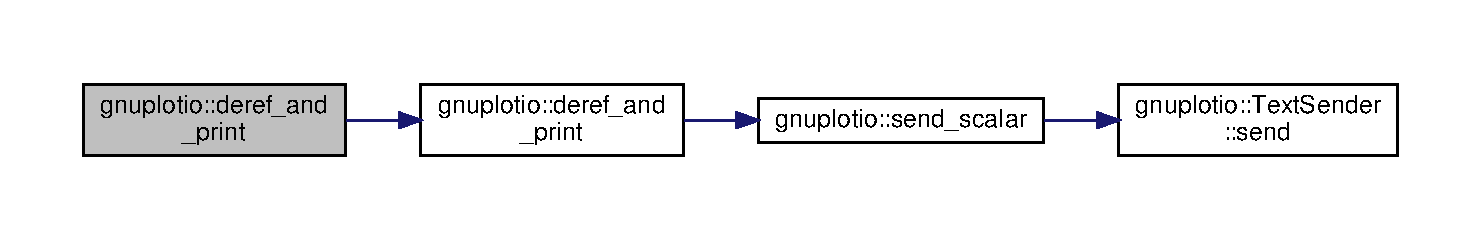
\includegraphics[width=350pt]{namespacegnuplotio_acd0cb4bd9679f0b75bac15c8afcc10e6_cgraph}
\end{center}
\end{figure}
\mbox{\Hypertarget{namespacegnuplotio_a66d64f716e539dc233f8183b4ce71c09}\label{namespacegnuplotio_a66d64f716e539dc233f8183b4ce71c09}} 
\index{gnuplotio@{gnuplotio}!deref\_and\_print@{deref\_and\_print}}
\index{deref\_and\_print@{deref\_and\_print}!gnuplotio@{gnuplotio}}
\doxysubsubsection{\texorpdfstring{deref\_and\_print()}{deref\_and\_print()}\hspace{0.1cm}{\footnotesize\ttfamily [2/4]}}
{\footnotesize\ttfamily template$<$typename T , typename Print\+Mode $>$ \\
boost\+::disable\+\_\+if\+\_\+c$<$T\+::is\+\_\+container$>$\+::type gnuplotio\+::deref\+\_\+and\+\_\+print (\begin{DoxyParamCaption}\item[{std\+::ostream \&}]{stream,  }\item[{const T \&}]{arg,  }\item[{Print\+Mode}]{ }\end{DoxyParamCaption})}



Definition at line 1317 of file gnuplot-\/iostream.\+h.



References send\+\_\+scalar().



Referenced by deref\+\_\+and\+\_\+print(), and print\+\_\+block().

Here is the call graph for this function\+:\nopagebreak
\begin{figure}[H]
\begin{center}
\leavevmode
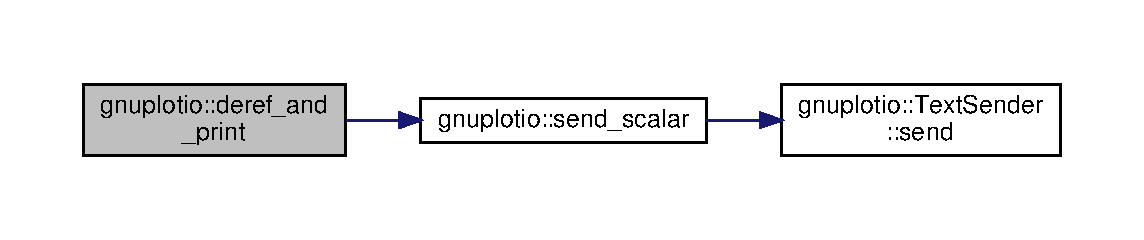
\includegraphics[width=350pt]{namespacegnuplotio_a66d64f716e539dc233f8183b4ce71c09_cgraph}
\end{center}
\end{figure}
\mbox{\Hypertarget{namespacegnuplotio_a8c6b699dd18c419d597a008b74eda41a}\label{namespacegnuplotio_a8c6b699dd18c419d597a008b74eda41a}} 
\index{gnuplotio@{gnuplotio}!deref\_and\_print@{deref\_and\_print}}
\index{deref\_and\_print@{deref\_and\_print}!gnuplotio@{gnuplotio}}
\doxysubsubsection{\texorpdfstring{deref\_and\_print()}{deref\_and\_print()}\hspace{0.1cm}{\footnotesize\ttfamily [3/4]}}
{\footnotesize\ttfamily template$<$typename T , typename Print\+Mode $>$ \\
boost\+::enable\+\_\+if\+\_\+c$<$T\+::is\+\_\+container$>$\+::type gnuplotio\+::deref\+\_\+and\+\_\+print (\begin{DoxyParamCaption}\item[{std\+::ostream \&}]{stream,  }\item[{const T \&}]{arg,  }\item[{Print\+Mode}]{ }\end{DoxyParamCaption})}



Definition at line 1327 of file gnuplot-\/iostream.\+h.



References deref\+\_\+and\+\_\+print().

Here is the call graph for this function\+:\nopagebreak
\begin{figure}[H]
\begin{center}
\leavevmode
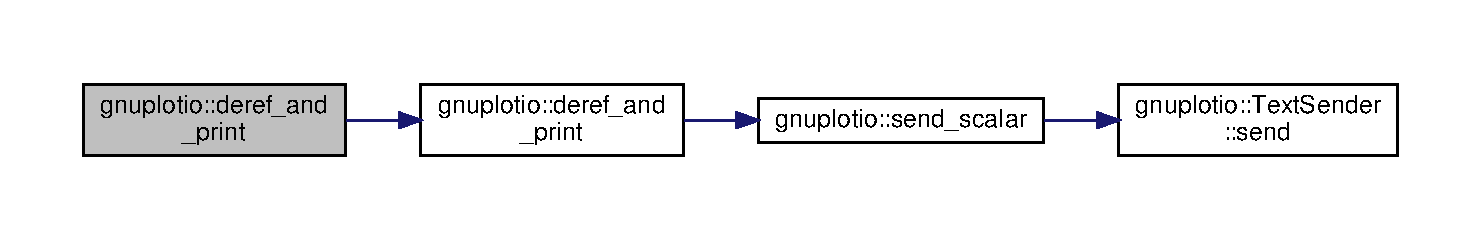
\includegraphics[width=350pt]{namespacegnuplotio_a8c6b699dd18c419d597a008b74eda41a_cgraph}
\end{center}
\end{figure}
\mbox{\Hypertarget{namespacegnuplotio_ae768911c8adb77bfc080d5e4561573e6}\label{namespacegnuplotio_ae768911c8adb77bfc080d5e4561573e6}} 
\index{gnuplotio@{gnuplotio}!deref\_and\_print@{deref\_and\_print}}
\index{deref\_and\_print@{deref\_and\_print}!gnuplotio@{gnuplotio}}
\doxysubsubsection{\texorpdfstring{deref\_and\_print()}{deref\_and\_print()}\hspace{0.1cm}{\footnotesize\ttfamily [4/4]}}
{\footnotesize\ttfamily template$<$typename T , typename Print\+Mode $>$ \\
void gnuplotio\+::deref\+\_\+and\+\_\+print (\begin{DoxyParamCaption}\item[{std\+::ostream \&}]{stream,  }\item[{const \mbox{\hyperlink{classgnuplotio_1_1_vec_of_range}{Vec\+Of\+Range}}$<$ T $>$ \&}]{arg,  }\item[{Print\+Mode}]{ }\end{DoxyParamCaption})}



Definition at line 1352 of file gnuplot-\/iostream.\+h.



References deref\+\_\+and\+\_\+print().

Here is the call graph for this function\+:\nopagebreak
\begin{figure}[H]
\begin{center}
\leavevmode
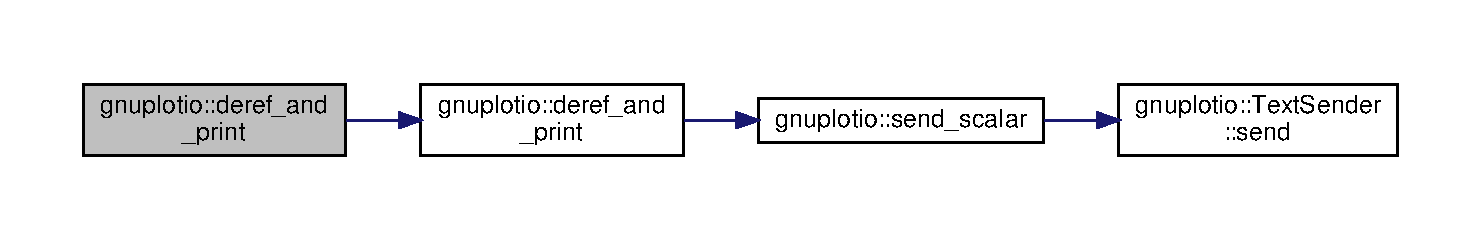
\includegraphics[width=350pt]{namespacegnuplotio_ae768911c8adb77bfc080d5e4561573e6_cgraph}
\end{center}
\end{figure}
\mbox{\Hypertarget{namespacegnuplotio_a64984827dd8debb9098ad1afdde8e409}\label{namespacegnuplotio_a64984827dd8debb9098ad1afdde8e409}} 
\index{gnuplotio@{gnuplotio}!get\_columns\_range@{get\_columns\_range}}
\index{get\_columns\_range@{get\_columns\_range}!gnuplotio@{gnuplotio}}
\doxysubsubsection{\texorpdfstring{get\_columns\_range()}{get\_columns\_range()}}
{\footnotesize\ttfamily template$<$typename T $>$ \\
\mbox{\hyperlink{classgnuplotio_1_1_vec_of_range}{Vec\+Of\+Range}}$<$typename \mbox{\hyperlink{classgnuplotio_1_1_array_traits}{Array\+Traits}}$<$T$>$\+::range\+\_\+type\+::subiter\+\_\+type$>$ gnuplotio\+::get\+\_\+columns\+\_\+range (\begin{DoxyParamCaption}\item[{const T \&}]{arg }\end{DoxyParamCaption})}



Definition at line 1150 of file gnuplot-\/iostream.\+h.



References gnuplotio\+::\+Array\+Traits$<$ T, Enable $>$\+::get\+\_\+range().



Referenced by handle\+\_\+colunwrap\+\_\+tag().

Here is the call graph for this function\+:\nopagebreak
\begin{figure}[H]
\begin{center}
\leavevmode
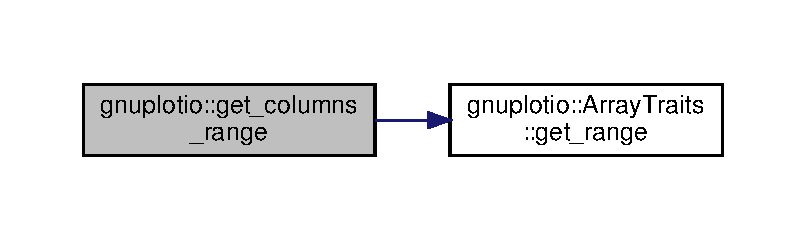
\includegraphics[width=350pt]{namespacegnuplotio_a64984827dd8debb9098ad1afdde8e409_cgraph}
\end{center}
\end{figure}
\mbox{\Hypertarget{namespacegnuplotio_abb416b68686102ba84a2cb53c96b64e9}\label{namespacegnuplotio_abb416b68686102ba84a2cb53c96b64e9}} 
\index{gnuplotio@{gnuplotio}!get\_range\_size@{get\_range\_size}}
\index{get\_range\_size@{get\_range\_size}!gnuplotio@{gnuplotio}}
\doxysubsubsection{\texorpdfstring{get\_range\_size()}{get\_range\_size()}}
{\footnotesize\ttfamily template$<$typename T $>$ \\
size\+\_\+t gnuplotio\+::get\+\_\+range\+\_\+size (\begin{DoxyParamCaption}\item[{const T \&}]{arg }\end{DoxyParamCaption})}



Definition at line 1418 of file gnuplot-\/iostream.\+h.



Referenced by print\+\_\+block().

\mbox{\Hypertarget{namespacegnuplotio_aef147f3d42f3f2c89cc4c895b8494150}\label{namespacegnuplotio_aef147f3d42f3f2c89cc4c895b8494150}} 
\index{gnuplotio@{gnuplotio}!handle\_colunwrap\_tag@{handle\_colunwrap\_tag}}
\index{handle\_colunwrap\_tag@{handle\_colunwrap\_tag}!gnuplotio@{gnuplotio}}
\doxysubsubsection{\texorpdfstring{handle\_colunwrap\_tag()}{handle\_colunwrap\_tag()}\hspace{0.1cm}{\footnotesize\ttfamily [1/2]}}
{\footnotesize\ttfamily template$<$size\+\_\+t Depth, typename T , typename Print\+Mode $>$ \\
void gnuplotio\+::handle\+\_\+colunwrap\+\_\+tag (\begin{DoxyParamCaption}\item[{std\+::ostream \&}]{stream,  }\item[{const T \&}]{arg,  }\item[{\mbox{\hyperlink{structgnuplotio_1_1_col_unwrap_no}{Col\+Unwrap\+No}}}]{,  }\item[{Print\+Mode}]{ }\end{DoxyParamCaption})}



Definition at line 1453 of file gnuplot-\/iostream.\+h.



References gnuplotio\+::\+Array\+Traits$<$ T, Enable $>$\+::get\+\_\+range(), and G\+N\+U\+P\+L\+O\+T\+\_\+\+S\+T\+A\+T\+I\+C\+\_\+\+A\+S\+S\+E\+R\+T\+\_\+\+M\+SG.

Here is the call graph for this function\+:\nopagebreak
\begin{figure}[H]
\begin{center}
\leavevmode
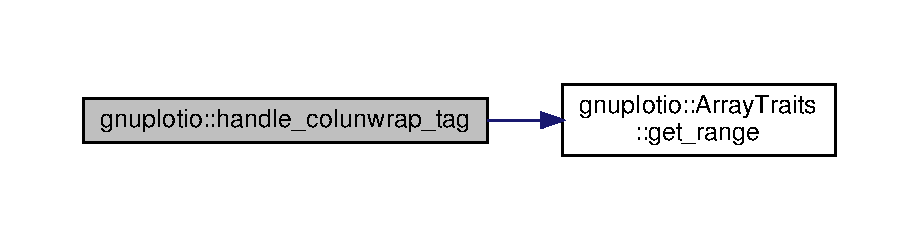
\includegraphics[width=350pt]{namespacegnuplotio_aef147f3d42f3f2c89cc4c895b8494150_cgraph}
\end{center}
\end{figure}
\mbox{\Hypertarget{namespacegnuplotio_a3b8981d3f39de8a058b5f18484f06c3c}\label{namespacegnuplotio_a3b8981d3f39de8a058b5f18484f06c3c}} 
\index{gnuplotio@{gnuplotio}!handle\_colunwrap\_tag@{handle\_colunwrap\_tag}}
\index{handle\_colunwrap\_tag@{handle\_colunwrap\_tag}!gnuplotio@{gnuplotio}}
\doxysubsubsection{\texorpdfstring{handle\_colunwrap\_tag()}{handle\_colunwrap\_tag()}\hspace{0.1cm}{\footnotesize\ttfamily [2/2]}}
{\footnotesize\ttfamily template$<$size\+\_\+t Depth, typename T , typename Print\+Mode $>$ \\
void gnuplotio\+::handle\+\_\+colunwrap\+\_\+tag (\begin{DoxyParamCaption}\item[{std\+::ostream \&}]{stream,  }\item[{const T \&}]{arg,  }\item[{\mbox{\hyperlink{structgnuplotio_1_1_col_unwrap_yes}{Col\+Unwrap\+Yes}}}]{,  }\item[{Print\+Mode}]{ }\end{DoxyParamCaption})}



Definition at line 1460 of file gnuplot-\/iostream.\+h.



References get\+\_\+columns\+\_\+range(), and G\+N\+U\+P\+L\+O\+T\+\_\+\+S\+T\+A\+T\+I\+C\+\_\+\+A\+S\+S\+E\+R\+T\+\_\+\+M\+SG.

Here is the call graph for this function\+:\nopagebreak
\begin{figure}[H]
\begin{center}
\leavevmode
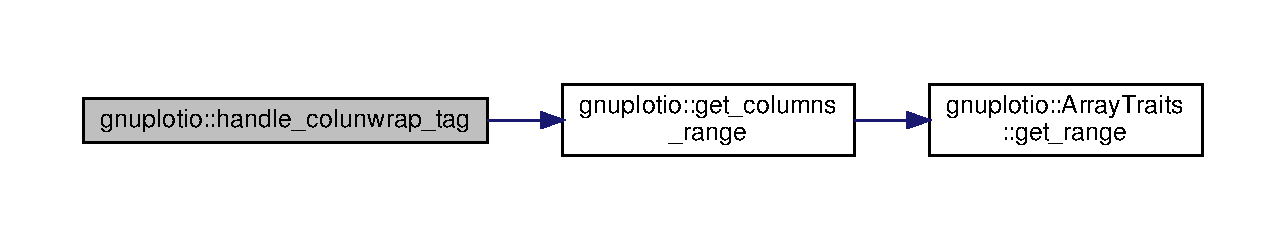
\includegraphics[width=350pt]{namespacegnuplotio_a3b8981d3f39de8a058b5f18484f06c3c_cgraph}
\end{center}
\end{figure}
\mbox{\Hypertarget{namespacegnuplotio_af809657552a53c3b17f0400a5c210a7f}\label{namespacegnuplotio_af809657552a53c3b17f0400a5c210a7f}} 
\index{gnuplotio@{gnuplotio}!handle\_organization\_tag@{handle\_organization\_tag}}
\index{handle\_organization\_tag@{handle\_organization\_tag}!gnuplotio@{gnuplotio}}
\doxysubsubsection{\texorpdfstring{handle\_organization\_tag()}{handle\_organization\_tag()}\hspace{0.1cm}{\footnotesize\ttfamily [1/5]}}
{\footnotesize\ttfamily template$<$typename T , typename Print\+Mode $>$ \\
void gnuplotio\+::handle\+\_\+organization\+\_\+tag (\begin{DoxyParamCaption}\item[{std\+::ostream \&}]{stream,  }\item[{const T \&}]{arg,  }\item[{\mbox{\hyperlink{structgnuplotio_1_1_mode1_d}{Mode1D}}}]{,  }\item[{Print\+Mode}]{ }\end{DoxyParamCaption})}



Definition at line 1476 of file gnuplot-\/iostream.\+h.



Referenced by handle\+\_\+organization\+\_\+tag(), and top\+\_\+level\+\_\+array\+\_\+sender().

\mbox{\Hypertarget{namespacegnuplotio_a99e6125b97bc2ca4241f6275d83f05d4}\label{namespacegnuplotio_a99e6125b97bc2ca4241f6275d83f05d4}} 
\index{gnuplotio@{gnuplotio}!handle\_organization\_tag@{handle\_organization\_tag}}
\index{handle\_organization\_tag@{handle\_organization\_tag}!gnuplotio@{gnuplotio}}
\doxysubsubsection{\texorpdfstring{handle\_organization\_tag()}{handle\_organization\_tag()}\hspace{0.1cm}{\footnotesize\ttfamily [2/5]}}
{\footnotesize\ttfamily template$<$typename T , typename Print\+Mode $>$ \\
void gnuplotio\+::handle\+\_\+organization\+\_\+tag (\begin{DoxyParamCaption}\item[{std\+::ostream \&}]{stream,  }\item[{const T \&}]{arg,  }\item[{\mbox{\hyperlink{structgnuplotio_1_1_mode1_d_unwrap}{Mode1\+D\+Unwrap}}}]{,  }\item[{Print\+Mode}]{ }\end{DoxyParamCaption})}



Definition at line 1486 of file gnuplot-\/iostream.\+h.

\mbox{\Hypertarget{namespacegnuplotio_a1310221abf0551a805d4482f0612317b}\label{namespacegnuplotio_a1310221abf0551a805d4482f0612317b}} 
\index{gnuplotio@{gnuplotio}!handle\_organization\_tag@{handle\_organization\_tag}}
\index{handle\_organization\_tag@{handle\_organization\_tag}!gnuplotio@{gnuplotio}}
\doxysubsubsection{\texorpdfstring{handle\_organization\_tag()}{handle\_organization\_tag()}\hspace{0.1cm}{\footnotesize\ttfamily [3/5]}}
{\footnotesize\ttfamily template$<$typename T , typename Print\+Mode $>$ \\
void gnuplotio\+::handle\+\_\+organization\+\_\+tag (\begin{DoxyParamCaption}\item[{std\+::ostream \&}]{stream,  }\item[{const T \&}]{arg,  }\item[{\mbox{\hyperlink{structgnuplotio_1_1_mode2_d}{Mode2D}}}]{,  }\item[{Print\+Mode}]{ }\end{DoxyParamCaption})}



Definition at line 1481 of file gnuplot-\/iostream.\+h.

\mbox{\Hypertarget{namespacegnuplotio_a9d2cee7a7f2ed9748a0f135b206836d3}\label{namespacegnuplotio_a9d2cee7a7f2ed9748a0f135b206836d3}} 
\index{gnuplotio@{gnuplotio}!handle\_organization\_tag@{handle\_organization\_tag}}
\index{handle\_organization\_tag@{handle\_organization\_tag}!gnuplotio@{gnuplotio}}
\doxysubsubsection{\texorpdfstring{handle\_organization\_tag()}{handle\_organization\_tag()}\hspace{0.1cm}{\footnotesize\ttfamily [4/5]}}
{\footnotesize\ttfamily template$<$typename T , typename Print\+Mode $>$ \\
void gnuplotio\+::handle\+\_\+organization\+\_\+tag (\begin{DoxyParamCaption}\item[{std\+::ostream \&}]{stream,  }\item[{const T \&}]{arg,  }\item[{\mbox{\hyperlink{structgnuplotio_1_1_mode2_d_unwrap}{Mode2\+D\+Unwrap}}}]{,  }\item[{Print\+Mode}]{ }\end{DoxyParamCaption})}



Definition at line 1491 of file gnuplot-\/iostream.\+h.

\mbox{\Hypertarget{namespacegnuplotio_affc9cb6a9b6e5630523f0dbf8acdfcc2}\label{namespacegnuplotio_affc9cb6a9b6e5630523f0dbf8acdfcc2}} 
\index{gnuplotio@{gnuplotio}!handle\_organization\_tag@{handle\_organization\_tag}}
\index{handle\_organization\_tag@{handle\_organization\_tag}!gnuplotio@{gnuplotio}}
\doxysubsubsection{\texorpdfstring{handle\_organization\_tag()}{handle\_organization\_tag()}\hspace{0.1cm}{\footnotesize\ttfamily [5/5]}}
{\footnotesize\ttfamily template$<$typename T , typename Print\+Mode $>$ \\
void gnuplotio\+::handle\+\_\+organization\+\_\+tag (\begin{DoxyParamCaption}\item[{std\+::ostream \&}]{stream,  }\item[{const T \&}]{arg,  }\item[{\mbox{\hyperlink{structgnuplotio_1_1_mode_auto}{Mode\+Auto}}}]{,  }\item[{Print\+Mode}]{ }\end{DoxyParamCaption})}



Definition at line 1496 of file gnuplot-\/iostream.\+h.



References handle\+\_\+organization\+\_\+tag().

Here is the call graph for this function\+:\nopagebreak
\begin{figure}[H]
\begin{center}
\leavevmode
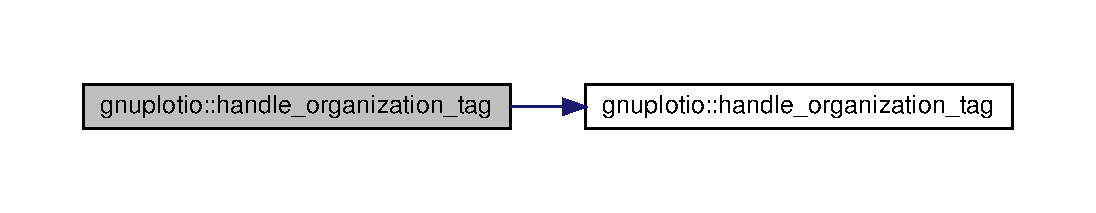
\includegraphics[width=350pt]{namespacegnuplotio_affc9cb6a9b6e5630523f0dbf8acdfcc2_cgraph}
\end{center}
\end{figure}
\mbox{\Hypertarget{namespacegnuplotio_a631368ab4e255d2a5d563a41895f2edc}\label{namespacegnuplotio_a631368ab4e255d2a5d563a41895f2edc}} 
\index{gnuplotio@{gnuplotio}!print\_block@{print\_block}}
\index{print\_block@{print\_block}!gnuplotio@{gnuplotio}}
\doxysubsubsection{\texorpdfstring{print\_block()}{print\_block()}\hspace{0.1cm}{\footnotesize\ttfamily [1/4]}}
{\footnotesize\ttfamily template$<$size\+\_\+t Depth, typename T , typename Print\+Mode $>$ \\
boost\+::enable\+\_\+if\+\_\+c$<$(Depth==1) \&\& !Print\+Mode\+::is\+\_\+size$>$\+::type gnuplotio\+::print\+\_\+block (\begin{DoxyParamCaption}\item[{std\+::ostream \&}]{stream,  }\item[{T \&}]{arg,  }\item[{Print\+Mode}]{ }\end{DoxyParamCaption})}



Definition at line 1381 of file gnuplot-\/iostream.\+h.



References deref\+\_\+and\+\_\+print().



Referenced by print\+\_\+block().

Here is the call graph for this function\+:\nopagebreak
\begin{figure}[H]
\begin{center}
\leavevmode
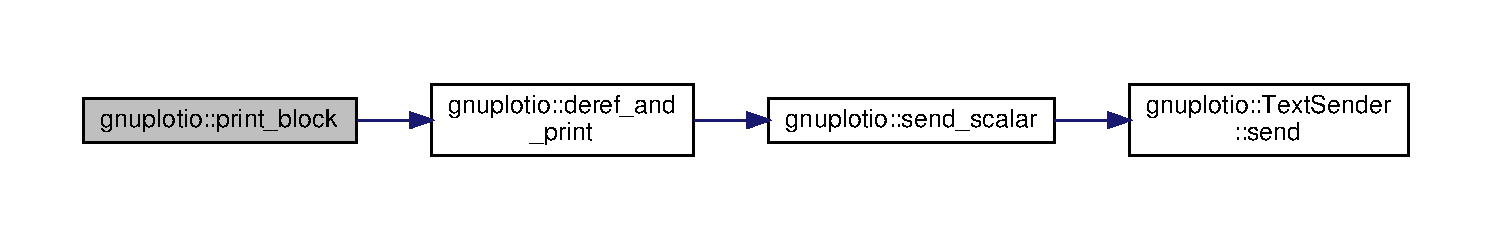
\includegraphics[width=350pt]{namespacegnuplotio_a631368ab4e255d2a5d563a41895f2edc_cgraph}
\end{center}
\end{figure}
\mbox{\Hypertarget{namespacegnuplotio_a753a3551f418723c022be60c12379025}\label{namespacegnuplotio_a753a3551f418723c022be60c12379025}} 
\index{gnuplotio@{gnuplotio}!print\_block@{print\_block}}
\index{print\_block@{print\_block}!gnuplotio@{gnuplotio}}
\doxysubsubsection{\texorpdfstring{print\_block()}{print\_block()}\hspace{0.1cm}{\footnotesize\ttfamily [2/4]}}
{\footnotesize\ttfamily template$<$size\+\_\+t Depth, typename T , typename Print\+Mode $>$ \\
boost\+::enable\+\_\+if\+\_\+c$<$(Depth$>$1) \&\& !Print\+Mode\+::is\+\_\+size$>$\+::type gnuplotio\+::print\+\_\+block (\begin{DoxyParamCaption}\item[{std\+::ostream \&}]{stream,  }\item[{T \&}]{arg,  }\item[{Print\+Mode}]{ }\end{DoxyParamCaption})}



Definition at line 1397 of file gnuplot-\/iostream.\+h.



References print\+\_\+block().

Here is the call graph for this function\+:\nopagebreak
\begin{figure}[H]
\begin{center}
\leavevmode
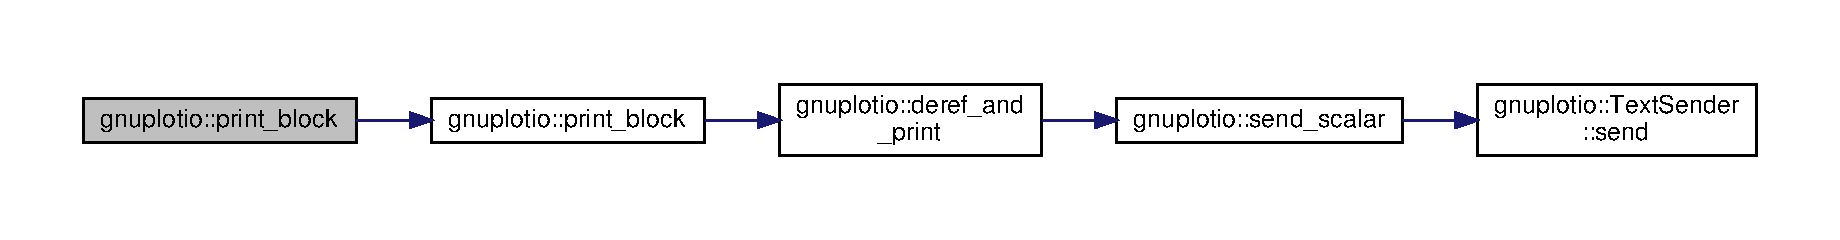
\includegraphics[width=350pt]{namespacegnuplotio_a753a3551f418723c022be60c12379025_cgraph}
\end{center}
\end{figure}
\mbox{\Hypertarget{namespacegnuplotio_ae470a0908ac5f51527ff76ecbc1616d1}\label{namespacegnuplotio_ae470a0908ac5f51527ff76ecbc1616d1}} 
\index{gnuplotio@{gnuplotio}!print\_block@{print\_block}}
\index{print\_block@{print\_block}!gnuplotio@{gnuplotio}}
\doxysubsubsection{\texorpdfstring{print\_block()}{print\_block()}\hspace{0.1cm}{\footnotesize\ttfamily [3/4]}}
{\footnotesize\ttfamily template$<$size\+\_\+t Depth, typename T , typename Print\+Mode $>$ \\
boost\+::enable\+\_\+if\+\_\+c$<$(Depth==1) \&\& Print\+Mode\+::is\+\_\+size$>$\+::type gnuplotio\+::print\+\_\+block (\begin{DoxyParamCaption}\item[{std\+::ostream \&}]{stream,  }\item[{T \&}]{arg,  }\item[{Print\+Mode}]{ }\end{DoxyParamCaption})}



Definition at line 1428 of file gnuplot-\/iostream.\+h.



References get\+\_\+range\+\_\+size().

Here is the call graph for this function\+:\nopagebreak
\begin{figure}[H]
\begin{center}
\leavevmode
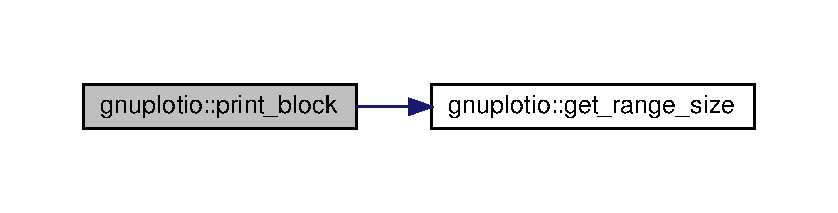
\includegraphics[width=350pt]{namespacegnuplotio_ae470a0908ac5f51527ff76ecbc1616d1_cgraph}
\end{center}
\end{figure}
\mbox{\Hypertarget{namespacegnuplotio_a94e97ca55dc1e5142dcc4457a5e1dd2d}\label{namespacegnuplotio_a94e97ca55dc1e5142dcc4457a5e1dd2d}} 
\index{gnuplotio@{gnuplotio}!print\_block@{print\_block}}
\index{print\_block@{print\_block}!gnuplotio@{gnuplotio}}
\doxysubsubsection{\texorpdfstring{print\_block()}{print\_block()}\hspace{0.1cm}{\footnotesize\ttfamily [4/4]}}
{\footnotesize\ttfamily template$<$size\+\_\+t Depth, typename T , typename Print\+Mode $>$ \\
boost\+::enable\+\_\+if\+\_\+c$<$(Depth$>$1) \&\& Print\+Mode\+::is\+\_\+size$>$\+::type gnuplotio\+::print\+\_\+block (\begin{DoxyParamCaption}\item[{std\+::ostream \&}]{stream,  }\item[{T \&}]{arg,  }\item[{Print\+Mode}]{ }\end{DoxyParamCaption})}



Definition at line 1435 of file gnuplot-\/iostream.\+h.



References get\+\_\+range\+\_\+size(), and print\+\_\+block().

Here is the call graph for this function\+:\nopagebreak
\begin{figure}[H]
\begin{center}
\leavevmode
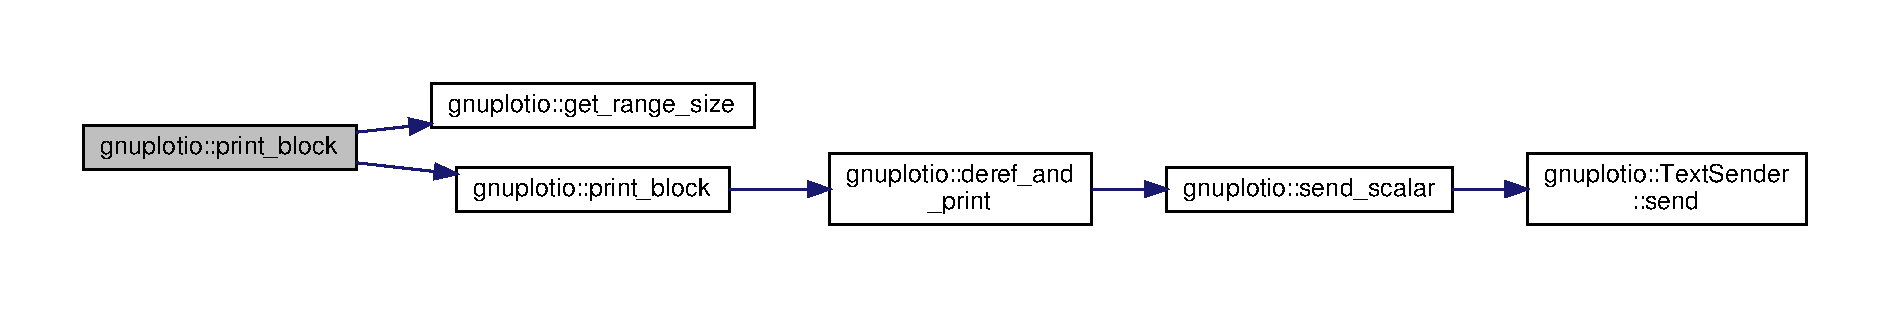
\includegraphics[width=350pt]{namespacegnuplotio_a94e97ca55dc1e5142dcc4457a5e1dd2d_cgraph}
\end{center}
\end{figure}
\mbox{\Hypertarget{namespacegnuplotio_a926e0935a02d83735da2c34cfbad133f}\label{namespacegnuplotio_a926e0935a02d83735da2c34cfbad133f}} 
\index{gnuplotio@{gnuplotio}!send\_scalar@{send\_scalar}}
\index{send\_scalar@{send\_scalar}!gnuplotio@{gnuplotio}}
\doxysubsubsection{\texorpdfstring{send\_scalar()}{send\_scalar()}\hspace{0.1cm}{\footnotesize\ttfamily [1/3]}}
{\footnotesize\ttfamily template$<$typename T $>$ \\
void gnuplotio\+::send\+\_\+scalar (\begin{DoxyParamCaption}\item[{std\+::ostream \&}]{stream,  }\item[{const T \&}]{,  }\item[{\mbox{\hyperlink{structgnuplotio_1_1_mode_binfmt}{Mode\+Binfmt}}}]{ }\end{DoxyParamCaption})}



Definition at line 1302 of file gnuplot-\/iostream.\+h.



References gnuplotio\+::\+Binfmt\+Sender$<$ T, Enable $>$\+::send().

Here is the call graph for this function\+:\nopagebreak
\begin{figure}[H]
\begin{center}
\leavevmode
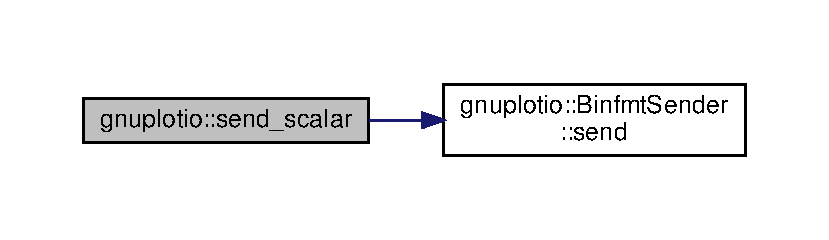
\includegraphics[width=350pt]{namespacegnuplotio_a926e0935a02d83735da2c34cfbad133f_cgraph}
\end{center}
\end{figure}
\mbox{\Hypertarget{namespacegnuplotio_a05022d6e136d8ed89a2bef0f61443332}\label{namespacegnuplotio_a05022d6e136d8ed89a2bef0f61443332}} 
\index{gnuplotio@{gnuplotio}!send\_scalar@{send\_scalar}}
\index{send\_scalar@{send\_scalar}!gnuplotio@{gnuplotio}}
\doxysubsubsection{\texorpdfstring{send\_scalar()}{send\_scalar()}\hspace{0.1cm}{\footnotesize\ttfamily [2/3]}}
{\footnotesize\ttfamily template$<$typename T $>$ \\
void gnuplotio\+::send\+\_\+scalar (\begin{DoxyParamCaption}\item[{std\+::ostream \&}]{stream,  }\item[{const T \&}]{arg,  }\item[{\mbox{\hyperlink{structgnuplotio_1_1_mode_binary}{Mode\+Binary}}}]{ }\end{DoxyParamCaption})}



Definition at line 1297 of file gnuplot-\/iostream.\+h.



References gnuplotio\+::\+Binary\+Sender$<$ T, Enable $>$\+::send().

Here is the call graph for this function\+:\nopagebreak
\begin{figure}[H]
\begin{center}
\leavevmode
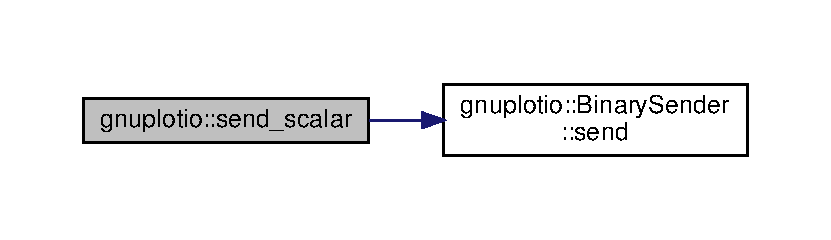
\includegraphics[width=350pt]{namespacegnuplotio_a05022d6e136d8ed89a2bef0f61443332_cgraph}
\end{center}
\end{figure}
\mbox{\Hypertarget{namespacegnuplotio_a55ff2f9abaa4b3e1c64a8f730f791b33}\label{namespacegnuplotio_a55ff2f9abaa4b3e1c64a8f730f791b33}} 
\index{gnuplotio@{gnuplotio}!send\_scalar@{send\_scalar}}
\index{send\_scalar@{send\_scalar}!gnuplotio@{gnuplotio}}
\doxysubsubsection{\texorpdfstring{send\_scalar()}{send\_scalar()}\hspace{0.1cm}{\footnotesize\ttfamily [3/3]}}
{\footnotesize\ttfamily template$<$typename T $>$ \\
void gnuplotio\+::send\+\_\+scalar (\begin{DoxyParamCaption}\item[{std\+::ostream \&}]{stream,  }\item[{const T \&}]{arg,  }\item[{\mbox{\hyperlink{structgnuplotio_1_1_mode_text}{Mode\+Text}}}]{ }\end{DoxyParamCaption})}



Definition at line 1292 of file gnuplot-\/iostream.\+h.



References gnuplotio\+::\+Text\+Sender$<$ T, Enable $>$\+::send().



Referenced by deref\+\_\+and\+\_\+print().

Here is the call graph for this function\+:\nopagebreak
\begin{figure}[H]
\begin{center}
\leavevmode
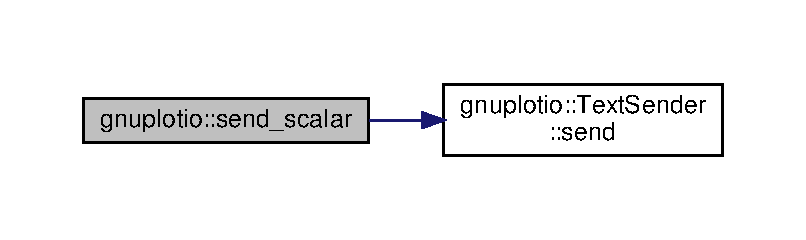
\includegraphics[width=350pt]{namespacegnuplotio_a55ff2f9abaa4b3e1c64a8f730f791b33_cgraph}
\end{center}
\end{figure}
\mbox{\Hypertarget{namespacegnuplotio_a1e452d861932700749421ce103ef8d48}\label{namespacegnuplotio_a1e452d861932700749421ce103ef8d48}} 
\index{gnuplotio@{gnuplotio}!top\_level\_array\_sender@{top\_level\_array\_sender}}
\index{top\_level\_array\_sender@{top\_level\_array\_sender}!gnuplotio@{gnuplotio}}
\doxysubsubsection{\texorpdfstring{top\_level\_array\_sender()}{top\_level\_array\_sender()}}
{\footnotesize\ttfamily template$<$typename T , typename Organization\+Mode , typename Print\+Mode $>$ \\
void gnuplotio\+::top\+\_\+level\+\_\+array\+\_\+sender (\begin{DoxyParamCaption}\item[{std\+::ostream \&}]{stream,  }\item[{const T \&}]{arg,  }\item[{Organization\+Mode}]{,  }\item[{Print\+Mode}]{ }\end{DoxyParamCaption})}



Definition at line 1509 of file gnuplot-\/iostream.\+h.



References handle\+\_\+organization\+\_\+tag().



Referenced by gnuplotio\+::\+Gnuplot\+::binary\+File(), gnuplotio\+::\+Gnuplot\+::binfmt(), gnuplotio\+::\+Gnuplot\+::file(), gnuplotio\+::\+Gnuplot\+::send(), and gnuplotio\+::\+Gnuplot\+::send\+Binary().

Here is the call graph for this function\+:\nopagebreak
\begin{figure}[H]
\begin{center}
\leavevmode
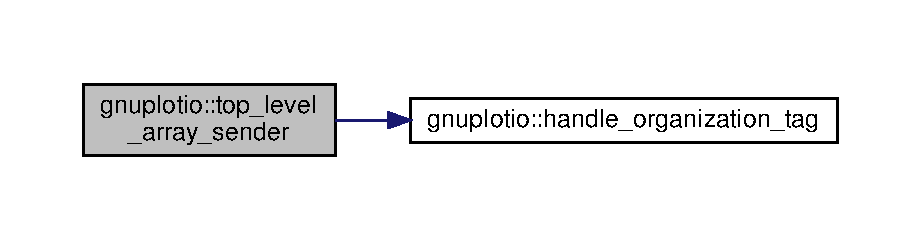
\includegraphics[width=350pt]{namespacegnuplotio_a1e452d861932700749421ce103ef8d48_cgraph}
\end{center}
\end{figure}

\hypertarget{namespacestp}{}\doxysection{stp Namespace Reference}
\label{namespacestp}\index{stp@{stp}}
\doxysubsection*{Classes}
\begin{DoxyCompactItemize}
\item 
class \mbox{\hyperlink{classstp_1_1_gazebo__sim}{Gazebo\+\_\+sim}}
\item 
class \mbox{\hyperlink{classstp_1_1_gnuplot__sim}{Gnuplot\+\_\+sim}}
\item 
class \mbox{\hyperlink{classstp_1_1_model}{Model}}
\item 
class \mbox{\hyperlink{classstp_1_1_platform}{Platform}}
\end{DoxyCompactItemize}

\chapter{Class Documentation}
\hypertarget{classgnuplotio_1_1_array_traits}{}\doxysection{gnuplotio\+::Array\+Traits$<$ T, Enable $>$ Class Template Reference}
\label{classgnuplotio_1_1_array_traits}\index{gnuplotio::ArrayTraits$<$ T, Enable $>$@{gnuplotio::ArrayTraits$<$ T, Enable $>$}}


{\ttfamily \#include $<$gnuplot-\/iostream.\+h$>$}



Inheritance diagram for gnuplotio\+::Array\+Traits$<$ T, Enable $>$\+:\nopagebreak
\begin{figure}[H]
\begin{center}
\leavevmode
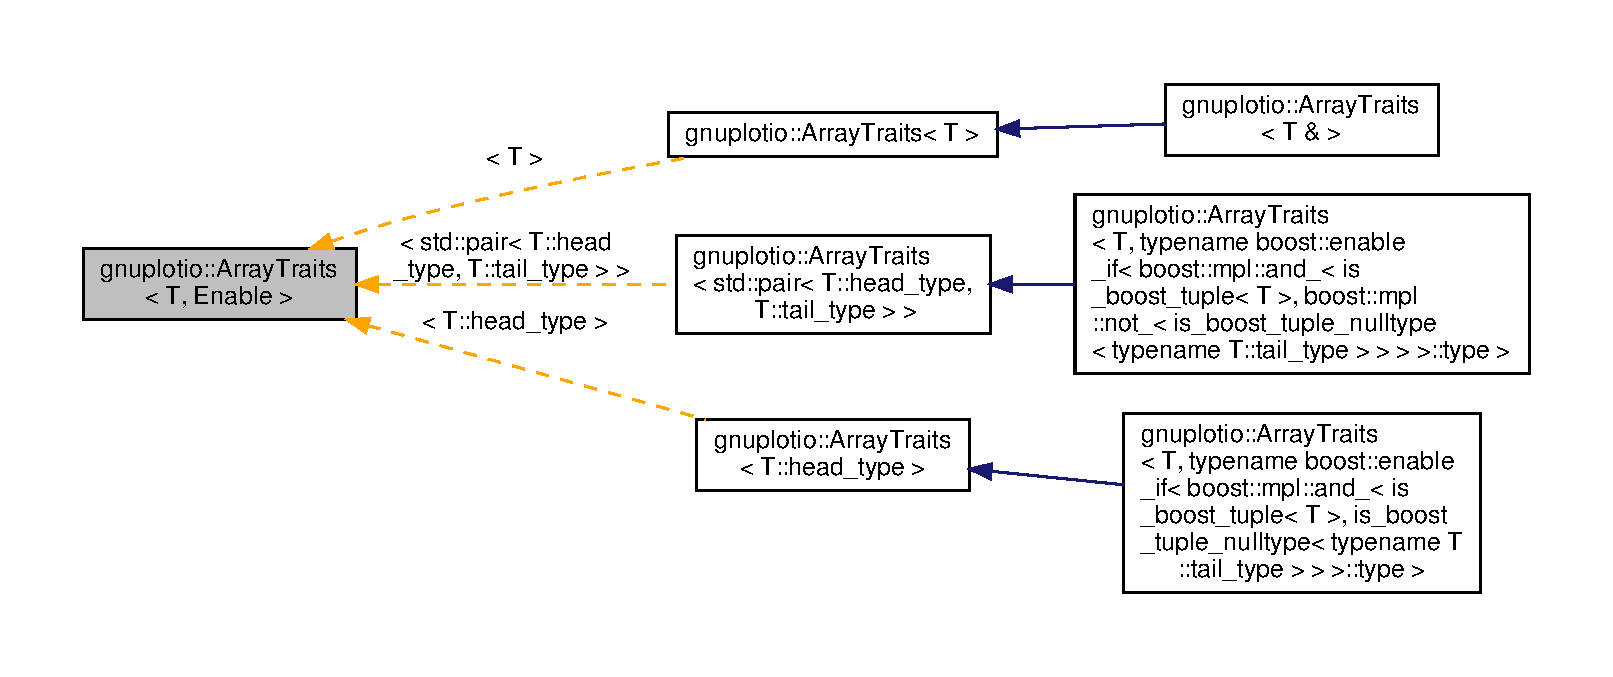
\includegraphics[width=350pt]{classgnuplotio_1_1_array_traits__inherit__graph}
\end{center}
\end{figure}
\doxysubsection*{Public Types}
\begin{DoxyCompactItemize}
\item 
typedef \mbox{\hyperlink{structgnuplotio_1_1_error___was_not_container}{Error\+\_\+\+Was\+Not\+Container}} \mbox{\hyperlink{classgnuplotio_1_1_array_traits_a3bcae12a7bf42af90f4946acc66f27e0}{value\+\_\+type}}
\item 
typedef \mbox{\hyperlink{structgnuplotio_1_1_error___was_not_container}{Error\+\_\+\+Was\+Not\+Container}} \mbox{\hyperlink{classgnuplotio_1_1_array_traits_ae53464a5175c03deec403392b8dcb3c5}{range\+\_\+type}}
\end{DoxyCompactItemize}
\doxysubsection*{Static Public Member Functions}
\begin{DoxyCompactItemize}
\item 
static \mbox{\hyperlink{classgnuplotio_1_1_array_traits_ae53464a5175c03deec403392b8dcb3c5}{range\+\_\+type}} \mbox{\hyperlink{classgnuplotio_1_1_array_traits_aee31432f330f9f9e4f5af628641181f7}{get\+\_\+range}} (const T \&)
\end{DoxyCompactItemize}
\doxysubsection*{Static Public Attributes}
\begin{DoxyCompactItemize}
\item 
static const bool \mbox{\hyperlink{classgnuplotio_1_1_array_traits_ac5d19b25086565613c305960bd9d4a78}{is\+\_\+container}} = false
\item 
static const bool \mbox{\hyperlink{classgnuplotio_1_1_array_traits_a354d64663551a34c36c5fa7823859668}{allow\+\_\+auto\+\_\+unwrap}} = false
\item 
static const size\+\_\+t \mbox{\hyperlink{classgnuplotio_1_1_array_traits_a6fbd8c815e595f4efbcafd9b0eeb06f2}{depth}} = 0
\end{DoxyCompactItemize}


\doxysubsection{Detailed Description}
\subsubsection*{template$<$typename T, typename Enable = void$>$\newline
class gnuplotio\+::\+Array\+Traits$<$ T, Enable $>$}



Definition at line 807 of file gnuplot-\/iostream.\+h.



\doxysubsection{Member Typedef Documentation}
\mbox{\Hypertarget{classgnuplotio_1_1_array_traits_ae53464a5175c03deec403392b8dcb3c5}\label{classgnuplotio_1_1_array_traits_ae53464a5175c03deec403392b8dcb3c5}} 
\index{gnuplotio::ArrayTraits$<$ T, Enable $>$@{gnuplotio::ArrayTraits$<$ T, Enable $>$}!range\_type@{range\_type}}
\index{range\_type@{range\_type}!gnuplotio::ArrayTraits$<$ T, Enable $>$@{gnuplotio::ArrayTraits$<$ T, Enable $>$}}
\doxysubsubsection{\texorpdfstring{range\_type}{range\_type}}
{\footnotesize\ttfamily template$<$typename T , typename Enable  = void$>$ \\
typedef \mbox{\hyperlink{structgnuplotio_1_1_error___was_not_container}{Error\+\_\+\+Was\+Not\+Container}} \mbox{\hyperlink{classgnuplotio_1_1_array_traits}{gnuplotio\+::\+Array\+Traits}}$<$ T, Enable $>$\+::\mbox{\hyperlink{classgnuplotio_1_1_array_traits_ae53464a5175c03deec403392b8dcb3c5}{range\+\_\+type}}}



Definition at line 812 of file gnuplot-\/iostream.\+h.

\mbox{\Hypertarget{classgnuplotio_1_1_array_traits_a3bcae12a7bf42af90f4946acc66f27e0}\label{classgnuplotio_1_1_array_traits_a3bcae12a7bf42af90f4946acc66f27e0}} 
\index{gnuplotio::ArrayTraits$<$ T, Enable $>$@{gnuplotio::ArrayTraits$<$ T, Enable $>$}!value\_type@{value\_type}}
\index{value\_type@{value\_type}!gnuplotio::ArrayTraits$<$ T, Enable $>$@{gnuplotio::ArrayTraits$<$ T, Enable $>$}}
\doxysubsubsection{\texorpdfstring{value\_type}{value\_type}}
{\footnotesize\ttfamily template$<$typename T , typename Enable  = void$>$ \\
typedef \mbox{\hyperlink{structgnuplotio_1_1_error___was_not_container}{Error\+\_\+\+Was\+Not\+Container}} \mbox{\hyperlink{classgnuplotio_1_1_array_traits}{gnuplotio\+::\+Array\+Traits}}$<$ T, Enable $>$\+::\mbox{\hyperlink{classgnuplotio_1_1_array_traits_a3bcae12a7bf42af90f4946acc66f27e0}{value\+\_\+type}}}



Definition at line 810 of file gnuplot-\/iostream.\+h.



\doxysubsection{Member Function Documentation}
\mbox{\Hypertarget{classgnuplotio_1_1_array_traits_aee31432f330f9f9e4f5af628641181f7}\label{classgnuplotio_1_1_array_traits_aee31432f330f9f9e4f5af628641181f7}} 
\index{gnuplotio::ArrayTraits$<$ T, Enable $>$@{gnuplotio::ArrayTraits$<$ T, Enable $>$}!get\_range@{get\_range}}
\index{get\_range@{get\_range}!gnuplotio::ArrayTraits$<$ T, Enable $>$@{gnuplotio::ArrayTraits$<$ T, Enable $>$}}
\doxysubsubsection{\texorpdfstring{get\_range()}{get\_range()}}
{\footnotesize\ttfamily template$<$typename T , typename Enable  = void$>$ \\
static \mbox{\hyperlink{classgnuplotio_1_1_array_traits_ae53464a5175c03deec403392b8dcb3c5}{range\+\_\+type}} \mbox{\hyperlink{classgnuplotio_1_1_array_traits}{gnuplotio\+::\+Array\+Traits}}$<$ T, Enable $>$\+::get\+\_\+range (\begin{DoxyParamCaption}\item[{const T \&}]{ }\end{DoxyParamCaption})\hspace{0.3cm}{\ttfamily [inline]}, {\ttfamily [static]}}



Definition at line 824 of file gnuplot-\/iostream.\+h.



Referenced by gnuplotio\+::\+Iterator\+Range$<$ T\+I, T\+V $>$\+::deref\+\_\+subiter(), gnuplotio\+::get\+\_\+columns\+\_\+range(), and gnuplotio\+::handle\+\_\+colunwrap\+\_\+tag().



\doxysubsection{Member Data Documentation}
\mbox{\Hypertarget{classgnuplotio_1_1_array_traits_a354d64663551a34c36c5fa7823859668}\label{classgnuplotio_1_1_array_traits_a354d64663551a34c36c5fa7823859668}} 
\index{gnuplotio::ArrayTraits$<$ T, Enable $>$@{gnuplotio::ArrayTraits$<$ T, Enable $>$}!allow\_auto\_unwrap@{allow\_auto\_unwrap}}
\index{allow\_auto\_unwrap@{allow\_auto\_unwrap}!gnuplotio::ArrayTraits$<$ T, Enable $>$@{gnuplotio::ArrayTraits$<$ T, Enable $>$}}
\doxysubsubsection{\texorpdfstring{allow\_auto\_unwrap}{allow\_auto\_unwrap}}
{\footnotesize\ttfamily template$<$typename T , typename Enable  = void$>$ \\
const bool \mbox{\hyperlink{classgnuplotio_1_1_array_traits}{gnuplotio\+::\+Array\+Traits}}$<$ T, Enable $>$\+::allow\+\_\+auto\+\_\+unwrap = false\hspace{0.3cm}{\ttfamily [static]}}



Definition at line 819 of file gnuplot-\/iostream.\+h.

\mbox{\Hypertarget{classgnuplotio_1_1_array_traits_a6fbd8c815e595f4efbcafd9b0eeb06f2}\label{classgnuplotio_1_1_array_traits_a6fbd8c815e595f4efbcafd9b0eeb06f2}} 
\index{gnuplotio::ArrayTraits$<$ T, Enable $>$@{gnuplotio::ArrayTraits$<$ T, Enable $>$}!depth@{depth}}
\index{depth@{depth}!gnuplotio::ArrayTraits$<$ T, Enable $>$@{gnuplotio::ArrayTraits$<$ T, Enable $>$}}
\doxysubsubsection{\texorpdfstring{depth}{depth}}
{\footnotesize\ttfamily template$<$typename T , typename Enable  = void$>$ \\
const size\+\_\+t \mbox{\hyperlink{classgnuplotio_1_1_array_traits}{gnuplotio\+::\+Array\+Traits}}$<$ T, Enable $>$\+::depth = 0\hspace{0.3cm}{\ttfamily [static]}}



Definition at line 821 of file gnuplot-\/iostream.\+h.

\mbox{\Hypertarget{classgnuplotio_1_1_array_traits_ac5d19b25086565613c305960bd9d4a78}\label{classgnuplotio_1_1_array_traits_ac5d19b25086565613c305960bd9d4a78}} 
\index{gnuplotio::ArrayTraits$<$ T, Enable $>$@{gnuplotio::ArrayTraits$<$ T, Enable $>$}!is\_container@{is\_container}}
\index{is\_container@{is\_container}!gnuplotio::ArrayTraits$<$ T, Enable $>$@{gnuplotio::ArrayTraits$<$ T, Enable $>$}}
\doxysubsubsection{\texorpdfstring{is\_container}{is\_container}}
{\footnotesize\ttfamily template$<$typename T , typename Enable  = void$>$ \\
const bool \mbox{\hyperlink{classgnuplotio_1_1_array_traits}{gnuplotio\+::\+Array\+Traits}}$<$ T, Enable $>$\+::is\+\_\+container = false\hspace{0.3cm}{\ttfamily [static]}}



Definition at line 814 of file gnuplot-\/iostream.\+h.



The documentation for this class was generated from the following file\+:\begin{DoxyCompactItemize}
\item 
/home/adev/\+Documents/\+S\+T\+E\+C\+H/stewart\+\_\+platform/include/\mbox{\hyperlink{gnuplot-iostream_8h}{gnuplot-\/iostream.\+h}}\end{DoxyCompactItemize}

\hypertarget{classgnuplotio_1_1_array_traits_3_01std_1_1pair_3_01_t_00_01_u_01_4_01_4}{}\section{gnuplotio\+:\+:Array\+Traits$<$ std\+:\+:pair$<$ T, U $>$ $>$ Class Template Reference}
\label{classgnuplotio_1_1_array_traits_3_01std_1_1pair_3_01_t_00_01_u_01_4_01_4}\index{gnuplotio\+::\+Array\+Traits$<$ std\+::pair$<$ T, U $>$ $>$@{gnuplotio\+::\+Array\+Traits$<$ std\+::pair$<$ T, U $>$ $>$}}


{\ttfamily \#include $<$gnuplot-\/iostream.\+h$>$}

\subsection*{Public Types}
\begin{DoxyCompactItemize}
\item 
typedef \hyperlink{classgnuplotio_1_1_pair_of_range}{Pair\+Of\+Range}$<$ typename \hyperlink{classgnuplotio_1_1_array_traits}{Array\+Traits}$<$ T $>$\+::\hyperlink{classgnuplotio_1_1_array_traits_3_01std_1_1pair_3_01_t_00_01_u_01_4_01_4_a80b3c6c794a51c78f0c645e5e4c19afc}{range\+\_\+type}, typename \hyperlink{classgnuplotio_1_1_array_traits}{Array\+Traits}$<$ U $>$\+::\hyperlink{classgnuplotio_1_1_array_traits_3_01std_1_1pair_3_01_t_00_01_u_01_4_01_4_a80b3c6c794a51c78f0c645e5e4c19afc}{range\+\_\+type} $>$ \hyperlink{classgnuplotio_1_1_array_traits_3_01std_1_1pair_3_01_t_00_01_u_01_4_01_4_a80b3c6c794a51c78f0c645e5e4c19afc}{range\+\_\+type}
\item 
typedef std\+::pair$<$ typename \hyperlink{classgnuplotio_1_1_array_traits}{Array\+Traits}$<$ T $>$\+::\hyperlink{classgnuplotio_1_1_array_traits_3_01std_1_1pair_3_01_t_00_01_u_01_4_01_4_a143ab4d4cf6693d33e46fa41d3265aab}{value\+\_\+type}, typename \hyperlink{classgnuplotio_1_1_array_traits}{Array\+Traits}$<$ U $>$\+::\hyperlink{classgnuplotio_1_1_array_traits_3_01std_1_1pair_3_01_t_00_01_u_01_4_01_4_a143ab4d4cf6693d33e46fa41d3265aab}{value\+\_\+type} $>$ \hyperlink{classgnuplotio_1_1_array_traits_3_01std_1_1pair_3_01_t_00_01_u_01_4_01_4_a143ab4d4cf6693d33e46fa41d3265aab}{value\+\_\+type}
\end{DoxyCompactItemize}
\subsection*{Static Public Member Functions}
\begin{DoxyCompactItemize}
\item 
static \hyperlink{classgnuplotio_1_1_array_traits_3_01std_1_1pair_3_01_t_00_01_u_01_4_01_4_a80b3c6c794a51c78f0c645e5e4c19afc}{range\+\_\+type} \hyperlink{classgnuplotio_1_1_array_traits_3_01std_1_1pair_3_01_t_00_01_u_01_4_01_4_abc84b60061de787f3526163183e186f7}{get\+\_\+range} (const std\+::pair$<$ T, U $>$ \&arg)
\end{DoxyCompactItemize}
\subsection*{Static Public Attributes}
\begin{DoxyCompactItemize}
\item 
static const bool \hyperlink{classgnuplotio_1_1_array_traits_3_01std_1_1pair_3_01_t_00_01_u_01_4_01_4_a8656ab8094037d88b470f718ff7197e0}{is\+\_\+container} = \hyperlink{classgnuplotio_1_1_array_traits}{Array\+Traits}$<$T$>$\+::is\+\_\+container \&\& \hyperlink{classgnuplotio_1_1_array_traits}{Array\+Traits}$<$U$>$\+::is\+\_\+container
\item 
static const bool \hyperlink{classgnuplotio_1_1_array_traits_3_01std_1_1pair_3_01_t_00_01_u_01_4_01_4_afff9ebffb39ab8660bb59ffcc7d8a2e5}{allow\+\_\+auto\+\_\+unwrap} = false
\item 
static const size\+\_\+t \hyperlink{classgnuplotio_1_1_array_traits_3_01std_1_1pair_3_01_t_00_01_u_01_4_01_4_ae8be9661c88a8970da3d87c1afc063dc}{l\+\_\+depth} = \hyperlink{classgnuplotio_1_1_array_traits}{Array\+Traits}$<$T$>$\+::\hyperlink{classgnuplotio_1_1_array_traits_3_01std_1_1pair_3_01_t_00_01_u_01_4_01_4_a11b3be89ac9506fcfcceb318acc7e2bf}{depth}
\item 
static const size\+\_\+t \hyperlink{classgnuplotio_1_1_array_traits_3_01std_1_1pair_3_01_t_00_01_u_01_4_01_4_a1b7e7f8976a5d0ed20b93ede3e25a546}{r\+\_\+depth} = \hyperlink{classgnuplotio_1_1_array_traits}{Array\+Traits}$<$U$>$\+::\hyperlink{classgnuplotio_1_1_array_traits_3_01std_1_1pair_3_01_t_00_01_u_01_4_01_4_a11b3be89ac9506fcfcceb318acc7e2bf}{depth}
\item 
static const size\+\_\+t \hyperlink{classgnuplotio_1_1_array_traits_3_01std_1_1pair_3_01_t_00_01_u_01_4_01_4_a11b3be89ac9506fcfcceb318acc7e2bf}{depth} = (\hyperlink{classgnuplotio_1_1_array_traits_3_01std_1_1pair_3_01_t_00_01_u_01_4_01_4_ae8be9661c88a8970da3d87c1afc063dc}{l\+\_\+depth} $<$ \hyperlink{classgnuplotio_1_1_array_traits_3_01std_1_1pair_3_01_t_00_01_u_01_4_01_4_a1b7e7f8976a5d0ed20b93ede3e25a546}{r\+\_\+depth}) ? \hyperlink{classgnuplotio_1_1_array_traits_3_01std_1_1pair_3_01_t_00_01_u_01_4_01_4_ae8be9661c88a8970da3d87c1afc063dc}{l\+\_\+depth} \+: \hyperlink{classgnuplotio_1_1_array_traits_3_01std_1_1pair_3_01_t_00_01_u_01_4_01_4_a1b7e7f8976a5d0ed20b93ede3e25a546}{r\+\_\+depth}
\end{DoxyCompactItemize}


\subsection{Detailed Description}
\subsubsection*{template$<$typename T, typename U$>$\newline
class gnuplotio\+::\+Array\+Traits$<$ std\+::pair$<$ T, U $>$ $>$}



Definition at line 968 of file gnuplot-\/iostream.\+h.



\subsection{Member Typedef Documentation}
\mbox{\Hypertarget{classgnuplotio_1_1_array_traits_3_01std_1_1pair_3_01_t_00_01_u_01_4_01_4_a80b3c6c794a51c78f0c645e5e4c19afc}\label{classgnuplotio_1_1_array_traits_3_01std_1_1pair_3_01_t_00_01_u_01_4_01_4_a80b3c6c794a51c78f0c645e5e4c19afc}} 
\index{gnuplotio\+::\+Array\+Traits$<$ std\+::pair$<$ T, U $>$ $>$@{gnuplotio\+::\+Array\+Traits$<$ std\+::pair$<$ T, U $>$ $>$}!range\+\_\+type@{range\+\_\+type}}
\index{range\+\_\+type@{range\+\_\+type}!gnuplotio\+::\+Array\+Traits$<$ std\+::pair$<$ T, U $>$ $>$@{gnuplotio\+::\+Array\+Traits$<$ std\+::pair$<$ T, U $>$ $>$}}
\subsubsection{\texorpdfstring{range\+\_\+type}{range\_type}}
{\footnotesize\ttfamily template$<$typename T , typename U $>$ \\
typedef \hyperlink{classgnuplotio_1_1_pair_of_range}{Pair\+Of\+Range}$<$typename \hyperlink{classgnuplotio_1_1_array_traits}{Array\+Traits}$<$T$>$\+::\hyperlink{classgnuplotio_1_1_array_traits_3_01std_1_1pair_3_01_t_00_01_u_01_4_01_4_a80b3c6c794a51c78f0c645e5e4c19afc}{range\+\_\+type}, typename \hyperlink{classgnuplotio_1_1_array_traits}{Array\+Traits}$<$U$>$\+::\hyperlink{classgnuplotio_1_1_array_traits_3_01std_1_1pair_3_01_t_00_01_u_01_4_01_4_a80b3c6c794a51c78f0c645e5e4c19afc}{range\+\_\+type}$>$ \hyperlink{classgnuplotio_1_1_array_traits}{gnuplotio\+::\+Array\+Traits}$<$ std\+::pair$<$ T, U $>$ $>$\+::\hyperlink{classgnuplotio_1_1_array_traits_3_01std_1_1pair_3_01_t_00_01_u_01_4_01_4_a80b3c6c794a51c78f0c645e5e4c19afc}{range\+\_\+type}}



Definition at line 970 of file gnuplot-\/iostream.\+h.

\mbox{\Hypertarget{classgnuplotio_1_1_array_traits_3_01std_1_1pair_3_01_t_00_01_u_01_4_01_4_a143ab4d4cf6693d33e46fa41d3265aab}\label{classgnuplotio_1_1_array_traits_3_01std_1_1pair_3_01_t_00_01_u_01_4_01_4_a143ab4d4cf6693d33e46fa41d3265aab}} 
\index{gnuplotio\+::\+Array\+Traits$<$ std\+::pair$<$ T, U $>$ $>$@{gnuplotio\+::\+Array\+Traits$<$ std\+::pair$<$ T, U $>$ $>$}!value\+\_\+type@{value\+\_\+type}}
\index{value\+\_\+type@{value\+\_\+type}!gnuplotio\+::\+Array\+Traits$<$ std\+::pair$<$ T, U $>$ $>$@{gnuplotio\+::\+Array\+Traits$<$ std\+::pair$<$ T, U $>$ $>$}}
\subsubsection{\texorpdfstring{value\+\_\+type}{value\_type}}
{\footnotesize\ttfamily template$<$typename T , typename U $>$ \\
typedef std\+::pair$<$typename \hyperlink{classgnuplotio_1_1_array_traits}{Array\+Traits}$<$T$>$\+::\hyperlink{classgnuplotio_1_1_array_traits_3_01std_1_1pair_3_01_t_00_01_u_01_4_01_4_a143ab4d4cf6693d33e46fa41d3265aab}{value\+\_\+type}, typename \hyperlink{classgnuplotio_1_1_array_traits}{Array\+Traits}$<$U$>$\+::\hyperlink{classgnuplotio_1_1_array_traits_3_01std_1_1pair_3_01_t_00_01_u_01_4_01_4_a143ab4d4cf6693d33e46fa41d3265aab}{value\+\_\+type}$>$ \hyperlink{classgnuplotio_1_1_array_traits}{gnuplotio\+::\+Array\+Traits}$<$ std\+::pair$<$ T, U $>$ $>$\+::\hyperlink{classgnuplotio_1_1_array_traits_3_01std_1_1pair_3_01_t_00_01_u_01_4_01_4_a143ab4d4cf6693d33e46fa41d3265aab}{value\+\_\+type}}



Definition at line 971 of file gnuplot-\/iostream.\+h.



\subsection{Member Function Documentation}
\mbox{\Hypertarget{classgnuplotio_1_1_array_traits_3_01std_1_1pair_3_01_t_00_01_u_01_4_01_4_abc84b60061de787f3526163183e186f7}\label{classgnuplotio_1_1_array_traits_3_01std_1_1pair_3_01_t_00_01_u_01_4_01_4_abc84b60061de787f3526163183e186f7}} 
\index{gnuplotio\+::\+Array\+Traits$<$ std\+::pair$<$ T, U $>$ $>$@{gnuplotio\+::\+Array\+Traits$<$ std\+::pair$<$ T, U $>$ $>$}!get\+\_\+range@{get\+\_\+range}}
\index{get\+\_\+range@{get\+\_\+range}!gnuplotio\+::\+Array\+Traits$<$ std\+::pair$<$ T, U $>$ $>$@{gnuplotio\+::\+Array\+Traits$<$ std\+::pair$<$ T, U $>$ $>$}}
\subsubsection{\texorpdfstring{get\+\_\+range()}{get\_range()}}
{\footnotesize\ttfamily template$<$typename T , typename U $>$ \\
static \hyperlink{classgnuplotio_1_1_array_traits_3_01std_1_1pair_3_01_t_00_01_u_01_4_01_4_a80b3c6c794a51c78f0c645e5e4c19afc}{range\+\_\+type} \hyperlink{classgnuplotio_1_1_array_traits}{gnuplotio\+::\+Array\+Traits}$<$ std\+::pair$<$ T, U $>$ $>$\+::get\+\_\+range (\begin{DoxyParamCaption}\item[{const std\+::pair$<$ T, U $>$ \&}]{arg }\end{DoxyParamCaption})\hspace{0.3cm}{\ttfamily [inline]}, {\ttfamily [static]}}



Definition at line 981 of file gnuplot-\/iostream.\+h.



\subsection{Member Data Documentation}
\mbox{\Hypertarget{classgnuplotio_1_1_array_traits_3_01std_1_1pair_3_01_t_00_01_u_01_4_01_4_afff9ebffb39ab8660bb59ffcc7d8a2e5}\label{classgnuplotio_1_1_array_traits_3_01std_1_1pair_3_01_t_00_01_u_01_4_01_4_afff9ebffb39ab8660bb59ffcc7d8a2e5}} 
\index{gnuplotio\+::\+Array\+Traits$<$ std\+::pair$<$ T, U $>$ $>$@{gnuplotio\+::\+Array\+Traits$<$ std\+::pair$<$ T, U $>$ $>$}!allow\+\_\+auto\+\_\+unwrap@{allow\+\_\+auto\+\_\+unwrap}}
\index{allow\+\_\+auto\+\_\+unwrap@{allow\+\_\+auto\+\_\+unwrap}!gnuplotio\+::\+Array\+Traits$<$ std\+::pair$<$ T, U $>$ $>$@{gnuplotio\+::\+Array\+Traits$<$ std\+::pair$<$ T, U $>$ $>$}}
\subsubsection{\texorpdfstring{allow\+\_\+auto\+\_\+unwrap}{allow\_auto\_unwrap}}
{\footnotesize\ttfamily template$<$typename T , typename U $>$ \\
const bool \hyperlink{classgnuplotio_1_1_array_traits}{gnuplotio\+::\+Array\+Traits}$<$ std\+::pair$<$ T, U $>$ $>$\+::allow\+\_\+auto\+\_\+unwrap = false\hspace{0.3cm}{\ttfamily [static]}}



Definition at line 974 of file gnuplot-\/iostream.\+h.

\mbox{\Hypertarget{classgnuplotio_1_1_array_traits_3_01std_1_1pair_3_01_t_00_01_u_01_4_01_4_a11b3be89ac9506fcfcceb318acc7e2bf}\label{classgnuplotio_1_1_array_traits_3_01std_1_1pair_3_01_t_00_01_u_01_4_01_4_a11b3be89ac9506fcfcceb318acc7e2bf}} 
\index{gnuplotio\+::\+Array\+Traits$<$ std\+::pair$<$ T, U $>$ $>$@{gnuplotio\+::\+Array\+Traits$<$ std\+::pair$<$ T, U $>$ $>$}!depth@{depth}}
\index{depth@{depth}!gnuplotio\+::\+Array\+Traits$<$ std\+::pair$<$ T, U $>$ $>$@{gnuplotio\+::\+Array\+Traits$<$ std\+::pair$<$ T, U $>$ $>$}}
\subsubsection{\texorpdfstring{depth}{depth}}
{\footnotesize\ttfamily template$<$typename T , typename U $>$ \\
const size\+\_\+t \hyperlink{classgnuplotio_1_1_array_traits}{gnuplotio\+::\+Array\+Traits}$<$ std\+::pair$<$ T, U $>$ $>$\+::depth = (\hyperlink{classgnuplotio_1_1_array_traits_3_01std_1_1pair_3_01_t_00_01_u_01_4_01_4_ae8be9661c88a8970da3d87c1afc063dc}{l\+\_\+depth} $<$ \hyperlink{classgnuplotio_1_1_array_traits_3_01std_1_1pair_3_01_t_00_01_u_01_4_01_4_a1b7e7f8976a5d0ed20b93ede3e25a546}{r\+\_\+depth}) ? \hyperlink{classgnuplotio_1_1_array_traits_3_01std_1_1pair_3_01_t_00_01_u_01_4_01_4_ae8be9661c88a8970da3d87c1afc063dc}{l\+\_\+depth} \+: \hyperlink{classgnuplotio_1_1_array_traits_3_01std_1_1pair_3_01_t_00_01_u_01_4_01_4_a1b7e7f8976a5d0ed20b93ede3e25a546}{r\+\_\+depth}\hspace{0.3cm}{\ttfamily [static]}}



Definition at line 979 of file gnuplot-\/iostream.\+h.

\mbox{\Hypertarget{classgnuplotio_1_1_array_traits_3_01std_1_1pair_3_01_t_00_01_u_01_4_01_4_a8656ab8094037d88b470f718ff7197e0}\label{classgnuplotio_1_1_array_traits_3_01std_1_1pair_3_01_t_00_01_u_01_4_01_4_a8656ab8094037d88b470f718ff7197e0}} 
\index{gnuplotio\+::\+Array\+Traits$<$ std\+::pair$<$ T, U $>$ $>$@{gnuplotio\+::\+Array\+Traits$<$ std\+::pair$<$ T, U $>$ $>$}!is\+\_\+container@{is\+\_\+container}}
\index{is\+\_\+container@{is\+\_\+container}!gnuplotio\+::\+Array\+Traits$<$ std\+::pair$<$ T, U $>$ $>$@{gnuplotio\+::\+Array\+Traits$<$ std\+::pair$<$ T, U $>$ $>$}}
\subsubsection{\texorpdfstring{is\+\_\+container}{is\_container}}
{\footnotesize\ttfamily template$<$typename T , typename U $>$ \\
const bool \hyperlink{classgnuplotio_1_1_array_traits}{gnuplotio\+::\+Array\+Traits}$<$ std\+::pair$<$ T, U $>$ $>$\+::is\+\_\+container = \hyperlink{classgnuplotio_1_1_array_traits}{Array\+Traits}$<$T$>$\+::is\+\_\+container \&\& \hyperlink{classgnuplotio_1_1_array_traits}{Array\+Traits}$<$U$>$\+::is\+\_\+container\hspace{0.3cm}{\ttfamily [static]}}



Definition at line 972 of file gnuplot-\/iostream.\+h.

\mbox{\Hypertarget{classgnuplotio_1_1_array_traits_3_01std_1_1pair_3_01_t_00_01_u_01_4_01_4_ae8be9661c88a8970da3d87c1afc063dc}\label{classgnuplotio_1_1_array_traits_3_01std_1_1pair_3_01_t_00_01_u_01_4_01_4_ae8be9661c88a8970da3d87c1afc063dc}} 
\index{gnuplotio\+::\+Array\+Traits$<$ std\+::pair$<$ T, U $>$ $>$@{gnuplotio\+::\+Array\+Traits$<$ std\+::pair$<$ T, U $>$ $>$}!l\+\_\+depth@{l\+\_\+depth}}
\index{l\+\_\+depth@{l\+\_\+depth}!gnuplotio\+::\+Array\+Traits$<$ std\+::pair$<$ T, U $>$ $>$@{gnuplotio\+::\+Array\+Traits$<$ std\+::pair$<$ T, U $>$ $>$}}
\subsubsection{\texorpdfstring{l\+\_\+depth}{l\_depth}}
{\footnotesize\ttfamily template$<$typename T , typename U $>$ \\
const size\+\_\+t \hyperlink{classgnuplotio_1_1_array_traits}{gnuplotio\+::\+Array\+Traits}$<$ std\+::pair$<$ T, U $>$ $>$\+::l\+\_\+depth = \hyperlink{classgnuplotio_1_1_array_traits}{Array\+Traits}$<$T$>$\+::\hyperlink{classgnuplotio_1_1_array_traits_3_01std_1_1pair_3_01_t_00_01_u_01_4_01_4_a11b3be89ac9506fcfcceb318acc7e2bf}{depth}\hspace{0.3cm}{\ttfamily [static]}}



Definition at line 977 of file gnuplot-\/iostream.\+h.

\mbox{\Hypertarget{classgnuplotio_1_1_array_traits_3_01std_1_1pair_3_01_t_00_01_u_01_4_01_4_a1b7e7f8976a5d0ed20b93ede3e25a546}\label{classgnuplotio_1_1_array_traits_3_01std_1_1pair_3_01_t_00_01_u_01_4_01_4_a1b7e7f8976a5d0ed20b93ede3e25a546}} 
\index{gnuplotio\+::\+Array\+Traits$<$ std\+::pair$<$ T, U $>$ $>$@{gnuplotio\+::\+Array\+Traits$<$ std\+::pair$<$ T, U $>$ $>$}!r\+\_\+depth@{r\+\_\+depth}}
\index{r\+\_\+depth@{r\+\_\+depth}!gnuplotio\+::\+Array\+Traits$<$ std\+::pair$<$ T, U $>$ $>$@{gnuplotio\+::\+Array\+Traits$<$ std\+::pair$<$ T, U $>$ $>$}}
\subsubsection{\texorpdfstring{r\+\_\+depth}{r\_depth}}
{\footnotesize\ttfamily template$<$typename T , typename U $>$ \\
const size\+\_\+t \hyperlink{classgnuplotio_1_1_array_traits}{gnuplotio\+::\+Array\+Traits}$<$ std\+::pair$<$ T, U $>$ $>$\+::r\+\_\+depth = \hyperlink{classgnuplotio_1_1_array_traits}{Array\+Traits}$<$U$>$\+::\hyperlink{classgnuplotio_1_1_array_traits_3_01std_1_1pair_3_01_t_00_01_u_01_4_01_4_a11b3be89ac9506fcfcceb318acc7e2bf}{depth}\hspace{0.3cm}{\ttfamily [static]}}



Definition at line 978 of file gnuplot-\/iostream.\+h.



The documentation for this class was generated from the following file\+:\begin{DoxyCompactItemize}
\item 
include/\hyperlink{gnuplot-iostream_8h}{gnuplot-\/iostream.\+h}\end{DoxyCompactItemize}

\hypertarget{classgnuplotio_1_1_array_traits_3_01_t_01_6_01_4}{}\doxysection{gnuplotio\+::Array\+Traits$<$ T \& $>$ Class Template Reference}
\label{classgnuplotio_1_1_array_traits_3_01_t_01_6_01_4}\index{gnuplotio::ArrayTraits$<$ T \& $>$@{gnuplotio::ArrayTraits$<$ T \& $>$}}


{\ttfamily \#include $<$gnuplot-\/iostream.\+h$>$}



Inheritance diagram for gnuplotio\+::Array\+Traits$<$ T \& $>$\+:\nopagebreak
\begin{figure}[H]
\begin{center}
\leavevmode
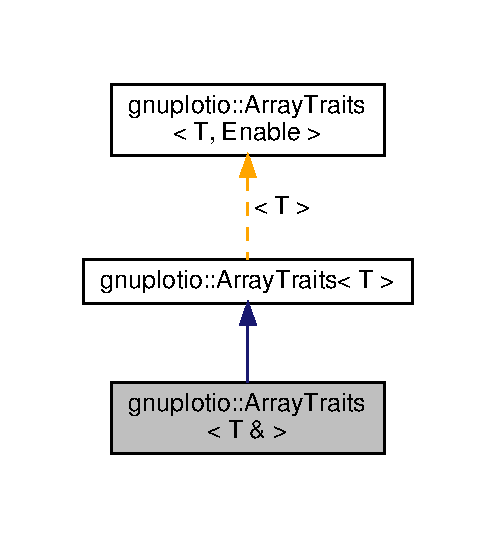
\includegraphics[width=257pt]{classgnuplotio_1_1_array_traits_3_01_t_01_6_01_4__inherit__graph}
\end{center}
\end{figure}


Collaboration diagram for gnuplotio\+::Array\+Traits$<$ T \& $>$\+:\nopagebreak
\begin{figure}[H]
\begin{center}
\leavevmode
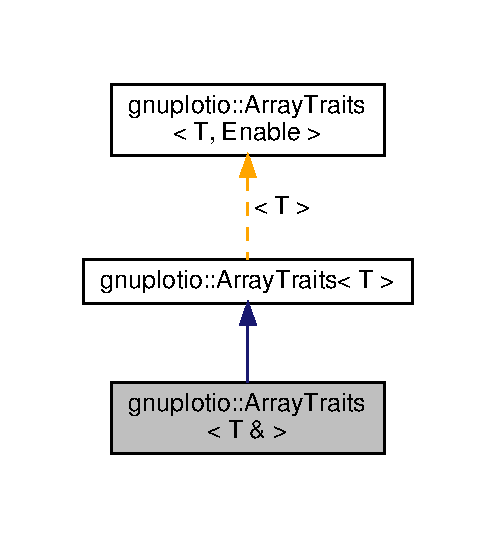
\includegraphics[width=257pt]{classgnuplotio_1_1_array_traits_3_01_t_01_6_01_4__coll__graph}
\end{center}
\end{figure}
\doxysubsection*{Additional Inherited Members}


\doxysubsection{Detailed Description}
\subsubsection*{template$<$typename T$>$\newline
class gnuplotio\+::\+Array\+Traits$<$ T \& $>$}



Definition at line 846 of file gnuplot-\/iostream.\+h.



The documentation for this class was generated from the following file\+:\begin{DoxyCompactItemize}
\item 
/home/adev/\+Documents/\+S\+T\+E\+C\+H/stewart\+\_\+platform/include/\mbox{\hyperlink{gnuplot-iostream_8h}{gnuplot-\/iostream.\+h}}\end{DoxyCompactItemize}

\hypertarget{classgnuplotio_1_1_array_traits_3_01_t_00_01typename_01boost_1_1enable__if_3_01boost_1_1mpl_1_1a8de3a8fe198d85f7f5d28b9a2f5bf229}{}\section{gnuplotio\+:\+:Array\+Traits$<$ T, typename boost\+:\+:enable\+\_\+if$<$ boost\+:\+:mpl\+:\+:and\+\_\+$<$ is\+\_\+boost\+\_\+tuple$<$ T $>$, boost\+:\+:mpl\+:\+:not\+\_\+$<$ is\+\_\+boost\+\_\+tuple\+\_\+nulltype$<$ typename T\+:\+:tail\+\_\+type $>$ $>$ $>$ $>$\+:\+:type $>$ Class Template Reference}
\label{classgnuplotio_1_1_array_traits_3_01_t_00_01typename_01boost_1_1enable__if_3_01boost_1_1mpl_1_1a8de3a8fe198d85f7f5d28b9a2f5bf229}\index{gnuplotio\+::\+Array\+Traits$<$ T, typename boost\+::enable\+\_\+if$<$ boost\+::mpl\+::and\+\_\+$<$ is\+\_\+boost\+\_\+tuple$<$ T $>$, boost\+::mpl\+::not\+\_\+$<$ is\+\_\+boost\+\_\+tuple\+\_\+nulltype$<$ typename T\+::tail\+\_\+type $>$ $>$ $>$ $>$\+::type $>$@{gnuplotio\+::\+Array\+Traits$<$ T, typename boost\+::enable\+\_\+if$<$ boost\+::mpl\+::and\+\_\+$<$ is\+\_\+boost\+\_\+tuple$<$ T $>$, boost\+::mpl\+::not\+\_\+$<$ is\+\_\+boost\+\_\+tuple\+\_\+nulltype$<$ typename T\+::tail\+\_\+type $>$ $>$ $>$ $>$\+::type $>$}}


{\ttfamily \#include $<$gnuplot-\/iostream.\+h$>$}



Inheritance diagram for gnuplotio\+:\+:Array\+Traits$<$ T, typename boost\+:\+:enable\+\_\+if$<$ boost\+:\+:mpl\+:\+:and\+\_\+$<$ is\+\_\+boost\+\_\+tuple$<$ T $>$, boost\+:\+:mpl\+:\+:not\+\_\+$<$ is\+\_\+boost\+\_\+tuple\+\_\+nulltype$<$ typename T\+:\+:tail\+\_\+type $>$ $>$ $>$ $>$\+:\+:type $>$\+:
\nopagebreak
\begin{figure}[H]
\begin{center}
\leavevmode
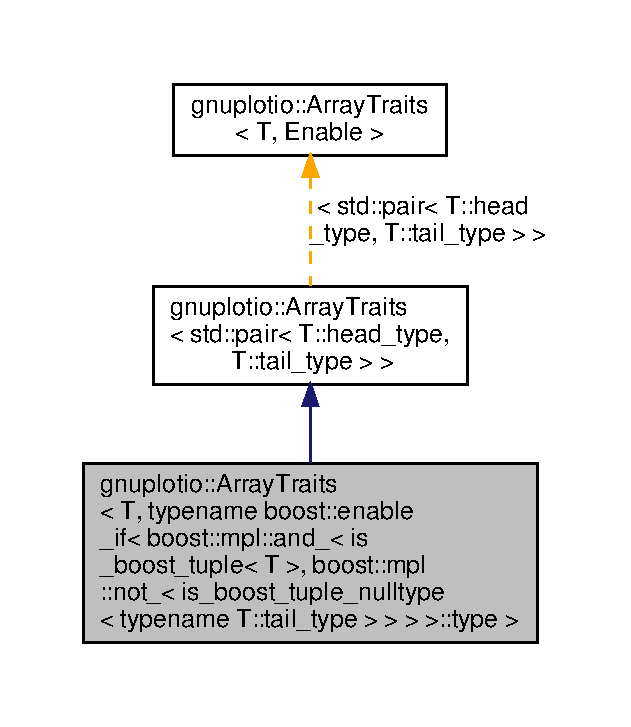
\includegraphics[width=303pt]{classgnuplotio_1_1_array_traits_3_01_t_00_01typename_01boost_1_1enable__if_3_01boost_1_1mpl_1_1a1581fe615c30084043274cbfdd41a619}
\end{center}
\end{figure}


Collaboration diagram for gnuplotio\+:\+:Array\+Traits$<$ T, typename boost\+:\+:enable\+\_\+if$<$ boost\+:\+:mpl\+:\+:and\+\_\+$<$ is\+\_\+boost\+\_\+tuple$<$ T $>$, boost\+:\+:mpl\+:\+:not\+\_\+$<$ is\+\_\+boost\+\_\+tuple\+\_\+nulltype$<$ typename T\+:\+:tail\+\_\+type $>$ $>$ $>$ $>$\+:\+:type $>$\+:
\nopagebreak
\begin{figure}[H]
\begin{center}
\leavevmode
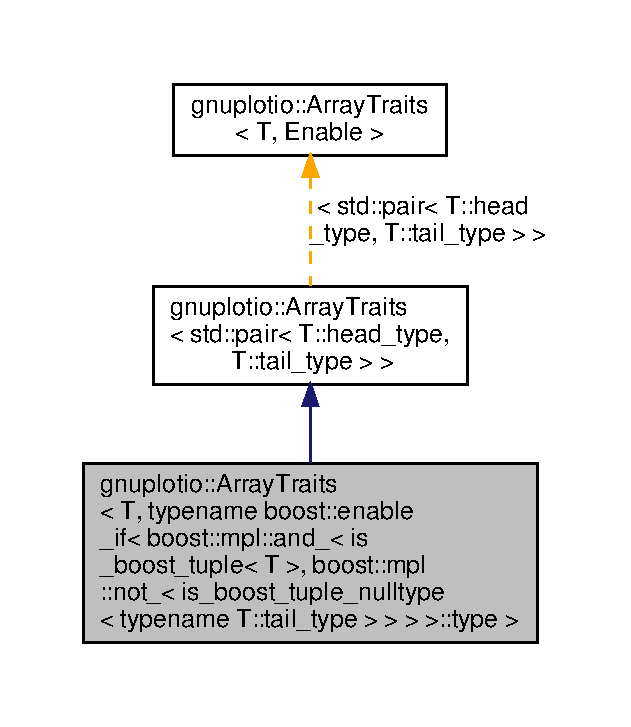
\includegraphics[width=303pt]{classgnuplotio_1_1_array_traits_3_01_t_00_01typename_01boost_1_1enable__if_3_01boost_1_1mpl_1_1aba4443da019311cdd4c31f059136bc6c}
\end{center}
\end{figure}
\subsection*{Public Types}
\begin{DoxyCompactItemize}
\item 
typedef T\+::head\+\_\+type \hyperlink{classgnuplotio_1_1_array_traits_3_01_t_00_01typename_01boost_1_1enable__if_3_01boost_1_1mpl_1_1a8de3a8fe198d85f7f5d28b9a2f5bf229_ab56761f05b74be318cc7becbc59348df}{HT}
\item 
typedef T\+::tail\+\_\+type \hyperlink{classgnuplotio_1_1_array_traits_3_01_t_00_01typename_01boost_1_1enable__if_3_01boost_1_1mpl_1_1a8de3a8fe198d85f7f5d28b9a2f5bf229_a16316f598ab57b0b7ceea99dcd34632e}{TT}
\item 
typedef \hyperlink{classgnuplotio_1_1_array_traits}{Array\+Traits}$<$ typename std\+::pair$<$ \hyperlink{classgnuplotio_1_1_array_traits_3_01_t_00_01typename_01boost_1_1enable__if_3_01boost_1_1mpl_1_1a8de3a8fe198d85f7f5d28b9a2f5bf229_ab56761f05b74be318cc7becbc59348df}{HT}, \hyperlink{classgnuplotio_1_1_array_traits_3_01_t_00_01typename_01boost_1_1enable__if_3_01boost_1_1mpl_1_1a8de3a8fe198d85f7f5d28b9a2f5bf229_a16316f598ab57b0b7ceea99dcd34632e}{TT} $>$ $>$ \hyperlink{classgnuplotio_1_1_array_traits_3_01_t_00_01typename_01boost_1_1enable__if_3_01boost_1_1mpl_1_1a8de3a8fe198d85f7f5d28b9a2f5bf229_aad44f59a1d618b863442a9fdaa83d142}{parent}
\end{DoxyCompactItemize}
\subsection*{Static Public Member Functions}
\begin{DoxyCompactItemize}
\item 
static \hyperlink{classgnuplotio_1_1_array_traits_ae53464a5175c03deec403392b8dcb3c5}{parent\+::range\+\_\+type} \hyperlink{classgnuplotio_1_1_array_traits_3_01_t_00_01typename_01boost_1_1enable__if_3_01boost_1_1mpl_1_1a8de3a8fe198d85f7f5d28b9a2f5bf229_aec07e01edbb46f5f283d5b6af068c0f2}{get\+\_\+range} (const T \&arg)
\end{DoxyCompactItemize}
\subsection*{Additional Inherited Members}


\subsection{Detailed Description}
\subsubsection*{template$<$typename T$>$\newline
class gnuplotio\+::\+Array\+Traits$<$ T, typename boost\+::enable\+\_\+if$<$ boost\+::mpl\+::and\+\_\+$<$ is\+\_\+boost\+\_\+tuple$<$ T $>$, boost\+::mpl\+::not\+\_\+$<$ is\+\_\+boost\+\_\+tuple\+\_\+nulltype$<$ typename T\+::tail\+\_\+type $>$ $>$ $>$ $>$\+::type $>$}



Definition at line 994 of file gnuplot-\/iostream.\+h.



\subsection{Member Typedef Documentation}
\mbox{\Hypertarget{classgnuplotio_1_1_array_traits_3_01_t_00_01typename_01boost_1_1enable__if_3_01boost_1_1mpl_1_1a8de3a8fe198d85f7f5d28b9a2f5bf229_ab56761f05b74be318cc7becbc59348df}\label{classgnuplotio_1_1_array_traits_3_01_t_00_01typename_01boost_1_1enable__if_3_01boost_1_1mpl_1_1a8de3a8fe198d85f7f5d28b9a2f5bf229_ab56761f05b74be318cc7becbc59348df}} 
\index{gnuplotio\+::\+Array\+Traits$<$ T, typename boost\+::enable\+\_\+if$<$ boost\+::mpl\+::and\+\_\+$<$ is\+\_\+boost\+\_\+tuple$<$ T $>$, boost\+::mpl\+::not\+\_\+$<$ is\+\_\+boost\+\_\+tuple\+\_\+nulltype$<$ typename T\+::tail\+\_\+type $>$ $>$ $>$ $>$\+::type $>$@{gnuplotio\+::\+Array\+Traits$<$ T, typename boost\+::enable\+\_\+if$<$ boost\+::mpl\+::and\+\_\+$<$ is\+\_\+boost\+\_\+tuple$<$ T $>$, boost\+::mpl\+::not\+\_\+$<$ is\+\_\+boost\+\_\+tuple\+\_\+nulltype$<$ typename T\+::tail\+\_\+type $>$ $>$ $>$ $>$\+::type $>$}!HT@{HT}}
\index{HT@{HT}!gnuplotio\+::\+Array\+Traits$<$ T, typename boost\+::enable\+\_\+if$<$ boost\+::mpl\+::and\+\_\+$<$ is\+\_\+boost\+\_\+tuple$<$ T $>$, boost\+::mpl\+::not\+\_\+$<$ is\+\_\+boost\+\_\+tuple\+\_\+nulltype$<$ typename T\+::tail\+\_\+type $>$ $>$ $>$ $>$\+::type $>$@{gnuplotio\+::\+Array\+Traits$<$ T, typename boost\+::enable\+\_\+if$<$ boost\+::mpl\+::and\+\_\+$<$ is\+\_\+boost\+\_\+tuple$<$ T $>$, boost\+::mpl\+::not\+\_\+$<$ is\+\_\+boost\+\_\+tuple\+\_\+nulltype$<$ typename T\+::tail\+\_\+type $>$ $>$ $>$ $>$\+::type $>$}}
\subsubsection{\texorpdfstring{HT}{HT}}
{\footnotesize\ttfamily template$<$typename T $>$ \\
typedef T\+::head\+\_\+type \hyperlink{classgnuplotio_1_1_array_traits}{gnuplotio\+::\+Array\+Traits}$<$ T, typename boost\+::enable\+\_\+if$<$ boost\+::mpl\+::and\+\_\+$<$ \hyperlink{structgnuplotio_1_1is__boost__tuple}{is\+\_\+boost\+\_\+tuple}$<$ T $>$, boost\+::mpl\+::not\+\_\+$<$ \hyperlink{structgnuplotio_1_1is__boost__tuple__nulltype}{is\+\_\+boost\+\_\+tuple\+\_\+nulltype}$<$ typename T\+::tail\+\_\+type $>$ $>$ $>$ $>$\+::type $>$\+::\hyperlink{classgnuplotio_1_1_array_traits_3_01_t_00_01typename_01boost_1_1enable__if_3_01boost_1_1mpl_1_1a8de3a8fe198d85f7f5d28b9a2f5bf229_ab56761f05b74be318cc7becbc59348df}{HT}}



Definition at line 1008 of file gnuplot-\/iostream.\+h.

\mbox{\Hypertarget{classgnuplotio_1_1_array_traits_3_01_t_00_01typename_01boost_1_1enable__if_3_01boost_1_1mpl_1_1a8de3a8fe198d85f7f5d28b9a2f5bf229_aad44f59a1d618b863442a9fdaa83d142}\label{classgnuplotio_1_1_array_traits_3_01_t_00_01typename_01boost_1_1enable__if_3_01boost_1_1mpl_1_1a8de3a8fe198d85f7f5d28b9a2f5bf229_aad44f59a1d618b863442a9fdaa83d142}} 
\index{gnuplotio\+::\+Array\+Traits$<$ T, typename boost\+::enable\+\_\+if$<$ boost\+::mpl\+::and\+\_\+$<$ is\+\_\+boost\+\_\+tuple$<$ T $>$, boost\+::mpl\+::not\+\_\+$<$ is\+\_\+boost\+\_\+tuple\+\_\+nulltype$<$ typename T\+::tail\+\_\+type $>$ $>$ $>$ $>$\+::type $>$@{gnuplotio\+::\+Array\+Traits$<$ T, typename boost\+::enable\+\_\+if$<$ boost\+::mpl\+::and\+\_\+$<$ is\+\_\+boost\+\_\+tuple$<$ T $>$, boost\+::mpl\+::not\+\_\+$<$ is\+\_\+boost\+\_\+tuple\+\_\+nulltype$<$ typename T\+::tail\+\_\+type $>$ $>$ $>$ $>$\+::type $>$}!parent@{parent}}
\index{parent@{parent}!gnuplotio\+::\+Array\+Traits$<$ T, typename boost\+::enable\+\_\+if$<$ boost\+::mpl\+::and\+\_\+$<$ is\+\_\+boost\+\_\+tuple$<$ T $>$, boost\+::mpl\+::not\+\_\+$<$ is\+\_\+boost\+\_\+tuple\+\_\+nulltype$<$ typename T\+::tail\+\_\+type $>$ $>$ $>$ $>$\+::type $>$@{gnuplotio\+::\+Array\+Traits$<$ T, typename boost\+::enable\+\_\+if$<$ boost\+::mpl\+::and\+\_\+$<$ is\+\_\+boost\+\_\+tuple$<$ T $>$, boost\+::mpl\+::not\+\_\+$<$ is\+\_\+boost\+\_\+tuple\+\_\+nulltype$<$ typename T\+::tail\+\_\+type $>$ $>$ $>$ $>$\+::type $>$}}
\subsubsection{\texorpdfstring{parent}{parent}}
{\footnotesize\ttfamily template$<$typename T $>$ \\
typedef \hyperlink{classgnuplotio_1_1_array_traits}{Array\+Traits}$<$typename std\+::pair$<$\hyperlink{classgnuplotio_1_1_array_traits_3_01_t_00_01typename_01boost_1_1enable__if_3_01boost_1_1mpl_1_1a8de3a8fe198d85f7f5d28b9a2f5bf229_ab56761f05b74be318cc7becbc59348df}{HT}, \hyperlink{classgnuplotio_1_1_array_traits_3_01_t_00_01typename_01boost_1_1enable__if_3_01boost_1_1mpl_1_1a8de3a8fe198d85f7f5d28b9a2f5bf229_a16316f598ab57b0b7ceea99dcd34632e}{TT}$>$ $>$ \hyperlink{classgnuplotio_1_1_array_traits}{gnuplotio\+::\+Array\+Traits}$<$ T, typename boost\+::enable\+\_\+if$<$ boost\+::mpl\+::and\+\_\+$<$ \hyperlink{structgnuplotio_1_1is__boost__tuple}{is\+\_\+boost\+\_\+tuple}$<$ T $>$, boost\+::mpl\+::not\+\_\+$<$ \hyperlink{structgnuplotio_1_1is__boost__tuple__nulltype}{is\+\_\+boost\+\_\+tuple\+\_\+nulltype}$<$ typename T\+::tail\+\_\+type $>$ $>$ $>$ $>$\+::type $>$\+::\hyperlink{classgnuplotio_1_1_array_traits_3_01_t_00_01typename_01boost_1_1enable__if_3_01boost_1_1mpl_1_1a8de3a8fe198d85f7f5d28b9a2f5bf229_aad44f59a1d618b863442a9fdaa83d142}{parent}}



Definition at line 1011 of file gnuplot-\/iostream.\+h.

\mbox{\Hypertarget{classgnuplotio_1_1_array_traits_3_01_t_00_01typename_01boost_1_1enable__if_3_01boost_1_1mpl_1_1a8de3a8fe198d85f7f5d28b9a2f5bf229_a16316f598ab57b0b7ceea99dcd34632e}\label{classgnuplotio_1_1_array_traits_3_01_t_00_01typename_01boost_1_1enable__if_3_01boost_1_1mpl_1_1a8de3a8fe198d85f7f5d28b9a2f5bf229_a16316f598ab57b0b7ceea99dcd34632e}} 
\index{gnuplotio\+::\+Array\+Traits$<$ T, typename boost\+::enable\+\_\+if$<$ boost\+::mpl\+::and\+\_\+$<$ is\+\_\+boost\+\_\+tuple$<$ T $>$, boost\+::mpl\+::not\+\_\+$<$ is\+\_\+boost\+\_\+tuple\+\_\+nulltype$<$ typename T\+::tail\+\_\+type $>$ $>$ $>$ $>$\+::type $>$@{gnuplotio\+::\+Array\+Traits$<$ T, typename boost\+::enable\+\_\+if$<$ boost\+::mpl\+::and\+\_\+$<$ is\+\_\+boost\+\_\+tuple$<$ T $>$, boost\+::mpl\+::not\+\_\+$<$ is\+\_\+boost\+\_\+tuple\+\_\+nulltype$<$ typename T\+::tail\+\_\+type $>$ $>$ $>$ $>$\+::type $>$}!TT@{TT}}
\index{TT@{TT}!gnuplotio\+::\+Array\+Traits$<$ T, typename boost\+::enable\+\_\+if$<$ boost\+::mpl\+::and\+\_\+$<$ is\+\_\+boost\+\_\+tuple$<$ T $>$, boost\+::mpl\+::not\+\_\+$<$ is\+\_\+boost\+\_\+tuple\+\_\+nulltype$<$ typename T\+::tail\+\_\+type $>$ $>$ $>$ $>$\+::type $>$@{gnuplotio\+::\+Array\+Traits$<$ T, typename boost\+::enable\+\_\+if$<$ boost\+::mpl\+::and\+\_\+$<$ is\+\_\+boost\+\_\+tuple$<$ T $>$, boost\+::mpl\+::not\+\_\+$<$ is\+\_\+boost\+\_\+tuple\+\_\+nulltype$<$ typename T\+::tail\+\_\+type $>$ $>$ $>$ $>$\+::type $>$}}
\subsubsection{\texorpdfstring{TT}{TT}}
{\footnotesize\ttfamily template$<$typename T $>$ \\
typedef T\+::tail\+\_\+type \hyperlink{classgnuplotio_1_1_array_traits}{gnuplotio\+::\+Array\+Traits}$<$ T, typename boost\+::enable\+\_\+if$<$ boost\+::mpl\+::and\+\_\+$<$ \hyperlink{structgnuplotio_1_1is__boost__tuple}{is\+\_\+boost\+\_\+tuple}$<$ T $>$, boost\+::mpl\+::not\+\_\+$<$ \hyperlink{structgnuplotio_1_1is__boost__tuple__nulltype}{is\+\_\+boost\+\_\+tuple\+\_\+nulltype}$<$ typename T\+::tail\+\_\+type $>$ $>$ $>$ $>$\+::type $>$\+::\hyperlink{classgnuplotio_1_1_array_traits_3_01_t_00_01typename_01boost_1_1enable__if_3_01boost_1_1mpl_1_1a8de3a8fe198d85f7f5d28b9a2f5bf229_a16316f598ab57b0b7ceea99dcd34632e}{TT}}



Definition at line 1009 of file gnuplot-\/iostream.\+h.



\subsection{Member Function Documentation}
\mbox{\Hypertarget{classgnuplotio_1_1_array_traits_3_01_t_00_01typename_01boost_1_1enable__if_3_01boost_1_1mpl_1_1a8de3a8fe198d85f7f5d28b9a2f5bf229_aec07e01edbb46f5f283d5b6af068c0f2}\label{classgnuplotio_1_1_array_traits_3_01_t_00_01typename_01boost_1_1enable__if_3_01boost_1_1mpl_1_1a8de3a8fe198d85f7f5d28b9a2f5bf229_aec07e01edbb46f5f283d5b6af068c0f2}} 
\index{gnuplotio\+::\+Array\+Traits$<$ T, typename boost\+::enable\+\_\+if$<$ boost\+::mpl\+::and\+\_\+$<$ is\+\_\+boost\+\_\+tuple$<$ T $>$, boost\+::mpl\+::not\+\_\+$<$ is\+\_\+boost\+\_\+tuple\+\_\+nulltype$<$ typename T\+::tail\+\_\+type $>$ $>$ $>$ $>$\+::type $>$@{gnuplotio\+::\+Array\+Traits$<$ T, typename boost\+::enable\+\_\+if$<$ boost\+::mpl\+::and\+\_\+$<$ is\+\_\+boost\+\_\+tuple$<$ T $>$, boost\+::mpl\+::not\+\_\+$<$ is\+\_\+boost\+\_\+tuple\+\_\+nulltype$<$ typename T\+::tail\+\_\+type $>$ $>$ $>$ $>$\+::type $>$}!get\+\_\+range@{get\+\_\+range}}
\index{get\+\_\+range@{get\+\_\+range}!gnuplotio\+::\+Array\+Traits$<$ T, typename boost\+::enable\+\_\+if$<$ boost\+::mpl\+::and\+\_\+$<$ is\+\_\+boost\+\_\+tuple$<$ T $>$, boost\+::mpl\+::not\+\_\+$<$ is\+\_\+boost\+\_\+tuple\+\_\+nulltype$<$ typename T\+::tail\+\_\+type $>$ $>$ $>$ $>$\+::type $>$@{gnuplotio\+::\+Array\+Traits$<$ T, typename boost\+::enable\+\_\+if$<$ boost\+::mpl\+::and\+\_\+$<$ is\+\_\+boost\+\_\+tuple$<$ T $>$, boost\+::mpl\+::not\+\_\+$<$ is\+\_\+boost\+\_\+tuple\+\_\+nulltype$<$ typename T\+::tail\+\_\+type $>$ $>$ $>$ $>$\+::type $>$}}
\subsubsection{\texorpdfstring{get\+\_\+range()}{get\_range()}}
{\footnotesize\ttfamily template$<$typename T $>$ \\
static \hyperlink{classgnuplotio_1_1_array_traits_ae53464a5175c03deec403392b8dcb3c5}{parent\+::range\+\_\+type} \hyperlink{classgnuplotio_1_1_array_traits}{gnuplotio\+::\+Array\+Traits}$<$ T, typename boost\+::enable\+\_\+if$<$ boost\+::mpl\+::and\+\_\+$<$ \hyperlink{structgnuplotio_1_1is__boost__tuple}{is\+\_\+boost\+\_\+tuple}$<$ T $>$, boost\+::mpl\+::not\+\_\+$<$ \hyperlink{structgnuplotio_1_1is__boost__tuple__nulltype}{is\+\_\+boost\+\_\+tuple\+\_\+nulltype}$<$ typename T\+::tail\+\_\+type $>$ $>$ $>$ $>$\+::type $>$\+::get\+\_\+range (\begin{DoxyParamCaption}\item[{const T \&}]{arg }\end{DoxyParamCaption})\hspace{0.3cm}{\ttfamily [inline]}, {\ttfamily [static]}}



Definition at line 1013 of file gnuplot-\/iostream.\+h.



The documentation for this class was generated from the following file\+:\begin{DoxyCompactItemize}
\item 
include/\hyperlink{gnuplot-iostream_8h}{gnuplot-\/iostream.\+h}\end{DoxyCompactItemize}

\hypertarget{classgnuplotio_1_1_array_traits_3_01_t_00_01typename_01boost_1_1enable__if_3_01boost_1_1mpl_1_1ad3fa8e75dccbaae12a06d17831678a88}{}\section{gnuplotio\+:\+:Array\+Traits$<$ T, typename boost\+:\+:enable\+\_\+if$<$ boost\+:\+:mpl\+:\+:and\+\_\+$<$ is\+\_\+boost\+\_\+tuple$<$ T $>$, is\+\_\+boost\+\_\+tuple\+\_\+nulltype$<$ typename T\+:\+:tail\+\_\+type $>$ $>$ $>$\+:\+:type $>$ Class Template Reference}
\label{classgnuplotio_1_1_array_traits_3_01_t_00_01typename_01boost_1_1enable__if_3_01boost_1_1mpl_1_1ad3fa8e75dccbaae12a06d17831678a88}\index{gnuplotio\+::\+Array\+Traits$<$ T, typename boost\+::enable\+\_\+if$<$ boost\+::mpl\+::and\+\_\+$<$ is\+\_\+boost\+\_\+tuple$<$ T $>$, is\+\_\+boost\+\_\+tuple\+\_\+nulltype$<$ typename T\+::tail\+\_\+type $>$ $>$ $>$\+::type $>$@{gnuplotio\+::\+Array\+Traits$<$ T, typename boost\+::enable\+\_\+if$<$ boost\+::mpl\+::and\+\_\+$<$ is\+\_\+boost\+\_\+tuple$<$ T $>$, is\+\_\+boost\+\_\+tuple\+\_\+nulltype$<$ typename T\+::tail\+\_\+type $>$ $>$ $>$\+::type $>$}}


{\ttfamily \#include $<$gnuplot-\/iostream.\+h$>$}



Inheritance diagram for gnuplotio\+:\+:Array\+Traits$<$ T, typename boost\+:\+:enable\+\_\+if$<$ boost\+:\+:mpl\+:\+:and\+\_\+$<$ is\+\_\+boost\+\_\+tuple$<$ T $>$, is\+\_\+boost\+\_\+tuple\+\_\+nulltype$<$ typename T\+:\+:tail\+\_\+type $>$ $>$ $>$\+:\+:type $>$\+:
\nopagebreak
\begin{figure}[H]
\begin{center}
\leavevmode
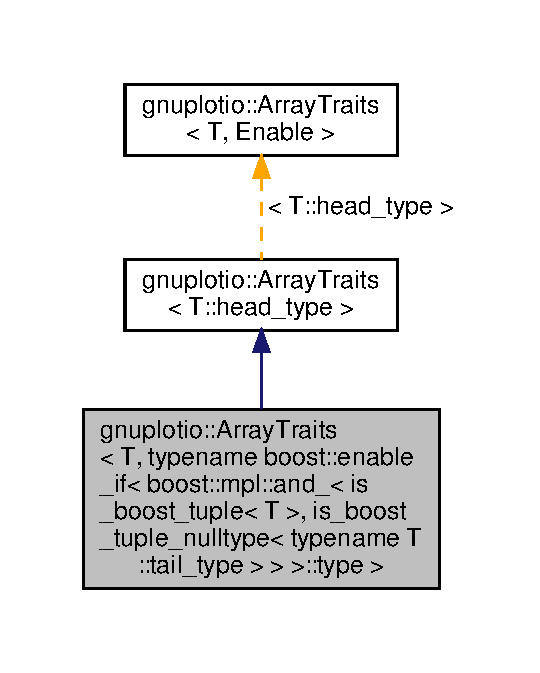
\includegraphics[width=259pt]{classgnuplotio_1_1_array_traits_3_01_t_00_01typename_01boost_1_1enable__if_3_01boost_1_1mpl_1_1aea65f5b28bab149b37099425ffdc1482}
\end{center}
\end{figure}


Collaboration diagram for gnuplotio\+:\+:Array\+Traits$<$ T, typename boost\+:\+:enable\+\_\+if$<$ boost\+:\+:mpl\+:\+:and\+\_\+$<$ is\+\_\+boost\+\_\+tuple$<$ T $>$, is\+\_\+boost\+\_\+tuple\+\_\+nulltype$<$ typename T\+:\+:tail\+\_\+type $>$ $>$ $>$\+:\+:type $>$\+:
\nopagebreak
\begin{figure}[H]
\begin{center}
\leavevmode
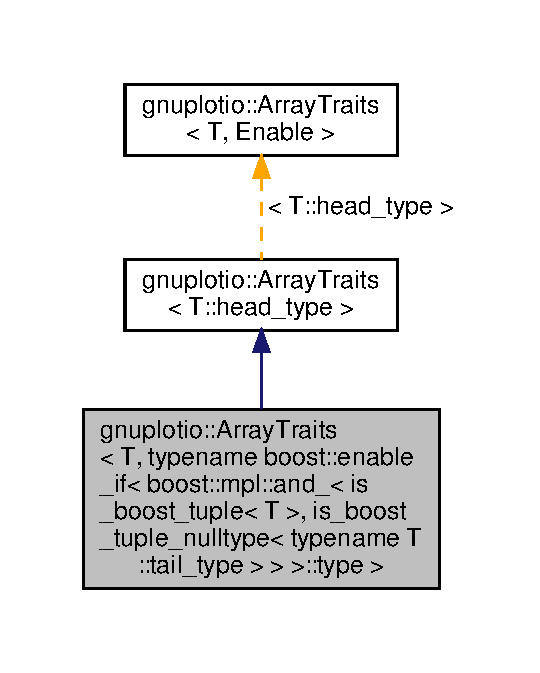
\includegraphics[width=259pt]{classgnuplotio_1_1_array_traits_3_01_t_00_01typename_01boost_1_1enable__if_3_01boost_1_1mpl_1_1a7c2880846d33bb3586d5921312165f33}
\end{center}
\end{figure}
\subsection*{Static Public Member Functions}
\begin{DoxyCompactItemize}
\item 
static \hyperlink{classgnuplotio_1_1_array_traits_ae53464a5175c03deec403392b8dcb3c5}{parent\+::range\+\_\+type} \hyperlink{classgnuplotio_1_1_array_traits_3_01_t_00_01typename_01boost_1_1enable__if_3_01boost_1_1mpl_1_1ad3fa8e75dccbaae12a06d17831678a88_ad0485dd16a9d54a4eb75bf3e75b1facd}{get\+\_\+range} (const T \&arg)
\end{DoxyCompactItemize}
\subsection*{Private Types}
\begin{DoxyCompactItemize}
\item 
typedef T\+::head\+\_\+type \hyperlink{classgnuplotio_1_1_array_traits_3_01_t_00_01typename_01boost_1_1enable__if_3_01boost_1_1mpl_1_1ad3fa8e75dccbaae12a06d17831678a88_a46da790e18efa0f6eb7716ea36261c13}{HT}
\item 
typedef \hyperlink{classgnuplotio_1_1_array_traits}{Array\+Traits}$<$ \hyperlink{classgnuplotio_1_1_array_traits_3_01_t_00_01typename_01boost_1_1enable__if_3_01boost_1_1mpl_1_1ad3fa8e75dccbaae12a06d17831678a88_a46da790e18efa0f6eb7716ea36261c13}{HT} $>$ \hyperlink{classgnuplotio_1_1_array_traits_3_01_t_00_01typename_01boost_1_1enable__if_3_01boost_1_1mpl_1_1ad3fa8e75dccbaae12a06d17831678a88_a55f28a139e49666b667bc6727c14e985}{parent}
\end{DoxyCompactItemize}
\subsection*{Additional Inherited Members}


\subsection{Detailed Description}
\subsubsection*{template$<$typename T$>$\newline
class gnuplotio\+::\+Array\+Traits$<$ T, typename boost\+::enable\+\_\+if$<$ boost\+::mpl\+::and\+\_\+$<$ is\+\_\+boost\+\_\+tuple$<$ T $>$, is\+\_\+boost\+\_\+tuple\+\_\+nulltype$<$ typename T\+::tail\+\_\+type $>$ $>$ $>$\+::type $>$}



Definition at line 1022 of file gnuplot-\/iostream.\+h.



\subsection{Member Typedef Documentation}
\mbox{\Hypertarget{classgnuplotio_1_1_array_traits_3_01_t_00_01typename_01boost_1_1enable__if_3_01boost_1_1mpl_1_1ad3fa8e75dccbaae12a06d17831678a88_a46da790e18efa0f6eb7716ea36261c13}\label{classgnuplotio_1_1_array_traits_3_01_t_00_01typename_01boost_1_1enable__if_3_01boost_1_1mpl_1_1ad3fa8e75dccbaae12a06d17831678a88_a46da790e18efa0f6eb7716ea36261c13}} 
\index{gnuplotio\+::\+Array\+Traits$<$ T, typename boost\+::enable\+\_\+if$<$ boost\+::mpl\+::and\+\_\+$<$ is\+\_\+boost\+\_\+tuple$<$ T $>$, is\+\_\+boost\+\_\+tuple\+\_\+nulltype$<$ typename T\+::tail\+\_\+type $>$ $>$ $>$\+::type $>$@{gnuplotio\+::\+Array\+Traits$<$ T, typename boost\+::enable\+\_\+if$<$ boost\+::mpl\+::and\+\_\+$<$ is\+\_\+boost\+\_\+tuple$<$ T $>$, is\+\_\+boost\+\_\+tuple\+\_\+nulltype$<$ typename T\+::tail\+\_\+type $>$ $>$ $>$\+::type $>$}!HT@{HT}}
\index{HT@{HT}!gnuplotio\+::\+Array\+Traits$<$ T, typename boost\+::enable\+\_\+if$<$ boost\+::mpl\+::and\+\_\+$<$ is\+\_\+boost\+\_\+tuple$<$ T $>$, is\+\_\+boost\+\_\+tuple\+\_\+nulltype$<$ typename T\+::tail\+\_\+type $>$ $>$ $>$\+::type $>$@{gnuplotio\+::\+Array\+Traits$<$ T, typename boost\+::enable\+\_\+if$<$ boost\+::mpl\+::and\+\_\+$<$ is\+\_\+boost\+\_\+tuple$<$ T $>$, is\+\_\+boost\+\_\+tuple\+\_\+nulltype$<$ typename T\+::tail\+\_\+type $>$ $>$ $>$\+::type $>$}}
\subsubsection{\texorpdfstring{HT}{HT}}
{\footnotesize\ttfamily template$<$typename T $>$ \\
typedef T\+::head\+\_\+type \hyperlink{classgnuplotio_1_1_array_traits}{gnuplotio\+::\+Array\+Traits}$<$ T, typename boost\+::enable\+\_\+if$<$ boost\+::mpl\+::and\+\_\+$<$ \hyperlink{structgnuplotio_1_1is__boost__tuple}{is\+\_\+boost\+\_\+tuple}$<$ T $>$, \hyperlink{structgnuplotio_1_1is__boost__tuple__nulltype}{is\+\_\+boost\+\_\+tuple\+\_\+nulltype}$<$ typename T\+::tail\+\_\+type $>$ $>$ $>$\+::type $>$\+::\hyperlink{classgnuplotio_1_1_array_traits_3_01_t_00_01typename_01boost_1_1enable__if_3_01boost_1_1mpl_1_1ad3fa8e75dccbaae12a06d17831678a88_a46da790e18efa0f6eb7716ea36261c13}{HT}\hspace{0.3cm}{\ttfamily [private]}}



Definition at line 1032 of file gnuplot-\/iostream.\+h.

\mbox{\Hypertarget{classgnuplotio_1_1_array_traits_3_01_t_00_01typename_01boost_1_1enable__if_3_01boost_1_1mpl_1_1ad3fa8e75dccbaae12a06d17831678a88_a55f28a139e49666b667bc6727c14e985}\label{classgnuplotio_1_1_array_traits_3_01_t_00_01typename_01boost_1_1enable__if_3_01boost_1_1mpl_1_1ad3fa8e75dccbaae12a06d17831678a88_a55f28a139e49666b667bc6727c14e985}} 
\index{gnuplotio\+::\+Array\+Traits$<$ T, typename boost\+::enable\+\_\+if$<$ boost\+::mpl\+::and\+\_\+$<$ is\+\_\+boost\+\_\+tuple$<$ T $>$, is\+\_\+boost\+\_\+tuple\+\_\+nulltype$<$ typename T\+::tail\+\_\+type $>$ $>$ $>$\+::type $>$@{gnuplotio\+::\+Array\+Traits$<$ T, typename boost\+::enable\+\_\+if$<$ boost\+::mpl\+::and\+\_\+$<$ is\+\_\+boost\+\_\+tuple$<$ T $>$, is\+\_\+boost\+\_\+tuple\+\_\+nulltype$<$ typename T\+::tail\+\_\+type $>$ $>$ $>$\+::type $>$}!parent@{parent}}
\index{parent@{parent}!gnuplotio\+::\+Array\+Traits$<$ T, typename boost\+::enable\+\_\+if$<$ boost\+::mpl\+::and\+\_\+$<$ is\+\_\+boost\+\_\+tuple$<$ T $>$, is\+\_\+boost\+\_\+tuple\+\_\+nulltype$<$ typename T\+::tail\+\_\+type $>$ $>$ $>$\+::type $>$@{gnuplotio\+::\+Array\+Traits$<$ T, typename boost\+::enable\+\_\+if$<$ boost\+::mpl\+::and\+\_\+$<$ is\+\_\+boost\+\_\+tuple$<$ T $>$, is\+\_\+boost\+\_\+tuple\+\_\+nulltype$<$ typename T\+::tail\+\_\+type $>$ $>$ $>$\+::type $>$}}
\subsubsection{\texorpdfstring{parent}{parent}}
{\footnotesize\ttfamily template$<$typename T $>$ \\
typedef \hyperlink{classgnuplotio_1_1_array_traits}{Array\+Traits}$<$\hyperlink{classgnuplotio_1_1_array_traits_3_01_t_00_01typename_01boost_1_1enable__if_3_01boost_1_1mpl_1_1ad3fa8e75dccbaae12a06d17831678a88_a46da790e18efa0f6eb7716ea36261c13}{HT}$>$ \hyperlink{classgnuplotio_1_1_array_traits}{gnuplotio\+::\+Array\+Traits}$<$ T, typename boost\+::enable\+\_\+if$<$ boost\+::mpl\+::and\+\_\+$<$ \hyperlink{structgnuplotio_1_1is__boost__tuple}{is\+\_\+boost\+\_\+tuple}$<$ T $>$, \hyperlink{structgnuplotio_1_1is__boost__tuple__nulltype}{is\+\_\+boost\+\_\+tuple\+\_\+nulltype}$<$ typename T\+::tail\+\_\+type $>$ $>$ $>$\+::type $>$\+::\hyperlink{classgnuplotio_1_1_array_traits_3_01_t_00_01typename_01boost_1_1enable__if_3_01boost_1_1mpl_1_1ad3fa8e75dccbaae12a06d17831678a88_a55f28a139e49666b667bc6727c14e985}{parent}\hspace{0.3cm}{\ttfamily [private]}}



Definition at line 1034 of file gnuplot-\/iostream.\+h.



\subsection{Member Function Documentation}
\mbox{\Hypertarget{classgnuplotio_1_1_array_traits_3_01_t_00_01typename_01boost_1_1enable__if_3_01boost_1_1mpl_1_1ad3fa8e75dccbaae12a06d17831678a88_ad0485dd16a9d54a4eb75bf3e75b1facd}\label{classgnuplotio_1_1_array_traits_3_01_t_00_01typename_01boost_1_1enable__if_3_01boost_1_1mpl_1_1ad3fa8e75dccbaae12a06d17831678a88_ad0485dd16a9d54a4eb75bf3e75b1facd}} 
\index{gnuplotio\+::\+Array\+Traits$<$ T, typename boost\+::enable\+\_\+if$<$ boost\+::mpl\+::and\+\_\+$<$ is\+\_\+boost\+\_\+tuple$<$ T $>$, is\+\_\+boost\+\_\+tuple\+\_\+nulltype$<$ typename T\+::tail\+\_\+type $>$ $>$ $>$\+::type $>$@{gnuplotio\+::\+Array\+Traits$<$ T, typename boost\+::enable\+\_\+if$<$ boost\+::mpl\+::and\+\_\+$<$ is\+\_\+boost\+\_\+tuple$<$ T $>$, is\+\_\+boost\+\_\+tuple\+\_\+nulltype$<$ typename T\+::tail\+\_\+type $>$ $>$ $>$\+::type $>$}!get\+\_\+range@{get\+\_\+range}}
\index{get\+\_\+range@{get\+\_\+range}!gnuplotio\+::\+Array\+Traits$<$ T, typename boost\+::enable\+\_\+if$<$ boost\+::mpl\+::and\+\_\+$<$ is\+\_\+boost\+\_\+tuple$<$ T $>$, is\+\_\+boost\+\_\+tuple\+\_\+nulltype$<$ typename T\+::tail\+\_\+type $>$ $>$ $>$\+::type $>$@{gnuplotio\+::\+Array\+Traits$<$ T, typename boost\+::enable\+\_\+if$<$ boost\+::mpl\+::and\+\_\+$<$ is\+\_\+boost\+\_\+tuple$<$ T $>$, is\+\_\+boost\+\_\+tuple\+\_\+nulltype$<$ typename T\+::tail\+\_\+type $>$ $>$ $>$\+::type $>$}}
\subsubsection{\texorpdfstring{get\+\_\+range()}{get\_range()}}
{\footnotesize\ttfamily template$<$typename T $>$ \\
static \hyperlink{classgnuplotio_1_1_array_traits_ae53464a5175c03deec403392b8dcb3c5}{parent\+::range\+\_\+type} \hyperlink{classgnuplotio_1_1_array_traits}{gnuplotio\+::\+Array\+Traits}$<$ T, typename boost\+::enable\+\_\+if$<$ boost\+::mpl\+::and\+\_\+$<$ \hyperlink{structgnuplotio_1_1is__boost__tuple}{is\+\_\+boost\+\_\+tuple}$<$ T $>$, \hyperlink{structgnuplotio_1_1is__boost__tuple__nulltype}{is\+\_\+boost\+\_\+tuple\+\_\+nulltype}$<$ typename T\+::tail\+\_\+type $>$ $>$ $>$\+::type $>$\+::get\+\_\+range (\begin{DoxyParamCaption}\item[{const T \&}]{arg }\end{DoxyParamCaption})\hspace{0.3cm}{\ttfamily [inline]}, {\ttfamily [static]}}



Definition at line 1037 of file gnuplot-\/iostream.\+h.



References gnuplotio\+::\+Array\+Traits$<$ T, Enable $>$\+::get\+\_\+range().

Here is the call graph for this function\+:\nopagebreak
\begin{figure}[H]
\begin{center}
\leavevmode
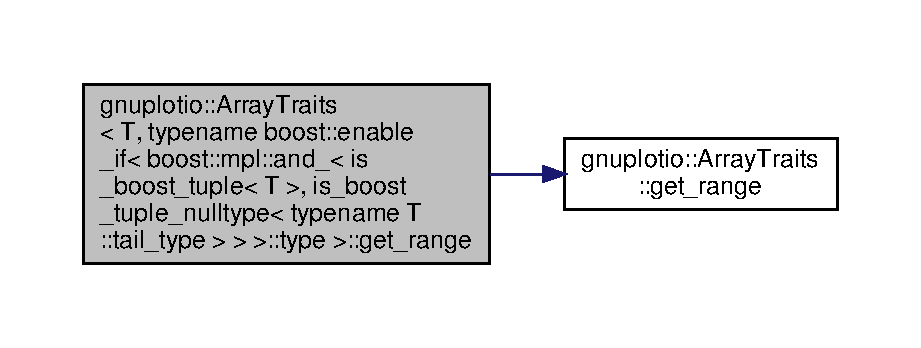
\includegraphics[width=350pt]{classgnuplotio_1_1_array_traits_3_01_t_00_01typename_01boost_1_1enable__if_3_01boost_1_1mpl_1_1ad3fa8e75dccbaae12a06d17831678a88_ad0485dd16a9d54a4eb75bf3e75b1facd_cgraph}
\end{center}
\end{figure}


The documentation for this class was generated from the following file\+:\begin{DoxyCompactItemize}
\item 
include/\hyperlink{gnuplot-iostream_8h}{gnuplot-\/iostream.\+h}\end{DoxyCompactItemize}

\hypertarget{classgnuplotio_1_1_array_traits_3_01_t_00_01typename_01boost_1_1enable__if_3_01is__like__stl__co9e1736bbd08cd58c6993ab613a998887}{}\doxysection{gnuplotio\+::Array\+Traits$<$ T, typename boost\+::enable\+\_\+if$<$ is\+\_\+like\+\_\+stl\+\_\+container$<$ T $>$ $>$\+::type $>$ Class Template Reference}
\label{classgnuplotio_1_1_array_traits_3_01_t_00_01typename_01boost_1_1enable__if_3_01is__like__stl__co9e1736bbd08cd58c6993ab613a998887}\index{gnuplotio::ArrayTraits$<$ T, typename boost::enable\_if$<$ is\_like\_stl\_container$<$ T $>$ $>$::type $>$@{gnuplotio::ArrayTraits$<$ T, typename boost::enable\_if$<$ is\_like\_stl\_container$<$ T $>$ $>$::type $>$}}


{\ttfamily \#include $<$gnuplot-\/iostream.\+h$>$}



Inheritance diagram for gnuplotio\+::Array\+Traits$<$ T, typename boost\+::enable\+\_\+if$<$ is\+\_\+like\+\_\+stl\+\_\+container$<$ T $>$ $>$\+::type $>$\+:\nopagebreak
\begin{figure}[H]
\begin{center}
\leavevmode
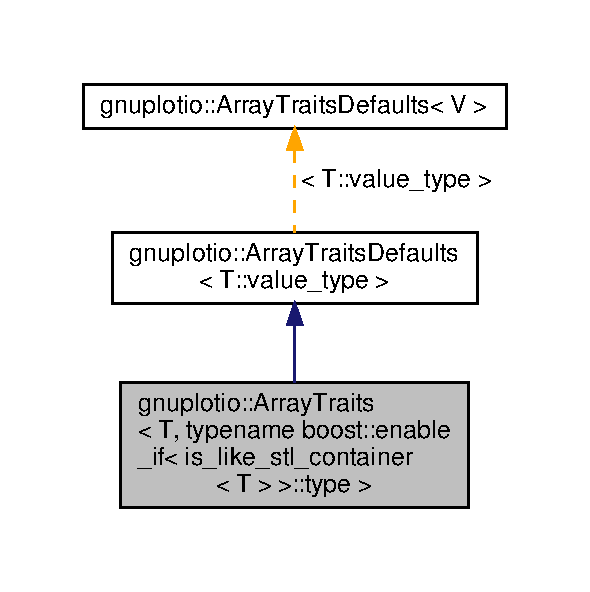
\includegraphics[width=307pt]{classgnuplotio_1_1_array_traits_3_01_t_00_01typename_01boost_1_1enable__if_3_01is__like__stl__co39a918c94e39b553da961d4c081ad747}
\end{center}
\end{figure}


Collaboration diagram for gnuplotio\+::Array\+Traits$<$ T, typename boost\+::enable\+\_\+if$<$ is\+\_\+like\+\_\+stl\+\_\+container$<$ T $>$ $>$\+::type $>$\+:\nopagebreak
\begin{figure}[H]
\begin{center}
\leavevmode
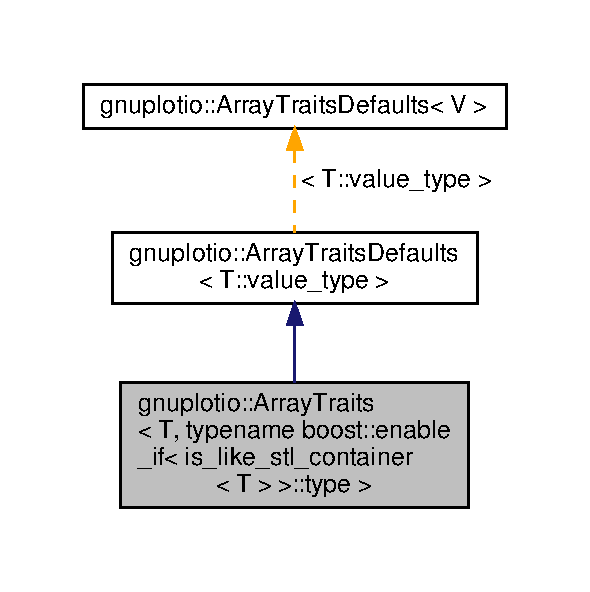
\includegraphics[width=307pt]{classgnuplotio_1_1_array_traits_3_01_t_00_01typename_01boost_1_1enable__if_3_01is__like__stl__coea0859b06c932ef4cd47658c6683d98b}
\end{center}
\end{figure}
\doxysubsection*{Public Types}
\begin{DoxyCompactItemize}
\item 
typedef \mbox{\hyperlink{classgnuplotio_1_1_iterator_range}{Iterator\+Range}}$<$ typename T\+::const\+\_\+iterator, typename \mbox{\hyperlink{classgnuplotio_1_1_array_traits_a3bcae12a7bf42af90f4946acc66f27e0}{T\+::value\+\_\+type}} $>$ \mbox{\hyperlink{classgnuplotio_1_1_array_traits_3_01_t_00_01typename_01boost_1_1enable__if_3_01is__like__stl__co9e1736bbd08cd58c6993ab613a998887_ab702072abbe018bbc90b9967ca8c4b42}{range\+\_\+type}}
\end{DoxyCompactItemize}
\doxysubsection*{Static Public Member Functions}
\begin{DoxyCompactItemize}
\item 
static \mbox{\hyperlink{classgnuplotio_1_1_array_traits_3_01_t_00_01typename_01boost_1_1enable__if_3_01is__like__stl__co9e1736bbd08cd58c6993ab613a998887_ab702072abbe018bbc90b9967ca8c4b42}{range\+\_\+type}} \mbox{\hyperlink{classgnuplotio_1_1_array_traits_3_01_t_00_01typename_01boost_1_1enable__if_3_01is__like__stl__co9e1736bbd08cd58c6993ab613a998887_a89d4150ab3c479cde972071a10acd27b}{get\+\_\+range}} (const T \&arg)
\end{DoxyCompactItemize}
\doxysubsection*{Additional Inherited Members}


\doxysubsection{Detailed Description}
\subsubsection*{template$<$typename T$>$\newline
class gnuplotio\+::\+Array\+Traits$<$ T, typename boost\+::enable\+\_\+if$<$ is\+\_\+like\+\_\+stl\+\_\+container$<$ T $>$ $>$\+::type $>$}



Definition at line 897 of file gnuplot-\/iostream.\+h.



\doxysubsection{Member Typedef Documentation}
\mbox{\Hypertarget{classgnuplotio_1_1_array_traits_3_01_t_00_01typename_01boost_1_1enable__if_3_01is__like__stl__co9e1736bbd08cd58c6993ab613a998887_ab702072abbe018bbc90b9967ca8c4b42}\label{classgnuplotio_1_1_array_traits_3_01_t_00_01typename_01boost_1_1enable__if_3_01is__like__stl__co9e1736bbd08cd58c6993ab613a998887_ab702072abbe018bbc90b9967ca8c4b42}} 
\index{gnuplotio::ArrayTraits$<$ T, typename boost::enable\_if$<$ is\_like\_stl\_container$<$ T $>$ $>$::type $>$@{gnuplotio::ArrayTraits$<$ T, typename boost::enable\_if$<$ is\_like\_stl\_container$<$ T $>$ $>$::type $>$}!range\_type@{range\_type}}
\index{range\_type@{range\_type}!gnuplotio::ArrayTraits$<$ T, typename boost::enable\_if$<$ is\_like\_stl\_container$<$ T $>$ $>$::type $>$@{gnuplotio::ArrayTraits$<$ T, typename boost::enable\_if$<$ is\_like\_stl\_container$<$ T $>$ $>$::type $>$}}
\doxysubsubsection{\texorpdfstring{range\_type}{range\_type}}
{\footnotesize\ttfamily template$<$typename T $>$ \\
typedef \mbox{\hyperlink{classgnuplotio_1_1_iterator_range}{Iterator\+Range}}$<$typename T\+::const\+\_\+iterator, typename \mbox{\hyperlink{classgnuplotio_1_1_array_traits_a3bcae12a7bf42af90f4946acc66f27e0}{T\+::value\+\_\+type}}$>$ \mbox{\hyperlink{classgnuplotio_1_1_array_traits}{gnuplotio\+::\+Array\+Traits}}$<$ T, typename boost\+::enable\+\_\+if$<$ \mbox{\hyperlink{structgnuplotio_1_1is__like__stl__container}{is\+\_\+like\+\_\+stl\+\_\+container}}$<$ T $>$ $>$\+::type $>$\+::\mbox{\hyperlink{classgnuplotio_1_1_array_traits_3_01_t_00_01typename_01boost_1_1enable__if_3_01is__like__stl__co9e1736bbd08cd58c6993ab613a998887_ab702072abbe018bbc90b9967ca8c4b42}{range\+\_\+type}}}



Definition at line 901 of file gnuplot-\/iostream.\+h.



\doxysubsection{Member Function Documentation}
\mbox{\Hypertarget{classgnuplotio_1_1_array_traits_3_01_t_00_01typename_01boost_1_1enable__if_3_01is__like__stl__co9e1736bbd08cd58c6993ab613a998887_a89d4150ab3c479cde972071a10acd27b}\label{classgnuplotio_1_1_array_traits_3_01_t_00_01typename_01boost_1_1enable__if_3_01is__like__stl__co9e1736bbd08cd58c6993ab613a998887_a89d4150ab3c479cde972071a10acd27b}} 
\index{gnuplotio::ArrayTraits$<$ T, typename boost::enable\_if$<$ is\_like\_stl\_container$<$ T $>$ $>$::type $>$@{gnuplotio::ArrayTraits$<$ T, typename boost::enable\_if$<$ is\_like\_stl\_container$<$ T $>$ $>$::type $>$}!get\_range@{get\_range}}
\index{get\_range@{get\_range}!gnuplotio::ArrayTraits$<$ T, typename boost::enable\_if$<$ is\_like\_stl\_container$<$ T $>$ $>$::type $>$@{gnuplotio::ArrayTraits$<$ T, typename boost::enable\_if$<$ is\_like\_stl\_container$<$ T $>$ $>$::type $>$}}
\doxysubsubsection{\texorpdfstring{get\_range()}{get\_range()}}
{\footnotesize\ttfamily template$<$typename T $>$ \\
static \mbox{\hyperlink{classgnuplotio_1_1_array_traits_3_01_t_00_01typename_01boost_1_1enable__if_3_01is__like__stl__co9e1736bbd08cd58c6993ab613a998887_ab702072abbe018bbc90b9967ca8c4b42}{range\+\_\+type}} \mbox{\hyperlink{classgnuplotio_1_1_array_traits}{gnuplotio\+::\+Array\+Traits}}$<$ T, typename boost\+::enable\+\_\+if$<$ \mbox{\hyperlink{structgnuplotio_1_1is__like__stl__container}{is\+\_\+like\+\_\+stl\+\_\+container}}$<$ T $>$ $>$\+::type $>$\+::get\+\_\+range (\begin{DoxyParamCaption}\item[{const T \&}]{arg }\end{DoxyParamCaption})\hspace{0.3cm}{\ttfamily [inline]}, {\ttfamily [static]}}



Definition at line 903 of file gnuplot-\/iostream.\+h.



The documentation for this class was generated from the following file\+:\begin{DoxyCompactItemize}
\item 
/home/adev/\+Documents/\+S\+T\+E\+C\+H/stewart\+\_\+platform/include/\mbox{\hyperlink{gnuplot-iostream_8h}{gnuplot-\/iostream.\+h}}\end{DoxyCompactItemize}

\hypertarget{classgnuplotio_1_1_array_traits_3_01_t[_n]_4}{}\section{gnuplotio\+:\+:Array\+Traits$<$ T\mbox{[}N\mbox{]}$>$ Class Template Reference}
\label{classgnuplotio_1_1_array_traits_3_01_t[_n]_4}\index{gnuplotio\+::\+Array\+Traits$<$ T\mbox{[}N\mbox{]}$>$@{gnuplotio\+::\+Array\+Traits$<$ T[N]$>$}}


{\ttfamily \#include $<$gnuplot-\/iostream.\+h$>$}



Inheritance diagram for gnuplotio\+:\+:Array\+Traits$<$ T\mbox{[}N\mbox{]}$>$\+:
\nopagebreak
\begin{figure}[H]
\begin{center}
\leavevmode
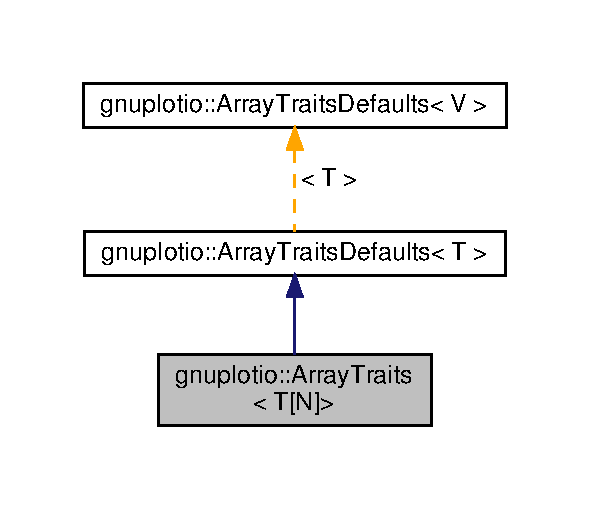
\includegraphics[width=283pt]{classgnuplotio_1_1_array_traits_3_01_t[_n]_4__inherit__graph}
\end{center}
\end{figure}


Collaboration diagram for gnuplotio\+:\+:Array\+Traits$<$ T\mbox{[}N\mbox{]}$>$\+:
\nopagebreak
\begin{figure}[H]
\begin{center}
\leavevmode
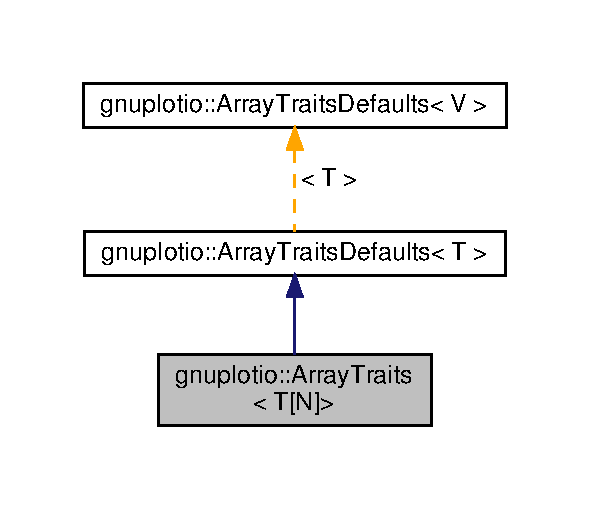
\includegraphics[width=283pt]{classgnuplotio_1_1_array_traits_3_01_t[_n]_4__coll__graph}
\end{center}
\end{figure}
\subsection*{Public Types}
\begin{DoxyCompactItemize}
\item 
typedef \hyperlink{classgnuplotio_1_1_iterator_range}{Iterator\+Range}$<$ const T $\ast$, T $>$ \hyperlink{classgnuplotio_1_1_array_traits_3_01_t[_n]_4_a926f3c3d14fbe82aab7b70ccc16d20fb}{range\+\_\+type}
\end{DoxyCompactItemize}
\subsection*{Static Public Member Functions}
\begin{DoxyCompactItemize}
\item 
static \hyperlink{classgnuplotio_1_1_array_traits_3_01_t[_n]_4_a926f3c3d14fbe82aab7b70ccc16d20fb}{range\+\_\+type} \hyperlink{classgnuplotio_1_1_array_traits_3_01_t[_n]_4_adc9c1ce6da4923418f367e08c150a928}{get\+\_\+range} (const T(\&arg)\mbox{[}N\mbox{]})
\end{DoxyCompactItemize}
\subsection*{Additional Inherited Members}


\subsection{Detailed Description}
\subsubsection*{template$<$typename T, size\+\_\+t N$>$\newline
class gnuplotio\+::\+Array\+Traits$<$ T\mbox{[}\+N\mbox{]}$>$}



Definition at line 913 of file gnuplot-\/iostream.\+h.



\subsection{Member Typedef Documentation}
\mbox{\Hypertarget{classgnuplotio_1_1_array_traits_3_01_t[_n]_4_a926f3c3d14fbe82aab7b70ccc16d20fb}\label{classgnuplotio_1_1_array_traits_3_01_t[_n]_4_a926f3c3d14fbe82aab7b70ccc16d20fb}} 
\index{gnuplotio\+::\+Array\+Traits$<$ T\mbox{[}N\mbox{]}$>$@{gnuplotio\+::\+Array\+Traits$<$ T[N]$>$}!range\+\_\+type@{range\+\_\+type}}
\index{range\+\_\+type@{range\+\_\+type}!gnuplotio\+::\+Array\+Traits$<$ T\mbox{[}N\mbox{]}$>$@{gnuplotio\+::\+Array\+Traits$<$ T[N]$>$}}
\subsubsection{\texorpdfstring{range\+\_\+type}{range\_type}}
{\footnotesize\ttfamily template$<$typename T , size\+\_\+t N$>$ \\
typedef \hyperlink{classgnuplotio_1_1_iterator_range}{Iterator\+Range}$<$const T$\ast$, T$>$ \hyperlink{classgnuplotio_1_1_array_traits}{gnuplotio\+::\+Array\+Traits}$<$ T\mbox{[}N\mbox{]}$>$\+::\hyperlink{classgnuplotio_1_1_array_traits_3_01_t[_n]_4_a926f3c3d14fbe82aab7b70ccc16d20fb}{range\+\_\+type}}



Definition at line 915 of file gnuplot-\/iostream.\+h.



\subsection{Member Function Documentation}
\mbox{\Hypertarget{classgnuplotio_1_1_array_traits_3_01_t[_n]_4_adc9c1ce6da4923418f367e08c150a928}\label{classgnuplotio_1_1_array_traits_3_01_t[_n]_4_adc9c1ce6da4923418f367e08c150a928}} 
\index{gnuplotio\+::\+Array\+Traits$<$ T\mbox{[}N\mbox{]}$>$@{gnuplotio\+::\+Array\+Traits$<$ T[N]$>$}!get\+\_\+range@{get\+\_\+range}}
\index{get\+\_\+range@{get\+\_\+range}!gnuplotio\+::\+Array\+Traits$<$ T\mbox{[}N\mbox{]}$>$@{gnuplotio\+::\+Array\+Traits$<$ T[N]$>$}}
\subsubsection{\texorpdfstring{get\+\_\+range()}{get\_range()}}
{\footnotesize\ttfamily template$<$typename T , size\+\_\+t N$>$ \\
static \hyperlink{classgnuplotio_1_1_array_traits_3_01_t[_n]_4_a926f3c3d14fbe82aab7b70ccc16d20fb}{range\+\_\+type} \hyperlink{classgnuplotio_1_1_array_traits}{gnuplotio\+::\+Array\+Traits}$<$ T\mbox{[}N\mbox{]}$>$\+::get\+\_\+range (\begin{DoxyParamCaption}\item[{const T(\&)}]{arg\mbox{[}\+N\mbox{]} }\end{DoxyParamCaption})\hspace{0.3cm}{\ttfamily [inline]}, {\ttfamily [static]}}



Definition at line 917 of file gnuplot-\/iostream.\+h.



The documentation for this class was generated from the following file\+:\begin{DoxyCompactItemize}
\item 
include/\hyperlink{gnuplot-iostream_8h}{gnuplot-\/iostream.\+h}\end{DoxyCompactItemize}

\hypertarget{classgnuplotio_1_1_array_traits_defaults}{}\section{gnuplotio\+:\+:Array\+Traits\+Defaults$<$ V $>$ Class Template Reference}
\label{classgnuplotio_1_1_array_traits_defaults}\index{gnuplotio\+::\+Array\+Traits\+Defaults$<$ V $>$@{gnuplotio\+::\+Array\+Traits\+Defaults$<$ V $>$}}


{\ttfamily \#include $<$gnuplot-\/iostream.\+h$>$}



Inheritance diagram for gnuplotio\+:\+:Array\+Traits\+Defaults$<$ V $>$\+:
\nopagebreak
\begin{figure}[H]
\begin{center}
\leavevmode
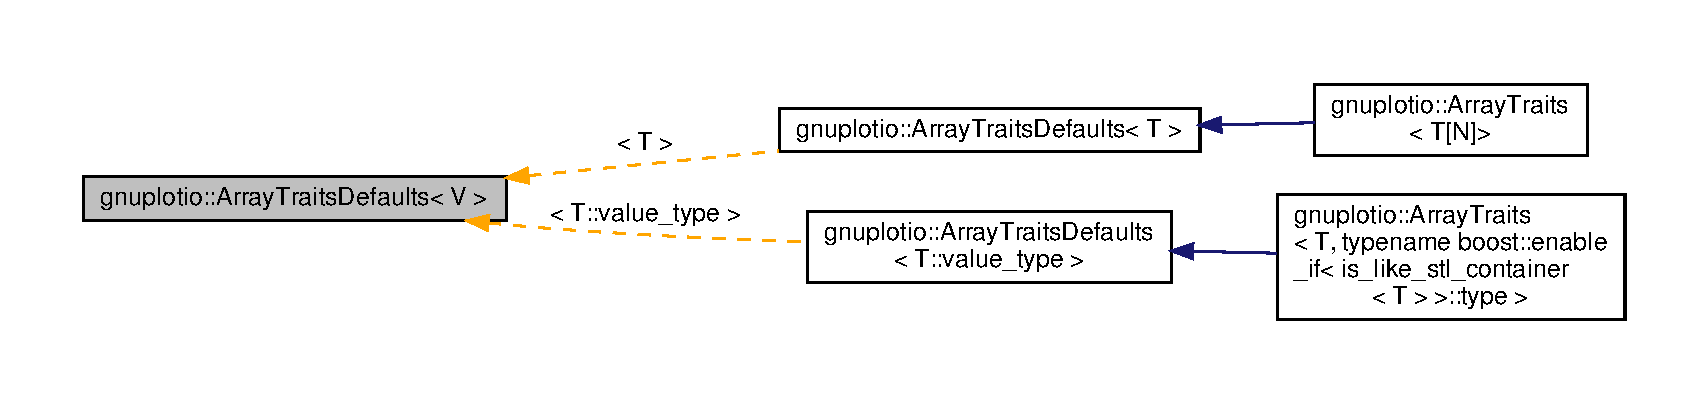
\includegraphics[width=350pt]{classgnuplotio_1_1_array_traits_defaults__inherit__graph}
\end{center}
\end{figure}
\subsection*{Public Types}
\begin{DoxyCompactItemize}
\item 
typedef V \hyperlink{classgnuplotio_1_1_array_traits_defaults_ad7a9e8d19419fabe2ab9cc1b76c9965b}{value\+\_\+type}
\end{DoxyCompactItemize}
\subsection*{Static Public Attributes}
\begin{DoxyCompactItemize}
\item 
static const bool \hyperlink{classgnuplotio_1_1_array_traits_defaults_a57bab5bf3617f0ee66fdd4dcb751aa21}{is\+\_\+container} = true
\item 
static const bool \hyperlink{classgnuplotio_1_1_array_traits_defaults_ac8d430cba6ceefc6f52706455f12a0e8}{allow\+\_\+auto\+\_\+unwrap} = true
\item 
static const size\+\_\+t \hyperlink{classgnuplotio_1_1_array_traits_defaults_ac51367f5da9096249b162af1496e36ab}{depth} = \hyperlink{classgnuplotio_1_1_array_traits}{Array\+Traits}$<$V$>$\+::depth + 1
\end{DoxyCompactItemize}


\subsection{Detailed Description}
\subsubsection*{template$<$typename V$>$\newline
class gnuplotio\+::\+Array\+Traits\+Defaults$<$ V $>$}



Definition at line 833 of file gnuplot-\/iostream.\+h.



\subsection{Member Typedef Documentation}
\mbox{\Hypertarget{classgnuplotio_1_1_array_traits_defaults_ad7a9e8d19419fabe2ab9cc1b76c9965b}\label{classgnuplotio_1_1_array_traits_defaults_ad7a9e8d19419fabe2ab9cc1b76c9965b}} 
\index{gnuplotio\+::\+Array\+Traits\+Defaults@{gnuplotio\+::\+Array\+Traits\+Defaults}!value\+\_\+type@{value\+\_\+type}}
\index{value\+\_\+type@{value\+\_\+type}!gnuplotio\+::\+Array\+Traits\+Defaults@{gnuplotio\+::\+Array\+Traits\+Defaults}}
\subsubsection{\texorpdfstring{value\+\_\+type}{value\_type}}
{\footnotesize\ttfamily template$<$typename V$>$ \\
typedef V \hyperlink{classgnuplotio_1_1_array_traits_defaults}{gnuplotio\+::\+Array\+Traits\+Defaults}$<$ V $>$\+::\hyperlink{classgnuplotio_1_1_array_traits_defaults_ad7a9e8d19419fabe2ab9cc1b76c9965b}{value\+\_\+type}}



Definition at line 835 of file gnuplot-\/iostream.\+h.



\subsection{Member Data Documentation}
\mbox{\Hypertarget{classgnuplotio_1_1_array_traits_defaults_ac8d430cba6ceefc6f52706455f12a0e8}\label{classgnuplotio_1_1_array_traits_defaults_ac8d430cba6ceefc6f52706455f12a0e8}} 
\index{gnuplotio\+::\+Array\+Traits\+Defaults@{gnuplotio\+::\+Array\+Traits\+Defaults}!allow\+\_\+auto\+\_\+unwrap@{allow\+\_\+auto\+\_\+unwrap}}
\index{allow\+\_\+auto\+\_\+unwrap@{allow\+\_\+auto\+\_\+unwrap}!gnuplotio\+::\+Array\+Traits\+Defaults@{gnuplotio\+::\+Array\+Traits\+Defaults}}
\subsubsection{\texorpdfstring{allow\+\_\+auto\+\_\+unwrap}{allow\_auto\_unwrap}}
{\footnotesize\ttfamily template$<$typename V$>$ \\
const bool \hyperlink{classgnuplotio_1_1_array_traits_defaults}{gnuplotio\+::\+Array\+Traits\+Defaults}$<$ V $>$\+::allow\+\_\+auto\+\_\+unwrap = true\hspace{0.3cm}{\ttfamily [static]}}



Definition at line 838 of file gnuplot-\/iostream.\+h.

\mbox{\Hypertarget{classgnuplotio_1_1_array_traits_defaults_ac51367f5da9096249b162af1496e36ab}\label{classgnuplotio_1_1_array_traits_defaults_ac51367f5da9096249b162af1496e36ab}} 
\index{gnuplotio\+::\+Array\+Traits\+Defaults@{gnuplotio\+::\+Array\+Traits\+Defaults}!depth@{depth}}
\index{depth@{depth}!gnuplotio\+::\+Array\+Traits\+Defaults@{gnuplotio\+::\+Array\+Traits\+Defaults}}
\subsubsection{\texorpdfstring{depth}{depth}}
{\footnotesize\ttfamily template$<$typename V$>$ \\
const size\+\_\+t \hyperlink{classgnuplotio_1_1_array_traits_defaults}{gnuplotio\+::\+Array\+Traits\+Defaults}$<$ V $>$\+::depth = \hyperlink{classgnuplotio_1_1_array_traits}{Array\+Traits}$<$V$>$\+::depth + 1\hspace{0.3cm}{\ttfamily [static]}}



Definition at line 839 of file gnuplot-\/iostream.\+h.

\mbox{\Hypertarget{classgnuplotio_1_1_array_traits_defaults_a57bab5bf3617f0ee66fdd4dcb751aa21}\label{classgnuplotio_1_1_array_traits_defaults_a57bab5bf3617f0ee66fdd4dcb751aa21}} 
\index{gnuplotio\+::\+Array\+Traits\+Defaults@{gnuplotio\+::\+Array\+Traits\+Defaults}!is\+\_\+container@{is\+\_\+container}}
\index{is\+\_\+container@{is\+\_\+container}!gnuplotio\+::\+Array\+Traits\+Defaults@{gnuplotio\+::\+Array\+Traits\+Defaults}}
\subsubsection{\texorpdfstring{is\+\_\+container}{is\_container}}
{\footnotesize\ttfamily template$<$typename V$>$ \\
const bool \hyperlink{classgnuplotio_1_1_array_traits_defaults}{gnuplotio\+::\+Array\+Traits\+Defaults}$<$ V $>$\+::is\+\_\+container = true\hspace{0.3cm}{\ttfamily [static]}}



Definition at line 837 of file gnuplot-\/iostream.\+h.



The documentation for this class was generated from the following file\+:\begin{DoxyCompactItemize}
\item 
include/\hyperlink{gnuplot-iostream_8h}{gnuplot-\/iostream.\+h}\end{DoxyCompactItemize}

\hypertarget{structgnuplotio_1_1_binary_sender}{}\section{gnuplotio\+:\+:Binary\+Sender$<$ T, Enable $>$ Struct Template Reference}
\label{structgnuplotio_1_1_binary_sender}\index{gnuplotio\+::\+Binary\+Sender$<$ T, Enable $>$@{gnuplotio\+::\+Binary\+Sender$<$ T, Enable $>$}}


{\ttfamily \#include $<$gnuplot-\/iostream.\+h$>$}

\subsection*{Public Member Functions}
\begin{DoxyCompactItemize}
\item 
\hyperlink{structgnuplotio_1_1_binary_sender_ad964fa720473ff517cfb461361f645c8}{G\+N\+U\+P\+L\+O\+T\+\_\+\+S\+T\+A\+T\+I\+C\+\_\+\+A\+S\+S\+E\+R\+T\+\_\+\+M\+SG} ((sizeof(T)==0), \char`\"{}Binary\+Sender class not specialized for this type\char`\"{})
\end{DoxyCompactItemize}
\subsection*{Static Public Member Functions}
\begin{DoxyCompactItemize}
\item 
static void \hyperlink{structgnuplotio_1_1_binary_sender_a4b5dd22b7679c4f0ce4d8e75b36c8a21}{send} (std\+::ostream \&stream, const T \&v)
\end{DoxyCompactItemize}


\subsection{Detailed Description}
\subsubsection*{template$<$typename T, typename Enable = void$>$\newline
struct gnuplotio\+::\+Binary\+Sender$<$ T, Enable $>$}



Definition at line 441 of file gnuplot-\/iostream.\+h.



\subsection{Member Function Documentation}
\mbox{\Hypertarget{structgnuplotio_1_1_binary_sender_ad964fa720473ff517cfb461361f645c8}\label{structgnuplotio_1_1_binary_sender_ad964fa720473ff517cfb461361f645c8}} 
\index{gnuplotio\+::\+Binary\+Sender@{gnuplotio\+::\+Binary\+Sender}!G\+N\+U\+P\+L\+O\+T\+\_\+\+S\+T\+A\+T\+I\+C\+\_\+\+A\+S\+S\+E\+R\+T\+\_\+\+M\+SG@{G\+N\+U\+P\+L\+O\+T\+\_\+\+S\+T\+A\+T\+I\+C\+\_\+\+A\+S\+S\+E\+R\+T\+\_\+\+M\+SG}}
\index{G\+N\+U\+P\+L\+O\+T\+\_\+\+S\+T\+A\+T\+I\+C\+\_\+\+A\+S\+S\+E\+R\+T\+\_\+\+M\+SG@{G\+N\+U\+P\+L\+O\+T\+\_\+\+S\+T\+A\+T\+I\+C\+\_\+\+A\+S\+S\+E\+R\+T\+\_\+\+M\+SG}!gnuplotio\+::\+Binary\+Sender@{gnuplotio\+::\+Binary\+Sender}}
\subsubsection{\texorpdfstring{G\+N\+U\+P\+L\+O\+T\+\_\+\+S\+T\+A\+T\+I\+C\+\_\+\+A\+S\+S\+E\+R\+T\+\_\+\+M\+S\+G()}{GNUPLOT\_STATIC\_ASSERT\_MSG()}}
{\footnotesize\ttfamily template$<$typename T, typename Enable = void$>$ \\
\hyperlink{structgnuplotio_1_1_binary_sender}{gnuplotio\+::\+Binary\+Sender}$<$ T, Enable $>$\+::G\+N\+U\+P\+L\+O\+T\+\_\+\+S\+T\+A\+T\+I\+C\+\_\+\+A\+S\+S\+E\+R\+T\+\_\+\+M\+SG (\begin{DoxyParamCaption}\item[{(sizeof(T)==0)}]{,  }\item[{\char`\"{}Binary\+Sender$<$ T, Enable $>$ class not specialized for this type\char`\"{}}]{ }\end{DoxyParamCaption})}

\mbox{\Hypertarget{structgnuplotio_1_1_binary_sender_a4b5dd22b7679c4f0ce4d8e75b36c8a21}\label{structgnuplotio_1_1_binary_sender_a4b5dd22b7679c4f0ce4d8e75b36c8a21}} 
\index{gnuplotio\+::\+Binary\+Sender@{gnuplotio\+::\+Binary\+Sender}!send@{send}}
\index{send@{send}!gnuplotio\+::\+Binary\+Sender@{gnuplotio\+::\+Binary\+Sender}}
\subsubsection{\texorpdfstring{send()}{send()}}
{\footnotesize\ttfamily template$<$typename T, typename Enable = void$>$ \\
static void \hyperlink{structgnuplotio_1_1_binary_sender}{gnuplotio\+::\+Binary\+Sender}$<$ T, Enable $>$\+::send (\begin{DoxyParamCaption}\item[{std\+::ostream \&}]{stream,  }\item[{const T \&}]{v }\end{DoxyParamCaption})\hspace{0.3cm}{\ttfamily [static]}}



Referenced by gnuplotio\+::\+Binary\+Sender$<$ std\+::pair$<$ T, U $>$ $>$\+::send(), gnuplotio\+::\+Binary\+Sender$<$ std\+::complex$<$ T $>$ $>$\+::send(), gnuplotio\+::\+Binary\+Sender$<$ T, typename boost\+::enable\+\_\+if$<$ boost\+::mpl\+::and\+\_\+$<$ is\+\_\+boost\+\_\+tuple$<$ T $>$, boost\+::mpl\+::not\+\_\+$<$ is\+\_\+boost\+\_\+tuple\+\_\+nulltype$<$ typename T\+::tail\+\_\+type $>$ $>$ $>$ $>$\+::type $>$\+::send(), gnuplotio\+::\+Binary\+Sender$<$ T, typename boost\+::enable\+\_\+if$<$ boost\+::mpl\+::and\+\_\+$<$ is\+\_\+boost\+\_\+tuple$<$ T $>$, is\+\_\+boost\+\_\+tuple\+\_\+nulltype$<$ typename T\+::tail\+\_\+type $>$ $>$ $>$\+::type $>$\+::send(), and gnuplotio\+::send\+\_\+scalar().



The documentation for this struct was generated from the following file\+:\begin{DoxyCompactItemize}
\item 
include/\hyperlink{gnuplot-iostream_8h}{gnuplot-\/iostream.\+h}\end{DoxyCompactItemize}

\hypertarget{structgnuplotio_1_1_binary_sender_3_01boost_1_1int16__t_01_4}{}\doxysection{gnuplotio\+::Binary\+Sender$<$ boost\+::int16\+\_\+t $>$ Struct Reference}
\label{structgnuplotio_1_1_binary_sender_3_01boost_1_1int16__t_01_4}\index{gnuplotio::BinarySender$<$ boost::int16\_t $>$@{gnuplotio::BinarySender$<$ boost::int16\_t $>$}}


{\ttfamily \#include $<$gnuplot-\/iostream.\+h$>$}



Inheritance diagram for gnuplotio\+::Binary\+Sender$<$ boost\+::int16\+\_\+t $>$\+:\nopagebreak
\begin{figure}[H]
\begin{center}
\leavevmode
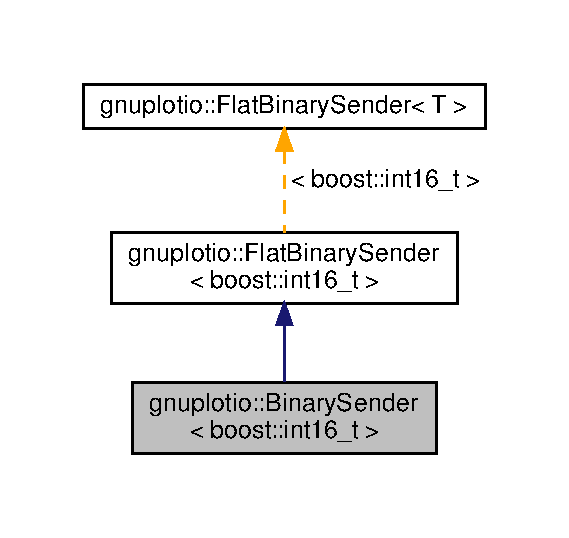
\includegraphics[width=301pt]{structgnuplotio_1_1_binary_sender_3_01boost_1_1int16__t_01_4__inherit__graph}
\end{center}
\end{figure}


Collaboration diagram for gnuplotio\+::Binary\+Sender$<$ boost\+::int16\+\_\+t $>$\+:\nopagebreak
\begin{figure}[H]
\begin{center}
\leavevmode
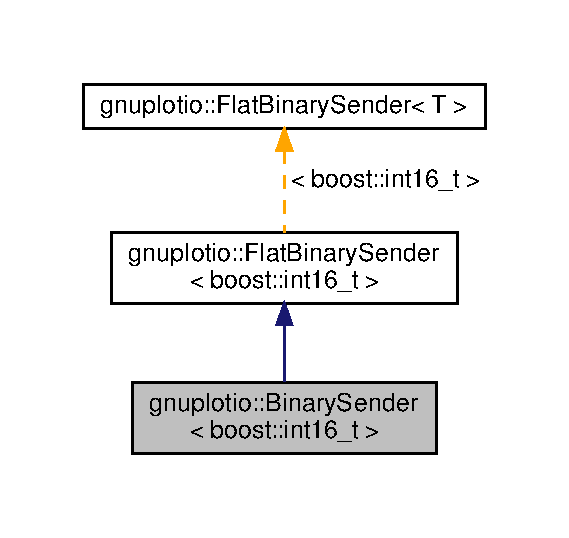
\includegraphics[width=301pt]{structgnuplotio_1_1_binary_sender_3_01boost_1_1int16__t_01_4__coll__graph}
\end{center}
\end{figure}
\doxysubsection*{Additional Inherited Members}


\doxysubsection{Detailed Description}


Definition at line 485 of file gnuplot-\/iostream.\+h.



The documentation for this struct was generated from the following file\+:\begin{DoxyCompactItemize}
\item 
/home/adev/\+Documents/\+S\+T\+E\+C\+H/stewart\+\_\+platform/include/\mbox{\hyperlink{gnuplot-iostream_8h}{gnuplot-\/iostream.\+h}}\end{DoxyCompactItemize}

\hypertarget{structgnuplotio_1_1_binary_sender_3_01boost_1_1int32__t_01_4}{}\section{gnuplotio\+:\+:Binary\+Sender$<$ boost\+:\+:int32\+\_\+t $>$ Struct Template Reference}
\label{structgnuplotio_1_1_binary_sender_3_01boost_1_1int32__t_01_4}\index{gnuplotio\+::\+Binary\+Sender$<$ boost\+::int32\+\_\+t $>$@{gnuplotio\+::\+Binary\+Sender$<$ boost\+::int32\+\_\+t $>$}}


{\ttfamily \#include $<$gnuplot-\/iostream.\+h$>$}



Inheritance diagram for gnuplotio\+:\+:Binary\+Sender$<$ boost\+:\+:int32\+\_\+t $>$\+:
\nopagebreak
\begin{figure}[H]
\begin{center}
\leavevmode
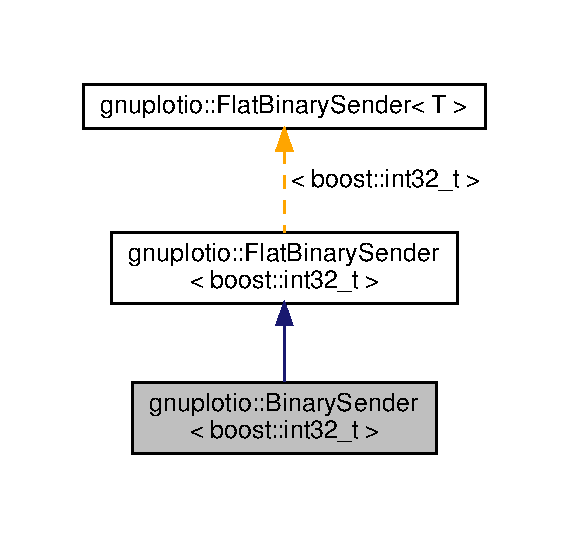
\includegraphics[width=273pt]{structgnuplotio_1_1_binary_sender_3_01boost_1_1int32__t_01_4__inherit__graph}
\end{center}
\end{figure}


Collaboration diagram for gnuplotio\+:\+:Binary\+Sender$<$ boost\+:\+:int32\+\_\+t $>$\+:
\nopagebreak
\begin{figure}[H]
\begin{center}
\leavevmode
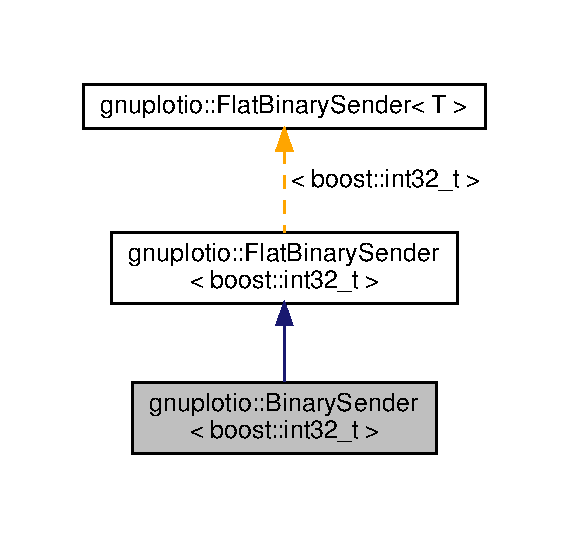
\includegraphics[width=273pt]{structgnuplotio_1_1_binary_sender_3_01boost_1_1int32__t_01_4__coll__graph}
\end{center}
\end{figure}
\subsection*{Additional Inherited Members}


\subsection{Detailed Description}
\subsubsection*{template$<$$>$\newline
struct gnuplotio\+::\+Binary\+Sender$<$ boost\+::int32\+\_\+t $>$}



Definition at line 487 of file gnuplot-\/iostream.\+h.



The documentation for this struct was generated from the following file\+:\begin{DoxyCompactItemize}
\item 
include/\hyperlink{gnuplot-iostream_8h}{gnuplot-\/iostream.\+h}\end{DoxyCompactItemize}

\hypertarget{structgnuplotio_1_1_binary_sender_3_01boost_1_1int64__t_01_4}{}\section{gnuplotio\+:\+:Binary\+Sender$<$ boost\+:\+:int64\+\_\+t $>$ Struct Template Reference}
\label{structgnuplotio_1_1_binary_sender_3_01boost_1_1int64__t_01_4}\index{gnuplotio\+::\+Binary\+Sender$<$ boost\+::int64\+\_\+t $>$@{gnuplotio\+::\+Binary\+Sender$<$ boost\+::int64\+\_\+t $>$}}


{\ttfamily \#include $<$gnuplot-\/iostream.\+h$>$}



Inheritance diagram for gnuplotio\+:\+:Binary\+Sender$<$ boost\+:\+:int64\+\_\+t $>$\+:
\nopagebreak
\begin{figure}[H]
\begin{center}
\leavevmode
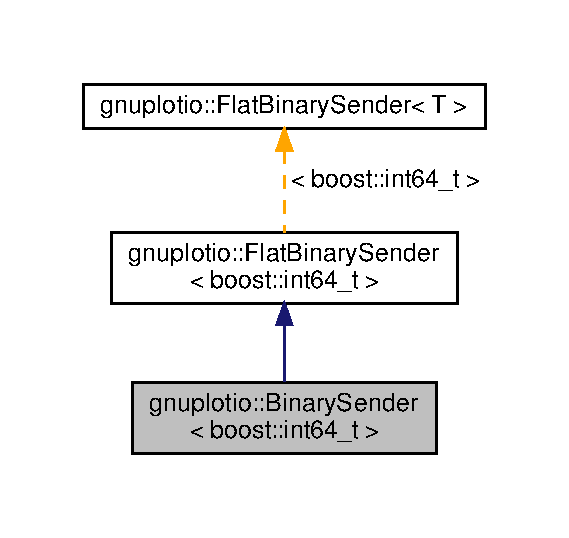
\includegraphics[width=273pt]{structgnuplotio_1_1_binary_sender_3_01boost_1_1int64__t_01_4__inherit__graph}
\end{center}
\end{figure}


Collaboration diagram for gnuplotio\+:\+:Binary\+Sender$<$ boost\+:\+:int64\+\_\+t $>$\+:
\nopagebreak
\begin{figure}[H]
\begin{center}
\leavevmode
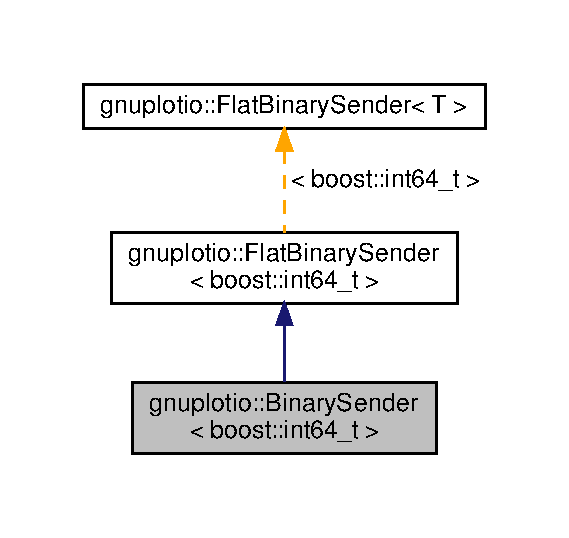
\includegraphics[width=273pt]{structgnuplotio_1_1_binary_sender_3_01boost_1_1int64__t_01_4__coll__graph}
\end{center}
\end{figure}
\subsection*{Additional Inherited Members}


\subsection{Detailed Description}
\subsubsection*{template$<$$>$\newline
struct gnuplotio\+::\+Binary\+Sender$<$ boost\+::int64\+\_\+t $>$}



Definition at line 489 of file gnuplot-\/iostream.\+h.



The documentation for this struct was generated from the following file\+:\begin{DoxyCompactItemize}
\item 
include/\hyperlink{gnuplot-iostream_8h}{gnuplot-\/iostream.\+h}\end{DoxyCompactItemize}

\hypertarget{structgnuplotio_1_1_binary_sender_3_01boost_1_1int8__t_01_4}{}\doxysection{gnuplotio\+::Binary\+Sender$<$ boost\+::int8\+\_\+t $>$ Struct Reference}
\label{structgnuplotio_1_1_binary_sender_3_01boost_1_1int8__t_01_4}\index{gnuplotio::BinarySender$<$ boost::int8\_t $>$@{gnuplotio::BinarySender$<$ boost::int8\_t $>$}}


{\ttfamily \#include $<$gnuplot-\/iostream.\+h$>$}



Inheritance diagram for gnuplotio\+::Binary\+Sender$<$ boost\+::int8\+\_\+t $>$\+:\nopagebreak
\begin{figure}[H]
\begin{center}
\leavevmode
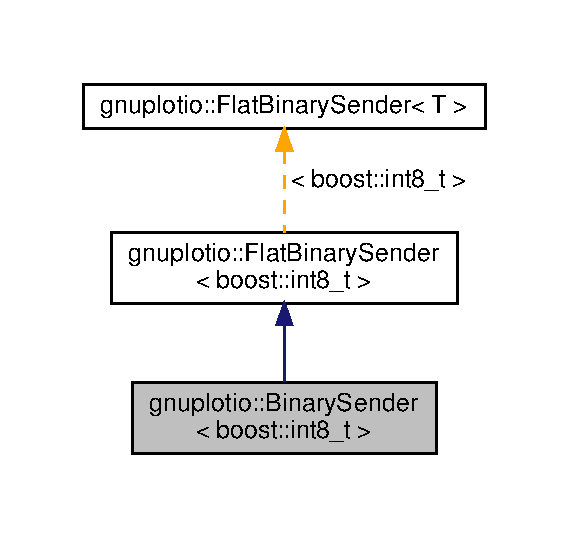
\includegraphics[width=297pt]{structgnuplotio_1_1_binary_sender_3_01boost_1_1int8__t_01_4__inherit__graph}
\end{center}
\end{figure}


Collaboration diagram for gnuplotio\+::Binary\+Sender$<$ boost\+::int8\+\_\+t $>$\+:\nopagebreak
\begin{figure}[H]
\begin{center}
\leavevmode
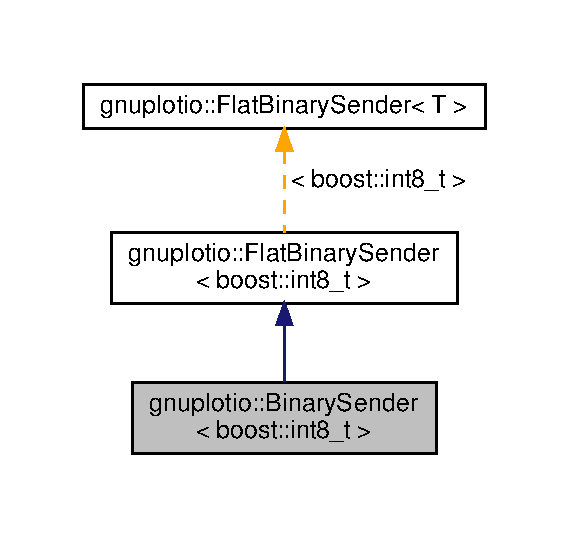
\includegraphics[width=297pt]{structgnuplotio_1_1_binary_sender_3_01boost_1_1int8__t_01_4__coll__graph}
\end{center}
\end{figure}
\doxysubsection*{Additional Inherited Members}


\doxysubsection{Detailed Description}


Definition at line 483 of file gnuplot-\/iostream.\+h.



The documentation for this struct was generated from the following file\+:\begin{DoxyCompactItemize}
\item 
/home/adev/\+Documents/\+S\+T\+E\+C\+H/stewart\+\_\+platform/include/\mbox{\hyperlink{gnuplot-iostream_8h}{gnuplot-\/iostream.\+h}}\end{DoxyCompactItemize}

\hypertarget{structgnuplotio_1_1_binary_sender_3_01boost_1_1uint16__t_01_4}{}\section{gnuplotio\+:\+:Binary\+Sender$<$ boost\+:\+:uint16\+\_\+t $>$ Struct Template Reference}
\label{structgnuplotio_1_1_binary_sender_3_01boost_1_1uint16__t_01_4}\index{gnuplotio\+::\+Binary\+Sender$<$ boost\+::uint16\+\_\+t $>$@{gnuplotio\+::\+Binary\+Sender$<$ boost\+::uint16\+\_\+t $>$}}


{\ttfamily \#include $<$gnuplot-\/iostream.\+h$>$}



Inheritance diagram for gnuplotio\+:\+:Binary\+Sender$<$ boost\+:\+:uint16\+\_\+t $>$\+:
\nopagebreak
\begin{figure}[H]
\begin{center}
\leavevmode
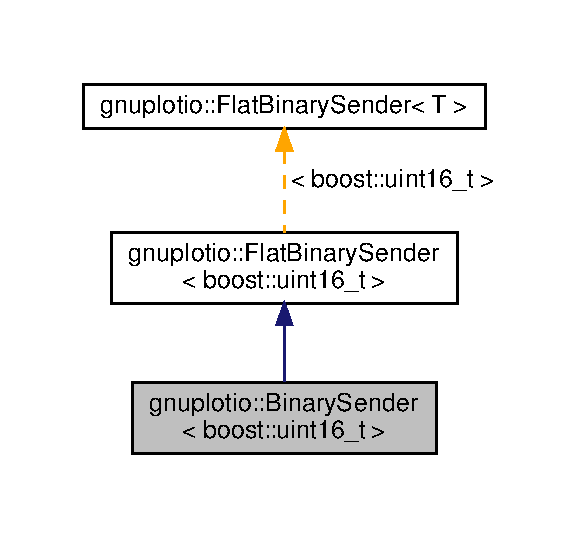
\includegraphics[width=278pt]{structgnuplotio_1_1_binary_sender_3_01boost_1_1uint16__t_01_4__inherit__graph}
\end{center}
\end{figure}


Collaboration diagram for gnuplotio\+:\+:Binary\+Sender$<$ boost\+:\+:uint16\+\_\+t $>$\+:
\nopagebreak
\begin{figure}[H]
\begin{center}
\leavevmode
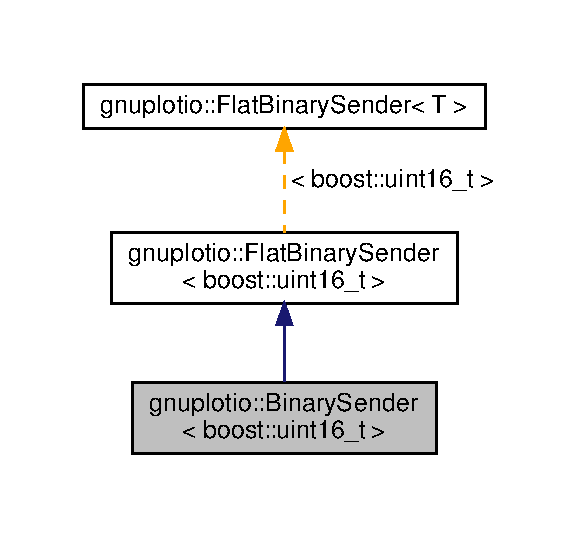
\includegraphics[width=278pt]{structgnuplotio_1_1_binary_sender_3_01boost_1_1uint16__t_01_4__coll__graph}
\end{center}
\end{figure}
\subsection*{Additional Inherited Members}


\subsection{Detailed Description}
\subsubsection*{template$<$$>$\newline
struct gnuplotio\+::\+Binary\+Sender$<$ boost\+::uint16\+\_\+t $>$}



Definition at line 486 of file gnuplot-\/iostream.\+h.



The documentation for this struct was generated from the following file\+:\begin{DoxyCompactItemize}
\item 
include/\hyperlink{gnuplot-iostream_8h}{gnuplot-\/iostream.\+h}\end{DoxyCompactItemize}

\hypertarget{structgnuplotio_1_1_binary_sender_3_01boost_1_1uint32__t_01_4}{}\doxysection{gnuplotio\+::Binary\+Sender$<$ boost\+::uint32\+\_\+t $>$ Struct Reference}
\label{structgnuplotio_1_1_binary_sender_3_01boost_1_1uint32__t_01_4}\index{gnuplotio::BinarySender$<$ boost::uint32\_t $>$@{gnuplotio::BinarySender$<$ boost::uint32\_t $>$}}


{\ttfamily \#include $<$gnuplot-\/iostream.\+h$>$}



Inheritance diagram for gnuplotio\+::Binary\+Sender$<$ boost\+::uint32\+\_\+t $>$\+:\nopagebreak
\begin{figure}[H]
\begin{center}
\leavevmode
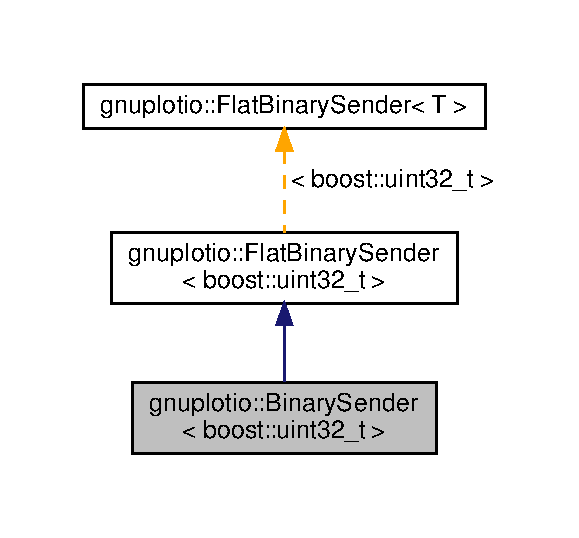
\includegraphics[width=309pt]{structgnuplotio_1_1_binary_sender_3_01boost_1_1uint32__t_01_4__inherit__graph}
\end{center}
\end{figure}


Collaboration diagram for gnuplotio\+::Binary\+Sender$<$ boost\+::uint32\+\_\+t $>$\+:\nopagebreak
\begin{figure}[H]
\begin{center}
\leavevmode
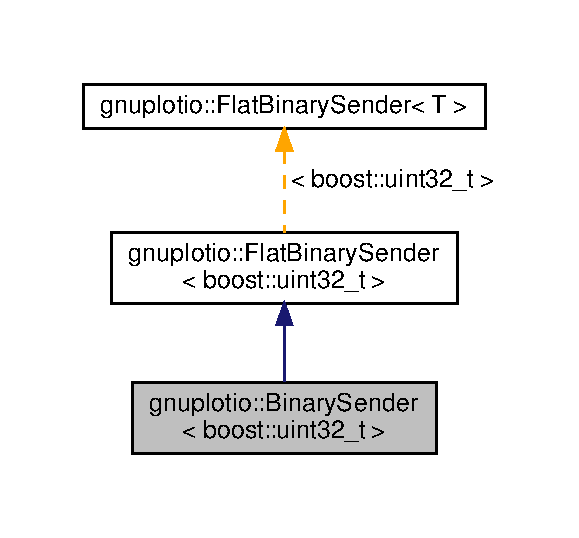
\includegraphics[width=309pt]{structgnuplotio_1_1_binary_sender_3_01boost_1_1uint32__t_01_4__coll__graph}
\end{center}
\end{figure}
\doxysubsection*{Additional Inherited Members}


\doxysubsection{Detailed Description}


Definition at line 488 of file gnuplot-\/iostream.\+h.



The documentation for this struct was generated from the following file\+:\begin{DoxyCompactItemize}
\item 
/home/adev/\+Documents/\+S\+T\+E\+C\+H/stewart\+\_\+platform/include/\mbox{\hyperlink{gnuplot-iostream_8h}{gnuplot-\/iostream.\+h}}\end{DoxyCompactItemize}

\hypertarget{structgnuplotio_1_1_binary_sender_3_01boost_1_1uint64__t_01_4}{}\doxysection{gnuplotio\+::Binary\+Sender$<$ boost\+::uint64\+\_\+t $>$ Struct Reference}
\label{structgnuplotio_1_1_binary_sender_3_01boost_1_1uint64__t_01_4}\index{gnuplotio::BinarySender$<$ boost::uint64\_t $>$@{gnuplotio::BinarySender$<$ boost::uint64\_t $>$}}


{\ttfamily \#include $<$gnuplot-\/iostream.\+h$>$}



Inheritance diagram for gnuplotio\+::Binary\+Sender$<$ boost\+::uint64\+\_\+t $>$\+:\nopagebreak
\begin{figure}[H]
\begin{center}
\leavevmode
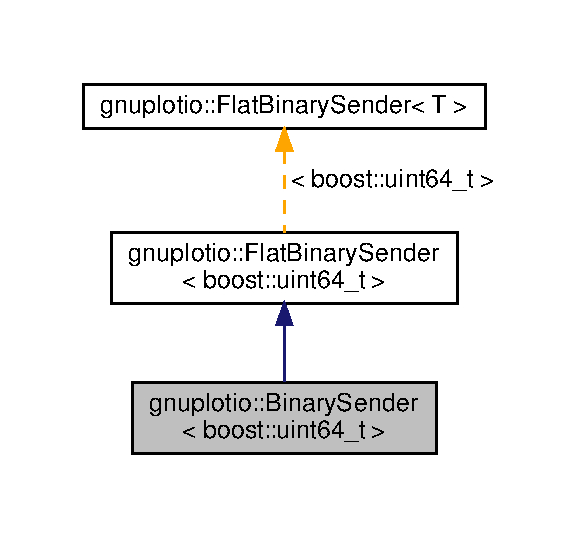
\includegraphics[width=309pt]{structgnuplotio_1_1_binary_sender_3_01boost_1_1uint64__t_01_4__inherit__graph}
\end{center}
\end{figure}


Collaboration diagram for gnuplotio\+::Binary\+Sender$<$ boost\+::uint64\+\_\+t $>$\+:\nopagebreak
\begin{figure}[H]
\begin{center}
\leavevmode
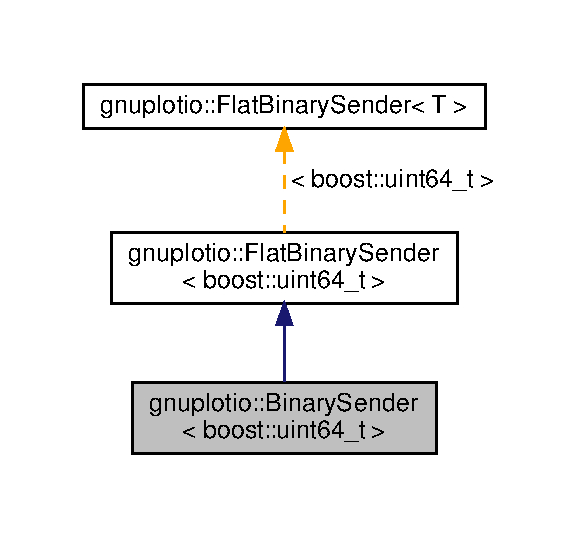
\includegraphics[width=309pt]{structgnuplotio_1_1_binary_sender_3_01boost_1_1uint64__t_01_4__coll__graph}
\end{center}
\end{figure}
\doxysubsection*{Additional Inherited Members}


\doxysubsection{Detailed Description}


Definition at line 490 of file gnuplot-\/iostream.\+h.



The documentation for this struct was generated from the following file\+:\begin{DoxyCompactItemize}
\item 
/home/adev/\+Documents/\+S\+T\+E\+C\+H/stewart\+\_\+platform/include/\mbox{\hyperlink{gnuplot-iostream_8h}{gnuplot-\/iostream.\+h}}\end{DoxyCompactItemize}

\hypertarget{structgnuplotio_1_1_binary_sender_3_01boost_1_1uint8__t_01_4}{}\section{gnuplotio\+:\+:Binary\+Sender$<$ boost\+:\+:uint8\+\_\+t $>$ Struct Template Reference}
\label{structgnuplotio_1_1_binary_sender_3_01boost_1_1uint8__t_01_4}\index{gnuplotio\+::\+Binary\+Sender$<$ boost\+::uint8\+\_\+t $>$@{gnuplotio\+::\+Binary\+Sender$<$ boost\+::uint8\+\_\+t $>$}}


{\ttfamily \#include $<$gnuplot-\/iostream.\+h$>$}



Inheritance diagram for gnuplotio\+:\+:Binary\+Sender$<$ boost\+:\+:uint8\+\_\+t $>$\+:
\nopagebreak
\begin{figure}[H]
\begin{center}
\leavevmode
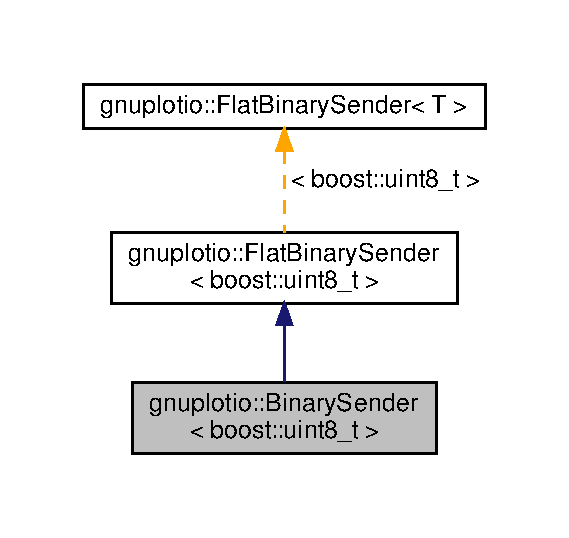
\includegraphics[width=273pt]{structgnuplotio_1_1_binary_sender_3_01boost_1_1uint8__t_01_4__inherit__graph}
\end{center}
\end{figure}


Collaboration diagram for gnuplotio\+:\+:Binary\+Sender$<$ boost\+:\+:uint8\+\_\+t $>$\+:
\nopagebreak
\begin{figure}[H]
\begin{center}
\leavevmode
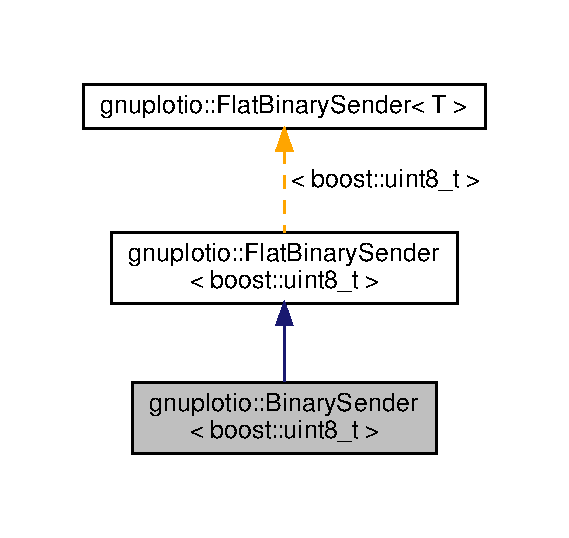
\includegraphics[width=273pt]{structgnuplotio_1_1_binary_sender_3_01boost_1_1uint8__t_01_4__coll__graph}
\end{center}
\end{figure}
\subsection*{Additional Inherited Members}


\subsection{Detailed Description}
\subsubsection*{template$<$$>$\newline
struct gnuplotio\+::\+Binary\+Sender$<$ boost\+::uint8\+\_\+t $>$}



Definition at line 484 of file gnuplot-\/iostream.\+h.



The documentation for this struct was generated from the following file\+:\begin{DoxyCompactItemize}
\item 
include/\hyperlink{gnuplot-iostream_8h}{gnuplot-\/iostream.\+h}\end{DoxyCompactItemize}

\hypertarget{structgnuplotio_1_1_binary_sender_3_01double_01_4}{}\doxysection{gnuplotio\+::Binary\+Sender$<$ double $>$ Struct Reference}
\label{structgnuplotio_1_1_binary_sender_3_01double_01_4}\index{gnuplotio::BinarySender$<$ double $>$@{gnuplotio::BinarySender$<$ double $>$}}


{\ttfamily \#include $<$gnuplot-\/iostream.\+h$>$}



Inheritance diagram for gnuplotio\+::Binary\+Sender$<$ double $>$\+:\nopagebreak
\begin{figure}[H]
\begin{center}
\leavevmode
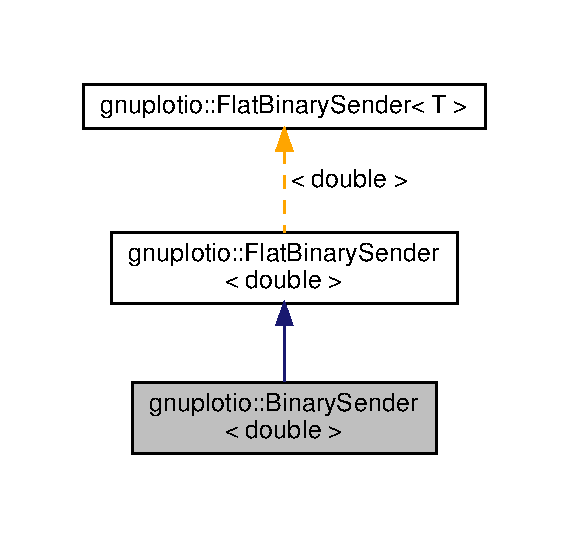
\includegraphics[width=297pt]{structgnuplotio_1_1_binary_sender_3_01double_01_4__inherit__graph}
\end{center}
\end{figure}


Collaboration diagram for gnuplotio\+::Binary\+Sender$<$ double $>$\+:\nopagebreak
\begin{figure}[H]
\begin{center}
\leavevmode
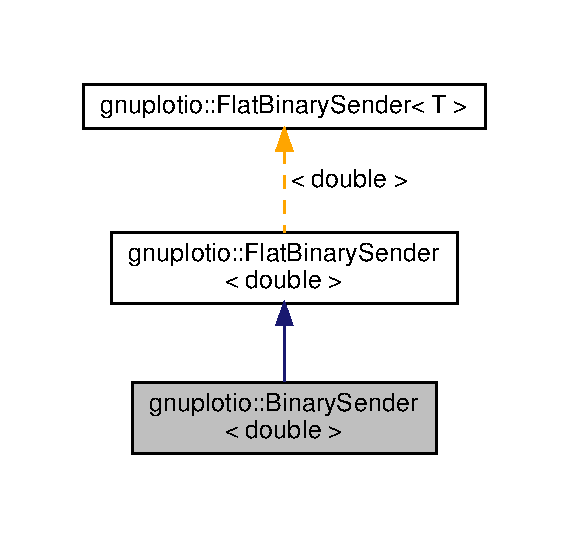
\includegraphics[width=297pt]{structgnuplotio_1_1_binary_sender_3_01double_01_4__coll__graph}
\end{center}
\end{figure}
\doxysubsection*{Additional Inherited Members}


\doxysubsection{Detailed Description}


Definition at line 482 of file gnuplot-\/iostream.\+h.



The documentation for this struct was generated from the following file\+:\begin{DoxyCompactItemize}
\item 
/home/adev/\+Documents/\+S\+T\+E\+C\+H/stewart\+\_\+platform/include/\mbox{\hyperlink{gnuplot-iostream_8h}{gnuplot-\/iostream.\+h}}\end{DoxyCompactItemize}

\hypertarget{structgnuplotio_1_1_binary_sender_3_01float_01_4}{}\section{gnuplotio\+:\+:Binary\+Sender$<$ float $>$ Struct Template Reference}
\label{structgnuplotio_1_1_binary_sender_3_01float_01_4}\index{gnuplotio\+::\+Binary\+Sender$<$ float $>$@{gnuplotio\+::\+Binary\+Sender$<$ float $>$}}


{\ttfamily \#include $<$gnuplot-\/iostream.\+h$>$}



Inheritance diagram for gnuplotio\+:\+:Binary\+Sender$<$ float $>$\+:
\nopagebreak
\begin{figure}[H]
\begin{center}
\leavevmode
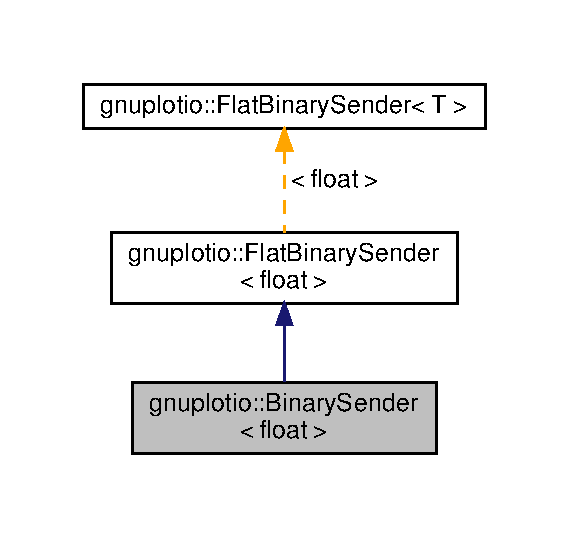
\includegraphics[width=273pt]{structgnuplotio_1_1_binary_sender_3_01float_01_4__inherit__graph}
\end{center}
\end{figure}


Collaboration diagram for gnuplotio\+:\+:Binary\+Sender$<$ float $>$\+:
\nopagebreak
\begin{figure}[H]
\begin{center}
\leavevmode
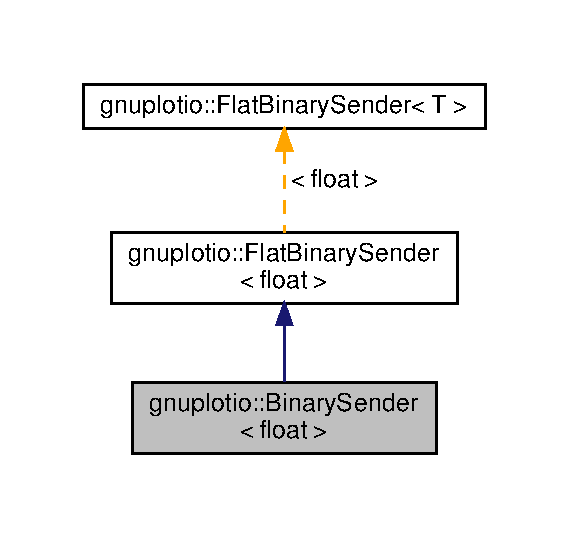
\includegraphics[width=273pt]{structgnuplotio_1_1_binary_sender_3_01float_01_4__coll__graph}
\end{center}
\end{figure}
\subsection*{Additional Inherited Members}


\subsection{Detailed Description}
\subsubsection*{template$<$$>$\newline
struct gnuplotio\+::\+Binary\+Sender$<$ float $>$}



Definition at line 481 of file gnuplot-\/iostream.\+h.



The documentation for this struct was generated from the following file\+:\begin{DoxyCompactItemize}
\item 
include/\hyperlink{gnuplot-iostream_8h}{gnuplot-\/iostream.\+h}\end{DoxyCompactItemize}

\hypertarget{structgnuplotio_1_1_binary_sender_3_01std_1_1complex_3_01_t_01_4_01_4}{}\section{gnuplotio\+:\+:Binary\+Sender$<$ std\+:\+:complex$<$ T $>$ $>$ Struct Template Reference}
\label{structgnuplotio_1_1_binary_sender_3_01std_1_1complex_3_01_t_01_4_01_4}\index{gnuplotio\+::\+Binary\+Sender$<$ std\+::complex$<$ T $>$ $>$@{gnuplotio\+::\+Binary\+Sender$<$ std\+::complex$<$ T $>$ $>$}}


{\ttfamily \#include $<$gnuplot-\/iostream.\+h$>$}

\subsection*{Static Public Member Functions}
\begin{DoxyCompactItemize}
\item 
static void \hyperlink{structgnuplotio_1_1_binary_sender_3_01std_1_1complex_3_01_t_01_4_01_4_a759de700a1cd68000830a4b15a6fec49}{send} (std\+::ostream \&stream, const std\+::complex$<$ T $>$ \&v)
\end{DoxyCompactItemize}


\subsection{Detailed Description}
\subsubsection*{template$<$typename T$>$\newline
struct gnuplotio\+::\+Binary\+Sender$<$ std\+::complex$<$ T $>$ $>$}



Definition at line 565 of file gnuplot-\/iostream.\+h.



\subsection{Member Function Documentation}
\mbox{\Hypertarget{structgnuplotio_1_1_binary_sender_3_01std_1_1complex_3_01_t_01_4_01_4_a759de700a1cd68000830a4b15a6fec49}\label{structgnuplotio_1_1_binary_sender_3_01std_1_1complex_3_01_t_01_4_01_4_a759de700a1cd68000830a4b15a6fec49}} 
\index{gnuplotio\+::\+Binary\+Sender$<$ std\+::complex$<$ T $>$ $>$@{gnuplotio\+::\+Binary\+Sender$<$ std\+::complex$<$ T $>$ $>$}!send@{send}}
\index{send@{send}!gnuplotio\+::\+Binary\+Sender$<$ std\+::complex$<$ T $>$ $>$@{gnuplotio\+::\+Binary\+Sender$<$ std\+::complex$<$ T $>$ $>$}}
\subsubsection{\texorpdfstring{send()}{send()}}
{\footnotesize\ttfamily template$<$typename T $>$ \\
static void \hyperlink{structgnuplotio_1_1_binary_sender}{gnuplotio\+::\+Binary\+Sender}$<$ std\+::complex$<$ T $>$ $>$\+::send (\begin{DoxyParamCaption}\item[{std\+::ostream \&}]{stream,  }\item[{const std\+::complex$<$ T $>$ \&}]{v }\end{DoxyParamCaption})\hspace{0.3cm}{\ttfamily [inline]}, {\ttfamily [static]}}



Definition at line 566 of file gnuplot-\/iostream.\+h.



References gnuplotio\+::\+Binary\+Sender$<$ T, Enable $>$\+::send().

Here is the call graph for this function\+:\nopagebreak
\begin{figure}[H]
\begin{center}
\leavevmode
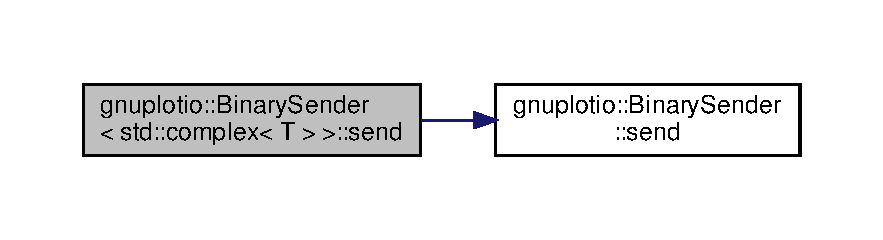
\includegraphics[width=350pt]{structgnuplotio_1_1_binary_sender_3_01std_1_1complex_3_01_t_01_4_01_4_a759de700a1cd68000830a4b15a6fec49_cgraph}
\end{center}
\end{figure}


The documentation for this struct was generated from the following file\+:\begin{DoxyCompactItemize}
\item 
include/\hyperlink{gnuplot-iostream_8h}{gnuplot-\/iostream.\+h}\end{DoxyCompactItemize}

\hypertarget{structgnuplotio_1_1_binary_sender_3_01std_1_1pair_3_01_t_00_01_u_01_4_01_4}{}\section{gnuplotio\+:\+:Binary\+Sender$<$ std\+:\+:pair$<$ T, U $>$ $>$ Struct Template Reference}
\label{structgnuplotio_1_1_binary_sender_3_01std_1_1pair_3_01_t_00_01_u_01_4_01_4}\index{gnuplotio\+::\+Binary\+Sender$<$ std\+::pair$<$ T, U $>$ $>$@{gnuplotio\+::\+Binary\+Sender$<$ std\+::pair$<$ T, U $>$ $>$}}


{\ttfamily \#include $<$gnuplot-\/iostream.\+h$>$}

\subsection*{Static Public Member Functions}
\begin{DoxyCompactItemize}
\item 
static void \hyperlink{structgnuplotio_1_1_binary_sender_3_01std_1_1pair_3_01_t_00_01_u_01_4_01_4_a9d949c8e7b1dea493288b0a2dd95cbff}{send} (std\+::ostream \&stream, const std\+::pair$<$ T, U $>$ \&v)
\end{DoxyCompactItemize}


\subsection{Detailed Description}
\subsubsection*{template$<$typename T, typename U$>$\newline
struct gnuplotio\+::\+Binary\+Sender$<$ std\+::pair$<$ T, U $>$ $>$}



Definition at line 536 of file gnuplot-\/iostream.\+h.



\subsection{Member Function Documentation}
\mbox{\Hypertarget{structgnuplotio_1_1_binary_sender_3_01std_1_1pair_3_01_t_00_01_u_01_4_01_4_a9d949c8e7b1dea493288b0a2dd95cbff}\label{structgnuplotio_1_1_binary_sender_3_01std_1_1pair_3_01_t_00_01_u_01_4_01_4_a9d949c8e7b1dea493288b0a2dd95cbff}} 
\index{gnuplotio\+::\+Binary\+Sender$<$ std\+::pair$<$ T, U $>$ $>$@{gnuplotio\+::\+Binary\+Sender$<$ std\+::pair$<$ T, U $>$ $>$}!send@{send}}
\index{send@{send}!gnuplotio\+::\+Binary\+Sender$<$ std\+::pair$<$ T, U $>$ $>$@{gnuplotio\+::\+Binary\+Sender$<$ std\+::pair$<$ T, U $>$ $>$}}
\subsubsection{\texorpdfstring{send()}{send()}}
{\footnotesize\ttfamily template$<$typename T , typename U $>$ \\
static void \hyperlink{structgnuplotio_1_1_binary_sender}{gnuplotio\+::\+Binary\+Sender}$<$ std\+::pair$<$ T, U $>$ $>$\+::send (\begin{DoxyParamCaption}\item[{std\+::ostream \&}]{stream,  }\item[{const std\+::pair$<$ T, U $>$ \&}]{v }\end{DoxyParamCaption})\hspace{0.3cm}{\ttfamily [inline]}, {\ttfamily [static]}}



Definition at line 537 of file gnuplot-\/iostream.\+h.



References gnuplotio\+::\+Binary\+Sender$<$ T, Enable $>$\+::send().

Here is the call graph for this function\+:\nopagebreak
\begin{figure}[H]
\begin{center}
\leavevmode
\includegraphics[width=350pt]{structgnuplotio_1_1_binary_sender_3_01std_1_1pair_3_01_t_00_01_u_01_4_01_4_a9d949c8e7b1dea493288b0a2dd95cbff_cgraph}
\end{center}
\end{figure}


The documentation for this struct was generated from the following file\+:\begin{DoxyCompactItemize}
\item 
include/\hyperlink{gnuplot-iostream_8h}{gnuplot-\/iostream.\+h}\end{DoxyCompactItemize}

\hypertarget{structgnuplotio_1_1_binary_sender_3_01_t_00_01typename_01boost_1_1enable__if_3_01boost_1_1mpl_1_916ff7a758aa0b8917fd3b30ff275f06}{}\doxysection{gnuplotio\+::Binary\+Sender$<$ T, typename boost\+::enable\+\_\+if$<$ boost\+::mpl\+::and\+\_\+$<$ is\+\_\+boost\+\_\+tuple$<$ T $>$, boost\+::mpl\+::not\+\_\+$<$ is\+\_\+boost\+\_\+tuple\+\_\+nulltype$<$ typename T\+::tail\+\_\+type $>$ $>$ $>$ $>$\+::type $>$ Struct Template Reference}
\label{structgnuplotio_1_1_binary_sender_3_01_t_00_01typename_01boost_1_1enable__if_3_01boost_1_1mpl_1_916ff7a758aa0b8917fd3b30ff275f06}\index{gnuplotio::BinarySender$<$ T, typename boost::enable\_if$<$ boost::mpl::and\_$<$ is\_boost\_tuple$<$ T $>$, boost::mpl::not\_$<$ is\_boost\_tuple\_nulltype$<$ typename T::tail\_type $>$ $>$ $>$ $>$::type $>$@{gnuplotio::BinarySender$<$ T, typename boost::enable\_if$<$ boost::mpl::and\_$<$ is\_boost\_tuple$<$ T $>$, boost::mpl::not\_$<$ is\_boost\_tuple\_nulltype$<$ typename T::tail\_type $>$ $>$ $>$ $>$::type $>$}}


{\ttfamily \#include $<$gnuplot-\/iostream.\+h$>$}

\doxysubsection*{Static Public Member Functions}
\begin{DoxyCompactItemize}
\item 
static void \mbox{\hyperlink{structgnuplotio_1_1_binary_sender_3_01_t_00_01typename_01boost_1_1enable__if_3_01boost_1_1mpl_1_916ff7a758aa0b8917fd3b30ff275f06_a90bdbe9d299646a871882da19fdb30a9}{send}} (std\+::ostream \&stream, const T \&v)
\end{DoxyCompactItemize}


\doxysubsection{Detailed Description}
\subsubsection*{template$<$typename T$>$\newline
struct gnuplotio\+::\+Binary\+Sender$<$ T, typename boost\+::enable\+\_\+if$<$ boost\+::mpl\+::and\+\_\+$<$ is\+\_\+boost\+\_\+tuple$<$ T $>$, boost\+::mpl\+::not\+\_\+$<$ is\+\_\+boost\+\_\+tuple\+\_\+nulltype$<$ typename T\+::tail\+\_\+type $>$ $>$ $>$ $>$\+::type $>$}



Definition at line 637 of file gnuplot-\/iostream.\+h.



\doxysubsection{Member Function Documentation}
\mbox{\Hypertarget{structgnuplotio_1_1_binary_sender_3_01_t_00_01typename_01boost_1_1enable__if_3_01boost_1_1mpl_1_916ff7a758aa0b8917fd3b30ff275f06_a90bdbe9d299646a871882da19fdb30a9}\label{structgnuplotio_1_1_binary_sender_3_01_t_00_01typename_01boost_1_1enable__if_3_01boost_1_1mpl_1_916ff7a758aa0b8917fd3b30ff275f06_a90bdbe9d299646a871882da19fdb30a9}} 
\index{gnuplotio::BinarySender$<$ T, typename boost::enable\_if$<$ boost::mpl::and\_$<$ is\_boost\_tuple$<$ T $>$, boost::mpl::not\_$<$ is\_boost\_tuple\_nulltype$<$ typename T::tail\_type $>$ $>$ $>$ $>$::type $>$@{gnuplotio::BinarySender$<$ T, typename boost::enable\_if$<$ boost::mpl::and\_$<$ is\_boost\_tuple$<$ T $>$, boost::mpl::not\_$<$ is\_boost\_tuple\_nulltype$<$ typename T::tail\_type $>$ $>$ $>$ $>$::type $>$}!send@{send}}
\index{send@{send}!gnuplotio::BinarySender$<$ T, typename boost::enable\_if$<$ boost::mpl::and\_$<$ is\_boost\_tuple$<$ T $>$, boost::mpl::not\_$<$ is\_boost\_tuple\_nulltype$<$ typename T::tail\_type $>$ $>$ $>$ $>$::type $>$@{gnuplotio::BinarySender$<$ T, typename boost::enable\_if$<$ boost::mpl::and\_$<$ is\_boost\_tuple$<$ T $>$, boost::mpl::not\_$<$ is\_boost\_tuple\_nulltype$<$ typename T::tail\_type $>$ $>$ $>$ $>$::type $>$}}
\doxysubsubsection{\texorpdfstring{send()}{send()}}
{\footnotesize\ttfamily template$<$typename T $>$ \\
static void \mbox{\hyperlink{structgnuplotio_1_1_binary_sender}{gnuplotio\+::\+Binary\+Sender}}$<$ T, typename boost\+::enable\+\_\+if$<$ boost\+::mpl\+::and\+\_\+$<$ \mbox{\hyperlink{structgnuplotio_1_1is__boost__tuple}{is\+\_\+boost\+\_\+tuple}}$<$ T $>$, boost\+::mpl\+::not\+\_\+$<$ \mbox{\hyperlink{structgnuplotio_1_1is__boost__tuple__nulltype}{is\+\_\+boost\+\_\+tuple\+\_\+nulltype}}$<$ typename T\+::tail\+\_\+type $>$ $>$ $>$ $>$\+::type $>$\+::send (\begin{DoxyParamCaption}\item[{std\+::ostream \&}]{stream,  }\item[{const T \&}]{v }\end{DoxyParamCaption})\hspace{0.3cm}{\ttfamily [inline]}, {\ttfamily [static]}}



Definition at line 645 of file gnuplot-\/iostream.\+h.



References gnuplotio\+::\+Binary\+Sender$<$ T, Enable $>$\+::send().

Here is the call graph for this function\+:\nopagebreak
\begin{figure}[H]
\begin{center}
\leavevmode
\includegraphics[width=350pt]{structgnuplotio_1_1_binary_sender_3_01_t_00_01typename_01boost_1_1enable__if_3_01boost_1_1mpl_1_916ff7a758aa0b8917fd3b30ff275f06_a90bdbe9d299646a871882da19fdb30a9_cgraph}
\end{center}
\end{figure}


The documentation for this struct was generated from the following file\+:\begin{DoxyCompactItemize}
\item 
/home/adev/\+Documents/\+S\+T\+E\+C\+H/stewart\+\_\+platform/include/\mbox{\hyperlink{gnuplot-iostream_8h}{gnuplot-\/iostream.\+h}}\end{DoxyCompactItemize}

\hypertarget{structgnuplotio_1_1_binary_sender_3_01_t_00_01typename_01boost_1_1enable__if_3_01boost_1_1mpl_1_29e1098ca8b7afc20f2ca0bc2e79506a}{}\doxysection{gnuplotio\+::Binary\+Sender$<$ T, typename boost\+::enable\+\_\+if$<$ boost\+::mpl\+::and\+\_\+$<$ is\+\_\+boost\+\_\+tuple$<$ T $>$, is\+\_\+boost\+\_\+tuple\+\_\+nulltype$<$ typename T\+::tail\+\_\+type $>$ $>$ $>$\+::type $>$ Struct Template Reference}
\label{structgnuplotio_1_1_binary_sender_3_01_t_00_01typename_01boost_1_1enable__if_3_01boost_1_1mpl_1_29e1098ca8b7afc20f2ca0bc2e79506a}\index{gnuplotio::BinarySender$<$ T, typename boost::enable\_if$<$ boost::mpl::and\_$<$ is\_boost\_tuple$<$ T $>$, is\_boost\_tuple\_nulltype$<$ typename T::tail\_type $>$ $>$ $>$::type $>$@{gnuplotio::BinarySender$<$ T, typename boost::enable\_if$<$ boost::mpl::and\_$<$ is\_boost\_tuple$<$ T $>$, is\_boost\_tuple\_nulltype$<$ typename T::tail\_type $>$ $>$ $>$::type $>$}}


{\ttfamily \#include $<$gnuplot-\/iostream.\+h$>$}

\doxysubsection*{Static Public Member Functions}
\begin{DoxyCompactItemize}
\item 
static void \mbox{\hyperlink{structgnuplotio_1_1_binary_sender_3_01_t_00_01typename_01boost_1_1enable__if_3_01boost_1_1mpl_1_29e1098ca8b7afc20f2ca0bc2e79506a_a50e54b7f2aba37f1f9e63fa81941b6d6}{send}} (std\+::ostream \&stream, const T \&v)
\end{DoxyCompactItemize}


\doxysubsection{Detailed Description}
\subsubsection*{template$<$typename T$>$\newline
struct gnuplotio\+::\+Binary\+Sender$<$ T, typename boost\+::enable\+\_\+if$<$ boost\+::mpl\+::and\+\_\+$<$ is\+\_\+boost\+\_\+tuple$<$ T $>$, is\+\_\+boost\+\_\+tuple\+\_\+nulltype$<$ typename T\+::tail\+\_\+type $>$ $>$ $>$\+::type $>$}



Definition at line 652 of file gnuplot-\/iostream.\+h.



\doxysubsection{Member Function Documentation}
\mbox{\Hypertarget{structgnuplotio_1_1_binary_sender_3_01_t_00_01typename_01boost_1_1enable__if_3_01boost_1_1mpl_1_29e1098ca8b7afc20f2ca0bc2e79506a_a50e54b7f2aba37f1f9e63fa81941b6d6}\label{structgnuplotio_1_1_binary_sender_3_01_t_00_01typename_01boost_1_1enable__if_3_01boost_1_1mpl_1_29e1098ca8b7afc20f2ca0bc2e79506a_a50e54b7f2aba37f1f9e63fa81941b6d6}} 
\index{gnuplotio::BinarySender$<$ T, typename boost::enable\_if$<$ boost::mpl::and\_$<$ is\_boost\_tuple$<$ T $>$, is\_boost\_tuple\_nulltype$<$ typename T::tail\_type $>$ $>$ $>$::type $>$@{gnuplotio::BinarySender$<$ T, typename boost::enable\_if$<$ boost::mpl::and\_$<$ is\_boost\_tuple$<$ T $>$, is\_boost\_tuple\_nulltype$<$ typename T::tail\_type $>$ $>$ $>$::type $>$}!send@{send}}
\index{send@{send}!gnuplotio::BinarySender$<$ T, typename boost::enable\_if$<$ boost::mpl::and\_$<$ is\_boost\_tuple$<$ T $>$, is\_boost\_tuple\_nulltype$<$ typename T::tail\_type $>$ $>$ $>$::type $>$@{gnuplotio::BinarySender$<$ T, typename boost::enable\_if$<$ boost::mpl::and\_$<$ is\_boost\_tuple$<$ T $>$, is\_boost\_tuple\_nulltype$<$ typename T::tail\_type $>$ $>$ $>$::type $>$}}
\doxysubsubsection{\texorpdfstring{send()}{send()}}
{\footnotesize\ttfamily template$<$typename T $>$ \\
static void \mbox{\hyperlink{structgnuplotio_1_1_binary_sender}{gnuplotio\+::\+Binary\+Sender}}$<$ T, typename boost\+::enable\+\_\+if$<$ boost\+::mpl\+::and\+\_\+$<$ \mbox{\hyperlink{structgnuplotio_1_1is__boost__tuple}{is\+\_\+boost\+\_\+tuple}}$<$ T $>$, \mbox{\hyperlink{structgnuplotio_1_1is__boost__tuple__nulltype}{is\+\_\+boost\+\_\+tuple\+\_\+nulltype}}$<$ typename T\+::tail\+\_\+type $>$ $>$ $>$\+::type $>$\+::send (\begin{DoxyParamCaption}\item[{std\+::ostream \&}]{stream,  }\item[{const T \&}]{v }\end{DoxyParamCaption})\hspace{0.3cm}{\ttfamily [inline]}, {\ttfamily [static]}}



Definition at line 660 of file gnuplot-\/iostream.\+h.



References gnuplotio\+::\+Binary\+Sender$<$ T, Enable $>$\+::send().

Here is the call graph for this function\+:\nopagebreak
\begin{figure}[H]
\begin{center}
\leavevmode
\includegraphics[width=350pt]{structgnuplotio_1_1_binary_sender_3_01_t_00_01typename_01boost_1_1enable__if_3_01boost_1_1mpl_1_29e1098ca8b7afc20f2ca0bc2e79506a_a50e54b7f2aba37f1f9e63fa81941b6d6_cgraph}
\end{center}
\end{figure}


The documentation for this struct was generated from the following file\+:\begin{DoxyCompactItemize}
\item 
/home/adev/\+Documents/\+S\+T\+E\+C\+H/stewart\+\_\+platform/include/\mbox{\hyperlink{gnuplot-iostream_8h}{gnuplot-\/iostream.\+h}}\end{DoxyCompactItemize}

\hypertarget{structgnuplotio_1_1_binfmt_sender}{}\section{gnuplotio\+:\+:Binfmt\+Sender$<$ T, Enable $>$ Struct Template Reference}
\label{structgnuplotio_1_1_binfmt_sender}\index{gnuplotio\+::\+Binfmt\+Sender$<$ T, Enable $>$@{gnuplotio\+::\+Binfmt\+Sender$<$ T, Enable $>$}}


{\ttfamily \#include $<$gnuplot-\/iostream.\+h$>$}

\subsection*{Public Member Functions}
\begin{DoxyCompactItemize}
\item 
\hyperlink{structgnuplotio_1_1_binfmt_sender_a02d7d348067625dc099e27249c24780a}{G\+N\+U\+P\+L\+O\+T\+\_\+\+S\+T\+A\+T\+I\+C\+\_\+\+A\+S\+S\+E\+R\+T\+\_\+\+M\+SG} ((sizeof(T)==0), \char`\"{}Binfmt\+Sender class not specialized for this type\char`\"{})
\end{DoxyCompactItemize}
\subsection*{Static Public Member Functions}
\begin{DoxyCompactItemize}
\item 
static void \hyperlink{structgnuplotio_1_1_binfmt_sender_a762010e3172c02e981252f93185b29c8}{send} (std\+::ostream \&)
\end{DoxyCompactItemize}


\subsection{Detailed Description}
\subsubsection*{template$<$typename T, typename Enable = void$>$\newline
struct gnuplotio\+::\+Binfmt\+Sender$<$ T, Enable $>$}



Definition at line 459 of file gnuplot-\/iostream.\+h.



\subsection{Member Function Documentation}
\mbox{\Hypertarget{structgnuplotio_1_1_binfmt_sender_a02d7d348067625dc099e27249c24780a}\label{structgnuplotio_1_1_binfmt_sender_a02d7d348067625dc099e27249c24780a}} 
\index{gnuplotio\+::\+Binfmt\+Sender@{gnuplotio\+::\+Binfmt\+Sender}!G\+N\+U\+P\+L\+O\+T\+\_\+\+S\+T\+A\+T\+I\+C\+\_\+\+A\+S\+S\+E\+R\+T\+\_\+\+M\+SG@{G\+N\+U\+P\+L\+O\+T\+\_\+\+S\+T\+A\+T\+I\+C\+\_\+\+A\+S\+S\+E\+R\+T\+\_\+\+M\+SG}}
\index{G\+N\+U\+P\+L\+O\+T\+\_\+\+S\+T\+A\+T\+I\+C\+\_\+\+A\+S\+S\+E\+R\+T\+\_\+\+M\+SG@{G\+N\+U\+P\+L\+O\+T\+\_\+\+S\+T\+A\+T\+I\+C\+\_\+\+A\+S\+S\+E\+R\+T\+\_\+\+M\+SG}!gnuplotio\+::\+Binfmt\+Sender@{gnuplotio\+::\+Binfmt\+Sender}}
\subsubsection{\texorpdfstring{G\+N\+U\+P\+L\+O\+T\+\_\+\+S\+T\+A\+T\+I\+C\+\_\+\+A\+S\+S\+E\+R\+T\+\_\+\+M\+S\+G()}{GNUPLOT\_STATIC\_ASSERT\_MSG()}}
{\footnotesize\ttfamily template$<$typename T, typename Enable = void$>$ \\
\hyperlink{structgnuplotio_1_1_binfmt_sender}{gnuplotio\+::\+Binfmt\+Sender}$<$ T, Enable $>$\+::G\+N\+U\+P\+L\+O\+T\+\_\+\+S\+T\+A\+T\+I\+C\+\_\+\+A\+S\+S\+E\+R\+T\+\_\+\+M\+SG (\begin{DoxyParamCaption}\item[{(sizeof(T)==0)}]{,  }\item[{\char`\"{}Binfmt\+Sender$<$ T, Enable $>$ class not specialized for this type\char`\"{}}]{ }\end{DoxyParamCaption})}

\mbox{\Hypertarget{structgnuplotio_1_1_binfmt_sender_a762010e3172c02e981252f93185b29c8}\label{structgnuplotio_1_1_binfmt_sender_a762010e3172c02e981252f93185b29c8}} 
\index{gnuplotio\+::\+Binfmt\+Sender@{gnuplotio\+::\+Binfmt\+Sender}!send@{send}}
\index{send@{send}!gnuplotio\+::\+Binfmt\+Sender@{gnuplotio\+::\+Binfmt\+Sender}}
\subsubsection{\texorpdfstring{send()}{send()}}
{\footnotesize\ttfamily template$<$typename T, typename Enable = void$>$ \\
static void \hyperlink{structgnuplotio_1_1_binfmt_sender}{gnuplotio\+::\+Binfmt\+Sender}$<$ T, Enable $>$\+::send (\begin{DoxyParamCaption}\item[{std\+::ostream \&}]{ }\end{DoxyParamCaption})\hspace{0.3cm}{\ttfamily [static]}}



Referenced by gnuplotio\+::\+Binfmt\+Sender$<$ std\+::pair$<$ T, U $>$ $>$\+::send(), gnuplotio\+::\+Binfmt\+Sender$<$ std\+::complex$<$ T $>$ $>$\+::send(), gnuplotio\+::\+Binfmt\+Sender$<$ T, typename boost\+::enable\+\_\+if$<$ boost\+::mpl\+::and\+\_\+$<$ is\+\_\+boost\+\_\+tuple$<$ T $>$, boost\+::mpl\+::not\+\_\+$<$ is\+\_\+boost\+\_\+tuple\+\_\+nulltype$<$ typename T\+::tail\+\_\+type $>$ $>$ $>$ $>$\+::type $>$\+::send(), gnuplotio\+::\+Binfmt\+Sender$<$ T, typename boost\+::enable\+\_\+if$<$ boost\+::mpl\+::and\+\_\+$<$ is\+\_\+boost\+\_\+tuple$<$ T $>$, is\+\_\+boost\+\_\+tuple\+\_\+nulltype$<$ typename T\+::tail\+\_\+type $>$ $>$ $>$\+::type $>$\+::send(), and gnuplotio\+::send\+\_\+scalar().



The documentation for this struct was generated from the following file\+:\begin{DoxyCompactItemize}
\item 
include/\hyperlink{gnuplot-iostream_8h}{gnuplot-\/iostream.\+h}\end{DoxyCompactItemize}

\hypertarget{structgnuplotio_1_1_binfmt_sender_3_01boost_1_1int16__t_01_4}{}\doxysection{gnuplotio\+::Binfmt\+Sender$<$ boost\+::int16\+\_\+t $>$ Struct Reference}
\label{structgnuplotio_1_1_binfmt_sender_3_01boost_1_1int16__t_01_4}\index{gnuplotio::BinfmtSender$<$ boost::int16\_t $>$@{gnuplotio::BinfmtSender$<$ boost::int16\_t $>$}}


{\ttfamily \#include $<$gnuplot-\/iostream.\+h$>$}

\doxysubsection*{Static Public Member Functions}
\begin{DoxyCompactItemize}
\item 
static void \mbox{\hyperlink{structgnuplotio_1_1_binfmt_sender_3_01boost_1_1int16__t_01_4_a6d3c1b829c9196fa9d1f53bd78a90e34}{send}} (std\+::ostream \&stream)
\end{DoxyCompactItemize}


\doxysubsection{Detailed Description}


Definition at line 472 of file gnuplot-\/iostream.\+h.



\doxysubsection{Member Function Documentation}
\mbox{\Hypertarget{structgnuplotio_1_1_binfmt_sender_3_01boost_1_1int16__t_01_4_a6d3c1b829c9196fa9d1f53bd78a90e34}\label{structgnuplotio_1_1_binfmt_sender_3_01boost_1_1int16__t_01_4_a6d3c1b829c9196fa9d1f53bd78a90e34}} 
\index{gnuplotio::BinfmtSender$<$ boost::int16\_t $>$@{gnuplotio::BinfmtSender$<$ boost::int16\_t $>$}!send@{send}}
\index{send@{send}!gnuplotio::BinfmtSender$<$ boost::int16\_t $>$@{gnuplotio::BinfmtSender$<$ boost::int16\_t $>$}}
\doxysubsubsection{\texorpdfstring{send()}{send()}}
{\footnotesize\ttfamily static void \mbox{\hyperlink{structgnuplotio_1_1_binfmt_sender}{gnuplotio\+::\+Binfmt\+Sender}}$<$ boost\+::int16\+\_\+t $>$\+::send (\begin{DoxyParamCaption}\item[{std\+::ostream \&}]{stream }\end{DoxyParamCaption})\hspace{0.3cm}{\ttfamily [inline]}, {\ttfamily [static]}}



Definition at line 472 of file gnuplot-\/iostream.\+h.



References send().



Referenced by send().

Here is the call graph for this function\+:\nopagebreak
\begin{figure}[H]
\begin{center}
\leavevmode
\includegraphics[width=242pt]{structgnuplotio_1_1_binfmt_sender_3_01boost_1_1int16__t_01_4_a6d3c1b829c9196fa9d1f53bd78a90e34_cgraph}
\end{center}
\end{figure}


The documentation for this struct was generated from the following file\+:\begin{DoxyCompactItemize}
\item 
/home/adev/\+Documents/\+S\+T\+E\+C\+H/stewart\+\_\+platform/include/\mbox{\hyperlink{gnuplot-iostream_8h}{gnuplot-\/iostream.\+h}}\end{DoxyCompactItemize}

\hypertarget{structgnuplotio_1_1_binfmt_sender_3_01boost_1_1int32__t_01_4}{}\section{gnuplotio\+:\+:Binfmt\+Sender$<$ boost\+:\+:int32\+\_\+t $>$ Struct Template Reference}
\label{structgnuplotio_1_1_binfmt_sender_3_01boost_1_1int32__t_01_4}\index{gnuplotio\+::\+Binfmt\+Sender$<$ boost\+::int32\+\_\+t $>$@{gnuplotio\+::\+Binfmt\+Sender$<$ boost\+::int32\+\_\+t $>$}}


{\ttfamily \#include $<$gnuplot-\/iostream.\+h$>$}

\subsection*{Static Public Member Functions}
\begin{DoxyCompactItemize}
\item 
static void \hyperlink{structgnuplotio_1_1_binfmt_sender_3_01boost_1_1int32__t_01_4_a44f75b80ef3f5def62eaa2093810fd35}{send} (std\+::ostream \&stream)
\end{DoxyCompactItemize}


\subsection{Detailed Description}
\subsubsection*{template$<$$>$\newline
struct gnuplotio\+::\+Binfmt\+Sender$<$ boost\+::int32\+\_\+t $>$}



Definition at line 474 of file gnuplot-\/iostream.\+h.



\subsection{Member Function Documentation}
\mbox{\Hypertarget{structgnuplotio_1_1_binfmt_sender_3_01boost_1_1int32__t_01_4_a44f75b80ef3f5def62eaa2093810fd35}\label{structgnuplotio_1_1_binfmt_sender_3_01boost_1_1int32__t_01_4_a44f75b80ef3f5def62eaa2093810fd35}} 
\index{gnuplotio\+::\+Binfmt\+Sender$<$ boost\+::int32\+\_\+t $>$@{gnuplotio\+::\+Binfmt\+Sender$<$ boost\+::int32\+\_\+t $>$}!send@{send}}
\index{send@{send}!gnuplotio\+::\+Binfmt\+Sender$<$ boost\+::int32\+\_\+t $>$@{gnuplotio\+::\+Binfmt\+Sender$<$ boost\+::int32\+\_\+t $>$}}
\subsubsection{\texorpdfstring{send()}{send()}}
{\footnotesize\ttfamily static void \hyperlink{structgnuplotio_1_1_binfmt_sender}{gnuplotio\+::\+Binfmt\+Sender}$<$ boost\+::int32\+\_\+t $>$\+::send (\begin{DoxyParamCaption}\item[{std\+::ostream \&}]{stream }\end{DoxyParamCaption})\hspace{0.3cm}{\ttfamily [inline]}, {\ttfamily [static]}}



Definition at line 474 of file gnuplot-\/iostream.\+h.



References send().



Referenced by send().

Here is the call graph for this function\+:\nopagebreak
\begin{figure}[H]
\begin{center}
\leavevmode
\includegraphics[width=225pt]{structgnuplotio_1_1_binfmt_sender_3_01boost_1_1int32__t_01_4_a44f75b80ef3f5def62eaa2093810fd35_cgraph}
\end{center}
\end{figure}


The documentation for this struct was generated from the following file\+:\begin{DoxyCompactItemize}
\item 
include/\hyperlink{gnuplot-iostream_8h}{gnuplot-\/iostream.\+h}\end{DoxyCompactItemize}

\hypertarget{structgnuplotio_1_1_binfmt_sender_3_01boost_1_1int64__t_01_4}{}\doxysection{gnuplotio\+::Binfmt\+Sender$<$ boost\+::int64\+\_\+t $>$ Struct Reference}
\label{structgnuplotio_1_1_binfmt_sender_3_01boost_1_1int64__t_01_4}\index{gnuplotio::BinfmtSender$<$ boost::int64\_t $>$@{gnuplotio::BinfmtSender$<$ boost::int64\_t $>$}}


{\ttfamily \#include $<$gnuplot-\/iostream.\+h$>$}

\doxysubsection*{Static Public Member Functions}
\begin{DoxyCompactItemize}
\item 
static void \mbox{\hyperlink{structgnuplotio_1_1_binfmt_sender_3_01boost_1_1int64__t_01_4_a57423f02a4526e15d7d821606b1c8c81}{send}} (std\+::ostream \&stream)
\end{DoxyCompactItemize}


\doxysubsection{Detailed Description}


Definition at line 476 of file gnuplot-\/iostream.\+h.



\doxysubsection{Member Function Documentation}
\mbox{\Hypertarget{structgnuplotio_1_1_binfmt_sender_3_01boost_1_1int64__t_01_4_a57423f02a4526e15d7d821606b1c8c81}\label{structgnuplotio_1_1_binfmt_sender_3_01boost_1_1int64__t_01_4_a57423f02a4526e15d7d821606b1c8c81}} 
\index{gnuplotio::BinfmtSender$<$ boost::int64\_t $>$@{gnuplotio::BinfmtSender$<$ boost::int64\_t $>$}!send@{send}}
\index{send@{send}!gnuplotio::BinfmtSender$<$ boost::int64\_t $>$@{gnuplotio::BinfmtSender$<$ boost::int64\_t $>$}}
\doxysubsubsection{\texorpdfstring{send()}{send()}}
{\footnotesize\ttfamily static void \mbox{\hyperlink{structgnuplotio_1_1_binfmt_sender}{gnuplotio\+::\+Binfmt\+Sender}}$<$ boost\+::int64\+\_\+t $>$\+::send (\begin{DoxyParamCaption}\item[{std\+::ostream \&}]{stream }\end{DoxyParamCaption})\hspace{0.3cm}{\ttfamily [inline]}, {\ttfamily [static]}}



Definition at line 476 of file gnuplot-\/iostream.\+h.



References send().



Referenced by send().

Here is the call graph for this function\+:\nopagebreak
\begin{figure}[H]
\begin{center}
\leavevmode
\includegraphics[width=242pt]{structgnuplotio_1_1_binfmt_sender_3_01boost_1_1int64__t_01_4_a57423f02a4526e15d7d821606b1c8c81_cgraph}
\end{center}
\end{figure}


The documentation for this struct was generated from the following file\+:\begin{DoxyCompactItemize}
\item 
/home/adev/\+Documents/\+S\+T\+E\+C\+H/stewart\+\_\+platform/include/\mbox{\hyperlink{gnuplot-iostream_8h}{gnuplot-\/iostream.\+h}}\end{DoxyCompactItemize}

\hypertarget{structgnuplotio_1_1_binfmt_sender_3_01boost_1_1int8__t_01_4}{}\doxysection{gnuplotio\+::Binfmt\+Sender$<$ boost\+::int8\+\_\+t $>$ Struct Reference}
\label{structgnuplotio_1_1_binfmt_sender_3_01boost_1_1int8__t_01_4}\index{gnuplotio::BinfmtSender$<$ boost::int8\_t $>$@{gnuplotio::BinfmtSender$<$ boost::int8\_t $>$}}


{\ttfamily \#include $<$gnuplot-\/iostream.\+h$>$}

\doxysubsection*{Static Public Member Functions}
\begin{DoxyCompactItemize}
\item 
static void \mbox{\hyperlink{structgnuplotio_1_1_binfmt_sender_3_01boost_1_1int8__t_01_4_a6f61d43b0da25f044bfad0d45fe888b4}{send}} (std\+::ostream \&stream)
\end{DoxyCompactItemize}


\doxysubsection{Detailed Description}


Definition at line 470 of file gnuplot-\/iostream.\+h.



\doxysubsection{Member Function Documentation}
\mbox{\Hypertarget{structgnuplotio_1_1_binfmt_sender_3_01boost_1_1int8__t_01_4_a6f61d43b0da25f044bfad0d45fe888b4}\label{structgnuplotio_1_1_binfmt_sender_3_01boost_1_1int8__t_01_4_a6f61d43b0da25f044bfad0d45fe888b4}} 
\index{gnuplotio::BinfmtSender$<$ boost::int8\_t $>$@{gnuplotio::BinfmtSender$<$ boost::int8\_t $>$}!send@{send}}
\index{send@{send}!gnuplotio::BinfmtSender$<$ boost::int8\_t $>$@{gnuplotio::BinfmtSender$<$ boost::int8\_t $>$}}
\doxysubsubsection{\texorpdfstring{send()}{send()}}
{\footnotesize\ttfamily static void \mbox{\hyperlink{structgnuplotio_1_1_binfmt_sender}{gnuplotio\+::\+Binfmt\+Sender}}$<$ boost\+::int8\+\_\+t $>$\+::send (\begin{DoxyParamCaption}\item[{std\+::ostream \&}]{stream }\end{DoxyParamCaption})\hspace{0.3cm}{\ttfamily [inline]}, {\ttfamily [static]}}



Definition at line 470 of file gnuplot-\/iostream.\+h.



References send().



Referenced by send().

Here is the call graph for this function\+:\nopagebreak
\begin{figure}[H]
\begin{center}
\leavevmode
\includegraphics[width=242pt]{structgnuplotio_1_1_binfmt_sender_3_01boost_1_1int8__t_01_4_a6f61d43b0da25f044bfad0d45fe888b4_cgraph}
\end{center}
\end{figure}


The documentation for this struct was generated from the following file\+:\begin{DoxyCompactItemize}
\item 
/home/adev/\+Documents/\+S\+T\+E\+C\+H/stewart\+\_\+platform/include/\mbox{\hyperlink{gnuplot-iostream_8h}{gnuplot-\/iostream.\+h}}\end{DoxyCompactItemize}

\hypertarget{structgnuplotio_1_1_binfmt_sender_3_01boost_1_1uint16__t_01_4}{}\section{gnuplotio\+:\+:Binfmt\+Sender$<$ boost\+:\+:uint16\+\_\+t $>$ Struct Template Reference}
\label{structgnuplotio_1_1_binfmt_sender_3_01boost_1_1uint16__t_01_4}\index{gnuplotio\+::\+Binfmt\+Sender$<$ boost\+::uint16\+\_\+t $>$@{gnuplotio\+::\+Binfmt\+Sender$<$ boost\+::uint16\+\_\+t $>$}}


{\ttfamily \#include $<$gnuplot-\/iostream.\+h$>$}

\subsection*{Static Public Member Functions}
\begin{DoxyCompactItemize}
\item 
static void \hyperlink{structgnuplotio_1_1_binfmt_sender_3_01boost_1_1uint16__t_01_4_a7bb7f0a62a21496b9e85ce35f0170717}{send} (std\+::ostream \&stream)
\end{DoxyCompactItemize}


\subsection{Detailed Description}
\subsubsection*{template$<$$>$\newline
struct gnuplotio\+::\+Binfmt\+Sender$<$ boost\+::uint16\+\_\+t $>$}



Definition at line 473 of file gnuplot-\/iostream.\+h.



\subsection{Member Function Documentation}
\mbox{\Hypertarget{structgnuplotio_1_1_binfmt_sender_3_01boost_1_1uint16__t_01_4_a7bb7f0a62a21496b9e85ce35f0170717}\label{structgnuplotio_1_1_binfmt_sender_3_01boost_1_1uint16__t_01_4_a7bb7f0a62a21496b9e85ce35f0170717}} 
\index{gnuplotio\+::\+Binfmt\+Sender$<$ boost\+::uint16\+\_\+t $>$@{gnuplotio\+::\+Binfmt\+Sender$<$ boost\+::uint16\+\_\+t $>$}!send@{send}}
\index{send@{send}!gnuplotio\+::\+Binfmt\+Sender$<$ boost\+::uint16\+\_\+t $>$@{gnuplotio\+::\+Binfmt\+Sender$<$ boost\+::uint16\+\_\+t $>$}}
\subsubsection{\texorpdfstring{send()}{send()}}
{\footnotesize\ttfamily static void \hyperlink{structgnuplotio_1_1_binfmt_sender}{gnuplotio\+::\+Binfmt\+Sender}$<$ boost\+::uint16\+\_\+t $>$\+::send (\begin{DoxyParamCaption}\item[{std\+::ostream \&}]{stream }\end{DoxyParamCaption})\hspace{0.3cm}{\ttfamily [inline]}, {\ttfamily [static]}}



Definition at line 473 of file gnuplot-\/iostream.\+h.



References send().



Referenced by send().

Here is the call graph for this function\+:\nopagebreak
\begin{figure}[H]
\begin{center}
\leavevmode
\includegraphics[width=226pt]{structgnuplotio_1_1_binfmt_sender_3_01boost_1_1uint16__t_01_4_a7bb7f0a62a21496b9e85ce35f0170717_cgraph}
\end{center}
\end{figure}


The documentation for this struct was generated from the following file\+:\begin{DoxyCompactItemize}
\item 
include/\hyperlink{gnuplot-iostream_8h}{gnuplot-\/iostream.\+h}\end{DoxyCompactItemize}

\hypertarget{structgnuplotio_1_1_binfmt_sender_3_01boost_1_1uint32__t_01_4}{}\doxysection{gnuplotio\+::Binfmt\+Sender$<$ boost\+::uint32\+\_\+t $>$ Struct Reference}
\label{structgnuplotio_1_1_binfmt_sender_3_01boost_1_1uint32__t_01_4}\index{gnuplotio::BinfmtSender$<$ boost::uint32\_t $>$@{gnuplotio::BinfmtSender$<$ boost::uint32\_t $>$}}


{\ttfamily \#include $<$gnuplot-\/iostream.\+h$>$}

\doxysubsection*{Static Public Member Functions}
\begin{DoxyCompactItemize}
\item 
static void \mbox{\hyperlink{structgnuplotio_1_1_binfmt_sender_3_01boost_1_1uint32__t_01_4_a134bce57dc5bb3e06c1b369a9826403b}{send}} (std\+::ostream \&stream)
\end{DoxyCompactItemize}


\doxysubsection{Detailed Description}


Definition at line 475 of file gnuplot-\/iostream.\+h.



\doxysubsection{Member Function Documentation}
\mbox{\Hypertarget{structgnuplotio_1_1_binfmt_sender_3_01boost_1_1uint32__t_01_4_a134bce57dc5bb3e06c1b369a9826403b}\label{structgnuplotio_1_1_binfmt_sender_3_01boost_1_1uint32__t_01_4_a134bce57dc5bb3e06c1b369a9826403b}} 
\index{gnuplotio::BinfmtSender$<$ boost::uint32\_t $>$@{gnuplotio::BinfmtSender$<$ boost::uint32\_t $>$}!send@{send}}
\index{send@{send}!gnuplotio::BinfmtSender$<$ boost::uint32\_t $>$@{gnuplotio::BinfmtSender$<$ boost::uint32\_t $>$}}
\doxysubsubsection{\texorpdfstring{send()}{send()}}
{\footnotesize\ttfamily static void \mbox{\hyperlink{structgnuplotio_1_1_binfmt_sender}{gnuplotio\+::\+Binfmt\+Sender}}$<$ boost\+::uint32\+\_\+t $>$\+::send (\begin{DoxyParamCaption}\item[{std\+::ostream \&}]{stream }\end{DoxyParamCaption})\hspace{0.3cm}{\ttfamily [inline]}, {\ttfamily [static]}}



Definition at line 475 of file gnuplot-\/iostream.\+h.



References send().



Referenced by send().

Here is the call graph for this function\+:\nopagebreak
\begin{figure}[H]
\begin{center}
\leavevmode
\includegraphics[width=248pt]{structgnuplotio_1_1_binfmt_sender_3_01boost_1_1uint32__t_01_4_a134bce57dc5bb3e06c1b369a9826403b_cgraph}
\end{center}
\end{figure}


The documentation for this struct was generated from the following file\+:\begin{DoxyCompactItemize}
\item 
/home/adev/\+Documents/\+S\+T\+E\+C\+H/stewart\+\_\+platform/include/\mbox{\hyperlink{gnuplot-iostream_8h}{gnuplot-\/iostream.\+h}}\end{DoxyCompactItemize}

\hypertarget{structgnuplotio_1_1_binfmt_sender_3_01boost_1_1uint64__t_01_4}{}\section{gnuplotio\+:\+:Binfmt\+Sender$<$ boost\+:\+:uint64\+\_\+t $>$ Struct Template Reference}
\label{structgnuplotio_1_1_binfmt_sender_3_01boost_1_1uint64__t_01_4}\index{gnuplotio\+::\+Binfmt\+Sender$<$ boost\+::uint64\+\_\+t $>$@{gnuplotio\+::\+Binfmt\+Sender$<$ boost\+::uint64\+\_\+t $>$}}


{\ttfamily \#include $<$gnuplot-\/iostream.\+h$>$}

\subsection*{Static Public Member Functions}
\begin{DoxyCompactItemize}
\item 
static void \hyperlink{structgnuplotio_1_1_binfmt_sender_3_01boost_1_1uint64__t_01_4_a9f57162a6baf940675236235556f62ba}{send} (std\+::ostream \&stream)
\end{DoxyCompactItemize}


\subsection{Detailed Description}
\subsubsection*{template$<$$>$\newline
struct gnuplotio\+::\+Binfmt\+Sender$<$ boost\+::uint64\+\_\+t $>$}



Definition at line 477 of file gnuplot-\/iostream.\+h.



\subsection{Member Function Documentation}
\mbox{\Hypertarget{structgnuplotio_1_1_binfmt_sender_3_01boost_1_1uint64__t_01_4_a9f57162a6baf940675236235556f62ba}\label{structgnuplotio_1_1_binfmt_sender_3_01boost_1_1uint64__t_01_4_a9f57162a6baf940675236235556f62ba}} 
\index{gnuplotio\+::\+Binfmt\+Sender$<$ boost\+::uint64\+\_\+t $>$@{gnuplotio\+::\+Binfmt\+Sender$<$ boost\+::uint64\+\_\+t $>$}!send@{send}}
\index{send@{send}!gnuplotio\+::\+Binfmt\+Sender$<$ boost\+::uint64\+\_\+t $>$@{gnuplotio\+::\+Binfmt\+Sender$<$ boost\+::uint64\+\_\+t $>$}}
\subsubsection{\texorpdfstring{send()}{send()}}
{\footnotesize\ttfamily static void \hyperlink{structgnuplotio_1_1_binfmt_sender}{gnuplotio\+::\+Binfmt\+Sender}$<$ boost\+::uint64\+\_\+t $>$\+::send (\begin{DoxyParamCaption}\item[{std\+::ostream \&}]{stream }\end{DoxyParamCaption})\hspace{0.3cm}{\ttfamily [inline]}, {\ttfamily [static]}}



Definition at line 477 of file gnuplot-\/iostream.\+h.



References send().



Referenced by send().

Here is the call graph for this function\+:\nopagebreak
\begin{figure}[H]
\begin{center}
\leavevmode
\includegraphics[width=226pt]{structgnuplotio_1_1_binfmt_sender_3_01boost_1_1uint64__t_01_4_a9f57162a6baf940675236235556f62ba_cgraph}
\end{center}
\end{figure}


The documentation for this struct was generated from the following file\+:\begin{DoxyCompactItemize}
\item 
include/\hyperlink{gnuplot-iostream_8h}{gnuplot-\/iostream.\+h}\end{DoxyCompactItemize}

\hypertarget{structgnuplotio_1_1_binfmt_sender_3_01boost_1_1uint8__t_01_4}{}\section{gnuplotio\+:\+:Binfmt\+Sender$<$ boost\+:\+:uint8\+\_\+t $>$ Struct Template Reference}
\label{structgnuplotio_1_1_binfmt_sender_3_01boost_1_1uint8__t_01_4}\index{gnuplotio\+::\+Binfmt\+Sender$<$ boost\+::uint8\+\_\+t $>$@{gnuplotio\+::\+Binfmt\+Sender$<$ boost\+::uint8\+\_\+t $>$}}


{\ttfamily \#include $<$gnuplot-\/iostream.\+h$>$}

\subsection*{Static Public Member Functions}
\begin{DoxyCompactItemize}
\item 
static void \hyperlink{structgnuplotio_1_1_binfmt_sender_3_01boost_1_1uint8__t_01_4_a57d45c45f1ee19614c972bc82c4b214c}{send} (std\+::ostream \&stream)
\end{DoxyCompactItemize}


\subsection{Detailed Description}
\subsubsection*{template$<$$>$\newline
struct gnuplotio\+::\+Binfmt\+Sender$<$ boost\+::uint8\+\_\+t $>$}



Definition at line 471 of file gnuplot-\/iostream.\+h.



\subsection{Member Function Documentation}
\mbox{\Hypertarget{structgnuplotio_1_1_binfmt_sender_3_01boost_1_1uint8__t_01_4_a57d45c45f1ee19614c972bc82c4b214c}\label{structgnuplotio_1_1_binfmt_sender_3_01boost_1_1uint8__t_01_4_a57d45c45f1ee19614c972bc82c4b214c}} 
\index{gnuplotio\+::\+Binfmt\+Sender$<$ boost\+::uint8\+\_\+t $>$@{gnuplotio\+::\+Binfmt\+Sender$<$ boost\+::uint8\+\_\+t $>$}!send@{send}}
\index{send@{send}!gnuplotio\+::\+Binfmt\+Sender$<$ boost\+::uint8\+\_\+t $>$@{gnuplotio\+::\+Binfmt\+Sender$<$ boost\+::uint8\+\_\+t $>$}}
\subsubsection{\texorpdfstring{send()}{send()}}
{\footnotesize\ttfamily static void \hyperlink{structgnuplotio_1_1_binfmt_sender}{gnuplotio\+::\+Binfmt\+Sender}$<$ boost\+::uint8\+\_\+t $>$\+::send (\begin{DoxyParamCaption}\item[{std\+::ostream \&}]{stream }\end{DoxyParamCaption})\hspace{0.3cm}{\ttfamily [inline]}, {\ttfamily [static]}}



Definition at line 471 of file gnuplot-\/iostream.\+h.



References send().



Referenced by send().

Here is the call graph for this function\+:\nopagebreak
\begin{figure}[H]
\begin{center}
\leavevmode
\includegraphics[width=225pt]{structgnuplotio_1_1_binfmt_sender_3_01boost_1_1uint8__t_01_4_a57d45c45f1ee19614c972bc82c4b214c_cgraph}
\end{center}
\end{figure}


The documentation for this struct was generated from the following file\+:\begin{DoxyCompactItemize}
\item 
include/\hyperlink{gnuplot-iostream_8h}{gnuplot-\/iostream.\+h}\end{DoxyCompactItemize}

\hypertarget{structgnuplotio_1_1_binfmt_sender_3_01double_01_4}{}\doxysection{gnuplotio\+::Binfmt\+Sender$<$ double $>$ Struct Reference}
\label{structgnuplotio_1_1_binfmt_sender_3_01double_01_4}\index{gnuplotio::BinfmtSender$<$ double $>$@{gnuplotio::BinfmtSender$<$ double $>$}}


{\ttfamily \#include $<$gnuplot-\/iostream.\+h$>$}

\doxysubsection*{Static Public Member Functions}
\begin{DoxyCompactItemize}
\item 
static void \mbox{\hyperlink{structgnuplotio_1_1_binfmt_sender_3_01double_01_4_a455b75492a6a86398374d14a2bfc7238}{send}} (std\+::ostream \&stream)
\end{DoxyCompactItemize}


\doxysubsection{Detailed Description}


Definition at line 469 of file gnuplot-\/iostream.\+h.



\doxysubsection{Member Function Documentation}
\mbox{\Hypertarget{structgnuplotio_1_1_binfmt_sender_3_01double_01_4_a455b75492a6a86398374d14a2bfc7238}\label{structgnuplotio_1_1_binfmt_sender_3_01double_01_4_a455b75492a6a86398374d14a2bfc7238}} 
\index{gnuplotio::BinfmtSender$<$ double $>$@{gnuplotio::BinfmtSender$<$ double $>$}!send@{send}}
\index{send@{send}!gnuplotio::BinfmtSender$<$ double $>$@{gnuplotio::BinfmtSender$<$ double $>$}}
\doxysubsubsection{\texorpdfstring{send()}{send()}}
{\footnotesize\ttfamily static void \mbox{\hyperlink{structgnuplotio_1_1_binfmt_sender}{gnuplotio\+::\+Binfmt\+Sender}}$<$ double $>$\+::send (\begin{DoxyParamCaption}\item[{std\+::ostream \&}]{stream }\end{DoxyParamCaption})\hspace{0.3cm}{\ttfamily [inline]}, {\ttfamily [static]}}



Definition at line 469 of file gnuplot-\/iostream.\+h.



References send().



Referenced by send().

Here is the call graph for this function\+:\nopagebreak
\begin{figure}[H]
\begin{center}
\leavevmode
\includegraphics[width=242pt]{structgnuplotio_1_1_binfmt_sender_3_01double_01_4_a455b75492a6a86398374d14a2bfc7238_cgraph}
\end{center}
\end{figure}


The documentation for this struct was generated from the following file\+:\begin{DoxyCompactItemize}
\item 
/home/adev/\+Documents/\+S\+T\+E\+C\+H/stewart\+\_\+platform/include/\mbox{\hyperlink{gnuplot-iostream_8h}{gnuplot-\/iostream.\+h}}\end{DoxyCompactItemize}

\hypertarget{structgnuplotio_1_1_binfmt_sender_3_01float_01_4}{}\doxysection{gnuplotio\+::Binfmt\+Sender$<$ float $>$ Struct Reference}
\label{structgnuplotio_1_1_binfmt_sender_3_01float_01_4}\index{gnuplotio::BinfmtSender$<$ float $>$@{gnuplotio::BinfmtSender$<$ float $>$}}


{\ttfamily \#include $<$gnuplot-\/iostream.\+h$>$}

\doxysubsection*{Static Public Member Functions}
\begin{DoxyCompactItemize}
\item 
static void \mbox{\hyperlink{structgnuplotio_1_1_binfmt_sender_3_01float_01_4_ae9c6a1915ee24e54ea5ed1a22c54fee1}{send}} (std\+::ostream \&stream)
\end{DoxyCompactItemize}


\doxysubsection{Detailed Description}


Definition at line 468 of file gnuplot-\/iostream.\+h.



\doxysubsection{Member Function Documentation}
\mbox{\Hypertarget{structgnuplotio_1_1_binfmt_sender_3_01float_01_4_ae9c6a1915ee24e54ea5ed1a22c54fee1}\label{structgnuplotio_1_1_binfmt_sender_3_01float_01_4_ae9c6a1915ee24e54ea5ed1a22c54fee1}} 
\index{gnuplotio::BinfmtSender$<$ float $>$@{gnuplotio::BinfmtSender$<$ float $>$}!send@{send}}
\index{send@{send}!gnuplotio::BinfmtSender$<$ float $>$@{gnuplotio::BinfmtSender$<$ float $>$}}
\doxysubsubsection{\texorpdfstring{send()}{send()}}
{\footnotesize\ttfamily static void \mbox{\hyperlink{structgnuplotio_1_1_binfmt_sender}{gnuplotio\+::\+Binfmt\+Sender}}$<$ float $>$\+::send (\begin{DoxyParamCaption}\item[{std\+::ostream \&}]{stream }\end{DoxyParamCaption})\hspace{0.3cm}{\ttfamily [inline]}, {\ttfamily [static]}}



Definition at line 468 of file gnuplot-\/iostream.\+h.



References send().



Referenced by send().

Here is the call graph for this function\+:\nopagebreak
\begin{figure}[H]
\begin{center}
\leavevmode
\includegraphics[width=242pt]{structgnuplotio_1_1_binfmt_sender_3_01float_01_4_ae9c6a1915ee24e54ea5ed1a22c54fee1_cgraph}
\end{center}
\end{figure}


The documentation for this struct was generated from the following file\+:\begin{DoxyCompactItemize}
\item 
/home/adev/\+Documents/\+S\+T\+E\+C\+H/stewart\+\_\+platform/include/\mbox{\hyperlink{gnuplot-iostream_8h}{gnuplot-\/iostream.\+h}}\end{DoxyCompactItemize}

\hypertarget{structgnuplotio_1_1_binfmt_sender_3_01std_1_1complex_3_01_t_01_4_01_4}{}\section{gnuplotio\+:\+:Binfmt\+Sender$<$ std\+:\+:complex$<$ T $>$ $>$ Struct Template Reference}
\label{structgnuplotio_1_1_binfmt_sender_3_01std_1_1complex_3_01_t_01_4_01_4}\index{gnuplotio\+::\+Binfmt\+Sender$<$ std\+::complex$<$ T $>$ $>$@{gnuplotio\+::\+Binfmt\+Sender$<$ std\+::complex$<$ T $>$ $>$}}


{\ttfamily \#include $<$gnuplot-\/iostream.\+h$>$}

\subsection*{Static Public Member Functions}
\begin{DoxyCompactItemize}
\item 
static void \hyperlink{structgnuplotio_1_1_binfmt_sender_3_01std_1_1complex_3_01_t_01_4_01_4_a64633d068c93ef2822ee3aa6ef39d623}{send} (std\+::ostream \&stream)
\end{DoxyCompactItemize}


\subsection{Detailed Description}
\subsubsection*{template$<$typename T$>$\newline
struct gnuplotio\+::\+Binfmt\+Sender$<$ std\+::complex$<$ T $>$ $>$}



Definition at line 557 of file gnuplot-\/iostream.\+h.



\subsection{Member Function Documentation}
\mbox{\Hypertarget{structgnuplotio_1_1_binfmt_sender_3_01std_1_1complex_3_01_t_01_4_01_4_a64633d068c93ef2822ee3aa6ef39d623}\label{structgnuplotio_1_1_binfmt_sender_3_01std_1_1complex_3_01_t_01_4_01_4_a64633d068c93ef2822ee3aa6ef39d623}} 
\index{gnuplotio\+::\+Binfmt\+Sender$<$ std\+::complex$<$ T $>$ $>$@{gnuplotio\+::\+Binfmt\+Sender$<$ std\+::complex$<$ T $>$ $>$}!send@{send}}
\index{send@{send}!gnuplotio\+::\+Binfmt\+Sender$<$ std\+::complex$<$ T $>$ $>$@{gnuplotio\+::\+Binfmt\+Sender$<$ std\+::complex$<$ T $>$ $>$}}
\subsubsection{\texorpdfstring{send()}{send()}}
{\footnotesize\ttfamily template$<$typename T $>$ \\
static void \hyperlink{structgnuplotio_1_1_binfmt_sender}{gnuplotio\+::\+Binfmt\+Sender}$<$ std\+::complex$<$ T $>$ $>$\+::send (\begin{DoxyParamCaption}\item[{std\+::ostream \&}]{stream }\end{DoxyParamCaption})\hspace{0.3cm}{\ttfamily [inline]}, {\ttfamily [static]}}



Definition at line 558 of file gnuplot-\/iostream.\+h.



References gnuplotio\+::\+Binfmt\+Sender$<$ T, Enable $>$\+::send().

Here is the call graph for this function\+:\nopagebreak
\begin{figure}[H]
\begin{center}
\leavevmode
\includegraphics[width=350pt]{structgnuplotio_1_1_binfmt_sender_3_01std_1_1complex_3_01_t_01_4_01_4_a64633d068c93ef2822ee3aa6ef39d623_cgraph}
\end{center}
\end{figure}


The documentation for this struct was generated from the following file\+:\begin{DoxyCompactItemize}
\item 
include/\hyperlink{gnuplot-iostream_8h}{gnuplot-\/iostream.\+h}\end{DoxyCompactItemize}

\hypertarget{structgnuplotio_1_1_binfmt_sender_3_01std_1_1pair_3_01_t_00_01_u_01_4_01_4}{}\section{gnuplotio\+:\+:Binfmt\+Sender$<$ std\+:\+:pair$<$ T, U $>$ $>$ Struct Template Reference}
\label{structgnuplotio_1_1_binfmt_sender_3_01std_1_1pair_3_01_t_00_01_u_01_4_01_4}\index{gnuplotio\+::\+Binfmt\+Sender$<$ std\+::pair$<$ T, U $>$ $>$@{gnuplotio\+::\+Binfmt\+Sender$<$ std\+::pair$<$ T, U $>$ $>$}}


{\ttfamily \#include $<$gnuplot-\/iostream.\+h$>$}

\subsection*{Static Public Member Functions}
\begin{DoxyCompactItemize}
\item 
static void \hyperlink{structgnuplotio_1_1_binfmt_sender_3_01std_1_1pair_3_01_t_00_01_u_01_4_01_4_a08b2bedbc54824cd202c664116e37243}{send} (std\+::ostream \&stream)
\end{DoxyCompactItemize}


\subsection{Detailed Description}
\subsubsection*{template$<$typename T, typename U$>$\newline
struct gnuplotio\+::\+Binfmt\+Sender$<$ std\+::pair$<$ T, U $>$ $>$}



Definition at line 528 of file gnuplot-\/iostream.\+h.



\subsection{Member Function Documentation}
\mbox{\Hypertarget{structgnuplotio_1_1_binfmt_sender_3_01std_1_1pair_3_01_t_00_01_u_01_4_01_4_a08b2bedbc54824cd202c664116e37243}\label{structgnuplotio_1_1_binfmt_sender_3_01std_1_1pair_3_01_t_00_01_u_01_4_01_4_a08b2bedbc54824cd202c664116e37243}} 
\index{gnuplotio\+::\+Binfmt\+Sender$<$ std\+::pair$<$ T, U $>$ $>$@{gnuplotio\+::\+Binfmt\+Sender$<$ std\+::pair$<$ T, U $>$ $>$}!send@{send}}
\index{send@{send}!gnuplotio\+::\+Binfmt\+Sender$<$ std\+::pair$<$ T, U $>$ $>$@{gnuplotio\+::\+Binfmt\+Sender$<$ std\+::pair$<$ T, U $>$ $>$}}
\subsubsection{\texorpdfstring{send()}{send()}}
{\footnotesize\ttfamily template$<$typename T , typename U $>$ \\
static void \hyperlink{structgnuplotio_1_1_binfmt_sender}{gnuplotio\+::\+Binfmt\+Sender}$<$ std\+::pair$<$ T, U $>$ $>$\+::send (\begin{DoxyParamCaption}\item[{std\+::ostream \&}]{stream }\end{DoxyParamCaption})\hspace{0.3cm}{\ttfamily [inline]}, {\ttfamily [static]}}



Definition at line 529 of file gnuplot-\/iostream.\+h.



References gnuplotio\+::\+Binfmt\+Sender$<$ T, Enable $>$\+::send().

Here is the call graph for this function\+:\nopagebreak
\begin{figure}[H]
\begin{center}
\leavevmode
\includegraphics[width=350pt]{structgnuplotio_1_1_binfmt_sender_3_01std_1_1pair_3_01_t_00_01_u_01_4_01_4_a08b2bedbc54824cd202c664116e37243_cgraph}
\end{center}
\end{figure}


The documentation for this struct was generated from the following file\+:\begin{DoxyCompactItemize}
\item 
include/\hyperlink{gnuplot-iostream_8h}{gnuplot-\/iostream.\+h}\end{DoxyCompactItemize}

\hypertarget{structgnuplotio_1_1_binfmt_sender_3_01_t_00_01typename_01boost_1_1enable__if_3_01boost_1_1mpl_1_e9270e5cb86823566a0af3940aa51061}{}\section{gnuplotio\+:\+:Binfmt\+Sender$<$ T, typename boost\+:\+:enable\+\_\+if$<$ boost\+:\+:mpl\+:\+:and\+\_\+$<$ is\+\_\+boost\+\_\+tuple$<$ T $>$, boost\+:\+:mpl\+:\+:not\+\_\+$<$ is\+\_\+boost\+\_\+tuple\+\_\+nulltype$<$ typename T\+:\+:tail\+\_\+type $>$ $>$ $>$ $>$\+:\+:type $>$ Struct Template Reference}
\label{structgnuplotio_1_1_binfmt_sender_3_01_t_00_01typename_01boost_1_1enable__if_3_01boost_1_1mpl_1_e9270e5cb86823566a0af3940aa51061}\index{gnuplotio\+::\+Binfmt\+Sender$<$ T, typename boost\+::enable\+\_\+if$<$ boost\+::mpl\+::and\+\_\+$<$ is\+\_\+boost\+\_\+tuple$<$ T $>$, boost\+::mpl\+::not\+\_\+$<$ is\+\_\+boost\+\_\+tuple\+\_\+nulltype$<$ typename T\+::tail\+\_\+type $>$ $>$ $>$ $>$\+::type $>$@{gnuplotio\+::\+Binfmt\+Sender$<$ T, typename boost\+::enable\+\_\+if$<$ boost\+::mpl\+::and\+\_\+$<$ is\+\_\+boost\+\_\+tuple$<$ T $>$, boost\+::mpl\+::not\+\_\+$<$ is\+\_\+boost\+\_\+tuple\+\_\+nulltype$<$ typename T\+::tail\+\_\+type $>$ $>$ $>$ $>$\+::type $>$}}


{\ttfamily \#include $<$gnuplot-\/iostream.\+h$>$}

\subsection*{Static Public Member Functions}
\begin{DoxyCompactItemize}
\item 
static void \hyperlink{structgnuplotio_1_1_binfmt_sender_3_01_t_00_01typename_01boost_1_1enable__if_3_01boost_1_1mpl_1_e9270e5cb86823566a0af3940aa51061_a12e1b40a6ae29940661b7609df3c40ba}{send} (std\+::ostream \&stream)
\end{DoxyCompactItemize}


\subsection{Detailed Description}
\subsubsection*{template$<$typename T$>$\newline
struct gnuplotio\+::\+Binfmt\+Sender$<$ T, typename boost\+::enable\+\_\+if$<$ boost\+::mpl\+::and\+\_\+$<$ is\+\_\+boost\+\_\+tuple$<$ T $>$, boost\+::mpl\+::not\+\_\+$<$ is\+\_\+boost\+\_\+tuple\+\_\+nulltype$<$ typename T\+::tail\+\_\+type $>$ $>$ $>$ $>$\+::type $>$}



Definition at line 607 of file gnuplot-\/iostream.\+h.



\subsection{Member Function Documentation}
\mbox{\Hypertarget{structgnuplotio_1_1_binfmt_sender_3_01_t_00_01typename_01boost_1_1enable__if_3_01boost_1_1mpl_1_e9270e5cb86823566a0af3940aa51061_a12e1b40a6ae29940661b7609df3c40ba}\label{structgnuplotio_1_1_binfmt_sender_3_01_t_00_01typename_01boost_1_1enable__if_3_01boost_1_1mpl_1_e9270e5cb86823566a0af3940aa51061_a12e1b40a6ae29940661b7609df3c40ba}} 
\index{gnuplotio\+::\+Binfmt\+Sender$<$ T, typename boost\+::enable\+\_\+if$<$ boost\+::mpl\+::and\+\_\+$<$ is\+\_\+boost\+\_\+tuple$<$ T $>$, boost\+::mpl\+::not\+\_\+$<$ is\+\_\+boost\+\_\+tuple\+\_\+nulltype$<$ typename T\+::tail\+\_\+type $>$ $>$ $>$ $>$\+::type $>$@{gnuplotio\+::\+Binfmt\+Sender$<$ T, typename boost\+::enable\+\_\+if$<$ boost\+::mpl\+::and\+\_\+$<$ is\+\_\+boost\+\_\+tuple$<$ T $>$, boost\+::mpl\+::not\+\_\+$<$ is\+\_\+boost\+\_\+tuple\+\_\+nulltype$<$ typename T\+::tail\+\_\+type $>$ $>$ $>$ $>$\+::type $>$}!send@{send}}
\index{send@{send}!gnuplotio\+::\+Binfmt\+Sender$<$ T, typename boost\+::enable\+\_\+if$<$ boost\+::mpl\+::and\+\_\+$<$ is\+\_\+boost\+\_\+tuple$<$ T $>$, boost\+::mpl\+::not\+\_\+$<$ is\+\_\+boost\+\_\+tuple\+\_\+nulltype$<$ typename T\+::tail\+\_\+type $>$ $>$ $>$ $>$\+::type $>$@{gnuplotio\+::\+Binfmt\+Sender$<$ T, typename boost\+::enable\+\_\+if$<$ boost\+::mpl\+::and\+\_\+$<$ is\+\_\+boost\+\_\+tuple$<$ T $>$, boost\+::mpl\+::not\+\_\+$<$ is\+\_\+boost\+\_\+tuple\+\_\+nulltype$<$ typename T\+::tail\+\_\+type $>$ $>$ $>$ $>$\+::type $>$}}
\subsubsection{\texorpdfstring{send()}{send()}}
{\footnotesize\ttfamily template$<$typename T $>$ \\
static void \hyperlink{structgnuplotio_1_1_binfmt_sender}{gnuplotio\+::\+Binfmt\+Sender}$<$ T, typename boost\+::enable\+\_\+if$<$ boost\+::mpl\+::and\+\_\+$<$ \hyperlink{structgnuplotio_1_1is__boost__tuple}{is\+\_\+boost\+\_\+tuple}$<$ T $>$, boost\+::mpl\+::not\+\_\+$<$ \hyperlink{structgnuplotio_1_1is__boost__tuple__nulltype}{is\+\_\+boost\+\_\+tuple\+\_\+nulltype}$<$ typename T\+::tail\+\_\+type $>$ $>$ $>$ $>$\+::type $>$\+::send (\begin{DoxyParamCaption}\item[{std\+::ostream \&}]{stream }\end{DoxyParamCaption})\hspace{0.3cm}{\ttfamily [inline]}, {\ttfamily [static]}}



Definition at line 615 of file gnuplot-\/iostream.\+h.



References gnuplotio\+::\+Binfmt\+Sender$<$ T, Enable $>$\+::send().

Here is the call graph for this function\+:\nopagebreak
\begin{figure}[H]
\begin{center}
\leavevmode
\includegraphics[width=350pt]{structgnuplotio_1_1_binfmt_sender_3_01_t_00_01typename_01boost_1_1enable__if_3_01boost_1_1mpl_1_e9270e5cb86823566a0af3940aa51061_a12e1b40a6ae29940661b7609df3c40ba_cgraph}
\end{center}
\end{figure}


The documentation for this struct was generated from the following file\+:\begin{DoxyCompactItemize}
\item 
include/\hyperlink{gnuplot-iostream_8h}{gnuplot-\/iostream.\+h}\end{DoxyCompactItemize}

\hypertarget{structgnuplotio_1_1_binfmt_sender_3_01_t_00_01typename_01boost_1_1enable__if_3_01boost_1_1mpl_1_8c86f170c2e2969f5519817e5c367132}{}\section{gnuplotio\+:\+:Binfmt\+Sender$<$ T, typename boost\+:\+:enable\+\_\+if$<$ boost\+:\+:mpl\+:\+:and\+\_\+$<$ is\+\_\+boost\+\_\+tuple$<$ T $>$, is\+\_\+boost\+\_\+tuple\+\_\+nulltype$<$ typename T\+:\+:tail\+\_\+type $>$ $>$ $>$\+:\+:type $>$ Struct Template Reference}
\label{structgnuplotio_1_1_binfmt_sender_3_01_t_00_01typename_01boost_1_1enable__if_3_01boost_1_1mpl_1_8c86f170c2e2969f5519817e5c367132}\index{gnuplotio\+::\+Binfmt\+Sender$<$ T, typename boost\+::enable\+\_\+if$<$ boost\+::mpl\+::and\+\_\+$<$ is\+\_\+boost\+\_\+tuple$<$ T $>$, is\+\_\+boost\+\_\+tuple\+\_\+nulltype$<$ typename T\+::tail\+\_\+type $>$ $>$ $>$\+::type $>$@{gnuplotio\+::\+Binfmt\+Sender$<$ T, typename boost\+::enable\+\_\+if$<$ boost\+::mpl\+::and\+\_\+$<$ is\+\_\+boost\+\_\+tuple$<$ T $>$, is\+\_\+boost\+\_\+tuple\+\_\+nulltype$<$ typename T\+::tail\+\_\+type $>$ $>$ $>$\+::type $>$}}


{\ttfamily \#include $<$gnuplot-\/iostream.\+h$>$}

\subsection*{Static Public Member Functions}
\begin{DoxyCompactItemize}
\item 
static void \hyperlink{structgnuplotio_1_1_binfmt_sender_3_01_t_00_01typename_01boost_1_1enable__if_3_01boost_1_1mpl_1_8c86f170c2e2969f5519817e5c367132_aa1850ae529cdb36fedc67c5ebfa3f871}{send} (std\+::ostream \&stream)
\end{DoxyCompactItemize}


\subsection{Detailed Description}
\subsubsection*{template$<$typename T$>$\newline
struct gnuplotio\+::\+Binfmt\+Sender$<$ T, typename boost\+::enable\+\_\+if$<$ boost\+::mpl\+::and\+\_\+$<$ is\+\_\+boost\+\_\+tuple$<$ T $>$, is\+\_\+boost\+\_\+tuple\+\_\+nulltype$<$ typename T\+::tail\+\_\+type $>$ $>$ $>$\+::type $>$}



Definition at line 623 of file gnuplot-\/iostream.\+h.



\subsection{Member Function Documentation}
\mbox{\Hypertarget{structgnuplotio_1_1_binfmt_sender_3_01_t_00_01typename_01boost_1_1enable__if_3_01boost_1_1mpl_1_8c86f170c2e2969f5519817e5c367132_aa1850ae529cdb36fedc67c5ebfa3f871}\label{structgnuplotio_1_1_binfmt_sender_3_01_t_00_01typename_01boost_1_1enable__if_3_01boost_1_1mpl_1_8c86f170c2e2969f5519817e5c367132_aa1850ae529cdb36fedc67c5ebfa3f871}} 
\index{gnuplotio\+::\+Binfmt\+Sender$<$ T, typename boost\+::enable\+\_\+if$<$ boost\+::mpl\+::and\+\_\+$<$ is\+\_\+boost\+\_\+tuple$<$ T $>$, is\+\_\+boost\+\_\+tuple\+\_\+nulltype$<$ typename T\+::tail\+\_\+type $>$ $>$ $>$\+::type $>$@{gnuplotio\+::\+Binfmt\+Sender$<$ T, typename boost\+::enable\+\_\+if$<$ boost\+::mpl\+::and\+\_\+$<$ is\+\_\+boost\+\_\+tuple$<$ T $>$, is\+\_\+boost\+\_\+tuple\+\_\+nulltype$<$ typename T\+::tail\+\_\+type $>$ $>$ $>$\+::type $>$}!send@{send}}
\index{send@{send}!gnuplotio\+::\+Binfmt\+Sender$<$ T, typename boost\+::enable\+\_\+if$<$ boost\+::mpl\+::and\+\_\+$<$ is\+\_\+boost\+\_\+tuple$<$ T $>$, is\+\_\+boost\+\_\+tuple\+\_\+nulltype$<$ typename T\+::tail\+\_\+type $>$ $>$ $>$\+::type $>$@{gnuplotio\+::\+Binfmt\+Sender$<$ T, typename boost\+::enable\+\_\+if$<$ boost\+::mpl\+::and\+\_\+$<$ is\+\_\+boost\+\_\+tuple$<$ T $>$, is\+\_\+boost\+\_\+tuple\+\_\+nulltype$<$ typename T\+::tail\+\_\+type $>$ $>$ $>$\+::type $>$}}
\subsubsection{\texorpdfstring{send()}{send()}}
{\footnotesize\ttfamily template$<$typename T $>$ \\
static void \hyperlink{structgnuplotio_1_1_binfmt_sender}{gnuplotio\+::\+Binfmt\+Sender}$<$ T, typename boost\+::enable\+\_\+if$<$ boost\+::mpl\+::and\+\_\+$<$ \hyperlink{structgnuplotio_1_1is__boost__tuple}{is\+\_\+boost\+\_\+tuple}$<$ T $>$, \hyperlink{structgnuplotio_1_1is__boost__tuple__nulltype}{is\+\_\+boost\+\_\+tuple\+\_\+nulltype}$<$ typename T\+::tail\+\_\+type $>$ $>$ $>$\+::type $>$\+::send (\begin{DoxyParamCaption}\item[{std\+::ostream \&}]{stream }\end{DoxyParamCaption})\hspace{0.3cm}{\ttfamily [inline]}, {\ttfamily [static]}}



Definition at line 631 of file gnuplot-\/iostream.\+h.



References gnuplotio\+::\+Binfmt\+Sender$<$ T, Enable $>$\+::send().

Here is the call graph for this function\+:\nopagebreak
\begin{figure}[H]
\begin{center}
\leavevmode
\includegraphics[width=350pt]{structgnuplotio_1_1_binfmt_sender_3_01_t_00_01typename_01boost_1_1enable__if_3_01boost_1_1mpl_1_8c86f170c2e2969f5519817e5c367132_aa1850ae529cdb36fedc67c5ebfa3f871_cgraph}
\end{center}
\end{figure}


The documentation for this struct was generated from the following file\+:\begin{DoxyCompactItemize}
\item 
include/\hyperlink{gnuplot-iostream_8h}{gnuplot-\/iostream.\+h}\end{DoxyCompactItemize}

\hypertarget{class_canopen__socket}{}\section{Canopen\+\_\+socket Class Reference}
\label{class_canopen__socket}\index{Canopen\+\_\+socket@{Canopen\+\_\+socket}}


Canopen object able to send command through a C\+AN interface using the U\+N\+IX socket.  




{\ttfamily \#include $<$canopen\+\_\+socket.\+h$>$}

\subsection*{Public Member Functions}
\begin{DoxyCompactItemize}
\item 
\hyperlink{class_canopen__socket_a5ac330ffe00a414d7b2a1e393b3f2113}{Canopen\+\_\+socket} (const char $\ast$ifname, bool verbose=false)
\begin{DoxyCompactList}\small\item\em Constructor. \end{DoxyCompactList}\item 
\hyperlink{class_canopen__socket_a897638e8ede53e4302568a66c87eb914}{Canopen\+\_\+socket} (const char $\ast$ifname, uint32\+\_\+t C\+O\+B\+ID, bool verbose=false)
\begin{DoxyCompactList}\small\item\em Constructor. \end{DoxyCompactList}\item 
bool \hyperlink{class_canopen__socket_a57b7653675abfcaf690027f8d3fefc8c}{is\+\_\+available} ()
\begin{DoxyCompactList}\small\item\em return true if the can interface is available \end{DoxyCompactList}\item 
{\footnotesize template$<$typename T  = uint64\+\_\+t$>$ }\\int32\+\_\+t \hyperlink{class_canopen__socket_a07d81bd345670ed859cc07f21b8ecbe3}{send\+\_\+\+S\+DO} (uint8\+\_\+t node\+ID, bool w, uint32\+\_\+t index, T \&data=A\+V\+AL)
\begin{DoxyCompactList}\small\item\em templated function to send S\+DO message with different kind of data type (uint8\+\_\+t, uint16\+\_\+t ...) \end{DoxyCompactList}\item 
{\footnotesize template$<$typename T  = uint64\+\_\+t$>$ }\\int32\+\_\+t \hyperlink{class_canopen__socket_a24d92b73c10d954c9c7dda3ca16173ef}{send\+\_\+\+S\+DO} (uint8\+\_\+t node\+ID, bool w, uint16\+\_\+t index, uint8\+\_\+t subindex, T \&data=A\+V\+AL)
\begin{DoxyCompactList}\small\item\em templated function to send S\+DO message with different kind of data type (uint8\+\_\+t, uint16\+\_\+t ...) \end{DoxyCompactList}\item 
{\footnotesize template$<$uint8\+\_\+t N, uint8\+\_\+t U = R\+\_\+\+P\+DO$>$ }\\int32\+\_\+t \hyperlink{class_canopen__socket_aa3cb0686ca837db520281613741e5776}{set\+\_\+\+P\+DO} (uint8\+\_\+t node\+ID)
\item 
{\footnotesize template$<$uint8\+\_\+t N, typename T , typename S  = uint64\+\_\+t$>$ }\\int32\+\_\+t \hyperlink{class_canopen__socket_a7450dea468619c57c7a3eda7c69bcafa}{send\+\_\+\+P\+DO} (uint8\+\_\+t node\+ID, T data1, S data2=0)
\begin{DoxyCompactList}\small\item\em templated function to send P\+D\+O1 message with different kind of data type (uint8\+\_\+t, uint16\+\_\+t ...) \end{DoxyCompactList}\item 
{\footnotesize template$<$typename T , typename S  = uint64\+\_\+t$>$ }\\int32\+\_\+t \hyperlink{class_canopen__socket_abfb76ebe139e5c32cf0a5f280aea33d6}{send\+\_\+\+P\+DO} (uint8\+\_\+t pdo\+\_\+n, uint8\+\_\+t node\+ID, T data1, S data2=0)
\begin{DoxyCompactList}\small\item\em templated function to send P\+DO message with different kind of data type (uint8\+\_\+t, uint16\+\_\+t ...) \end{DoxyCompactList}\item 
int32\+\_\+t \hyperlink{class_canopen__socket_a835dea5a2888f8e689e587651e5f4edd}{send\+\_\+\+N\+MT} (uint16\+\_\+t msg)
\begin{DoxyCompactList}\small\item\em templated function to send N\+MT C\+AN message. \end{DoxyCompactList}\item 
{\footnotesize template$<$typename T , typename S  = uint64\+\_\+t$>$ }\\int32\+\_\+t \hyperlink{class_canopen__socket_a52a0dcf2d0f5f7708f73af80fab0d610}{send\+\_\+msg} (uint32\+\_\+t C\+O\+B\+\_\+\+ID, T data1, S data2=0)
\begin{DoxyCompactList}\small\item\em templated function to send C\+AN message. \end{DoxyCompactList}\item 
{\footnotesize template$<$typename T , typename S  = uint64\+\_\+t$>$ }\\int32\+\_\+t \hyperlink{class_canopen__socket_a50f06a4b2c2f43728904cd4b33374cec}{recv} (T \&data1, S \&data2=A\+V\+AL)
\begin{DoxyCompactList}\small\item\em templated function to read message with different kind of data type (uint8\+\_\+t, uint16\+\_\+t ...) \end{DoxyCompactList}\item 
void \hyperlink{class_canopen__socket_a61ae3a827e06354d04f20c224aacf717}{print\+\_\+frame} (struct can\+\_\+frame frame)
\begin{DoxyCompactList}\small\item\em Function to print S\+DO message. \end{DoxyCompactList}\end{DoxyCompactItemize}
\subsection*{Private Attributes}
\begin{DoxyCompactItemize}
\item 
int \hyperlink{class_canopen__socket_acc89d9cb40b8b999b0f376a0c7206394}{m\+\_\+socket}
\item 
char \hyperlink{class_canopen__socket_ad49a1354ba3384f1414f5841a972114e}{m\+\_\+ifname} \mbox{[}20\mbox{]}
\item 
struct can\+\_\+filter \hyperlink{class_canopen__socket_a4f1fd71caed91a115169596d401010c9}{m\+\_\+rfilter} \mbox{[}1\mbox{]}
\item 
struct sockaddr\+\_\+can \hyperlink{class_canopen__socket_a5a97bd26a92fb94c9a662e30c7d4a490}{m\+\_\+addr}
\item 
struct can\+\_\+frame \hyperlink{class_canopen__socket_a3ef799f7984741623f0ccf5cfd0c6c24}{m\+\_\+frame}
\item 
struct ifreq \hyperlink{class_canopen__socket_a7d62a0470dce8d1d7d45dbc956c2226a}{m\+\_\+ifr}
\item 
bool \hyperlink{class_canopen__socket_acac0d3984deafb27f4d6a2f96005c6b9}{m\+\_\+verbose}
\item 
bool \hyperlink{class_canopen__socket_a117c72a5f32b1155c74d9435abdde88f}{m\+\_\+ifavailable}
\end{DoxyCompactItemize}


\subsection{Detailed Description}
Canopen object able to send command through a C\+AN interface using the U\+N\+IX socket. 

Definition at line 50 of file canopen\+\_\+socket.\+h.



\subsection{Constructor \& Destructor Documentation}
\mbox{\Hypertarget{class_canopen__socket_a5ac330ffe00a414d7b2a1e393b3f2113}\label{class_canopen__socket_a5ac330ffe00a414d7b2a1e393b3f2113}} 
\index{Canopen\+\_\+socket@{Canopen\+\_\+socket}!Canopen\+\_\+socket@{Canopen\+\_\+socket}}
\index{Canopen\+\_\+socket@{Canopen\+\_\+socket}!Canopen\+\_\+socket@{Canopen\+\_\+socket}}
\subsubsection{\texorpdfstring{Canopen\+\_\+socket()}{Canopen\_socket()}\hspace{0.1cm}{\footnotesize\ttfamily [1/2]}}
{\footnotesize\ttfamily Canopen\+\_\+socket\+::\+Canopen\+\_\+socket (\begin{DoxyParamCaption}\item[{const char $\ast$}]{ifname,  }\item[{bool}]{verbose = {\ttfamily false} }\end{DoxyParamCaption})}



Constructor. 


\begin{DoxyParams}{Parameters}
{\em ifname} & \+: Name of the can interface ex\+:\char`\"{}can0\char`\"{} \\
\hline
{\em verbose} & \+: Display the different message sent. \\
\hline
\end{DoxyParams}


Definition at line 3 of file canopen\+\_\+socket.\+cpp.



References m\+\_\+addr, m\+\_\+ifavailable, m\+\_\+ifname, m\+\_\+ifr, and m\+\_\+socket.

\mbox{\Hypertarget{class_canopen__socket_a897638e8ede53e4302568a66c87eb914}\label{class_canopen__socket_a897638e8ede53e4302568a66c87eb914}} 
\index{Canopen\+\_\+socket@{Canopen\+\_\+socket}!Canopen\+\_\+socket@{Canopen\+\_\+socket}}
\index{Canopen\+\_\+socket@{Canopen\+\_\+socket}!Canopen\+\_\+socket@{Canopen\+\_\+socket}}
\subsubsection{\texorpdfstring{Canopen\+\_\+socket()}{Canopen\_socket()}\hspace{0.1cm}{\footnotesize\ttfamily [2/2]}}
{\footnotesize\ttfamily Canopen\+\_\+socket\+::\+Canopen\+\_\+socket (\begin{DoxyParamCaption}\item[{const char $\ast$}]{ifname,  }\item[{uint32\+\_\+t}]{C\+O\+B\+ID,  }\item[{bool}]{verbose = {\ttfamily false} }\end{DoxyParamCaption})\hspace{0.3cm}{\ttfamily [inline]}}



Constructor. 


\begin{DoxyParams}{Parameters}
{\em ifname} & \+: Name of the can interface ex\+:\char`\"{}can0\char`\"{} \\
\hline
{\em C\+O\+B\+ID} & \+: Filtering only frame with this ID. \\
\hline
{\em verbose} & \+: Display the different message sent. \\
\hline
\end{DoxyParams}


Definition at line 66 of file canopen\+\_\+socket.\+h.



References m\+\_\+rfilter, and m\+\_\+socket.



\subsection{Member Function Documentation}
\mbox{\Hypertarget{class_canopen__socket_a57b7653675abfcaf690027f8d3fefc8c}\label{class_canopen__socket_a57b7653675abfcaf690027f8d3fefc8c}} 
\index{Canopen\+\_\+socket@{Canopen\+\_\+socket}!is\+\_\+available@{is\+\_\+available}}
\index{is\+\_\+available@{is\+\_\+available}!Canopen\+\_\+socket@{Canopen\+\_\+socket}}
\subsubsection{\texorpdfstring{is\+\_\+available()}{is\_available()}}
{\footnotesize\ttfamily bool Canopen\+\_\+socket\+::is\+\_\+available (\begin{DoxyParamCaption}{ }\end{DoxyParamCaption})\hspace{0.3cm}{\ttfamily [inline]}}



return true if the can interface is available 



Definition at line 87 of file canopen\+\_\+socket.\+h.



References m\+\_\+ifavailable.



Referenced by L\+X\+M32\+::\+L\+X\+M32().

\mbox{\Hypertarget{class_canopen__socket_a61ae3a827e06354d04f20c224aacf717}\label{class_canopen__socket_a61ae3a827e06354d04f20c224aacf717}} 
\index{Canopen\+\_\+socket@{Canopen\+\_\+socket}!print\+\_\+frame@{print\+\_\+frame}}
\index{print\+\_\+frame@{print\+\_\+frame}!Canopen\+\_\+socket@{Canopen\+\_\+socket}}
\subsubsection{\texorpdfstring{print\+\_\+frame()}{print\_frame()}}
{\footnotesize\ttfamily void Canopen\+\_\+socket\+::print\+\_\+frame (\begin{DoxyParamCaption}\item[{struct can\+\_\+frame}]{frame }\end{DoxyParamCaption})}



Function to print S\+DO message. 


\begin{DoxyParams}{Parameters}
{\em frame} & \+:C\+AN frame to print \\
\hline
\end{DoxyParams}


Definition at line 36 of file canopen\+\_\+socket.\+cpp.

\mbox{\Hypertarget{class_canopen__socket_a50f06a4b2c2f43728904cd4b33374cec}\label{class_canopen__socket_a50f06a4b2c2f43728904cd4b33374cec}} 
\index{Canopen\+\_\+socket@{Canopen\+\_\+socket}!recv@{recv}}
\index{recv@{recv}!Canopen\+\_\+socket@{Canopen\+\_\+socket}}
\subsubsection{\texorpdfstring{recv()}{recv()}}
{\footnotesize\ttfamily template$<$typename T , typename S  = uint64\+\_\+t$>$ \\
int32\+\_\+t Canopen\+\_\+socket\+::recv (\begin{DoxyParamCaption}\item[{T \&}]{data1,  }\item[{S \&}]{data2 = {\ttfamily AVAL} }\end{DoxyParamCaption})\hspace{0.3cm}{\ttfamily [inline]}}



templated function to read message with different kind of data type (uint8\+\_\+t, uint16\+\_\+t ...) 


\begin{DoxyParams}{Parameters}
{\em T} & \+: Data type. \\
\hline
{\em S} & \+: Data type. \\
\hline
{\em data1} & \+: The data to read, can be any data type. (uint8\+\_\+t, uint16\+\_\+t ...) \\
\hline
{\em data2} & \+: The data to read, can be any data type. (uint8\+\_\+t, uint16\+\_\+t ...) \\
\hline
\end{DoxyParams}
\begin{DoxyReturn}{Returns}
Return -\/1\+:couldn\textquotesingle{}t read -\/2\+:couldn\textquotesingle{}t read full frame $>$=0\+:frame C\+AN ID 
\end{DoxyReturn}


Definition at line 265 of file canopen\+\_\+socket.\+h.

\mbox{\Hypertarget{class_canopen__socket_a52a0dcf2d0f5f7708f73af80fab0d610}\label{class_canopen__socket_a52a0dcf2d0f5f7708f73af80fab0d610}} 
\index{Canopen\+\_\+socket@{Canopen\+\_\+socket}!send\+\_\+msg@{send\+\_\+msg}}
\index{send\+\_\+msg@{send\+\_\+msg}!Canopen\+\_\+socket@{Canopen\+\_\+socket}}
\subsubsection{\texorpdfstring{send\+\_\+msg()}{send\_msg()}}
{\footnotesize\ttfamily template$<$typename T , typename S  = uint64\+\_\+t$>$ \\
int32\+\_\+t Canopen\+\_\+socket\+::send\+\_\+msg (\begin{DoxyParamCaption}\item[{uint32\+\_\+t}]{C\+O\+B\+\_\+\+ID,  }\item[{T}]{data1,  }\item[{S}]{data2 = {\ttfamily 0} }\end{DoxyParamCaption})\hspace{0.3cm}{\ttfamily [inline]}}



templated function to send C\+AN message. 


\begin{DoxyParams}{Parameters}
{\em T} & \+: Data type. \\
\hline
{\em S} & \+: Data type. \\
\hline
{\em node\+ID} & \+: C\+O\+B\+ID of the messae to send \\
\hline
{\em data1} & \+: The data to write, can be any data type. (uint8\+\_\+t, uint16\+\_\+t ...) \\
\hline
{\em data2} & \+: The data to write, can be any data type. (uint8\+\_\+t, uint16\+\_\+t ...) \\
\hline
\end{DoxyParams}
\begin{DoxyReturn}{Returns}
Return number of bytes written 
\end{DoxyReturn}


Definition at line 239 of file canopen\+\_\+socket.\+h.



References m\+\_\+frame, and m\+\_\+socket.



Referenced by send\+\_\+\+N\+M\+T(), and send\+\_\+\+P\+D\+O().

\mbox{\Hypertarget{class_canopen__socket_a835dea5a2888f8e689e587651e5f4edd}\label{class_canopen__socket_a835dea5a2888f8e689e587651e5f4edd}} 
\index{Canopen\+\_\+socket@{Canopen\+\_\+socket}!send\+\_\+\+N\+MT@{send\+\_\+\+N\+MT}}
\index{send\+\_\+\+N\+MT@{send\+\_\+\+N\+MT}!Canopen\+\_\+socket@{Canopen\+\_\+socket}}
\subsubsection{\texorpdfstring{send\+\_\+\+N\+M\+T()}{send\_NMT()}}
{\footnotesize\ttfamily int32\+\_\+t Canopen\+\_\+socket\+::send\+\_\+\+N\+MT (\begin{DoxyParamCaption}\item[{uint16\+\_\+t}]{msg }\end{DoxyParamCaption})\hspace{0.3cm}{\ttfamily [inline]}}



templated function to send N\+MT C\+AN message. 


\begin{DoxyParams}{Parameters}
{\em msg} & \+: N\+MT message to send. \\
\hline
\end{DoxyParams}
\begin{DoxyReturn}{Returns}
Return number of bytes written. 
\end{DoxyReturn}


Definition at line 223 of file canopen\+\_\+socket.\+h.



References send\+\_\+msg().



Referenced by L\+X\+M32\+::start(), and L\+X\+M32\+::stop().

Here is the call graph for this function\+:\nopagebreak
\begin{figure}[H]
\begin{center}
\leavevmode
\includegraphics[width=350pt]{class_canopen__socket_a835dea5a2888f8e689e587651e5f4edd_cgraph}
\end{center}
\end{figure}
\mbox{\Hypertarget{class_canopen__socket_a7450dea468619c57c7a3eda7c69bcafa}\label{class_canopen__socket_a7450dea468619c57c7a3eda7c69bcafa}} 
\index{Canopen\+\_\+socket@{Canopen\+\_\+socket}!send\+\_\+\+P\+DO@{send\+\_\+\+P\+DO}}
\index{send\+\_\+\+P\+DO@{send\+\_\+\+P\+DO}!Canopen\+\_\+socket@{Canopen\+\_\+socket}}
\subsubsection{\texorpdfstring{send\+\_\+\+P\+D\+O()}{send\_PDO()}\hspace{0.1cm}{\footnotesize\ttfamily [1/2]}}
{\footnotesize\ttfamily template$<$uint8\+\_\+t N, typename T , typename S  = uint64\+\_\+t$>$ \\
int32\+\_\+t Canopen\+\_\+socket\+::send\+\_\+\+P\+DO (\begin{DoxyParamCaption}\item[{uint8\+\_\+t}]{node\+ID,  }\item[{T}]{data1,  }\item[{S}]{data2 = {\ttfamily 0} }\end{DoxyParamCaption})\hspace{0.3cm}{\ttfamily [inline]}}



templated function to send P\+D\+O1 message with different kind of data type (uint8\+\_\+t, uint16\+\_\+t ...) 


\begin{DoxyParams}{Parameters}
{\em N} & \+: Number of the P\+DO. \\
\hline
{\em T} & \+: Data type. \\
\hline
{\em node\+ID} & \+: ID of the destination node. \mbox{[}0-\/127\mbox{]} \\
\hline
{\em data1} & \+: The data to write, can be any data type. (uint8\+\_\+t, uint16\+\_\+t ...) \\
\hline
\end{DoxyParams}
\begin{DoxyReturn}{Returns}
Return number of bytes written. 
\end{DoxyReturn}


Definition at line 195 of file canopen\+\_\+socket.\+h.



Referenced by L\+X\+M32\+::new\+\_\+pos(), L\+X\+M32\+::start(), and L\+X\+M32\+::stop().

\mbox{\Hypertarget{class_canopen__socket_abfb76ebe139e5c32cf0a5f280aea33d6}\label{class_canopen__socket_abfb76ebe139e5c32cf0a5f280aea33d6}} 
\index{Canopen\+\_\+socket@{Canopen\+\_\+socket}!send\+\_\+\+P\+DO@{send\+\_\+\+P\+DO}}
\index{send\+\_\+\+P\+DO@{send\+\_\+\+P\+DO}!Canopen\+\_\+socket@{Canopen\+\_\+socket}}
\subsubsection{\texorpdfstring{send\+\_\+\+P\+D\+O()}{send\_PDO()}\hspace{0.1cm}{\footnotesize\ttfamily [2/2]}}
{\footnotesize\ttfamily template$<$typename T , typename S  = uint64\+\_\+t$>$ \\
int32\+\_\+t Canopen\+\_\+socket\+::send\+\_\+\+P\+DO (\begin{DoxyParamCaption}\item[{uint8\+\_\+t}]{pdo\+\_\+n,  }\item[{uint8\+\_\+t}]{node\+ID,  }\item[{T}]{data1,  }\item[{S}]{data2 = {\ttfamily 0} }\end{DoxyParamCaption})\hspace{0.3cm}{\ttfamily [inline]}}



templated function to send P\+DO message with different kind of data type (uint8\+\_\+t, uint16\+\_\+t ...) 


\begin{DoxyParams}{Parameters}
{\em T} & \+: Data type. \\
\hline
{\em S} & \+: Data type. \\
\hline
{\em pdo\+\_\+n} & \+: Number of the P\+DO to send \\
\hline
{\em node\+ID} & \+: ID of the destination node. \mbox{[}0-\/127\mbox{]} \\
\hline
{\em data1} & \+: The data to write, can be any data type. (uint8\+\_\+t, uint16\+\_\+t ...) \\
\hline
{\em data2} & \+: The data to write, can be any data type. (uint8\+\_\+t, uint16\+\_\+t ...) \\
\hline
\end{DoxyParams}
\begin{DoxyReturn}{Returns}
Return number of bytes written. 
\end{DoxyReturn}


Definition at line 212 of file canopen\+\_\+socket.\+h.



References send\+\_\+msg().

Here is the call graph for this function\+:\nopagebreak
\begin{figure}[H]
\begin{center}
\leavevmode
\includegraphics[width=350pt]{class_canopen__socket_abfb76ebe139e5c32cf0a5f280aea33d6_cgraph}
\end{center}
\end{figure}
\mbox{\Hypertarget{class_canopen__socket_a07d81bd345670ed859cc07f21b8ecbe3}\label{class_canopen__socket_a07d81bd345670ed859cc07f21b8ecbe3}} 
\index{Canopen\+\_\+socket@{Canopen\+\_\+socket}!send\+\_\+\+S\+DO@{send\+\_\+\+S\+DO}}
\index{send\+\_\+\+S\+DO@{send\+\_\+\+S\+DO}!Canopen\+\_\+socket@{Canopen\+\_\+socket}}
\subsubsection{\texorpdfstring{send\+\_\+\+S\+D\+O()}{send\_SDO()}\hspace{0.1cm}{\footnotesize\ttfamily [1/2]}}
{\footnotesize\ttfamily template$<$typename T  = uint64\+\_\+t$>$ \\
int32\+\_\+t Canopen\+\_\+socket\+::send\+\_\+\+S\+DO (\begin{DoxyParamCaption}\item[{uint8\+\_\+t}]{node\+ID,  }\item[{bool}]{w,  }\item[{uint32\+\_\+t}]{index,  }\item[{T \&}]{data = {\ttfamily AVAL} }\end{DoxyParamCaption})\hspace{0.3cm}{\ttfamily [inline]}}



templated function to send S\+DO message with different kind of data type (uint8\+\_\+t, uint16\+\_\+t ...) 


\begin{DoxyParams}{Parameters}
{\em node\+ID} & \+: ID of the destination node. \mbox{[}0-\/127\mbox{]} \\
\hline
{\em w} & \+: Set to S\+D\+O\+\_\+W or S\+D\+O\+\_\+R to respectively write or read a parameter. \\
\hline
{\em index} & \+: Register index with the format (unit32\+\_\+t)\+:0x$\vert$(uint16\+\_\+t)index$\vert$(uint8\+\_\+t)00$\vert$ (uint16\+\_\+t)subindex$\vert$ \\
\hline
{\em data} & \+: The data to write, can be any data type. (uint8\+\_\+t, uint16\+\_\+t ...) \\
\hline
\end{DoxyParams}
\begin{DoxyReturn}{Returns}
Return number of bytes written. 
\end{DoxyReturn}


Definition at line 103 of file canopen\+\_\+socket.\+h.



Referenced by L\+X\+M32\+::get\+\_\+param(), L\+X\+M32\+::init(), L\+X\+M32\+::\+L\+X\+M32(), main(), L\+X\+M32\+::set\+\_\+mode(), set\+\_\+\+P\+D\+O(), L\+X\+M32\+::set\+Accel(), L\+X\+M32\+::set\+Decel(), and L\+X\+M32\+::set\+Speed().

\mbox{\Hypertarget{class_canopen__socket_a24d92b73c10d954c9c7dda3ca16173ef}\label{class_canopen__socket_a24d92b73c10d954c9c7dda3ca16173ef}} 
\index{Canopen\+\_\+socket@{Canopen\+\_\+socket}!send\+\_\+\+S\+DO@{send\+\_\+\+S\+DO}}
\index{send\+\_\+\+S\+DO@{send\+\_\+\+S\+DO}!Canopen\+\_\+socket@{Canopen\+\_\+socket}}
\subsubsection{\texorpdfstring{send\+\_\+\+S\+D\+O()}{send\_SDO()}\hspace{0.1cm}{\footnotesize\ttfamily [2/2]}}
{\footnotesize\ttfamily template$<$typename T  = uint64\+\_\+t$>$ \\
int32\+\_\+t Canopen\+\_\+socket\+::send\+\_\+\+S\+DO (\begin{DoxyParamCaption}\item[{uint8\+\_\+t}]{node\+ID,  }\item[{bool}]{w,  }\item[{uint16\+\_\+t}]{index,  }\item[{uint8\+\_\+t}]{subindex,  }\item[{T \&}]{data = {\ttfamily AVAL} }\end{DoxyParamCaption})\hspace{0.3cm}{\ttfamily [inline]}}



templated function to send S\+DO message with different kind of data type (uint8\+\_\+t, uint16\+\_\+t ...) 


\begin{DoxyParams}{Parameters}
{\em node\+ID} & \+: ID of the destination node. \mbox{[}0-\/127\mbox{]} \\
\hline
{\em w} & \+: Set to S\+D\+O\+\_\+W or S\+D\+O\+\_\+R to respectively write or read a parameter. \\
\hline
{\em index} & \+: Register index. \\
\hline
{\em subindex} & \+: Register subindex. \\
\hline
{\em data} & \+: The data to write, can be any data type. (uint8\+\_\+t, uint16\+\_\+t ...) \\
\hline
\end{DoxyParams}
\begin{DoxyReturn}{Returns}
Return number of bytes written. 
\end{DoxyReturn}


Definition at line 120 of file canopen\+\_\+socket.\+h.

\mbox{\Hypertarget{class_canopen__socket_aa3cb0686ca837db520281613741e5776}\label{class_canopen__socket_aa3cb0686ca837db520281613741e5776}} 
\index{Canopen\+\_\+socket@{Canopen\+\_\+socket}!set\+\_\+\+P\+DO@{set\+\_\+\+P\+DO}}
\index{set\+\_\+\+P\+DO@{set\+\_\+\+P\+DO}!Canopen\+\_\+socket@{Canopen\+\_\+socket}}
\subsubsection{\texorpdfstring{set\+\_\+\+P\+D\+O()}{set\_PDO()}}
{\footnotesize\ttfamily template$<$uint8\+\_\+t N, uint8\+\_\+t U = R\+\_\+\+P\+DO$>$ \\
int32\+\_\+t Canopen\+\_\+socket\+::set\+\_\+\+P\+DO (\begin{DoxyParamCaption}\item[{uint8\+\_\+t}]{node\+ID }\end{DoxyParamCaption})\hspace{0.3cm}{\ttfamily [inline]}}



Definition at line 174 of file canopen\+\_\+socket.\+h.



References R\+\_\+\+P\+DO, S\+D\+O\+\_\+W, and send\+\_\+\+S\+D\+O().



Referenced by L\+X\+M32\+::init().

Here is the call graph for this function\+:\nopagebreak
\begin{figure}[H]
\begin{center}
\leavevmode
\includegraphics[width=350pt]{class_canopen__socket_aa3cb0686ca837db520281613741e5776_cgraph}
\end{center}
\end{figure}


\subsection{Member Data Documentation}
\mbox{\Hypertarget{class_canopen__socket_a5a97bd26a92fb94c9a662e30c7d4a490}\label{class_canopen__socket_a5a97bd26a92fb94c9a662e30c7d4a490}} 
\index{Canopen\+\_\+socket@{Canopen\+\_\+socket}!m\+\_\+addr@{m\+\_\+addr}}
\index{m\+\_\+addr@{m\+\_\+addr}!Canopen\+\_\+socket@{Canopen\+\_\+socket}}
\subsubsection{\texorpdfstring{m\+\_\+addr}{m\_addr}}
{\footnotesize\ttfamily struct sockaddr\+\_\+can Canopen\+\_\+socket\+::m\+\_\+addr\hspace{0.3cm}{\ttfamily [private]}}

C\+AN address 

Definition at line 303 of file canopen\+\_\+socket.\+h.



Referenced by Canopen\+\_\+socket().

\mbox{\Hypertarget{class_canopen__socket_a3ef799f7984741623f0ccf5cfd0c6c24}\label{class_canopen__socket_a3ef799f7984741623f0ccf5cfd0c6c24}} 
\index{Canopen\+\_\+socket@{Canopen\+\_\+socket}!m\+\_\+frame@{m\+\_\+frame}}
\index{m\+\_\+frame@{m\+\_\+frame}!Canopen\+\_\+socket@{Canopen\+\_\+socket}}
\subsubsection{\texorpdfstring{m\+\_\+frame}{m\_frame}}
{\footnotesize\ttfamily struct can\+\_\+frame Canopen\+\_\+socket\+::m\+\_\+frame\hspace{0.3cm}{\ttfamily [private]}}

C\+AN frame 

Definition at line 304 of file canopen\+\_\+socket.\+h.



Referenced by send\+\_\+msg().

\mbox{\Hypertarget{class_canopen__socket_a117c72a5f32b1155c74d9435abdde88f}\label{class_canopen__socket_a117c72a5f32b1155c74d9435abdde88f}} 
\index{Canopen\+\_\+socket@{Canopen\+\_\+socket}!m\+\_\+ifavailable@{m\+\_\+ifavailable}}
\index{m\+\_\+ifavailable@{m\+\_\+ifavailable}!Canopen\+\_\+socket@{Canopen\+\_\+socket}}
\subsubsection{\texorpdfstring{m\+\_\+ifavailable}{m\_ifavailable}}
{\footnotesize\ttfamily bool Canopen\+\_\+socket\+::m\+\_\+ifavailable\hspace{0.3cm}{\ttfamily [private]}}



Definition at line 308 of file canopen\+\_\+socket.\+h.



Referenced by Canopen\+\_\+socket(), and is\+\_\+available().

\mbox{\Hypertarget{class_canopen__socket_ad49a1354ba3384f1414f5841a972114e}\label{class_canopen__socket_ad49a1354ba3384f1414f5841a972114e}} 
\index{Canopen\+\_\+socket@{Canopen\+\_\+socket}!m\+\_\+ifname@{m\+\_\+ifname}}
\index{m\+\_\+ifname@{m\+\_\+ifname}!Canopen\+\_\+socket@{Canopen\+\_\+socket}}
\subsubsection{\texorpdfstring{m\+\_\+ifname}{m\_ifname}}
{\footnotesize\ttfamily char Canopen\+\_\+socket\+::m\+\_\+ifname\mbox{[}20\mbox{]}\hspace{0.3cm}{\ttfamily [private]}}

C\+AN interface name 

Definition at line 299 of file canopen\+\_\+socket.\+h.



Referenced by Canopen\+\_\+socket().

\mbox{\Hypertarget{class_canopen__socket_a7d62a0470dce8d1d7d45dbc956c2226a}\label{class_canopen__socket_a7d62a0470dce8d1d7d45dbc956c2226a}} 
\index{Canopen\+\_\+socket@{Canopen\+\_\+socket}!m\+\_\+ifr@{m\+\_\+ifr}}
\index{m\+\_\+ifr@{m\+\_\+ifr}!Canopen\+\_\+socket@{Canopen\+\_\+socket}}
\subsubsection{\texorpdfstring{m\+\_\+ifr}{m\_ifr}}
{\footnotesize\ttfamily struct ifreq Canopen\+\_\+socket\+::m\+\_\+ifr\hspace{0.3cm}{\ttfamily [private]}}

C\+AN interface 

Definition at line 305 of file canopen\+\_\+socket.\+h.



Referenced by Canopen\+\_\+socket().

\mbox{\Hypertarget{class_canopen__socket_a4f1fd71caed91a115169596d401010c9}\label{class_canopen__socket_a4f1fd71caed91a115169596d401010c9}} 
\index{Canopen\+\_\+socket@{Canopen\+\_\+socket}!m\+\_\+rfilter@{m\+\_\+rfilter}}
\index{m\+\_\+rfilter@{m\+\_\+rfilter}!Canopen\+\_\+socket@{Canopen\+\_\+socket}}
\subsubsection{\texorpdfstring{m\+\_\+rfilter}{m\_rfilter}}
{\footnotesize\ttfamily struct can\+\_\+filter Canopen\+\_\+socket\+::m\+\_\+rfilter\mbox{[}1\mbox{]}\hspace{0.3cm}{\ttfamily [private]}}



Definition at line 301 of file canopen\+\_\+socket.\+h.



Referenced by Canopen\+\_\+socket().

\mbox{\Hypertarget{class_canopen__socket_acc89d9cb40b8b999b0f376a0c7206394}\label{class_canopen__socket_acc89d9cb40b8b999b0f376a0c7206394}} 
\index{Canopen\+\_\+socket@{Canopen\+\_\+socket}!m\+\_\+socket@{m\+\_\+socket}}
\index{m\+\_\+socket@{m\+\_\+socket}!Canopen\+\_\+socket@{Canopen\+\_\+socket}}
\subsubsection{\texorpdfstring{m\+\_\+socket}{m\_socket}}
{\footnotesize\ttfamily int Canopen\+\_\+socket\+::m\+\_\+socket\hspace{0.3cm}{\ttfamily [private]}}

Can socket 

Definition at line 298 of file canopen\+\_\+socket.\+h.



Referenced by Canopen\+\_\+socket(), and send\+\_\+msg().

\mbox{\Hypertarget{class_canopen__socket_acac0d3984deafb27f4d6a2f96005c6b9}\label{class_canopen__socket_acac0d3984deafb27f4d6a2f96005c6b9}} 
\index{Canopen\+\_\+socket@{Canopen\+\_\+socket}!m\+\_\+verbose@{m\+\_\+verbose}}
\index{m\+\_\+verbose@{m\+\_\+verbose}!Canopen\+\_\+socket@{Canopen\+\_\+socket}}
\subsubsection{\texorpdfstring{m\+\_\+verbose}{m\_verbose}}
{\footnotesize\ttfamily bool Canopen\+\_\+socket\+::m\+\_\+verbose\hspace{0.3cm}{\ttfamily [private]}}

Verbose mode 

Definition at line 307 of file canopen\+\_\+socket.\+h.



The documentation for this class was generated from the following files\+:\begin{DoxyCompactItemize}
\item 
lib/lxm32/lib/canopen/include/\hyperlink{canopen__socket_8h}{canopen\+\_\+socket.\+h}\item 
lib/lxm32/lib/canopen/src/\hyperlink{canopen__socket_8cpp}{canopen\+\_\+socket.\+cpp}\end{DoxyCompactItemize}

\hypertarget{structgnuplotio_1_1_cast_int_text_sender}{}\doxysection{gnuplotio\+::Cast\+Int\+Text\+Sender$<$ T $>$ Struct Template Reference}
\label{structgnuplotio_1_1_cast_int_text_sender}\index{gnuplotio::CastIntTextSender$<$ T $>$@{gnuplotio::CastIntTextSender$<$ T $>$}}


{\ttfamily \#include $<$gnuplot-\/iostream.\+h$>$}



Inheritance diagram for gnuplotio\+::Cast\+Int\+Text\+Sender$<$ T $>$\+:\nopagebreak
\begin{figure}[H]
\begin{center}
\leavevmode
\includegraphics[width=350pt]{structgnuplotio_1_1_cast_int_text_sender__inherit__graph}
\end{center}
\end{figure}
\doxysubsection*{Static Public Member Functions}
\begin{DoxyCompactItemize}
\item 
static void \mbox{\hyperlink{structgnuplotio_1_1_cast_int_text_sender_a42733f83f843a375437e7e5f716ea65e}{send}} (std\+::ostream \&stream, const T \&v)
\end{DoxyCompactItemize}


\doxysubsection{Detailed Description}
\subsubsection*{template$<$typename T$>$\newline
struct gnuplotio\+::\+Cast\+Int\+Text\+Sender$<$ T $>$}



Definition at line 494 of file gnuplot-\/iostream.\+h.



\doxysubsection{Member Function Documentation}
\mbox{\Hypertarget{structgnuplotio_1_1_cast_int_text_sender_a42733f83f843a375437e7e5f716ea65e}\label{structgnuplotio_1_1_cast_int_text_sender_a42733f83f843a375437e7e5f716ea65e}} 
\index{gnuplotio::CastIntTextSender$<$ T $>$@{gnuplotio::CastIntTextSender$<$ T $>$}!send@{send}}
\index{send@{send}!gnuplotio::CastIntTextSender$<$ T $>$@{gnuplotio::CastIntTextSender$<$ T $>$}}
\doxysubsubsection{\texorpdfstring{send()}{send()}}
{\footnotesize\ttfamily template$<$typename T $>$ \\
static void \mbox{\hyperlink{structgnuplotio_1_1_cast_int_text_sender}{gnuplotio\+::\+Cast\+Int\+Text\+Sender}}$<$ T $>$\+::send (\begin{DoxyParamCaption}\item[{std\+::ostream \&}]{stream,  }\item[{const T \&}]{v }\end{DoxyParamCaption})\hspace{0.3cm}{\ttfamily [inline]}, {\ttfamily [static]}}



Definition at line 495 of file gnuplot-\/iostream.\+h.



The documentation for this struct was generated from the following file\+:\begin{DoxyCompactItemize}
\item 
/home/adev/\+Documents/\+S\+T\+E\+C\+H/stewart\+\_\+platform/include/\mbox{\hyperlink{gnuplot-iostream_8h}{gnuplot-\/iostream.\+h}}\end{DoxyCompactItemize}

\hypertarget{classc_joystick}{}\section{c\+Joystick Class Reference}
\label{classc_joystick}\index{c\+Joystick@{c\+Joystick}}


{\ttfamily \#include $<$joystick.\+h$>$}



Collaboration diagram for c\+Joystick\+:
\nopagebreak
\begin{figure}[H]
\begin{center}
\leavevmode
\includegraphics[width=184pt]{classc_joystick__coll__graph}
\end{center}
\end{figure}
\subsection*{Public Member Functions}
\begin{DoxyCompactItemize}
\item 
\hyperlink{classc_joystick_ae4edecc3589f19b068113cdb79f7b39d}{c\+Joystick} ()
\item 
\hyperlink{classc_joystick_a9e429f765dee1dc7dc3d31dc0f50ae0e}{$\sim$c\+Joystick} ()
\item 
void \hyperlink{classc_joystick_a8c04dc903aac9588db3b3e81f495705a}{read\+Ev} ()
\item 
\hyperlink{structjoystick__position}{joystick\+\_\+position} \hyperlink{classc_joystick_a30d938005453ad77f512094c8a7a99f5}{joystick\+Position} (int n)
\item 
int \hyperlink{classc_joystick_a2954017eb51ef6f4658450199e5df5b4}{joystick\+Value} (int n)
\item 
bool \hyperlink{classc_joystick_a10375763b82c2da3e904d118d5cf2ecb}{button\+Pressed} (int n)
\end{DoxyCompactItemize}
\subsection*{Static Public Member Functions}
\begin{DoxyCompactItemize}
\item 
static void $\ast$ \hyperlink{classc_joystick_aafa52c2e4d67c71f3d1e31b80d1dd324}{loop} (void $\ast$obj)
\end{DoxyCompactItemize}
\subsection*{Private Attributes}
\begin{DoxyCompactItemize}
\item 
pthread\+\_\+t \hyperlink{classc_joystick_ac95e179f087f21a4d364cf6e9984d60b}{thread}
\item 
bool \hyperlink{classc_joystick_a76b927cfdc179f053256952d0d94656d}{active}
\item 
int \hyperlink{classc_joystick_a23bb9ae8f441e6974b383aae6ae8bea6}{joystick\+\_\+fd}
\item 
js\+\_\+event $\ast$ \hyperlink{classc_joystick_ae4af08aaa67a7f0c0575d65ff4987017}{joystick\+\_\+ev}
\item 
\hyperlink{structjoystick__state}{joystick\+\_\+state} $\ast$ \hyperlink{classc_joystick_a6962bb01a3326201b9cf3ba403fe0f21}{joystick\+\_\+st}
\item 
\+\_\+\+\_\+u32 \hyperlink{classc_joystick_afefd351be965e4953b5eb03073e99ad9}{version}
\item 
\+\_\+\+\_\+u8 \hyperlink{classc_joystick_ada53890948b0afe1b49b4c2ff2970c77}{axes}
\item 
\+\_\+\+\_\+u8 \hyperlink{classc_joystick_ae493e39825c273556d4807cb31d047e0}{buttons}
\item 
char \hyperlink{classc_joystick_a4352d02cdee851f9c8c104915d3c006c}{name} \mbox{[}256\mbox{]}
\end{DoxyCompactItemize}


\subsection{Detailed Description}


Definition at line 23 of file joystick.\+h.



\subsection{Constructor \& Destructor Documentation}
\mbox{\Hypertarget{classc_joystick_ae4edecc3589f19b068113cdb79f7b39d}\label{classc_joystick_ae4edecc3589f19b068113cdb79f7b39d}} 
\index{c\+Joystick@{c\+Joystick}!c\+Joystick@{c\+Joystick}}
\index{c\+Joystick@{c\+Joystick}!c\+Joystick@{c\+Joystick}}
\subsubsection{\texorpdfstring{c\+Joystick()}{cJoystick()}}
{\footnotesize\ttfamily c\+Joystick\+::c\+Joystick (\begin{DoxyParamCaption}{ }\end{DoxyParamCaption})}



Definition at line 3 of file joystick.\+cpp.



References active, axes, joystick\+\_\+state\+::axis, joystick\+\_\+state\+::button, buttons, J\+O\+Y\+S\+T\+I\+C\+K\+\_\+\+D\+EV, joystick\+\_\+ev, joystick\+\_\+fd, joystick\+\_\+st, loop(), name, thread, and version.

Here is the call graph for this function\+:\nopagebreak
\begin{figure}[H]
\begin{center}
\leavevmode
\includegraphics[width=350pt]{classc_joystick_ae4edecc3589f19b068113cdb79f7b39d_cgraph}
\end{center}
\end{figure}
\mbox{\Hypertarget{classc_joystick_a9e429f765dee1dc7dc3d31dc0f50ae0e}\label{classc_joystick_a9e429f765dee1dc7dc3d31dc0f50ae0e}} 
\index{c\+Joystick@{c\+Joystick}!````~c\+Joystick@{$\sim$c\+Joystick}}
\index{````~c\+Joystick@{$\sim$c\+Joystick}!c\+Joystick@{c\+Joystick}}
\subsubsection{\texorpdfstring{$\sim$c\+Joystick()}{~cJoystick()}}
{\footnotesize\ttfamily c\+Joystick\+::$\sim$c\+Joystick (\begin{DoxyParamCaption}{ }\end{DoxyParamCaption})}



Definition at line 25 of file joystick.\+cpp.



References active, joystick\+\_\+ev, joystick\+\_\+fd, joystick\+\_\+st, and thread.



\subsection{Member Function Documentation}
\mbox{\Hypertarget{classc_joystick_a10375763b82c2da3e904d118d5cf2ecb}\label{classc_joystick_a10375763b82c2da3e904d118d5cf2ecb}} 
\index{c\+Joystick@{c\+Joystick}!button\+Pressed@{button\+Pressed}}
\index{button\+Pressed@{button\+Pressed}!c\+Joystick@{c\+Joystick}}
\subsubsection{\texorpdfstring{button\+Pressed()}{buttonPressed()}}
{\footnotesize\ttfamily bool c\+Joystick\+::button\+Pressed (\begin{DoxyParamCaption}\item[{int}]{n }\end{DoxyParamCaption})}



Definition at line 79 of file joystick.\+cpp.



References joystick\+\_\+state\+::button, buttons, and joystick\+\_\+st.



Referenced by main().

\mbox{\Hypertarget{classc_joystick_a30d938005453ad77f512094c8a7a99f5}\label{classc_joystick_a30d938005453ad77f512094c8a7a99f5}} 
\index{c\+Joystick@{c\+Joystick}!joystick\+Position@{joystick\+Position}}
\index{joystick\+Position@{joystick\+Position}!c\+Joystick@{c\+Joystick}}
\subsubsection{\texorpdfstring{joystick\+Position()}{joystickPosition()}}
{\footnotesize\ttfamily \hyperlink{structjoystick__position}{joystick\+\_\+position} c\+Joystick\+::joystick\+Position (\begin{DoxyParamCaption}\item[{int}]{n }\end{DoxyParamCaption})}



Definition at line 55 of file joystick.\+cpp.



References axes, joystick\+\_\+state\+::axis, joystick\+\_\+st, joystick\+\_\+position\+::r, joystick\+\_\+position\+::theta, joystick\+\_\+position\+::x, and joystick\+\_\+position\+::y.

\mbox{\Hypertarget{classc_joystick_a2954017eb51ef6f4658450199e5df5b4}\label{classc_joystick_a2954017eb51ef6f4658450199e5df5b4}} 
\index{c\+Joystick@{c\+Joystick}!joystick\+Value@{joystick\+Value}}
\index{joystick\+Value@{joystick\+Value}!c\+Joystick@{c\+Joystick}}
\subsubsection{\texorpdfstring{joystick\+Value()}{joystickValue()}}
{\footnotesize\ttfamily int c\+Joystick\+::joystick\+Value (\begin{DoxyParamCaption}\item[{int}]{n }\end{DoxyParamCaption})}



Definition at line 74 of file joystick.\+cpp.



References axes, joystick\+\_\+state\+::axis, and joystick\+\_\+st.



Referenced by main().

\mbox{\Hypertarget{classc_joystick_aafa52c2e4d67c71f3d1e31b80d1dd324}\label{classc_joystick_aafa52c2e4d67c71f3d1e31b80d1dd324}} 
\index{c\+Joystick@{c\+Joystick}!loop@{loop}}
\index{loop@{loop}!c\+Joystick@{c\+Joystick}}
\subsubsection{\texorpdfstring{loop()}{loop()}}
{\footnotesize\ttfamily void $\ast$ c\+Joystick\+::loop (\begin{DoxyParamCaption}\item[{void $\ast$}]{obj }\end{DoxyParamCaption})\hspace{0.3cm}{\ttfamily [static]}}



Definition at line 36 of file joystick.\+cpp.



References active, and read\+Ev().



Referenced by c\+Joystick().

Here is the call graph for this function\+:\nopagebreak
\begin{figure}[H]
\begin{center}
\leavevmode
\includegraphics[width=321pt]{classc_joystick_aafa52c2e4d67c71f3d1e31b80d1dd324_cgraph}
\end{center}
\end{figure}
\mbox{\Hypertarget{classc_joystick_a8c04dc903aac9588db3b3e81f495705a}\label{classc_joystick_a8c04dc903aac9588db3b3e81f495705a}} 
\index{c\+Joystick@{c\+Joystick}!read\+Ev@{read\+Ev}}
\index{read\+Ev@{read\+Ev}!c\+Joystick@{c\+Joystick}}
\subsubsection{\texorpdfstring{read\+Ev()}{readEv()}}
{\footnotesize\ttfamily void c\+Joystick\+::read\+Ev (\begin{DoxyParamCaption}{ }\end{DoxyParamCaption})}



Definition at line 40 of file joystick.\+cpp.



References joystick\+\_\+state\+::axis, joystick\+\_\+state\+::button, joystick\+\_\+ev, joystick\+\_\+fd, and joystick\+\_\+st.



Referenced by loop().



\subsection{Member Data Documentation}
\mbox{\Hypertarget{classc_joystick_a76b927cfdc179f053256952d0d94656d}\label{classc_joystick_a76b927cfdc179f053256952d0d94656d}} 
\index{c\+Joystick@{c\+Joystick}!active@{active}}
\index{active@{active}!c\+Joystick@{c\+Joystick}}
\subsubsection{\texorpdfstring{active}{active}}
{\footnotesize\ttfamily bool c\+Joystick\+::active\hspace{0.3cm}{\ttfamily [private]}}



Definition at line 26 of file joystick.\+h.



Referenced by c\+Joystick(), loop(), and $\sim$c\+Joystick().

\mbox{\Hypertarget{classc_joystick_ada53890948b0afe1b49b4c2ff2970c77}\label{classc_joystick_ada53890948b0afe1b49b4c2ff2970c77}} 
\index{c\+Joystick@{c\+Joystick}!axes@{axes}}
\index{axes@{axes}!c\+Joystick@{c\+Joystick}}
\subsubsection{\texorpdfstring{axes}{axes}}
{\footnotesize\ttfamily \+\_\+\+\_\+u8 c\+Joystick\+::axes\hspace{0.3cm}{\ttfamily [private]}}



Definition at line 31 of file joystick.\+h.



Referenced by c\+Joystick(), joystick\+Position(), and joystick\+Value().

\mbox{\Hypertarget{classc_joystick_ae493e39825c273556d4807cb31d047e0}\label{classc_joystick_ae493e39825c273556d4807cb31d047e0}} 
\index{c\+Joystick@{c\+Joystick}!buttons@{buttons}}
\index{buttons@{buttons}!c\+Joystick@{c\+Joystick}}
\subsubsection{\texorpdfstring{buttons}{buttons}}
{\footnotesize\ttfamily \+\_\+\+\_\+u8 c\+Joystick\+::buttons\hspace{0.3cm}{\ttfamily [private]}}



Definition at line 32 of file joystick.\+h.



Referenced by button\+Pressed(), and c\+Joystick().

\mbox{\Hypertarget{classc_joystick_ae4af08aaa67a7f0c0575d65ff4987017}\label{classc_joystick_ae4af08aaa67a7f0c0575d65ff4987017}} 
\index{c\+Joystick@{c\+Joystick}!joystick\+\_\+ev@{joystick\+\_\+ev}}
\index{joystick\+\_\+ev@{joystick\+\_\+ev}!c\+Joystick@{c\+Joystick}}
\subsubsection{\texorpdfstring{joystick\+\_\+ev}{joystick\_ev}}
{\footnotesize\ttfamily js\+\_\+event$\ast$ c\+Joystick\+::joystick\+\_\+ev\hspace{0.3cm}{\ttfamily [private]}}



Definition at line 28 of file joystick.\+h.



Referenced by c\+Joystick(), read\+Ev(), and $\sim$c\+Joystick().

\mbox{\Hypertarget{classc_joystick_a23bb9ae8f441e6974b383aae6ae8bea6}\label{classc_joystick_a23bb9ae8f441e6974b383aae6ae8bea6}} 
\index{c\+Joystick@{c\+Joystick}!joystick\+\_\+fd@{joystick\+\_\+fd}}
\index{joystick\+\_\+fd@{joystick\+\_\+fd}!c\+Joystick@{c\+Joystick}}
\subsubsection{\texorpdfstring{joystick\+\_\+fd}{joystick\_fd}}
{\footnotesize\ttfamily int c\+Joystick\+::joystick\+\_\+fd\hspace{0.3cm}{\ttfamily [private]}}



Definition at line 27 of file joystick.\+h.



Referenced by c\+Joystick(), read\+Ev(), and $\sim$c\+Joystick().

\mbox{\Hypertarget{classc_joystick_a6962bb01a3326201b9cf3ba403fe0f21}\label{classc_joystick_a6962bb01a3326201b9cf3ba403fe0f21}} 
\index{c\+Joystick@{c\+Joystick}!joystick\+\_\+st@{joystick\+\_\+st}}
\index{joystick\+\_\+st@{joystick\+\_\+st}!c\+Joystick@{c\+Joystick}}
\subsubsection{\texorpdfstring{joystick\+\_\+st}{joystick\_st}}
{\footnotesize\ttfamily \hyperlink{structjoystick__state}{joystick\+\_\+state}$\ast$ c\+Joystick\+::joystick\+\_\+st\hspace{0.3cm}{\ttfamily [private]}}



Definition at line 29 of file joystick.\+h.



Referenced by button\+Pressed(), c\+Joystick(), joystick\+Position(), joystick\+Value(), read\+Ev(), and $\sim$c\+Joystick().

\mbox{\Hypertarget{classc_joystick_a4352d02cdee851f9c8c104915d3c006c}\label{classc_joystick_a4352d02cdee851f9c8c104915d3c006c}} 
\index{c\+Joystick@{c\+Joystick}!name@{name}}
\index{name@{name}!c\+Joystick@{c\+Joystick}}
\subsubsection{\texorpdfstring{name}{name}}
{\footnotesize\ttfamily char c\+Joystick\+::name\mbox{[}256\mbox{]}\hspace{0.3cm}{\ttfamily [private]}}



Definition at line 33 of file joystick.\+h.



Referenced by c\+Joystick().

\mbox{\Hypertarget{classc_joystick_ac95e179f087f21a4d364cf6e9984d60b}\label{classc_joystick_ac95e179f087f21a4d364cf6e9984d60b}} 
\index{c\+Joystick@{c\+Joystick}!thread@{thread}}
\index{thread@{thread}!c\+Joystick@{c\+Joystick}}
\subsubsection{\texorpdfstring{thread}{thread}}
{\footnotesize\ttfamily pthread\+\_\+t c\+Joystick\+::thread\hspace{0.3cm}{\ttfamily [private]}}



Definition at line 25 of file joystick.\+h.



Referenced by c\+Joystick(), and $\sim$c\+Joystick().

\mbox{\Hypertarget{classc_joystick_afefd351be965e4953b5eb03073e99ad9}\label{classc_joystick_afefd351be965e4953b5eb03073e99ad9}} 
\index{c\+Joystick@{c\+Joystick}!version@{version}}
\index{version@{version}!c\+Joystick@{c\+Joystick}}
\subsubsection{\texorpdfstring{version}{version}}
{\footnotesize\ttfamily \+\_\+\+\_\+u32 c\+Joystick\+::version\hspace{0.3cm}{\ttfamily [private]}}



Definition at line 30 of file joystick.\+h.



Referenced by c\+Joystick().



The documentation for this class was generated from the following files\+:\begin{DoxyCompactItemize}
\item 
lib/lxm32/lib/joystick/include/\hyperlink{joystick_8h}{joystick.\+h}\item 
lib/lxm32/lib/joystick/src/\hyperlink{joystick_8cpp}{joystick.\+cpp}\end{DoxyCompactItemize}

\hypertarget{structgnuplotio_1_1_col_unwrap_no}{}\doxysection{gnuplotio\+::Col\+Unwrap\+No Struct Reference}
\label{structgnuplotio_1_1_col_unwrap_no}\index{gnuplotio::ColUnwrapNo@{gnuplotio::ColUnwrapNo}}


{\ttfamily \#include $<$gnuplot-\/iostream.\+h$>$}



\doxysubsection{Detailed Description}


Definition at line 1201 of file gnuplot-\/iostream.\+h.



The documentation for this struct was generated from the following file\+:\begin{DoxyCompactItemize}
\item 
/home/adev/\+Documents/\+S\+T\+E\+C\+H/stewart\+\_\+platform/include/\mbox{\hyperlink{gnuplot-iostream_8h}{gnuplot-\/iostream.\+h}}\end{DoxyCompactItemize}

\hypertarget{structgnuplotio_1_1_col_unwrap_yes}{}\section{gnuplotio\+:\+:Col\+Unwrap\+Yes Struct Reference}
\label{structgnuplotio_1_1_col_unwrap_yes}\index{gnuplotio\+::\+Col\+Unwrap\+Yes@{gnuplotio\+::\+Col\+Unwrap\+Yes}}


{\ttfamily \#include $<$gnuplot-\/iostream.\+h$>$}



\subsection{Detailed Description}


Definition at line 1202 of file gnuplot-\/iostream.\+h.



The documentation for this struct was generated from the following file\+:\begin{DoxyCompactItemize}
\item 
include/\hyperlink{gnuplot-iostream_8h}{gnuplot-\/iostream.\+h}\end{DoxyCompactItemize}

\hypertarget{structgnuplotio_1_1dont__treat__as__stl__container}{}\section{gnuplotio\+:\+:dont\+\_\+treat\+\_\+as\+\_\+stl\+\_\+container$<$ T $>$ Struct Template Reference}
\label{structgnuplotio_1_1dont__treat__as__stl__container}\index{gnuplotio\+::dont\+\_\+treat\+\_\+as\+\_\+stl\+\_\+container$<$ T $>$@{gnuplotio\+::dont\+\_\+treat\+\_\+as\+\_\+stl\+\_\+container$<$ T $>$}}


{\ttfamily \#include $<$gnuplot-\/iostream.\+h$>$}

\subsection*{Public Types}
\begin{DoxyCompactItemize}
\item 
typedef boost\+::mpl\+::bool\+\_\+$<$ false $>$ \hyperlink{structgnuplotio_1_1dont__treat__as__stl__container_aa4404164a7547142376a9140ef07fd2a}{type}
\end{DoxyCompactItemize}


\subsection{Detailed Description}
\subsubsection*{template$<$typename T$>$\newline
struct gnuplotio\+::dont\+\_\+treat\+\_\+as\+\_\+stl\+\_\+container$<$ T $>$}



Definition at line 180 of file gnuplot-\/iostream.\+h.



\subsection{Member Typedef Documentation}
\mbox{\Hypertarget{structgnuplotio_1_1dont__treat__as__stl__container_aa4404164a7547142376a9140ef07fd2a}\label{structgnuplotio_1_1dont__treat__as__stl__container_aa4404164a7547142376a9140ef07fd2a}} 
\index{gnuplotio\+::dont\+\_\+treat\+\_\+as\+\_\+stl\+\_\+container@{gnuplotio\+::dont\+\_\+treat\+\_\+as\+\_\+stl\+\_\+container}!type@{type}}
\index{type@{type}!gnuplotio\+::dont\+\_\+treat\+\_\+as\+\_\+stl\+\_\+container@{gnuplotio\+::dont\+\_\+treat\+\_\+as\+\_\+stl\+\_\+container}}
\subsubsection{\texorpdfstring{type}{type}}
{\footnotesize\ttfamily template$<$typename T $>$ \\
typedef boost\+::mpl\+::bool\+\_\+$<$false$>$ \hyperlink{structgnuplotio_1_1dont__treat__as__stl__container}{gnuplotio\+::dont\+\_\+treat\+\_\+as\+\_\+stl\+\_\+container}$<$ T $>$\+::\hyperlink{structgnuplotio_1_1dont__treat__as__stl__container_aa4404164a7547142376a9140ef07fd2a}{type}}



Definition at line 181 of file gnuplot-\/iostream.\+h.



The documentation for this struct was generated from the following file\+:\begin{DoxyCompactItemize}
\item 
include/\hyperlink{gnuplot-iostream_8h}{gnuplot-\/iostream.\+h}\end{DoxyCompactItemize}

\hypertarget{structgnuplotio_1_1_error___inappropriate_deref}{}\section{gnuplotio\+:\+:Error\+\_\+\+Inappropriate\+Deref Struct Reference}
\label{structgnuplotio_1_1_error___inappropriate_deref}\index{gnuplotio\+::\+Error\+\_\+\+Inappropriate\+Deref@{gnuplotio\+::\+Error\+\_\+\+Inappropriate\+Deref}}


{\ttfamily \#include $<$gnuplot-\/iostream.\+h$>$}



\subsection{Detailed Description}


Definition at line 803 of file gnuplot-\/iostream.\+h.



The documentation for this struct was generated from the following file\+:\begin{DoxyCompactItemize}
\item 
include/\hyperlink{gnuplot-iostream_8h}{gnuplot-\/iostream.\+h}\end{DoxyCompactItemize}

\hypertarget{structgnuplotio_1_1_error___was_not_container}{}\doxysection{gnuplotio\+::Error\+\_\+\+Was\+Not\+Container Struct Reference}
\label{structgnuplotio_1_1_error___was_not_container}\index{gnuplotio::Error\_WasNotContainer@{gnuplotio::Error\_WasNotContainer}}


{\ttfamily \#include $<$gnuplot-\/iostream.\+h$>$}

\doxysubsection*{Public Types}
\begin{DoxyCompactItemize}
\item 
typedef void \mbox{\hyperlink{structgnuplotio_1_1_error___was_not_container_aeac5de90c903be765130fc14f85dfb00}{subiter\+\_\+type}}
\end{DoxyCompactItemize}


\doxysubsection{Detailed Description}


Definition at line 795 of file gnuplot-\/iostream.\+h.



\doxysubsection{Member Typedef Documentation}
\mbox{\Hypertarget{structgnuplotio_1_1_error___was_not_container_aeac5de90c903be765130fc14f85dfb00}\label{structgnuplotio_1_1_error___was_not_container_aeac5de90c903be765130fc14f85dfb00}} 
\index{gnuplotio::Error\_WasNotContainer@{gnuplotio::Error\_WasNotContainer}!subiter\_type@{subiter\_type}}
\index{subiter\_type@{subiter\_type}!gnuplotio::Error\_WasNotContainer@{gnuplotio::Error\_WasNotContainer}}
\doxysubsubsection{\texorpdfstring{subiter\_type}{subiter\_type}}
{\footnotesize\ttfamily typedef void \mbox{\hyperlink{structgnuplotio_1_1_error___was_not_container_aeac5de90c903be765130fc14f85dfb00}{gnuplotio\+::\+Error\+\_\+\+Was\+Not\+Container\+::subiter\+\_\+type}}}



Definition at line 798 of file gnuplot-\/iostream.\+h.



The documentation for this struct was generated from the following file\+:\begin{DoxyCompactItemize}
\item 
/home/adev/\+Documents/\+S\+T\+E\+C\+H/stewart\+\_\+platform/include/\mbox{\hyperlink{gnuplot-iostream_8h}{gnuplot-\/iostream.\+h}}\end{DoxyCompactItemize}

\hypertarget{structgnuplotio_1_1_file_handle_wrapper}{}\section{gnuplotio\+:\+:File\+Handle\+Wrapper Struct Reference}
\label{structgnuplotio_1_1_file_handle_wrapper}\index{gnuplotio\+::\+File\+Handle\+Wrapper@{gnuplotio\+::\+File\+Handle\+Wrapper}}


{\ttfamily \#include $<$gnuplot-\/iostream.\+h$>$}



Inheritance diagram for gnuplotio\+:\+:File\+Handle\+Wrapper\+:
\nopagebreak
\begin{figure}[H]
\begin{center}
\leavevmode
\includegraphics[width=257pt]{structgnuplotio_1_1_file_handle_wrapper__inherit__graph}
\end{center}
\end{figure}
\subsection*{Public Member Functions}
\begin{DoxyCompactItemize}
\item 
\hyperlink{structgnuplotio_1_1_file_handle_wrapper_a26b2378e193a9c41be5aed97e11f9411}{File\+Handle\+Wrapper} (std\+::\+F\+I\+LE $\ast$\+\_\+fh, bool \+\_\+should\+\_\+use\+\_\+pclose)
\item 
void \hyperlink{structgnuplotio_1_1_file_handle_wrapper_acafac45efd9c78ce621af4f3228c6f67}{fh\+\_\+close} ()
\item 
int \hyperlink{structgnuplotio_1_1_file_handle_wrapper_a3202ccd15d624f26dd2cf699d3456de6}{fh\+\_\+fileno} ()
\end{DoxyCompactItemize}
\subsection*{Public Attributes}
\begin{DoxyCompactItemize}
\item 
std\+::\+F\+I\+LE $\ast$ \hyperlink{structgnuplotio_1_1_file_handle_wrapper_adcb58bfcd9dbdba000a7e7395bee2ef9}{wrapped\+\_\+fh}
\item 
bool \hyperlink{structgnuplotio_1_1_file_handle_wrapper_a11b63ed64cf53167e26c5273778d90ea}{should\+\_\+use\+\_\+pclose}
\end{DoxyCompactItemize}


\subsection{Detailed Description}


Definition at line 1523 of file gnuplot-\/iostream.\+h.



\subsection{Constructor \& Destructor Documentation}
\mbox{\Hypertarget{structgnuplotio_1_1_file_handle_wrapper_a26b2378e193a9c41be5aed97e11f9411}\label{structgnuplotio_1_1_file_handle_wrapper_a26b2378e193a9c41be5aed97e11f9411}} 
\index{gnuplotio\+::\+File\+Handle\+Wrapper@{gnuplotio\+::\+File\+Handle\+Wrapper}!File\+Handle\+Wrapper@{File\+Handle\+Wrapper}}
\index{File\+Handle\+Wrapper@{File\+Handle\+Wrapper}!gnuplotio\+::\+File\+Handle\+Wrapper@{gnuplotio\+::\+File\+Handle\+Wrapper}}
\subsubsection{\texorpdfstring{File\+Handle\+Wrapper()}{FileHandleWrapper()}}
{\footnotesize\ttfamily gnuplotio\+::\+File\+Handle\+Wrapper\+::\+File\+Handle\+Wrapper (\begin{DoxyParamCaption}\item[{std\+::\+F\+I\+LE $\ast$}]{\+\_\+fh,  }\item[{bool}]{\+\_\+should\+\_\+use\+\_\+pclose }\end{DoxyParamCaption})\hspace{0.3cm}{\ttfamily [inline]}}



Definition at line 1524 of file gnuplot-\/iostream.\+h.



\subsection{Member Function Documentation}
\mbox{\Hypertarget{structgnuplotio_1_1_file_handle_wrapper_acafac45efd9c78ce621af4f3228c6f67}\label{structgnuplotio_1_1_file_handle_wrapper_acafac45efd9c78ce621af4f3228c6f67}} 
\index{gnuplotio\+::\+File\+Handle\+Wrapper@{gnuplotio\+::\+File\+Handle\+Wrapper}!fh\+\_\+close@{fh\+\_\+close}}
\index{fh\+\_\+close@{fh\+\_\+close}!gnuplotio\+::\+File\+Handle\+Wrapper@{gnuplotio\+::\+File\+Handle\+Wrapper}}
\subsubsection{\texorpdfstring{fh\+\_\+close()}{fh\_close()}}
{\footnotesize\ttfamily void gnuplotio\+::\+File\+Handle\+Wrapper\+::fh\+\_\+close (\begin{DoxyParamCaption}{ }\end{DoxyParamCaption})\hspace{0.3cm}{\ttfamily [inline]}}



Definition at line 1527 of file gnuplot-\/iostream.\+h.



References G\+N\+U\+P\+L\+O\+T\+\_\+\+P\+C\+L\+O\+SE.

\mbox{\Hypertarget{structgnuplotio_1_1_file_handle_wrapper_a3202ccd15d624f26dd2cf699d3456de6}\label{structgnuplotio_1_1_file_handle_wrapper_a3202ccd15d624f26dd2cf699d3456de6}} 
\index{gnuplotio\+::\+File\+Handle\+Wrapper@{gnuplotio\+::\+File\+Handle\+Wrapper}!fh\+\_\+fileno@{fh\+\_\+fileno}}
\index{fh\+\_\+fileno@{fh\+\_\+fileno}!gnuplotio\+::\+File\+Handle\+Wrapper@{gnuplotio\+::\+File\+Handle\+Wrapper}}
\subsubsection{\texorpdfstring{fh\+\_\+fileno()}{fh\_fileno()}}
{\footnotesize\ttfamily int gnuplotio\+::\+File\+Handle\+Wrapper\+::fh\+\_\+fileno (\begin{DoxyParamCaption}{ }\end{DoxyParamCaption})\hspace{0.3cm}{\ttfamily [inline]}}



Definition at line 1539 of file gnuplot-\/iostream.\+h.



References G\+N\+U\+P\+L\+O\+T\+\_\+\+F\+I\+L\+E\+NO.



\subsection{Member Data Documentation}
\mbox{\Hypertarget{structgnuplotio_1_1_file_handle_wrapper_a11b63ed64cf53167e26c5273778d90ea}\label{structgnuplotio_1_1_file_handle_wrapper_a11b63ed64cf53167e26c5273778d90ea}} 
\index{gnuplotio\+::\+File\+Handle\+Wrapper@{gnuplotio\+::\+File\+Handle\+Wrapper}!should\+\_\+use\+\_\+pclose@{should\+\_\+use\+\_\+pclose}}
\index{should\+\_\+use\+\_\+pclose@{should\+\_\+use\+\_\+pclose}!gnuplotio\+::\+File\+Handle\+Wrapper@{gnuplotio\+::\+File\+Handle\+Wrapper}}
\subsubsection{\texorpdfstring{should\+\_\+use\+\_\+pclose}{should\_use\_pclose}}
{\footnotesize\ttfamily bool gnuplotio\+::\+File\+Handle\+Wrapper\+::should\+\_\+use\+\_\+pclose}



Definition at line 1544 of file gnuplot-\/iostream.\+h.

\mbox{\Hypertarget{structgnuplotio_1_1_file_handle_wrapper_adcb58bfcd9dbdba000a7e7395bee2ef9}\label{structgnuplotio_1_1_file_handle_wrapper_adcb58bfcd9dbdba000a7e7395bee2ef9}} 
\index{gnuplotio\+::\+File\+Handle\+Wrapper@{gnuplotio\+::\+File\+Handle\+Wrapper}!wrapped\+\_\+fh@{wrapped\+\_\+fh}}
\index{wrapped\+\_\+fh@{wrapped\+\_\+fh}!gnuplotio\+::\+File\+Handle\+Wrapper@{gnuplotio\+::\+File\+Handle\+Wrapper}}
\subsubsection{\texorpdfstring{wrapped\+\_\+fh}{wrapped\_fh}}
{\footnotesize\ttfamily std\+::\+F\+I\+LE$\ast$ gnuplotio\+::\+File\+Handle\+Wrapper\+::wrapped\+\_\+fh}



Definition at line 1543 of file gnuplot-\/iostream.\+h.



The documentation for this struct was generated from the following file\+:\begin{DoxyCompactItemize}
\item 
include/\hyperlink{gnuplot-iostream_8h}{gnuplot-\/iostream.\+h}\end{DoxyCompactItemize}

\hypertarget{structgnuplotio_1_1_flat_binary_sender}{}\doxysection{gnuplotio\+::Flat\+Binary\+Sender$<$ T $>$ Struct Template Reference}
\label{structgnuplotio_1_1_flat_binary_sender}\index{gnuplotio::FlatBinarySender$<$ T $>$@{gnuplotio::FlatBinarySender$<$ T $>$}}


{\ttfamily \#include $<$gnuplot-\/iostream.\+h$>$}



Inheritance diagram for gnuplotio\+::Flat\+Binary\+Sender$<$ T $>$\+:
\nopagebreak
\begin{figure}[H]
\begin{center}
\leavevmode
\includegraphics[width=350pt]{structgnuplotio_1_1_flat_binary_sender__inherit__graph}
\end{center}
\end{figure}
\doxysubsection*{Static Public Member Functions}
\begin{DoxyCompactItemize}
\item 
static void \mbox{\hyperlink{structgnuplotio_1_1_flat_binary_sender_a24d085492f2539c14033cd5c6ba75ba5}{send}} (std\+::ostream \&stream, const T \&v)
\end{DoxyCompactItemize}


\doxysubsection{Detailed Description}
\subsubsection*{template$<$typename T$>$\newline
struct gnuplotio\+::\+Flat\+Binary\+Sender$<$ T $>$}



Definition at line 451 of file gnuplot-\/iostream.\+h.



\doxysubsection{Member Function Documentation}
\mbox{\Hypertarget{structgnuplotio_1_1_flat_binary_sender_a24d085492f2539c14033cd5c6ba75ba5}\label{structgnuplotio_1_1_flat_binary_sender_a24d085492f2539c14033cd5c6ba75ba5}} 
\index{gnuplotio::FlatBinarySender$<$ T $>$@{gnuplotio::FlatBinarySender$<$ T $>$}!send@{send}}
\index{send@{send}!gnuplotio::FlatBinarySender$<$ T $>$@{gnuplotio::FlatBinarySender$<$ T $>$}}
\doxysubsubsection{\texorpdfstring{send()}{send()}}
{\footnotesize\ttfamily template$<$typename T $>$ \\
static void \mbox{\hyperlink{structgnuplotio_1_1_flat_binary_sender}{gnuplotio\+::\+Flat\+Binary\+Sender}}$<$ T $>$\+::send (\begin{DoxyParamCaption}\item[{std\+::ostream \&}]{stream,  }\item[{const T \&}]{v }\end{DoxyParamCaption})\hspace{0.3cm}{\ttfamily [inline]}, {\ttfamily [static]}}



Definition at line 452 of file gnuplot-\/iostream.\+h.



The documentation for this struct was generated from the following file\+:\begin{DoxyCompactItemize}
\item 
/home/adev/\+Documents/\+S\+T\+E\+C\+H/stewart\+\_\+platform/include/\mbox{\hyperlink{gnuplot-iostream_8h}{gnuplot-\/iostream.\+h}}\end{DoxyCompactItemize}

\hypertarget{structgnuplotio_1_1_float_text_sender}{}\section{gnuplotio\+:\+:Float\+Text\+Sender$<$ T $>$ Struct Template Reference}
\label{structgnuplotio_1_1_float_text_sender}\index{gnuplotio\+::\+Float\+Text\+Sender$<$ T $>$@{gnuplotio\+::\+Float\+Text\+Sender$<$ T $>$}}


{\ttfamily \#include $<$gnuplot-\/iostream.\+h$>$}



Inheritance diagram for gnuplotio\+:\+:Float\+Text\+Sender$<$ T $>$\+:
\nopagebreak
\begin{figure}[H]
\begin{center}
\leavevmode
\includegraphics[width=350pt]{structgnuplotio_1_1_float_text_sender__inherit__graph}
\end{center}
\end{figure}
\subsection*{Static Public Member Functions}
\begin{DoxyCompactItemize}
\item 
static void \hyperlink{structgnuplotio_1_1_float_text_sender_aed6b6c3a95b1396688800d6d1f2fc299}{send} (std\+::ostream \&stream, const T \&v)
\end{DoxyCompactItemize}


\subsection{Detailed Description}
\subsubsection*{template$<$typename T$>$\newline
struct gnuplotio\+::\+Float\+Text\+Sender$<$ T $>$}



Definition at line 505 of file gnuplot-\/iostream.\+h.



\subsection{Member Function Documentation}
\mbox{\Hypertarget{structgnuplotio_1_1_float_text_sender_aed6b6c3a95b1396688800d6d1f2fc299}\label{structgnuplotio_1_1_float_text_sender_aed6b6c3a95b1396688800d6d1f2fc299}} 
\index{gnuplotio\+::\+Float\+Text\+Sender@{gnuplotio\+::\+Float\+Text\+Sender}!send@{send}}
\index{send@{send}!gnuplotio\+::\+Float\+Text\+Sender@{gnuplotio\+::\+Float\+Text\+Sender}}
\subsubsection{\texorpdfstring{send()}{send()}}
{\footnotesize\ttfamily template$<$typename T$>$ \\
static void \hyperlink{structgnuplotio_1_1_float_text_sender}{gnuplotio\+::\+Float\+Text\+Sender}$<$ T $>$\+::send (\begin{DoxyParamCaption}\item[{std\+::ostream \&}]{stream,  }\item[{const T \&}]{v }\end{DoxyParamCaption})\hspace{0.3cm}{\ttfamily [inline]}, {\ttfamily [static]}}



Definition at line 506 of file gnuplot-\/iostream.\+h.



The documentation for this struct was generated from the following file\+:\begin{DoxyCompactItemize}
\item 
include/\hyperlink{gnuplot-iostream_8h}{gnuplot-\/iostream.\+h}\end{DoxyCompactItemize}

\hypertarget{classgnuplotio_1_1_gnuplot}{}\section{gnuplotio\+:\+:Gnuplot Class Reference}
\label{classgnuplotio_1_1_gnuplot}\index{gnuplotio\+::\+Gnuplot@{gnuplotio\+::\+Gnuplot}}


{\ttfamily \#include $<$gnuplot-\/iostream.\+h$>$}



Inheritance diagram for gnuplotio\+:\+:Gnuplot\+:
\nopagebreak
\begin{figure}[H]
\begin{center}
\leavevmode
\includegraphics[width=350pt]{classgnuplotio_1_1_gnuplot__inherit__graph}
\end{center}
\end{figure}


Collaboration diagram for gnuplotio\+:\+:Gnuplot\+:
\nopagebreak
\begin{figure}[H]
\begin{center}
\leavevmode
\includegraphics[width=350pt]{classgnuplotio_1_1_gnuplot__coll__graph}
\end{center}
\end{figure}
\subsection*{Public Member Functions}
\begin{DoxyCompactItemize}
\item 
\hyperlink{classgnuplotio_1_1_gnuplot_ab2fb14389ab63ad5d9b2e57169bbbf1d}{Gnuplot} (const std\+::string \&\+\_\+cmd=\char`\"{}\char`\"{})
\item 
\hyperlink{classgnuplotio_1_1_gnuplot_a4a4f48a548e6ce6d485ca0a868410078}{Gnuplot} (F\+I\+LE $\ast$\+\_\+fh)
\item 
\hyperlink{classgnuplotio_1_1_gnuplot_ad10824df011e645542b5f97a903f4c31}{$\sim$\+Gnuplot} ()
\item 
void \hyperlink{classgnuplotio_1_1_gnuplot_a0d62f80988c3db4413a668e366406393}{clear\+Tmpfiles} ()
\item 
{\footnotesize template$<$typename T , typename Organization\+Mode $>$ }\\\hyperlink{classgnuplotio_1_1_gnuplot}{Gnuplot} \& \hyperlink{classgnuplotio_1_1_gnuplot_ae3f4c07960aa5601cc72158be67f945c}{send} (const T \&arg, Organization\+Mode)
\item 
{\footnotesize template$<$typename T , typename Organization\+Mode $>$ }\\\hyperlink{classgnuplotio_1_1_gnuplot}{Gnuplot} \& \hyperlink{classgnuplotio_1_1_gnuplot_a46c9e01d2030768cd811d2e8dbd10dfa}{send\+Binary} (const T \&arg, Organization\+Mode)
\item 
{\footnotesize template$<$typename T , typename Organization\+Mode $>$ }\\std\+::string \hyperlink{classgnuplotio_1_1_gnuplot_a43fe103649ec168b453c43aecdacce81}{binfmt} (const T \&arg, const std\+::string \&\hyperlink{classgnuplotio_1_1_gnuplot_a2d194dbd4d2f3475ff6f9b8384e62a9f}{arr\+\_\+or\+\_\+rec}, Organization\+Mode)
\item 
{\footnotesize template$<$typename T , typename Organization\+Mode $>$ }\\std\+::string \hyperlink{classgnuplotio_1_1_gnuplot_a9b9980e3b3d7cbb233a989e27468fa55}{file} (const T \&arg, std\+::string filename, Organization\+Mode)
\item 
{\footnotesize template$<$typename T , typename Organization\+Mode $>$ }\\std\+::string \hyperlink{classgnuplotio_1_1_gnuplot_ad90501e6dbab5379abcd76fd0e2e4ef1}{binary\+File} (const T \&arg, std\+::string filename, const std\+::string \&\hyperlink{classgnuplotio_1_1_gnuplot_a2d194dbd4d2f3475ff6f9b8384e62a9f}{arr\+\_\+or\+\_\+rec}, Organization\+Mode)
\item 
{\footnotesize template$<$typename T $>$ }\\\hyperlink{classgnuplotio_1_1_gnuplot}{Gnuplot} \hyperlink{classgnuplotio_1_1_gnuplot_a4e730c762706c7235eb105bcb56ad185}{G\+N\+U\+P\+L\+O\+T\+\_\+\+D\+E\+P\+R\+E\+C\+A\+TE} (\char`\"{}use send1d or send2d\char`\"{}) \&send(const T \&arg)
\item 
{\footnotesize template$<$typename T $>$ }\\std\+::string \hyperlink{classgnuplotio_1_1_gnuplot_aeb3ba94ed04ecd46b55f89591ba23e7c}{G\+N\+U\+P\+L\+O\+T\+\_\+\+D\+E\+P\+R\+E\+C\+A\+TE} (\char`\"{}use binfmt1d or binfmt2d\char`\"{}) binfmt(const T \&arg
\end{DoxyCompactItemize}
\subsection*{Public Attributes}
\begin{DoxyCompactItemize}
\item 
std\+::string const std\+::string \& \hyperlink{classgnuplotio_1_1_gnuplot_a2d194dbd4d2f3475ff6f9b8384e62a9f}{arr\+\_\+or\+\_\+rec}
\item 
std\+::vector$<$ int $>$ \hyperlink{classgnuplotio_1_1_gnuplot_a92a4f6322e486de17db4507a5fc77348}{tmp\+\_\+files}
\item 
bool \hyperlink{classgnuplotio_1_1_gnuplot_a63e08bfd0cd02937d895ecfb6180107c}{debug\+\_\+messages}
\end{DoxyCompactItemize}
\subsection*{Private Member Functions}
\begin{DoxyCompactItemize}
\item 
\hyperlink{classgnuplotio_1_1_gnuplot_a8c3ce0fa11d7fecc56b29eaaa01f89d2}{Gnuplot} (const \hyperlink{classgnuplotio_1_1_gnuplot}{Gnuplot} \&)
\item 
const \hyperlink{classgnuplotio_1_1_gnuplot}{Gnuplot} \& \hyperlink{classgnuplotio_1_1_gnuplot_a30c2b5fce8b13661324144045f968831}{operator=} (const \hyperlink{classgnuplotio_1_1_gnuplot}{Gnuplot} \&)
\item 
void \hyperlink{classgnuplotio_1_1_gnuplot_a0fe1681b2ae4a372b683de488e340faa}{do\+\_\+flush} ()
\item 
std\+::string \hyperlink{classgnuplotio_1_1_gnuplot_a4f09df1bc60e8f26bb2c8500ad34da8e}{make\+\_\+tmpfile} ()
\end{DoxyCompactItemize}
\subsection*{Static Private Member Functions}
\begin{DoxyCompactItemize}
\item 
static std\+::string \hyperlink{classgnuplotio_1_1_gnuplot_ab71bb407b7d2154c9b8ca3754ffb1721}{get\+\_\+default\+\_\+cmd} ()
\item 
static \hyperlink{structgnuplotio_1_1_file_handle_wrapper}{File\+Handle\+Wrapper} \hyperlink{classgnuplotio_1_1_gnuplot_a84c5911c1a5d3eb93a6f3bd0b86ef338}{open\+\_\+cmdline} (const std\+::string \&in)
\end{DoxyCompactItemize}
\subsection*{Additional Inherited Members}


\subsection{Detailed Description}


Definition at line 1551 of file gnuplot-\/iostream.\+h.



\subsection{Constructor \& Destructor Documentation}
\mbox{\Hypertarget{classgnuplotio_1_1_gnuplot_ab2fb14389ab63ad5d9b2e57169bbbf1d}\label{classgnuplotio_1_1_gnuplot_ab2fb14389ab63ad5d9b2e57169bbbf1d}} 
\index{gnuplotio\+::\+Gnuplot@{gnuplotio\+::\+Gnuplot}!Gnuplot@{Gnuplot}}
\index{Gnuplot@{Gnuplot}!gnuplotio\+::\+Gnuplot@{gnuplotio\+::\+Gnuplot}}
\subsubsection{\texorpdfstring{Gnuplot()}{Gnuplot()}\hspace{0.1cm}{\footnotesize\ttfamily [1/3]}}
{\footnotesize\ttfamily gnuplotio\+::\+Gnuplot\+::\+Gnuplot (\begin{DoxyParamCaption}\item[{const std\+::string \&}]{\+\_\+cmd = {\ttfamily \char`\"{}\char`\"{}} }\end{DoxyParamCaption})\hspace{0.3cm}{\ttfamily [inline]}, {\ttfamily [explicit]}}



Definition at line 1588 of file gnuplot-\/iostream.\+h.

\mbox{\Hypertarget{classgnuplotio_1_1_gnuplot_a4a4f48a548e6ce6d485ca0a868410078}\label{classgnuplotio_1_1_gnuplot_a4a4f48a548e6ce6d485ca0a868410078}} 
\index{gnuplotio\+::\+Gnuplot@{gnuplotio\+::\+Gnuplot}!Gnuplot@{Gnuplot}}
\index{Gnuplot@{Gnuplot}!gnuplotio\+::\+Gnuplot@{gnuplotio\+::\+Gnuplot}}
\subsubsection{\texorpdfstring{Gnuplot()}{Gnuplot()}\hspace{0.1cm}{\footnotesize\ttfamily [2/3]}}
{\footnotesize\ttfamily gnuplotio\+::\+Gnuplot\+::\+Gnuplot (\begin{DoxyParamCaption}\item[{F\+I\+LE $\ast$}]{\+\_\+fh }\end{DoxyParamCaption})\hspace{0.3cm}{\ttfamily [inline]}, {\ttfamily [explicit]}}



Definition at line 1605 of file gnuplot-\/iostream.\+h.

\mbox{\Hypertarget{classgnuplotio_1_1_gnuplot_a8c3ce0fa11d7fecc56b29eaaa01f89d2}\label{classgnuplotio_1_1_gnuplot_a8c3ce0fa11d7fecc56b29eaaa01f89d2}} 
\index{gnuplotio\+::\+Gnuplot@{gnuplotio\+::\+Gnuplot}!Gnuplot@{Gnuplot}}
\index{Gnuplot@{Gnuplot}!gnuplotio\+::\+Gnuplot@{gnuplotio\+::\+Gnuplot}}
\subsubsection{\texorpdfstring{Gnuplot()}{Gnuplot()}\hspace{0.1cm}{\footnotesize\ttfamily [3/3]}}
{\footnotesize\ttfamily gnuplotio\+::\+Gnuplot\+::\+Gnuplot (\begin{DoxyParamCaption}\item[{const \hyperlink{classgnuplotio_1_1_gnuplot}{Gnuplot} \&}]{ }\end{DoxyParamCaption})\hspace{0.3cm}{\ttfamily [private]}}

\mbox{\Hypertarget{classgnuplotio_1_1_gnuplot_ad10824df011e645542b5f97a903f4c31}\label{classgnuplotio_1_1_gnuplot_ad10824df011e645542b5f97a903f4c31}} 
\index{gnuplotio\+::\+Gnuplot@{gnuplotio\+::\+Gnuplot}!````~Gnuplot@{$\sim$\+Gnuplot}}
\index{````~Gnuplot@{$\sim$\+Gnuplot}!gnuplotio\+::\+Gnuplot@{gnuplotio\+::\+Gnuplot}}
\subsubsection{\texorpdfstring{$\sim$\+Gnuplot()}{~Gnuplot()}}
{\footnotesize\ttfamily gnuplotio\+::\+Gnuplot\+::$\sim$\+Gnuplot (\begin{DoxyParamCaption}{ }\end{DoxyParamCaption})\hspace{0.3cm}{\ttfamily [inline]}}



Definition at line 1628 of file gnuplot-\/iostream.\+h.



\subsection{Member Function Documentation}
\mbox{\Hypertarget{classgnuplotio_1_1_gnuplot_ad90501e6dbab5379abcd76fd0e2e4ef1}\label{classgnuplotio_1_1_gnuplot_ad90501e6dbab5379abcd76fd0e2e4ef1}} 
\index{gnuplotio\+::\+Gnuplot@{gnuplotio\+::\+Gnuplot}!binary\+File@{binary\+File}}
\index{binary\+File@{binary\+File}!gnuplotio\+::\+Gnuplot@{gnuplotio\+::\+Gnuplot}}
\subsubsection{\texorpdfstring{binary\+File()}{binaryFile()}}
{\footnotesize\ttfamily template$<$typename T , typename Organization\+Mode $>$ \\
std\+::string gnuplotio\+::\+Gnuplot\+::binary\+File (\begin{DoxyParamCaption}\item[{const T \&}]{arg,  }\item[{std\+::string}]{filename,  }\item[{const std\+::string \&}]{arr\+\_\+or\+\_\+rec,  }\item[{Organization\+Mode}]{ }\end{DoxyParamCaption})\hspace{0.3cm}{\ttfamily [inline]}}



Definition at line 1726 of file gnuplot-\/iostream.\+h.



References gnuplotio\+::top\+\_\+level\+\_\+array\+\_\+sender().

Here is the call graph for this function\+:\nopagebreak
\begin{figure}[H]
\begin{center}
\leavevmode
\includegraphics[width=350pt]{classgnuplotio_1_1_gnuplot_ad90501e6dbab5379abcd76fd0e2e4ef1_cgraph}
\end{center}
\end{figure}
\mbox{\Hypertarget{classgnuplotio_1_1_gnuplot_a43fe103649ec168b453c43aecdacce81}\label{classgnuplotio_1_1_gnuplot_a43fe103649ec168b453c43aecdacce81}} 
\index{gnuplotio\+::\+Gnuplot@{gnuplotio\+::\+Gnuplot}!binfmt@{binfmt}}
\index{binfmt@{binfmt}!gnuplotio\+::\+Gnuplot@{gnuplotio\+::\+Gnuplot}}
\subsubsection{\texorpdfstring{binfmt()}{binfmt()}}
{\footnotesize\ttfamily template$<$typename T , typename Organization\+Mode $>$ \\
std\+::string gnuplotio\+::\+Gnuplot\+::binfmt (\begin{DoxyParamCaption}\item[{const T \&}]{arg,  }\item[{const std\+::string \&}]{arr\+\_\+or\+\_\+rec,  }\item[{Organization\+Mode}]{ }\end{DoxyParamCaption})\hspace{0.3cm}{\ttfamily [inline]}}



Definition at line 1691 of file gnuplot-\/iostream.\+h.



References gnuplotio\+::top\+\_\+level\+\_\+array\+\_\+sender().

Here is the call graph for this function\+:\nopagebreak
\begin{figure}[H]
\begin{center}
\leavevmode
\includegraphics[width=350pt]{classgnuplotio_1_1_gnuplot_a43fe103649ec168b453c43aecdacce81_cgraph}
\end{center}
\end{figure}
\mbox{\Hypertarget{classgnuplotio_1_1_gnuplot_a0d62f80988c3db4413a668e366406393}\label{classgnuplotio_1_1_gnuplot_a0d62f80988c3db4413a668e366406393}} 
\index{gnuplotio\+::\+Gnuplot@{gnuplotio\+::\+Gnuplot}!clear\+Tmpfiles@{clear\+Tmpfiles}}
\index{clear\+Tmpfiles@{clear\+Tmpfiles}!gnuplotio\+::\+Gnuplot@{gnuplotio\+::\+Gnuplot}}
\subsubsection{\texorpdfstring{clear\+Tmpfiles()}{clearTmpfiles()}}
{\footnotesize\ttfamily void gnuplotio\+::\+Gnuplot\+::clear\+Tmpfiles (\begin{DoxyParamCaption}{ }\end{DoxyParamCaption})\hspace{0.3cm}{\ttfamily [inline]}}



Definition at line 1645 of file gnuplot-\/iostream.\+h.

\mbox{\Hypertarget{classgnuplotio_1_1_gnuplot_a0fe1681b2ae4a372b683de488e340faa}\label{classgnuplotio_1_1_gnuplot_a0fe1681b2ae4a372b683de488e340faa}} 
\index{gnuplotio\+::\+Gnuplot@{gnuplotio\+::\+Gnuplot}!do\+\_\+flush@{do\+\_\+flush}}
\index{do\+\_\+flush@{do\+\_\+flush}!gnuplotio\+::\+Gnuplot@{gnuplotio\+::\+Gnuplot}}
\subsubsection{\texorpdfstring{do\+\_\+flush()}{do\_flush()}}
{\footnotesize\ttfamily void gnuplotio\+::\+Gnuplot\+::do\+\_\+flush (\begin{DoxyParamCaption}{ }\end{DoxyParamCaption})\hspace{0.3cm}{\ttfamily [inline]}, {\ttfamily [private]}}



Definition at line 1651 of file gnuplot-\/iostream.\+h.

\mbox{\Hypertarget{classgnuplotio_1_1_gnuplot_a9b9980e3b3d7cbb233a989e27468fa55}\label{classgnuplotio_1_1_gnuplot_a9b9980e3b3d7cbb233a989e27468fa55}} 
\index{gnuplotio\+::\+Gnuplot@{gnuplotio\+::\+Gnuplot}!file@{file}}
\index{file@{file}!gnuplotio\+::\+Gnuplot@{gnuplotio\+::\+Gnuplot}}
\subsubsection{\texorpdfstring{file()}{file()}}
{\footnotesize\ttfamily template$<$typename T , typename Organization\+Mode $>$ \\
std\+::string gnuplotio\+::\+Gnuplot\+::file (\begin{DoxyParamCaption}\item[{const T \&}]{arg,  }\item[{std\+::string}]{filename,  }\item[{Organization\+Mode}]{ }\end{DoxyParamCaption})\hspace{0.3cm}{\ttfamily [inline]}}



Definition at line 1711 of file gnuplot-\/iostream.\+h.



References gnuplotio\+::top\+\_\+level\+\_\+array\+\_\+sender().

Here is the call graph for this function\+:\nopagebreak
\begin{figure}[H]
\begin{center}
\leavevmode
\includegraphics[width=350pt]{classgnuplotio_1_1_gnuplot_a9b9980e3b3d7cbb233a989e27468fa55_cgraph}
\end{center}
\end{figure}
\mbox{\Hypertarget{classgnuplotio_1_1_gnuplot_ab71bb407b7d2154c9b8ca3754ffb1721}\label{classgnuplotio_1_1_gnuplot_ab71bb407b7d2154c9b8ca3754ffb1721}} 
\index{gnuplotio\+::\+Gnuplot@{gnuplotio\+::\+Gnuplot}!get\+\_\+default\+\_\+cmd@{get\+\_\+default\+\_\+cmd}}
\index{get\+\_\+default\+\_\+cmd@{get\+\_\+default\+\_\+cmd}!gnuplotio\+::\+Gnuplot@{gnuplotio\+::\+Gnuplot}}
\subsubsection{\texorpdfstring{get\+\_\+default\+\_\+cmd()}{get\_default\_cmd()}}
{\footnotesize\ttfamily static std\+::string gnuplotio\+::\+Gnuplot\+::get\+\_\+default\+\_\+cmd (\begin{DoxyParamCaption}{ }\end{DoxyParamCaption})\hspace{0.3cm}{\ttfamily [inline]}, {\ttfamily [static]}, {\ttfamily [private]}}



Definition at line 1559 of file gnuplot-\/iostream.\+h.



References G\+N\+U\+P\+L\+O\+T\+\_\+\+D\+E\+F\+A\+U\+L\+T\+\_\+\+C\+O\+M\+M\+A\+ND, G\+N\+U\+P\+L\+O\+T\+\_\+\+M\+S\+V\+C\+\_\+\+W\+A\+R\+N\+I\+N\+G\+\_\+4996\+\_\+\+P\+OP, and G\+N\+U\+P\+L\+O\+T\+\_\+\+M\+S\+V\+C\+\_\+\+W\+A\+R\+N\+I\+N\+G\+\_\+4996\+\_\+\+P\+U\+SH.

\mbox{\Hypertarget{classgnuplotio_1_1_gnuplot_a4e730c762706c7235eb105bcb56ad185}\label{classgnuplotio_1_1_gnuplot_a4e730c762706c7235eb105bcb56ad185}} 
\index{gnuplotio\+::\+Gnuplot@{gnuplotio\+::\+Gnuplot}!G\+N\+U\+P\+L\+O\+T\+\_\+\+D\+E\+P\+R\+E\+C\+A\+TE@{G\+N\+U\+P\+L\+O\+T\+\_\+\+D\+E\+P\+R\+E\+C\+A\+TE}}
\index{G\+N\+U\+P\+L\+O\+T\+\_\+\+D\+E\+P\+R\+E\+C\+A\+TE@{G\+N\+U\+P\+L\+O\+T\+\_\+\+D\+E\+P\+R\+E\+C\+A\+TE}!gnuplotio\+::\+Gnuplot@{gnuplotio\+::\+Gnuplot}}
\subsubsection{\texorpdfstring{G\+N\+U\+P\+L\+O\+T\+\_\+\+D\+E\+P\+R\+E\+C\+A\+T\+E()}{GNUPLOT\_DEPRECATE()}\hspace{0.1cm}{\footnotesize\ttfamily [1/2]}}
{\footnotesize\ttfamily template$<$typename T $>$ \\
\hyperlink{classgnuplotio_1_1_gnuplot}{Gnuplot} gnuplotio\+::\+Gnuplot\+::\+G\+N\+U\+P\+L\+O\+T\+\_\+\+D\+E\+P\+R\+E\+C\+A\+TE (\begin{DoxyParamCaption}\item[{\char`\"{}use send1d or send2d\char`\"{}}]{ }\end{DoxyParamCaption}) const \&\hspace{0.3cm}{\ttfamily [inline]}}



Definition at line 1744 of file gnuplot-\/iostream.\+h.

\mbox{\Hypertarget{classgnuplotio_1_1_gnuplot_aeb3ba94ed04ecd46b55f89591ba23e7c}\label{classgnuplotio_1_1_gnuplot_aeb3ba94ed04ecd46b55f89591ba23e7c}} 
\index{gnuplotio\+::\+Gnuplot@{gnuplotio\+::\+Gnuplot}!G\+N\+U\+P\+L\+O\+T\+\_\+\+D\+E\+P\+R\+E\+C\+A\+TE@{G\+N\+U\+P\+L\+O\+T\+\_\+\+D\+E\+P\+R\+E\+C\+A\+TE}}
\index{G\+N\+U\+P\+L\+O\+T\+\_\+\+D\+E\+P\+R\+E\+C\+A\+TE@{G\+N\+U\+P\+L\+O\+T\+\_\+\+D\+E\+P\+R\+E\+C\+A\+TE}!gnuplotio\+::\+Gnuplot@{gnuplotio\+::\+Gnuplot}}
\subsubsection{\texorpdfstring{G\+N\+U\+P\+L\+O\+T\+\_\+\+D\+E\+P\+R\+E\+C\+A\+T\+E()}{GNUPLOT\_DEPRECATE()}\hspace{0.1cm}{\footnotesize\ttfamily [2/2]}}
{\footnotesize\ttfamily template$<$typename T $>$ \\
std\+::string gnuplotio\+::\+Gnuplot\+::\+G\+N\+U\+P\+L\+O\+T\+\_\+\+D\+E\+P\+R\+E\+C\+A\+TE (\begin{DoxyParamCaption}\item[{\char`\"{}use binfmt1d or binfmt2d\char`\"{}}]{ }\end{DoxyParamCaption}) const \&}

\mbox{\Hypertarget{classgnuplotio_1_1_gnuplot_a4f09df1bc60e8f26bb2c8500ad34da8e}\label{classgnuplotio_1_1_gnuplot_a4f09df1bc60e8f26bb2c8500ad34da8e}} 
\index{gnuplotio\+::\+Gnuplot@{gnuplotio\+::\+Gnuplot}!make\+\_\+tmpfile@{make\+\_\+tmpfile}}
\index{make\+\_\+tmpfile@{make\+\_\+tmpfile}!gnuplotio\+::\+Gnuplot@{gnuplotio\+::\+Gnuplot}}
\subsubsection{\texorpdfstring{make\+\_\+tmpfile()}{make\_tmpfile()}}
{\footnotesize\ttfamily std\+::string gnuplotio\+::\+Gnuplot\+::make\+\_\+tmpfile (\begin{DoxyParamCaption}{ }\end{DoxyParamCaption})\hspace{0.3cm}{\ttfamily [inline]}, {\ttfamily [private]}}



Definition at line 1656 of file gnuplot-\/iostream.\+h.

\mbox{\Hypertarget{classgnuplotio_1_1_gnuplot_a84c5911c1a5d3eb93a6f3bd0b86ef338}\label{classgnuplotio_1_1_gnuplot_a84c5911c1a5d3eb93a6f3bd0b86ef338}} 
\index{gnuplotio\+::\+Gnuplot@{gnuplotio\+::\+Gnuplot}!open\+\_\+cmdline@{open\+\_\+cmdline}}
\index{open\+\_\+cmdline@{open\+\_\+cmdline}!gnuplotio\+::\+Gnuplot@{gnuplotio\+::\+Gnuplot}}
\subsubsection{\texorpdfstring{open\+\_\+cmdline()}{open\_cmdline()}}
{\footnotesize\ttfamily static \hyperlink{structgnuplotio_1_1_file_handle_wrapper}{File\+Handle\+Wrapper} gnuplotio\+::\+Gnuplot\+::open\+\_\+cmdline (\begin{DoxyParamCaption}\item[{const std\+::string \&}]{in }\end{DoxyParamCaption})\hspace{0.3cm}{\ttfamily [inline]}, {\ttfamily [static]}, {\ttfamily [private]}}



Definition at line 1570 of file gnuplot-\/iostream.\+h.



References G\+N\+U\+P\+L\+O\+T\+\_\+\+M\+S\+V\+C\+\_\+\+W\+A\+R\+N\+I\+N\+G\+\_\+4996\+\_\+\+P\+OP, G\+N\+U\+P\+L\+O\+T\+\_\+\+M\+S\+V\+C\+\_\+\+W\+A\+R\+N\+I\+N\+G\+\_\+4996\+\_\+\+P\+U\+SH, and G\+N\+U\+P\+L\+O\+T\+\_\+\+P\+O\+P\+EN.

\mbox{\Hypertarget{classgnuplotio_1_1_gnuplot_a30c2b5fce8b13661324144045f968831}\label{classgnuplotio_1_1_gnuplot_a30c2b5fce8b13661324144045f968831}} 
\index{gnuplotio\+::\+Gnuplot@{gnuplotio\+::\+Gnuplot}!operator=@{operator=}}
\index{operator=@{operator=}!gnuplotio\+::\+Gnuplot@{gnuplotio\+::\+Gnuplot}}
\subsubsection{\texorpdfstring{operator=()}{operator=()}}
{\footnotesize\ttfamily const \hyperlink{classgnuplotio_1_1_gnuplot}{Gnuplot}\& gnuplotio\+::\+Gnuplot\+::operator= (\begin{DoxyParamCaption}\item[{const \hyperlink{classgnuplotio_1_1_gnuplot}{Gnuplot} \&}]{ }\end{DoxyParamCaption})\hspace{0.3cm}{\ttfamily [private]}}

\mbox{\Hypertarget{classgnuplotio_1_1_gnuplot_ae3f4c07960aa5601cc72158be67f945c}\label{classgnuplotio_1_1_gnuplot_ae3f4c07960aa5601cc72158be67f945c}} 
\index{gnuplotio\+::\+Gnuplot@{gnuplotio\+::\+Gnuplot}!send@{send}}
\index{send@{send}!gnuplotio\+::\+Gnuplot@{gnuplotio\+::\+Gnuplot}}
\subsubsection{\texorpdfstring{send()}{send()}}
{\footnotesize\ttfamily template$<$typename T , typename Organization\+Mode $>$ \\
\hyperlink{classgnuplotio_1_1_gnuplot}{Gnuplot}\& gnuplotio\+::\+Gnuplot\+::send (\begin{DoxyParamCaption}\item[{const T \&}]{arg,  }\item[{Organization\+Mode}]{ }\end{DoxyParamCaption})\hspace{0.3cm}{\ttfamily [inline]}}



Definition at line 1676 of file gnuplot-\/iostream.\+h.



References gnuplotio\+::top\+\_\+level\+\_\+array\+\_\+sender().

Here is the call graph for this function\+:\nopagebreak
\begin{figure}[H]
\begin{center}
\leavevmode
\includegraphics[width=350pt]{classgnuplotio_1_1_gnuplot_ae3f4c07960aa5601cc72158be67f945c_cgraph}
\end{center}
\end{figure}
\mbox{\Hypertarget{classgnuplotio_1_1_gnuplot_a46c9e01d2030768cd811d2e8dbd10dfa}\label{classgnuplotio_1_1_gnuplot_a46c9e01d2030768cd811d2e8dbd10dfa}} 
\index{gnuplotio\+::\+Gnuplot@{gnuplotio\+::\+Gnuplot}!send\+Binary@{send\+Binary}}
\index{send\+Binary@{send\+Binary}!gnuplotio\+::\+Gnuplot@{gnuplotio\+::\+Gnuplot}}
\subsubsection{\texorpdfstring{send\+Binary()}{sendBinary()}}
{\footnotesize\ttfamily template$<$typename T , typename Organization\+Mode $>$ \\
\hyperlink{classgnuplotio_1_1_gnuplot}{Gnuplot}\& gnuplotio\+::\+Gnuplot\+::send\+Binary (\begin{DoxyParamCaption}\item[{const T \&}]{arg,  }\item[{Organization\+Mode}]{ }\end{DoxyParamCaption})\hspace{0.3cm}{\ttfamily [inline]}}



Definition at line 1684 of file gnuplot-\/iostream.\+h.



References gnuplotio\+::top\+\_\+level\+\_\+array\+\_\+sender().

Here is the call graph for this function\+:\nopagebreak
\begin{figure}[H]
\begin{center}
\leavevmode
\includegraphics[width=350pt]{classgnuplotio_1_1_gnuplot_a46c9e01d2030768cd811d2e8dbd10dfa_cgraph}
\end{center}
\end{figure}


\subsection{Member Data Documentation}
\mbox{\Hypertarget{classgnuplotio_1_1_gnuplot_a2d194dbd4d2f3475ff6f9b8384e62a9f}\label{classgnuplotio_1_1_gnuplot_a2d194dbd4d2f3475ff6f9b8384e62a9f}} 
\index{gnuplotio\+::\+Gnuplot@{gnuplotio\+::\+Gnuplot}!arr\+\_\+or\+\_\+rec@{arr\+\_\+or\+\_\+rec}}
\index{arr\+\_\+or\+\_\+rec@{arr\+\_\+or\+\_\+rec}!gnuplotio\+::\+Gnuplot@{gnuplotio\+::\+Gnuplot}}
\subsubsection{\texorpdfstring{arr\+\_\+or\+\_\+rec}{arr\_or\_rec}}
{\footnotesize\ttfamily std\+::string const std\+::string\& gnuplotio\+::\+Gnuplot\+::arr\+\_\+or\+\_\+rec}



Definition at line 1747 of file gnuplot-\/iostream.\+h.

\mbox{\Hypertarget{classgnuplotio_1_1_gnuplot_a63e08bfd0cd02937d895ecfb6180107c}\label{classgnuplotio_1_1_gnuplot_a63e08bfd0cd02937d895ecfb6180107c}} 
\index{gnuplotio\+::\+Gnuplot@{gnuplotio\+::\+Gnuplot}!debug\+\_\+messages@{debug\+\_\+messages}}
\index{debug\+\_\+messages@{debug\+\_\+messages}!gnuplotio\+::\+Gnuplot@{gnuplotio\+::\+Gnuplot}}
\subsubsection{\texorpdfstring{debug\+\_\+messages}{debug\_messages}}
{\footnotesize\ttfamily bool gnuplotio\+::\+Gnuplot\+::debug\+\_\+messages}



Definition at line 1848 of file gnuplot-\/iostream.\+h.

\mbox{\Hypertarget{classgnuplotio_1_1_gnuplot_a92a4f6322e486de17db4507a5fc77348}\label{classgnuplotio_1_1_gnuplot_a92a4f6322e486de17db4507a5fc77348}} 
\index{gnuplotio\+::\+Gnuplot@{gnuplotio\+::\+Gnuplot}!tmp\+\_\+files@{tmp\+\_\+files}}
\index{tmp\+\_\+files@{tmp\+\_\+files}!gnuplotio\+::\+Gnuplot@{gnuplotio\+::\+Gnuplot}}
\subsubsection{\texorpdfstring{tmp\+\_\+files}{tmp\_files}}
{\footnotesize\ttfamily std\+::vector$<$int$>$ gnuplotio\+::\+Gnuplot\+::tmp\+\_\+files}



Definition at line 1844 of file gnuplot-\/iostream.\+h.



The documentation for this class was generated from the following file\+:\begin{DoxyCompactItemize}
\item 
include/\hyperlink{gnuplot-iostream_8h}{gnuplot-\/iostream.\+h}\end{DoxyCompactItemize}

\hypertarget{classstp_1_1_gnuplot__sim}{}\doxysection{stp\+::Gnuplot\+\_\+sim Class Reference}
\label{classstp_1_1_gnuplot__sim}\index{stp::Gnuplot\_sim@{stp::Gnuplot\_sim}}


Inheritance diagram for stp\+::Gnuplot\+\_\+sim\+:\nopagebreak
\begin{figure}[H]
\begin{center}
\leavevmode
\includegraphics[width=196pt]{classstp_1_1_gnuplot__sim__inherit__graph}
\end{center}
\end{figure}


Collaboration diagram for stp\+::Gnuplot\+\_\+sim\+:\nopagebreak
\begin{figure}[H]
\begin{center}
\leavevmode
\includegraphics[width=196pt]{classstp_1_1_gnuplot__sim__coll__graph}
\end{center}
\end{figure}
\doxysubsection*{Public Member Functions}
\begin{DoxyCompactItemize}
\item 
\mbox{\Hypertarget{classstp_1_1_gnuplot__sim_ad53ad8bec757608c339f5af50cdb2a57}\label{classstp_1_1_gnuplot__sim_ad53ad8bec757608c339f5af50cdb2a57}} 
{\bfseries Gnuplot\+\_\+sim} (double deltas\mbox{[}4\mbox{]}, double a, double l)
\item 
\mbox{\Hypertarget{classstp_1_1_gnuplot__sim_a510b50f1120459f9eb7684f249ed58ca}\label{classstp_1_1_gnuplot__sim_a510b50f1120459f9eb7684f249ed58ca}} 
double $\ast$ {\bfseries new\+\_\+pos} (double T\mbox{[}3\mbox{]}, double theta\mbox{[}3\mbox{]})
\item 
\mbox{\Hypertarget{classstp_1_1_gnuplot__sim_a22d1793e471b78033080650a3701d2c4}\label{classstp_1_1_gnuplot__sim_a22d1793e471b78033080650a3701d2c4}} 
void {\bfseries update\+\_\+draw} ()
\item 
\mbox{\Hypertarget{classstp_1_1_gnuplot__sim_a7d01da793fef045e81a8927ab7316d61}\label{classstp_1_1_gnuplot__sim_a7d01da793fef045e81a8927ab7316d61}} 
void {\bfseries draw} ()
\end{DoxyCompactItemize}
\doxysubsection*{Additional Inherited Members}


\doxysubsection{Detailed Description}


Definition at line \mbox{\hyperlink{gnuplot__sim_8hpp_source_l00011}{11}} of file \mbox{\hyperlink{gnuplot__sim_8hpp_source}{gnuplot\+\_\+sim.\+hpp}}.



The documentation for this class was generated from the following files\+:\begin{DoxyCompactItemize}
\item 
gnuplot\+\_\+sim.\+hpp\item 
gnuplot\+\_\+sim.\+cpp\end{DoxyCompactItemize}

\hypertarget{classgnuplotio_1_1_gnuplot_feedback}{}\doxysection{gnuplotio\+::Gnuplot\+Feedback Class Reference}
\label{classgnuplotio_1_1_gnuplot_feedback}\index{gnuplotio::GnuplotFeedback@{gnuplotio::GnuplotFeedback}}


{\ttfamily \#include $<$gnuplot-\/iostream.\+h$>$}

\doxysubsection*{Public Member Functions}
\begin{DoxyCompactItemize}
\item 
\mbox{\hyperlink{classgnuplotio_1_1_gnuplot_feedback_ad03d9a9fde314af659f260adc60b8583}{Gnuplot\+Feedback}} ()
\item 
virtual \mbox{\hyperlink{classgnuplotio_1_1_gnuplot_feedback_aad7d8173d2cef257c42dea7e5b5d2aaf}{$\sim$\+Gnuplot\+Feedback}} ()
\item 
virtual std\+::string \mbox{\hyperlink{classgnuplotio_1_1_gnuplot_feedback_a081d4d59ffd81e2322c07c0a802e1307}{filename}} () const =0
\item 
virtual F\+I\+LE $\ast$ \mbox{\hyperlink{classgnuplotio_1_1_gnuplot_feedback_a13ae87ba489bfbe87f64b8b54e8a4563}{handle}} () const =0
\end{DoxyCompactItemize}


\doxysubsection{Detailed Description}


Definition at line 290 of file gnuplot-\/iostream.\+h.



\doxysubsection{Constructor \& Destructor Documentation}
\mbox{\Hypertarget{classgnuplotio_1_1_gnuplot_feedback_ad03d9a9fde314af659f260adc60b8583}\label{classgnuplotio_1_1_gnuplot_feedback_ad03d9a9fde314af659f260adc60b8583}} 
\index{gnuplotio::GnuplotFeedback@{gnuplotio::GnuplotFeedback}!GnuplotFeedback@{GnuplotFeedback}}
\index{GnuplotFeedback@{GnuplotFeedback}!gnuplotio::GnuplotFeedback@{gnuplotio::GnuplotFeedback}}
\doxysubsubsection{\texorpdfstring{GnuplotFeedback()}{GnuplotFeedback()}}
{\footnotesize\ttfamily gnuplotio\+::\+Gnuplot\+Feedback\+::\+Gnuplot\+Feedback (\begin{DoxyParamCaption}{ }\end{DoxyParamCaption})\hspace{0.3cm}{\ttfamily [inline]}}



Definition at line 292 of file gnuplot-\/iostream.\+h.

\mbox{\Hypertarget{classgnuplotio_1_1_gnuplot_feedback_aad7d8173d2cef257c42dea7e5b5d2aaf}\label{classgnuplotio_1_1_gnuplot_feedback_aad7d8173d2cef257c42dea7e5b5d2aaf}} 
\index{gnuplotio::GnuplotFeedback@{gnuplotio::GnuplotFeedback}!````~GnuplotFeedback@{$\sim$GnuplotFeedback}}
\index{````~GnuplotFeedback@{$\sim$GnuplotFeedback}!gnuplotio::GnuplotFeedback@{gnuplotio::GnuplotFeedback}}
\doxysubsubsection{\texorpdfstring{$\sim$GnuplotFeedback()}{~GnuplotFeedback()}}
{\footnotesize\ttfamily virtual gnuplotio\+::\+Gnuplot\+Feedback\+::$\sim$\+Gnuplot\+Feedback (\begin{DoxyParamCaption}{ }\end{DoxyParamCaption})\hspace{0.3cm}{\ttfamily [inline]}, {\ttfamily [virtual]}}



Definition at line 293 of file gnuplot-\/iostream.\+h.



\doxysubsection{Member Function Documentation}
\mbox{\Hypertarget{classgnuplotio_1_1_gnuplot_feedback_a081d4d59ffd81e2322c07c0a802e1307}\label{classgnuplotio_1_1_gnuplot_feedback_a081d4d59ffd81e2322c07c0a802e1307}} 
\index{gnuplotio::GnuplotFeedback@{gnuplotio::GnuplotFeedback}!filename@{filename}}
\index{filename@{filename}!gnuplotio::GnuplotFeedback@{gnuplotio::GnuplotFeedback}}
\doxysubsubsection{\texorpdfstring{filename()}{filename()}}
{\footnotesize\ttfamily virtual std\+::string gnuplotio\+::\+Gnuplot\+Feedback\+::filename (\begin{DoxyParamCaption}{ }\end{DoxyParamCaption}) const\hspace{0.3cm}{\ttfamily [pure virtual]}}

\mbox{\Hypertarget{classgnuplotio_1_1_gnuplot_feedback_a13ae87ba489bfbe87f64b8b54e8a4563}\label{classgnuplotio_1_1_gnuplot_feedback_a13ae87ba489bfbe87f64b8b54e8a4563}} 
\index{gnuplotio::GnuplotFeedback@{gnuplotio::GnuplotFeedback}!handle@{handle}}
\index{handle@{handle}!gnuplotio::GnuplotFeedback@{gnuplotio::GnuplotFeedback}}
\doxysubsubsection{\texorpdfstring{handle()}{handle()}}
{\footnotesize\ttfamily virtual F\+I\+LE$\ast$ gnuplotio\+::\+Gnuplot\+Feedback\+::handle (\begin{DoxyParamCaption}{ }\end{DoxyParamCaption}) const\hspace{0.3cm}{\ttfamily [pure virtual]}}



The documentation for this class was generated from the following file\+:\begin{DoxyCompactItemize}
\item 
/home/adev/\+Documents/\+S\+T\+E\+C\+H/stewart\+\_\+platform/include/\mbox{\hyperlink{gnuplot-iostream_8h}{gnuplot-\/iostream.\+h}}\end{DoxyCompactItemize}

\hypertarget{structgnuplotio_1_1is__boost__tuple}{}\section{gnuplotio\+:\+:is\+\_\+boost\+\_\+tuple$<$ T $>$ Struct Template Reference}
\label{structgnuplotio_1_1is__boost__tuple}\index{gnuplotio\+::is\+\_\+boost\+\_\+tuple$<$ T $>$@{gnuplotio\+::is\+\_\+boost\+\_\+tuple$<$ T $>$}}


{\ttfamily \#include $<$gnuplot-\/iostream.\+h$>$}

\subsection*{Public Types}
\begin{DoxyCompactItemize}
\item 
typedef boost\+::mpl\+::and\+\_\+$<$ typename has\+\_\+head\+\_\+type$<$ T $>$\+::\hyperlink{structgnuplotio_1_1is__boost__tuple_ad771f62833b23ecae5dc689e6248396a}{type}, typename has\+\_\+tail\+\_\+type$<$ T $>$\+::\hyperlink{structgnuplotio_1_1is__boost__tuple_ad771f62833b23ecae5dc689e6248396a}{type} $>$ \hyperlink{structgnuplotio_1_1is__boost__tuple_ad771f62833b23ecae5dc689e6248396a}{type}
\end{DoxyCompactItemize}
\subsection*{Static Public Attributes}
\begin{DoxyCompactItemize}
\item 
static const bool \hyperlink{structgnuplotio_1_1is__boost__tuple_ae6664b02421d28585204104af65a4744}{value} = type\+::value
\end{DoxyCompactItemize}


\subsection{Detailed Description}
\subsubsection*{template$<$typename T$>$\newline
struct gnuplotio\+::is\+\_\+boost\+\_\+tuple$<$ T $>$}



Definition at line 213 of file gnuplot-\/iostream.\+h.



\subsection{Member Typedef Documentation}
\mbox{\Hypertarget{structgnuplotio_1_1is__boost__tuple_ad771f62833b23ecae5dc689e6248396a}\label{structgnuplotio_1_1is__boost__tuple_ad771f62833b23ecae5dc689e6248396a}} 
\index{gnuplotio\+::is\+\_\+boost\+\_\+tuple@{gnuplotio\+::is\+\_\+boost\+\_\+tuple}!type@{type}}
\index{type@{type}!gnuplotio\+::is\+\_\+boost\+\_\+tuple@{gnuplotio\+::is\+\_\+boost\+\_\+tuple}}
\subsubsection{\texorpdfstring{type}{type}}
{\footnotesize\ttfamily template$<$typename T $>$ \\
typedef boost\+::mpl\+::and\+\_\+$<$ typename has\+\_\+head\+\_\+type$<$T$>$\+::\hyperlink{structgnuplotio_1_1is__boost__tuple_ad771f62833b23ecae5dc689e6248396a}{type}, typename has\+\_\+tail\+\_\+type$<$T$>$\+::\hyperlink{structgnuplotio_1_1is__boost__tuple_ad771f62833b23ecae5dc689e6248396a}{type} $>$ \hyperlink{structgnuplotio_1_1is__boost__tuple}{gnuplotio\+::is\+\_\+boost\+\_\+tuple}$<$ T $>$\+::\hyperlink{structgnuplotio_1_1is__boost__tuple_ad771f62833b23ecae5dc689e6248396a}{type}}



Definition at line 217 of file gnuplot-\/iostream.\+h.



\subsection{Member Data Documentation}
\mbox{\Hypertarget{structgnuplotio_1_1is__boost__tuple_ae6664b02421d28585204104af65a4744}\label{structgnuplotio_1_1is__boost__tuple_ae6664b02421d28585204104af65a4744}} 
\index{gnuplotio\+::is\+\_\+boost\+\_\+tuple@{gnuplotio\+::is\+\_\+boost\+\_\+tuple}!value@{value}}
\index{value@{value}!gnuplotio\+::is\+\_\+boost\+\_\+tuple@{gnuplotio\+::is\+\_\+boost\+\_\+tuple}}
\subsubsection{\texorpdfstring{value}{value}}
{\footnotesize\ttfamily template$<$typename T $>$ \\
const bool \hyperlink{structgnuplotio_1_1is__boost__tuple}{gnuplotio\+::is\+\_\+boost\+\_\+tuple}$<$ T $>$\+::value = type\+::value\hspace{0.3cm}{\ttfamily [static]}}



Definition at line 218 of file gnuplot-\/iostream.\+h.



The documentation for this struct was generated from the following file\+:\begin{DoxyCompactItemize}
\item 
include/\hyperlink{gnuplot-iostream_8h}{gnuplot-\/iostream.\+h}\end{DoxyCompactItemize}

\hypertarget{structgnuplotio_1_1is__boost__tuple__nulltype}{}\doxysection{gnuplotio\+::is\+\_\+boost\+\_\+tuple\+\_\+nulltype$<$ T $>$ Struct Template Reference}
\label{structgnuplotio_1_1is__boost__tuple__nulltype}\index{gnuplotio::is\_boost\_tuple\_nulltype$<$ T $>$@{gnuplotio::is\_boost\_tuple\_nulltype$<$ T $>$}}


{\ttfamily \#include $<$gnuplot-\/iostream.\+h$>$}

\doxysubsection*{Public Types}
\begin{DoxyCompactItemize}
\item 
typedef boost\+::mpl\+::bool\+\_\+$<$ \mbox{\hyperlink{structgnuplotio_1_1is__boost__tuple__nulltype_aed42a98e58eb94c7ba55ea7d2a8f7fd2}{value}} $>$ \mbox{\hyperlink{structgnuplotio_1_1is__boost__tuple__nulltype_a6b9e2eaadcaa5c788131d4e9e4186349}{type}}
\end{DoxyCompactItemize}
\doxysubsection*{Static Public Attributes}
\begin{DoxyCompactItemize}
\item 
static const bool \mbox{\hyperlink{structgnuplotio_1_1is__boost__tuple__nulltype_aed42a98e58eb94c7ba55ea7d2a8f7fd2}{value}} = false
\end{DoxyCompactItemize}


\doxysubsection{Detailed Description}
\subsubsection*{template$<$typename T$>$\newline
struct gnuplotio\+::is\+\_\+boost\+\_\+tuple\+\_\+nulltype$<$ T $>$}



Definition at line 198 of file gnuplot-\/iostream.\+h.



\doxysubsection{Member Typedef Documentation}
\mbox{\Hypertarget{structgnuplotio_1_1is__boost__tuple__nulltype_a6b9e2eaadcaa5c788131d4e9e4186349}\label{structgnuplotio_1_1is__boost__tuple__nulltype_a6b9e2eaadcaa5c788131d4e9e4186349}} 
\index{gnuplotio::is\_boost\_tuple\_nulltype$<$ T $>$@{gnuplotio::is\_boost\_tuple\_nulltype$<$ T $>$}!type@{type}}
\index{type@{type}!gnuplotio::is\_boost\_tuple\_nulltype$<$ T $>$@{gnuplotio::is\_boost\_tuple\_nulltype$<$ T $>$}}
\doxysubsubsection{\texorpdfstring{type}{type}}
{\footnotesize\ttfamily template$<$typename T $>$ \\
typedef boost\+::mpl\+::bool\+\_\+$<$\mbox{\hyperlink{structgnuplotio_1_1is__boost__tuple__nulltype_aed42a98e58eb94c7ba55ea7d2a8f7fd2}{value}}$>$ \mbox{\hyperlink{structgnuplotio_1_1is__boost__tuple__nulltype}{gnuplotio\+::is\+\_\+boost\+\_\+tuple\+\_\+nulltype}}$<$ T $>$\+::\mbox{\hyperlink{structgnuplotio_1_1is__boost__tuple__nulltype_a6b9e2eaadcaa5c788131d4e9e4186349}{type}}}



Definition at line 200 of file gnuplot-\/iostream.\+h.



\doxysubsection{Member Data Documentation}
\mbox{\Hypertarget{structgnuplotio_1_1is__boost__tuple__nulltype_aed42a98e58eb94c7ba55ea7d2a8f7fd2}\label{structgnuplotio_1_1is__boost__tuple__nulltype_aed42a98e58eb94c7ba55ea7d2a8f7fd2}} 
\index{gnuplotio::is\_boost\_tuple\_nulltype$<$ T $>$@{gnuplotio::is\_boost\_tuple\_nulltype$<$ T $>$}!value@{value}}
\index{value@{value}!gnuplotio::is\_boost\_tuple\_nulltype$<$ T $>$@{gnuplotio::is\_boost\_tuple\_nulltype$<$ T $>$}}
\doxysubsubsection{\texorpdfstring{value}{value}}
{\footnotesize\ttfamily template$<$typename T $>$ \\
const bool \mbox{\hyperlink{structgnuplotio_1_1is__boost__tuple__nulltype}{gnuplotio\+::is\+\_\+boost\+\_\+tuple\+\_\+nulltype}}$<$ T $>$\+::value = false\hspace{0.3cm}{\ttfamily [static]}}



Definition at line 199 of file gnuplot-\/iostream.\+h.



The documentation for this struct was generated from the following file\+:\begin{DoxyCompactItemize}
\item 
/home/adev/\+Documents/\+S\+T\+E\+C\+H/stewart\+\_\+platform/include/\mbox{\hyperlink{gnuplot-iostream_8h}{gnuplot-\/iostream.\+h}}\end{DoxyCompactItemize}

\hypertarget{structgnuplotio_1_1is__boost__tuple__nulltype_3_01boost_1_1tuples_1_1null__type_01_4}{}\section{gnuplotio\+:\+:is\+\_\+boost\+\_\+tuple\+\_\+nulltype$<$ boost\+:\+:tuples\+:\+:null\+\_\+type $>$ Struct Template Reference}
\label{structgnuplotio_1_1is__boost__tuple__nulltype_3_01boost_1_1tuples_1_1null__type_01_4}\index{gnuplotio\+::is\+\_\+boost\+\_\+tuple\+\_\+nulltype$<$ boost\+::tuples\+::null\+\_\+type $>$@{gnuplotio\+::is\+\_\+boost\+\_\+tuple\+\_\+nulltype$<$ boost\+::tuples\+::null\+\_\+type $>$}}


{\ttfamily \#include $<$gnuplot-\/iostream.\+h$>$}

\subsection*{Public Types}
\begin{DoxyCompactItemize}
\item 
typedef boost\+::mpl\+::bool\+\_\+$<$ \hyperlink{structgnuplotio_1_1is__boost__tuple__nulltype_3_01boost_1_1tuples_1_1null__type_01_4_ae7fc5c63a7b01851c7ce12dbf634cfea}{value} $>$ \hyperlink{structgnuplotio_1_1is__boost__tuple__nulltype_3_01boost_1_1tuples_1_1null__type_01_4_aab5c47dbae2148f1e9ed4d89f25f21fd}{type}
\end{DoxyCompactItemize}
\subsection*{Static Public Attributes}
\begin{DoxyCompactItemize}
\item 
static const bool \hyperlink{structgnuplotio_1_1is__boost__tuple__nulltype_3_01boost_1_1tuples_1_1null__type_01_4_ae7fc5c63a7b01851c7ce12dbf634cfea}{value} = true
\end{DoxyCompactItemize}


\subsection{Detailed Description}
\subsubsection*{template$<$$>$\newline
struct gnuplotio\+::is\+\_\+boost\+\_\+tuple\+\_\+nulltype$<$ boost\+::tuples\+::null\+\_\+type $>$}



Definition at line 204 of file gnuplot-\/iostream.\+h.



\subsection{Member Typedef Documentation}
\mbox{\Hypertarget{structgnuplotio_1_1is__boost__tuple__nulltype_3_01boost_1_1tuples_1_1null__type_01_4_aab5c47dbae2148f1e9ed4d89f25f21fd}\label{structgnuplotio_1_1is__boost__tuple__nulltype_3_01boost_1_1tuples_1_1null__type_01_4_aab5c47dbae2148f1e9ed4d89f25f21fd}} 
\index{gnuplotio\+::is\+\_\+boost\+\_\+tuple\+\_\+nulltype$<$ boost\+::tuples\+::null\+\_\+type $>$@{gnuplotio\+::is\+\_\+boost\+\_\+tuple\+\_\+nulltype$<$ boost\+::tuples\+::null\+\_\+type $>$}!type@{type}}
\index{type@{type}!gnuplotio\+::is\+\_\+boost\+\_\+tuple\+\_\+nulltype$<$ boost\+::tuples\+::null\+\_\+type $>$@{gnuplotio\+::is\+\_\+boost\+\_\+tuple\+\_\+nulltype$<$ boost\+::tuples\+::null\+\_\+type $>$}}
\subsubsection{\texorpdfstring{type}{type}}
{\footnotesize\ttfamily typedef boost\+::mpl\+::bool\+\_\+$<$\hyperlink{structgnuplotio_1_1is__boost__tuple__nulltype_3_01boost_1_1tuples_1_1null__type_01_4_ae7fc5c63a7b01851c7ce12dbf634cfea}{value}$>$ \hyperlink{structgnuplotio_1_1is__boost__tuple__nulltype}{gnuplotio\+::is\+\_\+boost\+\_\+tuple\+\_\+nulltype}$<$ boost\+::tuples\+::null\+\_\+type $>$\+::\hyperlink{structgnuplotio_1_1is__boost__tuple__nulltype_3_01boost_1_1tuples_1_1null__type_01_4_aab5c47dbae2148f1e9ed4d89f25f21fd}{type}}



Definition at line 206 of file gnuplot-\/iostream.\+h.



\subsection{Member Data Documentation}
\mbox{\Hypertarget{structgnuplotio_1_1is__boost__tuple__nulltype_3_01boost_1_1tuples_1_1null__type_01_4_ae7fc5c63a7b01851c7ce12dbf634cfea}\label{structgnuplotio_1_1is__boost__tuple__nulltype_3_01boost_1_1tuples_1_1null__type_01_4_ae7fc5c63a7b01851c7ce12dbf634cfea}} 
\index{gnuplotio\+::is\+\_\+boost\+\_\+tuple\+\_\+nulltype$<$ boost\+::tuples\+::null\+\_\+type $>$@{gnuplotio\+::is\+\_\+boost\+\_\+tuple\+\_\+nulltype$<$ boost\+::tuples\+::null\+\_\+type $>$}!value@{value}}
\index{value@{value}!gnuplotio\+::is\+\_\+boost\+\_\+tuple\+\_\+nulltype$<$ boost\+::tuples\+::null\+\_\+type $>$@{gnuplotio\+::is\+\_\+boost\+\_\+tuple\+\_\+nulltype$<$ boost\+::tuples\+::null\+\_\+type $>$}}
\subsubsection{\texorpdfstring{value}{value}}
{\footnotesize\ttfamily const bool \hyperlink{structgnuplotio_1_1is__boost__tuple__nulltype}{gnuplotio\+::is\+\_\+boost\+\_\+tuple\+\_\+nulltype}$<$ boost\+::tuples\+::null\+\_\+type $>$\+::value = true\hspace{0.3cm}{\ttfamily [static]}}



Definition at line 205 of file gnuplot-\/iostream.\+h.



The documentation for this struct was generated from the following file\+:\begin{DoxyCompactItemize}
\item 
include/\hyperlink{gnuplot-iostream_8h}{gnuplot-\/iostream.\+h}\end{DoxyCompactItemize}

\hypertarget{structgnuplotio_1_1is__like__stl__container}{}\section{gnuplotio\+:\+:is\+\_\+like\+\_\+stl\+\_\+container$<$ T $>$ Struct Template Reference}
\label{structgnuplotio_1_1is__like__stl__container}\index{gnuplotio\+::is\+\_\+like\+\_\+stl\+\_\+container$<$ T $>$@{gnuplotio\+::is\+\_\+like\+\_\+stl\+\_\+container$<$ T $>$}}


{\ttfamily \#include $<$gnuplot-\/iostream.\+h$>$}

\subsection*{Public Types}
\begin{DoxyCompactItemize}
\item 
typedef boost\+::mpl\+::and\+\_\+$<$ typename has\+\_\+value\+\_\+type$<$ T $>$\+::\hyperlink{structgnuplotio_1_1is__like__stl__container_a050ecfa55e896a27f86d901334f47c6a}{type}, typename has\+\_\+const\+\_\+iterator$<$ T $>$\+::\hyperlink{structgnuplotio_1_1is__like__stl__container_a050ecfa55e896a27f86d901334f47c6a}{type}, boost\+::mpl\+::not\+\_\+$<$ \hyperlink{structgnuplotio_1_1dont__treat__as__stl__container}{dont\+\_\+treat\+\_\+as\+\_\+stl\+\_\+container}$<$ T $>$ $>$ $>$ \hyperlink{structgnuplotio_1_1is__like__stl__container_a050ecfa55e896a27f86d901334f47c6a}{type}
\end{DoxyCompactItemize}
\subsection*{Static Public Attributes}
\begin{DoxyCompactItemize}
\item 
static const bool \hyperlink{structgnuplotio_1_1is__like__stl__container_ae4761e6e807deed732e41118c785c8a4}{value} = type\+::value
\end{DoxyCompactItemize}


\subsection{Detailed Description}
\subsubsection*{template$<$typename T$>$\newline
struct gnuplotio\+::is\+\_\+like\+\_\+stl\+\_\+container$<$ T $>$}



Definition at line 188 of file gnuplot-\/iostream.\+h.



\subsection{Member Typedef Documentation}
\mbox{\Hypertarget{structgnuplotio_1_1is__like__stl__container_a050ecfa55e896a27f86d901334f47c6a}\label{structgnuplotio_1_1is__like__stl__container_a050ecfa55e896a27f86d901334f47c6a}} 
\index{gnuplotio\+::is\+\_\+like\+\_\+stl\+\_\+container@{gnuplotio\+::is\+\_\+like\+\_\+stl\+\_\+container}!type@{type}}
\index{type@{type}!gnuplotio\+::is\+\_\+like\+\_\+stl\+\_\+container@{gnuplotio\+::is\+\_\+like\+\_\+stl\+\_\+container}}
\subsubsection{\texorpdfstring{type}{type}}
{\footnotesize\ttfamily template$<$typename T $>$ \\
typedef boost\+::mpl\+::and\+\_\+$<$ typename has\+\_\+value\+\_\+type$<$T$>$\+::\hyperlink{structgnuplotio_1_1is__like__stl__container_a050ecfa55e896a27f86d901334f47c6a}{type}, typename has\+\_\+const\+\_\+iterator$<$T$>$\+::\hyperlink{structgnuplotio_1_1is__like__stl__container_a050ecfa55e896a27f86d901334f47c6a}{type}, boost\+::mpl\+::not\+\_\+$<$\hyperlink{structgnuplotio_1_1dont__treat__as__stl__container}{dont\+\_\+treat\+\_\+as\+\_\+stl\+\_\+container}$<$T$>$ $>$ $>$ \hyperlink{structgnuplotio_1_1is__like__stl__container}{gnuplotio\+::is\+\_\+like\+\_\+stl\+\_\+container}$<$ T $>$\+::\hyperlink{structgnuplotio_1_1is__like__stl__container_a050ecfa55e896a27f86d901334f47c6a}{type}}



Definition at line 193 of file gnuplot-\/iostream.\+h.



\subsection{Member Data Documentation}
\mbox{\Hypertarget{structgnuplotio_1_1is__like__stl__container_ae4761e6e807deed732e41118c785c8a4}\label{structgnuplotio_1_1is__like__stl__container_ae4761e6e807deed732e41118c785c8a4}} 
\index{gnuplotio\+::is\+\_\+like\+\_\+stl\+\_\+container@{gnuplotio\+::is\+\_\+like\+\_\+stl\+\_\+container}!value@{value}}
\index{value@{value}!gnuplotio\+::is\+\_\+like\+\_\+stl\+\_\+container@{gnuplotio\+::is\+\_\+like\+\_\+stl\+\_\+container}}
\subsubsection{\texorpdfstring{value}{value}}
{\footnotesize\ttfamily template$<$typename T $>$ \\
const bool \hyperlink{structgnuplotio_1_1is__like__stl__container}{gnuplotio\+::is\+\_\+like\+\_\+stl\+\_\+container}$<$ T $>$\+::value = type\+::value\hspace{0.3cm}{\ttfamily [static]}}



Definition at line 194 of file gnuplot-\/iostream.\+h.



The documentation for this struct was generated from the following file\+:\begin{DoxyCompactItemize}
\item 
include/\hyperlink{gnuplot-iostream_8h}{gnuplot-\/iostream.\+h}\end{DoxyCompactItemize}

\hypertarget{classgnuplotio_1_1_iterator_range}{}\section{gnuplotio\+:\+:Iterator\+Range$<$ TI, TV $>$ Class Template Reference}
\label{classgnuplotio_1_1_iterator_range}\index{gnuplotio\+::\+Iterator\+Range$<$ T\+I, T\+V $>$@{gnuplotio\+::\+Iterator\+Range$<$ T\+I, T\+V $>$}}


{\ttfamily \#include $<$gnuplot-\/iostream.\+h$>$}

\subsection*{Public Types}
\begin{DoxyCompactItemize}
\item 
typedef boost\+::mpl\+::if\+\_\+c$<$ \hyperlink{classgnuplotio_1_1_iterator_range_a3f79d84bdf18761b6e49ae54d050f8ff}{is\+\_\+container}, \hyperlink{structgnuplotio_1_1_error___inappropriate_deref}{Error\+\_\+\+Inappropriate\+Deref}, TV $>$\+::type \hyperlink{classgnuplotio_1_1_iterator_range_a3d997739282df372a894c586c64a0687}{value\+\_\+type}
\item 
typedef \hyperlink{classgnuplotio_1_1_array_traits}{Array\+Traits}$<$ TV $>$\+::range\+\_\+type \hyperlink{classgnuplotio_1_1_iterator_range_a566ca30462a029f6df4ef16116f99acd}{subiter\+\_\+type}
\end{DoxyCompactItemize}
\subsection*{Public Member Functions}
\begin{DoxyCompactItemize}
\item 
\hyperlink{classgnuplotio_1_1_iterator_range_aa5789bb82a999548d3e5fc359a4c0c43}{Iterator\+Range} ()
\item 
\hyperlink{classgnuplotio_1_1_iterator_range_adb89135fc292dfc5152120bc7fe6135e}{Iterator\+Range} (const TI \&\+\_\+it, const TI \&\+\_\+end)
\item 
bool \hyperlink{classgnuplotio_1_1_iterator_range_a966a08441bdd5f5e76e37ef06f507ad7}{is\+\_\+end} () const
\item 
void \hyperlink{classgnuplotio_1_1_iterator_range_a369f392a561011f8f1c93d13fd976878}{inc} ()
\item 
\hyperlink{classgnuplotio_1_1_iterator_range_a3d997739282df372a894c586c64a0687}{value\+\_\+type} \hyperlink{classgnuplotio_1_1_iterator_range_a516ffb8c3716ef5e30f067b595f7dbfb}{deref} () const
\item 
\hyperlink{classgnuplotio_1_1_iterator_range_a566ca30462a029f6df4ef16116f99acd}{subiter\+\_\+type} \hyperlink{classgnuplotio_1_1_iterator_range_a34ef78d431ad8a643d412851016b2122}{deref\+\_\+subiter} () const
\end{DoxyCompactItemize}
\subsection*{Static Public Attributes}
\begin{DoxyCompactItemize}
\item 
static const bool \hyperlink{classgnuplotio_1_1_iterator_range_a3f79d84bdf18761b6e49ae54d050f8ff}{is\+\_\+container} = \hyperlink{classgnuplotio_1_1_array_traits}{Array\+Traits}$<$TV$>$\+::is\+\_\+container
\end{DoxyCompactItemize}
\subsection*{Private Attributes}
\begin{DoxyCompactItemize}
\item 
TI \hyperlink{classgnuplotio_1_1_iterator_range_a0690732cf3ceea8c906cef20795686af}{it}
\item 
TI \hyperlink{classgnuplotio_1_1_iterator_range_a495da9f5b28eafb67a8398ceb90638fb}{end}
\end{DoxyCompactItemize}


\subsection{Detailed Description}
\subsubsection*{template$<$typename TI, typename TV$>$\newline
class gnuplotio\+::\+Iterator\+Range$<$ T\+I, T\+V $>$}



Definition at line 860 of file gnuplot-\/iostream.\+h.



\subsection{Member Typedef Documentation}
\mbox{\Hypertarget{classgnuplotio_1_1_iterator_range_a566ca30462a029f6df4ef16116f99acd}\label{classgnuplotio_1_1_iterator_range_a566ca30462a029f6df4ef16116f99acd}} 
\index{gnuplotio\+::\+Iterator\+Range@{gnuplotio\+::\+Iterator\+Range}!subiter\+\_\+type@{subiter\+\_\+type}}
\index{subiter\+\_\+type@{subiter\+\_\+type}!gnuplotio\+::\+Iterator\+Range@{gnuplotio\+::\+Iterator\+Range}}
\subsubsection{\texorpdfstring{subiter\+\_\+type}{subiter\_type}}
{\footnotesize\ttfamily template$<$typename TI , typename TV $>$ \\
typedef \hyperlink{classgnuplotio_1_1_array_traits}{Array\+Traits}$<$TV$>$\+::range\+\_\+type \hyperlink{classgnuplotio_1_1_iterator_range}{gnuplotio\+::\+Iterator\+Range}$<$ TI, TV $>$\+::\hyperlink{classgnuplotio_1_1_iterator_range_a566ca30462a029f6df4ef16116f99acd}{subiter\+\_\+type}}



Definition at line 868 of file gnuplot-\/iostream.\+h.

\mbox{\Hypertarget{classgnuplotio_1_1_iterator_range_a3d997739282df372a894c586c64a0687}\label{classgnuplotio_1_1_iterator_range_a3d997739282df372a894c586c64a0687}} 
\index{gnuplotio\+::\+Iterator\+Range@{gnuplotio\+::\+Iterator\+Range}!value\+\_\+type@{value\+\_\+type}}
\index{value\+\_\+type@{value\+\_\+type}!gnuplotio\+::\+Iterator\+Range@{gnuplotio\+::\+Iterator\+Range}}
\subsubsection{\texorpdfstring{value\+\_\+type}{value\_type}}
{\footnotesize\ttfamily template$<$typename TI , typename TV $>$ \\
typedef boost\+::mpl\+::if\+\_\+c$<$\hyperlink{classgnuplotio_1_1_iterator_range_a3f79d84bdf18761b6e49ae54d050f8ff}{is\+\_\+container}, \hyperlink{structgnuplotio_1_1_error___inappropriate_deref}{Error\+\_\+\+Inappropriate\+Deref}, TV$>$\+::type \hyperlink{classgnuplotio_1_1_iterator_range}{gnuplotio\+::\+Iterator\+Range}$<$ TI, TV $>$\+::\hyperlink{classgnuplotio_1_1_iterator_range_a3d997739282df372a894c586c64a0687}{value\+\_\+type}}



Definition at line 867 of file gnuplot-\/iostream.\+h.



\subsection{Constructor \& Destructor Documentation}
\mbox{\Hypertarget{classgnuplotio_1_1_iterator_range_aa5789bb82a999548d3e5fc359a4c0c43}\label{classgnuplotio_1_1_iterator_range_aa5789bb82a999548d3e5fc359a4c0c43}} 
\index{gnuplotio\+::\+Iterator\+Range@{gnuplotio\+::\+Iterator\+Range}!Iterator\+Range@{Iterator\+Range}}
\index{Iterator\+Range@{Iterator\+Range}!gnuplotio\+::\+Iterator\+Range@{gnuplotio\+::\+Iterator\+Range}}
\subsubsection{\texorpdfstring{Iterator\+Range()}{IteratorRange()}\hspace{0.1cm}{\footnotesize\ttfamily [1/2]}}
{\footnotesize\ttfamily template$<$typename TI , typename TV $>$ \\
\hyperlink{classgnuplotio_1_1_iterator_range}{gnuplotio\+::\+Iterator\+Range}$<$ TI, TV $>$\+::\hyperlink{classgnuplotio_1_1_iterator_range}{Iterator\+Range} (\begin{DoxyParamCaption}{ }\end{DoxyParamCaption})\hspace{0.3cm}{\ttfamily [inline]}}



Definition at line 862 of file gnuplot-\/iostream.\+h.

\mbox{\Hypertarget{classgnuplotio_1_1_iterator_range_adb89135fc292dfc5152120bc7fe6135e}\label{classgnuplotio_1_1_iterator_range_adb89135fc292dfc5152120bc7fe6135e}} 
\index{gnuplotio\+::\+Iterator\+Range@{gnuplotio\+::\+Iterator\+Range}!Iterator\+Range@{Iterator\+Range}}
\index{Iterator\+Range@{Iterator\+Range}!gnuplotio\+::\+Iterator\+Range@{gnuplotio\+::\+Iterator\+Range}}
\subsubsection{\texorpdfstring{Iterator\+Range()}{IteratorRange()}\hspace{0.1cm}{\footnotesize\ttfamily [2/2]}}
{\footnotesize\ttfamily template$<$typename TI , typename TV $>$ \\
\hyperlink{classgnuplotio_1_1_iterator_range}{gnuplotio\+::\+Iterator\+Range}$<$ TI, TV $>$\+::\hyperlink{classgnuplotio_1_1_iterator_range}{Iterator\+Range} (\begin{DoxyParamCaption}\item[{const TI \&}]{\+\_\+it,  }\item[{const TI \&}]{\+\_\+end }\end{DoxyParamCaption})\hspace{0.3cm}{\ttfamily [inline]}}



Definition at line 863 of file gnuplot-\/iostream.\+h.



\subsection{Member Function Documentation}
\mbox{\Hypertarget{classgnuplotio_1_1_iterator_range_a516ffb8c3716ef5e30f067b595f7dbfb}\label{classgnuplotio_1_1_iterator_range_a516ffb8c3716ef5e30f067b595f7dbfb}} 
\index{gnuplotio\+::\+Iterator\+Range@{gnuplotio\+::\+Iterator\+Range}!deref@{deref}}
\index{deref@{deref}!gnuplotio\+::\+Iterator\+Range@{gnuplotio\+::\+Iterator\+Range}}
\subsubsection{\texorpdfstring{deref()}{deref()}}
{\footnotesize\ttfamily template$<$typename TI , typename TV $>$ \\
\hyperlink{classgnuplotio_1_1_iterator_range_a3d997739282df372a894c586c64a0687}{value\+\_\+type} \hyperlink{classgnuplotio_1_1_iterator_range}{gnuplotio\+::\+Iterator\+Range}$<$ TI, TV $>$\+::deref (\begin{DoxyParamCaption}{ }\end{DoxyParamCaption}) const\hspace{0.3cm}{\ttfamily [inline]}}



Definition at line 874 of file gnuplot-\/iostream.\+h.



References G\+N\+U\+P\+L\+O\+T\+\_\+\+S\+T\+A\+T\+I\+C\+\_\+\+A\+S\+S\+E\+R\+T\+\_\+\+M\+SG.

\mbox{\Hypertarget{classgnuplotio_1_1_iterator_range_a34ef78d431ad8a643d412851016b2122}\label{classgnuplotio_1_1_iterator_range_a34ef78d431ad8a643d412851016b2122}} 
\index{gnuplotio\+::\+Iterator\+Range@{gnuplotio\+::\+Iterator\+Range}!deref\+\_\+subiter@{deref\+\_\+subiter}}
\index{deref\+\_\+subiter@{deref\+\_\+subiter}!gnuplotio\+::\+Iterator\+Range@{gnuplotio\+::\+Iterator\+Range}}
\subsubsection{\texorpdfstring{deref\+\_\+subiter()}{deref\_subiter()}}
{\footnotesize\ttfamily template$<$typename TI , typename TV $>$ \\
\hyperlink{classgnuplotio_1_1_iterator_range_a566ca30462a029f6df4ef16116f99acd}{subiter\+\_\+type} \hyperlink{classgnuplotio_1_1_iterator_range}{gnuplotio\+::\+Iterator\+Range}$<$ TI, TV $>$\+::deref\+\_\+subiter (\begin{DoxyParamCaption}{ }\end{DoxyParamCaption}) const\hspace{0.3cm}{\ttfamily [inline]}}



Definition at line 883 of file gnuplot-\/iostream.\+h.



References gnuplotio\+::\+Array\+Traits$<$ T, Enable $>$\+::get\+\_\+range(), and G\+N\+U\+P\+L\+O\+T\+\_\+\+S\+T\+A\+T\+I\+C\+\_\+\+A\+S\+S\+E\+R\+T\+\_\+\+M\+SG.

Here is the call graph for this function\+:\nopagebreak
\begin{figure}[H]
\begin{center}
\leavevmode
\includegraphics[width=350pt]{classgnuplotio_1_1_iterator_range_a34ef78d431ad8a643d412851016b2122_cgraph}
\end{center}
\end{figure}
\mbox{\Hypertarget{classgnuplotio_1_1_iterator_range_a369f392a561011f8f1c93d13fd976878}\label{classgnuplotio_1_1_iterator_range_a369f392a561011f8f1c93d13fd976878}} 
\index{gnuplotio\+::\+Iterator\+Range@{gnuplotio\+::\+Iterator\+Range}!inc@{inc}}
\index{inc@{inc}!gnuplotio\+::\+Iterator\+Range@{gnuplotio\+::\+Iterator\+Range}}
\subsubsection{\texorpdfstring{inc()}{inc()}}
{\footnotesize\ttfamily template$<$typename TI , typename TV $>$ \\
void \hyperlink{classgnuplotio_1_1_iterator_range}{gnuplotio\+::\+Iterator\+Range}$<$ TI, TV $>$\+::inc (\begin{DoxyParamCaption}{ }\end{DoxyParamCaption})\hspace{0.3cm}{\ttfamily [inline]}}



Definition at line 872 of file gnuplot-\/iostream.\+h.

\mbox{\Hypertarget{classgnuplotio_1_1_iterator_range_a966a08441bdd5f5e76e37ef06f507ad7}\label{classgnuplotio_1_1_iterator_range_a966a08441bdd5f5e76e37ef06f507ad7}} 
\index{gnuplotio\+::\+Iterator\+Range@{gnuplotio\+::\+Iterator\+Range}!is\+\_\+end@{is\+\_\+end}}
\index{is\+\_\+end@{is\+\_\+end}!gnuplotio\+::\+Iterator\+Range@{gnuplotio\+::\+Iterator\+Range}}
\subsubsection{\texorpdfstring{is\+\_\+end()}{is\_end()}}
{\footnotesize\ttfamily template$<$typename TI , typename TV $>$ \\
bool \hyperlink{classgnuplotio_1_1_iterator_range}{gnuplotio\+::\+Iterator\+Range}$<$ TI, TV $>$\+::is\+\_\+end (\begin{DoxyParamCaption}{ }\end{DoxyParamCaption}) const\hspace{0.3cm}{\ttfamily [inline]}}



Definition at line 870 of file gnuplot-\/iostream.\+h.



\subsection{Member Data Documentation}
\mbox{\Hypertarget{classgnuplotio_1_1_iterator_range_a495da9f5b28eafb67a8398ceb90638fb}\label{classgnuplotio_1_1_iterator_range_a495da9f5b28eafb67a8398ceb90638fb}} 
\index{gnuplotio\+::\+Iterator\+Range@{gnuplotio\+::\+Iterator\+Range}!end@{end}}
\index{end@{end}!gnuplotio\+::\+Iterator\+Range@{gnuplotio\+::\+Iterator\+Range}}
\subsubsection{\texorpdfstring{end}{end}}
{\footnotesize\ttfamily template$<$typename TI , typename TV $>$ \\
TI \hyperlink{classgnuplotio_1_1_iterator_range}{gnuplotio\+::\+Iterator\+Range}$<$ TI, TV $>$\+::end\hspace{0.3cm}{\ttfamily [private]}}



Definition at line 893 of file gnuplot-\/iostream.\+h.

\mbox{\Hypertarget{classgnuplotio_1_1_iterator_range_a3f79d84bdf18761b6e49ae54d050f8ff}\label{classgnuplotio_1_1_iterator_range_a3f79d84bdf18761b6e49ae54d050f8ff}} 
\index{gnuplotio\+::\+Iterator\+Range@{gnuplotio\+::\+Iterator\+Range}!is\+\_\+container@{is\+\_\+container}}
\index{is\+\_\+container@{is\+\_\+container}!gnuplotio\+::\+Iterator\+Range@{gnuplotio\+::\+Iterator\+Range}}
\subsubsection{\texorpdfstring{is\+\_\+container}{is\_container}}
{\footnotesize\ttfamily template$<$typename TI , typename TV $>$ \\
const bool \hyperlink{classgnuplotio_1_1_iterator_range}{gnuplotio\+::\+Iterator\+Range}$<$ TI, TV $>$\+::is\+\_\+container = \hyperlink{classgnuplotio_1_1_array_traits}{Array\+Traits}$<$TV$>$\+::is\+\_\+container\hspace{0.3cm}{\ttfamily [static]}}



Definition at line 865 of file gnuplot-\/iostream.\+h.

\mbox{\Hypertarget{classgnuplotio_1_1_iterator_range_a0690732cf3ceea8c906cef20795686af}\label{classgnuplotio_1_1_iterator_range_a0690732cf3ceea8c906cef20795686af}} 
\index{gnuplotio\+::\+Iterator\+Range@{gnuplotio\+::\+Iterator\+Range}!it@{it}}
\index{it@{it}!gnuplotio\+::\+Iterator\+Range@{gnuplotio\+::\+Iterator\+Range}}
\subsubsection{\texorpdfstring{it}{it}}
{\footnotesize\ttfamily template$<$typename TI , typename TV $>$ \\
TI \hyperlink{classgnuplotio_1_1_iterator_range}{gnuplotio\+::\+Iterator\+Range}$<$ TI, TV $>$\+::it\hspace{0.3cm}{\ttfamily [private]}}



Definition at line 893 of file gnuplot-\/iostream.\+h.



The documentation for this class was generated from the following file\+:\begin{DoxyCompactItemize}
\item 
include/\hyperlink{gnuplot-iostream_8h}{gnuplot-\/iostream.\+h}\end{DoxyCompactItemize}

\hypertarget{structjoystick__position}{}\section{joystick\+\_\+position Struct Reference}
\label{structjoystick__position}\index{joystick\+\_\+position@{joystick\+\_\+position}}


{\ttfamily \#include $<$joystick.\+h$>$}

\subsection*{Public Attributes}
\begin{DoxyCompactItemize}
\item 
float \hyperlink{structjoystick__position_ad738e8acb3656438c10d2ec7670639e5}{theta}
\item 
float \hyperlink{structjoystick__position_a0a9043868a14fce25888dd81b80f6c94}{r}
\item 
float \hyperlink{structjoystick__position_a71c3292c1be3c3400a388eac41a47ad3}{x}
\item 
float \hyperlink{structjoystick__position_ad8fc27fbd5404a4f8cdc1a045a0d689a}{y}
\end{DoxyCompactItemize}


\subsection{Detailed Description}


Definition at line 14 of file joystick.\+h.



\subsection{Member Data Documentation}
\mbox{\Hypertarget{structjoystick__position_a0a9043868a14fce25888dd81b80f6c94}\label{structjoystick__position_a0a9043868a14fce25888dd81b80f6c94}} 
\index{joystick\+\_\+position@{joystick\+\_\+position}!r@{r}}
\index{r@{r}!joystick\+\_\+position@{joystick\+\_\+position}}
\subsubsection{\texorpdfstring{r}{r}}
{\footnotesize\ttfamily float joystick\+\_\+position\+::r}



Definition at line 15 of file joystick.\+h.



Referenced by c\+Joystick\+::joystick\+Position().

\mbox{\Hypertarget{structjoystick__position_ad738e8acb3656438c10d2ec7670639e5}\label{structjoystick__position_ad738e8acb3656438c10d2ec7670639e5}} 
\index{joystick\+\_\+position@{joystick\+\_\+position}!theta@{theta}}
\index{theta@{theta}!joystick\+\_\+position@{joystick\+\_\+position}}
\subsubsection{\texorpdfstring{theta}{theta}}
{\footnotesize\ttfamily float joystick\+\_\+position\+::theta}



Definition at line 15 of file joystick.\+h.



Referenced by c\+Joystick\+::joystick\+Position().

\mbox{\Hypertarget{structjoystick__position_a71c3292c1be3c3400a388eac41a47ad3}\label{structjoystick__position_a71c3292c1be3c3400a388eac41a47ad3}} 
\index{joystick\+\_\+position@{joystick\+\_\+position}!x@{x}}
\index{x@{x}!joystick\+\_\+position@{joystick\+\_\+position}}
\subsubsection{\texorpdfstring{x}{x}}
{\footnotesize\ttfamily float joystick\+\_\+position\+::x}



Definition at line 15 of file joystick.\+h.



Referenced by c\+Joystick\+::joystick\+Position().

\mbox{\Hypertarget{structjoystick__position_ad8fc27fbd5404a4f8cdc1a045a0d689a}\label{structjoystick__position_ad8fc27fbd5404a4f8cdc1a045a0d689a}} 
\index{joystick\+\_\+position@{joystick\+\_\+position}!y@{y}}
\index{y@{y}!joystick\+\_\+position@{joystick\+\_\+position}}
\subsubsection{\texorpdfstring{y}{y}}
{\footnotesize\ttfamily float joystick\+\_\+position\+::y}



Definition at line 15 of file joystick.\+h.



Referenced by c\+Joystick\+::joystick\+Position().



The documentation for this struct was generated from the following file\+:\begin{DoxyCompactItemize}
\item 
lib/lxm32/lib/joystick/include/\hyperlink{joystick_8h}{joystick.\+h}\end{DoxyCompactItemize}

\hypertarget{structjoystick__state}{}\section{joystick\+\_\+state Struct Reference}
\label{structjoystick__state}\index{joystick\+\_\+state@{joystick\+\_\+state}}


{\ttfamily \#include $<$joystick.\+h$>$}

\subsection*{Public Attributes}
\begin{DoxyCompactItemize}
\item 
std\+::vector$<$ signed short $>$ \hyperlink{structjoystick__state_af16d0e2bea842ab4fafa05ce23f45f56}{button}
\item 
std\+::vector$<$ signed short $>$ \hyperlink{structjoystick__state_acc10718083ec5603bfcca9d1780239f2}{axis}
\end{DoxyCompactItemize}


\subsection{Detailed Description}


Definition at line 18 of file joystick.\+h.



\subsection{Member Data Documentation}
\mbox{\Hypertarget{structjoystick__state_acc10718083ec5603bfcca9d1780239f2}\label{structjoystick__state_acc10718083ec5603bfcca9d1780239f2}} 
\index{joystick\+\_\+state@{joystick\+\_\+state}!axis@{axis}}
\index{axis@{axis}!joystick\+\_\+state@{joystick\+\_\+state}}
\subsubsection{\texorpdfstring{axis}{axis}}
{\footnotesize\ttfamily std\+::vector$<$signed short$>$ joystick\+\_\+state\+::axis}



Definition at line 20 of file joystick.\+h.



Referenced by c\+Joystick\+::c\+Joystick(), c\+Joystick\+::joystick\+Position(), c\+Joystick\+::joystick\+Value(), and c\+Joystick\+::read\+Ev().

\mbox{\Hypertarget{structjoystick__state_af16d0e2bea842ab4fafa05ce23f45f56}\label{structjoystick__state_af16d0e2bea842ab4fafa05ce23f45f56}} 
\index{joystick\+\_\+state@{joystick\+\_\+state}!button@{button}}
\index{button@{button}!joystick\+\_\+state@{joystick\+\_\+state}}
\subsubsection{\texorpdfstring{button}{button}}
{\footnotesize\ttfamily std\+::vector$<$signed short$>$ joystick\+\_\+state\+::button}



Definition at line 19 of file joystick.\+h.



Referenced by c\+Joystick\+::button\+Pressed(), c\+Joystick\+::c\+Joystick(), and c\+Joystick\+::read\+Ev().



The documentation for this struct was generated from the following file\+:\begin{DoxyCompactItemize}
\item 
lib/lxm32/lib/joystick/include/\hyperlink{joystick_8h}{joystick.\+h}\end{DoxyCompactItemize}

\hypertarget{class_l_x_m32}{}\section{L\+X\+M32 Class Reference}
\label{class_l_x_m32}\index{L\+X\+M32@{L\+X\+M32}}


{\ttfamily \#include $<$Lexium32\+A\+\_\+canopen.\+h$>$}



Collaboration diagram for L\+X\+M32\+:
\nopagebreak
\begin{figure}[H]
\begin{center}
\leavevmode
\includegraphics[width=213pt]{class_l_x_m32__coll__graph}
\end{center}
\end{figure}
\subsection*{Public Member Functions}
\begin{DoxyCompactItemize}
\item 
\hyperlink{class_l_x_m32_aa4a3e84b72c79b4d47e9f842a8977f98}{L\+X\+M32} (const char $\ast$ifname, uint16\+\_\+t can\+\_\+id, bool verbose=false)
\begin{DoxyCompactList}\small\item\em Constructor. \end{DoxyCompactList}\item 
bool \hyperlink{class_l_x_m32_a0a18e2b7e7d312156457c5a5b00def2e}{is\+\_\+available} ()
\begin{DoxyCompactList}\small\item\em return true if the can interface is available \end{DoxyCompactList}\item 
int32\+\_\+t \hyperlink{class_l_x_m32_a3cec01ae3a6afe61a31bfa37f7d1436d}{init} ()
\item 
void \hyperlink{class_l_x_m32_ae15a405ad09357b6dd0296db5bbce92d}{start} (int8\+\_\+t mode, uint16\+\_\+t control)
\item 
void \hyperlink{class_l_x_m32_a73364111a5c2be2d60b7456704f7b9a8}{stop} ()
\item 
void \hyperlink{class_l_x_m32_a4087402e009dd3be18765caac410d412}{set\+\_\+mode} (int8\+\_\+t mode)
\item 
void \hyperlink{class_l_x_m32_aefb41cdca05c78cf0df485df8abbaf69}{set\+Speed} (uint32\+\_\+t speed)
\item 
void \hyperlink{class_l_x_m32_ab942cd394ba87efa06704e9921395692}{set\+Accel} (uint32\+\_\+t acc)
\item 
void \hyperlink{class_l_x_m32_aa1b975678f618dd2383e61bef655a353}{set\+Decel} (uint32\+\_\+t dec)
\item 
void \hyperlink{class_l_x_m32_a3b470e3d484fc0fb2a208df10a8e29e7}{new\+\_\+pos} (int32\+\_\+t pos)
\item 
void \hyperlink{class_l_x_m32_aa36cd9154a11f3388715fa2f482c37ca}{get\+\_\+param} ()
\item 
void \hyperlink{class_l_x_m32_a201d8f9da28994a92612e2618b7a1167}{print\+\_\+status} ()
\item 
void \hyperlink{class_l_x_m32_a545b23fab3528a8039bb2cc62808f9f5}{print\+\_\+control} ()
\end{DoxyCompactItemize}
\subsection*{Private Attributes}
\begin{DoxyCompactItemize}
\item 
bool \hyperlink{class_l_x_m32_a844f338bcaeb9315011d1775a7334221}{m\+\_\+verbose}
\item 
bool \hyperlink{class_l_x_m32_a474f3670b392536b81dcfc202212bcb8}{m\+\_\+available}
\item 
\hyperlink{class_canopen__socket}{Canopen\+\_\+socket} \hyperlink{class_l_x_m32_a345b56ded3041759e3741b75a1391211}{m\+\_\+can}
\item 
\hyperlink{class_canopen__socket}{Canopen\+\_\+socket} \hyperlink{class_l_x_m32_ae6fc61b6cbd9e5033b6503f8946ed9c5}{m\+\_\+can\+\_\+\+P\+D\+O1}
\item 
\hyperlink{class_canopen__socket}{Canopen\+\_\+socket} \hyperlink{class_l_x_m32_a784c0204ddd0f063c4bcd243ac2533a1}{m\+\_\+can\+\_\+\+P\+D\+O2}
\item 
\hyperlink{class_canopen__socket}{Canopen\+\_\+socket} \hyperlink{class_l_x_m32_a8e25c227aaf76a0dfd89a9936ad667bd}{m\+\_\+can\+\_\+\+P\+D\+O3}
\item 
\hyperlink{class_canopen__socket}{Canopen\+\_\+socket} \hyperlink{class_l_x_m32_a856973a186284f33da9be2a4a585305c}{m\+\_\+can\+\_\+\+P\+D\+O4}
\item 
\hyperlink{class_canopen__socket}{Canopen\+\_\+socket} \hyperlink{class_l_x_m32_a7861b906134f87686198df5ae72edc68}{m\+\_\+can\+\_\+\+S\+DO}
\item 
uint8\+\_\+t \hyperlink{class_l_x_m32_ab304270d7912f8e237ed6c36fa8c96c3}{m\+\_\+can\+\_\+id}
\item 
uint16\+\_\+t \hyperlink{class_l_x_m32_adb622f21fcda644210c1479a0dbab4e3}{m\+\_\+can\+\_\+baud}
\item 
uint16\+\_\+t \hyperlink{class_l_x_m32_ac741ce060b7c1360ddde954f37b6465f}{m\+\_\+dcom\+\_\+status}
\item 
uint16\+\_\+t \hyperlink{class_l_x_m32_a574b8c11cd3333b00204f49d96ca91b3}{m\+\_\+dcom\+\_\+control}
\item 
int8\+\_\+t \hyperlink{class_l_x_m32_a5ce08e07c7b719bf655501ea7c32743c}{m\+\_\+dcom\+\_\+mode}
\item 
int32\+\_\+t \hyperlink{class_l_x_m32_a749dc73f0c0ea8dda195ed4874830ed2}{m\+\_\+\+P\+Pp\+\_\+target}
\item 
int32\+\_\+t \hyperlink{class_l_x_m32_a849cddf9b1d4f658a8fda818f071c721}{m\+\_\+\+P\+Pv\+\_\+target} = 60
\item 
uint16\+\_\+t \hyperlink{class_l_x_m32_a12354863abfb65d0997d45d90d23da96}{m\+\_\+\+P\+Poption}
\item 
uint8\+\_\+t \hyperlink{class_l_x_m32_af04b03864c14875f6f71818bfe3e159d}{m\+\_\+op\+\_\+state}
\item 
const char $\ast$ \hyperlink{class_l_x_m32_a484bfad62fafa8228dce4ad3cb7bde0c}{m\+\_\+op\+\_\+state\+\_\+str} \mbox{[}8\mbox{]}
\item 
uint8\+\_\+t \hyperlink{class_l_x_m32_a7f84595b6e2160211690301486cacde6}{m\+\_\+ctrl\+\_\+state}
\item 
const char $\ast$ \hyperlink{class_l_x_m32_a4659d2f6a3aca334e9ecc5cabd471c7c}{m\+\_\+op\+\_\+control\+\_\+str} \mbox{[}8\mbox{]}
\end{DoxyCompactItemize}


\subsection{Detailed Description}


Definition at line 40 of file Lexium32\+A\+\_\+canopen.\+h.



\subsection{Constructor \& Destructor Documentation}
\mbox{\Hypertarget{class_l_x_m32_aa4a3e84b72c79b4d47e9f842a8977f98}\label{class_l_x_m32_aa4a3e84b72c79b4d47e9f842a8977f98}} 
\index{L\+X\+M32@{L\+X\+M32}!L\+X\+M32@{L\+X\+M32}}
\index{L\+X\+M32@{L\+X\+M32}!L\+X\+M32@{L\+X\+M32}}
\subsubsection{\texorpdfstring{L\+X\+M32()}{LXM32()}}
{\footnotesize\ttfamily L\+X\+M32\+::\+L\+X\+M32 (\begin{DoxyParamCaption}\item[{const char $\ast$}]{ifname,  }\item[{uint16\+\_\+t}]{can\+\_\+id,  }\item[{bool}]{verbose = {\ttfamily false} }\end{DoxyParamCaption})}



Constructor. 


\begin{DoxyParams}{Parameters}
{\em ifname} & \+: Name of the C\+AN interface. \\
\hline
{\em can\+\_\+id} & \+: Node C\+AN ID of the driver. \\
\hline
\end{DoxyParams}


Definition at line 3 of file Lexium32\+A\+\_\+canopen.\+cpp.



References Canopen\+\_\+socket\+::is\+\_\+available(), m\+\_\+available, m\+\_\+can, m\+\_\+can\+\_\+id, m\+\_\+can\+\_\+\+S\+DO, R\+E\+G\+\_\+\+C\+A\+Naddress, S\+D\+O\+\_\+R, and Canopen\+\_\+socket\+::send\+\_\+\+S\+D\+O().

Here is the call graph for this function\+:\nopagebreak
\begin{figure}[H]
\begin{center}
\leavevmode
\includegraphics[width=350pt]{class_l_x_m32_aa4a3e84b72c79b4d47e9f842a8977f98_cgraph}
\end{center}
\end{figure}


\subsection{Member Function Documentation}
\mbox{\Hypertarget{class_l_x_m32_aa36cd9154a11f3388715fa2f482c37ca}\label{class_l_x_m32_aa36cd9154a11f3388715fa2f482c37ca}} 
\index{L\+X\+M32@{L\+X\+M32}!get\+\_\+param@{get\+\_\+param}}
\index{get\+\_\+param@{get\+\_\+param}!L\+X\+M32@{L\+X\+M32}}
\subsubsection{\texorpdfstring{get\+\_\+param()}{get\_param()}}
{\footnotesize\ttfamily void L\+X\+M32\+::get\+\_\+param (\begin{DoxyParamCaption}{ }\end{DoxyParamCaption})}



Definition at line 152 of file Lexium32\+A\+\_\+canopen.\+cpp.



References m\+\_\+available, m\+\_\+can, m\+\_\+can\+\_\+baud, m\+\_\+can\+\_\+id, R\+E\+G\+\_\+\+C\+A\+Naddress, R\+E\+G\+\_\+\+C\+A\+Nbaud, S\+D\+O\+\_\+R, and Canopen\+\_\+socket\+::send\+\_\+\+S\+D\+O().



Referenced by is\+\_\+available().

Here is the call graph for this function\+:\nopagebreak
\begin{figure}[H]
\begin{center}
\leavevmode
\includegraphics[width=350pt]{class_l_x_m32_aa36cd9154a11f3388715fa2f482c37ca_cgraph}
\end{center}
\end{figure}
\mbox{\Hypertarget{class_l_x_m32_a3cec01ae3a6afe61a31bfa37f7d1436d}\label{class_l_x_m32_a3cec01ae3a6afe61a31bfa37f7d1436d}} 
\index{L\+X\+M32@{L\+X\+M32}!init@{init}}
\index{init@{init}!L\+X\+M32@{L\+X\+M32}}
\subsubsection{\texorpdfstring{init()}{init()}}
{\footnotesize\ttfamily int32\+\_\+t L\+X\+M32\+::init (\begin{DoxyParamCaption}{ }\end{DoxyParamCaption})}



Definition at line 23 of file Lexium32\+A\+\_\+canopen.\+cpp.



References m\+\_\+available, m\+\_\+can\+\_\+baud, m\+\_\+can\+\_\+id, m\+\_\+can\+\_\+\+S\+DO, m\+\_\+dcom\+\_\+status, m\+\_\+verbose, print\+\_\+status(), R\+\_\+\+P\+DO, R\+E\+G\+\_\+\+\_\+\+D\+C\+O\+Mstatus, R\+E\+G\+\_\+\+C\+A\+Naddress, R\+E\+G\+\_\+\+C\+A\+Nbaud, S\+D\+O\+\_\+R, Canopen\+\_\+socket\+::send\+\_\+\+S\+D\+O(), Canopen\+\_\+socket\+::set\+\_\+\+P\+D\+O(), set\+Accel(), set\+Decel(), set\+Speed(), and T\+\_\+\+P\+DO.



Referenced by is\+\_\+available().

Here is the call graph for this function\+:\nopagebreak
\begin{figure}[H]
\begin{center}
\leavevmode
\includegraphics[width=350pt]{class_l_x_m32_a3cec01ae3a6afe61a31bfa37f7d1436d_cgraph}
\end{center}
\end{figure}
\mbox{\Hypertarget{class_l_x_m32_a0a18e2b7e7d312156457c5a5b00def2e}\label{class_l_x_m32_a0a18e2b7e7d312156457c5a5b00def2e}} 
\index{L\+X\+M32@{L\+X\+M32}!is\+\_\+available@{is\+\_\+available}}
\index{is\+\_\+available@{is\+\_\+available}!L\+X\+M32@{L\+X\+M32}}
\subsubsection{\texorpdfstring{is\+\_\+available()}{is\_available()}}
{\footnotesize\ttfamily bool L\+X\+M32\+::is\+\_\+available (\begin{DoxyParamCaption}{ }\end{DoxyParamCaption})\hspace{0.3cm}{\ttfamily [inline]}}



return true if the can interface is available 



Definition at line 54 of file Lexium32\+A\+\_\+canopen.\+h.



References get\+\_\+param(), init(), m\+\_\+available, new\+\_\+pos(), print\+\_\+control(), print\+\_\+status(), set\+\_\+mode(), set\+Accel(), set\+Decel(), set\+Speed(), start(), and stop().

Here is the call graph for this function\+:\nopagebreak
\begin{figure}[H]
\begin{center}
\leavevmode
\includegraphics[width=350pt]{class_l_x_m32_a0a18e2b7e7d312156457c5a5b00def2e_cgraph}
\end{center}
\end{figure}
\mbox{\Hypertarget{class_l_x_m32_a3b470e3d484fc0fb2a208df10a8e29e7}\label{class_l_x_m32_a3b470e3d484fc0fb2a208df10a8e29e7}} 
\index{L\+X\+M32@{L\+X\+M32}!new\+\_\+pos@{new\+\_\+pos}}
\index{new\+\_\+pos@{new\+\_\+pos}!L\+X\+M32@{L\+X\+M32}}
\subsubsection{\texorpdfstring{new\+\_\+pos()}{new\_pos()}}
{\footnotesize\ttfamily void L\+X\+M32\+::new\+\_\+pos (\begin{DoxyParamCaption}\item[{int32\+\_\+t}]{pos }\end{DoxyParamCaption})}



Definition at line 118 of file Lexium32\+A\+\_\+canopen.\+cpp.



References m\+\_\+available, m\+\_\+can, m\+\_\+can\+\_\+id, m\+\_\+dcom\+\_\+control, m\+\_\+dcom\+\_\+mode, m\+\_\+\+P\+Pp\+\_\+target, M\+O\+D\+E\+\_\+\+Profile\+Position, P\+Pctrl\+\_\+\+S\+E\+T\+\_\+\+P\+O\+I\+NT, and Canopen\+\_\+socket\+::send\+\_\+\+P\+D\+O().



Referenced by is\+\_\+available().

Here is the call graph for this function\+:\nopagebreak
\begin{figure}[H]
\begin{center}
\leavevmode
\includegraphics[width=350pt]{class_l_x_m32_a3b470e3d484fc0fb2a208df10a8e29e7_cgraph}
\end{center}
\end{figure}
\mbox{\Hypertarget{class_l_x_m32_a545b23fab3528a8039bb2cc62808f9f5}\label{class_l_x_m32_a545b23fab3528a8039bb2cc62808f9f5}} 
\index{L\+X\+M32@{L\+X\+M32}!print\+\_\+control@{print\+\_\+control}}
\index{print\+\_\+control@{print\+\_\+control}!L\+X\+M32@{L\+X\+M32}}
\subsubsection{\texorpdfstring{print\+\_\+control()}{print\_control()}}
{\footnotesize\ttfamily void L\+X\+M32\+::print\+\_\+control (\begin{DoxyParamCaption}{ }\end{DoxyParamCaption})}



Definition at line 227 of file Lexium32\+A\+\_\+canopen.\+cpp.



References m\+\_\+available, m\+\_\+ctrl\+\_\+state, m\+\_\+dcom\+\_\+control, m\+\_\+dcom\+\_\+mode, m\+\_\+dcom\+\_\+status, m\+\_\+op\+\_\+control\+\_\+str, O\+P\+\_\+\+D\+I\+S\+A\+B\+L\+E\+OP, O\+P\+\_\+\+D\+I\+S\+A\+B\+L\+E\+V\+OL, O\+P\+\_\+\+E\+N\+A\+B\+L\+E\+OP, O\+P\+\_\+\+F\+A\+U\+L\+T\+R\+E\+S\+E\+ST, O\+P\+\_\+\+Q\+U\+I\+C\+K\+S\+T\+OP, O\+P\+\_\+\+S\+H\+U\+T\+D\+O\+WN, and O\+P\+\_\+\+S\+W\+I\+T\+C\+H\+ON.



Referenced by is\+\_\+available(), and start().

\mbox{\Hypertarget{class_l_x_m32_a201d8f9da28994a92612e2618b7a1167}\label{class_l_x_m32_a201d8f9da28994a92612e2618b7a1167}} 
\index{L\+X\+M32@{L\+X\+M32}!print\+\_\+status@{print\+\_\+status}}
\index{print\+\_\+status@{print\+\_\+status}!L\+X\+M32@{L\+X\+M32}}
\subsubsection{\texorpdfstring{print\+\_\+status()}{print\_status()}}
{\footnotesize\ttfamily void L\+X\+M32\+::print\+\_\+status (\begin{DoxyParamCaption}{ }\end{DoxyParamCaption})}



Definition at line 165 of file Lexium32\+A\+\_\+canopen.\+cpp.



References m\+\_\+available, m\+\_\+can\+\_\+baud, m\+\_\+can\+\_\+id, m\+\_\+dcom\+\_\+mode, m\+\_\+dcom\+\_\+status, m\+\_\+op\+\_\+state, and m\+\_\+op\+\_\+state\+\_\+str.



Referenced by init(), and is\+\_\+available().

\mbox{\Hypertarget{class_l_x_m32_a4087402e009dd3be18765caac410d412}\label{class_l_x_m32_a4087402e009dd3be18765caac410d412}} 
\index{L\+X\+M32@{L\+X\+M32}!set\+\_\+mode@{set\+\_\+mode}}
\index{set\+\_\+mode@{set\+\_\+mode}!L\+X\+M32@{L\+X\+M32}}
\subsubsection{\texorpdfstring{set\+\_\+mode()}{set\_mode()}}
{\footnotesize\ttfamily void L\+X\+M32\+::set\+\_\+mode (\begin{DoxyParamCaption}\item[{int8\+\_\+t}]{mode }\end{DoxyParamCaption})}



Definition at line 138 of file Lexium32\+A\+\_\+canopen.\+cpp.



References m\+\_\+available, m\+\_\+can, m\+\_\+can\+\_\+id, m\+\_\+dcom\+\_\+mode, M\+O\+D\+E\+\_\+\+Profile\+Position, R\+E\+G\+\_\+\+D\+C\+O\+Mopmode, S\+D\+O\+\_\+W, and Canopen\+\_\+socket\+::send\+\_\+\+S\+D\+O().



Referenced by is\+\_\+available(), and start().

Here is the call graph for this function\+:\nopagebreak
\begin{figure}[H]
\begin{center}
\leavevmode
\includegraphics[width=350pt]{class_l_x_m32_a4087402e009dd3be18765caac410d412_cgraph}
\end{center}
\end{figure}
\mbox{\Hypertarget{class_l_x_m32_ab942cd394ba87efa06704e9921395692}\label{class_l_x_m32_ab942cd394ba87efa06704e9921395692}} 
\index{L\+X\+M32@{L\+X\+M32}!set\+Accel@{set\+Accel}}
\index{set\+Accel@{set\+Accel}!L\+X\+M32@{L\+X\+M32}}
\subsubsection{\texorpdfstring{set\+Accel()}{setAccel()}}
{\footnotesize\ttfamily void L\+X\+M32\+::set\+Accel (\begin{DoxyParamCaption}\item[{uint32\+\_\+t}]{acc }\end{DoxyParamCaption})}



Definition at line 65 of file Lexium32\+A\+\_\+canopen.\+cpp.



References m\+\_\+available, m\+\_\+can\+\_\+id, m\+\_\+can\+\_\+\+S\+DO, R\+E\+G\+\_\+\+R\+A\+M\+P\+\_\+v\+\_\+acc, S\+D\+O\+\_\+W, and Canopen\+\_\+socket\+::send\+\_\+\+S\+D\+O().



Referenced by init(), and is\+\_\+available().

Here is the call graph for this function\+:\nopagebreak
\begin{figure}[H]
\begin{center}
\leavevmode
\includegraphics[width=350pt]{class_l_x_m32_ab942cd394ba87efa06704e9921395692_cgraph}
\end{center}
\end{figure}
\mbox{\Hypertarget{class_l_x_m32_aa1b975678f618dd2383e61bef655a353}\label{class_l_x_m32_aa1b975678f618dd2383e61bef655a353}} 
\index{L\+X\+M32@{L\+X\+M32}!set\+Decel@{set\+Decel}}
\index{set\+Decel@{set\+Decel}!L\+X\+M32@{L\+X\+M32}}
\subsubsection{\texorpdfstring{set\+Decel()}{setDecel()}}
{\footnotesize\ttfamily void L\+X\+M32\+::set\+Decel (\begin{DoxyParamCaption}\item[{uint32\+\_\+t}]{dec }\end{DoxyParamCaption})}



Definition at line 73 of file Lexium32\+A\+\_\+canopen.\+cpp.



References m\+\_\+available, m\+\_\+can\+\_\+id, m\+\_\+can\+\_\+\+S\+DO, R\+E\+G\+\_\+\+R\+A\+M\+P\+\_\+v\+\_\+dec, S\+D\+O\+\_\+W, and Canopen\+\_\+socket\+::send\+\_\+\+S\+D\+O().



Referenced by init(), and is\+\_\+available().

Here is the call graph for this function\+:\nopagebreak
\begin{figure}[H]
\begin{center}
\leavevmode
\includegraphics[width=350pt]{class_l_x_m32_aa1b975678f618dd2383e61bef655a353_cgraph}
\end{center}
\end{figure}
\mbox{\Hypertarget{class_l_x_m32_aefb41cdca05c78cf0df485df8abbaf69}\label{class_l_x_m32_aefb41cdca05c78cf0df485df8abbaf69}} 
\index{L\+X\+M32@{L\+X\+M32}!set\+Speed@{set\+Speed}}
\index{set\+Speed@{set\+Speed}!L\+X\+M32@{L\+X\+M32}}
\subsubsection{\texorpdfstring{set\+Speed()}{setSpeed()}}
{\footnotesize\ttfamily void L\+X\+M32\+::set\+Speed (\begin{DoxyParamCaption}\item[{uint32\+\_\+t}]{speed }\end{DoxyParamCaption})}



Definition at line 57 of file Lexium32\+A\+\_\+canopen.\+cpp.



References m\+\_\+available, m\+\_\+can\+\_\+id, m\+\_\+can\+\_\+\+S\+DO, R\+E\+G\+\_\+\+P\+Pv\+\_\+target, S\+D\+O\+\_\+W, and Canopen\+\_\+socket\+::send\+\_\+\+S\+D\+O().



Referenced by init(), and is\+\_\+available().

Here is the call graph for this function\+:\nopagebreak
\begin{figure}[H]
\begin{center}
\leavevmode
\includegraphics[width=350pt]{class_l_x_m32_aefb41cdca05c78cf0df485df8abbaf69_cgraph}
\end{center}
\end{figure}
\mbox{\Hypertarget{class_l_x_m32_ae15a405ad09357b6dd0296db5bbce92d}\label{class_l_x_m32_ae15a405ad09357b6dd0296db5bbce92d}} 
\index{L\+X\+M32@{L\+X\+M32}!start@{start}}
\index{start@{start}!L\+X\+M32@{L\+X\+M32}}
\subsubsection{\texorpdfstring{start()}{start()}}
{\footnotesize\ttfamily void L\+X\+M32\+::start (\begin{DoxyParamCaption}\item[{int8\+\_\+t}]{mode,  }\item[{uint16\+\_\+t}]{control }\end{DoxyParamCaption})}



Definition at line 82 of file Lexium32\+A\+\_\+canopen.\+cpp.



References m\+\_\+available, m\+\_\+can, m\+\_\+can\+\_\+id, m\+\_\+dcom\+\_\+control, m\+\_\+\+P\+Pp\+\_\+target, m\+\_\+verbose, N\+M\+T\+\_\+\+S\+T\+A\+RT, O\+P\+\_\+\+D\+I\+S\+A\+B\+L\+E\+V\+OL, O\+P\+\_\+\+E\+N\+A\+B\+L\+E\+OP, print\+\_\+control(), Canopen\+\_\+socket\+::send\+\_\+\+N\+M\+T(), Canopen\+\_\+socket\+::send\+\_\+\+P\+D\+O(), and set\+\_\+mode().



Referenced by is\+\_\+available().

Here is the call graph for this function\+:\nopagebreak
\begin{figure}[H]
\begin{center}
\leavevmode
\includegraphics[width=350pt]{class_l_x_m32_ae15a405ad09357b6dd0296db5bbce92d_cgraph}
\end{center}
\end{figure}
\mbox{\Hypertarget{class_l_x_m32_a73364111a5c2be2d60b7456704f7b9a8}\label{class_l_x_m32_a73364111a5c2be2d60b7456704f7b9a8}} 
\index{L\+X\+M32@{L\+X\+M32}!stop@{stop}}
\index{stop@{stop}!L\+X\+M32@{L\+X\+M32}}
\subsubsection{\texorpdfstring{stop()}{stop()}}
{\footnotesize\ttfamily void L\+X\+M32\+::stop (\begin{DoxyParamCaption}{ }\end{DoxyParamCaption})}



Definition at line 106 of file Lexium32\+A\+\_\+canopen.\+cpp.



References m\+\_\+available, m\+\_\+can, m\+\_\+can\+\_\+id, N\+M\+T\+\_\+\+S\+T\+OP, O\+P\+\_\+\+D\+I\+S\+A\+B\+L\+E\+V\+OL, Canopen\+\_\+socket\+::send\+\_\+\+N\+M\+T(), and Canopen\+\_\+socket\+::send\+\_\+\+P\+D\+O().



Referenced by is\+\_\+available().

Here is the call graph for this function\+:\nopagebreak
\begin{figure}[H]
\begin{center}
\leavevmode
\includegraphics[width=350pt]{class_l_x_m32_a73364111a5c2be2d60b7456704f7b9a8_cgraph}
\end{center}
\end{figure}


\subsection{Member Data Documentation}
\mbox{\Hypertarget{class_l_x_m32_a474f3670b392536b81dcfc202212bcb8}\label{class_l_x_m32_a474f3670b392536b81dcfc202212bcb8}} 
\index{L\+X\+M32@{L\+X\+M32}!m\+\_\+available@{m\+\_\+available}}
\index{m\+\_\+available@{m\+\_\+available}!L\+X\+M32@{L\+X\+M32}}
\subsubsection{\texorpdfstring{m\+\_\+available}{m\_available}}
{\footnotesize\ttfamily bool L\+X\+M32\+::m\+\_\+available\hspace{0.3cm}{\ttfamily [private]}}



Definition at line 92 of file Lexium32\+A\+\_\+canopen.\+h.



Referenced by get\+\_\+param(), init(), is\+\_\+available(), L\+X\+M32(), new\+\_\+pos(), print\+\_\+control(), print\+\_\+status(), set\+\_\+mode(), set\+Accel(), set\+Decel(), set\+Speed(), start(), and stop().

\mbox{\Hypertarget{class_l_x_m32_a345b56ded3041759e3741b75a1391211}\label{class_l_x_m32_a345b56ded3041759e3741b75a1391211}} 
\index{L\+X\+M32@{L\+X\+M32}!m\+\_\+can@{m\+\_\+can}}
\index{m\+\_\+can@{m\+\_\+can}!L\+X\+M32@{L\+X\+M32}}
\subsubsection{\texorpdfstring{m\+\_\+can}{m\_can}}
{\footnotesize\ttfamily \hyperlink{class_canopen__socket}{Canopen\+\_\+socket} L\+X\+M32\+::m\+\_\+can\hspace{0.3cm}{\ttfamily [private]}}



Definition at line 94 of file Lexium32\+A\+\_\+canopen.\+h.



Referenced by get\+\_\+param(), L\+X\+M32(), new\+\_\+pos(), set\+\_\+mode(), start(), and stop().

\mbox{\Hypertarget{class_l_x_m32_adb622f21fcda644210c1479a0dbab4e3}\label{class_l_x_m32_adb622f21fcda644210c1479a0dbab4e3}} 
\index{L\+X\+M32@{L\+X\+M32}!m\+\_\+can\+\_\+baud@{m\+\_\+can\+\_\+baud}}
\index{m\+\_\+can\+\_\+baud@{m\+\_\+can\+\_\+baud}!L\+X\+M32@{L\+X\+M32}}
\subsubsection{\texorpdfstring{m\+\_\+can\+\_\+baud}{m\_can\_baud}}
{\footnotesize\ttfamily uint16\+\_\+t L\+X\+M32\+::m\+\_\+can\+\_\+baud\hspace{0.3cm}{\ttfamily [private]}}



Definition at line 104 of file Lexium32\+A\+\_\+canopen.\+h.



Referenced by get\+\_\+param(), init(), and print\+\_\+status().

\mbox{\Hypertarget{class_l_x_m32_ab304270d7912f8e237ed6c36fa8c96c3}\label{class_l_x_m32_ab304270d7912f8e237ed6c36fa8c96c3}} 
\index{L\+X\+M32@{L\+X\+M32}!m\+\_\+can\+\_\+id@{m\+\_\+can\+\_\+id}}
\index{m\+\_\+can\+\_\+id@{m\+\_\+can\+\_\+id}!L\+X\+M32@{L\+X\+M32}}
\subsubsection{\texorpdfstring{m\+\_\+can\+\_\+id}{m\_can\_id}}
{\footnotesize\ttfamily uint8\+\_\+t L\+X\+M32\+::m\+\_\+can\+\_\+id\hspace{0.3cm}{\ttfamily [private]}}



Definition at line 103 of file Lexium32\+A\+\_\+canopen.\+h.



Referenced by get\+\_\+param(), init(), L\+X\+M32(), new\+\_\+pos(), print\+\_\+status(), set\+\_\+mode(), set\+Accel(), set\+Decel(), set\+Speed(), start(), and stop().

\mbox{\Hypertarget{class_l_x_m32_ae6fc61b6cbd9e5033b6503f8946ed9c5}\label{class_l_x_m32_ae6fc61b6cbd9e5033b6503f8946ed9c5}} 
\index{L\+X\+M32@{L\+X\+M32}!m\+\_\+can\+\_\+\+P\+D\+O1@{m\+\_\+can\+\_\+\+P\+D\+O1}}
\index{m\+\_\+can\+\_\+\+P\+D\+O1@{m\+\_\+can\+\_\+\+P\+D\+O1}!L\+X\+M32@{L\+X\+M32}}
\subsubsection{\texorpdfstring{m\+\_\+can\+\_\+\+P\+D\+O1}{m\_can\_PDO1}}
{\footnotesize\ttfamily \hyperlink{class_canopen__socket}{Canopen\+\_\+socket} L\+X\+M32\+::m\+\_\+can\+\_\+\+P\+D\+O1\hspace{0.3cm}{\ttfamily [private]}}



Definition at line 96 of file Lexium32\+A\+\_\+canopen.\+h.

\mbox{\Hypertarget{class_l_x_m32_a784c0204ddd0f063c4bcd243ac2533a1}\label{class_l_x_m32_a784c0204ddd0f063c4bcd243ac2533a1}} 
\index{L\+X\+M32@{L\+X\+M32}!m\+\_\+can\+\_\+\+P\+D\+O2@{m\+\_\+can\+\_\+\+P\+D\+O2}}
\index{m\+\_\+can\+\_\+\+P\+D\+O2@{m\+\_\+can\+\_\+\+P\+D\+O2}!L\+X\+M32@{L\+X\+M32}}
\subsubsection{\texorpdfstring{m\+\_\+can\+\_\+\+P\+D\+O2}{m\_can\_PDO2}}
{\footnotesize\ttfamily \hyperlink{class_canopen__socket}{Canopen\+\_\+socket} L\+X\+M32\+::m\+\_\+can\+\_\+\+P\+D\+O2\hspace{0.3cm}{\ttfamily [private]}}



Definition at line 97 of file Lexium32\+A\+\_\+canopen.\+h.

\mbox{\Hypertarget{class_l_x_m32_a8e25c227aaf76a0dfd89a9936ad667bd}\label{class_l_x_m32_a8e25c227aaf76a0dfd89a9936ad667bd}} 
\index{L\+X\+M32@{L\+X\+M32}!m\+\_\+can\+\_\+\+P\+D\+O3@{m\+\_\+can\+\_\+\+P\+D\+O3}}
\index{m\+\_\+can\+\_\+\+P\+D\+O3@{m\+\_\+can\+\_\+\+P\+D\+O3}!L\+X\+M32@{L\+X\+M32}}
\subsubsection{\texorpdfstring{m\+\_\+can\+\_\+\+P\+D\+O3}{m\_can\_PDO3}}
{\footnotesize\ttfamily \hyperlink{class_canopen__socket}{Canopen\+\_\+socket} L\+X\+M32\+::m\+\_\+can\+\_\+\+P\+D\+O3\hspace{0.3cm}{\ttfamily [private]}}



Definition at line 98 of file Lexium32\+A\+\_\+canopen.\+h.

\mbox{\Hypertarget{class_l_x_m32_a856973a186284f33da9be2a4a585305c}\label{class_l_x_m32_a856973a186284f33da9be2a4a585305c}} 
\index{L\+X\+M32@{L\+X\+M32}!m\+\_\+can\+\_\+\+P\+D\+O4@{m\+\_\+can\+\_\+\+P\+D\+O4}}
\index{m\+\_\+can\+\_\+\+P\+D\+O4@{m\+\_\+can\+\_\+\+P\+D\+O4}!L\+X\+M32@{L\+X\+M32}}
\subsubsection{\texorpdfstring{m\+\_\+can\+\_\+\+P\+D\+O4}{m\_can\_PDO4}}
{\footnotesize\ttfamily \hyperlink{class_canopen__socket}{Canopen\+\_\+socket} L\+X\+M32\+::m\+\_\+can\+\_\+\+P\+D\+O4\hspace{0.3cm}{\ttfamily [private]}}



Definition at line 99 of file Lexium32\+A\+\_\+canopen.\+h.

\mbox{\Hypertarget{class_l_x_m32_a7861b906134f87686198df5ae72edc68}\label{class_l_x_m32_a7861b906134f87686198df5ae72edc68}} 
\index{L\+X\+M32@{L\+X\+M32}!m\+\_\+can\+\_\+\+S\+DO@{m\+\_\+can\+\_\+\+S\+DO}}
\index{m\+\_\+can\+\_\+\+S\+DO@{m\+\_\+can\+\_\+\+S\+DO}!L\+X\+M32@{L\+X\+M32}}
\subsubsection{\texorpdfstring{m\+\_\+can\+\_\+\+S\+DO}{m\_can\_SDO}}
{\footnotesize\ttfamily \hyperlink{class_canopen__socket}{Canopen\+\_\+socket} L\+X\+M32\+::m\+\_\+can\+\_\+\+S\+DO\hspace{0.3cm}{\ttfamily [private]}}



Definition at line 101 of file Lexium32\+A\+\_\+canopen.\+h.



Referenced by init(), L\+X\+M32(), set\+Accel(), set\+Decel(), and set\+Speed().

\mbox{\Hypertarget{class_l_x_m32_a7f84595b6e2160211690301486cacde6}\label{class_l_x_m32_a7f84595b6e2160211690301486cacde6}} 
\index{L\+X\+M32@{L\+X\+M32}!m\+\_\+ctrl\+\_\+state@{m\+\_\+ctrl\+\_\+state}}
\index{m\+\_\+ctrl\+\_\+state@{m\+\_\+ctrl\+\_\+state}!L\+X\+M32@{L\+X\+M32}}
\subsubsection{\texorpdfstring{m\+\_\+ctrl\+\_\+state}{m\_ctrl\_state}}
{\footnotesize\ttfamily uint8\+\_\+t L\+X\+M32\+::m\+\_\+ctrl\+\_\+state\hspace{0.3cm}{\ttfamily [private]}}



Definition at line 120 of file Lexium32\+A\+\_\+canopen.\+h.



Referenced by print\+\_\+control().

\mbox{\Hypertarget{class_l_x_m32_a574b8c11cd3333b00204f49d96ca91b3}\label{class_l_x_m32_a574b8c11cd3333b00204f49d96ca91b3}} 
\index{L\+X\+M32@{L\+X\+M32}!m\+\_\+dcom\+\_\+control@{m\+\_\+dcom\+\_\+control}}
\index{m\+\_\+dcom\+\_\+control@{m\+\_\+dcom\+\_\+control}!L\+X\+M32@{L\+X\+M32}}
\subsubsection{\texorpdfstring{m\+\_\+dcom\+\_\+control}{m\_dcom\_control}}
{\footnotesize\ttfamily uint16\+\_\+t L\+X\+M32\+::m\+\_\+dcom\+\_\+control\hspace{0.3cm}{\ttfamily [private]}}



Definition at line 106 of file Lexium32\+A\+\_\+canopen.\+h.



Referenced by new\+\_\+pos(), print\+\_\+control(), and start().

\mbox{\Hypertarget{class_l_x_m32_a5ce08e07c7b719bf655501ea7c32743c}\label{class_l_x_m32_a5ce08e07c7b719bf655501ea7c32743c}} 
\index{L\+X\+M32@{L\+X\+M32}!m\+\_\+dcom\+\_\+mode@{m\+\_\+dcom\+\_\+mode}}
\index{m\+\_\+dcom\+\_\+mode@{m\+\_\+dcom\+\_\+mode}!L\+X\+M32@{L\+X\+M32}}
\subsubsection{\texorpdfstring{m\+\_\+dcom\+\_\+mode}{m\_dcom\_mode}}
{\footnotesize\ttfamily int8\+\_\+t L\+X\+M32\+::m\+\_\+dcom\+\_\+mode\hspace{0.3cm}{\ttfamily [private]}}



Definition at line 108 of file Lexium32\+A\+\_\+canopen.\+h.



Referenced by new\+\_\+pos(), print\+\_\+control(), print\+\_\+status(), and set\+\_\+mode().

\mbox{\Hypertarget{class_l_x_m32_ac741ce060b7c1360ddde954f37b6465f}\label{class_l_x_m32_ac741ce060b7c1360ddde954f37b6465f}} 
\index{L\+X\+M32@{L\+X\+M32}!m\+\_\+dcom\+\_\+status@{m\+\_\+dcom\+\_\+status}}
\index{m\+\_\+dcom\+\_\+status@{m\+\_\+dcom\+\_\+status}!L\+X\+M32@{L\+X\+M32}}
\subsubsection{\texorpdfstring{m\+\_\+dcom\+\_\+status}{m\_dcom\_status}}
{\footnotesize\ttfamily uint16\+\_\+t L\+X\+M32\+::m\+\_\+dcom\+\_\+status\hspace{0.3cm}{\ttfamily [private]}}



Definition at line 105 of file Lexium32\+A\+\_\+canopen.\+h.



Referenced by init(), print\+\_\+control(), and print\+\_\+status().

\mbox{\Hypertarget{class_l_x_m32_a4659d2f6a3aca334e9ecc5cabd471c7c}\label{class_l_x_m32_a4659d2f6a3aca334e9ecc5cabd471c7c}} 
\index{L\+X\+M32@{L\+X\+M32}!m\+\_\+op\+\_\+control\+\_\+str@{m\+\_\+op\+\_\+control\+\_\+str}}
\index{m\+\_\+op\+\_\+control\+\_\+str@{m\+\_\+op\+\_\+control\+\_\+str}!L\+X\+M32@{L\+X\+M32}}
\subsubsection{\texorpdfstring{m\+\_\+op\+\_\+control\+\_\+str}{m\_op\_control\_str}}
{\footnotesize\ttfamily const char$\ast$ L\+X\+M32\+::m\+\_\+op\+\_\+control\+\_\+str\mbox{[}8\mbox{]}\hspace{0.3cm}{\ttfamily [private]}}

{\bfseries Initial value\+:}
\begin{DoxyCode}
= \{\textcolor{stringliteral}{"SHUTDOWN"},          \textcolor{stringliteral}{"SWITCH ON"},
                                       \textcolor{stringliteral}{"DISABLE VOLTAGE"},   \textcolor{stringliteral}{"QUICK STOP"},
                                       \textcolor{stringliteral}{"DISABLE OPERATION"}, \textcolor{stringliteral}{"ENABLE OPERATION"},
                                       \textcolor{stringliteral}{"FAULT RESET"}\}
\end{DoxyCode}


Definition at line 121 of file Lexium32\+A\+\_\+canopen.\+h.



Referenced by print\+\_\+control().

\mbox{\Hypertarget{class_l_x_m32_af04b03864c14875f6f71818bfe3e159d}\label{class_l_x_m32_af04b03864c14875f6f71818bfe3e159d}} 
\index{L\+X\+M32@{L\+X\+M32}!m\+\_\+op\+\_\+state@{m\+\_\+op\+\_\+state}}
\index{m\+\_\+op\+\_\+state@{m\+\_\+op\+\_\+state}!L\+X\+M32@{L\+X\+M32}}
\subsubsection{\texorpdfstring{m\+\_\+op\+\_\+state}{m\_op\_state}}
{\footnotesize\ttfamily uint8\+\_\+t L\+X\+M32\+::m\+\_\+op\+\_\+state\hspace{0.3cm}{\ttfamily [private]}}



Definition at line 115 of file Lexium32\+A\+\_\+canopen.\+h.



Referenced by print\+\_\+status().

\mbox{\Hypertarget{class_l_x_m32_a484bfad62fafa8228dce4ad3cb7bde0c}\label{class_l_x_m32_a484bfad62fafa8228dce4ad3cb7bde0c}} 
\index{L\+X\+M32@{L\+X\+M32}!m\+\_\+op\+\_\+state\+\_\+str@{m\+\_\+op\+\_\+state\+\_\+str}}
\index{m\+\_\+op\+\_\+state\+\_\+str@{m\+\_\+op\+\_\+state\+\_\+str}!L\+X\+M32@{L\+X\+M32}}
\subsubsection{\texorpdfstring{m\+\_\+op\+\_\+state\+\_\+str}{m\_op\_state\_str}}
{\footnotesize\ttfamily const char$\ast$ L\+X\+M32\+::m\+\_\+op\+\_\+state\+\_\+str\mbox{[}8\mbox{]}\hspace{0.3cm}{\ttfamily [private]}}

{\bfseries Initial value\+:}
\begin{DoxyCode}
= \{
        \textcolor{stringliteral}{"DISABLED"}, \textcolor{stringliteral}{"NOT READY"},  \textcolor{stringliteral}{"READY"}, \textcolor{stringliteral}{"ON"},
        \textcolor{stringliteral}{"ENABLED"},  \textcolor{stringliteral}{"QUICK STOP"}, \textcolor{stringliteral}{"FAULT"}, \textcolor{stringliteral}{"FAULT, REACTION ACTIVE"}\}
\end{DoxyCode}


Definition at line 116 of file Lexium32\+A\+\_\+canopen.\+h.



Referenced by print\+\_\+status().

\mbox{\Hypertarget{class_l_x_m32_a12354863abfb65d0997d45d90d23da96}\label{class_l_x_m32_a12354863abfb65d0997d45d90d23da96}} 
\index{L\+X\+M32@{L\+X\+M32}!m\+\_\+\+P\+Poption@{m\+\_\+\+P\+Poption}}
\index{m\+\_\+\+P\+Poption@{m\+\_\+\+P\+Poption}!L\+X\+M32@{L\+X\+M32}}
\subsubsection{\texorpdfstring{m\+\_\+\+P\+Poption}{m\_PPoption}}
{\footnotesize\ttfamily uint16\+\_\+t L\+X\+M32\+::m\+\_\+\+P\+Poption\hspace{0.3cm}{\ttfamily [private]}}



Definition at line 113 of file Lexium32\+A\+\_\+canopen.\+h.

\mbox{\Hypertarget{class_l_x_m32_a749dc73f0c0ea8dda195ed4874830ed2}\label{class_l_x_m32_a749dc73f0c0ea8dda195ed4874830ed2}} 
\index{L\+X\+M32@{L\+X\+M32}!m\+\_\+\+P\+Pp\+\_\+target@{m\+\_\+\+P\+Pp\+\_\+target}}
\index{m\+\_\+\+P\+Pp\+\_\+target@{m\+\_\+\+P\+Pp\+\_\+target}!L\+X\+M32@{L\+X\+M32}}
\subsubsection{\texorpdfstring{m\+\_\+\+P\+Pp\+\_\+target}{m\_PPp\_target}}
{\footnotesize\ttfamily int32\+\_\+t L\+X\+M32\+::m\+\_\+\+P\+Pp\+\_\+target\hspace{0.3cm}{\ttfamily [private]}}



Definition at line 111 of file Lexium32\+A\+\_\+canopen.\+h.



Referenced by new\+\_\+pos(), and start().

\mbox{\Hypertarget{class_l_x_m32_a849cddf9b1d4f658a8fda818f071c721}\label{class_l_x_m32_a849cddf9b1d4f658a8fda818f071c721}} 
\index{L\+X\+M32@{L\+X\+M32}!m\+\_\+\+P\+Pv\+\_\+target@{m\+\_\+\+P\+Pv\+\_\+target}}
\index{m\+\_\+\+P\+Pv\+\_\+target@{m\+\_\+\+P\+Pv\+\_\+target}!L\+X\+M32@{L\+X\+M32}}
\subsubsection{\texorpdfstring{m\+\_\+\+P\+Pv\+\_\+target}{m\_PPv\_target}}
{\footnotesize\ttfamily int32\+\_\+t L\+X\+M32\+::m\+\_\+\+P\+Pv\+\_\+target = 60\hspace{0.3cm}{\ttfamily [private]}}



Definition at line 112 of file Lexium32\+A\+\_\+canopen.\+h.

\mbox{\Hypertarget{class_l_x_m32_a844f338bcaeb9315011d1775a7334221}\label{class_l_x_m32_a844f338bcaeb9315011d1775a7334221}} 
\index{L\+X\+M32@{L\+X\+M32}!m\+\_\+verbose@{m\+\_\+verbose}}
\index{m\+\_\+verbose@{m\+\_\+verbose}!L\+X\+M32@{L\+X\+M32}}
\subsubsection{\texorpdfstring{m\+\_\+verbose}{m\_verbose}}
{\footnotesize\ttfamily bool L\+X\+M32\+::m\+\_\+verbose\hspace{0.3cm}{\ttfamily [private]}}



Definition at line 91 of file Lexium32\+A\+\_\+canopen.\+h.



Referenced by init(), and start().



The documentation for this class was generated from the following files\+:\begin{DoxyCompactItemize}
\item 
lib/lxm32/include/\hyperlink{_lexium32_a__canopen_8h}{Lexium32\+A\+\_\+canopen.\+h}\item 
lib/lxm32/src/\hyperlink{_lexium32_a__canopen_8cpp}{Lexium32\+A\+\_\+canopen.\+cpp}\end{DoxyCompactItemize}

\hypertarget{structgnuplotio_1_1_mode1_d}{}\doxysection{gnuplotio\+::Mode1D Struct Reference}
\label{structgnuplotio_1_1_mode1_d}\index{gnuplotio::Mode1D@{gnuplotio::Mode1D}}


{\ttfamily \#include $<$gnuplot-\/iostream.\+h$>$}

\doxysubsection*{Static Public Member Functions}
\begin{DoxyCompactItemize}
\item 
static std\+::string \mbox{\hyperlink{structgnuplotio_1_1_mode1_d_a508d170d84da4dfb7cd07eebad894b8f}{class\+\_\+name}} ()
\end{DoxyCompactItemize}


\doxysubsection{Detailed Description}


Definition at line 1207 of file gnuplot-\/iostream.\+h.



\doxysubsection{Member Function Documentation}
\mbox{\Hypertarget{structgnuplotio_1_1_mode1_d_a508d170d84da4dfb7cd07eebad894b8f}\label{structgnuplotio_1_1_mode1_d_a508d170d84da4dfb7cd07eebad894b8f}} 
\index{gnuplotio::Mode1D@{gnuplotio::Mode1D}!class\_name@{class\_name}}
\index{class\_name@{class\_name}!gnuplotio::Mode1D@{gnuplotio::Mode1D}}
\doxysubsubsection{\texorpdfstring{class\_name()}{class\_name()}}
{\footnotesize\ttfamily static std\+::string gnuplotio\+::\+Mode1\+D\+::class\+\_\+name (\begin{DoxyParamCaption}{ }\end{DoxyParamCaption})\hspace{0.3cm}{\ttfamily [inline]}, {\ttfamily [static]}}



Definition at line 1207 of file gnuplot-\/iostream.\+h.



References class\+\_\+name().



Referenced by class\+\_\+name().

Here is the call graph for this function\+:\nopagebreak
\begin{figure}[H]
\begin{center}
\leavevmode
\includegraphics[width=217pt]{structgnuplotio_1_1_mode1_d_a508d170d84da4dfb7cd07eebad894b8f_cgraph}
\end{center}
\end{figure}


The documentation for this struct was generated from the following file\+:\begin{DoxyCompactItemize}
\item 
/home/adev/\+Documents/\+S\+T\+E\+C\+H/stewart\+\_\+platform/include/\mbox{\hyperlink{gnuplot-iostream_8h}{gnuplot-\/iostream.\+h}}\end{DoxyCompactItemize}

\hypertarget{structgnuplotio_1_1_mode1_d_unwrap}{}\section{gnuplotio\+:\+:Mode1\+D\+Unwrap Struct Reference}
\label{structgnuplotio_1_1_mode1_d_unwrap}\index{gnuplotio\+::\+Mode1\+D\+Unwrap@{gnuplotio\+::\+Mode1\+D\+Unwrap}}


{\ttfamily \#include $<$gnuplot-\/iostream.\+h$>$}

\subsection*{Static Public Member Functions}
\begin{DoxyCompactItemize}
\item 
static std\+::string \hyperlink{structgnuplotio_1_1_mode1_d_unwrap_a2350096ad4d8b668f6df56c32cab69b6}{class\+\_\+name} ()
\end{DoxyCompactItemize}


\subsection{Detailed Description}


Definition at line 1209 of file gnuplot-\/iostream.\+h.



\subsection{Member Function Documentation}
\mbox{\Hypertarget{structgnuplotio_1_1_mode1_d_unwrap_a2350096ad4d8b668f6df56c32cab69b6}\label{structgnuplotio_1_1_mode1_d_unwrap_a2350096ad4d8b668f6df56c32cab69b6}} 
\index{gnuplotio\+::\+Mode1\+D\+Unwrap@{gnuplotio\+::\+Mode1\+D\+Unwrap}!class\+\_\+name@{class\+\_\+name}}
\index{class\+\_\+name@{class\+\_\+name}!gnuplotio\+::\+Mode1\+D\+Unwrap@{gnuplotio\+::\+Mode1\+D\+Unwrap}}
\subsubsection{\texorpdfstring{class\+\_\+name()}{class\_name()}}
{\footnotesize\ttfamily static std\+::string gnuplotio\+::\+Mode1\+D\+Unwrap\+::class\+\_\+name (\begin{DoxyParamCaption}{ }\end{DoxyParamCaption})\hspace{0.3cm}{\ttfamily [inline]}, {\ttfamily [static]}}



Definition at line 1209 of file gnuplot-\/iostream.\+h.



References class\+\_\+name().



Referenced by class\+\_\+name().

Here is the call graph for this function\+:\nopagebreak
\begin{figure}[H]
\begin{center}
\leavevmode
\includegraphics[width=240pt]{structgnuplotio_1_1_mode1_d_unwrap_a2350096ad4d8b668f6df56c32cab69b6_cgraph}
\end{center}
\end{figure}


The documentation for this struct was generated from the following file\+:\begin{DoxyCompactItemize}
\item 
include/\hyperlink{gnuplot-iostream_8h}{gnuplot-\/iostream.\+h}\end{DoxyCompactItemize}

\hypertarget{structgnuplotio_1_1_mode2_d}{}\doxysection{gnuplotio\+::Mode2D Struct Reference}
\label{structgnuplotio_1_1_mode2_d}\index{gnuplotio::Mode2D@{gnuplotio::Mode2D}}


{\ttfamily \#include $<$gnuplot-\/iostream.\+h$>$}

\doxysubsection*{Static Public Member Functions}
\begin{DoxyCompactItemize}
\item 
static std\+::string \mbox{\hyperlink{structgnuplotio_1_1_mode2_d_aaf35c9cd117de8bc5dbc2d5ec1224232}{class\+\_\+name}} ()
\end{DoxyCompactItemize}


\doxysubsection{Detailed Description}


Definition at line 1208 of file gnuplot-\/iostream.\+h.



\doxysubsection{Member Function Documentation}
\mbox{\Hypertarget{structgnuplotio_1_1_mode2_d_aaf35c9cd117de8bc5dbc2d5ec1224232}\label{structgnuplotio_1_1_mode2_d_aaf35c9cd117de8bc5dbc2d5ec1224232}} 
\index{gnuplotio::Mode2D@{gnuplotio::Mode2D}!class\_name@{class\_name}}
\index{class\_name@{class\_name}!gnuplotio::Mode2D@{gnuplotio::Mode2D}}
\doxysubsubsection{\texorpdfstring{class\_name()}{class\_name()}}
{\footnotesize\ttfamily static std\+::string gnuplotio\+::\+Mode2\+D\+::class\+\_\+name (\begin{DoxyParamCaption}{ }\end{DoxyParamCaption})\hspace{0.3cm}{\ttfamily [inline]}, {\ttfamily [static]}}



Definition at line 1208 of file gnuplot-\/iostream.\+h.



References class\+\_\+name().



Referenced by class\+\_\+name().

Here is the call graph for this function\+:\nopagebreak
\begin{figure}[H]
\begin{center}
\leavevmode
\includegraphics[width=217pt]{structgnuplotio_1_1_mode2_d_aaf35c9cd117de8bc5dbc2d5ec1224232_cgraph}
\end{center}
\end{figure}


The documentation for this struct was generated from the following file\+:\begin{DoxyCompactItemize}
\item 
/home/adev/\+Documents/\+S\+T\+E\+C\+H/stewart\+\_\+platform/include/\mbox{\hyperlink{gnuplot-iostream_8h}{gnuplot-\/iostream.\+h}}\end{DoxyCompactItemize}

\hypertarget{structgnuplotio_1_1_mode2_d_unwrap}{}\doxysection{gnuplotio\+::Mode2\+D\+Unwrap Struct Reference}
\label{structgnuplotio_1_1_mode2_d_unwrap}\index{gnuplotio::Mode2DUnwrap@{gnuplotio::Mode2DUnwrap}}


{\ttfamily \#include $<$gnuplot-\/iostream.\+h$>$}

\doxysubsection*{Static Public Member Functions}
\begin{DoxyCompactItemize}
\item 
static std\+::string \mbox{\hyperlink{structgnuplotio_1_1_mode2_d_unwrap_ab2f533c9ceb52cfecaa161c64316deb9}{class\+\_\+name}} ()
\end{DoxyCompactItemize}


\doxysubsection{Detailed Description}


Definition at line 1210 of file gnuplot-\/iostream.\+h.



\doxysubsection{Member Function Documentation}
\mbox{\Hypertarget{structgnuplotio_1_1_mode2_d_unwrap_ab2f533c9ceb52cfecaa161c64316deb9}\label{structgnuplotio_1_1_mode2_d_unwrap_ab2f533c9ceb52cfecaa161c64316deb9}} 
\index{gnuplotio::Mode2DUnwrap@{gnuplotio::Mode2DUnwrap}!class\_name@{class\_name}}
\index{class\_name@{class\_name}!gnuplotio::Mode2DUnwrap@{gnuplotio::Mode2DUnwrap}}
\doxysubsubsection{\texorpdfstring{class\_name()}{class\_name()}}
{\footnotesize\ttfamily static std\+::string gnuplotio\+::\+Mode2\+D\+Unwrap\+::class\+\_\+name (\begin{DoxyParamCaption}{ }\end{DoxyParamCaption})\hspace{0.3cm}{\ttfamily [inline]}, {\ttfamily [static]}}



Definition at line 1210 of file gnuplot-\/iostream.\+h.



References class\+\_\+name().



Referenced by class\+\_\+name().

Here is the call graph for this function\+:\nopagebreak
\begin{figure}[H]
\begin{center}
\leavevmode
\includegraphics[width=256pt]{structgnuplotio_1_1_mode2_d_unwrap_ab2f533c9ceb52cfecaa161c64316deb9_cgraph}
\end{center}
\end{figure}


The documentation for this struct was generated from the following file\+:\begin{DoxyCompactItemize}
\item 
/home/adev/\+Documents/\+S\+T\+E\+C\+H/stewart\+\_\+platform/include/\mbox{\hyperlink{gnuplot-iostream_8h}{gnuplot-\/iostream.\+h}}\end{DoxyCompactItemize}

\hypertarget{structgnuplotio_1_1_mode_auto}{}\doxysection{gnuplotio\+::Mode\+Auto Struct Reference}
\label{structgnuplotio_1_1_mode_auto}\index{gnuplotio::ModeAuto@{gnuplotio::ModeAuto}}


{\ttfamily \#include $<$gnuplot-\/iostream.\+h$>$}

\doxysubsection*{Static Public Member Functions}
\begin{DoxyCompactItemize}
\item 
static std\+::string \mbox{\hyperlink{structgnuplotio_1_1_mode_auto_ac73f89a782ac32dd8bc7b8f7a7581523}{class\+\_\+name}} ()
\end{DoxyCompactItemize}


\doxysubsection{Detailed Description}


Definition at line 1212 of file gnuplot-\/iostream.\+h.



\doxysubsection{Member Function Documentation}
\mbox{\Hypertarget{structgnuplotio_1_1_mode_auto_ac73f89a782ac32dd8bc7b8f7a7581523}\label{structgnuplotio_1_1_mode_auto_ac73f89a782ac32dd8bc7b8f7a7581523}} 
\index{gnuplotio::ModeAuto@{gnuplotio::ModeAuto}!class\_name@{class\_name}}
\index{class\_name@{class\_name}!gnuplotio::ModeAuto@{gnuplotio::ModeAuto}}
\doxysubsubsection{\texorpdfstring{class\_name()}{class\_name()}}
{\footnotesize\ttfamily static std\+::string gnuplotio\+::\+Mode\+Auto\+::class\+\_\+name (\begin{DoxyParamCaption}{ }\end{DoxyParamCaption})\hspace{0.3cm}{\ttfamily [inline]}, {\ttfamily [static]}}



Definition at line 1212 of file gnuplot-\/iostream.\+h.



References class\+\_\+name().



Referenced by class\+\_\+name().

Here is the call graph for this function\+:\nopagebreak
\begin{figure}[H]
\begin{center}
\leavevmode
\includegraphics[width=220pt]{structgnuplotio_1_1_mode_auto_ac73f89a782ac32dd8bc7b8f7a7581523_cgraph}
\end{center}
\end{figure}


The documentation for this struct was generated from the following file\+:\begin{DoxyCompactItemize}
\item 
/home/adev/\+Documents/\+S\+T\+E\+C\+H/stewart\+\_\+platform/include/\mbox{\hyperlink{gnuplot-iostream_8h}{gnuplot-\/iostream.\+h}}\end{DoxyCompactItemize}

\hypertarget{structgnuplotio_1_1_mode_auto_decoder}{}\doxysection{gnuplotio\+::Mode\+Auto\+Decoder$<$ T, Enable $>$ Struct Template Reference}
\label{structgnuplotio_1_1_mode_auto_decoder}\index{gnuplotio::ModeAutoDecoder$<$ T, Enable $>$@{gnuplotio::ModeAutoDecoder$<$ T, Enable $>$}}


{\ttfamily \#include $<$gnuplot-\/iostream.\+h$>$}

\doxysubsection*{Classes}
\begin{DoxyCompactItemize}
\item 
struct \mbox{\hyperlink{structgnuplotio_1_1_mode_auto_decoder_1_1type_01_4}{type $>$}}
\end{DoxyCompactItemize}


\doxysubsection{Detailed Description}
\subsubsection*{template$<$typename T, typename Enable = void$>$\newline
struct gnuplotio\+::\+Mode\+Auto\+Decoder$<$ T, Enable $>$}



Definition at line 1224 of file gnuplot-\/iostream.\+h.



The documentation for this struct was generated from the following file\+:\begin{DoxyCompactItemize}
\item 
/home/adev/\+Documents/\+S\+T\+E\+C\+H/stewart\+\_\+platform/include/\mbox{\hyperlink{gnuplot-iostream_8h}{gnuplot-\/iostream.\+h}}\end{DoxyCompactItemize}

\hypertarget{structgnuplotio_1_1_mode_auto_decoder_3_01_t_00_01typename_01boost_1_1enable__if__c_3_07_array_t1ec50a546e6580c42fe67da3e27f4154}{}\section{gnuplotio\+:\+:Mode\+Auto\+Decoder$<$ T, typename boost\+:\+:enable\+\_\+if\+\_\+c$<$(Array\+Traits$<$ T $>$\+:\+:depth==1) $>$\+:\+:type $>$ Struct Template Reference}
\label{structgnuplotio_1_1_mode_auto_decoder_3_01_t_00_01typename_01boost_1_1enable__if__c_3_07_array_t1ec50a546e6580c42fe67da3e27f4154}\index{gnuplotio\+::\+Mode\+Auto\+Decoder$<$ T, typename boost\+::enable\+\_\+if\+\_\+c$<$(\+Array\+Traits$<$ T $>$\+::depth==1) $>$\+::type $>$@{gnuplotio\+::\+Mode\+Auto\+Decoder$<$ T, typename boost\+::enable\+\_\+if\+\_\+c$<$(\+Array\+Traits$<$ T $>$\+::depth==1) $>$\+::type $>$}}


{\ttfamily \#include $<$gnuplot-\/iostream.\+h$>$}

\subsection*{Public Types}
\begin{DoxyCompactItemize}
\item 
typedef \hyperlink{structgnuplotio_1_1_mode1_d}{Mode1D} \hyperlink{structgnuplotio_1_1_mode_auto_decoder_3_01_t_00_01typename_01boost_1_1enable__if__c_3_07_array_t1ec50a546e6580c42fe67da3e27f4154_a4864f829821c6058d5ada30fb74731ca}{mode}
\end{DoxyCompactItemize}


\subsection{Detailed Description}
\subsubsection*{template$<$typename T$>$\newline
struct gnuplotio\+::\+Mode\+Auto\+Decoder$<$ T, typename boost\+::enable\+\_\+if\+\_\+c$<$(\+Array\+Traits$<$ T $>$\+::depth==1) $>$\+::type $>$}



Definition at line 1227 of file gnuplot-\/iostream.\+h.



\subsection{Member Typedef Documentation}
\mbox{\Hypertarget{structgnuplotio_1_1_mode_auto_decoder_3_01_t_00_01typename_01boost_1_1enable__if__c_3_07_array_t1ec50a546e6580c42fe67da3e27f4154_a4864f829821c6058d5ada30fb74731ca}\label{structgnuplotio_1_1_mode_auto_decoder_3_01_t_00_01typename_01boost_1_1enable__if__c_3_07_array_t1ec50a546e6580c42fe67da3e27f4154_a4864f829821c6058d5ada30fb74731ca}} 
\index{gnuplotio\+::\+Mode\+Auto\+Decoder$<$ T, typename boost\+::enable\+\_\+if\+\_\+c$<$(\+Array\+Traits$<$ T $>$\+::depth==1) $>$\+::type $>$@{gnuplotio\+::\+Mode\+Auto\+Decoder$<$ T, typename boost\+::enable\+\_\+if\+\_\+c$<$(\+Array\+Traits$<$ T $>$\+::depth==1) $>$\+::type $>$}!mode@{mode}}
\index{mode@{mode}!gnuplotio\+::\+Mode\+Auto\+Decoder$<$ T, typename boost\+::enable\+\_\+if\+\_\+c$<$(\+Array\+Traits$<$ T $>$\+::depth==1) $>$\+::type $>$@{gnuplotio\+::\+Mode\+Auto\+Decoder$<$ T, typename boost\+::enable\+\_\+if\+\_\+c$<$(\+Array\+Traits$<$ T $>$\+::depth==1) $>$\+::type $>$}}
\subsubsection{\texorpdfstring{mode}{mode}}
{\footnotesize\ttfamily template$<$typename T $>$ \\
typedef \hyperlink{structgnuplotio_1_1_mode1_d}{Mode1D} \hyperlink{structgnuplotio_1_1_mode_auto_decoder}{gnuplotio\+::\+Mode\+Auto\+Decoder}$<$ T, typename boost\+::enable\+\_\+if\+\_\+c$<$(\hyperlink{classgnuplotio_1_1_array_traits}{Array\+Traits}$<$ T $>$\+::depth==1) $>$\+::type $>$\+::\hyperlink{structgnuplotio_1_1_mode_auto_decoder_3_01_t_00_01typename_01boost_1_1enable__if__c_3_07_array_t1ec50a546e6580c42fe67da3e27f4154_a4864f829821c6058d5ada30fb74731ca}{mode}}



Definition at line 1232 of file gnuplot-\/iostream.\+h.



The documentation for this struct was generated from the following file\+:\begin{DoxyCompactItemize}
\item 
include/\hyperlink{gnuplot-iostream_8h}{gnuplot-\/iostream.\+h}\end{DoxyCompactItemize}

\hypertarget{structgnuplotio_1_1_mode_auto_decoder_3_01_t_00_01typename_01boost_1_1enable__if__c_3_07_array_t40de9ad20cf29b501e884c0f76d7ac36}{}\section{gnuplotio\+:\+:Mode\+Auto\+Decoder$<$ T, typename boost\+:\+:enable\+\_\+if\+\_\+c$<$(Array\+Traits$<$ T $>$\+:\+:depth==2) \&\&!\+Array\+Traits$<$ T $>$\+:\+:allow\+\_\+auto\+\_\+unwrap $>$\+:\+:type $>$ Struct Template Reference}
\label{structgnuplotio_1_1_mode_auto_decoder_3_01_t_00_01typename_01boost_1_1enable__if__c_3_07_array_t40de9ad20cf29b501e884c0f76d7ac36}\index{gnuplotio\+::\+Mode\+Auto\+Decoder$<$ T, typename boost\+::enable\+\_\+if\+\_\+c$<$(\+Array\+Traits$<$ T $>$\+::depth==2) \&\&"!Array\+Traits$<$ T $>$\+::allow\+\_\+auto\+\_\+unwrap $>$\+::type $>$@{gnuplotio\+::\+Mode\+Auto\+Decoder$<$ T, typename boost\+::enable\+\_\+if\+\_\+c$<$(\+Array\+Traits$<$ T $>$\+::depth==2) \&\&"!Array\+Traits$<$ T $>$\+::allow\+\_\+auto\+\_\+unwrap $>$\+::type $>$}}


{\ttfamily \#include $<$gnuplot-\/iostream.\+h$>$}

\subsection*{Public Types}
\begin{DoxyCompactItemize}
\item 
typedef \hyperlink{structgnuplotio_1_1_mode2_d}{Mode2D} \hyperlink{structgnuplotio_1_1_mode_auto_decoder_3_01_t_00_01typename_01boost_1_1enable__if__c_3_07_array_t40de9ad20cf29b501e884c0f76d7ac36_a4a741dbcbd1404fdfef24420a7867d26}{mode}
\end{DoxyCompactItemize}


\subsection{Detailed Description}
\subsubsection*{template$<$typename T$>$\newline
struct gnuplotio\+::\+Mode\+Auto\+Decoder$<$ T, typename boost\+::enable\+\_\+if\+\_\+c$<$(\+Array\+Traits$<$ T $>$\+::depth==2) \&\&!\+Array\+Traits$<$ T $>$\+::allow\+\_\+auto\+\_\+unwrap $>$\+::type $>$}



Definition at line 1236 of file gnuplot-\/iostream.\+h.



\subsection{Member Typedef Documentation}
\mbox{\Hypertarget{structgnuplotio_1_1_mode_auto_decoder_3_01_t_00_01typename_01boost_1_1enable__if__c_3_07_array_t40de9ad20cf29b501e884c0f76d7ac36_a4a741dbcbd1404fdfef24420a7867d26}\label{structgnuplotio_1_1_mode_auto_decoder_3_01_t_00_01typename_01boost_1_1enable__if__c_3_07_array_t40de9ad20cf29b501e884c0f76d7ac36_a4a741dbcbd1404fdfef24420a7867d26}} 
\index{gnuplotio\+::\+Mode\+Auto\+Decoder$<$ T, typename boost\+::enable\+\_\+if\+\_\+c$<$(\+Array\+Traits$<$ T $>$\+::depth==2) \&\&"!Array\+Traits$<$ T $>$\+::allow\+\_\+auto\+\_\+unwrap $>$\+::type $>$@{gnuplotio\+::\+Mode\+Auto\+Decoder$<$ T, typename boost\+::enable\+\_\+if\+\_\+c$<$(\+Array\+Traits$<$ T $>$\+::depth==2) \&\&"!Array\+Traits$<$ T $>$\+::allow\+\_\+auto\+\_\+unwrap $>$\+::type $>$}!mode@{mode}}
\index{mode@{mode}!gnuplotio\+::\+Mode\+Auto\+Decoder$<$ T, typename boost\+::enable\+\_\+if\+\_\+c$<$(\+Array\+Traits$<$ T $>$\+::depth==2) \&\&"!Array\+Traits$<$ T $>$\+::allow\+\_\+auto\+\_\+unwrap $>$\+::type $>$@{gnuplotio\+::\+Mode\+Auto\+Decoder$<$ T, typename boost\+::enable\+\_\+if\+\_\+c$<$(\+Array\+Traits$<$ T $>$\+::depth==2) \&\&"!Array\+Traits$<$ T $>$\+::allow\+\_\+auto\+\_\+unwrap $>$\+::type $>$}}
\subsubsection{\texorpdfstring{mode}{mode}}
{\footnotesize\ttfamily template$<$typename T $>$ \\
typedef \hyperlink{structgnuplotio_1_1_mode2_d}{Mode2D} \hyperlink{structgnuplotio_1_1_mode_auto_decoder}{gnuplotio\+::\+Mode\+Auto\+Decoder}$<$ T, typename boost\+::enable\+\_\+if\+\_\+c$<$(\hyperlink{classgnuplotio_1_1_array_traits}{Array\+Traits}$<$ T $>$\+::depth==2) \&\&!\hyperlink{classgnuplotio_1_1_array_traits}{Array\+Traits}$<$ T $>$\+::allow\+\_\+auto\+\_\+unwrap $>$\+::type $>$\+::\hyperlink{structgnuplotio_1_1_mode_auto_decoder_3_01_t_00_01typename_01boost_1_1enable__if__c_3_07_array_t40de9ad20cf29b501e884c0f76d7ac36_a4a741dbcbd1404fdfef24420a7867d26}{mode}}



Definition at line 1242 of file gnuplot-\/iostream.\+h.



The documentation for this struct was generated from the following file\+:\begin{DoxyCompactItemize}
\item 
include/\hyperlink{gnuplot-iostream_8h}{gnuplot-\/iostream.\+h}\end{DoxyCompactItemize}

\hypertarget{structgnuplotio_1_1_mode_auto_decoder_3_01_t_00_01typename_01boost_1_1enable__if__c_3_07_array_t4ce8ac95d6c3a0ceeea993ff675b3872}{}\section{gnuplotio\+:\+:Mode\+Auto\+Decoder$<$ T, typename boost\+:\+:enable\+\_\+if\+\_\+c$<$(Array\+Traits$<$ T $>$\+:\+:depth==2) \&\&Array\+Traits$<$ T $>$\+:\+:allow\+\_\+auto\+\_\+unwrap $>$\+:\+:type $>$ Struct Template Reference}
\label{structgnuplotio_1_1_mode_auto_decoder_3_01_t_00_01typename_01boost_1_1enable__if__c_3_07_array_t4ce8ac95d6c3a0ceeea993ff675b3872}\index{gnuplotio\+::\+Mode\+Auto\+Decoder$<$ T, typename boost\+::enable\+\_\+if\+\_\+c$<$(\+Array\+Traits$<$ T $>$\+::depth==2) \&\&\+Array\+Traits$<$ T $>$\+::allow\+\_\+auto\+\_\+unwrap $>$\+::type $>$@{gnuplotio\+::\+Mode\+Auto\+Decoder$<$ T, typename boost\+::enable\+\_\+if\+\_\+c$<$(\+Array\+Traits$<$ T $>$\+::depth==2) \&\&\+Array\+Traits$<$ T $>$\+::allow\+\_\+auto\+\_\+unwrap $>$\+::type $>$}}


{\ttfamily \#include $<$gnuplot-\/iostream.\+h$>$}

\subsection*{Public Types}
\begin{DoxyCompactItemize}
\item 
typedef \hyperlink{structgnuplotio_1_1_mode1_d_unwrap}{Mode1\+D\+Unwrap} \hyperlink{structgnuplotio_1_1_mode_auto_decoder_3_01_t_00_01typename_01boost_1_1enable__if__c_3_07_array_t4ce8ac95d6c3a0ceeea993ff675b3872_a9e0be01a3f2d3ea2184dab631c3bb950}{mode}
\end{DoxyCompactItemize}


\subsection{Detailed Description}
\subsubsection*{template$<$typename T$>$\newline
struct gnuplotio\+::\+Mode\+Auto\+Decoder$<$ T, typename boost\+::enable\+\_\+if\+\_\+c$<$(\+Array\+Traits$<$ T $>$\+::depth==2) \&\&\+Array\+Traits$<$ T $>$\+::allow\+\_\+auto\+\_\+unwrap $>$\+::type $>$}



Definition at line 1246 of file gnuplot-\/iostream.\+h.



\subsection{Member Typedef Documentation}
\mbox{\Hypertarget{structgnuplotio_1_1_mode_auto_decoder_3_01_t_00_01typename_01boost_1_1enable__if__c_3_07_array_t4ce8ac95d6c3a0ceeea993ff675b3872_a9e0be01a3f2d3ea2184dab631c3bb950}\label{structgnuplotio_1_1_mode_auto_decoder_3_01_t_00_01typename_01boost_1_1enable__if__c_3_07_array_t4ce8ac95d6c3a0ceeea993ff675b3872_a9e0be01a3f2d3ea2184dab631c3bb950}} 
\index{gnuplotio\+::\+Mode\+Auto\+Decoder$<$ T, typename boost\+::enable\+\_\+if\+\_\+c$<$(\+Array\+Traits$<$ T $>$\+::depth==2) \&\&\+Array\+Traits$<$ T $>$\+::allow\+\_\+auto\+\_\+unwrap $>$\+::type $>$@{gnuplotio\+::\+Mode\+Auto\+Decoder$<$ T, typename boost\+::enable\+\_\+if\+\_\+c$<$(\+Array\+Traits$<$ T $>$\+::depth==2) \&\&\+Array\+Traits$<$ T $>$\+::allow\+\_\+auto\+\_\+unwrap $>$\+::type $>$}!mode@{mode}}
\index{mode@{mode}!gnuplotio\+::\+Mode\+Auto\+Decoder$<$ T, typename boost\+::enable\+\_\+if\+\_\+c$<$(\+Array\+Traits$<$ T $>$\+::depth==2) \&\&\+Array\+Traits$<$ T $>$\+::allow\+\_\+auto\+\_\+unwrap $>$\+::type $>$@{gnuplotio\+::\+Mode\+Auto\+Decoder$<$ T, typename boost\+::enable\+\_\+if\+\_\+c$<$(\+Array\+Traits$<$ T $>$\+::depth==2) \&\&\+Array\+Traits$<$ T $>$\+::allow\+\_\+auto\+\_\+unwrap $>$\+::type $>$}}
\subsubsection{\texorpdfstring{mode}{mode}}
{\footnotesize\ttfamily template$<$typename T $>$ \\
typedef \hyperlink{structgnuplotio_1_1_mode1_d_unwrap}{Mode1\+D\+Unwrap} \hyperlink{structgnuplotio_1_1_mode_auto_decoder}{gnuplotio\+::\+Mode\+Auto\+Decoder}$<$ T, typename boost\+::enable\+\_\+if\+\_\+c$<$(\hyperlink{classgnuplotio_1_1_array_traits}{Array\+Traits}$<$ T $>$\+::depth==2) \&\&\hyperlink{classgnuplotio_1_1_array_traits}{Array\+Traits}$<$ T $>$\+::allow\+\_\+auto\+\_\+unwrap $>$\+::type $>$\+::\hyperlink{structgnuplotio_1_1_mode_auto_decoder_3_01_t_00_01typename_01boost_1_1enable__if__c_3_07_array_t4ce8ac95d6c3a0ceeea993ff675b3872_a9e0be01a3f2d3ea2184dab631c3bb950}{mode}}



Definition at line 1252 of file gnuplot-\/iostream.\+h.



The documentation for this struct was generated from the following file\+:\begin{DoxyCompactItemize}
\item 
include/\hyperlink{gnuplot-iostream_8h}{gnuplot-\/iostream.\+h}\end{DoxyCompactItemize}

\hypertarget{structgnuplotio_1_1_mode_binary}{}\doxysection{gnuplotio\+::Mode\+Binary Struct Reference}
\label{structgnuplotio_1_1_mode_binary}\index{gnuplotio::ModeBinary@{gnuplotio::ModeBinary}}


{\ttfamily \#include $<$gnuplot-\/iostream.\+h$>$}

\doxysubsection*{Static Public Attributes}
\begin{DoxyCompactItemize}
\item 
static const bool \mbox{\hyperlink{structgnuplotio_1_1_mode_binary_ac89064b5df24f7ef4d765fdfde4fd1b6}{is\+\_\+text}} = 0
\item 
static const bool \mbox{\hyperlink{structgnuplotio_1_1_mode_binary_aee724034dc3372b8e12b1187507bf136}{is\+\_\+binfmt}} = 0
\item 
static const bool \mbox{\hyperlink{structgnuplotio_1_1_mode_binary_a6eae25ea662362bbb88bc987d6025290}{is\+\_\+size}} = 0
\end{DoxyCompactItemize}


\doxysubsection{Detailed Description}


Definition at line 1196 of file gnuplot-\/iostream.\+h.



\doxysubsection{Member Data Documentation}
\mbox{\Hypertarget{structgnuplotio_1_1_mode_binary_aee724034dc3372b8e12b1187507bf136}\label{structgnuplotio_1_1_mode_binary_aee724034dc3372b8e12b1187507bf136}} 
\index{gnuplotio::ModeBinary@{gnuplotio::ModeBinary}!is\_binfmt@{is\_binfmt}}
\index{is\_binfmt@{is\_binfmt}!gnuplotio::ModeBinary@{gnuplotio::ModeBinary}}
\doxysubsubsection{\texorpdfstring{is\_binfmt}{is\_binfmt}}
{\footnotesize\ttfamily const bool gnuplotio\+::\+Mode\+Binary\+::is\+\_\+binfmt = 0\hspace{0.3cm}{\ttfamily [static]}}



Definition at line 1196 of file gnuplot-\/iostream.\+h.

\mbox{\Hypertarget{structgnuplotio_1_1_mode_binary_a6eae25ea662362bbb88bc987d6025290}\label{structgnuplotio_1_1_mode_binary_a6eae25ea662362bbb88bc987d6025290}} 
\index{gnuplotio::ModeBinary@{gnuplotio::ModeBinary}!is\_size@{is\_size}}
\index{is\_size@{is\_size}!gnuplotio::ModeBinary@{gnuplotio::ModeBinary}}
\doxysubsubsection{\texorpdfstring{is\_size}{is\_size}}
{\footnotesize\ttfamily const bool gnuplotio\+::\+Mode\+Binary\+::is\+\_\+size = 0\hspace{0.3cm}{\ttfamily [static]}}



Definition at line 1196 of file gnuplot-\/iostream.\+h.

\mbox{\Hypertarget{structgnuplotio_1_1_mode_binary_ac89064b5df24f7ef4d765fdfde4fd1b6}\label{structgnuplotio_1_1_mode_binary_ac89064b5df24f7ef4d765fdfde4fd1b6}} 
\index{gnuplotio::ModeBinary@{gnuplotio::ModeBinary}!is\_text@{is\_text}}
\index{is\_text@{is\_text}!gnuplotio::ModeBinary@{gnuplotio::ModeBinary}}
\doxysubsubsection{\texorpdfstring{is\_text}{is\_text}}
{\footnotesize\ttfamily const bool gnuplotio\+::\+Mode\+Binary\+::is\+\_\+text = 0\hspace{0.3cm}{\ttfamily [static]}}



Definition at line 1196 of file gnuplot-\/iostream.\+h.



The documentation for this struct was generated from the following file\+:\begin{DoxyCompactItemize}
\item 
/home/adev/\+Documents/\+S\+T\+E\+C\+H/stewart\+\_\+platform/include/\mbox{\hyperlink{gnuplot-iostream_8h}{gnuplot-\/iostream.\+h}}\end{DoxyCompactItemize}

\hypertarget{structgnuplotio_1_1_mode_binfmt}{}\section{gnuplotio\+:\+:Mode\+Binfmt Struct Reference}
\label{structgnuplotio_1_1_mode_binfmt}\index{gnuplotio\+::\+Mode\+Binfmt@{gnuplotio\+::\+Mode\+Binfmt}}


{\ttfamily \#include $<$gnuplot-\/iostream.\+h$>$}

\subsection*{Static Public Attributes}
\begin{DoxyCompactItemize}
\item 
static const bool \hyperlink{structgnuplotio_1_1_mode_binfmt_a7ab187fe922cac23b0d39ade81e5eb56}{is\+\_\+text} = 0
\item 
static const bool \hyperlink{structgnuplotio_1_1_mode_binfmt_ab0d5d3718364cdea0347f93ec121d841}{is\+\_\+binfmt} = 1
\item 
static const bool \hyperlink{structgnuplotio_1_1_mode_binfmt_a40a5a8ee815d6a5e9a3c30c8290a6967}{is\+\_\+size} = 0
\end{DoxyCompactItemize}


\subsection{Detailed Description}


Definition at line 1197 of file gnuplot-\/iostream.\+h.



\subsection{Member Data Documentation}
\mbox{\Hypertarget{structgnuplotio_1_1_mode_binfmt_ab0d5d3718364cdea0347f93ec121d841}\label{structgnuplotio_1_1_mode_binfmt_ab0d5d3718364cdea0347f93ec121d841}} 
\index{gnuplotio\+::\+Mode\+Binfmt@{gnuplotio\+::\+Mode\+Binfmt}!is\+\_\+binfmt@{is\+\_\+binfmt}}
\index{is\+\_\+binfmt@{is\+\_\+binfmt}!gnuplotio\+::\+Mode\+Binfmt@{gnuplotio\+::\+Mode\+Binfmt}}
\subsubsection{\texorpdfstring{is\+\_\+binfmt}{is\_binfmt}}
{\footnotesize\ttfamily const bool gnuplotio\+::\+Mode\+Binfmt\+::is\+\_\+binfmt = 1\hspace{0.3cm}{\ttfamily [static]}}



Definition at line 1197 of file gnuplot-\/iostream.\+h.

\mbox{\Hypertarget{structgnuplotio_1_1_mode_binfmt_a40a5a8ee815d6a5e9a3c30c8290a6967}\label{structgnuplotio_1_1_mode_binfmt_a40a5a8ee815d6a5e9a3c30c8290a6967}} 
\index{gnuplotio\+::\+Mode\+Binfmt@{gnuplotio\+::\+Mode\+Binfmt}!is\+\_\+size@{is\+\_\+size}}
\index{is\+\_\+size@{is\+\_\+size}!gnuplotio\+::\+Mode\+Binfmt@{gnuplotio\+::\+Mode\+Binfmt}}
\subsubsection{\texorpdfstring{is\+\_\+size}{is\_size}}
{\footnotesize\ttfamily const bool gnuplotio\+::\+Mode\+Binfmt\+::is\+\_\+size = 0\hspace{0.3cm}{\ttfamily [static]}}



Definition at line 1197 of file gnuplot-\/iostream.\+h.

\mbox{\Hypertarget{structgnuplotio_1_1_mode_binfmt_a7ab187fe922cac23b0d39ade81e5eb56}\label{structgnuplotio_1_1_mode_binfmt_a7ab187fe922cac23b0d39ade81e5eb56}} 
\index{gnuplotio\+::\+Mode\+Binfmt@{gnuplotio\+::\+Mode\+Binfmt}!is\+\_\+text@{is\+\_\+text}}
\index{is\+\_\+text@{is\+\_\+text}!gnuplotio\+::\+Mode\+Binfmt@{gnuplotio\+::\+Mode\+Binfmt}}
\subsubsection{\texorpdfstring{is\+\_\+text}{is\_text}}
{\footnotesize\ttfamily const bool gnuplotio\+::\+Mode\+Binfmt\+::is\+\_\+text = 0\hspace{0.3cm}{\ttfamily [static]}}



Definition at line 1197 of file gnuplot-\/iostream.\+h.



The documentation for this struct was generated from the following file\+:\begin{DoxyCompactItemize}
\item 
include/\hyperlink{gnuplot-iostream_8h}{gnuplot-\/iostream.\+h}\end{DoxyCompactItemize}

\hypertarget{classstp_1_1_model}{}\section{stp\+:\+:Model Class Reference}
\label{classstp_1_1_model}\index{stp\+::\+Model@{stp\+::\+Model}}


{\ttfamily \#include $<$model.\+hpp$>$}



Inheritance diagram for stp\+:\+:Model\+:
\nopagebreak
\begin{figure}[H]
\begin{center}
\leavevmode
\includegraphics[width=288pt]{classstp_1_1_model__inherit__graph}
\end{center}
\end{figure}
\subsection*{Public Member Functions}
\begin{DoxyCompactItemize}
\item 
\hyperlink{classstp_1_1_model_a771583e4fa62890a4c86b30ada77a9e5}{Model} ()
\item 
\hyperlink{classstp_1_1_model_ac5ce800e21e055dcd219fcc16bb84554}{Model} (double deltas\mbox{[}4\mbox{]}, double a, double l)
\item 
double $\ast$ \hyperlink{classstp_1_1_model_a553d9f7f63c97eba26e3522a73531dc1}{new\+\_\+pos} (double T\mbox{[}3\mbox{]}, double theta\mbox{[}3\mbox{]})
\item 
double \hyperlink{classstp_1_1_model_a96807e2f67ea212b44e89bc567d8fa2a}{get\+\_\+T} (int i)
\item 
double \hyperlink{classstp_1_1_model_a7856980516ed1f0613420a402b5b8d8c}{get\+\_\+theta} (int i)
\item 
void \hyperlink{classstp_1_1_model_a732e1d29e24600760b53a8e126bb7906}{init\+\_\+pos} ()
\item 
void \hyperlink{classstp_1_1_model_afeda6e56bb177dc53c2c3fd1a86a2388}{compute\+\_\+R} (double theta\mbox{[}3\mbox{]})
\end{DoxyCompactItemize}
\subsection*{Protected Member Functions}
\begin{DoxyCompactItemize}
\item 
void \hyperlink{classstp_1_1_model_ade58705e09f3edf93f43a51021517f9e}{set\+\_\+T} (double t0, double t1, double t2)
\item 
void \hyperlink{classstp_1_1_model_a84fd6646ed05db5eec86afd968fde65d}{set\+\_\+\+T\+\_\+spd} (double t0, double t1, double t2)
\item 
void \hyperlink{classstp_1_1_model_a6a6dcae980e86d84084dc4ccd0de3285}{set\+\_\+theta} (double t0, double t1, double t2)
\item 
void \hyperlink{classstp_1_1_model_afd0f76304578013e1faff062a318dac5}{set\+\_\+theta\+\_\+spd} (double t0, double t1, double t2)
\end{DoxyCompactItemize}
\subsection*{Protected Attributes}
\begin{DoxyCompactItemize}
\item 
double \hyperlink{classstp_1_1_model_a55f0ee3549b8f7e582ae9958d69cc493}{m\+\_\+radius} \mbox{[}2\mbox{]}
\item 
double \hyperlink{classstp_1_1_model_a446d3fd455f0e44ec6a358b458ba85f2}{m\+\_\+a}
\item 
double \hyperlink{classstp_1_1_model_ad189b43e75b3b4a7a947e8142adce17c}{m\+\_\+a2}
\item 
double \hyperlink{classstp_1_1_model_a4093789451a0491487090daa1c4c9b85}{m\+\_\+l}
\item 
double \hyperlink{classstp_1_1_model_a9a16f1c28c96157d51bedbf67a1a7a81}{m\+\_\+l2}
\item 
double \hyperlink{classstp_1_1_model_ac031672ca5aae4c192c38b1103fdf2dd}{\+\_\+d2} \mbox{[}\hyperlink{model_8hpp_ae44092ed043cb4350e2df47fdee890b9}{N\+B\+\_\+\+L\+E\+GS}\mbox{]}
\item 
double \hyperlink{classstp_1_1_model_a773d6f9a6ee4f6dd580229e0dc3d741c}{m\+\_\+P} \mbox{[}\hyperlink{model_8hpp_ae44092ed043cb4350e2df47fdee890b9}{N\+B\+\_\+\+L\+E\+GS}\mbox{]}\mbox{[}3\mbox{]}
\item 
double \hyperlink{classstp_1_1_model_a82e25ba756ecbe2f929505ef4d97b317}{m\+\_\+\+P1} \mbox{[}\hyperlink{model_8hpp_ae44092ed043cb4350e2df47fdee890b9}{N\+B\+\_\+\+L\+E\+GS}\mbox{]}\mbox{[}3\mbox{]}
\item 
double \hyperlink{classstp_1_1_model_ad1f36bbb9a3f9aac7054b991bb02fe70}{m\+\_\+B} \mbox{[}\hyperlink{model_8hpp_ae44092ed043cb4350e2df47fdee890b9}{N\+B\+\_\+\+L\+E\+GS}\mbox{]}\mbox{[}3\mbox{]}
\item 
double \hyperlink{classstp_1_1_model_a4aaa7aee9ac9d9903d29d06cf15ed601}{m\+\_\+A} \mbox{[}\hyperlink{model_8hpp_ae44092ed043cb4350e2df47fdee890b9}{N\+B\+\_\+\+L\+E\+GS}\mbox{]}\mbox{[}3\mbox{]}
\item 
double \hyperlink{classstp_1_1_model_a3c26b01a6c5e533e25ec3de71c7f132c}{m\+\_\+parity} \mbox{[}\hyperlink{model_8hpp_ae44092ed043cb4350e2df47fdee890b9}{N\+B\+\_\+\+L\+E\+GS}\mbox{]}
\item 
double \hyperlink{classstp_1_1_model_a0dde329f8445840075590404c4f2c0de}{m\+\_\+beta} \mbox{[}\hyperlink{model_8hpp_ae44092ed043cb4350e2df47fdee890b9}{N\+B\+\_\+\+L\+E\+GS}\mbox{]}
\item 
double \hyperlink{classstp_1_1_model_a8faca0ba2206f1ac384b80b2223a0c34}{m\+\_\+alpha} \mbox{[}\hyperlink{model_8hpp_ae44092ed043cb4350e2df47fdee890b9}{N\+B\+\_\+\+L\+E\+GS}\mbox{]}
\item 
double \hyperlink{classstp_1_1_model_a60eab0062d4e65c720ed2ac39d51779b}{m\+\_\+gamma} \mbox{[}2\mbox{]}\mbox{[}\hyperlink{model_8hpp_ae44092ed043cb4350e2df47fdee890b9}{N\+B\+\_\+\+L\+E\+GS}\mbox{]}
\item 
double \hyperlink{classstp_1_1_model_a61d8b4957be741fa473468065c2a5d0d}{m\+\_\+T} \mbox{[}3\mbox{]}
\item 
double \hyperlink{classstp_1_1_model_a826586afc60c2c076b271413f5c3e382}{m\+\_\+theta} \mbox{[}3\mbox{]}
\item 
double \hyperlink{classstp_1_1_model_ae1c80dd8cb28d3bd7966c1f289fb291e}{m\+\_\+R} \mbox{[}3\mbox{]}\mbox{[}3\mbox{]}
\item 
double \hyperlink{classstp_1_1_model_afdc7491e9be320ad94775ca046667f9b}{m\+\_\+trig} \mbox{[}6\mbox{]}
\item 
double \hyperlink{classstp_1_1_model_a0ba1c1143089052ffad8133ff40d972f}{m\+\_\+\+T\+\_\+spd} \mbox{[}3\mbox{]}
\item 
double \hyperlink{classstp_1_1_model_aa12970f18bc4258b9ad185f54a9cfe70}{m\+\_\+theta\+\_\+spd} \mbox{[}3\mbox{]}
\item 
double \hyperlink{classstp_1_1_model_a0b4fbb6fdec8106993ddffbd9f61d6ce}{m\+\_\+alpha\+\_\+spd} \mbox{[}6\mbox{]}
\item 
double \hyperlink{classstp_1_1_model_a4679e65c69f376bf8f20f5b80635b79b}{\+\_\+alphaI} \mbox{[}6\mbox{]}
\end{DoxyCompactItemize}


\subsection{Detailed Description}


Definition at line 13 of file model.\+hpp.



\subsection{Constructor \& Destructor Documentation}
\mbox{\Hypertarget{classstp_1_1_model_a771583e4fa62890a4c86b30ada77a9e5}\label{classstp_1_1_model_a771583e4fa62890a4c86b30ada77a9e5}} 
\index{stp\+::\+Model@{stp\+::\+Model}!Model@{Model}}
\index{Model@{Model}!stp\+::\+Model@{stp\+::\+Model}}
\subsubsection{\texorpdfstring{Model()}{Model()}\hspace{0.1cm}{\footnotesize\ttfamily [1/2]}}
{\footnotesize\ttfamily stp\+::\+Model\+::\+Model (\begin{DoxyParamCaption}{ }\end{DoxyParamCaption})\hspace{0.3cm}{\ttfamily [inline]}}



Definition at line 16 of file model.\+hpp.



References compute\+\_\+\+R(), get\+\_\+\+T(), get\+\_\+theta(), init\+\_\+pos(), new\+\_\+pos(), set\+\_\+\+T(), set\+\_\+\+T\+\_\+spd(), set\+\_\+theta(), and set\+\_\+theta\+\_\+spd().

Here is the call graph for this function\+:\nopagebreak
\begin{figure}[H]
\begin{center}
\leavevmode
\includegraphics[width=350pt]{classstp_1_1_model_a771583e4fa62890a4c86b30ada77a9e5_cgraph}
\end{center}
\end{figure}
\mbox{\Hypertarget{classstp_1_1_model_ac5ce800e21e055dcd219fcc16bb84554}\label{classstp_1_1_model_ac5ce800e21e055dcd219fcc16bb84554}} 
\index{stp\+::\+Model@{stp\+::\+Model}!Model@{Model}}
\index{Model@{Model}!stp\+::\+Model@{stp\+::\+Model}}
\subsubsection{\texorpdfstring{Model()}{Model()}\hspace{0.1cm}{\footnotesize\ttfamily [2/2]}}
{\footnotesize\ttfamily stp\+::\+Model\+::\+Model (\begin{DoxyParamCaption}\item[{double}]{deltas\mbox{[}4\mbox{]},  }\item[{double}]{a,  }\item[{double}]{l }\end{DoxyParamCaption})}



Definition at line 8 of file model.\+cpp.



References m\+\_\+a, m\+\_\+a2, m\+\_\+alpha\+\_\+spd, m\+\_\+B, m\+\_\+beta, m\+\_\+gamma, m\+\_\+l, m\+\_\+l2, m\+\_\+\+P1, m\+\_\+parity, M\+\_\+\+PI, m\+\_\+radius, and N\+B\+\_\+\+L\+E\+GS.



\subsection{Member Function Documentation}
\mbox{\Hypertarget{classstp_1_1_model_afeda6e56bb177dc53c2c3fd1a86a2388}\label{classstp_1_1_model_afeda6e56bb177dc53c2c3fd1a86a2388}} 
\index{stp\+::\+Model@{stp\+::\+Model}!compute\+\_\+R@{compute\+\_\+R}}
\index{compute\+\_\+R@{compute\+\_\+R}!stp\+::\+Model@{stp\+::\+Model}}
\subsubsection{\texorpdfstring{compute\+\_\+\+R()}{compute\_R()}}
{\footnotesize\ttfamily void stp\+::\+Model\+::compute\+\_\+R (\begin{DoxyParamCaption}\item[{double}]{theta\mbox{[}3\mbox{]} }\end{DoxyParamCaption})}



Definition at line 117 of file model.\+cpp.



References m\+\_\+R, m\+\_\+theta, and m\+\_\+trig.



Referenced by Model(), and new\+\_\+pos().

\mbox{\Hypertarget{classstp_1_1_model_a96807e2f67ea212b44e89bc567d8fa2a}\label{classstp_1_1_model_a96807e2f67ea212b44e89bc567d8fa2a}} 
\index{stp\+::\+Model@{stp\+::\+Model}!get\+\_\+T@{get\+\_\+T}}
\index{get\+\_\+T@{get\+\_\+T}!stp\+::\+Model@{stp\+::\+Model}}
\subsubsection{\texorpdfstring{get\+\_\+\+T()}{get\_T()}}
{\footnotesize\ttfamily double stp\+::\+Model\+::get\+\_\+T (\begin{DoxyParamCaption}\item[{int}]{i }\end{DoxyParamCaption})}



Definition at line 154 of file model.\+cpp.



References m\+\_\+T.



Referenced by main(), and Model().

\mbox{\Hypertarget{classstp_1_1_model_a7856980516ed1f0613420a402b5b8d8c}\label{classstp_1_1_model_a7856980516ed1f0613420a402b5b8d8c}} 
\index{stp\+::\+Model@{stp\+::\+Model}!get\+\_\+theta@{get\+\_\+theta}}
\index{get\+\_\+theta@{get\+\_\+theta}!stp\+::\+Model@{stp\+::\+Model}}
\subsubsection{\texorpdfstring{get\+\_\+theta()}{get\_theta()}}
{\footnotesize\ttfamily double stp\+::\+Model\+::get\+\_\+theta (\begin{DoxyParamCaption}\item[{int}]{i }\end{DoxyParamCaption})}



Definition at line 160 of file model.\+cpp.



References m\+\_\+theta.



Referenced by Model().

\mbox{\Hypertarget{classstp_1_1_model_a732e1d29e24600760b53a8e126bb7906}\label{classstp_1_1_model_a732e1d29e24600760b53a8e126bb7906}} 
\index{stp\+::\+Model@{stp\+::\+Model}!init\+\_\+pos@{init\+\_\+pos}}
\index{init\+\_\+pos@{init\+\_\+pos}!stp\+::\+Model@{stp\+::\+Model}}
\subsubsection{\texorpdfstring{init\+\_\+pos()}{init\_pos()}}
{\footnotesize\ttfamily void stp\+::\+Model\+::init\+\_\+pos (\begin{DoxyParamCaption}{ }\end{DoxyParamCaption})}



Definition at line 49 of file model.\+cpp.



References \+\_\+alphaI, m\+\_\+a2, m\+\_\+alpha, m\+\_\+B, m\+\_\+l2, m\+\_\+\+P1, m\+\_\+T, m\+\_\+theta, new\+\_\+pos(), set\+\_\+\+T(), set\+\_\+\+T\+\_\+spd(), set\+\_\+theta(), and set\+\_\+theta\+\_\+spd().



Referenced by main(), and Model().

Here is the call graph for this function\+:\nopagebreak
\begin{figure}[H]
\begin{center}
\leavevmode
\includegraphics[width=350pt]{classstp_1_1_model_a732e1d29e24600760b53a8e126bb7906_cgraph}
\end{center}
\end{figure}
\mbox{\Hypertarget{classstp_1_1_model_a553d9f7f63c97eba26e3522a73531dc1}\label{classstp_1_1_model_a553d9f7f63c97eba26e3522a73531dc1}} 
\index{stp\+::\+Model@{stp\+::\+Model}!new\+\_\+pos@{new\+\_\+pos}}
\index{new\+\_\+pos@{new\+\_\+pos}!stp\+::\+Model@{stp\+::\+Model}}
\subsubsection{\texorpdfstring{new\+\_\+pos()}{new\_pos()}}
{\footnotesize\ttfamily double $\ast$ stp\+::\+Model\+::new\+\_\+pos (\begin{DoxyParamCaption}\item[{double}]{T\mbox{[}3\mbox{]},  }\item[{double}]{theta\mbox{[}3\mbox{]} }\end{DoxyParamCaption})}



Definition at line 68 of file model.\+cpp.



References \+\_\+d2, compute\+\_\+\+R(), m\+\_\+a, m\+\_\+a2, m\+\_\+alpha, m\+\_\+B, m\+\_\+beta, m\+\_\+l2, m\+\_\+P, m\+\_\+\+P1, m\+\_\+R, m\+\_\+T, m\+\_\+theta, and N\+B\+\_\+\+L\+E\+GS.



Referenced by init\+\_\+pos(), Model(), stp\+::\+Gnuplot\+\_\+sim\+::new\+\_\+pos(), and stp\+::\+Platform\+::new\+\_\+pos().

Here is the call graph for this function\+:\nopagebreak
\begin{figure}[H]
\begin{center}
\leavevmode
\includegraphics[width=350pt]{classstp_1_1_model_a553d9f7f63c97eba26e3522a73531dc1_cgraph}
\end{center}
\end{figure}
\mbox{\Hypertarget{classstp_1_1_model_ade58705e09f3edf93f43a51021517f9e}\label{classstp_1_1_model_ade58705e09f3edf93f43a51021517f9e}} 
\index{stp\+::\+Model@{stp\+::\+Model}!set\+\_\+T@{set\+\_\+T}}
\index{set\+\_\+T@{set\+\_\+T}!stp\+::\+Model@{stp\+::\+Model}}
\subsubsection{\texorpdfstring{set\+\_\+\+T()}{set\_T()}}
{\footnotesize\ttfamily void stp\+::\+Model\+::set\+\_\+T (\begin{DoxyParamCaption}\item[{double}]{t0,  }\item[{double}]{t1,  }\item[{double}]{t2 }\end{DoxyParamCaption})\hspace{0.3cm}{\ttfamily [protected]}}



Definition at line 138 of file model.\+cpp.



References m\+\_\+T.



Referenced by init\+\_\+pos(), and Model().

\mbox{\Hypertarget{classstp_1_1_model_a84fd6646ed05db5eec86afd968fde65d}\label{classstp_1_1_model_a84fd6646ed05db5eec86afd968fde65d}} 
\index{stp\+::\+Model@{stp\+::\+Model}!set\+\_\+\+T\+\_\+spd@{set\+\_\+\+T\+\_\+spd}}
\index{set\+\_\+\+T\+\_\+spd@{set\+\_\+\+T\+\_\+spd}!stp\+::\+Model@{stp\+::\+Model}}
\subsubsection{\texorpdfstring{set\+\_\+\+T\+\_\+spd()}{set\_T\_spd()}}
{\footnotesize\ttfamily void stp\+::\+Model\+::set\+\_\+\+T\+\_\+spd (\begin{DoxyParamCaption}\item[{double}]{t0,  }\item[{double}]{t1,  }\item[{double}]{t2 }\end{DoxyParamCaption})\hspace{0.3cm}{\ttfamily [protected]}}



Definition at line 146 of file model.\+cpp.



References m\+\_\+\+T\+\_\+spd.



Referenced by init\+\_\+pos(), and Model().

\mbox{\Hypertarget{classstp_1_1_model_a6a6dcae980e86d84084dc4ccd0de3285}\label{classstp_1_1_model_a6a6dcae980e86d84084dc4ccd0de3285}} 
\index{stp\+::\+Model@{stp\+::\+Model}!set\+\_\+theta@{set\+\_\+theta}}
\index{set\+\_\+theta@{set\+\_\+theta}!stp\+::\+Model@{stp\+::\+Model}}
\subsubsection{\texorpdfstring{set\+\_\+theta()}{set\_theta()}}
{\footnotesize\ttfamily void stp\+::\+Model\+::set\+\_\+theta (\begin{DoxyParamCaption}\item[{double}]{t0,  }\item[{double}]{t1,  }\item[{double}]{t2 }\end{DoxyParamCaption})\hspace{0.3cm}{\ttfamily [protected]}}



Definition at line 166 of file model.\+cpp.



References m\+\_\+theta.



Referenced by init\+\_\+pos(), and Model().

\mbox{\Hypertarget{classstp_1_1_model_afd0f76304578013e1faff062a318dac5}\label{classstp_1_1_model_afd0f76304578013e1faff062a318dac5}} 
\index{stp\+::\+Model@{stp\+::\+Model}!set\+\_\+theta\+\_\+spd@{set\+\_\+theta\+\_\+spd}}
\index{set\+\_\+theta\+\_\+spd@{set\+\_\+theta\+\_\+spd}!stp\+::\+Model@{stp\+::\+Model}}
\subsubsection{\texorpdfstring{set\+\_\+theta\+\_\+spd()}{set\_theta\_spd()}}
{\footnotesize\ttfamily void stp\+::\+Model\+::set\+\_\+theta\+\_\+spd (\begin{DoxyParamCaption}\item[{double}]{t0,  }\item[{double}]{t1,  }\item[{double}]{t2 }\end{DoxyParamCaption})\hspace{0.3cm}{\ttfamily [protected]}}



Definition at line 173 of file model.\+cpp.



References m\+\_\+theta\+\_\+spd.



Referenced by init\+\_\+pos(), and Model().



\subsection{Member Data Documentation}
\mbox{\Hypertarget{classstp_1_1_model_a4679e65c69f376bf8f20f5b80635b79b}\label{classstp_1_1_model_a4679e65c69f376bf8f20f5b80635b79b}} 
\index{stp\+::\+Model@{stp\+::\+Model}!\+\_\+alphaI@{\+\_\+alphaI}}
\index{\+\_\+alphaI@{\+\_\+alphaI}!stp\+::\+Model@{stp\+::\+Model}}
\subsubsection{\texorpdfstring{\+\_\+alphaI}{\_alphaI}}
{\footnotesize\ttfamily double stp\+::\+Model\+::\+\_\+alphaI\mbox{[}6\mbox{]}\hspace{0.3cm}{\ttfamily [protected]}}



Definition at line 81 of file model.\+hpp.



Referenced by init\+\_\+pos().

\mbox{\Hypertarget{classstp_1_1_model_ac031672ca5aae4c192c38b1103fdf2dd}\label{classstp_1_1_model_ac031672ca5aae4c192c38b1103fdf2dd}} 
\index{stp\+::\+Model@{stp\+::\+Model}!\+\_\+d2@{\+\_\+d2}}
\index{\+\_\+d2@{\+\_\+d2}!stp\+::\+Model@{stp\+::\+Model}}
\subsubsection{\texorpdfstring{\+\_\+d2}{\_d2}}
{\footnotesize\ttfamily double stp\+::\+Model\+::\+\_\+d2\mbox{[}\hyperlink{model_8hpp_ae44092ed043cb4350e2df47fdee890b9}{N\+B\+\_\+\+L\+E\+GS}\mbox{]}\hspace{0.3cm}{\ttfamily [protected]}}

Distance between the axe of the motors and the coresponding legs-\/platform articulation. 

Definition at line 52 of file model.\+hpp.



Referenced by new\+\_\+pos().

\mbox{\Hypertarget{classstp_1_1_model_a446d3fd455f0e44ec6a358b458ba85f2}\label{classstp_1_1_model_a446d3fd455f0e44ec6a358b458ba85f2}} 
\index{stp\+::\+Model@{stp\+::\+Model}!m\+\_\+a@{m\+\_\+a}}
\index{m\+\_\+a@{m\+\_\+a}!stp\+::\+Model@{stp\+::\+Model}}
\subsubsection{\texorpdfstring{m\+\_\+a}{m\_a}}
{\footnotesize\ttfamily double stp\+::\+Model\+::m\+\_\+a\hspace{0.3cm}{\ttfamily [protected]}}



Definition at line 49 of file model.\+hpp.



Referenced by Model(), new\+\_\+pos(), and stp\+::\+Gnuplot\+\_\+sim\+::update\+\_\+draw().

\mbox{\Hypertarget{classstp_1_1_model_a4aaa7aee9ac9d9903d29d06cf15ed601}\label{classstp_1_1_model_a4aaa7aee9ac9d9903d29d06cf15ed601}} 
\index{stp\+::\+Model@{stp\+::\+Model}!m\+\_\+A@{m\+\_\+A}}
\index{m\+\_\+A@{m\+\_\+A}!stp\+::\+Model@{stp\+::\+Model}}
\subsubsection{\texorpdfstring{m\+\_\+A}{m\_A}}
{\footnotesize\ttfamily double stp\+::\+Model\+::m\+\_\+A\mbox{[}\hyperlink{model_8hpp_ae44092ed043cb4350e2df47fdee890b9}{N\+B\+\_\+\+L\+E\+GS}\mbox{]}\mbox{[}3\mbox{]}\hspace{0.3cm}{\ttfamily [protected]}}

Position of the arms-\/legs articulation in the base B0. 

Definition at line 64 of file model.\+hpp.



Referenced by stp\+::\+Gnuplot\+\_\+sim\+::update\+\_\+draw().

\mbox{\Hypertarget{classstp_1_1_model_ad189b43e75b3b4a7a947e8142adce17c}\label{classstp_1_1_model_ad189b43e75b3b4a7a947e8142adce17c}} 
\index{stp\+::\+Model@{stp\+::\+Model}!m\+\_\+a2@{m\+\_\+a2}}
\index{m\+\_\+a2@{m\+\_\+a2}!stp\+::\+Model@{stp\+::\+Model}}
\subsubsection{\texorpdfstring{m\+\_\+a2}{m\_a2}}
{\footnotesize\ttfamily double stp\+::\+Model\+::m\+\_\+a2\hspace{0.3cm}{\ttfamily [protected]}}

Size of the motors\textquotesingle{} arms. 

Definition at line 49 of file model.\+hpp.



Referenced by init\+\_\+pos(), Model(), and new\+\_\+pos().

\mbox{\Hypertarget{classstp_1_1_model_a8faca0ba2206f1ac384b80b2223a0c34}\label{classstp_1_1_model_a8faca0ba2206f1ac384b80b2223a0c34}} 
\index{stp\+::\+Model@{stp\+::\+Model}!m\+\_\+alpha@{m\+\_\+alpha}}
\index{m\+\_\+alpha@{m\+\_\+alpha}!stp\+::\+Model@{stp\+::\+Model}}
\subsubsection{\texorpdfstring{m\+\_\+alpha}{m\_alpha}}
{\footnotesize\ttfamily double stp\+::\+Model\+::m\+\_\+alpha\mbox{[}\hyperlink{model_8hpp_ae44092ed043cb4350e2df47fdee890b9}{N\+B\+\_\+\+L\+E\+GS}\mbox{]}\hspace{0.3cm}{\ttfamily [protected]}}

Angular postion of the rotor. 

Definition at line 68 of file model.\+hpp.



Referenced by init\+\_\+pos(), new\+\_\+pos(), stp\+::\+Gnuplot\+\_\+sim\+::new\+\_\+pos(), stp\+::\+Platform\+::new\+\_\+pos(), stp\+::\+Gnuplot\+\_\+sim\+::update\+\_\+draw(), and stp\+::\+Platform\+::update\+\_\+platform().

\mbox{\Hypertarget{classstp_1_1_model_a0b4fbb6fdec8106993ddffbd9f61d6ce}\label{classstp_1_1_model_a0b4fbb6fdec8106993ddffbd9f61d6ce}} 
\index{stp\+::\+Model@{stp\+::\+Model}!m\+\_\+alpha\+\_\+spd@{m\+\_\+alpha\+\_\+spd}}
\index{m\+\_\+alpha\+\_\+spd@{m\+\_\+alpha\+\_\+spd}!stp\+::\+Model@{stp\+::\+Model}}
\subsubsection{\texorpdfstring{m\+\_\+alpha\+\_\+spd}{m\_alpha\_spd}}
{\footnotesize\ttfamily double stp\+::\+Model\+::m\+\_\+alpha\+\_\+spd\mbox{[}6\mbox{]}\hspace{0.3cm}{\ttfamily [protected]}}

Rotation speed of the motors. 

Definition at line 79 of file model.\+hpp.



Referenced by Model().

\mbox{\Hypertarget{classstp_1_1_model_ad1f36bbb9a3f9aac7054b991bb02fe70}\label{classstp_1_1_model_ad1f36bbb9a3f9aac7054b991bb02fe70}} 
\index{stp\+::\+Model@{stp\+::\+Model}!m\+\_\+B@{m\+\_\+B}}
\index{m\+\_\+B@{m\+\_\+B}!stp\+::\+Model@{stp\+::\+Model}}
\subsubsection{\texorpdfstring{m\+\_\+B}{m\_B}}
{\footnotesize\ttfamily double stp\+::\+Model\+::m\+\_\+B\mbox{[}\hyperlink{model_8hpp_ae44092ed043cb4350e2df47fdee890b9}{N\+B\+\_\+\+L\+E\+GS}\mbox{]}\mbox{[}3\mbox{]}\hspace{0.3cm}{\ttfamily [protected]}}

Position of the motors-\/arms articulation in the base B0. 

Definition at line 62 of file model.\+hpp.



Referenced by stp\+::\+Gnuplot\+\_\+sim\+::draw(), stp\+::\+Gnuplot\+\_\+sim\+::\+Gnuplot\+\_\+sim(), init\+\_\+pos(), Model(), new\+\_\+pos(), and stp\+::\+Gnuplot\+\_\+sim\+::update\+\_\+draw().

\mbox{\Hypertarget{classstp_1_1_model_a0dde329f8445840075590404c4f2c0de}\label{classstp_1_1_model_a0dde329f8445840075590404c4f2c0de}} 
\index{stp\+::\+Model@{stp\+::\+Model}!m\+\_\+beta@{m\+\_\+beta}}
\index{m\+\_\+beta@{m\+\_\+beta}!stp\+::\+Model@{stp\+::\+Model}}
\subsubsection{\texorpdfstring{m\+\_\+beta}{m\_beta}}
{\footnotesize\ttfamily double stp\+::\+Model\+::m\+\_\+beta\mbox{[}\hyperlink{model_8hpp_ae44092ed043cb4350e2df47fdee890b9}{N\+B\+\_\+\+L\+E\+GS}\mbox{]}\hspace{0.3cm}{\ttfamily [protected]}}

Orientation of the motor on the base. 

Definition at line 67 of file model.\+hpp.



Referenced by Model(), new\+\_\+pos(), and stp\+::\+Gnuplot\+\_\+sim\+::update\+\_\+draw().

\mbox{\Hypertarget{classstp_1_1_model_a60eab0062d4e65c720ed2ac39d51779b}\label{classstp_1_1_model_a60eab0062d4e65c720ed2ac39d51779b}} 
\index{stp\+::\+Model@{stp\+::\+Model}!m\+\_\+gamma@{m\+\_\+gamma}}
\index{m\+\_\+gamma@{m\+\_\+gamma}!stp\+::\+Model@{stp\+::\+Model}}
\subsubsection{\texorpdfstring{m\+\_\+gamma}{m\_gamma}}
{\footnotesize\ttfamily double stp\+::\+Model\+::m\+\_\+gamma\mbox{[}2\mbox{]}\mbox{[}\hyperlink{model_8hpp_ae44092ed043cb4350e2df47fdee890b9}{N\+B\+\_\+\+L\+E\+GS}\mbox{]}\hspace{0.3cm}{\ttfamily [protected]}}

Angular position of the motor on the base 

Definition at line 70 of file model.\+hpp.



Referenced by Model().

\mbox{\Hypertarget{classstp_1_1_model_a4093789451a0491487090daa1c4c9b85}\label{classstp_1_1_model_a4093789451a0491487090daa1c4c9b85}} 
\index{stp\+::\+Model@{stp\+::\+Model}!m\+\_\+l@{m\+\_\+l}}
\index{m\+\_\+l@{m\+\_\+l}!stp\+::\+Model@{stp\+::\+Model}}
\subsubsection{\texorpdfstring{m\+\_\+l}{m\_l}}
{\footnotesize\ttfamily double stp\+::\+Model\+::m\+\_\+l\hspace{0.3cm}{\ttfamily [protected]}}



Definition at line 50 of file model.\+hpp.



Referenced by Model().

\mbox{\Hypertarget{classstp_1_1_model_a9a16f1c28c96157d51bedbf67a1a7a81}\label{classstp_1_1_model_a9a16f1c28c96157d51bedbf67a1a7a81}} 
\index{stp\+::\+Model@{stp\+::\+Model}!m\+\_\+l2@{m\+\_\+l2}}
\index{m\+\_\+l2@{m\+\_\+l2}!stp\+::\+Model@{stp\+::\+Model}}
\subsubsection{\texorpdfstring{m\+\_\+l2}{m\_l2}}
{\footnotesize\ttfamily double stp\+::\+Model\+::m\+\_\+l2\hspace{0.3cm}{\ttfamily [protected]}}

Size of the legs. 

Definition at line 50 of file model.\+hpp.



Referenced by init\+\_\+pos(), Model(), and new\+\_\+pos().

\mbox{\Hypertarget{classstp_1_1_model_a773d6f9a6ee4f6dd580229e0dc3d741c}\label{classstp_1_1_model_a773d6f9a6ee4f6dd580229e0dc3d741c}} 
\index{stp\+::\+Model@{stp\+::\+Model}!m\+\_\+P@{m\+\_\+P}}
\index{m\+\_\+P@{m\+\_\+P}!stp\+::\+Model@{stp\+::\+Model}}
\subsubsection{\texorpdfstring{m\+\_\+P}{m\_P}}
{\footnotesize\ttfamily double stp\+::\+Model\+::m\+\_\+P\mbox{[}\hyperlink{model_8hpp_ae44092ed043cb4350e2df47fdee890b9}{N\+B\+\_\+\+L\+E\+GS}\mbox{]}\mbox{[}3\mbox{]}\hspace{0.3cm}{\ttfamily [protected]}}

Position of the legs-\/platform articulation in the base B0. 

Definition at line 56 of file model.\+hpp.



Referenced by new\+\_\+pos(), and stp\+::\+Gnuplot\+\_\+sim\+::update\+\_\+draw().

\mbox{\Hypertarget{classstp_1_1_model_a82e25ba756ecbe2f929505ef4d97b317}\label{classstp_1_1_model_a82e25ba756ecbe2f929505ef4d97b317}} 
\index{stp\+::\+Model@{stp\+::\+Model}!m\+\_\+\+P1@{m\+\_\+\+P1}}
\index{m\+\_\+\+P1@{m\+\_\+\+P1}!stp\+::\+Model@{stp\+::\+Model}}
\subsubsection{\texorpdfstring{m\+\_\+\+P1}{m\_P1}}
{\footnotesize\ttfamily double stp\+::\+Model\+::m\+\_\+\+P1\mbox{[}\hyperlink{model_8hpp_ae44092ed043cb4350e2df47fdee890b9}{N\+B\+\_\+\+L\+E\+GS}\mbox{]}\mbox{[}3\mbox{]}\hspace{0.3cm}{\ttfamily [protected]}}

Position of the legs-\/platform articulation in the base B1. 

Definition at line 59 of file model.\+hpp.



Referenced by init\+\_\+pos(), Model(), and new\+\_\+pos().

\mbox{\Hypertarget{classstp_1_1_model_a3c26b01a6c5e533e25ec3de71c7f132c}\label{classstp_1_1_model_a3c26b01a6c5e533e25ec3de71c7f132c}} 
\index{stp\+::\+Model@{stp\+::\+Model}!m\+\_\+parity@{m\+\_\+parity}}
\index{m\+\_\+parity@{m\+\_\+parity}!stp\+::\+Model@{stp\+::\+Model}}
\subsubsection{\texorpdfstring{m\+\_\+parity}{m\_parity}}
{\footnotesize\ttfamily double stp\+::\+Model\+::m\+\_\+parity\mbox{[}\hyperlink{model_8hpp_ae44092ed043cb4350e2df47fdee890b9}{N\+B\+\_\+\+L\+E\+GS}\mbox{]}\hspace{0.3cm}{\ttfamily [protected]}}

Use to represent the side of the motor arm. 

Definition at line 66 of file model.\+hpp.



Referenced by Model().

\mbox{\Hypertarget{classstp_1_1_model_ae1c80dd8cb28d3bd7966c1f289fb291e}\label{classstp_1_1_model_ae1c80dd8cb28d3bd7966c1f289fb291e}} 
\index{stp\+::\+Model@{stp\+::\+Model}!m\+\_\+R@{m\+\_\+R}}
\index{m\+\_\+R@{m\+\_\+R}!stp\+::\+Model@{stp\+::\+Model}}
\subsubsection{\texorpdfstring{m\+\_\+R}{m\_R}}
{\footnotesize\ttfamily double stp\+::\+Model\+::m\+\_\+R\mbox{[}3\mbox{]}\mbox{[}3\mbox{]}\hspace{0.3cm}{\ttfamily [protected]}}

Matrix of rotation. 

Definition at line 74 of file model.\+hpp.



Referenced by compute\+\_\+\+R(), and new\+\_\+pos().

\mbox{\Hypertarget{classstp_1_1_model_a55f0ee3549b8f7e582ae9958d69cc493}\label{classstp_1_1_model_a55f0ee3549b8f7e582ae9958d69cc493}} 
\index{stp\+::\+Model@{stp\+::\+Model}!m\+\_\+radius@{m\+\_\+radius}}
\index{m\+\_\+radius@{m\+\_\+radius}!stp\+::\+Model@{stp\+::\+Model}}
\subsubsection{\texorpdfstring{m\+\_\+radius}{m\_radius}}
{\footnotesize\ttfamily double stp\+::\+Model\+::m\+\_\+radius\mbox{[}2\mbox{]}\hspace{0.3cm}{\ttfamily [protected]}}



Definition at line 47 of file model.\+hpp.



Referenced by stp\+::\+Gnuplot\+\_\+sim\+::draw(), and Model().

\mbox{\Hypertarget{classstp_1_1_model_a61d8b4957be741fa473468065c2a5d0d}\label{classstp_1_1_model_a61d8b4957be741fa473468065c2a5d0d}} 
\index{stp\+::\+Model@{stp\+::\+Model}!m\+\_\+T@{m\+\_\+T}}
\index{m\+\_\+T@{m\+\_\+T}!stp\+::\+Model@{stp\+::\+Model}}
\subsubsection{\texorpdfstring{m\+\_\+T}{m\_T}}
{\footnotesize\ttfamily double stp\+::\+Model\+::m\+\_\+T\mbox{[}3\mbox{]}\hspace{0.3cm}{\ttfamily [protected]}}

Postion of the center of the platform. 

Definition at line 72 of file model.\+hpp.



Referenced by get\+\_\+\+T(), init\+\_\+pos(), new\+\_\+pos(), and set\+\_\+\+T().

\mbox{\Hypertarget{classstp_1_1_model_a0ba1c1143089052ffad8133ff40d972f}\label{classstp_1_1_model_a0ba1c1143089052ffad8133ff40d972f}} 
\index{stp\+::\+Model@{stp\+::\+Model}!m\+\_\+\+T\+\_\+spd@{m\+\_\+\+T\+\_\+spd}}
\index{m\+\_\+\+T\+\_\+spd@{m\+\_\+\+T\+\_\+spd}!stp\+::\+Model@{stp\+::\+Model}}
\subsubsection{\texorpdfstring{m\+\_\+\+T\+\_\+spd}{m\_T\_spd}}
{\footnotesize\ttfamily double stp\+::\+Model\+::m\+\_\+\+T\+\_\+spd\mbox{[}3\mbox{]}\hspace{0.3cm}{\ttfamily [protected]}}

Velocity of the platform. 

Definition at line 77 of file model.\+hpp.



Referenced by set\+\_\+\+T\+\_\+spd().

\mbox{\Hypertarget{classstp_1_1_model_a826586afc60c2c076b271413f5c3e382}\label{classstp_1_1_model_a826586afc60c2c076b271413f5c3e382}} 
\index{stp\+::\+Model@{stp\+::\+Model}!m\+\_\+theta@{m\+\_\+theta}}
\index{m\+\_\+theta@{m\+\_\+theta}!stp\+::\+Model@{stp\+::\+Model}}
\subsubsection{\texorpdfstring{m\+\_\+theta}{m\_theta}}
{\footnotesize\ttfamily double stp\+::\+Model\+::m\+\_\+theta\mbox{[}3\mbox{]}\hspace{0.3cm}{\ttfamily [protected]}}

Orientation of the platform. 

Definition at line 73 of file model.\+hpp.



Referenced by compute\+\_\+\+R(), get\+\_\+theta(), init\+\_\+pos(), new\+\_\+pos(), and set\+\_\+theta().

\mbox{\Hypertarget{classstp_1_1_model_aa12970f18bc4258b9ad185f54a9cfe70}\label{classstp_1_1_model_aa12970f18bc4258b9ad185f54a9cfe70}} 
\index{stp\+::\+Model@{stp\+::\+Model}!m\+\_\+theta\+\_\+spd@{m\+\_\+theta\+\_\+spd}}
\index{m\+\_\+theta\+\_\+spd@{m\+\_\+theta\+\_\+spd}!stp\+::\+Model@{stp\+::\+Model}}
\subsubsection{\texorpdfstring{m\+\_\+theta\+\_\+spd}{m\_theta\_spd}}
{\footnotesize\ttfamily double stp\+::\+Model\+::m\+\_\+theta\+\_\+spd\mbox{[}3\mbox{]}\hspace{0.3cm}{\ttfamily [protected]}}

Rotation speed of the platform. 

Definition at line 78 of file model.\+hpp.



Referenced by set\+\_\+theta\+\_\+spd().

\mbox{\Hypertarget{classstp_1_1_model_afdc7491e9be320ad94775ca046667f9b}\label{classstp_1_1_model_afdc7491e9be320ad94775ca046667f9b}} 
\index{stp\+::\+Model@{stp\+::\+Model}!m\+\_\+trig@{m\+\_\+trig}}
\index{m\+\_\+trig@{m\+\_\+trig}!stp\+::\+Model@{stp\+::\+Model}}
\subsubsection{\texorpdfstring{m\+\_\+trig}{m\_trig}}
{\footnotesize\ttfamily double stp\+::\+Model\+::m\+\_\+trig\mbox{[}6\mbox{]}\hspace{0.3cm}{\ttfamily [protected]}}

(cos(theta\+\_\+i),sin(theta\+\_\+i)) 

Definition at line 75 of file model.\+hpp.



Referenced by compute\+\_\+\+R().



The documentation for this class was generated from the following files\+:\begin{DoxyCompactItemize}
\item 
include/\hyperlink{model_8hpp}{model.\+hpp}\item 
src/\hyperlink{model_8cpp}{model.\+cpp}\end{DoxyCompactItemize}

\hypertarget{structgnuplotio_1_1_mode_size}{}\section{gnuplotio\+:\+:Mode\+Size Struct Reference}
\label{structgnuplotio_1_1_mode_size}\index{gnuplotio\+::\+Mode\+Size@{gnuplotio\+::\+Mode\+Size}}


{\ttfamily \#include $<$gnuplot-\/iostream.\+h$>$}

\subsection*{Static Public Attributes}
\begin{DoxyCompactItemize}
\item 
static const bool \hyperlink{structgnuplotio_1_1_mode_size_aa01840f76877ae7c8bad254dae28e32c}{is\+\_\+text} = 0
\item 
static const bool \hyperlink{structgnuplotio_1_1_mode_size_ac5243e8e4910f2f6a2724b9fc0de4ff9}{is\+\_\+binfmt} = 0
\item 
static const bool \hyperlink{structgnuplotio_1_1_mode_size_aa20ae9f1ce222504489db33d13eb46c0}{is\+\_\+size} = 1
\end{DoxyCompactItemize}


\subsection{Detailed Description}


Definition at line 1198 of file gnuplot-\/iostream.\+h.



\subsection{Member Data Documentation}
\mbox{\Hypertarget{structgnuplotio_1_1_mode_size_ac5243e8e4910f2f6a2724b9fc0de4ff9}\label{structgnuplotio_1_1_mode_size_ac5243e8e4910f2f6a2724b9fc0de4ff9}} 
\index{gnuplotio\+::\+Mode\+Size@{gnuplotio\+::\+Mode\+Size}!is\+\_\+binfmt@{is\+\_\+binfmt}}
\index{is\+\_\+binfmt@{is\+\_\+binfmt}!gnuplotio\+::\+Mode\+Size@{gnuplotio\+::\+Mode\+Size}}
\subsubsection{\texorpdfstring{is\+\_\+binfmt}{is\_binfmt}}
{\footnotesize\ttfamily const bool gnuplotio\+::\+Mode\+Size\+::is\+\_\+binfmt = 0\hspace{0.3cm}{\ttfamily [static]}}



Definition at line 1198 of file gnuplot-\/iostream.\+h.

\mbox{\Hypertarget{structgnuplotio_1_1_mode_size_aa20ae9f1ce222504489db33d13eb46c0}\label{structgnuplotio_1_1_mode_size_aa20ae9f1ce222504489db33d13eb46c0}} 
\index{gnuplotio\+::\+Mode\+Size@{gnuplotio\+::\+Mode\+Size}!is\+\_\+size@{is\+\_\+size}}
\index{is\+\_\+size@{is\+\_\+size}!gnuplotio\+::\+Mode\+Size@{gnuplotio\+::\+Mode\+Size}}
\subsubsection{\texorpdfstring{is\+\_\+size}{is\_size}}
{\footnotesize\ttfamily const bool gnuplotio\+::\+Mode\+Size\+::is\+\_\+size = 1\hspace{0.3cm}{\ttfamily [static]}}



Definition at line 1198 of file gnuplot-\/iostream.\+h.

\mbox{\Hypertarget{structgnuplotio_1_1_mode_size_aa01840f76877ae7c8bad254dae28e32c}\label{structgnuplotio_1_1_mode_size_aa01840f76877ae7c8bad254dae28e32c}} 
\index{gnuplotio\+::\+Mode\+Size@{gnuplotio\+::\+Mode\+Size}!is\+\_\+text@{is\+\_\+text}}
\index{is\+\_\+text@{is\+\_\+text}!gnuplotio\+::\+Mode\+Size@{gnuplotio\+::\+Mode\+Size}}
\subsubsection{\texorpdfstring{is\+\_\+text}{is\_text}}
{\footnotesize\ttfamily const bool gnuplotio\+::\+Mode\+Size\+::is\+\_\+text = 0\hspace{0.3cm}{\ttfamily [static]}}



Definition at line 1198 of file gnuplot-\/iostream.\+h.



The documentation for this struct was generated from the following file\+:\begin{DoxyCompactItemize}
\item 
include/\hyperlink{gnuplot-iostream_8h}{gnuplot-\/iostream.\+h}\end{DoxyCompactItemize}

\hypertarget{structgnuplotio_1_1_mode_text}{}\section{gnuplotio\+:\+:Mode\+Text Struct Reference}
\label{structgnuplotio_1_1_mode_text}\index{gnuplotio\+::\+Mode\+Text@{gnuplotio\+::\+Mode\+Text}}


{\ttfamily \#include $<$gnuplot-\/iostream.\+h$>$}

\subsection*{Static Public Attributes}
\begin{DoxyCompactItemize}
\item 
static const bool \hyperlink{structgnuplotio_1_1_mode_text_a7083d8977c354a036a7c542bf99d3d52}{is\+\_\+text} = 1
\item 
static const bool \hyperlink{structgnuplotio_1_1_mode_text_a4c771363d894ae64d6af961ffde35126}{is\+\_\+binfmt} = 0
\item 
static const bool \hyperlink{structgnuplotio_1_1_mode_text_aaffc1e7bb26c6d1404cb5a3f03f13be9}{is\+\_\+size} = 0
\end{DoxyCompactItemize}


\subsection{Detailed Description}


Definition at line 1195 of file gnuplot-\/iostream.\+h.



\subsection{Member Data Documentation}
\mbox{\Hypertarget{structgnuplotio_1_1_mode_text_a4c771363d894ae64d6af961ffde35126}\label{structgnuplotio_1_1_mode_text_a4c771363d894ae64d6af961ffde35126}} 
\index{gnuplotio\+::\+Mode\+Text@{gnuplotio\+::\+Mode\+Text}!is\+\_\+binfmt@{is\+\_\+binfmt}}
\index{is\+\_\+binfmt@{is\+\_\+binfmt}!gnuplotio\+::\+Mode\+Text@{gnuplotio\+::\+Mode\+Text}}
\subsubsection{\texorpdfstring{is\+\_\+binfmt}{is\_binfmt}}
{\footnotesize\ttfamily const bool gnuplotio\+::\+Mode\+Text\+::is\+\_\+binfmt = 0\hspace{0.3cm}{\ttfamily [static]}}



Definition at line 1195 of file gnuplot-\/iostream.\+h.

\mbox{\Hypertarget{structgnuplotio_1_1_mode_text_aaffc1e7bb26c6d1404cb5a3f03f13be9}\label{structgnuplotio_1_1_mode_text_aaffc1e7bb26c6d1404cb5a3f03f13be9}} 
\index{gnuplotio\+::\+Mode\+Text@{gnuplotio\+::\+Mode\+Text}!is\+\_\+size@{is\+\_\+size}}
\index{is\+\_\+size@{is\+\_\+size}!gnuplotio\+::\+Mode\+Text@{gnuplotio\+::\+Mode\+Text}}
\subsubsection{\texorpdfstring{is\+\_\+size}{is\_size}}
{\footnotesize\ttfamily const bool gnuplotio\+::\+Mode\+Text\+::is\+\_\+size = 0\hspace{0.3cm}{\ttfamily [static]}}



Definition at line 1195 of file gnuplot-\/iostream.\+h.

\mbox{\Hypertarget{structgnuplotio_1_1_mode_text_a7083d8977c354a036a7c542bf99d3d52}\label{structgnuplotio_1_1_mode_text_a7083d8977c354a036a7c542bf99d3d52}} 
\index{gnuplotio\+::\+Mode\+Text@{gnuplotio\+::\+Mode\+Text}!is\+\_\+text@{is\+\_\+text}}
\index{is\+\_\+text@{is\+\_\+text}!gnuplotio\+::\+Mode\+Text@{gnuplotio\+::\+Mode\+Text}}
\subsubsection{\texorpdfstring{is\+\_\+text}{is\_text}}
{\footnotesize\ttfamily const bool gnuplotio\+::\+Mode\+Text\+::is\+\_\+text = 1\hspace{0.3cm}{\ttfamily [static]}}



Definition at line 1195 of file gnuplot-\/iostream.\+h.



The documentation for this struct was generated from the following file\+:\begin{DoxyCompactItemize}
\item 
include/\hyperlink{gnuplot-iostream_8h}{gnuplot-\/iostream.\+h}\end{DoxyCompactItemize}

\hypertarget{classgnuplotio_1_1_pair_of_range}{}\doxysection{gnuplotio\+::Pair\+Of\+Range$<$ RT, RU $>$ Class Template Reference}
\label{classgnuplotio_1_1_pair_of_range}\index{gnuplotio::PairOfRange$<$ RT, RU $>$@{gnuplotio::PairOfRange$<$ RT, RU $>$}}


{\ttfamily \#include $<$gnuplot-\/iostream.\+h$>$}

\doxysubsection*{Public Types}
\begin{DoxyCompactItemize}
\item 
typedef std\+::pair$<$ typename R\+T\+::value\+\_\+type, typename R\+U\+::value\+\_\+type $>$ \mbox{\hyperlink{classgnuplotio_1_1_pair_of_range_a0cc8b0cc4d9c3377c43843ed9a658eeb}{value\+\_\+type}}
\item 
typedef \mbox{\hyperlink{classgnuplotio_1_1_pair_of_range}{Pair\+Of\+Range}}$<$ typename R\+T\+::subiter\+\_\+type, typename R\+U\+::subiter\+\_\+type $>$ \mbox{\hyperlink{classgnuplotio_1_1_pair_of_range_a6a7bf8a5dd4ca0563eb71b1156d6cd9f}{subiter\+\_\+type}}
\end{DoxyCompactItemize}
\doxysubsection*{Public Member Functions}
\begin{DoxyCompactItemize}
\item 
\mbox{\hyperlink{classgnuplotio_1_1_pair_of_range_a94b7cbc319a066dc9744ea1407163fb0}{Pair\+Of\+Range}} ()
\item 
\mbox{\hyperlink{classgnuplotio_1_1_pair_of_range_a15055ed8b1c0af8febf20f5a24d7dc05}{Pair\+Of\+Range}} (const RT \&\+\_\+l, const RU \&\+\_\+r)
\item 
bool \mbox{\hyperlink{classgnuplotio_1_1_pair_of_range_af9c705aa88e6366910e279674961ff79}{is\+\_\+end}} () const
\item 
void \mbox{\hyperlink{classgnuplotio_1_1_pair_of_range_adbb8ab0fb9f7245262041dd20444b96a}{inc}} ()
\item 
\mbox{\hyperlink{classgnuplotio_1_1_pair_of_range_a0cc8b0cc4d9c3377c43843ed9a658eeb}{value\+\_\+type}} \mbox{\hyperlink{classgnuplotio_1_1_pair_of_range_af4ed81400c73c45c9aa1e6d0ad14579f}{deref}} () const
\item 
\mbox{\hyperlink{classgnuplotio_1_1_pair_of_range_a6a7bf8a5dd4ca0563eb71b1156d6cd9f}{subiter\+\_\+type}} \mbox{\hyperlink{classgnuplotio_1_1_pair_of_range_aaab5fb2c7de99651a2c7eef7685545fd}{deref\+\_\+subiter}} () const
\end{DoxyCompactItemize}
\doxysubsection*{Static Public Attributes}
\begin{DoxyCompactItemize}
\item 
static const bool \mbox{\hyperlink{classgnuplotio_1_1_pair_of_range_ab49c6567f0fa6a82fa2a6245fd964659}{is\+\_\+container}} = R\+T\+::is\+\_\+container \&\& R\+U\+::is\+\_\+container
\end{DoxyCompactItemize}
\doxysubsection*{Friends}
\begin{DoxyCompactItemize}
\item 
{\footnotesize template$<$typename T , typename U , typename Print\+Mode $>$ }\\void \mbox{\hyperlink{classgnuplotio_1_1_pair_of_range_aada62f803432f04aff66f3c609329520}{deref\+\_\+and\+\_\+print}} (std\+::ostream \&, const \mbox{\hyperlink{classgnuplotio_1_1_pair_of_range}{Pair\+Of\+Range}}$<$ T, U $>$ \&, Print\+Mode)
\end{DoxyCompactItemize}


\doxysubsection{Detailed Description}
\subsubsection*{template$<$typename RT, typename RU$>$\newline
class gnuplotio\+::\+Pair\+Of\+Range$<$ R\+T, R\+U $>$}



Definition at line 927 of file gnuplot-\/iostream.\+h.



\doxysubsection{Member Typedef Documentation}
\mbox{\Hypertarget{classgnuplotio_1_1_pair_of_range_a6a7bf8a5dd4ca0563eb71b1156d6cd9f}\label{classgnuplotio_1_1_pair_of_range_a6a7bf8a5dd4ca0563eb71b1156d6cd9f}} 
\index{gnuplotio::PairOfRange$<$ RT, RU $>$@{gnuplotio::PairOfRange$<$ RT, RU $>$}!subiter\_type@{subiter\_type}}
\index{subiter\_type@{subiter\_type}!gnuplotio::PairOfRange$<$ RT, RU $>$@{gnuplotio::PairOfRange$<$ RT, RU $>$}}
\doxysubsubsection{\texorpdfstring{subiter\_type}{subiter\_type}}
{\footnotesize\ttfamily template$<$typename RT , typename RU $>$ \\
typedef \mbox{\hyperlink{classgnuplotio_1_1_pair_of_range}{Pair\+Of\+Range}}$<$typename R\+T\+::subiter\+\_\+type, typename R\+U\+::subiter\+\_\+type$>$ \mbox{\hyperlink{classgnuplotio_1_1_pair_of_range}{gnuplotio\+::\+Pair\+Of\+Range}}$<$ RT, RU $>$\+::\mbox{\hyperlink{classgnuplotio_1_1_pair_of_range_a6a7bf8a5dd4ca0563eb71b1156d6cd9f}{subiter\+\_\+type}}}



Definition at line 938 of file gnuplot-\/iostream.\+h.

\mbox{\Hypertarget{classgnuplotio_1_1_pair_of_range_a0cc8b0cc4d9c3377c43843ed9a658eeb}\label{classgnuplotio_1_1_pair_of_range_a0cc8b0cc4d9c3377c43843ed9a658eeb}} 
\index{gnuplotio::PairOfRange$<$ RT, RU $>$@{gnuplotio::PairOfRange$<$ RT, RU $>$}!value\_type@{value\_type}}
\index{value\_type@{value\_type}!gnuplotio::PairOfRange$<$ RT, RU $>$@{gnuplotio::PairOfRange$<$ RT, RU $>$}}
\doxysubsubsection{\texorpdfstring{value\_type}{value\_type}}
{\footnotesize\ttfamily template$<$typename RT , typename RU $>$ \\
typedef std\+::pair$<$typename R\+T\+::value\+\_\+type, typename R\+U\+::value\+\_\+type$>$ \mbox{\hyperlink{classgnuplotio_1_1_pair_of_range}{gnuplotio\+::\+Pair\+Of\+Range}}$<$ RT, RU $>$\+::\mbox{\hyperlink{classgnuplotio_1_1_pair_of_range_a0cc8b0cc4d9c3377c43843ed9a658eeb}{value\+\_\+type}}}



Definition at line 937 of file gnuplot-\/iostream.\+h.



\doxysubsection{Constructor \& Destructor Documentation}
\mbox{\Hypertarget{classgnuplotio_1_1_pair_of_range_a94b7cbc319a066dc9744ea1407163fb0}\label{classgnuplotio_1_1_pair_of_range_a94b7cbc319a066dc9744ea1407163fb0}} 
\index{gnuplotio::PairOfRange$<$ RT, RU $>$@{gnuplotio::PairOfRange$<$ RT, RU $>$}!PairOfRange@{PairOfRange}}
\index{PairOfRange@{PairOfRange}!gnuplotio::PairOfRange$<$ RT, RU $>$@{gnuplotio::PairOfRange$<$ RT, RU $>$}}
\doxysubsubsection{\texorpdfstring{PairOfRange()}{PairOfRange()}\hspace{0.1cm}{\footnotesize\ttfamily [1/2]}}
{\footnotesize\ttfamily template$<$typename RT , typename RU $>$ \\
\mbox{\hyperlink{classgnuplotio_1_1_pair_of_range}{gnuplotio\+::\+Pair\+Of\+Range}}$<$ RT, RU $>$\+::\mbox{\hyperlink{classgnuplotio_1_1_pair_of_range}{Pair\+Of\+Range}} (\begin{DoxyParamCaption}{ }\end{DoxyParamCaption})\hspace{0.3cm}{\ttfamily [inline]}}



Definition at line 932 of file gnuplot-\/iostream.\+h.

\mbox{\Hypertarget{classgnuplotio_1_1_pair_of_range_a15055ed8b1c0af8febf20f5a24d7dc05}\label{classgnuplotio_1_1_pair_of_range_a15055ed8b1c0af8febf20f5a24d7dc05}} 
\index{gnuplotio::PairOfRange$<$ RT, RU $>$@{gnuplotio::PairOfRange$<$ RT, RU $>$}!PairOfRange@{PairOfRange}}
\index{PairOfRange@{PairOfRange}!gnuplotio::PairOfRange$<$ RT, RU $>$@{gnuplotio::PairOfRange$<$ RT, RU $>$}}
\doxysubsubsection{\texorpdfstring{PairOfRange()}{PairOfRange()}\hspace{0.1cm}{\footnotesize\ttfamily [2/2]}}
{\footnotesize\ttfamily template$<$typename RT , typename RU $>$ \\
\mbox{\hyperlink{classgnuplotio_1_1_pair_of_range}{gnuplotio\+::\+Pair\+Of\+Range}}$<$ RT, RU $>$\+::\mbox{\hyperlink{classgnuplotio_1_1_pair_of_range}{Pair\+Of\+Range}} (\begin{DoxyParamCaption}\item[{const RT \&}]{\+\_\+l,  }\item[{const RU \&}]{\+\_\+r }\end{DoxyParamCaption})\hspace{0.3cm}{\ttfamily [inline]}}



Definition at line 933 of file gnuplot-\/iostream.\+h.



\doxysubsection{Member Function Documentation}
\mbox{\Hypertarget{classgnuplotio_1_1_pair_of_range_af4ed81400c73c45c9aa1e6d0ad14579f}\label{classgnuplotio_1_1_pair_of_range_af4ed81400c73c45c9aa1e6d0ad14579f}} 
\index{gnuplotio::PairOfRange$<$ RT, RU $>$@{gnuplotio::PairOfRange$<$ RT, RU $>$}!deref@{deref}}
\index{deref@{deref}!gnuplotio::PairOfRange$<$ RT, RU $>$@{gnuplotio::PairOfRange$<$ RT, RU $>$}}
\doxysubsubsection{\texorpdfstring{deref()}{deref()}}
{\footnotesize\ttfamily template$<$typename RT , typename RU $>$ \\
\mbox{\hyperlink{classgnuplotio_1_1_pair_of_range_a0cc8b0cc4d9c3377c43843ed9a658eeb}{value\+\_\+type}} \mbox{\hyperlink{classgnuplotio_1_1_pair_of_range}{gnuplotio\+::\+Pair\+Of\+Range}}$<$ RT, RU $>$\+::deref (\begin{DoxyParamCaption}{ }\end{DoxyParamCaption}) const\hspace{0.3cm}{\ttfamily [inline]}}



Definition at line 954 of file gnuplot-\/iostream.\+h.

\mbox{\Hypertarget{classgnuplotio_1_1_pair_of_range_aaab5fb2c7de99651a2c7eef7685545fd}\label{classgnuplotio_1_1_pair_of_range_aaab5fb2c7de99651a2c7eef7685545fd}} 
\index{gnuplotio::PairOfRange$<$ RT, RU $>$@{gnuplotio::PairOfRange$<$ RT, RU $>$}!deref\_subiter@{deref\_subiter}}
\index{deref\_subiter@{deref\_subiter}!gnuplotio::PairOfRange$<$ RT, RU $>$@{gnuplotio::PairOfRange$<$ RT, RU $>$}}
\doxysubsubsection{\texorpdfstring{deref\_subiter()}{deref\_subiter()}}
{\footnotesize\ttfamily template$<$typename RT , typename RU $>$ \\
\mbox{\hyperlink{classgnuplotio_1_1_pair_of_range_a6a7bf8a5dd4ca0563eb71b1156d6cd9f}{subiter\+\_\+type}} \mbox{\hyperlink{classgnuplotio_1_1_pair_of_range}{gnuplotio\+::\+Pair\+Of\+Range}}$<$ RT, RU $>$\+::deref\+\_\+subiter (\begin{DoxyParamCaption}{ }\end{DoxyParamCaption}) const\hspace{0.3cm}{\ttfamily [inline]}}



Definition at line 958 of file gnuplot-\/iostream.\+h.

\mbox{\Hypertarget{classgnuplotio_1_1_pair_of_range_adbb8ab0fb9f7245262041dd20444b96a}\label{classgnuplotio_1_1_pair_of_range_adbb8ab0fb9f7245262041dd20444b96a}} 
\index{gnuplotio::PairOfRange$<$ RT, RU $>$@{gnuplotio::PairOfRange$<$ RT, RU $>$}!inc@{inc}}
\index{inc@{inc}!gnuplotio::PairOfRange$<$ RT, RU $>$@{gnuplotio::PairOfRange$<$ RT, RU $>$}}
\doxysubsubsection{\texorpdfstring{inc()}{inc()}}
{\footnotesize\ttfamily template$<$typename RT , typename RU $>$ \\
void \mbox{\hyperlink{classgnuplotio_1_1_pair_of_range}{gnuplotio\+::\+Pair\+Of\+Range}}$<$ RT, RU $>$\+::inc (\begin{DoxyParamCaption}{ }\end{DoxyParamCaption})\hspace{0.3cm}{\ttfamily [inline]}}



Definition at line 949 of file gnuplot-\/iostream.\+h.

\mbox{\Hypertarget{classgnuplotio_1_1_pair_of_range_af9c705aa88e6366910e279674961ff79}\label{classgnuplotio_1_1_pair_of_range_af9c705aa88e6366910e279674961ff79}} 
\index{gnuplotio::PairOfRange$<$ RT, RU $>$@{gnuplotio::PairOfRange$<$ RT, RU $>$}!is\_end@{is\_end}}
\index{is\_end@{is\_end}!gnuplotio::PairOfRange$<$ RT, RU $>$@{gnuplotio::PairOfRange$<$ RT, RU $>$}}
\doxysubsubsection{\texorpdfstring{is\_end()}{is\_end()}}
{\footnotesize\ttfamily template$<$typename RT , typename RU $>$ \\
bool \mbox{\hyperlink{classgnuplotio_1_1_pair_of_range}{gnuplotio\+::\+Pair\+Of\+Range}}$<$ RT, RU $>$\+::is\+\_\+end (\begin{DoxyParamCaption}{ }\end{DoxyParamCaption}) const\hspace{0.3cm}{\ttfamily [inline]}}



Definition at line 940 of file gnuplot-\/iostream.\+h.



\doxysubsection{Friends And Related Function Documentation}
\mbox{\Hypertarget{classgnuplotio_1_1_pair_of_range_aada62f803432f04aff66f3c609329520}\label{classgnuplotio_1_1_pair_of_range_aada62f803432f04aff66f3c609329520}} 
\index{gnuplotio::PairOfRange$<$ RT, RU $>$@{gnuplotio::PairOfRange$<$ RT, RU $>$}!deref\_and\_print@{deref\_and\_print}}
\index{deref\_and\_print@{deref\_and\_print}!gnuplotio::PairOfRange$<$ RT, RU $>$@{gnuplotio::PairOfRange$<$ RT, RU $>$}}
\doxysubsubsection{\texorpdfstring{deref\_and\_print}{deref\_and\_print}}
{\footnotesize\ttfamily template$<$typename RT , typename RU $>$ \\
template$<$typename T , typename U , typename Print\+Mode $>$ \\
void deref\+\_\+and\+\_\+print (\begin{DoxyParamCaption}\item[{std\+::ostream \&}]{stream,  }\item[{const \mbox{\hyperlink{classgnuplotio_1_1_pair_of_range}{Pair\+Of\+Range}}$<$ T, U $>$ \&}]{arg,  }\item[{Print\+Mode}]{ }\end{DoxyParamCaption})\hspace{0.3cm}{\ttfamily [friend]}}



Definition at line 1344 of file gnuplot-\/iostream.\+h.



\doxysubsection{Member Data Documentation}
\mbox{\Hypertarget{classgnuplotio_1_1_pair_of_range_ab49c6567f0fa6a82fa2a6245fd964659}\label{classgnuplotio_1_1_pair_of_range_ab49c6567f0fa6a82fa2a6245fd964659}} 
\index{gnuplotio::PairOfRange$<$ RT, RU $>$@{gnuplotio::PairOfRange$<$ RT, RU $>$}!is\_container@{is\_container}}
\index{is\_container@{is\_container}!gnuplotio::PairOfRange$<$ RT, RU $>$@{gnuplotio::PairOfRange$<$ RT, RU $>$}}
\doxysubsubsection{\texorpdfstring{is\_container}{is\_container}}
{\footnotesize\ttfamily template$<$typename RT , typename RU $>$ \\
const bool \mbox{\hyperlink{classgnuplotio_1_1_pair_of_range}{gnuplotio\+::\+Pair\+Of\+Range}}$<$ RT, RU $>$\+::is\+\_\+container = R\+T\+::is\+\_\+container \&\& R\+U\+::is\+\_\+container\hspace{0.3cm}{\ttfamily [static]}}



Definition at line 935 of file gnuplot-\/iostream.\+h.



The documentation for this class was generated from the following file\+:\begin{DoxyCompactItemize}
\item 
/home/adev/\+Documents/\+S\+T\+E\+C\+H/stewart\+\_\+platform/include/\mbox{\hyperlink{gnuplot-iostream_8h}{gnuplot-\/iostream.\+h}}\end{DoxyCompactItemize}

\hypertarget{classstp_1_1_platform}{}\section{stp\+:\+:Platform Class Reference}
\label{classstp_1_1_platform}\index{stp\+::\+Platform@{stp\+::\+Platform}}


{\ttfamily \#include $<$platform.\+hpp$>$}



Inheritance diagram for stp\+:\+:Platform\+:
\nopagebreak
\begin{figure}[H]
\begin{center}
\leavevmode
\includegraphics[width=163pt]{classstp_1_1_platform__inherit__graph}
\end{center}
\end{figure}


Collaboration diagram for stp\+:\+:Platform\+:
\nopagebreak
\begin{figure}[H]
\begin{center}
\leavevmode
\includegraphics[width=276pt]{classstp_1_1_platform__coll__graph}
\end{center}
\end{figure}
\subsection*{Public Member Functions}
\begin{DoxyCompactItemize}
\item 
\hyperlink{classstp_1_1_platform_ae1c608918b3d7c2bb95cddaff580233a}{Platform} (double deltas\mbox{[}4\mbox{]}, double a, double l)
\item 
void \hyperlink{classstp_1_1_platform_a29151c99e9b53ff150f802a27c9c3eaa}{init\+\_\+drivers} ()
\item 
double $\ast$ \hyperlink{classstp_1_1_platform_af0ea4b19f21849974bb25b46d9276e84}{new\+\_\+pos} (double T\mbox{[}3\mbox{]}, double theta\mbox{[}3\mbox{]})
\item 
void \hyperlink{classstp_1_1_platform_ade3a53dd2234f57856b25dab957bae41}{update\+\_\+platform} ()
\end{DoxyCompactItemize}
\subsection*{Private Attributes}
\begin{DoxyCompactItemize}
\item 
\hyperlink{class_l_x_m32}{L\+X\+M32} \hyperlink{classstp_1_1_platform_a4cba8b9fff700a4f860ee8ef51e50124}{m\+\_\+motors} \mbox{[}\hyperlink{model_8hpp_ae44092ed043cb4350e2df47fdee890b9}{N\+B\+\_\+\+L\+E\+GS}\mbox{]}
\item 
bool \hyperlink{classstp_1_1_platform_a7a896535eaa53686f44f50d3dceee967}{m\+\_\+available}
\item 
int32\+\_\+t \hyperlink{classstp_1_1_platform_aad5d3ee79554303bbdc928183155f01b}{m\+\_\+motor\+\_\+pos} \mbox{[}\hyperlink{model_8hpp_ae44092ed043cb4350e2df47fdee890b9}{N\+B\+\_\+\+L\+E\+GS}\mbox{]}
\item 
int32\+\_\+t \hyperlink{classstp_1_1_platform_a8b8a183817a7536262e83e51edd4250a}{m\+\_\+inc} \mbox{[}\hyperlink{model_8hpp_ae44092ed043cb4350e2df47fdee890b9}{N\+B\+\_\+\+L\+E\+GS}\mbox{]}
\item 
double \hyperlink{classstp_1_1_platform_acd6fb6eda2c6606563ad2ba48fabff4b}{m\+\_\+conv} = 50000.\+0f / 24.\+0f $\ast$ 180.\+0f / M\+\_\+\+PI
\item 
int \hyperlink{classstp_1_1_platform_a5a13db3be1f7180271f5045905c2b5e3}{m\+\_\+motor\+\_\+lookup} \mbox{[}\hyperlink{model_8hpp_ae44092ed043cb4350e2df47fdee890b9}{N\+B\+\_\+\+L\+E\+GS}\mbox{]} = \{5, 2, 0, 1, 4, 3\}
\end{DoxyCompactItemize}
\subsection*{Additional Inherited Members}


\subsection{Detailed Description}


Definition at line 10 of file platform.\+hpp.



\subsection{Constructor \& Destructor Documentation}
\mbox{\Hypertarget{classstp_1_1_platform_ae1c608918b3d7c2bb95cddaff580233a}\label{classstp_1_1_platform_ae1c608918b3d7c2bb95cddaff580233a}} 
\index{stp\+::\+Platform@{stp\+::\+Platform}!Platform@{Platform}}
\index{Platform@{Platform}!stp\+::\+Platform@{stp\+::\+Platform}}
\subsubsection{\texorpdfstring{Platform()}{Platform()}}
{\footnotesize\ttfamily stp\+::\+Platform\+::\+Platform (\begin{DoxyParamCaption}\item[{double}]{deltas\mbox{[}4\mbox{]},  }\item[{double}]{a,  }\item[{double}]{l }\end{DoxyParamCaption})\hspace{0.3cm}{\ttfamily [inline]}}



Definition at line 13 of file platform.\+hpp.



\subsection{Member Function Documentation}
\mbox{\Hypertarget{classstp_1_1_platform_a29151c99e9b53ff150f802a27c9c3eaa}\label{classstp_1_1_platform_a29151c99e9b53ff150f802a27c9c3eaa}} 
\index{stp\+::\+Platform@{stp\+::\+Platform}!init\+\_\+drivers@{init\+\_\+drivers}}
\index{init\+\_\+drivers@{init\+\_\+drivers}!stp\+::\+Platform@{stp\+::\+Platform}}
\subsubsection{\texorpdfstring{init\+\_\+drivers()}{init\_drivers()}}
{\footnotesize\ttfamily void stp\+::\+Platform\+::init\+\_\+drivers (\begin{DoxyParamCaption}{ }\end{DoxyParamCaption})\hspace{0.3cm}{\ttfamily [inline]}}



Definition at line 16 of file platform.\+hpp.



References m\+\_\+available, m\+\_\+inc, m\+\_\+motor\+\_\+pos, M\+O\+D\+E\+\_\+\+Profile\+Position, N\+B\+\_\+\+L\+E\+GS, P\+Pctrl\+\_\+\+O\+N\+\_\+\+D\+I\+R\+E\+CT, and P\+Pctrl\+\_\+\+R\+E\+L\+A\+T\+I\+VE.

\mbox{\Hypertarget{classstp_1_1_platform_af0ea4b19f21849974bb25b46d9276e84}\label{classstp_1_1_platform_af0ea4b19f21849974bb25b46d9276e84}} 
\index{stp\+::\+Platform@{stp\+::\+Platform}!new\+\_\+pos@{new\+\_\+pos}}
\index{new\+\_\+pos@{new\+\_\+pos}!stp\+::\+Platform@{stp\+::\+Platform}}
\subsubsection{\texorpdfstring{new\+\_\+pos()}{new\_pos()}}
{\footnotesize\ttfamily double$\ast$ stp\+::\+Platform\+::new\+\_\+pos (\begin{DoxyParamCaption}\item[{double}]{T\mbox{[}3\mbox{]},  }\item[{double}]{theta\mbox{[}3\mbox{]} }\end{DoxyParamCaption})\hspace{0.3cm}{\ttfamily [inline]}}



Definition at line 41 of file platform.\+hpp.



References stp\+::\+Model\+::m\+\_\+alpha, stp\+::\+Model\+::new\+\_\+pos(), and update\+\_\+platform().

Here is the call graph for this function\+:\nopagebreak
\begin{figure}[H]
\begin{center}
\leavevmode
\includegraphics[width=350pt]{classstp_1_1_platform_af0ea4b19f21849974bb25b46d9276e84_cgraph}
\end{center}
\end{figure}
\mbox{\Hypertarget{classstp_1_1_platform_ade3a53dd2234f57856b25dab957bae41}\label{classstp_1_1_platform_ade3a53dd2234f57856b25dab957bae41}} 
\index{stp\+::\+Platform@{stp\+::\+Platform}!update\+\_\+platform@{update\+\_\+platform}}
\index{update\+\_\+platform@{update\+\_\+platform}!stp\+::\+Platform@{stp\+::\+Platform}}
\subsubsection{\texorpdfstring{update\+\_\+platform()}{update\_platform()}}
{\footnotesize\ttfamily void stp\+::\+Platform\+::update\+\_\+platform (\begin{DoxyParamCaption}{ }\end{DoxyParamCaption})\hspace{0.3cm}{\ttfamily [inline]}}



Definition at line 50 of file platform.\+hpp.



References stp\+::\+Model\+::m\+\_\+alpha, m\+\_\+conv, m\+\_\+inc, m\+\_\+motor\+\_\+lookup, m\+\_\+motor\+\_\+pos, and N\+B\+\_\+\+L\+E\+GS.



Referenced by new\+\_\+pos().



\subsection{Member Data Documentation}
\mbox{\Hypertarget{classstp_1_1_platform_a7a896535eaa53686f44f50d3dceee967}\label{classstp_1_1_platform_a7a896535eaa53686f44f50d3dceee967}} 
\index{stp\+::\+Platform@{stp\+::\+Platform}!m\+\_\+available@{m\+\_\+available}}
\index{m\+\_\+available@{m\+\_\+available}!stp\+::\+Platform@{stp\+::\+Platform}}
\subsubsection{\texorpdfstring{m\+\_\+available}{m\_available}}
{\footnotesize\ttfamily bool stp\+::\+Platform\+::m\+\_\+available\hspace{0.3cm}{\ttfamily [private]}}



Definition at line 68 of file platform.\+hpp.



Referenced by init\+\_\+drivers().

\mbox{\Hypertarget{classstp_1_1_platform_acd6fb6eda2c6606563ad2ba48fabff4b}\label{classstp_1_1_platform_acd6fb6eda2c6606563ad2ba48fabff4b}} 
\index{stp\+::\+Platform@{stp\+::\+Platform}!m\+\_\+conv@{m\+\_\+conv}}
\index{m\+\_\+conv@{m\+\_\+conv}!stp\+::\+Platform@{stp\+::\+Platform}}
\subsubsection{\texorpdfstring{m\+\_\+conv}{m\_conv}}
{\footnotesize\ttfamily double stp\+::\+Platform\+::m\+\_\+conv = 50000.\+0f / 24.\+0f $\ast$ 180.\+0f / M\+\_\+\+PI\hspace{0.3cm}{\ttfamily [private]}}



Definition at line 71 of file platform.\+hpp.



Referenced by update\+\_\+platform().

\mbox{\Hypertarget{classstp_1_1_platform_a8b8a183817a7536262e83e51edd4250a}\label{classstp_1_1_platform_a8b8a183817a7536262e83e51edd4250a}} 
\index{stp\+::\+Platform@{stp\+::\+Platform}!m\+\_\+inc@{m\+\_\+inc}}
\index{m\+\_\+inc@{m\+\_\+inc}!stp\+::\+Platform@{stp\+::\+Platform}}
\subsubsection{\texorpdfstring{m\+\_\+inc}{m\_inc}}
{\footnotesize\ttfamily int32\+\_\+t stp\+::\+Platform\+::m\+\_\+inc\mbox{[}\hyperlink{model_8hpp_ae44092ed043cb4350e2df47fdee890b9}{N\+B\+\_\+\+L\+E\+GS}\mbox{]}\hspace{0.3cm}{\ttfamily [private]}}



Definition at line 70 of file platform.\+hpp.



Referenced by init\+\_\+drivers(), and update\+\_\+platform().

\mbox{\Hypertarget{classstp_1_1_platform_a5a13db3be1f7180271f5045905c2b5e3}\label{classstp_1_1_platform_a5a13db3be1f7180271f5045905c2b5e3}} 
\index{stp\+::\+Platform@{stp\+::\+Platform}!m\+\_\+motor\+\_\+lookup@{m\+\_\+motor\+\_\+lookup}}
\index{m\+\_\+motor\+\_\+lookup@{m\+\_\+motor\+\_\+lookup}!stp\+::\+Platform@{stp\+::\+Platform}}
\subsubsection{\texorpdfstring{m\+\_\+motor\+\_\+lookup}{m\_motor\_lookup}}
{\footnotesize\ttfamily int stp\+::\+Platform\+::m\+\_\+motor\+\_\+lookup\mbox{[}\hyperlink{model_8hpp_ae44092ed043cb4350e2df47fdee890b9}{N\+B\+\_\+\+L\+E\+GS}\mbox{]} = \{5, 2, 0, 1, 4, 3\}\hspace{0.3cm}{\ttfamily [private]}}



Definition at line 73 of file platform.\+hpp.



Referenced by update\+\_\+platform().

\mbox{\Hypertarget{classstp_1_1_platform_aad5d3ee79554303bbdc928183155f01b}\label{classstp_1_1_platform_aad5d3ee79554303bbdc928183155f01b}} 
\index{stp\+::\+Platform@{stp\+::\+Platform}!m\+\_\+motor\+\_\+pos@{m\+\_\+motor\+\_\+pos}}
\index{m\+\_\+motor\+\_\+pos@{m\+\_\+motor\+\_\+pos}!stp\+::\+Platform@{stp\+::\+Platform}}
\subsubsection{\texorpdfstring{m\+\_\+motor\+\_\+pos}{m\_motor\_pos}}
{\footnotesize\ttfamily int32\+\_\+t stp\+::\+Platform\+::m\+\_\+motor\+\_\+pos\mbox{[}\hyperlink{model_8hpp_ae44092ed043cb4350e2df47fdee890b9}{N\+B\+\_\+\+L\+E\+GS}\mbox{]}\hspace{0.3cm}{\ttfamily [private]}}



Definition at line 69 of file platform.\+hpp.



Referenced by init\+\_\+drivers(), and update\+\_\+platform().

\mbox{\Hypertarget{classstp_1_1_platform_a4cba8b9fff700a4f860ee8ef51e50124}\label{classstp_1_1_platform_a4cba8b9fff700a4f860ee8ef51e50124}} 
\index{stp\+::\+Platform@{stp\+::\+Platform}!m\+\_\+motors@{m\+\_\+motors}}
\index{m\+\_\+motors@{m\+\_\+motors}!stp\+::\+Platform@{stp\+::\+Platform}}
\subsubsection{\texorpdfstring{m\+\_\+motors}{m\_motors}}
{\footnotesize\ttfamily \hyperlink{class_l_x_m32}{L\+X\+M32} stp\+::\+Platform\+::m\+\_\+motors\mbox{[}\hyperlink{model_8hpp_ae44092ed043cb4350e2df47fdee890b9}{N\+B\+\_\+\+L\+E\+GS}\mbox{]}\hspace{0.3cm}{\ttfamily [private]}}

Driver of the platform. 

Definition at line 64 of file platform.\+hpp.



The documentation for this class was generated from the following file\+:\begin{DoxyCompactItemize}
\item 
include/\hyperlink{platform_8hpp}{platform.\+hpp}\end{DoxyCompactItemize}

\hypertarget{structstp_1_1_gnuplot__sim_1_1_plot}{}\doxysection{stp\+::Gnuplot\+\_\+sim\+::Plot Struct Reference}
\label{structstp_1_1_gnuplot__sim_1_1_plot}\index{stp::Gnuplot\_sim::Plot@{stp::Gnuplot\_sim::Plot}}


Collaboration diagram for stp\+::Gnuplot\+\_\+sim\+::Plot\+:
\nopagebreak
\begin{figure}[H]
\begin{center}
\leavevmode
\includegraphics[width=350pt]{structstp_1_1_gnuplot__sim_1_1_plot__coll__graph}
\end{center}
\end{figure}
\doxysubsection*{Public Attributes}
\begin{DoxyCompactItemize}
\item 
\mbox{\hyperlink{classgnuplotio_1_1_gnuplot}{Gnuplot}} \mbox{\hyperlink{structstp_1_1_gnuplot__sim_1_1_plot_ad0c15571b7ebf84061341863e00f4dd6}{gp}}
\item 
std\+::vector$<$ std\+::vector$<$ double $>$ $>$ \mbox{\hyperlink{structstp_1_1_gnuplot__sim_1_1_plot_acb7e4715a9d62a66ce7b1228e46fc75d}{P}}
\item 
std\+::vector$<$ std\+::vector$<$ double $>$ $>$ \mbox{\hyperlink{structstp_1_1_gnuplot__sim_1_1_plot_a81f7c65e2f66254a85f70a58cf285f73}{A}}
\item 
std\+::vector$<$ std\+::vector$<$ double $>$ $>$ \mbox{\hyperlink{structstp_1_1_gnuplot__sim_1_1_plot_a097858b4b2ff6da39924ee9c1427e8b0}{B}}
\end{DoxyCompactItemize}


\doxysubsection{Detailed Description}


Definition at line 58 of file gnuplot\+\_\+sim.\+hpp.



\doxysubsection{Member Data Documentation}
\mbox{\Hypertarget{structstp_1_1_gnuplot__sim_1_1_plot_a81f7c65e2f66254a85f70a58cf285f73}\label{structstp_1_1_gnuplot__sim_1_1_plot_a81f7c65e2f66254a85f70a58cf285f73}} 
\index{stp::Gnuplot\_sim::Plot@{stp::Gnuplot\_sim::Plot}!A@{A}}
\index{A@{A}!stp::Gnuplot\_sim::Plot@{stp::Gnuplot\_sim::Plot}}
\doxysubsubsection{\texorpdfstring{A}{A}}
{\footnotesize\ttfamily std\+::vector$<$std\+::vector$<$double$>$ $>$ stp\+::\+Gnuplot\+\_\+sim\+::\+Plot\+::A}



Definition at line 62 of file gnuplot\+\_\+sim.\+hpp.



Referenced by stp\+::\+Gnuplot\+\_\+sim\+::draw(), stp\+::\+Gnuplot\+\_\+sim\+::\+Gnuplot\+\_\+sim(), and stp\+::\+Gnuplot\+\_\+sim\+::update\+\_\+draw().

\mbox{\Hypertarget{structstp_1_1_gnuplot__sim_1_1_plot_a097858b4b2ff6da39924ee9c1427e8b0}\label{structstp_1_1_gnuplot__sim_1_1_plot_a097858b4b2ff6da39924ee9c1427e8b0}} 
\index{stp::Gnuplot\_sim::Plot@{stp::Gnuplot\_sim::Plot}!B@{B}}
\index{B@{B}!stp::Gnuplot\_sim::Plot@{stp::Gnuplot\_sim::Plot}}
\doxysubsubsection{\texorpdfstring{B}{B}}
{\footnotesize\ttfamily std\+::vector$<$std\+::vector$<$double$>$ $>$ stp\+::\+Gnuplot\+\_\+sim\+::\+Plot\+::B}



Definition at line 63 of file gnuplot\+\_\+sim.\+hpp.



Referenced by stp\+::\+Gnuplot\+\_\+sim\+::draw(), and stp\+::\+Gnuplot\+\_\+sim\+::\+Gnuplot\+\_\+sim().

\mbox{\Hypertarget{structstp_1_1_gnuplot__sim_1_1_plot_ad0c15571b7ebf84061341863e00f4dd6}\label{structstp_1_1_gnuplot__sim_1_1_plot_ad0c15571b7ebf84061341863e00f4dd6}} 
\index{stp::Gnuplot\_sim::Plot@{stp::Gnuplot\_sim::Plot}!gp@{gp}}
\index{gp@{gp}!stp::Gnuplot\_sim::Plot@{stp::Gnuplot\_sim::Plot}}
\doxysubsubsection{\texorpdfstring{gp}{gp}}
{\footnotesize\ttfamily \mbox{\hyperlink{classgnuplotio_1_1_gnuplot}{Gnuplot}} stp\+::\+Gnuplot\+\_\+sim\+::\+Plot\+::gp}



Definition at line 60 of file gnuplot\+\_\+sim.\+hpp.



Referenced by stp\+::\+Gnuplot\+\_\+sim\+::draw().

\mbox{\Hypertarget{structstp_1_1_gnuplot__sim_1_1_plot_acb7e4715a9d62a66ce7b1228e46fc75d}\label{structstp_1_1_gnuplot__sim_1_1_plot_acb7e4715a9d62a66ce7b1228e46fc75d}} 
\index{stp::Gnuplot\_sim::Plot@{stp::Gnuplot\_sim::Plot}!P@{P}}
\index{P@{P}!stp::Gnuplot\_sim::Plot@{stp::Gnuplot\_sim::Plot}}
\doxysubsubsection{\texorpdfstring{P}{P}}
{\footnotesize\ttfamily std\+::vector$<$std\+::vector$<$double$>$ $>$ stp\+::\+Gnuplot\+\_\+sim\+::\+Plot\+::P}



Definition at line 61 of file gnuplot\+\_\+sim.\+hpp.



Referenced by stp\+::\+Gnuplot\+\_\+sim\+::draw(), stp\+::\+Gnuplot\+\_\+sim\+::\+Gnuplot\+\_\+sim(), and stp\+::\+Gnuplot\+\_\+sim\+::update\+\_\+draw().



The documentation for this struct was generated from the following file\+:\begin{DoxyCompactItemize}
\item 
/home/adev/\+Documents/\+S\+T\+E\+C\+H/stewart\+\_\+platform/include/\mbox{\hyperlink{gnuplot__sim_8hpp}{gnuplot\+\_\+sim.\+hpp}}\end{DoxyCompactItemize}

\hypertarget{classgnuplotio_1_1plotting__empty__container}{}\doxysection{gnuplotio\+::plotting\+\_\+empty\+\_\+container Class Reference}
\label{classgnuplotio_1_1plotting__empty__container}\index{gnuplotio::plotting\_empty\_container@{gnuplotio::plotting\_empty\_container}}


{\ttfamily \#include $<$gnuplot-\/iostream.\+h$>$}



Inheritance diagram for gnuplotio\+::plotting\+\_\+empty\+\_\+container\+:\nopagebreak
\begin{figure}[H]
\begin{center}
\leavevmode
\includegraphics[width=205pt]{classgnuplotio_1_1plotting__empty__container__inherit__graph}
\end{center}
\end{figure}


Collaboration diagram for gnuplotio\+::plotting\+\_\+empty\+\_\+container\+:\nopagebreak
\begin{figure}[H]
\begin{center}
\leavevmode
\includegraphics[width=205pt]{classgnuplotio_1_1plotting__empty__container__coll__graph}
\end{center}
\end{figure}
\doxysubsection*{Public Member Functions}
\begin{DoxyCompactItemize}
\item 
\mbox{\hyperlink{classgnuplotio_1_1plotting__empty__container_ac6498c9ce44e48757444c8335fb544a1}{plotting\+\_\+empty\+\_\+container}} ()
\end{DoxyCompactItemize}


\doxysubsection{Detailed Description}


Definition at line 1180 of file gnuplot-\/iostream.\+h.



\doxysubsection{Constructor \& Destructor Documentation}
\mbox{\Hypertarget{classgnuplotio_1_1plotting__empty__container_ac6498c9ce44e48757444c8335fb544a1}\label{classgnuplotio_1_1plotting__empty__container_ac6498c9ce44e48757444c8335fb544a1}} 
\index{gnuplotio::plotting\_empty\_container@{gnuplotio::plotting\_empty\_container}!plotting\_empty\_container@{plotting\_empty\_container}}
\index{plotting\_empty\_container@{plotting\_empty\_container}!gnuplotio::plotting\_empty\_container@{gnuplotio::plotting\_empty\_container}}
\doxysubsubsection{\texorpdfstring{plotting\_empty\_container()}{plotting\_empty\_container()}}
{\footnotesize\ttfamily gnuplotio\+::plotting\+\_\+empty\+\_\+container\+::plotting\+\_\+empty\+\_\+container (\begin{DoxyParamCaption}{ }\end{DoxyParamCaption})\hspace{0.3cm}{\ttfamily [inline]}}



Definition at line 1182 of file gnuplot-\/iostream.\+h.



The documentation for this class was generated from the following file\+:\begin{DoxyCompactItemize}
\item 
/home/adev/\+Documents/\+S\+T\+E\+C\+H/stewart\+\_\+platform/include/\mbox{\hyperlink{gnuplot-iostream_8h}{gnuplot-\/iostream.\+h}}\end{DoxyCompactItemize}

\hypertarget{structgnuplotio_1_1_text_sender}{}\doxysection{gnuplotio\+::Text\+Sender$<$ T, Enable $>$ Struct Template Reference}
\label{structgnuplotio_1_1_text_sender}\index{gnuplotio::TextSender$<$ T, Enable $>$@{gnuplotio::TextSender$<$ T, Enable $>$}}


{\ttfamily \#include $<$gnuplot-\/iostream.\+h$>$}

\doxysubsection*{Static Public Member Functions}
\begin{DoxyCompactItemize}
\item 
static void \mbox{\hyperlink{structgnuplotio_1_1_text_sender_a03b58292dc75a4137d30ad7fffd762c6}{send}} (std\+::ostream \&stream, const T \&v)
\end{DoxyCompactItemize}


\doxysubsection{Detailed Description}
\subsubsection*{template$<$typename T, typename Enable = void$>$\newline
struct gnuplotio\+::\+Text\+Sender$<$ T, Enable $>$}



Definition at line 433 of file gnuplot-\/iostream.\+h.



\doxysubsection{Member Function Documentation}
\mbox{\Hypertarget{structgnuplotio_1_1_text_sender_a03b58292dc75a4137d30ad7fffd762c6}\label{structgnuplotio_1_1_text_sender_a03b58292dc75a4137d30ad7fffd762c6}} 
\index{gnuplotio::TextSender$<$ T, Enable $>$@{gnuplotio::TextSender$<$ T, Enable $>$}!send@{send}}
\index{send@{send}!gnuplotio::TextSender$<$ T, Enable $>$@{gnuplotio::TextSender$<$ T, Enable $>$}}
\doxysubsubsection{\texorpdfstring{send()}{send()}}
{\footnotesize\ttfamily template$<$typename T , typename Enable  = void$>$ \\
static void \mbox{\hyperlink{structgnuplotio_1_1_text_sender}{gnuplotio\+::\+Text\+Sender}}$<$ T, Enable $>$\+::send (\begin{DoxyParamCaption}\item[{std\+::ostream \&}]{stream,  }\item[{const T \&}]{v }\end{DoxyParamCaption})\hspace{0.3cm}{\ttfamily [inline]}, {\ttfamily [static]}}



Definition at line 434 of file gnuplot-\/iostream.\+h.



Referenced by gnuplotio\+::\+Text\+Sender$<$ std\+::pair$<$ T, U $>$ $>$\+::send(), gnuplotio\+::\+Text\+Sender$<$ std\+::complex$<$ T $>$ $>$\+::send(), gnuplotio\+::\+Text\+Sender$<$ T, typename boost\+::enable\+\_\+if$<$ boost\+::mpl\+::and\+\_\+$<$ is\+\_\+boost\+\_\+tuple$<$ T $>$, boost\+::mpl\+::not\+\_\+$<$ is\+\_\+boost\+\_\+tuple\+\_\+nulltype$<$ typename T\+::tail\+\_\+type $>$ $>$ $>$ $>$\+::type $>$\+::send(), gnuplotio\+::\+Text\+Sender$<$ T, typename boost\+::enable\+\_\+if$<$ boost\+::mpl\+::and\+\_\+$<$ is\+\_\+boost\+\_\+tuple$<$ T $>$, is\+\_\+boost\+\_\+tuple\+\_\+nulltype$<$ typename T\+::tail\+\_\+type $>$ $>$ $>$\+::type $>$\+::send(), and gnuplotio\+::send\+\_\+scalar().



The documentation for this struct was generated from the following file\+:\begin{DoxyCompactItemize}
\item 
/home/adev/\+Documents/\+S\+T\+E\+C\+H/stewart\+\_\+platform/include/\mbox{\hyperlink{gnuplot-iostream_8h}{gnuplot-\/iostream.\+h}}\end{DoxyCompactItemize}

\hypertarget{structgnuplotio_1_1_text_sender_3_01char_01_4}{}\section{gnuplotio\+:\+:Text\+Sender$<$ char $>$ Struct Template Reference}
\label{structgnuplotio_1_1_text_sender_3_01char_01_4}\index{gnuplotio\+::\+Text\+Sender$<$ char $>$@{gnuplotio\+::\+Text\+Sender$<$ char $>$}}


{\ttfamily \#include $<$gnuplot-\/iostream.\+h$>$}



Inheritance diagram for gnuplotio\+:\+:Text\+Sender$<$ char $>$\+:
\nopagebreak
\begin{figure}[H]
\begin{center}
\leavevmode
\includegraphics[width=279pt]{structgnuplotio_1_1_text_sender_3_01char_01_4__inherit__graph}
\end{center}
\end{figure}


Collaboration diagram for gnuplotio\+:\+:Text\+Sender$<$ char $>$\+:
\nopagebreak
\begin{figure}[H]
\begin{center}
\leavevmode
\includegraphics[width=279pt]{structgnuplotio_1_1_text_sender_3_01char_01_4__coll__graph}
\end{center}
\end{figure}
\subsection*{Additional Inherited Members}


\subsection{Detailed Description}
\subsubsection*{template$<$$>$\newline
struct gnuplotio\+::\+Text\+Sender$<$ char $>$}



Definition at line 499 of file gnuplot-\/iostream.\+h.



The documentation for this struct was generated from the following file\+:\begin{DoxyCompactItemize}
\item 
include/\hyperlink{gnuplot-iostream_8h}{gnuplot-\/iostream.\+h}\end{DoxyCompactItemize}

\hypertarget{structgnuplotio_1_1_text_sender_3_01double_01_4}{}\doxysection{gnuplotio\+::Text\+Sender$<$ double $>$ Struct Reference}
\label{structgnuplotio_1_1_text_sender_3_01double_01_4}\index{gnuplotio::TextSender$<$ double $>$@{gnuplotio::TextSender$<$ double $>$}}


{\ttfamily \#include $<$gnuplot-\/iostream.\+h$>$}



Inheritance diagram for gnuplotio\+::Text\+Sender$<$ double $>$\+:\nopagebreak
\begin{figure}[H]
\begin{center}
\leavevmode
\includegraphics[width=289pt]{structgnuplotio_1_1_text_sender_3_01double_01_4__inherit__graph}
\end{center}
\end{figure}


Collaboration diagram for gnuplotio\+::Text\+Sender$<$ double $>$\+:\nopagebreak
\begin{figure}[H]
\begin{center}
\leavevmode
\includegraphics[width=289pt]{structgnuplotio_1_1_text_sender_3_01double_01_4__coll__graph}
\end{center}
\end{figure}
\doxysubsection*{Additional Inherited Members}


\doxysubsection{Detailed Description}


Definition at line 511 of file gnuplot-\/iostream.\+h.



The documentation for this struct was generated from the following file\+:\begin{DoxyCompactItemize}
\item 
/home/adev/\+Documents/\+S\+T\+E\+C\+H/stewart\+\_\+platform/include/\mbox{\hyperlink{gnuplot-iostream_8h}{gnuplot-\/iostream.\+h}}\end{DoxyCompactItemize}

\hypertarget{structgnuplotio_1_1_text_sender_3_01float_01_4}{}\section{gnuplotio\+:\+:Text\+Sender$<$ float $>$ Struct Template Reference}
\label{structgnuplotio_1_1_text_sender_3_01float_01_4}\index{gnuplotio\+::\+Text\+Sender$<$ float $>$@{gnuplotio\+::\+Text\+Sender$<$ float $>$}}


{\ttfamily \#include $<$gnuplot-\/iostream.\+h$>$}



Inheritance diagram for gnuplotio\+:\+:Text\+Sender$<$ float $>$\+:
\nopagebreak
\begin{figure}[H]
\begin{center}
\leavevmode
\includegraphics[width=268pt]{structgnuplotio_1_1_text_sender_3_01float_01_4__inherit__graph}
\end{center}
\end{figure}


Collaboration diagram for gnuplotio\+:\+:Text\+Sender$<$ float $>$\+:
\nopagebreak
\begin{figure}[H]
\begin{center}
\leavevmode
\includegraphics[width=268pt]{structgnuplotio_1_1_text_sender_3_01float_01_4__coll__graph}
\end{center}
\end{figure}
\subsection*{Additional Inherited Members}


\subsection{Detailed Description}
\subsubsection*{template$<$$>$\newline
struct gnuplotio\+::\+Text\+Sender$<$ float $>$}



Definition at line 510 of file gnuplot-\/iostream.\+h.



The documentation for this struct was generated from the following file\+:\begin{DoxyCompactItemize}
\item 
include/\hyperlink{gnuplot-iostream_8h}{gnuplot-\/iostream.\+h}\end{DoxyCompactItemize}

\hypertarget{structgnuplotio_1_1_text_sender_3_01long_01double_01_4}{}\section{gnuplotio\+:\+:Text\+Sender$<$ long double $>$ Struct Template Reference}
\label{structgnuplotio_1_1_text_sender_3_01long_01double_01_4}\index{gnuplotio\+::\+Text\+Sender$<$ long double $>$@{gnuplotio\+::\+Text\+Sender$<$ long double $>$}}


{\ttfamily \#include $<$gnuplot-\/iostream.\+h$>$}



Inheritance diagram for gnuplotio\+:\+:Text\+Sender$<$ long double $>$\+:
\nopagebreak
\begin{figure}[H]
\begin{center}
\leavevmode
\includegraphics[width=268pt]{structgnuplotio_1_1_text_sender_3_01long_01double_01_4__inherit__graph}
\end{center}
\end{figure}


Collaboration diagram for gnuplotio\+:\+:Text\+Sender$<$ long double $>$\+:
\nopagebreak
\begin{figure}[H]
\begin{center}
\leavevmode
\includegraphics[width=268pt]{structgnuplotio_1_1_text_sender_3_01long_01double_01_4__coll__graph}
\end{center}
\end{figure}
\subsection*{Additional Inherited Members}


\subsection{Detailed Description}
\subsubsection*{template$<$$>$\newline
struct gnuplotio\+::\+Text\+Sender$<$ long double $>$}



Definition at line 512 of file gnuplot-\/iostream.\+h.



The documentation for this struct was generated from the following file\+:\begin{DoxyCompactItemize}
\item 
include/\hyperlink{gnuplot-iostream_8h}{gnuplot-\/iostream.\+h}\end{DoxyCompactItemize}

\hypertarget{structgnuplotio_1_1_text_sender_3_01signed_01char_01_4}{}\doxysection{gnuplotio\+::Text\+Sender$<$ signed char $>$ Struct Reference}
\label{structgnuplotio_1_1_text_sender_3_01signed_01char_01_4}\index{gnuplotio::TextSender$<$ signed char $>$@{gnuplotio::TextSender$<$ signed char $>$}}


{\ttfamily \#include $<$gnuplot-\/iostream.\+h$>$}



Inheritance diagram for gnuplotio\+::Text\+Sender$<$ signed char $>$\+:\nopagebreak
\begin{figure}[H]
\begin{center}
\leavevmode
\includegraphics[width=302pt]{structgnuplotio_1_1_text_sender_3_01signed_01char_01_4__inherit__graph}
\end{center}
\end{figure}


Collaboration diagram for gnuplotio\+::Text\+Sender$<$ signed char $>$\+:\nopagebreak
\begin{figure}[H]
\begin{center}
\leavevmode
\includegraphics[width=302pt]{structgnuplotio_1_1_text_sender_3_01signed_01char_01_4__coll__graph}
\end{center}
\end{figure}
\doxysubsection*{Additional Inherited Members}


\doxysubsection{Detailed Description}


Definition at line 500 of file gnuplot-\/iostream.\+h.



The documentation for this struct was generated from the following file\+:\begin{DoxyCompactItemize}
\item 
/home/adev/\+Documents/\+S\+T\+E\+C\+H/stewart\+\_\+platform/include/\mbox{\hyperlink{gnuplot-iostream_8h}{gnuplot-\/iostream.\+h}}\end{DoxyCompactItemize}

\hypertarget{structgnuplotio_1_1_text_sender_3_01std_1_1complex_3_01_t_01_4_01_4}{}\doxysection{gnuplotio\+::Text\+Sender$<$ std\+::complex$<$ T $>$ $>$ Struct Template Reference}
\label{structgnuplotio_1_1_text_sender_3_01std_1_1complex_3_01_t_01_4_01_4}\index{gnuplotio::TextSender$<$ std::complex$<$ T $>$ $>$@{gnuplotio::TextSender$<$ std::complex$<$ T $>$ $>$}}


{\ttfamily \#include $<$gnuplot-\/iostream.\+h$>$}

\doxysubsection*{Static Public Member Functions}
\begin{DoxyCompactItemize}
\item 
static void \mbox{\hyperlink{structgnuplotio_1_1_text_sender_3_01std_1_1complex_3_01_t_01_4_01_4_ad524aa3e121d0ebd66346d77f1fd5a1c}{send}} (std\+::ostream \&stream, const std\+::complex$<$ T $>$ \&v)
\end{DoxyCompactItemize}


\doxysubsection{Detailed Description}
\subsubsection*{template$<$typename T$>$\newline
struct gnuplotio\+::\+Text\+Sender$<$ std\+::complex$<$ T $>$ $>$}



Definition at line 548 of file gnuplot-\/iostream.\+h.



\doxysubsection{Member Function Documentation}
\mbox{\Hypertarget{structgnuplotio_1_1_text_sender_3_01std_1_1complex_3_01_t_01_4_01_4_ad524aa3e121d0ebd66346d77f1fd5a1c}\label{structgnuplotio_1_1_text_sender_3_01std_1_1complex_3_01_t_01_4_01_4_ad524aa3e121d0ebd66346d77f1fd5a1c}} 
\index{gnuplotio::TextSender$<$ std::complex$<$ T $>$ $>$@{gnuplotio::TextSender$<$ std::complex$<$ T $>$ $>$}!send@{send}}
\index{send@{send}!gnuplotio::TextSender$<$ std::complex$<$ T $>$ $>$@{gnuplotio::TextSender$<$ std::complex$<$ T $>$ $>$}}
\doxysubsubsection{\texorpdfstring{send()}{send()}}
{\footnotesize\ttfamily template$<$typename T $>$ \\
static void \mbox{\hyperlink{structgnuplotio_1_1_text_sender}{gnuplotio\+::\+Text\+Sender}}$<$ std\+::complex$<$ T $>$ $>$\+::send (\begin{DoxyParamCaption}\item[{std\+::ostream \&}]{stream,  }\item[{const std\+::complex$<$ T $>$ \&}]{v }\end{DoxyParamCaption})\hspace{0.3cm}{\ttfamily [inline]}, {\ttfamily [static]}}



Definition at line 549 of file gnuplot-\/iostream.\+h.



References gnuplotio\+::\+Text\+Sender$<$ T, Enable $>$\+::send().

Here is the call graph for this function\+:\nopagebreak
\begin{figure}[H]
\begin{center}
\leavevmode
\includegraphics[width=350pt]{structgnuplotio_1_1_text_sender_3_01std_1_1complex_3_01_t_01_4_01_4_ad524aa3e121d0ebd66346d77f1fd5a1c_cgraph}
\end{center}
\end{figure}


The documentation for this struct was generated from the following file\+:\begin{DoxyCompactItemize}
\item 
/home/adev/\+Documents/\+S\+T\+E\+C\+H/stewart\+\_\+platform/include/\mbox{\hyperlink{gnuplot-iostream_8h}{gnuplot-\/iostream.\+h}}\end{DoxyCompactItemize}

\hypertarget{structgnuplotio_1_1_text_sender_3_01std_1_1pair_3_01_t_00_01_u_01_4_01_4}{}\doxysection{gnuplotio\+::Text\+Sender$<$ std\+::pair$<$ T, U $>$ $>$ Struct Template Reference}
\label{structgnuplotio_1_1_text_sender_3_01std_1_1pair_3_01_t_00_01_u_01_4_01_4}\index{gnuplotio::TextSender$<$ std::pair$<$ T, U $>$ $>$@{gnuplotio::TextSender$<$ std::pair$<$ T, U $>$ $>$}}


{\ttfamily \#include $<$gnuplot-\/iostream.\+h$>$}

\doxysubsection*{Static Public Member Functions}
\begin{DoxyCompactItemize}
\item 
static void \mbox{\hyperlink{structgnuplotio_1_1_text_sender_3_01std_1_1pair_3_01_t_00_01_u_01_4_01_4_ae1f3a6ffd8a60bb73d787578327154d1}{send}} (std\+::ostream \&stream, const std\+::pair$<$ T, U $>$ \&v)
\end{DoxyCompactItemize}


\doxysubsection{Detailed Description}
\subsubsection*{template$<$typename T, typename U$>$\newline
struct gnuplotio\+::\+Text\+Sender$<$ std\+::pair$<$ T, U $>$ $>$}



Definition at line 519 of file gnuplot-\/iostream.\+h.



\doxysubsection{Member Function Documentation}
\mbox{\Hypertarget{structgnuplotio_1_1_text_sender_3_01std_1_1pair_3_01_t_00_01_u_01_4_01_4_ae1f3a6ffd8a60bb73d787578327154d1}\label{structgnuplotio_1_1_text_sender_3_01std_1_1pair_3_01_t_00_01_u_01_4_01_4_ae1f3a6ffd8a60bb73d787578327154d1}} 
\index{gnuplotio::TextSender$<$ std::pair$<$ T, U $>$ $>$@{gnuplotio::TextSender$<$ std::pair$<$ T, U $>$ $>$}!send@{send}}
\index{send@{send}!gnuplotio::TextSender$<$ std::pair$<$ T, U $>$ $>$@{gnuplotio::TextSender$<$ std::pair$<$ T, U $>$ $>$}}
\doxysubsubsection{\texorpdfstring{send()}{send()}}
{\footnotesize\ttfamily template$<$typename T , typename U $>$ \\
static void \mbox{\hyperlink{structgnuplotio_1_1_text_sender}{gnuplotio\+::\+Text\+Sender}}$<$ std\+::pair$<$ T, U $>$ $>$\+::send (\begin{DoxyParamCaption}\item[{std\+::ostream \&}]{stream,  }\item[{const std\+::pair$<$ T, U $>$ \&}]{v }\end{DoxyParamCaption})\hspace{0.3cm}{\ttfamily [inline]}, {\ttfamily [static]}}



Definition at line 520 of file gnuplot-\/iostream.\+h.



References gnuplotio\+::\+Text\+Sender$<$ T, Enable $>$\+::send().

Here is the call graph for this function\+:\nopagebreak
\begin{figure}[H]
\begin{center}
\leavevmode
\includegraphics[width=350pt]{structgnuplotio_1_1_text_sender_3_01std_1_1pair_3_01_t_00_01_u_01_4_01_4_ae1f3a6ffd8a60bb73d787578327154d1_cgraph}
\end{center}
\end{figure}


The documentation for this struct was generated from the following file\+:\begin{DoxyCompactItemize}
\item 
/home/adev/\+Documents/\+S\+T\+E\+C\+H/stewart\+\_\+platform/include/\mbox{\hyperlink{gnuplot-iostream_8h}{gnuplot-\/iostream.\+h}}\end{DoxyCompactItemize}

\hypertarget{structgnuplotio_1_1_text_sender_3_01_t_00_01typename_01boost_1_1enable__if_3_01boost_1_1mpl_1_1ad1ac3a3da167856c52be6ae54ba2c114}{}\section{gnuplotio\+:\+:Text\+Sender$<$ T, typename boost\+:\+:enable\+\_\+if$<$ boost\+:\+:mpl\+:\+:and\+\_\+$<$ is\+\_\+boost\+\_\+tuple$<$ T $>$, boost\+:\+:mpl\+:\+:not\+\_\+$<$ is\+\_\+boost\+\_\+tuple\+\_\+nulltype$<$ typename T\+:\+:tail\+\_\+type $>$ $>$ $>$ $>$\+:\+:type $>$ Struct Template Reference}
\label{structgnuplotio_1_1_text_sender_3_01_t_00_01typename_01boost_1_1enable__if_3_01boost_1_1mpl_1_1ad1ac3a3da167856c52be6ae54ba2c114}\index{gnuplotio\+::\+Text\+Sender$<$ T, typename boost\+::enable\+\_\+if$<$ boost\+::mpl\+::and\+\_\+$<$ is\+\_\+boost\+\_\+tuple$<$ T $>$, boost\+::mpl\+::not\+\_\+$<$ is\+\_\+boost\+\_\+tuple\+\_\+nulltype$<$ typename T\+::tail\+\_\+type $>$ $>$ $>$ $>$\+::type $>$@{gnuplotio\+::\+Text\+Sender$<$ T, typename boost\+::enable\+\_\+if$<$ boost\+::mpl\+::and\+\_\+$<$ is\+\_\+boost\+\_\+tuple$<$ T $>$, boost\+::mpl\+::not\+\_\+$<$ is\+\_\+boost\+\_\+tuple\+\_\+nulltype$<$ typename T\+::tail\+\_\+type $>$ $>$ $>$ $>$\+::type $>$}}


{\ttfamily \#include $<$gnuplot-\/iostream.\+h$>$}

\subsection*{Static Public Member Functions}
\begin{DoxyCompactItemize}
\item 
static void \hyperlink{structgnuplotio_1_1_text_sender_3_01_t_00_01typename_01boost_1_1enable__if_3_01boost_1_1mpl_1_1ad1ac3a3da167856c52be6ae54ba2c114_a57bf894398f70f08cd4bac18ee5cbf68}{send} (std\+::ostream \&stream, const T \&v)
\end{DoxyCompactItemize}


\subsection{Detailed Description}
\subsubsection*{template$<$typename T$>$\newline
struct gnuplotio\+::\+Text\+Sender$<$ T, typename boost\+::enable\+\_\+if$<$ boost\+::mpl\+::and\+\_\+$<$ is\+\_\+boost\+\_\+tuple$<$ T $>$, boost\+::mpl\+::not\+\_\+$<$ is\+\_\+boost\+\_\+tuple\+\_\+nulltype$<$ typename T\+::tail\+\_\+type $>$ $>$ $>$ $>$\+::type $>$}



Definition at line 577 of file gnuplot-\/iostream.\+h.



\subsection{Member Function Documentation}
\mbox{\Hypertarget{structgnuplotio_1_1_text_sender_3_01_t_00_01typename_01boost_1_1enable__if_3_01boost_1_1mpl_1_1ad1ac3a3da167856c52be6ae54ba2c114_a57bf894398f70f08cd4bac18ee5cbf68}\label{structgnuplotio_1_1_text_sender_3_01_t_00_01typename_01boost_1_1enable__if_3_01boost_1_1mpl_1_1ad1ac3a3da167856c52be6ae54ba2c114_a57bf894398f70f08cd4bac18ee5cbf68}} 
\index{gnuplotio\+::\+Text\+Sender$<$ T, typename boost\+::enable\+\_\+if$<$ boost\+::mpl\+::and\+\_\+$<$ is\+\_\+boost\+\_\+tuple$<$ T $>$, boost\+::mpl\+::not\+\_\+$<$ is\+\_\+boost\+\_\+tuple\+\_\+nulltype$<$ typename T\+::tail\+\_\+type $>$ $>$ $>$ $>$\+::type $>$@{gnuplotio\+::\+Text\+Sender$<$ T, typename boost\+::enable\+\_\+if$<$ boost\+::mpl\+::and\+\_\+$<$ is\+\_\+boost\+\_\+tuple$<$ T $>$, boost\+::mpl\+::not\+\_\+$<$ is\+\_\+boost\+\_\+tuple\+\_\+nulltype$<$ typename T\+::tail\+\_\+type $>$ $>$ $>$ $>$\+::type $>$}!send@{send}}
\index{send@{send}!gnuplotio\+::\+Text\+Sender$<$ T, typename boost\+::enable\+\_\+if$<$ boost\+::mpl\+::and\+\_\+$<$ is\+\_\+boost\+\_\+tuple$<$ T $>$, boost\+::mpl\+::not\+\_\+$<$ is\+\_\+boost\+\_\+tuple\+\_\+nulltype$<$ typename T\+::tail\+\_\+type $>$ $>$ $>$ $>$\+::type $>$@{gnuplotio\+::\+Text\+Sender$<$ T, typename boost\+::enable\+\_\+if$<$ boost\+::mpl\+::and\+\_\+$<$ is\+\_\+boost\+\_\+tuple$<$ T $>$, boost\+::mpl\+::not\+\_\+$<$ is\+\_\+boost\+\_\+tuple\+\_\+nulltype$<$ typename T\+::tail\+\_\+type $>$ $>$ $>$ $>$\+::type $>$}}
\subsubsection{\texorpdfstring{send()}{send()}}
{\footnotesize\ttfamily template$<$typename T $>$ \\
static void \hyperlink{structgnuplotio_1_1_text_sender}{gnuplotio\+::\+Text\+Sender}$<$ T, typename boost\+::enable\+\_\+if$<$ boost\+::mpl\+::and\+\_\+$<$ \hyperlink{structgnuplotio_1_1is__boost__tuple}{is\+\_\+boost\+\_\+tuple}$<$ T $>$, boost\+::mpl\+::not\+\_\+$<$ \hyperlink{structgnuplotio_1_1is__boost__tuple__nulltype}{is\+\_\+boost\+\_\+tuple\+\_\+nulltype}$<$ typename T\+::tail\+\_\+type $>$ $>$ $>$ $>$\+::type $>$\+::send (\begin{DoxyParamCaption}\item[{std\+::ostream \&}]{stream,  }\item[{const T \&}]{v }\end{DoxyParamCaption})\hspace{0.3cm}{\ttfamily [inline]}, {\ttfamily [static]}}



Definition at line 585 of file gnuplot-\/iostream.\+h.



References gnuplotio\+::\+Text\+Sender$<$ T, Enable $>$\+::send().

Here is the call graph for this function\+:\nopagebreak
\begin{figure}[H]
\begin{center}
\leavevmode
\includegraphics[width=350pt]{structgnuplotio_1_1_text_sender_3_01_t_00_01typename_01boost_1_1enable__if_3_01boost_1_1mpl_1_1ad1ac3a3da167856c52be6ae54ba2c114_a57bf894398f70f08cd4bac18ee5cbf68_cgraph}
\end{center}
\end{figure}


The documentation for this struct was generated from the following file\+:\begin{DoxyCompactItemize}
\item 
include/\hyperlink{gnuplot-iostream_8h}{gnuplot-\/iostream.\+h}\end{DoxyCompactItemize}

\hypertarget{structgnuplotio_1_1_text_sender_3_01_t_00_01typename_01boost_1_1enable__if_3_01boost_1_1mpl_1_1ab6d6864cc1b3ed233c9f15134694f953}{}\section{gnuplotio\+:\+:Text\+Sender$<$ T, typename boost\+:\+:enable\+\_\+if$<$ boost\+:\+:mpl\+:\+:and\+\_\+$<$ is\+\_\+boost\+\_\+tuple$<$ T $>$, is\+\_\+boost\+\_\+tuple\+\_\+nulltype$<$ typename T\+:\+:tail\+\_\+type $>$ $>$ $>$\+:\+:type $>$ Struct Template Reference}
\label{structgnuplotio_1_1_text_sender_3_01_t_00_01typename_01boost_1_1enable__if_3_01boost_1_1mpl_1_1ab6d6864cc1b3ed233c9f15134694f953}\index{gnuplotio\+::\+Text\+Sender$<$ T, typename boost\+::enable\+\_\+if$<$ boost\+::mpl\+::and\+\_\+$<$ is\+\_\+boost\+\_\+tuple$<$ T $>$, is\+\_\+boost\+\_\+tuple\+\_\+nulltype$<$ typename T\+::tail\+\_\+type $>$ $>$ $>$\+::type $>$@{gnuplotio\+::\+Text\+Sender$<$ T, typename boost\+::enable\+\_\+if$<$ boost\+::mpl\+::and\+\_\+$<$ is\+\_\+boost\+\_\+tuple$<$ T $>$, is\+\_\+boost\+\_\+tuple\+\_\+nulltype$<$ typename T\+::tail\+\_\+type $>$ $>$ $>$\+::type $>$}}


{\ttfamily \#include $<$gnuplot-\/iostream.\+h$>$}

\subsection*{Static Public Member Functions}
\begin{DoxyCompactItemize}
\item 
static void \hyperlink{structgnuplotio_1_1_text_sender_3_01_t_00_01typename_01boost_1_1enable__if_3_01boost_1_1mpl_1_1ab6d6864cc1b3ed233c9f15134694f953_a76a476180ea04c950c1cfdb71c556525}{send} (std\+::ostream \&stream, const T \&v)
\end{DoxyCompactItemize}


\subsection{Detailed Description}
\subsubsection*{template$<$typename T$>$\newline
struct gnuplotio\+::\+Text\+Sender$<$ T, typename boost\+::enable\+\_\+if$<$ boost\+::mpl\+::and\+\_\+$<$ is\+\_\+boost\+\_\+tuple$<$ T $>$, is\+\_\+boost\+\_\+tuple\+\_\+nulltype$<$ typename T\+::tail\+\_\+type $>$ $>$ $>$\+::type $>$}



Definition at line 593 of file gnuplot-\/iostream.\+h.



\subsection{Member Function Documentation}
\mbox{\Hypertarget{structgnuplotio_1_1_text_sender_3_01_t_00_01typename_01boost_1_1enable__if_3_01boost_1_1mpl_1_1ab6d6864cc1b3ed233c9f15134694f953_a76a476180ea04c950c1cfdb71c556525}\label{structgnuplotio_1_1_text_sender_3_01_t_00_01typename_01boost_1_1enable__if_3_01boost_1_1mpl_1_1ab6d6864cc1b3ed233c9f15134694f953_a76a476180ea04c950c1cfdb71c556525}} 
\index{gnuplotio\+::\+Text\+Sender$<$ T, typename boost\+::enable\+\_\+if$<$ boost\+::mpl\+::and\+\_\+$<$ is\+\_\+boost\+\_\+tuple$<$ T $>$, is\+\_\+boost\+\_\+tuple\+\_\+nulltype$<$ typename T\+::tail\+\_\+type $>$ $>$ $>$\+::type $>$@{gnuplotio\+::\+Text\+Sender$<$ T, typename boost\+::enable\+\_\+if$<$ boost\+::mpl\+::and\+\_\+$<$ is\+\_\+boost\+\_\+tuple$<$ T $>$, is\+\_\+boost\+\_\+tuple\+\_\+nulltype$<$ typename T\+::tail\+\_\+type $>$ $>$ $>$\+::type $>$}!send@{send}}
\index{send@{send}!gnuplotio\+::\+Text\+Sender$<$ T, typename boost\+::enable\+\_\+if$<$ boost\+::mpl\+::and\+\_\+$<$ is\+\_\+boost\+\_\+tuple$<$ T $>$, is\+\_\+boost\+\_\+tuple\+\_\+nulltype$<$ typename T\+::tail\+\_\+type $>$ $>$ $>$\+::type $>$@{gnuplotio\+::\+Text\+Sender$<$ T, typename boost\+::enable\+\_\+if$<$ boost\+::mpl\+::and\+\_\+$<$ is\+\_\+boost\+\_\+tuple$<$ T $>$, is\+\_\+boost\+\_\+tuple\+\_\+nulltype$<$ typename T\+::tail\+\_\+type $>$ $>$ $>$\+::type $>$}}
\subsubsection{\texorpdfstring{send()}{send()}}
{\footnotesize\ttfamily template$<$typename T $>$ \\
static void \hyperlink{structgnuplotio_1_1_text_sender}{gnuplotio\+::\+Text\+Sender}$<$ T, typename boost\+::enable\+\_\+if$<$ boost\+::mpl\+::and\+\_\+$<$ \hyperlink{structgnuplotio_1_1is__boost__tuple}{is\+\_\+boost\+\_\+tuple}$<$ T $>$, \hyperlink{structgnuplotio_1_1is__boost__tuple__nulltype}{is\+\_\+boost\+\_\+tuple\+\_\+nulltype}$<$ typename T\+::tail\+\_\+type $>$ $>$ $>$\+::type $>$\+::send (\begin{DoxyParamCaption}\item[{std\+::ostream \&}]{stream,  }\item[{const T \&}]{v }\end{DoxyParamCaption})\hspace{0.3cm}{\ttfamily [inline]}, {\ttfamily [static]}}



Definition at line 601 of file gnuplot-\/iostream.\+h.



References gnuplotio\+::\+Text\+Sender$<$ T, Enable $>$\+::send().

Here is the call graph for this function\+:\nopagebreak
\begin{figure}[H]
\begin{center}
\leavevmode
\includegraphics[width=350pt]{structgnuplotio_1_1_text_sender_3_01_t_00_01typename_01boost_1_1enable__if_3_01boost_1_1mpl_1_1ab6d6864cc1b3ed233c9f15134694f953_a76a476180ea04c950c1cfdb71c556525_cgraph}
\end{center}
\end{figure}


The documentation for this struct was generated from the following file\+:\begin{DoxyCompactItemize}
\item 
include/\hyperlink{gnuplot-iostream_8h}{gnuplot-\/iostream.\+h}\end{DoxyCompactItemize}

\hypertarget{structgnuplotio_1_1_text_sender_3_01unsigned_01char_01_4}{}\doxysection{gnuplotio\+::Text\+Sender$<$ unsigned char $>$ Struct Reference}
\label{structgnuplotio_1_1_text_sender_3_01unsigned_01char_01_4}\index{gnuplotio::TextSender$<$ unsigned char $>$@{gnuplotio::TextSender$<$ unsigned char $>$}}


{\ttfamily \#include $<$gnuplot-\/iostream.\+h$>$}



Inheritance diagram for gnuplotio\+::Text\+Sender$<$ unsigned char $>$\+:\nopagebreak
\begin{figure}[H]
\begin{center}
\leavevmode
\includegraphics[width=307pt]{structgnuplotio_1_1_text_sender_3_01unsigned_01char_01_4__inherit__graph}
\end{center}
\end{figure}


Collaboration diagram for gnuplotio\+::Text\+Sender$<$ unsigned char $>$\+:\nopagebreak
\begin{figure}[H]
\begin{center}
\leavevmode
\includegraphics[width=307pt]{structgnuplotio_1_1_text_sender_3_01unsigned_01char_01_4__coll__graph}
\end{center}
\end{figure}
\doxysubsection*{Additional Inherited Members}


\doxysubsection{Detailed Description}


Definition at line 501 of file gnuplot-\/iostream.\+h.



The documentation for this struct was generated from the following file\+:\begin{DoxyCompactItemize}
\item 
/home/adev/\+Documents/\+S\+T\+E\+C\+H/stewart\+\_\+platform/include/\mbox{\hyperlink{gnuplot-iostream_8h}{gnuplot-\/iostream.\+h}}\end{DoxyCompactItemize}

\hypertarget{structgnuplotio_1_1_mode_auto_decoder_1_1type_01_4}{}\doxysection{gnuplotio\+::Mode\+Auto\+Decoder$<$ T, Enable $>$\+::type $>$ Struct Reference}
\label{structgnuplotio_1_1_mode_auto_decoder_1_1type_01_4}\index{gnuplotio::ModeAutoDecoder$<$ T, Enable $>$::type $>$@{gnuplotio::ModeAutoDecoder$<$ T, Enable $>$::type $>$}}


{\ttfamily \#include $<$gnuplot-\/iostream.\+h$>$}

\doxysubsection*{Public Types}
\begin{DoxyCompactItemize}
\item 
typedef \mbox{\hyperlink{structgnuplotio_1_1_mode2_d_unwrap}{Mode2\+D\+Unwrap}} \mbox{\hyperlink{structgnuplotio_1_1_mode_auto_decoder_1_1type_01_4_ad1942745c810b24503495c6ade6bd9f6}{mode}}
\item 
typedef \mbox{\hyperlink{structgnuplotio_1_1_mode2_d}{Mode2D}} \mbox{\hyperlink{structgnuplotio_1_1_mode_auto_decoder_1_1type_01_4_a07e8af1d93e8107efb7be6fd68b0024c}{mode}}
\end{DoxyCompactItemize}


\doxysubsection{Detailed Description}
\subsubsection*{template$<$typename T, typename Enable = void$>$\newline
struct gnuplotio\+::\+Mode\+Auto\+Decoder$<$ T, Enable $>$\+::type $>$}



Definition at line 1256 of file gnuplot-\/iostream.\+h.



\doxysubsection{Member Typedef Documentation}
\mbox{\Hypertarget{structgnuplotio_1_1_mode_auto_decoder_1_1type_01_4_ad1942745c810b24503495c6ade6bd9f6}\label{structgnuplotio_1_1_mode_auto_decoder_1_1type_01_4_ad1942745c810b24503495c6ade6bd9f6}} 
\index{gnuplotio::ModeAutoDecoder$<$ T, Enable $>$::type $>$@{gnuplotio::ModeAutoDecoder$<$ T, Enable $>$::type $>$}!mode@{mode}}
\index{mode@{mode}!gnuplotio::ModeAutoDecoder$<$ T, Enable $>$::type $>$@{gnuplotio::ModeAutoDecoder$<$ T, Enable $>$::type $>$}}
\doxysubsubsection{\texorpdfstring{mode}{mode}\hspace{0.1cm}{\footnotesize\ttfamily [1/2]}}
{\footnotesize\ttfamily template$<$typename T , typename Enable  = void$>$ \\
typedef \mbox{\hyperlink{structgnuplotio_1_1_mode2_d_unwrap}{Mode2\+D\+Unwrap}} \mbox{\hyperlink{structgnuplotio_1_1_mode_auto_decoder}{gnuplotio\+::\+Mode\+Auto\+Decoder}}$<$ T, Enable $>$\+::type $>$\+::\mbox{\hyperlink{structgnuplotio_1_1_mode_auto_decoder_1_1type_01_4_ad1942745c810b24503495c6ade6bd9f6}{mode}}}



Definition at line 1262 of file gnuplot-\/iostream.\+h.

\mbox{\Hypertarget{structgnuplotio_1_1_mode_auto_decoder_1_1type_01_4_a07e8af1d93e8107efb7be6fd68b0024c}\label{structgnuplotio_1_1_mode_auto_decoder_1_1type_01_4_a07e8af1d93e8107efb7be6fd68b0024c}} 
\index{gnuplotio::ModeAutoDecoder$<$ T, Enable $>$::type $>$@{gnuplotio::ModeAutoDecoder$<$ T, Enable $>$::type $>$}!mode@{mode}}
\index{mode@{mode}!gnuplotio::ModeAutoDecoder$<$ T, Enable $>$::type $>$@{gnuplotio::ModeAutoDecoder$<$ T, Enable $>$::type $>$}}
\doxysubsubsection{\texorpdfstring{mode}{mode}\hspace{0.1cm}{\footnotesize\ttfamily [2/2]}}
{\footnotesize\ttfamily template$<$typename T , typename Enable  = void$>$ \\
typedef \mbox{\hyperlink{structgnuplotio_1_1_mode2_d}{Mode2D}} \mbox{\hyperlink{structgnuplotio_1_1_mode_auto_decoder}{gnuplotio\+::\+Mode\+Auto\+Decoder}}$<$ T, Enable $>$\+::type $>$\+::\mbox{\hyperlink{structgnuplotio_1_1_mode_auto_decoder_1_1type_01_4_ad1942745c810b24503495c6ade6bd9f6}{mode}}}



Definition at line 1272 of file gnuplot-\/iostream.\+h.



The documentation for this struct was generated from the following file\+:\begin{DoxyCompactItemize}
\item 
/home/adev/\+Documents/\+S\+T\+E\+C\+H/stewart\+\_\+platform/include/\mbox{\hyperlink{gnuplot-iostream_8h}{gnuplot-\/iostream.\+h}}\end{DoxyCompactItemize}

\hypertarget{classgnuplotio_1_1_vec_of_range}{}\section{gnuplotio\+:\+:Vec\+Of\+Range$<$ RT $>$ Class Template Reference}
\label{classgnuplotio_1_1_vec_of_range}\index{gnuplotio\+::\+Vec\+Of\+Range$<$ R\+T $>$@{gnuplotio\+::\+Vec\+Of\+Range$<$ R\+T $>$}}


{\ttfamily \#include $<$gnuplot-\/iostream.\+h$>$}

\subsection*{Public Types}
\begin{DoxyCompactItemize}
\item 
typedef std\+::vector$<$ typename R\+T\+::value\+\_\+type $>$ \hyperlink{classgnuplotio_1_1_vec_of_range_aed503f2f8d8ed71b303f2db26872bafd}{value\+\_\+type}
\item 
typedef \hyperlink{classgnuplotio_1_1_vec_of_range}{Vec\+Of\+Range}$<$ typename R\+T\+::subiter\+\_\+type $>$ \hyperlink{classgnuplotio_1_1_vec_of_range_a4cfae20b9797febceffafec3415b52db}{subiter\+\_\+type}
\end{DoxyCompactItemize}
\subsection*{Public Member Functions}
\begin{DoxyCompactItemize}
\item 
\hyperlink{classgnuplotio_1_1_vec_of_range_a077cf69b9ea96d4f0da78a5e72ab2427}{Vec\+Of\+Range} ()
\item 
\hyperlink{classgnuplotio_1_1_vec_of_range_a81e04f9ab4b8641d69df61f695e97e34}{Vec\+Of\+Range} (const std\+::vector$<$ RT $>$ \&\+\_\+rvec)
\item 
bool \hyperlink{classgnuplotio_1_1_vec_of_range_a714b945004e06909e5a0cdc3cca619b5}{is\+\_\+end} () const
\item 
void \hyperlink{classgnuplotio_1_1_vec_of_range_a2e5371ab6c88994e3fc6f12324783e1c}{inc} ()
\item 
\hyperlink{classgnuplotio_1_1_vec_of_range_aed503f2f8d8ed71b303f2db26872bafd}{value\+\_\+type} \hyperlink{classgnuplotio_1_1_vec_of_range_ab0a35bc07a4f12b18bd1541bc4b771fc}{deref} () const
\item 
\hyperlink{classgnuplotio_1_1_vec_of_range_a4cfae20b9797febceffafec3415b52db}{subiter\+\_\+type} \hyperlink{classgnuplotio_1_1_vec_of_range_a9b02d8bd8ec62ba77de16ad8ea8a87b2}{deref\+\_\+subiter} () const
\end{DoxyCompactItemize}
\subsection*{Static Public Attributes}
\begin{DoxyCompactItemize}
\item 
static const bool \hyperlink{classgnuplotio_1_1_vec_of_range_a8725d4907d46575dddb7152f1f1d1f66}{is\+\_\+container} = R\+T\+::is\+\_\+container
\item 
static const bool \hyperlink{classgnuplotio_1_1_vec_of_range_a19d87e61a7854f9e22d3dd8a94f79500}{allow\+\_\+auto\+\_\+unwrap} = false
\end{DoxyCompactItemize}
\subsection*{Private Attributes}
\begin{DoxyCompactItemize}
\item 
std\+::vector$<$ RT $>$ \hyperlink{classgnuplotio_1_1_vec_of_range_a44d625920b73b31599579fff8e514e7f}{rvec}
\end{DoxyCompactItemize}
\subsection*{Friends}
\begin{DoxyCompactItemize}
\item 
{\footnotesize template$<$typename T , typename Print\+Mode $>$ }\\void \hyperlink{classgnuplotio_1_1_vec_of_range_adafbfb0122b8e499d1af9c246f4ac288}{deref\+\_\+and\+\_\+print} (std\+::ostream \&, const \hyperlink{classgnuplotio_1_1_vec_of_range}{Vec\+Of\+Range}$<$ T $>$ \&, Print\+Mode)
\end{DoxyCompactItemize}


\subsection{Detailed Description}
\subsubsection*{template$<$typename RT$>$\newline
class gnuplotio\+::\+Vec\+Of\+Range$<$ R\+T $>$}



Definition at line 1096 of file gnuplot-\/iostream.\+h.



\subsection{Member Typedef Documentation}
\mbox{\Hypertarget{classgnuplotio_1_1_vec_of_range_a4cfae20b9797febceffafec3415b52db}\label{classgnuplotio_1_1_vec_of_range_a4cfae20b9797febceffafec3415b52db}} 
\index{gnuplotio\+::\+Vec\+Of\+Range@{gnuplotio\+::\+Vec\+Of\+Range}!subiter\+\_\+type@{subiter\+\_\+type}}
\index{subiter\+\_\+type@{subiter\+\_\+type}!gnuplotio\+::\+Vec\+Of\+Range@{gnuplotio\+::\+Vec\+Of\+Range}}
\subsubsection{\texorpdfstring{subiter\+\_\+type}{subiter\_type}}
{\footnotesize\ttfamily template$<$typename RT$>$ \\
typedef \hyperlink{classgnuplotio_1_1_vec_of_range}{Vec\+Of\+Range}$<$typename R\+T\+::subiter\+\_\+type$>$ \hyperlink{classgnuplotio_1_1_vec_of_range}{gnuplotio\+::\+Vec\+Of\+Range}$<$ RT $>$\+::\hyperlink{classgnuplotio_1_1_vec_of_range_a4cfae20b9797febceffafec3415b52db}{subiter\+\_\+type}}



Definition at line 1109 of file gnuplot-\/iostream.\+h.

\mbox{\Hypertarget{classgnuplotio_1_1_vec_of_range_aed503f2f8d8ed71b303f2db26872bafd}\label{classgnuplotio_1_1_vec_of_range_aed503f2f8d8ed71b303f2db26872bafd}} 
\index{gnuplotio\+::\+Vec\+Of\+Range@{gnuplotio\+::\+Vec\+Of\+Range}!value\+\_\+type@{value\+\_\+type}}
\index{value\+\_\+type@{value\+\_\+type}!gnuplotio\+::\+Vec\+Of\+Range@{gnuplotio\+::\+Vec\+Of\+Range}}
\subsubsection{\texorpdfstring{value\+\_\+type}{value\_type}}
{\footnotesize\ttfamily template$<$typename RT$>$ \\
typedef std\+::vector$<$typename R\+T\+::value\+\_\+type$>$ \hyperlink{classgnuplotio_1_1_vec_of_range}{gnuplotio\+::\+Vec\+Of\+Range}$<$ RT $>$\+::\hyperlink{classgnuplotio_1_1_vec_of_range_aed503f2f8d8ed71b303f2db26872bafd}{value\+\_\+type}}



Definition at line 1108 of file gnuplot-\/iostream.\+h.



\subsection{Constructor \& Destructor Documentation}
\mbox{\Hypertarget{classgnuplotio_1_1_vec_of_range_a077cf69b9ea96d4f0da78a5e72ab2427}\label{classgnuplotio_1_1_vec_of_range_a077cf69b9ea96d4f0da78a5e72ab2427}} 
\index{gnuplotio\+::\+Vec\+Of\+Range@{gnuplotio\+::\+Vec\+Of\+Range}!Vec\+Of\+Range@{Vec\+Of\+Range}}
\index{Vec\+Of\+Range@{Vec\+Of\+Range}!gnuplotio\+::\+Vec\+Of\+Range@{gnuplotio\+::\+Vec\+Of\+Range}}
\subsubsection{\texorpdfstring{Vec\+Of\+Range()}{VecOfRange()}\hspace{0.1cm}{\footnotesize\ttfamily [1/2]}}
{\footnotesize\ttfamily template$<$typename RT$>$ \\
\hyperlink{classgnuplotio_1_1_vec_of_range}{gnuplotio\+::\+Vec\+Of\+Range}$<$ RT $>$\+::\hyperlink{classgnuplotio_1_1_vec_of_range}{Vec\+Of\+Range} (\begin{DoxyParamCaption}{ }\end{DoxyParamCaption})\hspace{0.3cm}{\ttfamily [inline]}}



Definition at line 1101 of file gnuplot-\/iostream.\+h.

\mbox{\Hypertarget{classgnuplotio_1_1_vec_of_range_a81e04f9ab4b8641d69df61f695e97e34}\label{classgnuplotio_1_1_vec_of_range_a81e04f9ab4b8641d69df61f695e97e34}} 
\index{gnuplotio\+::\+Vec\+Of\+Range@{gnuplotio\+::\+Vec\+Of\+Range}!Vec\+Of\+Range@{Vec\+Of\+Range}}
\index{Vec\+Of\+Range@{Vec\+Of\+Range}!gnuplotio\+::\+Vec\+Of\+Range@{gnuplotio\+::\+Vec\+Of\+Range}}
\subsubsection{\texorpdfstring{Vec\+Of\+Range()}{VecOfRange()}\hspace{0.1cm}{\footnotesize\ttfamily [2/2]}}
{\footnotesize\ttfamily template$<$typename RT$>$ \\
\hyperlink{classgnuplotio_1_1_vec_of_range}{gnuplotio\+::\+Vec\+Of\+Range}$<$ RT $>$\+::\hyperlink{classgnuplotio_1_1_vec_of_range}{Vec\+Of\+Range} (\begin{DoxyParamCaption}\item[{const std\+::vector$<$ RT $>$ \&}]{\+\_\+rvec }\end{DoxyParamCaption})\hspace{0.3cm}{\ttfamily [inline]}, {\ttfamily [explicit]}}



Definition at line 1102 of file gnuplot-\/iostream.\+h.



\subsection{Member Function Documentation}
\mbox{\Hypertarget{classgnuplotio_1_1_vec_of_range_ab0a35bc07a4f12b18bd1541bc4b771fc}\label{classgnuplotio_1_1_vec_of_range_ab0a35bc07a4f12b18bd1541bc4b771fc}} 
\index{gnuplotio\+::\+Vec\+Of\+Range@{gnuplotio\+::\+Vec\+Of\+Range}!deref@{deref}}
\index{deref@{deref}!gnuplotio\+::\+Vec\+Of\+Range@{gnuplotio\+::\+Vec\+Of\+Range}}
\subsubsection{\texorpdfstring{deref()}{deref()}}
{\footnotesize\ttfamily template$<$typename RT$>$ \\
\hyperlink{classgnuplotio_1_1_vec_of_range_aed503f2f8d8ed71b303f2db26872bafd}{value\+\_\+type} \hyperlink{classgnuplotio_1_1_vec_of_range}{gnuplotio\+::\+Vec\+Of\+Range}$<$ RT $>$\+::deref (\begin{DoxyParamCaption}{ }\end{DoxyParamCaption}) const\hspace{0.3cm}{\ttfamily [inline]}}



Definition at line 1128 of file gnuplot-\/iostream.\+h.

\mbox{\Hypertarget{classgnuplotio_1_1_vec_of_range_a9b02d8bd8ec62ba77de16ad8ea8a87b2}\label{classgnuplotio_1_1_vec_of_range_a9b02d8bd8ec62ba77de16ad8ea8a87b2}} 
\index{gnuplotio\+::\+Vec\+Of\+Range@{gnuplotio\+::\+Vec\+Of\+Range}!deref\+\_\+subiter@{deref\+\_\+subiter}}
\index{deref\+\_\+subiter@{deref\+\_\+subiter}!gnuplotio\+::\+Vec\+Of\+Range@{gnuplotio\+::\+Vec\+Of\+Range}}
\subsubsection{\texorpdfstring{deref\+\_\+subiter()}{deref\_subiter()}}
{\footnotesize\ttfamily template$<$typename RT$>$ \\
\hyperlink{classgnuplotio_1_1_vec_of_range_a4cfae20b9797febceffafec3415b52db}{subiter\+\_\+type} \hyperlink{classgnuplotio_1_1_vec_of_range}{gnuplotio\+::\+Vec\+Of\+Range}$<$ RT $>$\+::deref\+\_\+subiter (\begin{DoxyParamCaption}{ }\end{DoxyParamCaption}) const\hspace{0.3cm}{\ttfamily [inline]}}



Definition at line 1136 of file gnuplot-\/iostream.\+h.



References gnuplotio\+::\+Vec\+Of\+Range$<$ R\+T $>$\+::deref\+\_\+subiter().



Referenced by gnuplotio\+::\+Vec\+Of\+Range$<$ R\+T $>$\+::deref\+\_\+subiter().

Here is the call graph for this function\+:\nopagebreak
\begin{figure}[H]
\begin{center}
\leavevmode
\includegraphics[width=221pt]{classgnuplotio_1_1_vec_of_range_a9b02d8bd8ec62ba77de16ad8ea8a87b2_cgraph}
\end{center}
\end{figure}
\mbox{\Hypertarget{classgnuplotio_1_1_vec_of_range_a2e5371ab6c88994e3fc6f12324783e1c}\label{classgnuplotio_1_1_vec_of_range_a2e5371ab6c88994e3fc6f12324783e1c}} 
\index{gnuplotio\+::\+Vec\+Of\+Range@{gnuplotio\+::\+Vec\+Of\+Range}!inc@{inc}}
\index{inc@{inc}!gnuplotio\+::\+Vec\+Of\+Range@{gnuplotio\+::\+Vec\+Of\+Range}}
\subsubsection{\texorpdfstring{inc()}{inc()}}
{\footnotesize\ttfamily template$<$typename RT$>$ \\
void \hyperlink{classgnuplotio_1_1_vec_of_range}{gnuplotio\+::\+Vec\+Of\+Range}$<$ RT $>$\+::inc (\begin{DoxyParamCaption}{ }\end{DoxyParamCaption})\hspace{0.3cm}{\ttfamily [inline]}}



Definition at line 1122 of file gnuplot-\/iostream.\+h.

\mbox{\Hypertarget{classgnuplotio_1_1_vec_of_range_a714b945004e06909e5a0cdc3cca619b5}\label{classgnuplotio_1_1_vec_of_range_a714b945004e06909e5a0cdc3cca619b5}} 
\index{gnuplotio\+::\+Vec\+Of\+Range@{gnuplotio\+::\+Vec\+Of\+Range}!is\+\_\+end@{is\+\_\+end}}
\index{is\+\_\+end@{is\+\_\+end}!gnuplotio\+::\+Vec\+Of\+Range@{gnuplotio\+::\+Vec\+Of\+Range}}
\subsubsection{\texorpdfstring{is\+\_\+end()}{is\_end()}}
{\footnotesize\ttfamily template$<$typename RT$>$ \\
bool \hyperlink{classgnuplotio_1_1_vec_of_range}{gnuplotio\+::\+Vec\+Of\+Range}$<$ RT $>$\+::is\+\_\+end (\begin{DoxyParamCaption}{ }\end{DoxyParamCaption}) const\hspace{0.3cm}{\ttfamily [inline]}}



Definition at line 1111 of file gnuplot-\/iostream.\+h.



\subsection{Friends And Related Function Documentation}
\mbox{\Hypertarget{classgnuplotio_1_1_vec_of_range_adafbfb0122b8e499d1af9c246f4ac288}\label{classgnuplotio_1_1_vec_of_range_adafbfb0122b8e499d1af9c246f4ac288}} 
\index{gnuplotio\+::\+Vec\+Of\+Range@{gnuplotio\+::\+Vec\+Of\+Range}!deref\+\_\+and\+\_\+print@{deref\+\_\+and\+\_\+print}}
\index{deref\+\_\+and\+\_\+print@{deref\+\_\+and\+\_\+print}!gnuplotio\+::\+Vec\+Of\+Range@{gnuplotio\+::\+Vec\+Of\+Range}}
\subsubsection{\texorpdfstring{deref\+\_\+and\+\_\+print}{deref\_and\_print}}
{\footnotesize\ttfamily template$<$typename RT$>$ \\
template$<$typename T , typename Print\+Mode $>$ \\
void deref\+\_\+and\+\_\+print (\begin{DoxyParamCaption}\item[{std\+::ostream \&}]{stream,  }\item[{const \hyperlink{classgnuplotio_1_1_vec_of_range}{Vec\+Of\+Range}$<$ T $>$ \&}]{arg,  }\item[{Print\+Mode}]{ }\end{DoxyParamCaption})\hspace{0.3cm}{\ttfamily [friend]}}



Definition at line 1352 of file gnuplot-\/iostream.\+h.



\subsection{Member Data Documentation}
\mbox{\Hypertarget{classgnuplotio_1_1_vec_of_range_a19d87e61a7854f9e22d3dd8a94f79500}\label{classgnuplotio_1_1_vec_of_range_a19d87e61a7854f9e22d3dd8a94f79500}} 
\index{gnuplotio\+::\+Vec\+Of\+Range@{gnuplotio\+::\+Vec\+Of\+Range}!allow\+\_\+auto\+\_\+unwrap@{allow\+\_\+auto\+\_\+unwrap}}
\index{allow\+\_\+auto\+\_\+unwrap@{allow\+\_\+auto\+\_\+unwrap}!gnuplotio\+::\+Vec\+Of\+Range@{gnuplotio\+::\+Vec\+Of\+Range}}
\subsubsection{\texorpdfstring{allow\+\_\+auto\+\_\+unwrap}{allow\_auto\_unwrap}}
{\footnotesize\ttfamily template$<$typename RT$>$ \\
const bool \hyperlink{classgnuplotio_1_1_vec_of_range}{gnuplotio\+::\+Vec\+Of\+Range}$<$ RT $>$\+::allow\+\_\+auto\+\_\+unwrap = false\hspace{0.3cm}{\ttfamily [static]}}



Definition at line 1106 of file gnuplot-\/iostream.\+h.

\mbox{\Hypertarget{classgnuplotio_1_1_vec_of_range_a8725d4907d46575dddb7152f1f1d1f66}\label{classgnuplotio_1_1_vec_of_range_a8725d4907d46575dddb7152f1f1d1f66}} 
\index{gnuplotio\+::\+Vec\+Of\+Range@{gnuplotio\+::\+Vec\+Of\+Range}!is\+\_\+container@{is\+\_\+container}}
\index{is\+\_\+container@{is\+\_\+container}!gnuplotio\+::\+Vec\+Of\+Range@{gnuplotio\+::\+Vec\+Of\+Range}}
\subsubsection{\texorpdfstring{is\+\_\+container}{is\_container}}
{\footnotesize\ttfamily template$<$typename RT$>$ \\
const bool \hyperlink{classgnuplotio_1_1_vec_of_range}{gnuplotio\+::\+Vec\+Of\+Range}$<$ RT $>$\+::is\+\_\+container = R\+T\+::is\+\_\+container\hspace{0.3cm}{\ttfamily [static]}}



Definition at line 1104 of file gnuplot-\/iostream.\+h.

\mbox{\Hypertarget{classgnuplotio_1_1_vec_of_range_a44d625920b73b31599579fff8e514e7f}\label{classgnuplotio_1_1_vec_of_range_a44d625920b73b31599579fff8e514e7f}} 
\index{gnuplotio\+::\+Vec\+Of\+Range@{gnuplotio\+::\+Vec\+Of\+Range}!rvec@{rvec}}
\index{rvec@{rvec}!gnuplotio\+::\+Vec\+Of\+Range@{gnuplotio\+::\+Vec\+Of\+Range}}
\subsubsection{\texorpdfstring{rvec}{rvec}}
{\footnotesize\ttfamily template$<$typename RT$>$ \\
std\+::vector$<$RT$>$ \hyperlink{classgnuplotio_1_1_vec_of_range}{gnuplotio\+::\+Vec\+Of\+Range}$<$ RT $>$\+::rvec\hspace{0.3cm}{\ttfamily [private]}}



Definition at line 1145 of file gnuplot-\/iostream.\+h.



Referenced by gnuplotio\+::deref\+\_\+and\+\_\+print().



The documentation for this class was generated from the following file\+:\begin{DoxyCompactItemize}
\item 
include/\hyperlink{gnuplot-iostream_8h}{gnuplot-\/iostream.\+h}\end{DoxyCompactItemize}

\chapter{File Documentation}
\hypertarget{build_2_c_make_files_23_810_82_2_compiler_id_c_2_c_make_c_compiler_id_8c}{}\section{build/\+C\+Make\+Files/3.10.2/\+Compiler\+Id\+C/\+C\+Make\+C\+Compiler\+Id.c File Reference}
\label{build_2_c_make_files_23_810_82_2_compiler_id_c_2_c_make_c_compiler_id_8c}\index{build/\+C\+Make\+Files/3.\+10.\+2/\+Compiler\+Id\+C/\+C\+Make\+C\+Compiler\+Id.\+c@{build/\+C\+Make\+Files/3.\+10.\+2/\+Compiler\+Id\+C/\+C\+Make\+C\+Compiler\+Id.\+c}}
\subsection*{Macros}
\begin{DoxyCompactItemize}
\item 
\#define \hyperlink{build_2_c_make_files_23_810_82_2_compiler_id_c_2_c_make_c_compiler_id_8c_a81dee0709ded976b2e0319239f72d174}{C\+O\+M\+P\+I\+L\+E\+R\+\_\+\+ID}~\char`\"{}\char`\"{}
\item 
\#define \hyperlink{build_2_c_make_files_23_810_82_2_compiler_id_c_2_c_make_c_compiler_id_8c_a2ae9b72bb13abaabfcf2ee0ba7d3fa1d}{S\+T\+R\+I\+N\+G\+I\+F\+Y\+\_\+\+H\+E\+L\+P\+ER}(X)~\#X
\item 
\#define \hyperlink{build_2_c_make_files_23_810_82_2_compiler_id_c_2_c_make_c_compiler_id_8c_a43e1cad902b6477bec893cb6430bd6c8}{S\+T\+R\+I\+N\+G\+I\+FY}(X)~\hyperlink{lib_2lxm32_2build_2_c_make_files_23_810_82_2_compiler_id_c_x_x_2_c_make_c_x_x_compiler_id_8cpp_a2ae9b72bb13abaabfcf2ee0ba7d3fa1d}{S\+T\+R\+I\+N\+G\+I\+F\+Y\+\_\+\+H\+E\+L\+P\+ER}(X)
\item 
\#define \hyperlink{build_2_c_make_files_23_810_82_2_compiler_id_c_2_c_make_c_compiler_id_8c_adbc5372f40838899018fadbc89bd588b}{P\+L\+A\+T\+F\+O\+R\+M\+\_\+\+ID}
\item 
\#define \hyperlink{build_2_c_make_files_23_810_82_2_compiler_id_c_2_c_make_c_compiler_id_8c_aba35d0d200deaeb06aee95ca297acb28}{A\+R\+C\+H\+I\+T\+E\+C\+T\+U\+R\+E\+\_\+\+ID}
\item 
\#define \hyperlink{build_2_c_make_files_23_810_82_2_compiler_id_c_2_c_make_c_compiler_id_8c_ad1280362da42492bbc11aa78cbf776ad}{D\+EC}(n)
\item 
\#define \hyperlink{build_2_c_make_files_23_810_82_2_compiler_id_c_2_c_make_c_compiler_id_8c_a46d5d95daa1bef867bd0179594310ed5}{H\+EX}(n)
\item 
\#define \hyperlink{build_2_c_make_files_23_810_82_2_compiler_id_c_2_c_make_c_compiler_id_8c_a07f8e5783674099cd7f5110e22a78cdb}{C\+\_\+\+D\+I\+A\+L\+E\+CT}
\end{DoxyCompactItemize}
\subsection*{Functions}
\begin{DoxyCompactItemize}
\item 
int \hyperlink{build_2_c_make_files_23_810_82_2_compiler_id_c_2_c_make_c_compiler_id_8c_a0ddf1224851353fc92bfbff6f499fa97}{main} (int argc, char $\ast$argv\mbox{[}$\,$\mbox{]})
\end{DoxyCompactItemize}
\subsection*{Variables}
\begin{DoxyCompactItemize}
\item 
char const  $\ast$ \hyperlink{build_2_c_make_files_23_810_82_2_compiler_id_c_2_c_make_c_compiler_id_8c_a4b0efeb7a5d59313986b3a0390f050f6}{info\+\_\+compiler} = \char`\"{}I\+N\+FO\char`\"{} \char`\"{}\+:\char`\"{} \char`\"{}compiler\mbox{[}\char`\"{} C\+O\+M\+P\+I\+L\+E\+R\+\_\+\+ID \char`\"{}\mbox{]}\char`\"{}
\item 
char const  $\ast$ \hyperlink{build_2_c_make_files_23_810_82_2_compiler_id_c_2_c_make_c_compiler_id_8c_a2321403dee54ee23f0c2fa849c60f7d4}{info\+\_\+platform} = \char`\"{}I\+N\+FO\char`\"{} \char`\"{}\+:\char`\"{} \char`\"{}platform\mbox{[}\char`\"{} P\+L\+A\+T\+F\+O\+R\+M\+\_\+\+ID \char`\"{}\mbox{]}\char`\"{}
\item 
char const  $\ast$ \hyperlink{build_2_c_make_files_23_810_82_2_compiler_id_c_2_c_make_c_compiler_id_8c_a59647e99d304ed33b15cb284c27ed391}{info\+\_\+arch} = \char`\"{}I\+N\+FO\char`\"{} \char`\"{}\+:\char`\"{} \char`\"{}arch\mbox{[}\char`\"{} A\+R\+C\+H\+I\+T\+E\+C\+T\+U\+R\+E\+\_\+\+ID \char`\"{}\mbox{]}\char`\"{}
\item 
const char $\ast$ \hyperlink{build_2_c_make_files_23_810_82_2_compiler_id_c_2_c_make_c_compiler_id_8c_a1ce162bad2fe6966ac8b33cc19e120b8}{info\+\_\+language\+\_\+dialect\+\_\+default}
\end{DoxyCompactItemize}


\subsection{Macro Definition Documentation}
\mbox{\Hypertarget{build_2_c_make_files_23_810_82_2_compiler_id_c_2_c_make_c_compiler_id_8c_aba35d0d200deaeb06aee95ca297acb28}\label{build_2_c_make_files_23_810_82_2_compiler_id_c_2_c_make_c_compiler_id_8c_aba35d0d200deaeb06aee95ca297acb28}} 
\index{build/\+C\+Make\+Files/3.\+10.\+2/\+Compiler\+Id\+C/\+C\+Make\+C\+Compiler\+Id.\+c@{build/\+C\+Make\+Files/3.\+10.\+2/\+Compiler\+Id\+C/\+C\+Make\+C\+Compiler\+Id.\+c}!A\+R\+C\+H\+I\+T\+E\+C\+T\+U\+R\+E\+\_\+\+ID@{A\+R\+C\+H\+I\+T\+E\+C\+T\+U\+R\+E\+\_\+\+ID}}
\index{A\+R\+C\+H\+I\+T\+E\+C\+T\+U\+R\+E\+\_\+\+ID@{A\+R\+C\+H\+I\+T\+E\+C\+T\+U\+R\+E\+\_\+\+ID}!build/\+C\+Make\+Files/3.\+10.\+2/\+Compiler\+Id\+C/\+C\+Make\+C\+Compiler\+Id.\+c@{build/\+C\+Make\+Files/3.\+10.\+2/\+Compiler\+Id\+C/\+C\+Make\+C\+Compiler\+Id.\+c}}
\subsubsection{\texorpdfstring{A\+R\+C\+H\+I\+T\+E\+C\+T\+U\+R\+E\+\_\+\+ID}{ARCHITECTURE\_ID}}
{\footnotesize\ttfamily \#define A\+R\+C\+H\+I\+T\+E\+C\+T\+U\+R\+E\+\_\+\+ID}



Definition at line 468 of file C\+Make\+C\+Compiler\+Id.\+c.

\mbox{\Hypertarget{build_2_c_make_files_23_810_82_2_compiler_id_c_2_c_make_c_compiler_id_8c_a07f8e5783674099cd7f5110e22a78cdb}\label{build_2_c_make_files_23_810_82_2_compiler_id_c_2_c_make_c_compiler_id_8c_a07f8e5783674099cd7f5110e22a78cdb}} 
\index{build/\+C\+Make\+Files/3.\+10.\+2/\+Compiler\+Id\+C/\+C\+Make\+C\+Compiler\+Id.\+c@{build/\+C\+Make\+Files/3.\+10.\+2/\+Compiler\+Id\+C/\+C\+Make\+C\+Compiler\+Id.\+c}!C\+\_\+\+D\+I\+A\+L\+E\+CT@{C\+\_\+\+D\+I\+A\+L\+E\+CT}}
\index{C\+\_\+\+D\+I\+A\+L\+E\+CT@{C\+\_\+\+D\+I\+A\+L\+E\+CT}!build/\+C\+Make\+Files/3.\+10.\+2/\+Compiler\+Id\+C/\+C\+Make\+C\+Compiler\+Id.\+c@{build/\+C\+Make\+Files/3.\+10.\+2/\+Compiler\+Id\+C/\+C\+Make\+C\+Compiler\+Id.\+c}}
\subsubsection{\texorpdfstring{C\+\_\+\+D\+I\+A\+L\+E\+CT}{C\_DIALECT}}
{\footnotesize\ttfamily \#define C\+\_\+\+D\+I\+A\+L\+E\+CT}



Definition at line 552 of file C\+Make\+C\+Compiler\+Id.\+c.

\mbox{\Hypertarget{build_2_c_make_files_23_810_82_2_compiler_id_c_2_c_make_c_compiler_id_8c_a81dee0709ded976b2e0319239f72d174}\label{build_2_c_make_files_23_810_82_2_compiler_id_c_2_c_make_c_compiler_id_8c_a81dee0709ded976b2e0319239f72d174}} 
\index{build/\+C\+Make\+Files/3.\+10.\+2/\+Compiler\+Id\+C/\+C\+Make\+C\+Compiler\+Id.\+c@{build/\+C\+Make\+Files/3.\+10.\+2/\+Compiler\+Id\+C/\+C\+Make\+C\+Compiler\+Id.\+c}!C\+O\+M\+P\+I\+L\+E\+R\+\_\+\+ID@{C\+O\+M\+P\+I\+L\+E\+R\+\_\+\+ID}}
\index{C\+O\+M\+P\+I\+L\+E\+R\+\_\+\+ID@{C\+O\+M\+P\+I\+L\+E\+R\+\_\+\+ID}!build/\+C\+Make\+Files/3.\+10.\+2/\+Compiler\+Id\+C/\+C\+Make\+C\+Compiler\+Id.\+c@{build/\+C\+Make\+Files/3.\+10.\+2/\+Compiler\+Id\+C/\+C\+Make\+C\+Compiler\+Id.\+c}}
\subsubsection{\texorpdfstring{C\+O\+M\+P\+I\+L\+E\+R\+\_\+\+ID}{COMPILER\_ID}}
{\footnotesize\ttfamily \#define C\+O\+M\+P\+I\+L\+E\+R\+\_\+\+ID~\char`\"{}\char`\"{}}



Definition at line 288 of file C\+Make\+C\+Compiler\+Id.\+c.

\mbox{\Hypertarget{build_2_c_make_files_23_810_82_2_compiler_id_c_2_c_make_c_compiler_id_8c_ad1280362da42492bbc11aa78cbf776ad}\label{build_2_c_make_files_23_810_82_2_compiler_id_c_2_c_make_c_compiler_id_8c_ad1280362da42492bbc11aa78cbf776ad}} 
\index{build/\+C\+Make\+Files/3.\+10.\+2/\+Compiler\+Id\+C/\+C\+Make\+C\+Compiler\+Id.\+c@{build/\+C\+Make\+Files/3.\+10.\+2/\+Compiler\+Id\+C/\+C\+Make\+C\+Compiler\+Id.\+c}!D\+EC@{D\+EC}}
\index{D\+EC@{D\+EC}!build/\+C\+Make\+Files/3.\+10.\+2/\+Compiler\+Id\+C/\+C\+Make\+C\+Compiler\+Id.\+c@{build/\+C\+Make\+Files/3.\+10.\+2/\+Compiler\+Id\+C/\+C\+Make\+C\+Compiler\+Id.\+c}}
\subsubsection{\texorpdfstring{D\+EC}{DEC}}
{\footnotesize\ttfamily \#define D\+EC(\begin{DoxyParamCaption}\item[{}]{n }\end{DoxyParamCaption})}

{\bfseries Value\+:}
\begin{DoxyCode}
(\textcolor{charliteral}{'0'} + (((n) / 10000000)%10)), \(\backslash\)
  (\textcolor{charliteral}{'0'} + (((n) / 1000000)%10)),  \(\backslash\)
  (\textcolor{charliteral}{'0'} + (((n) / 100000)%10)),   \(\backslash\)
  (\textcolor{charliteral}{'0'} + (((n) / 10000)%10)),    \(\backslash\)
  (\textcolor{charliteral}{'0'} + (((n) / 1000)%10)),     \(\backslash\)
  (\textcolor{charliteral}{'0'} + (((n) / 100)%10)),      \(\backslash\)
  (\textcolor{charliteral}{'0'} + (((n) / 10)%10)),       \(\backslash\)
  (\textcolor{charliteral}{'0'} +  ((n) % 10))
\end{DoxyCode}


Definition at line 472 of file C\+Make\+C\+Compiler\+Id.\+c.

\mbox{\Hypertarget{build_2_c_make_files_23_810_82_2_compiler_id_c_2_c_make_c_compiler_id_8c_a46d5d95daa1bef867bd0179594310ed5}\label{build_2_c_make_files_23_810_82_2_compiler_id_c_2_c_make_c_compiler_id_8c_a46d5d95daa1bef867bd0179594310ed5}} 
\index{build/\+C\+Make\+Files/3.\+10.\+2/\+Compiler\+Id\+C/\+C\+Make\+C\+Compiler\+Id.\+c@{build/\+C\+Make\+Files/3.\+10.\+2/\+Compiler\+Id\+C/\+C\+Make\+C\+Compiler\+Id.\+c}!H\+EX@{H\+EX}}
\index{H\+EX@{H\+EX}!build/\+C\+Make\+Files/3.\+10.\+2/\+Compiler\+Id\+C/\+C\+Make\+C\+Compiler\+Id.\+c@{build/\+C\+Make\+Files/3.\+10.\+2/\+Compiler\+Id\+C/\+C\+Make\+C\+Compiler\+Id.\+c}}
\subsubsection{\texorpdfstring{H\+EX}{HEX}}
{\footnotesize\ttfamily \#define H\+EX(\begin{DoxyParamCaption}\item[{}]{n }\end{DoxyParamCaption})}

{\bfseries Value\+:}
\begin{DoxyCode}
(\textcolor{charliteral}{'0'} + ((n)>>28 & 0xF)), \(\backslash\)
  (\textcolor{charliteral}{'0'} + ((n)>>24 & 0xF)), \(\backslash\)
  (\textcolor{charliteral}{'0'} + ((n)>>20 & 0xF)), \(\backslash\)
  (\textcolor{charliteral}{'0'} + ((n)>>16 & 0xF)), \(\backslash\)
  (\textcolor{charliteral}{'0'} + ((n)>>12 & 0xF)), \(\backslash\)
  (\textcolor{charliteral}{'0'} + ((n)>>8  & 0xF)), \(\backslash\)
  (\textcolor{charliteral}{'0'} + ((n)>>4  & 0xF)), \(\backslash\)
  (\textcolor{charliteral}{'0'} + ((n)     & 0xF))
\end{DoxyCode}


Definition at line 483 of file C\+Make\+C\+Compiler\+Id.\+c.

\mbox{\Hypertarget{build_2_c_make_files_23_810_82_2_compiler_id_c_2_c_make_c_compiler_id_8c_adbc5372f40838899018fadbc89bd588b}\label{build_2_c_make_files_23_810_82_2_compiler_id_c_2_c_make_c_compiler_id_8c_adbc5372f40838899018fadbc89bd588b}} 
\index{build/\+C\+Make\+Files/3.\+10.\+2/\+Compiler\+Id\+C/\+C\+Make\+C\+Compiler\+Id.\+c@{build/\+C\+Make\+Files/3.\+10.\+2/\+Compiler\+Id\+C/\+C\+Make\+C\+Compiler\+Id.\+c}!P\+L\+A\+T\+F\+O\+R\+M\+\_\+\+ID@{P\+L\+A\+T\+F\+O\+R\+M\+\_\+\+ID}}
\index{P\+L\+A\+T\+F\+O\+R\+M\+\_\+\+ID@{P\+L\+A\+T\+F\+O\+R\+M\+\_\+\+ID}!build/\+C\+Make\+Files/3.\+10.\+2/\+Compiler\+Id\+C/\+C\+Make\+C\+Compiler\+Id.\+c@{build/\+C\+Make\+Files/3.\+10.\+2/\+Compiler\+Id\+C/\+C\+Make\+C\+Compiler\+Id.\+c}}
\subsubsection{\texorpdfstring{P\+L\+A\+T\+F\+O\+R\+M\+\_\+\+ID}{PLATFORM\_ID}}
{\footnotesize\ttfamily \#define P\+L\+A\+T\+F\+O\+R\+M\+\_\+\+ID}



Definition at line 405 of file C\+Make\+C\+Compiler\+Id.\+c.

\mbox{\Hypertarget{build_2_c_make_files_23_810_82_2_compiler_id_c_2_c_make_c_compiler_id_8c_a43e1cad902b6477bec893cb6430bd6c8}\label{build_2_c_make_files_23_810_82_2_compiler_id_c_2_c_make_c_compiler_id_8c_a43e1cad902b6477bec893cb6430bd6c8}} 
\index{build/\+C\+Make\+Files/3.\+10.\+2/\+Compiler\+Id\+C/\+C\+Make\+C\+Compiler\+Id.\+c@{build/\+C\+Make\+Files/3.\+10.\+2/\+Compiler\+Id\+C/\+C\+Make\+C\+Compiler\+Id.\+c}!S\+T\+R\+I\+N\+G\+I\+FY@{S\+T\+R\+I\+N\+G\+I\+FY}}
\index{S\+T\+R\+I\+N\+G\+I\+FY@{S\+T\+R\+I\+N\+G\+I\+FY}!build/\+C\+Make\+Files/3.\+10.\+2/\+Compiler\+Id\+C/\+C\+Make\+C\+Compiler\+Id.\+c@{build/\+C\+Make\+Files/3.\+10.\+2/\+Compiler\+Id\+C/\+C\+Make\+C\+Compiler\+Id.\+c}}
\subsubsection{\texorpdfstring{S\+T\+R\+I\+N\+G\+I\+FY}{STRINGIFY}}
{\footnotesize\ttfamily \#define S\+T\+R\+I\+N\+G\+I\+FY(\begin{DoxyParamCaption}\item[{}]{X }\end{DoxyParamCaption})~\hyperlink{lib_2lxm32_2build_2_c_make_files_23_810_82_2_compiler_id_c_x_x_2_c_make_c_x_x_compiler_id_8cpp_a2ae9b72bb13abaabfcf2ee0ba7d3fa1d}{S\+T\+R\+I\+N\+G\+I\+F\+Y\+\_\+\+H\+E\+L\+P\+ER}(X)}



Definition at line 309 of file C\+Make\+C\+Compiler\+Id.\+c.

\mbox{\Hypertarget{build_2_c_make_files_23_810_82_2_compiler_id_c_2_c_make_c_compiler_id_8c_a2ae9b72bb13abaabfcf2ee0ba7d3fa1d}\label{build_2_c_make_files_23_810_82_2_compiler_id_c_2_c_make_c_compiler_id_8c_a2ae9b72bb13abaabfcf2ee0ba7d3fa1d}} 
\index{build/\+C\+Make\+Files/3.\+10.\+2/\+Compiler\+Id\+C/\+C\+Make\+C\+Compiler\+Id.\+c@{build/\+C\+Make\+Files/3.\+10.\+2/\+Compiler\+Id\+C/\+C\+Make\+C\+Compiler\+Id.\+c}!S\+T\+R\+I\+N\+G\+I\+F\+Y\+\_\+\+H\+E\+L\+P\+ER@{S\+T\+R\+I\+N\+G\+I\+F\+Y\+\_\+\+H\+E\+L\+P\+ER}}
\index{S\+T\+R\+I\+N\+G\+I\+F\+Y\+\_\+\+H\+E\+L\+P\+ER@{S\+T\+R\+I\+N\+G\+I\+F\+Y\+\_\+\+H\+E\+L\+P\+ER}!build/\+C\+Make\+Files/3.\+10.\+2/\+Compiler\+Id\+C/\+C\+Make\+C\+Compiler\+Id.\+c@{build/\+C\+Make\+Files/3.\+10.\+2/\+Compiler\+Id\+C/\+C\+Make\+C\+Compiler\+Id.\+c}}
\subsubsection{\texorpdfstring{S\+T\+R\+I\+N\+G\+I\+F\+Y\+\_\+\+H\+E\+L\+P\+ER}{STRINGIFY\_HELPER}}
{\footnotesize\ttfamily \#define S\+T\+R\+I\+N\+G\+I\+F\+Y\+\_\+\+H\+E\+L\+P\+ER(\begin{DoxyParamCaption}\item[{}]{X }\end{DoxyParamCaption})~\#X}



Definition at line 308 of file C\+Make\+C\+Compiler\+Id.\+c.



\subsection{Function Documentation}
\mbox{\Hypertarget{build_2_c_make_files_23_810_82_2_compiler_id_c_2_c_make_c_compiler_id_8c_a0ddf1224851353fc92bfbff6f499fa97}\label{build_2_c_make_files_23_810_82_2_compiler_id_c_2_c_make_c_compiler_id_8c_a0ddf1224851353fc92bfbff6f499fa97}} 
\index{build/\+C\+Make\+Files/3.\+10.\+2/\+Compiler\+Id\+C/\+C\+Make\+C\+Compiler\+Id.\+c@{build/\+C\+Make\+Files/3.\+10.\+2/\+Compiler\+Id\+C/\+C\+Make\+C\+Compiler\+Id.\+c}!main@{main}}
\index{main@{main}!build/\+C\+Make\+Files/3.\+10.\+2/\+Compiler\+Id\+C/\+C\+Make\+C\+Compiler\+Id.\+c@{build/\+C\+Make\+Files/3.\+10.\+2/\+Compiler\+Id\+C/\+C\+Make\+C\+Compiler\+Id.\+c}}
\subsubsection{\texorpdfstring{main()}{main()}}
{\footnotesize\ttfamily int main (\begin{DoxyParamCaption}\item[{int}]{argc,  }\item[{char $\ast$}]{argv\mbox{[}$\,$\mbox{]} }\end{DoxyParamCaption})}



Definition at line 572 of file C\+Make\+C\+Compiler\+Id.\+c.



References info\+\_\+arch, info\+\_\+compiler, info\+\_\+language\+\_\+dialect\+\_\+default, and info\+\_\+platform.



\subsection{Variable Documentation}
\mbox{\Hypertarget{build_2_c_make_files_23_810_82_2_compiler_id_c_2_c_make_c_compiler_id_8c_a59647e99d304ed33b15cb284c27ed391}\label{build_2_c_make_files_23_810_82_2_compiler_id_c_2_c_make_c_compiler_id_8c_a59647e99d304ed33b15cb284c27ed391}} 
\index{build/\+C\+Make\+Files/3.\+10.\+2/\+Compiler\+Id\+C/\+C\+Make\+C\+Compiler\+Id.\+c@{build/\+C\+Make\+Files/3.\+10.\+2/\+Compiler\+Id\+C/\+C\+Make\+C\+Compiler\+Id.\+c}!info\+\_\+arch@{info\+\_\+arch}}
\index{info\+\_\+arch@{info\+\_\+arch}!build/\+C\+Make\+Files/3.\+10.\+2/\+Compiler\+Id\+C/\+C\+Make\+C\+Compiler\+Id.\+c@{build/\+C\+Make\+Files/3.\+10.\+2/\+Compiler\+Id\+C/\+C\+Make\+C\+Compiler\+Id.\+c}}
\subsubsection{\texorpdfstring{info\+\_\+arch}{info\_arch}}
{\footnotesize\ttfamily char const$\ast$ info\+\_\+arch = \char`\"{}I\+N\+FO\char`\"{} \char`\"{}\+:\char`\"{} \char`\"{}arch\mbox{[}\char`\"{} A\+R\+C\+H\+I\+T\+E\+C\+T\+U\+R\+E\+\_\+\+ID \char`\"{}\mbox{]}\char`\"{}}



Definition at line 543 of file C\+Make\+C\+Compiler\+Id.\+c.



Referenced by main().

\mbox{\Hypertarget{build_2_c_make_files_23_810_82_2_compiler_id_c_2_c_make_c_compiler_id_8c_a4b0efeb7a5d59313986b3a0390f050f6}\label{build_2_c_make_files_23_810_82_2_compiler_id_c_2_c_make_c_compiler_id_8c_a4b0efeb7a5d59313986b3a0390f050f6}} 
\index{build/\+C\+Make\+Files/3.\+10.\+2/\+Compiler\+Id\+C/\+C\+Make\+C\+Compiler\+Id.\+c@{build/\+C\+Make\+Files/3.\+10.\+2/\+Compiler\+Id\+C/\+C\+Make\+C\+Compiler\+Id.\+c}!info\+\_\+compiler@{info\+\_\+compiler}}
\index{info\+\_\+compiler@{info\+\_\+compiler}!build/\+C\+Make\+Files/3.\+10.\+2/\+Compiler\+Id\+C/\+C\+Make\+C\+Compiler\+Id.\+c@{build/\+C\+Make\+Files/3.\+10.\+2/\+Compiler\+Id\+C/\+C\+Make\+C\+Compiler\+Id.\+c}}
\subsubsection{\texorpdfstring{info\+\_\+compiler}{info\_compiler}}
{\footnotesize\ttfamily char const$\ast$ info\+\_\+compiler = \char`\"{}I\+N\+FO\char`\"{} \char`\"{}\+:\char`\"{} \char`\"{}compiler\mbox{[}\char`\"{} C\+O\+M\+P\+I\+L\+E\+R\+\_\+\+ID \char`\"{}\mbox{]}\char`\"{}}



Definition at line 295 of file C\+Make\+C\+Compiler\+Id.\+c.



Referenced by main().

\mbox{\Hypertarget{build_2_c_make_files_23_810_82_2_compiler_id_c_2_c_make_c_compiler_id_8c_a1ce162bad2fe6966ac8b33cc19e120b8}\label{build_2_c_make_files_23_810_82_2_compiler_id_c_2_c_make_c_compiler_id_8c_a1ce162bad2fe6966ac8b33cc19e120b8}} 
\index{build/\+C\+Make\+Files/3.\+10.\+2/\+Compiler\+Id\+C/\+C\+Make\+C\+Compiler\+Id.\+c@{build/\+C\+Make\+Files/3.\+10.\+2/\+Compiler\+Id\+C/\+C\+Make\+C\+Compiler\+Id.\+c}!info\+\_\+language\+\_\+dialect\+\_\+default@{info\+\_\+language\+\_\+dialect\+\_\+default}}
\index{info\+\_\+language\+\_\+dialect\+\_\+default@{info\+\_\+language\+\_\+dialect\+\_\+default}!build/\+C\+Make\+Files/3.\+10.\+2/\+Compiler\+Id\+C/\+C\+Make\+C\+Compiler\+Id.\+c@{build/\+C\+Make\+Files/3.\+10.\+2/\+Compiler\+Id\+C/\+C\+Make\+C\+Compiler\+Id.\+c}}
\subsubsection{\texorpdfstring{info\+\_\+language\+\_\+dialect\+\_\+default}{info\_language\_dialect\_default}}
{\footnotesize\ttfamily const char$\ast$ info\+\_\+language\+\_\+dialect\+\_\+default}

{\bfseries Initial value\+:}
\begin{DoxyCode}
=
  \textcolor{stringliteral}{"INFO"} \textcolor{stringliteral}{":"} \textcolor{stringliteral}{"dialect\_default["} \hyperlink{build_2_c_make_files_23_810_82_2_compiler_id_c_2_c_make_c_compiler_id_8c_a07f8e5783674099cd7f5110e22a78cdb}{C\_DIALECT} \textcolor{stringliteral}{"]"}
\end{DoxyCode}


Definition at line 561 of file C\+Make\+C\+Compiler\+Id.\+c.



Referenced by main().

\mbox{\Hypertarget{build_2_c_make_files_23_810_82_2_compiler_id_c_2_c_make_c_compiler_id_8c_a2321403dee54ee23f0c2fa849c60f7d4}\label{build_2_c_make_files_23_810_82_2_compiler_id_c_2_c_make_c_compiler_id_8c_a2321403dee54ee23f0c2fa849c60f7d4}} 
\index{build/\+C\+Make\+Files/3.\+10.\+2/\+Compiler\+Id\+C/\+C\+Make\+C\+Compiler\+Id.\+c@{build/\+C\+Make\+Files/3.\+10.\+2/\+Compiler\+Id\+C/\+C\+Make\+C\+Compiler\+Id.\+c}!info\+\_\+platform@{info\+\_\+platform}}
\index{info\+\_\+platform@{info\+\_\+platform}!build/\+C\+Make\+Files/3.\+10.\+2/\+Compiler\+Id\+C/\+C\+Make\+C\+Compiler\+Id.\+c@{build/\+C\+Make\+Files/3.\+10.\+2/\+Compiler\+Id\+C/\+C\+Make\+C\+Compiler\+Id.\+c}}
\subsubsection{\texorpdfstring{info\+\_\+platform}{info\_platform}}
{\footnotesize\ttfamily char const$\ast$ info\+\_\+platform = \char`\"{}I\+N\+FO\char`\"{} \char`\"{}\+:\char`\"{} \char`\"{}platform\mbox{[}\char`\"{} P\+L\+A\+T\+F\+O\+R\+M\+\_\+\+ID \char`\"{}\mbox{]}\char`\"{}}



Definition at line 542 of file C\+Make\+C\+Compiler\+Id.\+c.



Referenced by main().


\hypertarget{lib_2lxm32_2build_2_c_make_files_23_810_82_2_compiler_id_c_2_c_make_c_compiler_id_8c}{}\section{lib/lxm32/build/\+C\+Make\+Files/3.10.2/\+Compiler\+Id\+C/\+C\+Make\+C\+Compiler\+Id.c File Reference}
\label{lib_2lxm32_2build_2_c_make_files_23_810_82_2_compiler_id_c_2_c_make_c_compiler_id_8c}\index{lib/lxm32/build/\+C\+Make\+Files/3.\+10.\+2/\+Compiler\+Id\+C/\+C\+Make\+C\+Compiler\+Id.\+c@{lib/lxm32/build/\+C\+Make\+Files/3.\+10.\+2/\+Compiler\+Id\+C/\+C\+Make\+C\+Compiler\+Id.\+c}}
\subsection*{Macros}
\begin{DoxyCompactItemize}
\item 
\#define \hyperlink{lib_2lxm32_2build_2_c_make_files_23_810_82_2_compiler_id_c_2_c_make_c_compiler_id_8c_a81dee0709ded976b2e0319239f72d174}{C\+O\+M\+P\+I\+L\+E\+R\+\_\+\+ID}~\char`\"{}\char`\"{}
\item 
\#define \hyperlink{lib_2lxm32_2build_2_c_make_files_23_810_82_2_compiler_id_c_2_c_make_c_compiler_id_8c_a2ae9b72bb13abaabfcf2ee0ba7d3fa1d}{S\+T\+R\+I\+N\+G\+I\+F\+Y\+\_\+\+H\+E\+L\+P\+ER}(X)~\#X
\item 
\#define \hyperlink{lib_2lxm32_2build_2_c_make_files_23_810_82_2_compiler_id_c_2_c_make_c_compiler_id_8c_a43e1cad902b6477bec893cb6430bd6c8}{S\+T\+R\+I\+N\+G\+I\+FY}(X)~\hyperlink{lib_2lxm32_2build_2_c_make_files_23_810_82_2_compiler_id_c_x_x_2_c_make_c_x_x_compiler_id_8cpp_a2ae9b72bb13abaabfcf2ee0ba7d3fa1d}{S\+T\+R\+I\+N\+G\+I\+F\+Y\+\_\+\+H\+E\+L\+P\+ER}(X)
\item 
\#define \hyperlink{lib_2lxm32_2build_2_c_make_files_23_810_82_2_compiler_id_c_2_c_make_c_compiler_id_8c_adbc5372f40838899018fadbc89bd588b}{P\+L\+A\+T\+F\+O\+R\+M\+\_\+\+ID}
\item 
\#define \hyperlink{lib_2lxm32_2build_2_c_make_files_23_810_82_2_compiler_id_c_2_c_make_c_compiler_id_8c_aba35d0d200deaeb06aee95ca297acb28}{A\+R\+C\+H\+I\+T\+E\+C\+T\+U\+R\+E\+\_\+\+ID}
\item 
\#define \hyperlink{lib_2lxm32_2build_2_c_make_files_23_810_82_2_compiler_id_c_2_c_make_c_compiler_id_8c_ad1280362da42492bbc11aa78cbf776ad}{D\+EC}(n)
\item 
\#define \hyperlink{lib_2lxm32_2build_2_c_make_files_23_810_82_2_compiler_id_c_2_c_make_c_compiler_id_8c_a46d5d95daa1bef867bd0179594310ed5}{H\+EX}(n)
\item 
\#define \hyperlink{lib_2lxm32_2build_2_c_make_files_23_810_82_2_compiler_id_c_2_c_make_c_compiler_id_8c_a07f8e5783674099cd7f5110e22a78cdb}{C\+\_\+\+D\+I\+A\+L\+E\+CT}
\end{DoxyCompactItemize}
\subsection*{Functions}
\begin{DoxyCompactItemize}
\item 
int \hyperlink{lib_2lxm32_2build_2_c_make_files_23_810_82_2_compiler_id_c_2_c_make_c_compiler_id_8c_a0ddf1224851353fc92bfbff6f499fa97}{main} (int argc, char $\ast$argv\mbox{[}$\,$\mbox{]})
\end{DoxyCompactItemize}
\subsection*{Variables}
\begin{DoxyCompactItemize}
\item 
char const  $\ast$ \hyperlink{lib_2lxm32_2build_2_c_make_files_23_810_82_2_compiler_id_c_2_c_make_c_compiler_id_8c_a4b0efeb7a5d59313986b3a0390f050f6}{info\+\_\+compiler} = \char`\"{}I\+N\+FO\char`\"{} \char`\"{}\+:\char`\"{} \char`\"{}compiler\mbox{[}\char`\"{} C\+O\+M\+P\+I\+L\+E\+R\+\_\+\+ID \char`\"{}\mbox{]}\char`\"{}
\item 
char const  $\ast$ \hyperlink{lib_2lxm32_2build_2_c_make_files_23_810_82_2_compiler_id_c_2_c_make_c_compiler_id_8c_a2321403dee54ee23f0c2fa849c60f7d4}{info\+\_\+platform} = \char`\"{}I\+N\+FO\char`\"{} \char`\"{}\+:\char`\"{} \char`\"{}platform\mbox{[}\char`\"{} P\+L\+A\+T\+F\+O\+R\+M\+\_\+\+ID \char`\"{}\mbox{]}\char`\"{}
\item 
char const  $\ast$ \hyperlink{lib_2lxm32_2build_2_c_make_files_23_810_82_2_compiler_id_c_2_c_make_c_compiler_id_8c_a59647e99d304ed33b15cb284c27ed391}{info\+\_\+arch} = \char`\"{}I\+N\+FO\char`\"{} \char`\"{}\+:\char`\"{} \char`\"{}arch\mbox{[}\char`\"{} A\+R\+C\+H\+I\+T\+E\+C\+T\+U\+R\+E\+\_\+\+ID \char`\"{}\mbox{]}\char`\"{}
\item 
const char $\ast$ \hyperlink{lib_2lxm32_2build_2_c_make_files_23_810_82_2_compiler_id_c_2_c_make_c_compiler_id_8c_a1ce162bad2fe6966ac8b33cc19e120b8}{info\+\_\+language\+\_\+dialect\+\_\+default}
\end{DoxyCompactItemize}


\subsection{Macro Definition Documentation}
\mbox{\Hypertarget{lib_2lxm32_2build_2_c_make_files_23_810_82_2_compiler_id_c_2_c_make_c_compiler_id_8c_aba35d0d200deaeb06aee95ca297acb28}\label{lib_2lxm32_2build_2_c_make_files_23_810_82_2_compiler_id_c_2_c_make_c_compiler_id_8c_aba35d0d200deaeb06aee95ca297acb28}} 
\index{lib/lxm32/build/\+C\+Make\+Files/3.\+10.\+2/\+Compiler\+Id\+C/\+C\+Make\+C\+Compiler\+Id.\+c@{lib/lxm32/build/\+C\+Make\+Files/3.\+10.\+2/\+Compiler\+Id\+C/\+C\+Make\+C\+Compiler\+Id.\+c}!A\+R\+C\+H\+I\+T\+E\+C\+T\+U\+R\+E\+\_\+\+ID@{A\+R\+C\+H\+I\+T\+E\+C\+T\+U\+R\+E\+\_\+\+ID}}
\index{A\+R\+C\+H\+I\+T\+E\+C\+T\+U\+R\+E\+\_\+\+ID@{A\+R\+C\+H\+I\+T\+E\+C\+T\+U\+R\+E\+\_\+\+ID}!lib/lxm32/build/\+C\+Make\+Files/3.\+10.\+2/\+Compiler\+Id\+C/\+C\+Make\+C\+Compiler\+Id.\+c@{lib/lxm32/build/\+C\+Make\+Files/3.\+10.\+2/\+Compiler\+Id\+C/\+C\+Make\+C\+Compiler\+Id.\+c}}
\subsubsection{\texorpdfstring{A\+R\+C\+H\+I\+T\+E\+C\+T\+U\+R\+E\+\_\+\+ID}{ARCHITECTURE\_ID}}
{\footnotesize\ttfamily \#define A\+R\+C\+H\+I\+T\+E\+C\+T\+U\+R\+E\+\_\+\+ID}



Definition at line 468 of file C\+Make\+C\+Compiler\+Id.\+c.

\mbox{\Hypertarget{lib_2lxm32_2build_2_c_make_files_23_810_82_2_compiler_id_c_2_c_make_c_compiler_id_8c_a07f8e5783674099cd7f5110e22a78cdb}\label{lib_2lxm32_2build_2_c_make_files_23_810_82_2_compiler_id_c_2_c_make_c_compiler_id_8c_a07f8e5783674099cd7f5110e22a78cdb}} 
\index{lib/lxm32/build/\+C\+Make\+Files/3.\+10.\+2/\+Compiler\+Id\+C/\+C\+Make\+C\+Compiler\+Id.\+c@{lib/lxm32/build/\+C\+Make\+Files/3.\+10.\+2/\+Compiler\+Id\+C/\+C\+Make\+C\+Compiler\+Id.\+c}!C\+\_\+\+D\+I\+A\+L\+E\+CT@{C\+\_\+\+D\+I\+A\+L\+E\+CT}}
\index{C\+\_\+\+D\+I\+A\+L\+E\+CT@{C\+\_\+\+D\+I\+A\+L\+E\+CT}!lib/lxm32/build/\+C\+Make\+Files/3.\+10.\+2/\+Compiler\+Id\+C/\+C\+Make\+C\+Compiler\+Id.\+c@{lib/lxm32/build/\+C\+Make\+Files/3.\+10.\+2/\+Compiler\+Id\+C/\+C\+Make\+C\+Compiler\+Id.\+c}}
\subsubsection{\texorpdfstring{C\+\_\+\+D\+I\+A\+L\+E\+CT}{C\_DIALECT}}
{\footnotesize\ttfamily \#define C\+\_\+\+D\+I\+A\+L\+E\+CT}



Definition at line 552 of file C\+Make\+C\+Compiler\+Id.\+c.

\mbox{\Hypertarget{lib_2lxm32_2build_2_c_make_files_23_810_82_2_compiler_id_c_2_c_make_c_compiler_id_8c_a81dee0709ded976b2e0319239f72d174}\label{lib_2lxm32_2build_2_c_make_files_23_810_82_2_compiler_id_c_2_c_make_c_compiler_id_8c_a81dee0709ded976b2e0319239f72d174}} 
\index{lib/lxm32/build/\+C\+Make\+Files/3.\+10.\+2/\+Compiler\+Id\+C/\+C\+Make\+C\+Compiler\+Id.\+c@{lib/lxm32/build/\+C\+Make\+Files/3.\+10.\+2/\+Compiler\+Id\+C/\+C\+Make\+C\+Compiler\+Id.\+c}!C\+O\+M\+P\+I\+L\+E\+R\+\_\+\+ID@{C\+O\+M\+P\+I\+L\+E\+R\+\_\+\+ID}}
\index{C\+O\+M\+P\+I\+L\+E\+R\+\_\+\+ID@{C\+O\+M\+P\+I\+L\+E\+R\+\_\+\+ID}!lib/lxm32/build/\+C\+Make\+Files/3.\+10.\+2/\+Compiler\+Id\+C/\+C\+Make\+C\+Compiler\+Id.\+c@{lib/lxm32/build/\+C\+Make\+Files/3.\+10.\+2/\+Compiler\+Id\+C/\+C\+Make\+C\+Compiler\+Id.\+c}}
\subsubsection{\texorpdfstring{C\+O\+M\+P\+I\+L\+E\+R\+\_\+\+ID}{COMPILER\_ID}}
{\footnotesize\ttfamily \#define C\+O\+M\+P\+I\+L\+E\+R\+\_\+\+ID~\char`\"{}\char`\"{}}



Definition at line 288 of file C\+Make\+C\+Compiler\+Id.\+c.

\mbox{\Hypertarget{lib_2lxm32_2build_2_c_make_files_23_810_82_2_compiler_id_c_2_c_make_c_compiler_id_8c_ad1280362da42492bbc11aa78cbf776ad}\label{lib_2lxm32_2build_2_c_make_files_23_810_82_2_compiler_id_c_2_c_make_c_compiler_id_8c_ad1280362da42492bbc11aa78cbf776ad}} 
\index{lib/lxm32/build/\+C\+Make\+Files/3.\+10.\+2/\+Compiler\+Id\+C/\+C\+Make\+C\+Compiler\+Id.\+c@{lib/lxm32/build/\+C\+Make\+Files/3.\+10.\+2/\+Compiler\+Id\+C/\+C\+Make\+C\+Compiler\+Id.\+c}!D\+EC@{D\+EC}}
\index{D\+EC@{D\+EC}!lib/lxm32/build/\+C\+Make\+Files/3.\+10.\+2/\+Compiler\+Id\+C/\+C\+Make\+C\+Compiler\+Id.\+c@{lib/lxm32/build/\+C\+Make\+Files/3.\+10.\+2/\+Compiler\+Id\+C/\+C\+Make\+C\+Compiler\+Id.\+c}}
\subsubsection{\texorpdfstring{D\+EC}{DEC}}
{\footnotesize\ttfamily \#define D\+EC(\begin{DoxyParamCaption}\item[{}]{n }\end{DoxyParamCaption})}

{\bfseries Value\+:}
\begin{DoxyCode}
(\textcolor{charliteral}{'0'} + (((n) / 10000000)%10)), \(\backslash\)
  (\textcolor{charliteral}{'0'} + (((n) / 1000000)%10)),  \(\backslash\)
  (\textcolor{charliteral}{'0'} + (((n) / 100000)%10)),   \(\backslash\)
  (\textcolor{charliteral}{'0'} + (((n) / 10000)%10)),    \(\backslash\)
  (\textcolor{charliteral}{'0'} + (((n) / 1000)%10)),     \(\backslash\)
  (\textcolor{charliteral}{'0'} + (((n) / 100)%10)),      \(\backslash\)
  (\textcolor{charliteral}{'0'} + (((n) / 10)%10)),       \(\backslash\)
  (\textcolor{charliteral}{'0'} +  ((n) % 10))
\end{DoxyCode}


Definition at line 472 of file C\+Make\+C\+Compiler\+Id.\+c.

\mbox{\Hypertarget{lib_2lxm32_2build_2_c_make_files_23_810_82_2_compiler_id_c_2_c_make_c_compiler_id_8c_a46d5d95daa1bef867bd0179594310ed5}\label{lib_2lxm32_2build_2_c_make_files_23_810_82_2_compiler_id_c_2_c_make_c_compiler_id_8c_a46d5d95daa1bef867bd0179594310ed5}} 
\index{lib/lxm32/build/\+C\+Make\+Files/3.\+10.\+2/\+Compiler\+Id\+C/\+C\+Make\+C\+Compiler\+Id.\+c@{lib/lxm32/build/\+C\+Make\+Files/3.\+10.\+2/\+Compiler\+Id\+C/\+C\+Make\+C\+Compiler\+Id.\+c}!H\+EX@{H\+EX}}
\index{H\+EX@{H\+EX}!lib/lxm32/build/\+C\+Make\+Files/3.\+10.\+2/\+Compiler\+Id\+C/\+C\+Make\+C\+Compiler\+Id.\+c@{lib/lxm32/build/\+C\+Make\+Files/3.\+10.\+2/\+Compiler\+Id\+C/\+C\+Make\+C\+Compiler\+Id.\+c}}
\subsubsection{\texorpdfstring{H\+EX}{HEX}}
{\footnotesize\ttfamily \#define H\+EX(\begin{DoxyParamCaption}\item[{}]{n }\end{DoxyParamCaption})}

{\bfseries Value\+:}
\begin{DoxyCode}
(\textcolor{charliteral}{'0'} + ((n)>>28 & 0xF)), \(\backslash\)
  (\textcolor{charliteral}{'0'} + ((n)>>24 & 0xF)), \(\backslash\)
  (\textcolor{charliteral}{'0'} + ((n)>>20 & 0xF)), \(\backslash\)
  (\textcolor{charliteral}{'0'} + ((n)>>16 & 0xF)), \(\backslash\)
  (\textcolor{charliteral}{'0'} + ((n)>>12 & 0xF)), \(\backslash\)
  (\textcolor{charliteral}{'0'} + ((n)>>8  & 0xF)), \(\backslash\)
  (\textcolor{charliteral}{'0'} + ((n)>>4  & 0xF)), \(\backslash\)
  (\textcolor{charliteral}{'0'} + ((n)     & 0xF))
\end{DoxyCode}


Definition at line 483 of file C\+Make\+C\+Compiler\+Id.\+c.

\mbox{\Hypertarget{lib_2lxm32_2build_2_c_make_files_23_810_82_2_compiler_id_c_2_c_make_c_compiler_id_8c_adbc5372f40838899018fadbc89bd588b}\label{lib_2lxm32_2build_2_c_make_files_23_810_82_2_compiler_id_c_2_c_make_c_compiler_id_8c_adbc5372f40838899018fadbc89bd588b}} 
\index{lib/lxm32/build/\+C\+Make\+Files/3.\+10.\+2/\+Compiler\+Id\+C/\+C\+Make\+C\+Compiler\+Id.\+c@{lib/lxm32/build/\+C\+Make\+Files/3.\+10.\+2/\+Compiler\+Id\+C/\+C\+Make\+C\+Compiler\+Id.\+c}!P\+L\+A\+T\+F\+O\+R\+M\+\_\+\+ID@{P\+L\+A\+T\+F\+O\+R\+M\+\_\+\+ID}}
\index{P\+L\+A\+T\+F\+O\+R\+M\+\_\+\+ID@{P\+L\+A\+T\+F\+O\+R\+M\+\_\+\+ID}!lib/lxm32/build/\+C\+Make\+Files/3.\+10.\+2/\+Compiler\+Id\+C/\+C\+Make\+C\+Compiler\+Id.\+c@{lib/lxm32/build/\+C\+Make\+Files/3.\+10.\+2/\+Compiler\+Id\+C/\+C\+Make\+C\+Compiler\+Id.\+c}}
\subsubsection{\texorpdfstring{P\+L\+A\+T\+F\+O\+R\+M\+\_\+\+ID}{PLATFORM\_ID}}
{\footnotesize\ttfamily \#define P\+L\+A\+T\+F\+O\+R\+M\+\_\+\+ID}



Definition at line 405 of file C\+Make\+C\+Compiler\+Id.\+c.

\mbox{\Hypertarget{lib_2lxm32_2build_2_c_make_files_23_810_82_2_compiler_id_c_2_c_make_c_compiler_id_8c_a43e1cad902b6477bec893cb6430bd6c8}\label{lib_2lxm32_2build_2_c_make_files_23_810_82_2_compiler_id_c_2_c_make_c_compiler_id_8c_a43e1cad902b6477bec893cb6430bd6c8}} 
\index{lib/lxm32/build/\+C\+Make\+Files/3.\+10.\+2/\+Compiler\+Id\+C/\+C\+Make\+C\+Compiler\+Id.\+c@{lib/lxm32/build/\+C\+Make\+Files/3.\+10.\+2/\+Compiler\+Id\+C/\+C\+Make\+C\+Compiler\+Id.\+c}!S\+T\+R\+I\+N\+G\+I\+FY@{S\+T\+R\+I\+N\+G\+I\+FY}}
\index{S\+T\+R\+I\+N\+G\+I\+FY@{S\+T\+R\+I\+N\+G\+I\+FY}!lib/lxm32/build/\+C\+Make\+Files/3.\+10.\+2/\+Compiler\+Id\+C/\+C\+Make\+C\+Compiler\+Id.\+c@{lib/lxm32/build/\+C\+Make\+Files/3.\+10.\+2/\+Compiler\+Id\+C/\+C\+Make\+C\+Compiler\+Id.\+c}}
\subsubsection{\texorpdfstring{S\+T\+R\+I\+N\+G\+I\+FY}{STRINGIFY}}
{\footnotesize\ttfamily \#define S\+T\+R\+I\+N\+G\+I\+FY(\begin{DoxyParamCaption}\item[{}]{X }\end{DoxyParamCaption})~\hyperlink{lib_2lxm32_2build_2_c_make_files_23_810_82_2_compiler_id_c_x_x_2_c_make_c_x_x_compiler_id_8cpp_a2ae9b72bb13abaabfcf2ee0ba7d3fa1d}{S\+T\+R\+I\+N\+G\+I\+F\+Y\+\_\+\+H\+E\+L\+P\+ER}(X)}



Definition at line 309 of file C\+Make\+C\+Compiler\+Id.\+c.

\mbox{\Hypertarget{lib_2lxm32_2build_2_c_make_files_23_810_82_2_compiler_id_c_2_c_make_c_compiler_id_8c_a2ae9b72bb13abaabfcf2ee0ba7d3fa1d}\label{lib_2lxm32_2build_2_c_make_files_23_810_82_2_compiler_id_c_2_c_make_c_compiler_id_8c_a2ae9b72bb13abaabfcf2ee0ba7d3fa1d}} 
\index{lib/lxm32/build/\+C\+Make\+Files/3.\+10.\+2/\+Compiler\+Id\+C/\+C\+Make\+C\+Compiler\+Id.\+c@{lib/lxm32/build/\+C\+Make\+Files/3.\+10.\+2/\+Compiler\+Id\+C/\+C\+Make\+C\+Compiler\+Id.\+c}!S\+T\+R\+I\+N\+G\+I\+F\+Y\+\_\+\+H\+E\+L\+P\+ER@{S\+T\+R\+I\+N\+G\+I\+F\+Y\+\_\+\+H\+E\+L\+P\+ER}}
\index{S\+T\+R\+I\+N\+G\+I\+F\+Y\+\_\+\+H\+E\+L\+P\+ER@{S\+T\+R\+I\+N\+G\+I\+F\+Y\+\_\+\+H\+E\+L\+P\+ER}!lib/lxm32/build/\+C\+Make\+Files/3.\+10.\+2/\+Compiler\+Id\+C/\+C\+Make\+C\+Compiler\+Id.\+c@{lib/lxm32/build/\+C\+Make\+Files/3.\+10.\+2/\+Compiler\+Id\+C/\+C\+Make\+C\+Compiler\+Id.\+c}}
\subsubsection{\texorpdfstring{S\+T\+R\+I\+N\+G\+I\+F\+Y\+\_\+\+H\+E\+L\+P\+ER}{STRINGIFY\_HELPER}}
{\footnotesize\ttfamily \#define S\+T\+R\+I\+N\+G\+I\+F\+Y\+\_\+\+H\+E\+L\+P\+ER(\begin{DoxyParamCaption}\item[{}]{X }\end{DoxyParamCaption})~\#X}



Definition at line 308 of file C\+Make\+C\+Compiler\+Id.\+c.



\subsection{Function Documentation}
\mbox{\Hypertarget{lib_2lxm32_2build_2_c_make_files_23_810_82_2_compiler_id_c_2_c_make_c_compiler_id_8c_a0ddf1224851353fc92bfbff6f499fa97}\label{lib_2lxm32_2build_2_c_make_files_23_810_82_2_compiler_id_c_2_c_make_c_compiler_id_8c_a0ddf1224851353fc92bfbff6f499fa97}} 
\index{lib/lxm32/build/\+C\+Make\+Files/3.\+10.\+2/\+Compiler\+Id\+C/\+C\+Make\+C\+Compiler\+Id.\+c@{lib/lxm32/build/\+C\+Make\+Files/3.\+10.\+2/\+Compiler\+Id\+C/\+C\+Make\+C\+Compiler\+Id.\+c}!main@{main}}
\index{main@{main}!lib/lxm32/build/\+C\+Make\+Files/3.\+10.\+2/\+Compiler\+Id\+C/\+C\+Make\+C\+Compiler\+Id.\+c@{lib/lxm32/build/\+C\+Make\+Files/3.\+10.\+2/\+Compiler\+Id\+C/\+C\+Make\+C\+Compiler\+Id.\+c}}
\subsubsection{\texorpdfstring{main()}{main()}}
{\footnotesize\ttfamily int main (\begin{DoxyParamCaption}\item[{int}]{argc,  }\item[{char $\ast$}]{argv\mbox{[}$\,$\mbox{]} }\end{DoxyParamCaption})}



Definition at line 572 of file C\+Make\+C\+Compiler\+Id.\+c.



References info\+\_\+arch, info\+\_\+compiler, info\+\_\+language\+\_\+dialect\+\_\+default, and info\+\_\+platform.



\subsection{Variable Documentation}
\mbox{\Hypertarget{lib_2lxm32_2build_2_c_make_files_23_810_82_2_compiler_id_c_2_c_make_c_compiler_id_8c_a59647e99d304ed33b15cb284c27ed391}\label{lib_2lxm32_2build_2_c_make_files_23_810_82_2_compiler_id_c_2_c_make_c_compiler_id_8c_a59647e99d304ed33b15cb284c27ed391}} 
\index{lib/lxm32/build/\+C\+Make\+Files/3.\+10.\+2/\+Compiler\+Id\+C/\+C\+Make\+C\+Compiler\+Id.\+c@{lib/lxm32/build/\+C\+Make\+Files/3.\+10.\+2/\+Compiler\+Id\+C/\+C\+Make\+C\+Compiler\+Id.\+c}!info\+\_\+arch@{info\+\_\+arch}}
\index{info\+\_\+arch@{info\+\_\+arch}!lib/lxm32/build/\+C\+Make\+Files/3.\+10.\+2/\+Compiler\+Id\+C/\+C\+Make\+C\+Compiler\+Id.\+c@{lib/lxm32/build/\+C\+Make\+Files/3.\+10.\+2/\+Compiler\+Id\+C/\+C\+Make\+C\+Compiler\+Id.\+c}}
\subsubsection{\texorpdfstring{info\+\_\+arch}{info\_arch}}
{\footnotesize\ttfamily char const$\ast$ info\+\_\+arch = \char`\"{}I\+N\+FO\char`\"{} \char`\"{}\+:\char`\"{} \char`\"{}arch\mbox{[}\char`\"{} A\+R\+C\+H\+I\+T\+E\+C\+T\+U\+R\+E\+\_\+\+ID \char`\"{}\mbox{]}\char`\"{}}



Definition at line 543 of file C\+Make\+C\+Compiler\+Id.\+c.

\mbox{\Hypertarget{lib_2lxm32_2build_2_c_make_files_23_810_82_2_compiler_id_c_2_c_make_c_compiler_id_8c_a4b0efeb7a5d59313986b3a0390f050f6}\label{lib_2lxm32_2build_2_c_make_files_23_810_82_2_compiler_id_c_2_c_make_c_compiler_id_8c_a4b0efeb7a5d59313986b3a0390f050f6}} 
\index{lib/lxm32/build/\+C\+Make\+Files/3.\+10.\+2/\+Compiler\+Id\+C/\+C\+Make\+C\+Compiler\+Id.\+c@{lib/lxm32/build/\+C\+Make\+Files/3.\+10.\+2/\+Compiler\+Id\+C/\+C\+Make\+C\+Compiler\+Id.\+c}!info\+\_\+compiler@{info\+\_\+compiler}}
\index{info\+\_\+compiler@{info\+\_\+compiler}!lib/lxm32/build/\+C\+Make\+Files/3.\+10.\+2/\+Compiler\+Id\+C/\+C\+Make\+C\+Compiler\+Id.\+c@{lib/lxm32/build/\+C\+Make\+Files/3.\+10.\+2/\+Compiler\+Id\+C/\+C\+Make\+C\+Compiler\+Id.\+c}}
\subsubsection{\texorpdfstring{info\+\_\+compiler}{info\_compiler}}
{\footnotesize\ttfamily char const$\ast$ info\+\_\+compiler = \char`\"{}I\+N\+FO\char`\"{} \char`\"{}\+:\char`\"{} \char`\"{}compiler\mbox{[}\char`\"{} C\+O\+M\+P\+I\+L\+E\+R\+\_\+\+ID \char`\"{}\mbox{]}\char`\"{}}



Definition at line 295 of file C\+Make\+C\+Compiler\+Id.\+c.

\mbox{\Hypertarget{lib_2lxm32_2build_2_c_make_files_23_810_82_2_compiler_id_c_2_c_make_c_compiler_id_8c_a1ce162bad2fe6966ac8b33cc19e120b8}\label{lib_2lxm32_2build_2_c_make_files_23_810_82_2_compiler_id_c_2_c_make_c_compiler_id_8c_a1ce162bad2fe6966ac8b33cc19e120b8}} 
\index{lib/lxm32/build/\+C\+Make\+Files/3.\+10.\+2/\+Compiler\+Id\+C/\+C\+Make\+C\+Compiler\+Id.\+c@{lib/lxm32/build/\+C\+Make\+Files/3.\+10.\+2/\+Compiler\+Id\+C/\+C\+Make\+C\+Compiler\+Id.\+c}!info\+\_\+language\+\_\+dialect\+\_\+default@{info\+\_\+language\+\_\+dialect\+\_\+default}}
\index{info\+\_\+language\+\_\+dialect\+\_\+default@{info\+\_\+language\+\_\+dialect\+\_\+default}!lib/lxm32/build/\+C\+Make\+Files/3.\+10.\+2/\+Compiler\+Id\+C/\+C\+Make\+C\+Compiler\+Id.\+c@{lib/lxm32/build/\+C\+Make\+Files/3.\+10.\+2/\+Compiler\+Id\+C/\+C\+Make\+C\+Compiler\+Id.\+c}}
\subsubsection{\texorpdfstring{info\+\_\+language\+\_\+dialect\+\_\+default}{info\_language\_dialect\_default}}
{\footnotesize\ttfamily const char$\ast$ info\+\_\+language\+\_\+dialect\+\_\+default}

{\bfseries Initial value\+:}
\begin{DoxyCode}
=
  \textcolor{stringliteral}{"INFO"} \textcolor{stringliteral}{":"} \textcolor{stringliteral}{"dialect\_default["} \hyperlink{lib_2lxm32_2build_2_c_make_files_23_810_82_2_compiler_id_c_2_c_make_c_compiler_id_8c_a07f8e5783674099cd7f5110e22a78cdb}{C\_DIALECT} \textcolor{stringliteral}{"]"}
\end{DoxyCode}


Definition at line 561 of file C\+Make\+C\+Compiler\+Id.\+c.

\mbox{\Hypertarget{lib_2lxm32_2build_2_c_make_files_23_810_82_2_compiler_id_c_2_c_make_c_compiler_id_8c_a2321403dee54ee23f0c2fa849c60f7d4}\label{lib_2lxm32_2build_2_c_make_files_23_810_82_2_compiler_id_c_2_c_make_c_compiler_id_8c_a2321403dee54ee23f0c2fa849c60f7d4}} 
\index{lib/lxm32/build/\+C\+Make\+Files/3.\+10.\+2/\+Compiler\+Id\+C/\+C\+Make\+C\+Compiler\+Id.\+c@{lib/lxm32/build/\+C\+Make\+Files/3.\+10.\+2/\+Compiler\+Id\+C/\+C\+Make\+C\+Compiler\+Id.\+c}!info\+\_\+platform@{info\+\_\+platform}}
\index{info\+\_\+platform@{info\+\_\+platform}!lib/lxm32/build/\+C\+Make\+Files/3.\+10.\+2/\+Compiler\+Id\+C/\+C\+Make\+C\+Compiler\+Id.\+c@{lib/lxm32/build/\+C\+Make\+Files/3.\+10.\+2/\+Compiler\+Id\+C/\+C\+Make\+C\+Compiler\+Id.\+c}}
\subsubsection{\texorpdfstring{info\+\_\+platform}{info\_platform}}
{\footnotesize\ttfamily char const$\ast$ info\+\_\+platform = \char`\"{}I\+N\+FO\char`\"{} \char`\"{}\+:\char`\"{} \char`\"{}platform\mbox{[}\char`\"{} P\+L\+A\+T\+F\+O\+R\+M\+\_\+\+ID \char`\"{}\mbox{]}\char`\"{}}



Definition at line 542 of file C\+Make\+C\+Compiler\+Id.\+c.


\hypertarget{build_2_c_make_files_23_810_82_2_compiler_id_c_x_x_2_c_make_c_x_x_compiler_id_8cpp}{}\section{build/\+C\+Make\+Files/3.10.2/\+Compiler\+Id\+C\+X\+X/\+C\+Make\+C\+X\+X\+Compiler\+Id.cpp File Reference}
\label{build_2_c_make_files_23_810_82_2_compiler_id_c_x_x_2_c_make_c_x_x_compiler_id_8cpp}\index{build/\+C\+Make\+Files/3.\+10.\+2/\+Compiler\+Id\+C\+X\+X/\+C\+Make\+C\+X\+X\+Compiler\+Id.\+cpp@{build/\+C\+Make\+Files/3.\+10.\+2/\+Compiler\+Id\+C\+X\+X/\+C\+Make\+C\+X\+X\+Compiler\+Id.\+cpp}}
\subsection*{Macros}
\begin{DoxyCompactItemize}
\item 
\#define \hyperlink{build_2_c_make_files_23_810_82_2_compiler_id_c_x_x_2_c_make_c_x_x_compiler_id_8cpp_a81dee0709ded976b2e0319239f72d174}{C\+O\+M\+P\+I\+L\+E\+R\+\_\+\+ID}~\char`\"{}\char`\"{}
\item 
\#define \hyperlink{build_2_c_make_files_23_810_82_2_compiler_id_c_x_x_2_c_make_c_x_x_compiler_id_8cpp_a2ae9b72bb13abaabfcf2ee0ba7d3fa1d}{S\+T\+R\+I\+N\+G\+I\+F\+Y\+\_\+\+H\+E\+L\+P\+ER}(X)~\#X
\item 
\#define \hyperlink{build_2_c_make_files_23_810_82_2_compiler_id_c_x_x_2_c_make_c_x_x_compiler_id_8cpp_a43e1cad902b6477bec893cb6430bd6c8}{S\+T\+R\+I\+N\+G\+I\+FY}(X)~\hyperlink{lib_2lxm32_2build_2_c_make_files_23_810_82_2_compiler_id_c_x_x_2_c_make_c_x_x_compiler_id_8cpp_a2ae9b72bb13abaabfcf2ee0ba7d3fa1d}{S\+T\+R\+I\+N\+G\+I\+F\+Y\+\_\+\+H\+E\+L\+P\+ER}(X)
\item 
\#define \hyperlink{build_2_c_make_files_23_810_82_2_compiler_id_c_x_x_2_c_make_c_x_x_compiler_id_8cpp_adbc5372f40838899018fadbc89bd588b}{P\+L\+A\+T\+F\+O\+R\+M\+\_\+\+ID}
\item 
\#define \hyperlink{build_2_c_make_files_23_810_82_2_compiler_id_c_x_x_2_c_make_c_x_x_compiler_id_8cpp_aba35d0d200deaeb06aee95ca297acb28}{A\+R\+C\+H\+I\+T\+E\+C\+T\+U\+R\+E\+\_\+\+ID}
\item 
\#define \hyperlink{build_2_c_make_files_23_810_82_2_compiler_id_c_x_x_2_c_make_c_x_x_compiler_id_8cpp_ad1280362da42492bbc11aa78cbf776ad}{D\+EC}(n)
\item 
\#define \hyperlink{build_2_c_make_files_23_810_82_2_compiler_id_c_x_x_2_c_make_c_x_x_compiler_id_8cpp_a46d5d95daa1bef867bd0179594310ed5}{H\+EX}(n)
\item 
\#define \hyperlink{build_2_c_make_files_23_810_82_2_compiler_id_c_x_x_2_c_make_c_x_x_compiler_id_8cpp_a34cc889e576a1ae6c84ae9e0a851ba21}{C\+X\+X\+\_\+\+S\+TD}~\+\_\+\+\_\+cplusplus
\end{DoxyCompactItemize}
\subsection*{Functions}
\begin{DoxyCompactItemize}
\item 
int \hyperlink{build_2_c_make_files_23_810_82_2_compiler_id_c_x_x_2_c_make_c_x_x_compiler_id_8cpp_a0ddf1224851353fc92bfbff6f499fa97}{main} (int argc, char $\ast$argv\mbox{[}$\,$\mbox{]})
\end{DoxyCompactItemize}
\subsection*{Variables}
\begin{DoxyCompactItemize}
\item 
char const  $\ast$ \hyperlink{build_2_c_make_files_23_810_82_2_compiler_id_c_x_x_2_c_make_c_x_x_compiler_id_8cpp_a4b0efeb7a5d59313986b3a0390f050f6}{info\+\_\+compiler} = \char`\"{}I\+N\+FO\char`\"{} \char`\"{}\+:\char`\"{} \char`\"{}compiler\mbox{[}\char`\"{} C\+O\+M\+P\+I\+L\+E\+R\+\_\+\+ID \char`\"{}\mbox{]}\char`\"{}
\item 
char const  $\ast$ \hyperlink{build_2_c_make_files_23_810_82_2_compiler_id_c_x_x_2_c_make_c_x_x_compiler_id_8cpp_a2321403dee54ee23f0c2fa849c60f7d4}{info\+\_\+platform} = \char`\"{}I\+N\+FO\char`\"{} \char`\"{}\+:\char`\"{} \char`\"{}platform\mbox{[}\char`\"{} P\+L\+A\+T\+F\+O\+R\+M\+\_\+\+ID \char`\"{}\mbox{]}\char`\"{}
\item 
char const  $\ast$ \hyperlink{build_2_c_make_files_23_810_82_2_compiler_id_c_x_x_2_c_make_c_x_x_compiler_id_8cpp_a59647e99d304ed33b15cb284c27ed391}{info\+\_\+arch} = \char`\"{}I\+N\+FO\char`\"{} \char`\"{}\+:\char`\"{} \char`\"{}arch\mbox{[}\char`\"{} A\+R\+C\+H\+I\+T\+E\+C\+T\+U\+R\+E\+\_\+\+ID \char`\"{}\mbox{]}\char`\"{}
\item 
const char $\ast$ \hyperlink{build_2_c_make_files_23_810_82_2_compiler_id_c_x_x_2_c_make_c_x_x_compiler_id_8cpp_a1ce162bad2fe6966ac8b33cc19e120b8}{info\+\_\+language\+\_\+dialect\+\_\+default}
\end{DoxyCompactItemize}


\subsection{Macro Definition Documentation}
\mbox{\Hypertarget{build_2_c_make_files_23_810_82_2_compiler_id_c_x_x_2_c_make_c_x_x_compiler_id_8cpp_aba35d0d200deaeb06aee95ca297acb28}\label{build_2_c_make_files_23_810_82_2_compiler_id_c_x_x_2_c_make_c_x_x_compiler_id_8cpp_aba35d0d200deaeb06aee95ca297acb28}} 
\index{build/\+C\+Make\+Files/3.\+10.\+2/\+Compiler\+Id\+C\+X\+X/\+C\+Make\+C\+X\+X\+Compiler\+Id.\+cpp@{build/\+C\+Make\+Files/3.\+10.\+2/\+Compiler\+Id\+C\+X\+X/\+C\+Make\+C\+X\+X\+Compiler\+Id.\+cpp}!A\+R\+C\+H\+I\+T\+E\+C\+T\+U\+R\+E\+\_\+\+ID@{A\+R\+C\+H\+I\+T\+E\+C\+T\+U\+R\+E\+\_\+\+ID}}
\index{A\+R\+C\+H\+I\+T\+E\+C\+T\+U\+R\+E\+\_\+\+ID@{A\+R\+C\+H\+I\+T\+E\+C\+T\+U\+R\+E\+\_\+\+ID}!build/\+C\+Make\+Files/3.\+10.\+2/\+Compiler\+Id\+C\+X\+X/\+C\+Make\+C\+X\+X\+Compiler\+Id.\+cpp@{build/\+C\+Make\+Files/3.\+10.\+2/\+Compiler\+Id\+C\+X\+X/\+C\+Make\+C\+X\+X\+Compiler\+Id.\+cpp}}
\subsubsection{\texorpdfstring{A\+R\+C\+H\+I\+T\+E\+C\+T\+U\+R\+E\+\_\+\+ID}{ARCHITECTURE\_ID}}
{\footnotesize\ttfamily \#define A\+R\+C\+H\+I\+T\+E\+C\+T\+U\+R\+E\+\_\+\+ID}



Definition at line 453 of file C\+Make\+C\+X\+X\+Compiler\+Id.\+cpp.

\mbox{\Hypertarget{build_2_c_make_files_23_810_82_2_compiler_id_c_x_x_2_c_make_c_x_x_compiler_id_8cpp_a81dee0709ded976b2e0319239f72d174}\label{build_2_c_make_files_23_810_82_2_compiler_id_c_x_x_2_c_make_c_x_x_compiler_id_8cpp_a81dee0709ded976b2e0319239f72d174}} 
\index{build/\+C\+Make\+Files/3.\+10.\+2/\+Compiler\+Id\+C\+X\+X/\+C\+Make\+C\+X\+X\+Compiler\+Id.\+cpp@{build/\+C\+Make\+Files/3.\+10.\+2/\+Compiler\+Id\+C\+X\+X/\+C\+Make\+C\+X\+X\+Compiler\+Id.\+cpp}!C\+O\+M\+P\+I\+L\+E\+R\+\_\+\+ID@{C\+O\+M\+P\+I\+L\+E\+R\+\_\+\+ID}}
\index{C\+O\+M\+P\+I\+L\+E\+R\+\_\+\+ID@{C\+O\+M\+P\+I\+L\+E\+R\+\_\+\+ID}!build/\+C\+Make\+Files/3.\+10.\+2/\+Compiler\+Id\+C\+X\+X/\+C\+Make\+C\+X\+X\+Compiler\+Id.\+cpp@{build/\+C\+Make\+Files/3.\+10.\+2/\+Compiler\+Id\+C\+X\+X/\+C\+Make\+C\+X\+X\+Compiler\+Id.\+cpp}}
\subsubsection{\texorpdfstring{C\+O\+M\+P\+I\+L\+E\+R\+\_\+\+ID}{COMPILER\_ID}}
{\footnotesize\ttfamily \#define C\+O\+M\+P\+I\+L\+E\+R\+\_\+\+ID~\char`\"{}\char`\"{}}



Definition at line 273 of file C\+Make\+C\+X\+X\+Compiler\+Id.\+cpp.

\mbox{\Hypertarget{build_2_c_make_files_23_810_82_2_compiler_id_c_x_x_2_c_make_c_x_x_compiler_id_8cpp_a34cc889e576a1ae6c84ae9e0a851ba21}\label{build_2_c_make_files_23_810_82_2_compiler_id_c_x_x_2_c_make_c_x_x_compiler_id_8cpp_a34cc889e576a1ae6c84ae9e0a851ba21}} 
\index{build/\+C\+Make\+Files/3.\+10.\+2/\+Compiler\+Id\+C\+X\+X/\+C\+Make\+C\+X\+X\+Compiler\+Id.\+cpp@{build/\+C\+Make\+Files/3.\+10.\+2/\+Compiler\+Id\+C\+X\+X/\+C\+Make\+C\+X\+X\+Compiler\+Id.\+cpp}!C\+X\+X\+\_\+\+S\+TD@{C\+X\+X\+\_\+\+S\+TD}}
\index{C\+X\+X\+\_\+\+S\+TD@{C\+X\+X\+\_\+\+S\+TD}!build/\+C\+Make\+Files/3.\+10.\+2/\+Compiler\+Id\+C\+X\+X/\+C\+Make\+C\+X\+X\+Compiler\+Id.\+cpp@{build/\+C\+Make\+Files/3.\+10.\+2/\+Compiler\+Id\+C\+X\+X/\+C\+Make\+C\+X\+X\+Compiler\+Id.\+cpp}}
\subsubsection{\texorpdfstring{C\+X\+X\+\_\+\+S\+TD}{CXX\_STD}}
{\footnotesize\ttfamily \#define C\+X\+X\+\_\+\+S\+TD~\+\_\+\+\_\+cplusplus}



Definition at line 536 of file C\+Make\+C\+X\+X\+Compiler\+Id.\+cpp.

\mbox{\Hypertarget{build_2_c_make_files_23_810_82_2_compiler_id_c_x_x_2_c_make_c_x_x_compiler_id_8cpp_ad1280362da42492bbc11aa78cbf776ad}\label{build_2_c_make_files_23_810_82_2_compiler_id_c_x_x_2_c_make_c_x_x_compiler_id_8cpp_ad1280362da42492bbc11aa78cbf776ad}} 
\index{build/\+C\+Make\+Files/3.\+10.\+2/\+Compiler\+Id\+C\+X\+X/\+C\+Make\+C\+X\+X\+Compiler\+Id.\+cpp@{build/\+C\+Make\+Files/3.\+10.\+2/\+Compiler\+Id\+C\+X\+X/\+C\+Make\+C\+X\+X\+Compiler\+Id.\+cpp}!D\+EC@{D\+EC}}
\index{D\+EC@{D\+EC}!build/\+C\+Make\+Files/3.\+10.\+2/\+Compiler\+Id\+C\+X\+X/\+C\+Make\+C\+X\+X\+Compiler\+Id.\+cpp@{build/\+C\+Make\+Files/3.\+10.\+2/\+Compiler\+Id\+C\+X\+X/\+C\+Make\+C\+X\+X\+Compiler\+Id.\+cpp}}
\subsubsection{\texorpdfstring{D\+EC}{DEC}}
{\footnotesize\ttfamily \#define D\+EC(\begin{DoxyParamCaption}\item[{}]{n }\end{DoxyParamCaption})}

{\bfseries Value\+:}
\begin{DoxyCode}
(\textcolor{charliteral}{'0'} + (((n) / 10000000)%10)), \(\backslash\)
  (\textcolor{charliteral}{'0'} + (((n) / 1000000)%10)),  \(\backslash\)
  (\textcolor{charliteral}{'0'} + (((n) / 100000)%10)),   \(\backslash\)
  (\textcolor{charliteral}{'0'} + (((n) / 10000)%10)),    \(\backslash\)
  (\textcolor{charliteral}{'0'} + (((n) / 1000)%10)),     \(\backslash\)
  (\textcolor{charliteral}{'0'} + (((n) / 100)%10)),      \(\backslash\)
  (\textcolor{charliteral}{'0'} + (((n) / 10)%10)),       \(\backslash\)
  (\textcolor{charliteral}{'0'} +  ((n) % 10))
\end{DoxyCode}


Definition at line 457 of file C\+Make\+C\+X\+X\+Compiler\+Id.\+cpp.

\mbox{\Hypertarget{build_2_c_make_files_23_810_82_2_compiler_id_c_x_x_2_c_make_c_x_x_compiler_id_8cpp_a46d5d95daa1bef867bd0179594310ed5}\label{build_2_c_make_files_23_810_82_2_compiler_id_c_x_x_2_c_make_c_x_x_compiler_id_8cpp_a46d5d95daa1bef867bd0179594310ed5}} 
\index{build/\+C\+Make\+Files/3.\+10.\+2/\+Compiler\+Id\+C\+X\+X/\+C\+Make\+C\+X\+X\+Compiler\+Id.\+cpp@{build/\+C\+Make\+Files/3.\+10.\+2/\+Compiler\+Id\+C\+X\+X/\+C\+Make\+C\+X\+X\+Compiler\+Id.\+cpp}!H\+EX@{H\+EX}}
\index{H\+EX@{H\+EX}!build/\+C\+Make\+Files/3.\+10.\+2/\+Compiler\+Id\+C\+X\+X/\+C\+Make\+C\+X\+X\+Compiler\+Id.\+cpp@{build/\+C\+Make\+Files/3.\+10.\+2/\+Compiler\+Id\+C\+X\+X/\+C\+Make\+C\+X\+X\+Compiler\+Id.\+cpp}}
\subsubsection{\texorpdfstring{H\+EX}{HEX}}
{\footnotesize\ttfamily \#define H\+EX(\begin{DoxyParamCaption}\item[{}]{n }\end{DoxyParamCaption})}

{\bfseries Value\+:}
\begin{DoxyCode}
(\textcolor{charliteral}{'0'} + ((n)>>28 & 0xF)), \(\backslash\)
  (\textcolor{charliteral}{'0'} + ((n)>>24 & 0xF)), \(\backslash\)
  (\textcolor{charliteral}{'0'} + ((n)>>20 & 0xF)), \(\backslash\)
  (\textcolor{charliteral}{'0'} + ((n)>>16 & 0xF)), \(\backslash\)
  (\textcolor{charliteral}{'0'} + ((n)>>12 & 0xF)), \(\backslash\)
  (\textcolor{charliteral}{'0'} + ((n)>>8  & 0xF)), \(\backslash\)
  (\textcolor{charliteral}{'0'} + ((n)>>4  & 0xF)), \(\backslash\)
  (\textcolor{charliteral}{'0'} + ((n)     & 0xF))
\end{DoxyCode}


Definition at line 468 of file C\+Make\+C\+X\+X\+Compiler\+Id.\+cpp.

\mbox{\Hypertarget{build_2_c_make_files_23_810_82_2_compiler_id_c_x_x_2_c_make_c_x_x_compiler_id_8cpp_adbc5372f40838899018fadbc89bd588b}\label{build_2_c_make_files_23_810_82_2_compiler_id_c_x_x_2_c_make_c_x_x_compiler_id_8cpp_adbc5372f40838899018fadbc89bd588b}} 
\index{build/\+C\+Make\+Files/3.\+10.\+2/\+Compiler\+Id\+C\+X\+X/\+C\+Make\+C\+X\+X\+Compiler\+Id.\+cpp@{build/\+C\+Make\+Files/3.\+10.\+2/\+Compiler\+Id\+C\+X\+X/\+C\+Make\+C\+X\+X\+Compiler\+Id.\+cpp}!P\+L\+A\+T\+F\+O\+R\+M\+\_\+\+ID@{P\+L\+A\+T\+F\+O\+R\+M\+\_\+\+ID}}
\index{P\+L\+A\+T\+F\+O\+R\+M\+\_\+\+ID@{P\+L\+A\+T\+F\+O\+R\+M\+\_\+\+ID}!build/\+C\+Make\+Files/3.\+10.\+2/\+Compiler\+Id\+C\+X\+X/\+C\+Make\+C\+X\+X\+Compiler\+Id.\+cpp@{build/\+C\+Make\+Files/3.\+10.\+2/\+Compiler\+Id\+C\+X\+X/\+C\+Make\+C\+X\+X\+Compiler\+Id.\+cpp}}
\subsubsection{\texorpdfstring{P\+L\+A\+T\+F\+O\+R\+M\+\_\+\+ID}{PLATFORM\_ID}}
{\footnotesize\ttfamily \#define P\+L\+A\+T\+F\+O\+R\+M\+\_\+\+ID}



Definition at line 390 of file C\+Make\+C\+X\+X\+Compiler\+Id.\+cpp.

\mbox{\Hypertarget{build_2_c_make_files_23_810_82_2_compiler_id_c_x_x_2_c_make_c_x_x_compiler_id_8cpp_a43e1cad902b6477bec893cb6430bd6c8}\label{build_2_c_make_files_23_810_82_2_compiler_id_c_x_x_2_c_make_c_x_x_compiler_id_8cpp_a43e1cad902b6477bec893cb6430bd6c8}} 
\index{build/\+C\+Make\+Files/3.\+10.\+2/\+Compiler\+Id\+C\+X\+X/\+C\+Make\+C\+X\+X\+Compiler\+Id.\+cpp@{build/\+C\+Make\+Files/3.\+10.\+2/\+Compiler\+Id\+C\+X\+X/\+C\+Make\+C\+X\+X\+Compiler\+Id.\+cpp}!S\+T\+R\+I\+N\+G\+I\+FY@{S\+T\+R\+I\+N\+G\+I\+FY}}
\index{S\+T\+R\+I\+N\+G\+I\+FY@{S\+T\+R\+I\+N\+G\+I\+FY}!build/\+C\+Make\+Files/3.\+10.\+2/\+Compiler\+Id\+C\+X\+X/\+C\+Make\+C\+X\+X\+Compiler\+Id.\+cpp@{build/\+C\+Make\+Files/3.\+10.\+2/\+Compiler\+Id\+C\+X\+X/\+C\+Make\+C\+X\+X\+Compiler\+Id.\+cpp}}
\subsubsection{\texorpdfstring{S\+T\+R\+I\+N\+G\+I\+FY}{STRINGIFY}}
{\footnotesize\ttfamily \#define S\+T\+R\+I\+N\+G\+I\+FY(\begin{DoxyParamCaption}\item[{}]{X }\end{DoxyParamCaption})~\hyperlink{lib_2lxm32_2build_2_c_make_files_23_810_82_2_compiler_id_c_x_x_2_c_make_c_x_x_compiler_id_8cpp_a2ae9b72bb13abaabfcf2ee0ba7d3fa1d}{S\+T\+R\+I\+N\+G\+I\+F\+Y\+\_\+\+H\+E\+L\+P\+ER}(X)}



Definition at line 294 of file C\+Make\+C\+X\+X\+Compiler\+Id.\+cpp.

\mbox{\Hypertarget{build_2_c_make_files_23_810_82_2_compiler_id_c_x_x_2_c_make_c_x_x_compiler_id_8cpp_a2ae9b72bb13abaabfcf2ee0ba7d3fa1d}\label{build_2_c_make_files_23_810_82_2_compiler_id_c_x_x_2_c_make_c_x_x_compiler_id_8cpp_a2ae9b72bb13abaabfcf2ee0ba7d3fa1d}} 
\index{build/\+C\+Make\+Files/3.\+10.\+2/\+Compiler\+Id\+C\+X\+X/\+C\+Make\+C\+X\+X\+Compiler\+Id.\+cpp@{build/\+C\+Make\+Files/3.\+10.\+2/\+Compiler\+Id\+C\+X\+X/\+C\+Make\+C\+X\+X\+Compiler\+Id.\+cpp}!S\+T\+R\+I\+N\+G\+I\+F\+Y\+\_\+\+H\+E\+L\+P\+ER@{S\+T\+R\+I\+N\+G\+I\+F\+Y\+\_\+\+H\+E\+L\+P\+ER}}
\index{S\+T\+R\+I\+N\+G\+I\+F\+Y\+\_\+\+H\+E\+L\+P\+ER@{S\+T\+R\+I\+N\+G\+I\+F\+Y\+\_\+\+H\+E\+L\+P\+ER}!build/\+C\+Make\+Files/3.\+10.\+2/\+Compiler\+Id\+C\+X\+X/\+C\+Make\+C\+X\+X\+Compiler\+Id.\+cpp@{build/\+C\+Make\+Files/3.\+10.\+2/\+Compiler\+Id\+C\+X\+X/\+C\+Make\+C\+X\+X\+Compiler\+Id.\+cpp}}
\subsubsection{\texorpdfstring{S\+T\+R\+I\+N\+G\+I\+F\+Y\+\_\+\+H\+E\+L\+P\+ER}{STRINGIFY\_HELPER}}
{\footnotesize\ttfamily \#define S\+T\+R\+I\+N\+G\+I\+F\+Y\+\_\+\+H\+E\+L\+P\+ER(\begin{DoxyParamCaption}\item[{}]{X }\end{DoxyParamCaption})~\#X}



Definition at line 293 of file C\+Make\+C\+X\+X\+Compiler\+Id.\+cpp.



\subsection{Function Documentation}
\mbox{\Hypertarget{build_2_c_make_files_23_810_82_2_compiler_id_c_x_x_2_c_make_c_x_x_compiler_id_8cpp_a0ddf1224851353fc92bfbff6f499fa97}\label{build_2_c_make_files_23_810_82_2_compiler_id_c_x_x_2_c_make_c_x_x_compiler_id_8cpp_a0ddf1224851353fc92bfbff6f499fa97}} 
\index{build/\+C\+Make\+Files/3.\+10.\+2/\+Compiler\+Id\+C\+X\+X/\+C\+Make\+C\+X\+X\+Compiler\+Id.\+cpp@{build/\+C\+Make\+Files/3.\+10.\+2/\+Compiler\+Id\+C\+X\+X/\+C\+Make\+C\+X\+X\+Compiler\+Id.\+cpp}!main@{main}}
\index{main@{main}!build/\+C\+Make\+Files/3.\+10.\+2/\+Compiler\+Id\+C\+X\+X/\+C\+Make\+C\+X\+X\+Compiler\+Id.\+cpp@{build/\+C\+Make\+Files/3.\+10.\+2/\+Compiler\+Id\+C\+X\+X/\+C\+Make\+C\+X\+X\+Compiler\+Id.\+cpp}}
\subsubsection{\texorpdfstring{main()}{main()}}
{\footnotesize\ttfamily int main (\begin{DoxyParamCaption}\item[{int}]{argc,  }\item[{char $\ast$}]{argv\mbox{[}$\,$\mbox{]} }\end{DoxyParamCaption})}



Definition at line 553 of file C\+Make\+C\+X\+X\+Compiler\+Id.\+cpp.



References info\+\_\+compiler, info\+\_\+language\+\_\+dialect\+\_\+default, and info\+\_\+platform.



\subsection{Variable Documentation}
\mbox{\Hypertarget{build_2_c_make_files_23_810_82_2_compiler_id_c_x_x_2_c_make_c_x_x_compiler_id_8cpp_a59647e99d304ed33b15cb284c27ed391}\label{build_2_c_make_files_23_810_82_2_compiler_id_c_x_x_2_c_make_c_x_x_compiler_id_8cpp_a59647e99d304ed33b15cb284c27ed391}} 
\index{build/\+C\+Make\+Files/3.\+10.\+2/\+Compiler\+Id\+C\+X\+X/\+C\+Make\+C\+X\+X\+Compiler\+Id.\+cpp@{build/\+C\+Make\+Files/3.\+10.\+2/\+Compiler\+Id\+C\+X\+X/\+C\+Make\+C\+X\+X\+Compiler\+Id.\+cpp}!info\+\_\+arch@{info\+\_\+arch}}
\index{info\+\_\+arch@{info\+\_\+arch}!build/\+C\+Make\+Files/3.\+10.\+2/\+Compiler\+Id\+C\+X\+X/\+C\+Make\+C\+X\+X\+Compiler\+Id.\+cpp@{build/\+C\+Make\+Files/3.\+10.\+2/\+Compiler\+Id\+C\+X\+X/\+C\+Make\+C\+X\+X\+Compiler\+Id.\+cpp}}
\subsubsection{\texorpdfstring{info\+\_\+arch}{info\_arch}}
{\footnotesize\ttfamily char const$\ast$ info\+\_\+arch = \char`\"{}I\+N\+FO\char`\"{} \char`\"{}\+:\char`\"{} \char`\"{}arch\mbox{[}\char`\"{} A\+R\+C\+H\+I\+T\+E\+C\+T\+U\+R\+E\+\_\+\+ID \char`\"{}\mbox{]}\char`\"{}}



Definition at line 528 of file C\+Make\+C\+X\+X\+Compiler\+Id.\+cpp.

\mbox{\Hypertarget{build_2_c_make_files_23_810_82_2_compiler_id_c_x_x_2_c_make_c_x_x_compiler_id_8cpp_a4b0efeb7a5d59313986b3a0390f050f6}\label{build_2_c_make_files_23_810_82_2_compiler_id_c_x_x_2_c_make_c_x_x_compiler_id_8cpp_a4b0efeb7a5d59313986b3a0390f050f6}} 
\index{build/\+C\+Make\+Files/3.\+10.\+2/\+Compiler\+Id\+C\+X\+X/\+C\+Make\+C\+X\+X\+Compiler\+Id.\+cpp@{build/\+C\+Make\+Files/3.\+10.\+2/\+Compiler\+Id\+C\+X\+X/\+C\+Make\+C\+X\+X\+Compiler\+Id.\+cpp}!info\+\_\+compiler@{info\+\_\+compiler}}
\index{info\+\_\+compiler@{info\+\_\+compiler}!build/\+C\+Make\+Files/3.\+10.\+2/\+Compiler\+Id\+C\+X\+X/\+C\+Make\+C\+X\+X\+Compiler\+Id.\+cpp@{build/\+C\+Make\+Files/3.\+10.\+2/\+Compiler\+Id\+C\+X\+X/\+C\+Make\+C\+X\+X\+Compiler\+Id.\+cpp}}
\subsubsection{\texorpdfstring{info\+\_\+compiler}{info\_compiler}}
{\footnotesize\ttfamily char const$\ast$ info\+\_\+compiler = \char`\"{}I\+N\+FO\char`\"{} \char`\"{}\+:\char`\"{} \char`\"{}compiler\mbox{[}\char`\"{} C\+O\+M\+P\+I\+L\+E\+R\+\_\+\+ID \char`\"{}\mbox{]}\char`\"{}}



Definition at line 280 of file C\+Make\+C\+X\+X\+Compiler\+Id.\+cpp.



Referenced by main().

\mbox{\Hypertarget{build_2_c_make_files_23_810_82_2_compiler_id_c_x_x_2_c_make_c_x_x_compiler_id_8cpp_a1ce162bad2fe6966ac8b33cc19e120b8}\label{build_2_c_make_files_23_810_82_2_compiler_id_c_x_x_2_c_make_c_x_x_compiler_id_8cpp_a1ce162bad2fe6966ac8b33cc19e120b8}} 
\index{build/\+C\+Make\+Files/3.\+10.\+2/\+Compiler\+Id\+C\+X\+X/\+C\+Make\+C\+X\+X\+Compiler\+Id.\+cpp@{build/\+C\+Make\+Files/3.\+10.\+2/\+Compiler\+Id\+C\+X\+X/\+C\+Make\+C\+X\+X\+Compiler\+Id.\+cpp}!info\+\_\+language\+\_\+dialect\+\_\+default@{info\+\_\+language\+\_\+dialect\+\_\+default}}
\index{info\+\_\+language\+\_\+dialect\+\_\+default@{info\+\_\+language\+\_\+dialect\+\_\+default}!build/\+C\+Make\+Files/3.\+10.\+2/\+Compiler\+Id\+C\+X\+X/\+C\+Make\+C\+X\+X\+Compiler\+Id.\+cpp@{build/\+C\+Make\+Files/3.\+10.\+2/\+Compiler\+Id\+C\+X\+X/\+C\+Make\+C\+X\+X\+Compiler\+Id.\+cpp}}
\subsubsection{\texorpdfstring{info\+\_\+language\+\_\+dialect\+\_\+default}{info\_language\_dialect\_default}}
{\footnotesize\ttfamily const char$\ast$ info\+\_\+language\+\_\+dialect\+\_\+default}

{\bfseries Initial value\+:}
\begin{DoxyCode}
= \textcolor{stringliteral}{"INFO"} \textcolor{stringliteral}{":"} \textcolor{stringliteral}{"dialect\_default["}







  \textcolor{stringliteral}{"98"}

\textcolor{stringliteral}{"]"}
\end{DoxyCode}


Definition at line 539 of file C\+Make\+C\+X\+X\+Compiler\+Id.\+cpp.



Referenced by main().

\mbox{\Hypertarget{build_2_c_make_files_23_810_82_2_compiler_id_c_x_x_2_c_make_c_x_x_compiler_id_8cpp_a2321403dee54ee23f0c2fa849c60f7d4}\label{build_2_c_make_files_23_810_82_2_compiler_id_c_x_x_2_c_make_c_x_x_compiler_id_8cpp_a2321403dee54ee23f0c2fa849c60f7d4}} 
\index{build/\+C\+Make\+Files/3.\+10.\+2/\+Compiler\+Id\+C\+X\+X/\+C\+Make\+C\+X\+X\+Compiler\+Id.\+cpp@{build/\+C\+Make\+Files/3.\+10.\+2/\+Compiler\+Id\+C\+X\+X/\+C\+Make\+C\+X\+X\+Compiler\+Id.\+cpp}!info\+\_\+platform@{info\+\_\+platform}}
\index{info\+\_\+platform@{info\+\_\+platform}!build/\+C\+Make\+Files/3.\+10.\+2/\+Compiler\+Id\+C\+X\+X/\+C\+Make\+C\+X\+X\+Compiler\+Id.\+cpp@{build/\+C\+Make\+Files/3.\+10.\+2/\+Compiler\+Id\+C\+X\+X/\+C\+Make\+C\+X\+X\+Compiler\+Id.\+cpp}}
\subsubsection{\texorpdfstring{info\+\_\+platform}{info\_platform}}
{\footnotesize\ttfamily char const$\ast$ info\+\_\+platform = \char`\"{}I\+N\+FO\char`\"{} \char`\"{}\+:\char`\"{} \char`\"{}platform\mbox{[}\char`\"{} P\+L\+A\+T\+F\+O\+R\+M\+\_\+\+ID \char`\"{}\mbox{]}\char`\"{}}



Definition at line 527 of file C\+Make\+C\+X\+X\+Compiler\+Id.\+cpp.



Referenced by main().


\hypertarget{lib_2lxm32_2build_2_c_make_files_23_810_82_2_compiler_id_c_x_x_2_c_make_c_x_x_compiler_id_8cpp}{}\section{lib/lxm32/build/\+C\+Make\+Files/3.10.2/\+Compiler\+Id\+C\+X\+X/\+C\+Make\+C\+X\+X\+Compiler\+Id.cpp File Reference}
\label{lib_2lxm32_2build_2_c_make_files_23_810_82_2_compiler_id_c_x_x_2_c_make_c_x_x_compiler_id_8cpp}\index{lib/lxm32/build/\+C\+Make\+Files/3.\+10.\+2/\+Compiler\+Id\+C\+X\+X/\+C\+Make\+C\+X\+X\+Compiler\+Id.\+cpp@{lib/lxm32/build/\+C\+Make\+Files/3.\+10.\+2/\+Compiler\+Id\+C\+X\+X/\+C\+Make\+C\+X\+X\+Compiler\+Id.\+cpp}}
\subsection*{Macros}
\begin{DoxyCompactItemize}
\item 
\#define \hyperlink{lib_2lxm32_2build_2_c_make_files_23_810_82_2_compiler_id_c_x_x_2_c_make_c_x_x_compiler_id_8cpp_a81dee0709ded976b2e0319239f72d174}{C\+O\+M\+P\+I\+L\+E\+R\+\_\+\+ID}~\char`\"{}\char`\"{}
\item 
\#define \hyperlink{lib_2lxm32_2build_2_c_make_files_23_810_82_2_compiler_id_c_x_x_2_c_make_c_x_x_compiler_id_8cpp_a2ae9b72bb13abaabfcf2ee0ba7d3fa1d}{S\+T\+R\+I\+N\+G\+I\+F\+Y\+\_\+\+H\+E\+L\+P\+ER}(X)~\#X
\item 
\#define \hyperlink{lib_2lxm32_2build_2_c_make_files_23_810_82_2_compiler_id_c_x_x_2_c_make_c_x_x_compiler_id_8cpp_a43e1cad902b6477bec893cb6430bd6c8}{S\+T\+R\+I\+N\+G\+I\+FY}(X)~\hyperlink{lib_2lxm32_2build_2_c_make_files_23_810_82_2_compiler_id_c_x_x_2_c_make_c_x_x_compiler_id_8cpp_a2ae9b72bb13abaabfcf2ee0ba7d3fa1d}{S\+T\+R\+I\+N\+G\+I\+F\+Y\+\_\+\+H\+E\+L\+P\+ER}(X)
\item 
\#define \hyperlink{lib_2lxm32_2build_2_c_make_files_23_810_82_2_compiler_id_c_x_x_2_c_make_c_x_x_compiler_id_8cpp_adbc5372f40838899018fadbc89bd588b}{P\+L\+A\+T\+F\+O\+R\+M\+\_\+\+ID}
\item 
\#define \hyperlink{lib_2lxm32_2build_2_c_make_files_23_810_82_2_compiler_id_c_x_x_2_c_make_c_x_x_compiler_id_8cpp_aba35d0d200deaeb06aee95ca297acb28}{A\+R\+C\+H\+I\+T\+E\+C\+T\+U\+R\+E\+\_\+\+ID}
\item 
\#define \hyperlink{lib_2lxm32_2build_2_c_make_files_23_810_82_2_compiler_id_c_x_x_2_c_make_c_x_x_compiler_id_8cpp_ad1280362da42492bbc11aa78cbf776ad}{D\+EC}(n)
\item 
\#define \hyperlink{lib_2lxm32_2build_2_c_make_files_23_810_82_2_compiler_id_c_x_x_2_c_make_c_x_x_compiler_id_8cpp_a46d5d95daa1bef867bd0179594310ed5}{H\+EX}(n)
\item 
\#define \hyperlink{lib_2lxm32_2build_2_c_make_files_23_810_82_2_compiler_id_c_x_x_2_c_make_c_x_x_compiler_id_8cpp_a34cc889e576a1ae6c84ae9e0a851ba21}{C\+X\+X\+\_\+\+S\+TD}~\+\_\+\+\_\+cplusplus
\end{DoxyCompactItemize}
\subsection*{Functions}
\begin{DoxyCompactItemize}
\item 
int \hyperlink{lib_2lxm32_2build_2_c_make_files_23_810_82_2_compiler_id_c_x_x_2_c_make_c_x_x_compiler_id_8cpp_a0ddf1224851353fc92bfbff6f499fa97}{main} (int argc, char $\ast$argv\mbox{[}$\,$\mbox{]})
\end{DoxyCompactItemize}
\subsection*{Variables}
\begin{DoxyCompactItemize}
\item 
char const  $\ast$ \hyperlink{lib_2lxm32_2build_2_c_make_files_23_810_82_2_compiler_id_c_x_x_2_c_make_c_x_x_compiler_id_8cpp_a4b0efeb7a5d59313986b3a0390f050f6}{info\+\_\+compiler} = \char`\"{}I\+N\+FO\char`\"{} \char`\"{}\+:\char`\"{} \char`\"{}compiler\mbox{[}\char`\"{} C\+O\+M\+P\+I\+L\+E\+R\+\_\+\+ID \char`\"{}\mbox{]}\char`\"{}
\item 
char const  $\ast$ \hyperlink{lib_2lxm32_2build_2_c_make_files_23_810_82_2_compiler_id_c_x_x_2_c_make_c_x_x_compiler_id_8cpp_a2321403dee54ee23f0c2fa849c60f7d4}{info\+\_\+platform} = \char`\"{}I\+N\+FO\char`\"{} \char`\"{}\+:\char`\"{} \char`\"{}platform\mbox{[}\char`\"{} P\+L\+A\+T\+F\+O\+R\+M\+\_\+\+ID \char`\"{}\mbox{]}\char`\"{}
\item 
char const  $\ast$ \hyperlink{lib_2lxm32_2build_2_c_make_files_23_810_82_2_compiler_id_c_x_x_2_c_make_c_x_x_compiler_id_8cpp_a59647e99d304ed33b15cb284c27ed391}{info\+\_\+arch} = \char`\"{}I\+N\+FO\char`\"{} \char`\"{}\+:\char`\"{} \char`\"{}arch\mbox{[}\char`\"{} A\+R\+C\+H\+I\+T\+E\+C\+T\+U\+R\+E\+\_\+\+ID \char`\"{}\mbox{]}\char`\"{}
\item 
const char $\ast$ \hyperlink{lib_2lxm32_2build_2_c_make_files_23_810_82_2_compiler_id_c_x_x_2_c_make_c_x_x_compiler_id_8cpp_a1ce162bad2fe6966ac8b33cc19e120b8}{info\+\_\+language\+\_\+dialect\+\_\+default}
\end{DoxyCompactItemize}


\subsection{Macro Definition Documentation}
\mbox{\Hypertarget{lib_2lxm32_2build_2_c_make_files_23_810_82_2_compiler_id_c_x_x_2_c_make_c_x_x_compiler_id_8cpp_aba35d0d200deaeb06aee95ca297acb28}\label{lib_2lxm32_2build_2_c_make_files_23_810_82_2_compiler_id_c_x_x_2_c_make_c_x_x_compiler_id_8cpp_aba35d0d200deaeb06aee95ca297acb28}} 
\index{lib/lxm32/build/\+C\+Make\+Files/3.\+10.\+2/\+Compiler\+Id\+C\+X\+X/\+C\+Make\+C\+X\+X\+Compiler\+Id.\+cpp@{lib/lxm32/build/\+C\+Make\+Files/3.\+10.\+2/\+Compiler\+Id\+C\+X\+X/\+C\+Make\+C\+X\+X\+Compiler\+Id.\+cpp}!A\+R\+C\+H\+I\+T\+E\+C\+T\+U\+R\+E\+\_\+\+ID@{A\+R\+C\+H\+I\+T\+E\+C\+T\+U\+R\+E\+\_\+\+ID}}
\index{A\+R\+C\+H\+I\+T\+E\+C\+T\+U\+R\+E\+\_\+\+ID@{A\+R\+C\+H\+I\+T\+E\+C\+T\+U\+R\+E\+\_\+\+ID}!lib/lxm32/build/\+C\+Make\+Files/3.\+10.\+2/\+Compiler\+Id\+C\+X\+X/\+C\+Make\+C\+X\+X\+Compiler\+Id.\+cpp@{lib/lxm32/build/\+C\+Make\+Files/3.\+10.\+2/\+Compiler\+Id\+C\+X\+X/\+C\+Make\+C\+X\+X\+Compiler\+Id.\+cpp}}
\subsubsection{\texorpdfstring{A\+R\+C\+H\+I\+T\+E\+C\+T\+U\+R\+E\+\_\+\+ID}{ARCHITECTURE\_ID}}
{\footnotesize\ttfamily \#define A\+R\+C\+H\+I\+T\+E\+C\+T\+U\+R\+E\+\_\+\+ID}



Definition at line 453 of file C\+Make\+C\+X\+X\+Compiler\+Id.\+cpp.

\mbox{\Hypertarget{lib_2lxm32_2build_2_c_make_files_23_810_82_2_compiler_id_c_x_x_2_c_make_c_x_x_compiler_id_8cpp_a81dee0709ded976b2e0319239f72d174}\label{lib_2lxm32_2build_2_c_make_files_23_810_82_2_compiler_id_c_x_x_2_c_make_c_x_x_compiler_id_8cpp_a81dee0709ded976b2e0319239f72d174}} 
\index{lib/lxm32/build/\+C\+Make\+Files/3.\+10.\+2/\+Compiler\+Id\+C\+X\+X/\+C\+Make\+C\+X\+X\+Compiler\+Id.\+cpp@{lib/lxm32/build/\+C\+Make\+Files/3.\+10.\+2/\+Compiler\+Id\+C\+X\+X/\+C\+Make\+C\+X\+X\+Compiler\+Id.\+cpp}!C\+O\+M\+P\+I\+L\+E\+R\+\_\+\+ID@{C\+O\+M\+P\+I\+L\+E\+R\+\_\+\+ID}}
\index{C\+O\+M\+P\+I\+L\+E\+R\+\_\+\+ID@{C\+O\+M\+P\+I\+L\+E\+R\+\_\+\+ID}!lib/lxm32/build/\+C\+Make\+Files/3.\+10.\+2/\+Compiler\+Id\+C\+X\+X/\+C\+Make\+C\+X\+X\+Compiler\+Id.\+cpp@{lib/lxm32/build/\+C\+Make\+Files/3.\+10.\+2/\+Compiler\+Id\+C\+X\+X/\+C\+Make\+C\+X\+X\+Compiler\+Id.\+cpp}}
\subsubsection{\texorpdfstring{C\+O\+M\+P\+I\+L\+E\+R\+\_\+\+ID}{COMPILER\_ID}}
{\footnotesize\ttfamily \#define C\+O\+M\+P\+I\+L\+E\+R\+\_\+\+ID~\char`\"{}\char`\"{}}



Definition at line 273 of file C\+Make\+C\+X\+X\+Compiler\+Id.\+cpp.

\mbox{\Hypertarget{lib_2lxm32_2build_2_c_make_files_23_810_82_2_compiler_id_c_x_x_2_c_make_c_x_x_compiler_id_8cpp_a34cc889e576a1ae6c84ae9e0a851ba21}\label{lib_2lxm32_2build_2_c_make_files_23_810_82_2_compiler_id_c_x_x_2_c_make_c_x_x_compiler_id_8cpp_a34cc889e576a1ae6c84ae9e0a851ba21}} 
\index{lib/lxm32/build/\+C\+Make\+Files/3.\+10.\+2/\+Compiler\+Id\+C\+X\+X/\+C\+Make\+C\+X\+X\+Compiler\+Id.\+cpp@{lib/lxm32/build/\+C\+Make\+Files/3.\+10.\+2/\+Compiler\+Id\+C\+X\+X/\+C\+Make\+C\+X\+X\+Compiler\+Id.\+cpp}!C\+X\+X\+\_\+\+S\+TD@{C\+X\+X\+\_\+\+S\+TD}}
\index{C\+X\+X\+\_\+\+S\+TD@{C\+X\+X\+\_\+\+S\+TD}!lib/lxm32/build/\+C\+Make\+Files/3.\+10.\+2/\+Compiler\+Id\+C\+X\+X/\+C\+Make\+C\+X\+X\+Compiler\+Id.\+cpp@{lib/lxm32/build/\+C\+Make\+Files/3.\+10.\+2/\+Compiler\+Id\+C\+X\+X/\+C\+Make\+C\+X\+X\+Compiler\+Id.\+cpp}}
\subsubsection{\texorpdfstring{C\+X\+X\+\_\+\+S\+TD}{CXX\_STD}}
{\footnotesize\ttfamily \#define C\+X\+X\+\_\+\+S\+TD~\+\_\+\+\_\+cplusplus}



Definition at line 536 of file C\+Make\+C\+X\+X\+Compiler\+Id.\+cpp.

\mbox{\Hypertarget{lib_2lxm32_2build_2_c_make_files_23_810_82_2_compiler_id_c_x_x_2_c_make_c_x_x_compiler_id_8cpp_ad1280362da42492bbc11aa78cbf776ad}\label{lib_2lxm32_2build_2_c_make_files_23_810_82_2_compiler_id_c_x_x_2_c_make_c_x_x_compiler_id_8cpp_ad1280362da42492bbc11aa78cbf776ad}} 
\index{lib/lxm32/build/\+C\+Make\+Files/3.\+10.\+2/\+Compiler\+Id\+C\+X\+X/\+C\+Make\+C\+X\+X\+Compiler\+Id.\+cpp@{lib/lxm32/build/\+C\+Make\+Files/3.\+10.\+2/\+Compiler\+Id\+C\+X\+X/\+C\+Make\+C\+X\+X\+Compiler\+Id.\+cpp}!D\+EC@{D\+EC}}
\index{D\+EC@{D\+EC}!lib/lxm32/build/\+C\+Make\+Files/3.\+10.\+2/\+Compiler\+Id\+C\+X\+X/\+C\+Make\+C\+X\+X\+Compiler\+Id.\+cpp@{lib/lxm32/build/\+C\+Make\+Files/3.\+10.\+2/\+Compiler\+Id\+C\+X\+X/\+C\+Make\+C\+X\+X\+Compiler\+Id.\+cpp}}
\subsubsection{\texorpdfstring{D\+EC}{DEC}}
{\footnotesize\ttfamily \#define D\+EC(\begin{DoxyParamCaption}\item[{}]{n }\end{DoxyParamCaption})}

{\bfseries Value\+:}
\begin{DoxyCode}
(\textcolor{charliteral}{'0'} + (((n) / 10000000)%10)), \(\backslash\)
  (\textcolor{charliteral}{'0'} + (((n) / 1000000)%10)),  \(\backslash\)
  (\textcolor{charliteral}{'0'} + (((n) / 100000)%10)),   \(\backslash\)
  (\textcolor{charliteral}{'0'} + (((n) / 10000)%10)),    \(\backslash\)
  (\textcolor{charliteral}{'0'} + (((n) / 1000)%10)),     \(\backslash\)
  (\textcolor{charliteral}{'0'} + (((n) / 100)%10)),      \(\backslash\)
  (\textcolor{charliteral}{'0'} + (((n) / 10)%10)),       \(\backslash\)
  (\textcolor{charliteral}{'0'} +  ((n) % 10))
\end{DoxyCode}


Definition at line 457 of file C\+Make\+C\+X\+X\+Compiler\+Id.\+cpp.

\mbox{\Hypertarget{lib_2lxm32_2build_2_c_make_files_23_810_82_2_compiler_id_c_x_x_2_c_make_c_x_x_compiler_id_8cpp_a46d5d95daa1bef867bd0179594310ed5}\label{lib_2lxm32_2build_2_c_make_files_23_810_82_2_compiler_id_c_x_x_2_c_make_c_x_x_compiler_id_8cpp_a46d5d95daa1bef867bd0179594310ed5}} 
\index{lib/lxm32/build/\+C\+Make\+Files/3.\+10.\+2/\+Compiler\+Id\+C\+X\+X/\+C\+Make\+C\+X\+X\+Compiler\+Id.\+cpp@{lib/lxm32/build/\+C\+Make\+Files/3.\+10.\+2/\+Compiler\+Id\+C\+X\+X/\+C\+Make\+C\+X\+X\+Compiler\+Id.\+cpp}!H\+EX@{H\+EX}}
\index{H\+EX@{H\+EX}!lib/lxm32/build/\+C\+Make\+Files/3.\+10.\+2/\+Compiler\+Id\+C\+X\+X/\+C\+Make\+C\+X\+X\+Compiler\+Id.\+cpp@{lib/lxm32/build/\+C\+Make\+Files/3.\+10.\+2/\+Compiler\+Id\+C\+X\+X/\+C\+Make\+C\+X\+X\+Compiler\+Id.\+cpp}}
\subsubsection{\texorpdfstring{H\+EX}{HEX}}
{\footnotesize\ttfamily \#define H\+EX(\begin{DoxyParamCaption}\item[{}]{n }\end{DoxyParamCaption})}

{\bfseries Value\+:}
\begin{DoxyCode}
(\textcolor{charliteral}{'0'} + ((n)>>28 & 0xF)), \(\backslash\)
  (\textcolor{charliteral}{'0'} + ((n)>>24 & 0xF)), \(\backslash\)
  (\textcolor{charliteral}{'0'} + ((n)>>20 & 0xF)), \(\backslash\)
  (\textcolor{charliteral}{'0'} + ((n)>>16 & 0xF)), \(\backslash\)
  (\textcolor{charliteral}{'0'} + ((n)>>12 & 0xF)), \(\backslash\)
  (\textcolor{charliteral}{'0'} + ((n)>>8  & 0xF)), \(\backslash\)
  (\textcolor{charliteral}{'0'} + ((n)>>4  & 0xF)), \(\backslash\)
  (\textcolor{charliteral}{'0'} + ((n)     & 0xF))
\end{DoxyCode}


Definition at line 468 of file C\+Make\+C\+X\+X\+Compiler\+Id.\+cpp.

\mbox{\Hypertarget{lib_2lxm32_2build_2_c_make_files_23_810_82_2_compiler_id_c_x_x_2_c_make_c_x_x_compiler_id_8cpp_adbc5372f40838899018fadbc89bd588b}\label{lib_2lxm32_2build_2_c_make_files_23_810_82_2_compiler_id_c_x_x_2_c_make_c_x_x_compiler_id_8cpp_adbc5372f40838899018fadbc89bd588b}} 
\index{lib/lxm32/build/\+C\+Make\+Files/3.\+10.\+2/\+Compiler\+Id\+C\+X\+X/\+C\+Make\+C\+X\+X\+Compiler\+Id.\+cpp@{lib/lxm32/build/\+C\+Make\+Files/3.\+10.\+2/\+Compiler\+Id\+C\+X\+X/\+C\+Make\+C\+X\+X\+Compiler\+Id.\+cpp}!P\+L\+A\+T\+F\+O\+R\+M\+\_\+\+ID@{P\+L\+A\+T\+F\+O\+R\+M\+\_\+\+ID}}
\index{P\+L\+A\+T\+F\+O\+R\+M\+\_\+\+ID@{P\+L\+A\+T\+F\+O\+R\+M\+\_\+\+ID}!lib/lxm32/build/\+C\+Make\+Files/3.\+10.\+2/\+Compiler\+Id\+C\+X\+X/\+C\+Make\+C\+X\+X\+Compiler\+Id.\+cpp@{lib/lxm32/build/\+C\+Make\+Files/3.\+10.\+2/\+Compiler\+Id\+C\+X\+X/\+C\+Make\+C\+X\+X\+Compiler\+Id.\+cpp}}
\subsubsection{\texorpdfstring{P\+L\+A\+T\+F\+O\+R\+M\+\_\+\+ID}{PLATFORM\_ID}}
{\footnotesize\ttfamily \#define P\+L\+A\+T\+F\+O\+R\+M\+\_\+\+ID}



Definition at line 390 of file C\+Make\+C\+X\+X\+Compiler\+Id.\+cpp.

\mbox{\Hypertarget{lib_2lxm32_2build_2_c_make_files_23_810_82_2_compiler_id_c_x_x_2_c_make_c_x_x_compiler_id_8cpp_a43e1cad902b6477bec893cb6430bd6c8}\label{lib_2lxm32_2build_2_c_make_files_23_810_82_2_compiler_id_c_x_x_2_c_make_c_x_x_compiler_id_8cpp_a43e1cad902b6477bec893cb6430bd6c8}} 
\index{lib/lxm32/build/\+C\+Make\+Files/3.\+10.\+2/\+Compiler\+Id\+C\+X\+X/\+C\+Make\+C\+X\+X\+Compiler\+Id.\+cpp@{lib/lxm32/build/\+C\+Make\+Files/3.\+10.\+2/\+Compiler\+Id\+C\+X\+X/\+C\+Make\+C\+X\+X\+Compiler\+Id.\+cpp}!S\+T\+R\+I\+N\+G\+I\+FY@{S\+T\+R\+I\+N\+G\+I\+FY}}
\index{S\+T\+R\+I\+N\+G\+I\+FY@{S\+T\+R\+I\+N\+G\+I\+FY}!lib/lxm32/build/\+C\+Make\+Files/3.\+10.\+2/\+Compiler\+Id\+C\+X\+X/\+C\+Make\+C\+X\+X\+Compiler\+Id.\+cpp@{lib/lxm32/build/\+C\+Make\+Files/3.\+10.\+2/\+Compiler\+Id\+C\+X\+X/\+C\+Make\+C\+X\+X\+Compiler\+Id.\+cpp}}
\subsubsection{\texorpdfstring{S\+T\+R\+I\+N\+G\+I\+FY}{STRINGIFY}}
{\footnotesize\ttfamily \#define S\+T\+R\+I\+N\+G\+I\+FY(\begin{DoxyParamCaption}\item[{}]{X }\end{DoxyParamCaption})~\hyperlink{lib_2lxm32_2build_2_c_make_files_23_810_82_2_compiler_id_c_x_x_2_c_make_c_x_x_compiler_id_8cpp_a2ae9b72bb13abaabfcf2ee0ba7d3fa1d}{S\+T\+R\+I\+N\+G\+I\+F\+Y\+\_\+\+H\+E\+L\+P\+ER}(X)}



Definition at line 294 of file C\+Make\+C\+X\+X\+Compiler\+Id.\+cpp.

\mbox{\Hypertarget{lib_2lxm32_2build_2_c_make_files_23_810_82_2_compiler_id_c_x_x_2_c_make_c_x_x_compiler_id_8cpp_a2ae9b72bb13abaabfcf2ee0ba7d3fa1d}\label{lib_2lxm32_2build_2_c_make_files_23_810_82_2_compiler_id_c_x_x_2_c_make_c_x_x_compiler_id_8cpp_a2ae9b72bb13abaabfcf2ee0ba7d3fa1d}} 
\index{lib/lxm32/build/\+C\+Make\+Files/3.\+10.\+2/\+Compiler\+Id\+C\+X\+X/\+C\+Make\+C\+X\+X\+Compiler\+Id.\+cpp@{lib/lxm32/build/\+C\+Make\+Files/3.\+10.\+2/\+Compiler\+Id\+C\+X\+X/\+C\+Make\+C\+X\+X\+Compiler\+Id.\+cpp}!S\+T\+R\+I\+N\+G\+I\+F\+Y\+\_\+\+H\+E\+L\+P\+ER@{S\+T\+R\+I\+N\+G\+I\+F\+Y\+\_\+\+H\+E\+L\+P\+ER}}
\index{S\+T\+R\+I\+N\+G\+I\+F\+Y\+\_\+\+H\+E\+L\+P\+ER@{S\+T\+R\+I\+N\+G\+I\+F\+Y\+\_\+\+H\+E\+L\+P\+ER}!lib/lxm32/build/\+C\+Make\+Files/3.\+10.\+2/\+Compiler\+Id\+C\+X\+X/\+C\+Make\+C\+X\+X\+Compiler\+Id.\+cpp@{lib/lxm32/build/\+C\+Make\+Files/3.\+10.\+2/\+Compiler\+Id\+C\+X\+X/\+C\+Make\+C\+X\+X\+Compiler\+Id.\+cpp}}
\subsubsection{\texorpdfstring{S\+T\+R\+I\+N\+G\+I\+F\+Y\+\_\+\+H\+E\+L\+P\+ER}{STRINGIFY\_HELPER}}
{\footnotesize\ttfamily \#define S\+T\+R\+I\+N\+G\+I\+F\+Y\+\_\+\+H\+E\+L\+P\+ER(\begin{DoxyParamCaption}\item[{}]{X }\end{DoxyParamCaption})~\#X}



Definition at line 293 of file C\+Make\+C\+X\+X\+Compiler\+Id.\+cpp.



\subsection{Function Documentation}
\mbox{\Hypertarget{lib_2lxm32_2build_2_c_make_files_23_810_82_2_compiler_id_c_x_x_2_c_make_c_x_x_compiler_id_8cpp_a0ddf1224851353fc92bfbff6f499fa97}\label{lib_2lxm32_2build_2_c_make_files_23_810_82_2_compiler_id_c_x_x_2_c_make_c_x_x_compiler_id_8cpp_a0ddf1224851353fc92bfbff6f499fa97}} 
\index{lib/lxm32/build/\+C\+Make\+Files/3.\+10.\+2/\+Compiler\+Id\+C\+X\+X/\+C\+Make\+C\+X\+X\+Compiler\+Id.\+cpp@{lib/lxm32/build/\+C\+Make\+Files/3.\+10.\+2/\+Compiler\+Id\+C\+X\+X/\+C\+Make\+C\+X\+X\+Compiler\+Id.\+cpp}!main@{main}}
\index{main@{main}!lib/lxm32/build/\+C\+Make\+Files/3.\+10.\+2/\+Compiler\+Id\+C\+X\+X/\+C\+Make\+C\+X\+X\+Compiler\+Id.\+cpp@{lib/lxm32/build/\+C\+Make\+Files/3.\+10.\+2/\+Compiler\+Id\+C\+X\+X/\+C\+Make\+C\+X\+X\+Compiler\+Id.\+cpp}}
\subsubsection{\texorpdfstring{main()}{main()}}
{\footnotesize\ttfamily int main (\begin{DoxyParamCaption}\item[{int}]{argc,  }\item[{char $\ast$}]{argv\mbox{[}$\,$\mbox{]} }\end{DoxyParamCaption})}



Definition at line 553 of file C\+Make\+C\+X\+X\+Compiler\+Id.\+cpp.



References info\+\_\+compiler, info\+\_\+language\+\_\+dialect\+\_\+default, and info\+\_\+platform.



\subsection{Variable Documentation}
\mbox{\Hypertarget{lib_2lxm32_2build_2_c_make_files_23_810_82_2_compiler_id_c_x_x_2_c_make_c_x_x_compiler_id_8cpp_a59647e99d304ed33b15cb284c27ed391}\label{lib_2lxm32_2build_2_c_make_files_23_810_82_2_compiler_id_c_x_x_2_c_make_c_x_x_compiler_id_8cpp_a59647e99d304ed33b15cb284c27ed391}} 
\index{lib/lxm32/build/\+C\+Make\+Files/3.\+10.\+2/\+Compiler\+Id\+C\+X\+X/\+C\+Make\+C\+X\+X\+Compiler\+Id.\+cpp@{lib/lxm32/build/\+C\+Make\+Files/3.\+10.\+2/\+Compiler\+Id\+C\+X\+X/\+C\+Make\+C\+X\+X\+Compiler\+Id.\+cpp}!info\+\_\+arch@{info\+\_\+arch}}
\index{info\+\_\+arch@{info\+\_\+arch}!lib/lxm32/build/\+C\+Make\+Files/3.\+10.\+2/\+Compiler\+Id\+C\+X\+X/\+C\+Make\+C\+X\+X\+Compiler\+Id.\+cpp@{lib/lxm32/build/\+C\+Make\+Files/3.\+10.\+2/\+Compiler\+Id\+C\+X\+X/\+C\+Make\+C\+X\+X\+Compiler\+Id.\+cpp}}
\subsubsection{\texorpdfstring{info\+\_\+arch}{info\_arch}}
{\footnotesize\ttfamily char const$\ast$ info\+\_\+arch = \char`\"{}I\+N\+FO\char`\"{} \char`\"{}\+:\char`\"{} \char`\"{}arch\mbox{[}\char`\"{} A\+R\+C\+H\+I\+T\+E\+C\+T\+U\+R\+E\+\_\+\+ID \char`\"{}\mbox{]}\char`\"{}}



Definition at line 528 of file C\+Make\+C\+X\+X\+Compiler\+Id.\+cpp.

\mbox{\Hypertarget{lib_2lxm32_2build_2_c_make_files_23_810_82_2_compiler_id_c_x_x_2_c_make_c_x_x_compiler_id_8cpp_a4b0efeb7a5d59313986b3a0390f050f6}\label{lib_2lxm32_2build_2_c_make_files_23_810_82_2_compiler_id_c_x_x_2_c_make_c_x_x_compiler_id_8cpp_a4b0efeb7a5d59313986b3a0390f050f6}} 
\index{lib/lxm32/build/\+C\+Make\+Files/3.\+10.\+2/\+Compiler\+Id\+C\+X\+X/\+C\+Make\+C\+X\+X\+Compiler\+Id.\+cpp@{lib/lxm32/build/\+C\+Make\+Files/3.\+10.\+2/\+Compiler\+Id\+C\+X\+X/\+C\+Make\+C\+X\+X\+Compiler\+Id.\+cpp}!info\+\_\+compiler@{info\+\_\+compiler}}
\index{info\+\_\+compiler@{info\+\_\+compiler}!lib/lxm32/build/\+C\+Make\+Files/3.\+10.\+2/\+Compiler\+Id\+C\+X\+X/\+C\+Make\+C\+X\+X\+Compiler\+Id.\+cpp@{lib/lxm32/build/\+C\+Make\+Files/3.\+10.\+2/\+Compiler\+Id\+C\+X\+X/\+C\+Make\+C\+X\+X\+Compiler\+Id.\+cpp}}
\subsubsection{\texorpdfstring{info\+\_\+compiler}{info\_compiler}}
{\footnotesize\ttfamily char const$\ast$ info\+\_\+compiler = \char`\"{}I\+N\+FO\char`\"{} \char`\"{}\+:\char`\"{} \char`\"{}compiler\mbox{[}\char`\"{} C\+O\+M\+P\+I\+L\+E\+R\+\_\+\+ID \char`\"{}\mbox{]}\char`\"{}}



Definition at line 280 of file C\+Make\+C\+X\+X\+Compiler\+Id.\+cpp.

\mbox{\Hypertarget{lib_2lxm32_2build_2_c_make_files_23_810_82_2_compiler_id_c_x_x_2_c_make_c_x_x_compiler_id_8cpp_a1ce162bad2fe6966ac8b33cc19e120b8}\label{lib_2lxm32_2build_2_c_make_files_23_810_82_2_compiler_id_c_x_x_2_c_make_c_x_x_compiler_id_8cpp_a1ce162bad2fe6966ac8b33cc19e120b8}} 
\index{lib/lxm32/build/\+C\+Make\+Files/3.\+10.\+2/\+Compiler\+Id\+C\+X\+X/\+C\+Make\+C\+X\+X\+Compiler\+Id.\+cpp@{lib/lxm32/build/\+C\+Make\+Files/3.\+10.\+2/\+Compiler\+Id\+C\+X\+X/\+C\+Make\+C\+X\+X\+Compiler\+Id.\+cpp}!info\+\_\+language\+\_\+dialect\+\_\+default@{info\+\_\+language\+\_\+dialect\+\_\+default}}
\index{info\+\_\+language\+\_\+dialect\+\_\+default@{info\+\_\+language\+\_\+dialect\+\_\+default}!lib/lxm32/build/\+C\+Make\+Files/3.\+10.\+2/\+Compiler\+Id\+C\+X\+X/\+C\+Make\+C\+X\+X\+Compiler\+Id.\+cpp@{lib/lxm32/build/\+C\+Make\+Files/3.\+10.\+2/\+Compiler\+Id\+C\+X\+X/\+C\+Make\+C\+X\+X\+Compiler\+Id.\+cpp}}
\subsubsection{\texorpdfstring{info\+\_\+language\+\_\+dialect\+\_\+default}{info\_language\_dialect\_default}}
{\footnotesize\ttfamily const char$\ast$ info\+\_\+language\+\_\+dialect\+\_\+default}

{\bfseries Initial value\+:}
\begin{DoxyCode}
= \textcolor{stringliteral}{"INFO"} \textcolor{stringliteral}{":"} \textcolor{stringliteral}{"dialect\_default["}







  \textcolor{stringliteral}{"98"}

\textcolor{stringliteral}{"]"}
\end{DoxyCode}


Definition at line 539 of file C\+Make\+C\+X\+X\+Compiler\+Id.\+cpp.

\mbox{\Hypertarget{lib_2lxm32_2build_2_c_make_files_23_810_82_2_compiler_id_c_x_x_2_c_make_c_x_x_compiler_id_8cpp_a2321403dee54ee23f0c2fa849c60f7d4}\label{lib_2lxm32_2build_2_c_make_files_23_810_82_2_compiler_id_c_x_x_2_c_make_c_x_x_compiler_id_8cpp_a2321403dee54ee23f0c2fa849c60f7d4}} 
\index{lib/lxm32/build/\+C\+Make\+Files/3.\+10.\+2/\+Compiler\+Id\+C\+X\+X/\+C\+Make\+C\+X\+X\+Compiler\+Id.\+cpp@{lib/lxm32/build/\+C\+Make\+Files/3.\+10.\+2/\+Compiler\+Id\+C\+X\+X/\+C\+Make\+C\+X\+X\+Compiler\+Id.\+cpp}!info\+\_\+platform@{info\+\_\+platform}}
\index{info\+\_\+platform@{info\+\_\+platform}!lib/lxm32/build/\+C\+Make\+Files/3.\+10.\+2/\+Compiler\+Id\+C\+X\+X/\+C\+Make\+C\+X\+X\+Compiler\+Id.\+cpp@{lib/lxm32/build/\+C\+Make\+Files/3.\+10.\+2/\+Compiler\+Id\+C\+X\+X/\+C\+Make\+C\+X\+X\+Compiler\+Id.\+cpp}}
\subsubsection{\texorpdfstring{info\+\_\+platform}{info\_platform}}
{\footnotesize\ttfamily char const$\ast$ info\+\_\+platform = \char`\"{}I\+N\+FO\char`\"{} \char`\"{}\+:\char`\"{} \char`\"{}platform\mbox{[}\char`\"{} P\+L\+A\+T\+F\+O\+R\+M\+\_\+\+ID \char`\"{}\mbox{]}\char`\"{}}



Definition at line 527 of file C\+Make\+C\+X\+X\+Compiler\+Id.\+cpp.


\hypertarget{build_2_c_make_files_2feature__tests_8c}{}\section{build/\+C\+Make\+Files/feature\+\_\+tests.c File Reference}
\label{build_2_c_make_files_2feature__tests_8c}\index{build/\+C\+Make\+Files/feature\+\_\+tests.\+c@{build/\+C\+Make\+Files/feature\+\_\+tests.\+c}}
\subsection*{Functions}
\begin{DoxyCompactItemize}
\item 
int \hyperlink{build_2_c_make_files_2feature__tests_8c_a3c04138a5bfe5d72780bb7e82a18e627}{main} (int argc, char $\ast$$\ast$argv)
\end{DoxyCompactItemize}
\subsection*{Variables}
\begin{DoxyCompactItemize}
\item 
const char \hyperlink{build_2_c_make_files_2feature__tests_8c_a1582568e32f689337602a16bf8a5bff0}{features} \mbox{[}$\,$\mbox{]}
\end{DoxyCompactItemize}


\subsection{Function Documentation}
\mbox{\Hypertarget{build_2_c_make_files_2feature__tests_8c_a3c04138a5bfe5d72780bb7e82a18e627}\label{build_2_c_make_files_2feature__tests_8c_a3c04138a5bfe5d72780bb7e82a18e627}} 
\index{build/\+C\+Make\+Files/feature\+\_\+tests.\+c@{build/\+C\+Make\+Files/feature\+\_\+tests.\+c}!main@{main}}
\index{main@{main}!build/\+C\+Make\+Files/feature\+\_\+tests.\+c@{build/\+C\+Make\+Files/feature\+\_\+tests.\+c}}
\subsubsection{\texorpdfstring{main()}{main()}}
{\footnotesize\ttfamily int main (\begin{DoxyParamCaption}\item[{int}]{argc,  }\item[{char $\ast$$\ast$}]{argv }\end{DoxyParamCaption})}



Definition at line 34 of file feature\+\_\+tests.\+c.



References features.



\subsection{Variable Documentation}
\mbox{\Hypertarget{build_2_c_make_files_2feature__tests_8c_a1582568e32f689337602a16bf8a5bff0}\label{build_2_c_make_files_2feature__tests_8c_a1582568e32f689337602a16bf8a5bff0}} 
\index{build/\+C\+Make\+Files/feature\+\_\+tests.\+c@{build/\+C\+Make\+Files/feature\+\_\+tests.\+c}!features@{features}}
\index{features@{features}!build/\+C\+Make\+Files/feature\+\_\+tests.\+c@{build/\+C\+Make\+Files/feature\+\_\+tests.\+c}}
\subsubsection{\texorpdfstring{features}{features}}
{\footnotesize\ttfamily const char features\mbox{[}$\,$\mbox{]}}



Definition at line 2 of file feature\+\_\+tests.\+c.



Referenced by main().


\hypertarget{lib_2lxm32_2build_2_c_make_files_2feature__tests_8c}{}\section{lib/lxm32/build/\+C\+Make\+Files/feature\+\_\+tests.c File Reference}
\label{lib_2lxm32_2build_2_c_make_files_2feature__tests_8c}\index{lib/lxm32/build/\+C\+Make\+Files/feature\+\_\+tests.\+c@{lib/lxm32/build/\+C\+Make\+Files/feature\+\_\+tests.\+c}}
\subsection*{Functions}
\begin{DoxyCompactItemize}
\item 
int \hyperlink{lib_2lxm32_2build_2_c_make_files_2feature__tests_8c_a3c04138a5bfe5d72780bb7e82a18e627}{main} (int argc, char $\ast$$\ast$argv)
\end{DoxyCompactItemize}
\subsection*{Variables}
\begin{DoxyCompactItemize}
\item 
const char \hyperlink{lib_2lxm32_2build_2_c_make_files_2feature__tests_8c_a1582568e32f689337602a16bf8a5bff0}{features} \mbox{[}$\,$\mbox{]}
\end{DoxyCompactItemize}


\subsection{Function Documentation}
\mbox{\Hypertarget{lib_2lxm32_2build_2_c_make_files_2feature__tests_8c_a3c04138a5bfe5d72780bb7e82a18e627}\label{lib_2lxm32_2build_2_c_make_files_2feature__tests_8c_a3c04138a5bfe5d72780bb7e82a18e627}} 
\index{lib/lxm32/build/\+C\+Make\+Files/feature\+\_\+tests.\+c@{lib/lxm32/build/\+C\+Make\+Files/feature\+\_\+tests.\+c}!main@{main}}
\index{main@{main}!lib/lxm32/build/\+C\+Make\+Files/feature\+\_\+tests.\+c@{lib/lxm32/build/\+C\+Make\+Files/feature\+\_\+tests.\+c}}
\subsubsection{\texorpdfstring{main()}{main()}}
{\footnotesize\ttfamily int main (\begin{DoxyParamCaption}\item[{int}]{argc,  }\item[{char $\ast$$\ast$}]{argv }\end{DoxyParamCaption})}



Definition at line 34 of file feature\+\_\+tests.\+c.



References features.



\subsection{Variable Documentation}
\mbox{\Hypertarget{lib_2lxm32_2build_2_c_make_files_2feature__tests_8c_a1582568e32f689337602a16bf8a5bff0}\label{lib_2lxm32_2build_2_c_make_files_2feature__tests_8c_a1582568e32f689337602a16bf8a5bff0}} 
\index{lib/lxm32/build/\+C\+Make\+Files/feature\+\_\+tests.\+c@{lib/lxm32/build/\+C\+Make\+Files/feature\+\_\+tests.\+c}!features@{features}}
\index{features@{features}!lib/lxm32/build/\+C\+Make\+Files/feature\+\_\+tests.\+c@{lib/lxm32/build/\+C\+Make\+Files/feature\+\_\+tests.\+c}}
\subsubsection{\texorpdfstring{features}{features}}
{\footnotesize\ttfamily const char features\mbox{[}$\,$\mbox{]}}



Definition at line 2 of file feature\+\_\+tests.\+c.


\hypertarget{build_2_c_make_files_2feature__tests_8cxx}{}\section{build/\+C\+Make\+Files/feature\+\_\+tests.cxx File Reference}
\label{build_2_c_make_files_2feature__tests_8cxx}\index{build/\+C\+Make\+Files/feature\+\_\+tests.\+cxx@{build/\+C\+Make\+Files/feature\+\_\+tests.\+cxx}}
\subsection*{Functions}
\begin{DoxyCompactItemize}
\item 
int \hyperlink{build_2_c_make_files_2feature__tests_8cxx_a3c04138a5bfe5d72780bb7e82a18e627}{main} (int argc, char $\ast$$\ast$argv)
\end{DoxyCompactItemize}
\subsection*{Variables}
\begin{DoxyCompactItemize}
\item 
const char \hyperlink{build_2_c_make_files_2feature__tests_8cxx_a1582568e32f689337602a16bf8a5bff0}{features} \mbox{[}$\,$\mbox{]}
\end{DoxyCompactItemize}


\subsection{Function Documentation}
\mbox{\Hypertarget{build_2_c_make_files_2feature__tests_8cxx_a3c04138a5bfe5d72780bb7e82a18e627}\label{build_2_c_make_files_2feature__tests_8cxx_a3c04138a5bfe5d72780bb7e82a18e627}} 
\index{build/\+C\+Make\+Files/feature\+\_\+tests.\+cxx@{build/\+C\+Make\+Files/feature\+\_\+tests.\+cxx}!main@{main}}
\index{main@{main}!build/\+C\+Make\+Files/feature\+\_\+tests.\+cxx@{build/\+C\+Make\+Files/feature\+\_\+tests.\+cxx}}
\subsubsection{\texorpdfstring{main()}{main()}}
{\footnotesize\ttfamily int main (\begin{DoxyParamCaption}\item[{int}]{argc,  }\item[{char $\ast$$\ast$}]{argv }\end{DoxyParamCaption})}



Definition at line 405 of file feature\+\_\+tests.\+cxx.



References features.



\subsection{Variable Documentation}
\mbox{\Hypertarget{build_2_c_make_files_2feature__tests_8cxx_a1582568e32f689337602a16bf8a5bff0}\label{build_2_c_make_files_2feature__tests_8cxx_a1582568e32f689337602a16bf8a5bff0}} 
\index{build/\+C\+Make\+Files/feature\+\_\+tests.\+cxx@{build/\+C\+Make\+Files/feature\+\_\+tests.\+cxx}!features@{features}}
\index{features@{features}!build/\+C\+Make\+Files/feature\+\_\+tests.\+cxx@{build/\+C\+Make\+Files/feature\+\_\+tests.\+cxx}}
\subsubsection{\texorpdfstring{features}{features}}
{\footnotesize\ttfamily const char features\mbox{[}$\,$\mbox{]}}



Definition at line 2 of file feature\+\_\+tests.\+cxx.



Referenced by main().


\hypertarget{lib_2lxm32_2build_2_c_make_files_2feature__tests_8cxx}{}\section{lib/lxm32/build/\+C\+Make\+Files/feature\+\_\+tests.cxx File Reference}
\label{lib_2lxm32_2build_2_c_make_files_2feature__tests_8cxx}\index{lib/lxm32/build/\+C\+Make\+Files/feature\+\_\+tests.\+cxx@{lib/lxm32/build/\+C\+Make\+Files/feature\+\_\+tests.\+cxx}}
\subsection*{Functions}
\begin{DoxyCompactItemize}
\item 
int \hyperlink{lib_2lxm32_2build_2_c_make_files_2feature__tests_8cxx_a3c04138a5bfe5d72780bb7e82a18e627}{main} (int argc, char $\ast$$\ast$argv)
\end{DoxyCompactItemize}
\subsection*{Variables}
\begin{DoxyCompactItemize}
\item 
const char \hyperlink{lib_2lxm32_2build_2_c_make_files_2feature__tests_8cxx_a1582568e32f689337602a16bf8a5bff0}{features} \mbox{[}$\,$\mbox{]}
\end{DoxyCompactItemize}


\subsection{Function Documentation}
\mbox{\Hypertarget{lib_2lxm32_2build_2_c_make_files_2feature__tests_8cxx_a3c04138a5bfe5d72780bb7e82a18e627}\label{lib_2lxm32_2build_2_c_make_files_2feature__tests_8cxx_a3c04138a5bfe5d72780bb7e82a18e627}} 
\index{lib/lxm32/build/\+C\+Make\+Files/feature\+\_\+tests.\+cxx@{lib/lxm32/build/\+C\+Make\+Files/feature\+\_\+tests.\+cxx}!main@{main}}
\index{main@{main}!lib/lxm32/build/\+C\+Make\+Files/feature\+\_\+tests.\+cxx@{lib/lxm32/build/\+C\+Make\+Files/feature\+\_\+tests.\+cxx}}
\subsubsection{\texorpdfstring{main()}{main()}}
{\footnotesize\ttfamily int main (\begin{DoxyParamCaption}\item[{int}]{argc,  }\item[{char $\ast$$\ast$}]{argv }\end{DoxyParamCaption})}



Definition at line 405 of file feature\+\_\+tests.\+cxx.



References features.



\subsection{Variable Documentation}
\mbox{\Hypertarget{lib_2lxm32_2build_2_c_make_files_2feature__tests_8cxx_a1582568e32f689337602a16bf8a5bff0}\label{lib_2lxm32_2build_2_c_make_files_2feature__tests_8cxx_a1582568e32f689337602a16bf8a5bff0}} 
\index{lib/lxm32/build/\+C\+Make\+Files/feature\+\_\+tests.\+cxx@{lib/lxm32/build/\+C\+Make\+Files/feature\+\_\+tests.\+cxx}!features@{features}}
\index{features@{features}!lib/lxm32/build/\+C\+Make\+Files/feature\+\_\+tests.\+cxx@{lib/lxm32/build/\+C\+Make\+Files/feature\+\_\+tests.\+cxx}}
\subsubsection{\texorpdfstring{features}{features}}
{\footnotesize\ttfamily const char features\mbox{[}$\,$\mbox{]}}



Definition at line 2 of file feature\+\_\+tests.\+cxx.


\hypertarget{gnuplot-iostream_8h}{}\section{include/gnuplot-\/iostream.h File Reference}
\label{gnuplot-iostream_8h}\index{include/gnuplot-\/iostream.\+h@{include/gnuplot-\/iostream.\+h}}
{\ttfamily \#include $<$cstdio$>$}\newline
{\ttfamily \#include $<$fstream$>$}\newline
{\ttfamily \#include $<$iostream$>$}\newline
{\ttfamily \#include $<$sstream$>$}\newline
{\ttfamily \#include $<$stdexcept$>$}\newline
{\ttfamily \#include $<$string$>$}\newline
{\ttfamily \#include $<$utility$>$}\newline
{\ttfamily \#include $<$iomanip$>$}\newline
{\ttfamily \#include $<$vector$>$}\newline
{\ttfamily \#include $<$complex$>$}\newline
{\ttfamily \#include $<$cstdlib$>$}\newline
{\ttfamily \#include $<$cmath$>$}\newline
{\ttfamily \#include $<$boost/iostreams/device/file\+\_\+descriptor.\+hpp$>$}\newline
{\ttfamily \#include $<$boost/iostreams/stream.\+hpp$>$}\newline
{\ttfamily \#include $<$boost/version.\+hpp$>$}\newline
{\ttfamily \#include $<$boost/utility.\+hpp$>$}\newline
{\ttfamily \#include $<$boost/tuple/tuple.\+hpp$>$}\newline
{\ttfamily \#include $<$boost/mpl/bool.\+hpp$>$}\newline
{\ttfamily \#include $<$boost/cstdint.\+hpp$>$}\newline
{\ttfamily \#include $<$termios.\+h$>$}\newline
{\ttfamily \#include $<$unistd.\+h$>$}\newline
{\ttfamily \#include $<$pty.\+h$>$}\newline
Include dependency graph for gnuplot-\/iostream.h\+:\nopagebreak
\begin{figure}[H]
\begin{center}
\leavevmode
\includegraphics[width=350pt]{gnuplot-iostream_8h__incl}
\end{center}
\end{figure}
This graph shows which files directly or indirectly include this file\+:\nopagebreak
\begin{figure}[H]
\begin{center}
\leavevmode
\includegraphics[width=306pt]{gnuplot-iostream_8h__dep__incl}
\end{center}
\end{figure}
\subsection*{Classes}
\begin{DoxyCompactItemize}
\item 
struct \hyperlink{structgnuplotio_1_1dont__treat__as__stl__container}{gnuplotio\+::dont\+\_\+treat\+\_\+as\+\_\+stl\+\_\+container$<$ T $>$}
\item 
struct \hyperlink{structgnuplotio_1_1is__like__stl__container}{gnuplotio\+::is\+\_\+like\+\_\+stl\+\_\+container$<$ T $>$}
\item 
struct \hyperlink{structgnuplotio_1_1is__boost__tuple__nulltype}{gnuplotio\+::is\+\_\+boost\+\_\+tuple\+\_\+nulltype$<$ T $>$}
\item 
struct \hyperlink{structgnuplotio_1_1is__boost__tuple__nulltype_3_01boost_1_1tuples_1_1null__type_01_4}{gnuplotio\+::is\+\_\+boost\+\_\+tuple\+\_\+nulltype$<$ boost\+::tuples\+::null\+\_\+type $>$}
\item 
struct \hyperlink{structgnuplotio_1_1is__boost__tuple}{gnuplotio\+::is\+\_\+boost\+\_\+tuple$<$ T $>$}
\item 
class \hyperlink{classgnuplotio_1_1_gnuplot_feedback}{gnuplotio\+::\+Gnuplot\+Feedback}
\item 
struct \hyperlink{structgnuplotio_1_1_text_sender}{gnuplotio\+::\+Text\+Sender$<$ T, Enable $>$}
\item 
struct \hyperlink{structgnuplotio_1_1_binary_sender}{gnuplotio\+::\+Binary\+Sender$<$ T, Enable $>$}
\item 
struct \hyperlink{structgnuplotio_1_1_flat_binary_sender}{gnuplotio\+::\+Flat\+Binary\+Sender$<$ T $>$}
\item 
struct \hyperlink{structgnuplotio_1_1_binfmt_sender}{gnuplotio\+::\+Binfmt\+Sender$<$ T, Enable $>$}
\item 
struct \hyperlink{structgnuplotio_1_1_binfmt_sender_3_01float_01_4}{gnuplotio\+::\+Binfmt\+Sender$<$ float $>$}
\item 
struct \hyperlink{structgnuplotio_1_1_binfmt_sender_3_01double_01_4}{gnuplotio\+::\+Binfmt\+Sender$<$ double $>$}
\item 
struct \hyperlink{structgnuplotio_1_1_binfmt_sender_3_01boost_1_1int8__t_01_4}{gnuplotio\+::\+Binfmt\+Sender$<$ boost\+::int8\+\_\+t $>$}
\item 
struct \hyperlink{structgnuplotio_1_1_binfmt_sender_3_01boost_1_1uint8__t_01_4}{gnuplotio\+::\+Binfmt\+Sender$<$ boost\+::uint8\+\_\+t $>$}
\item 
struct \hyperlink{structgnuplotio_1_1_binfmt_sender_3_01boost_1_1int16__t_01_4}{gnuplotio\+::\+Binfmt\+Sender$<$ boost\+::int16\+\_\+t $>$}
\item 
struct \hyperlink{structgnuplotio_1_1_binfmt_sender_3_01boost_1_1uint16__t_01_4}{gnuplotio\+::\+Binfmt\+Sender$<$ boost\+::uint16\+\_\+t $>$}
\item 
struct \hyperlink{structgnuplotio_1_1_binfmt_sender_3_01boost_1_1int32__t_01_4}{gnuplotio\+::\+Binfmt\+Sender$<$ boost\+::int32\+\_\+t $>$}
\item 
struct \hyperlink{structgnuplotio_1_1_binfmt_sender_3_01boost_1_1uint32__t_01_4}{gnuplotio\+::\+Binfmt\+Sender$<$ boost\+::uint32\+\_\+t $>$}
\item 
struct \hyperlink{structgnuplotio_1_1_binfmt_sender_3_01boost_1_1int64__t_01_4}{gnuplotio\+::\+Binfmt\+Sender$<$ boost\+::int64\+\_\+t $>$}
\item 
struct \hyperlink{structgnuplotio_1_1_binfmt_sender_3_01boost_1_1uint64__t_01_4}{gnuplotio\+::\+Binfmt\+Sender$<$ boost\+::uint64\+\_\+t $>$}
\item 
struct \hyperlink{structgnuplotio_1_1_binary_sender_3_01float_01_4}{gnuplotio\+::\+Binary\+Sender$<$ float $>$}
\item 
struct \hyperlink{structgnuplotio_1_1_binary_sender_3_01double_01_4}{gnuplotio\+::\+Binary\+Sender$<$ double $>$}
\item 
struct \hyperlink{structgnuplotio_1_1_binary_sender_3_01boost_1_1int8__t_01_4}{gnuplotio\+::\+Binary\+Sender$<$ boost\+::int8\+\_\+t $>$}
\item 
struct \hyperlink{structgnuplotio_1_1_binary_sender_3_01boost_1_1uint8__t_01_4}{gnuplotio\+::\+Binary\+Sender$<$ boost\+::uint8\+\_\+t $>$}
\item 
struct \hyperlink{structgnuplotio_1_1_binary_sender_3_01boost_1_1int16__t_01_4}{gnuplotio\+::\+Binary\+Sender$<$ boost\+::int16\+\_\+t $>$}
\item 
struct \hyperlink{structgnuplotio_1_1_binary_sender_3_01boost_1_1uint16__t_01_4}{gnuplotio\+::\+Binary\+Sender$<$ boost\+::uint16\+\_\+t $>$}
\item 
struct \hyperlink{structgnuplotio_1_1_binary_sender_3_01boost_1_1int32__t_01_4}{gnuplotio\+::\+Binary\+Sender$<$ boost\+::int32\+\_\+t $>$}
\item 
struct \hyperlink{structgnuplotio_1_1_binary_sender_3_01boost_1_1uint32__t_01_4}{gnuplotio\+::\+Binary\+Sender$<$ boost\+::uint32\+\_\+t $>$}
\item 
struct \hyperlink{structgnuplotio_1_1_binary_sender_3_01boost_1_1int64__t_01_4}{gnuplotio\+::\+Binary\+Sender$<$ boost\+::int64\+\_\+t $>$}
\item 
struct \hyperlink{structgnuplotio_1_1_binary_sender_3_01boost_1_1uint64__t_01_4}{gnuplotio\+::\+Binary\+Sender$<$ boost\+::uint64\+\_\+t $>$}
\item 
struct \hyperlink{structgnuplotio_1_1_cast_int_text_sender}{gnuplotio\+::\+Cast\+Int\+Text\+Sender$<$ T $>$}
\item 
struct \hyperlink{structgnuplotio_1_1_text_sender_3_01char_01_4}{gnuplotio\+::\+Text\+Sender$<$ char $>$}
\item 
struct \hyperlink{structgnuplotio_1_1_text_sender_3_01signed_01char_01_4}{gnuplotio\+::\+Text\+Sender$<$ signed char $>$}
\item 
struct \hyperlink{structgnuplotio_1_1_text_sender_3_01unsigned_01char_01_4}{gnuplotio\+::\+Text\+Sender$<$ unsigned char $>$}
\item 
struct \hyperlink{structgnuplotio_1_1_float_text_sender}{gnuplotio\+::\+Float\+Text\+Sender$<$ T $>$}
\item 
struct \hyperlink{structgnuplotio_1_1_text_sender_3_01float_01_4}{gnuplotio\+::\+Text\+Sender$<$ float $>$}
\item 
struct \hyperlink{structgnuplotio_1_1_text_sender_3_01double_01_4}{gnuplotio\+::\+Text\+Sender$<$ double $>$}
\item 
struct \hyperlink{structgnuplotio_1_1_text_sender_3_01long_01double_01_4}{gnuplotio\+::\+Text\+Sender$<$ long double $>$}
\item 
struct \hyperlink{structgnuplotio_1_1_text_sender_3_01std_1_1pair_3_01_t_00_01_u_01_4_01_4}{gnuplotio\+::\+Text\+Sender$<$ std\+::pair$<$ T, U $>$ $>$}
\item 
struct \hyperlink{structgnuplotio_1_1_binfmt_sender_3_01std_1_1pair_3_01_t_00_01_u_01_4_01_4}{gnuplotio\+::\+Binfmt\+Sender$<$ std\+::pair$<$ T, U $>$ $>$}
\item 
struct \hyperlink{structgnuplotio_1_1_binary_sender_3_01std_1_1pair_3_01_t_00_01_u_01_4_01_4}{gnuplotio\+::\+Binary\+Sender$<$ std\+::pair$<$ T, U $>$ $>$}
\item 
struct \hyperlink{structgnuplotio_1_1_text_sender_3_01std_1_1complex_3_01_t_01_4_01_4}{gnuplotio\+::\+Text\+Sender$<$ std\+::complex$<$ T $>$ $>$}
\item 
struct \hyperlink{structgnuplotio_1_1_binfmt_sender_3_01std_1_1complex_3_01_t_01_4_01_4}{gnuplotio\+::\+Binfmt\+Sender$<$ std\+::complex$<$ T $>$ $>$}
\item 
struct \hyperlink{structgnuplotio_1_1_binary_sender_3_01std_1_1complex_3_01_t_01_4_01_4}{gnuplotio\+::\+Binary\+Sender$<$ std\+::complex$<$ T $>$ $>$}
\item 
struct \hyperlink{structgnuplotio_1_1_text_sender_3_01_t_00_01typename_01boost_1_1enable__if_3_01boost_1_1mpl_1_1ad1ac3a3da167856c52be6ae54ba2c114}{gnuplotio\+::\+Text\+Sender$<$ T, typename boost\+::enable\+\_\+if$<$ boost\+::mpl\+::and\+\_\+$<$ is\+\_\+boost\+\_\+tuple$<$ T $>$, boost\+::mpl\+::not\+\_\+$<$ is\+\_\+boost\+\_\+tuple\+\_\+nulltype$<$ typename T\+::tail\+\_\+type $>$ $>$ $>$ $>$\+::type $>$}
\item 
struct \hyperlink{structgnuplotio_1_1_text_sender_3_01_t_00_01typename_01boost_1_1enable__if_3_01boost_1_1mpl_1_1ab6d6864cc1b3ed233c9f15134694f953}{gnuplotio\+::\+Text\+Sender$<$ T, typename boost\+::enable\+\_\+if$<$ boost\+::mpl\+::and\+\_\+$<$ is\+\_\+boost\+\_\+tuple$<$ T $>$, is\+\_\+boost\+\_\+tuple\+\_\+nulltype$<$ typename T\+::tail\+\_\+type $>$ $>$ $>$\+::type $>$}
\item 
struct \hyperlink{structgnuplotio_1_1_binfmt_sender_3_01_t_00_01typename_01boost_1_1enable__if_3_01boost_1_1mpl_1_e9270e5cb86823566a0af3940aa51061}{gnuplotio\+::\+Binfmt\+Sender$<$ T, typename boost\+::enable\+\_\+if$<$ boost\+::mpl\+::and\+\_\+$<$ is\+\_\+boost\+\_\+tuple$<$ T $>$, boost\+::mpl\+::not\+\_\+$<$ is\+\_\+boost\+\_\+tuple\+\_\+nulltype$<$ typename T\+::tail\+\_\+type $>$ $>$ $>$ $>$\+::type $>$}
\item 
struct \hyperlink{structgnuplotio_1_1_binfmt_sender_3_01_t_00_01typename_01boost_1_1enable__if_3_01boost_1_1mpl_1_8c86f170c2e2969f5519817e5c367132}{gnuplotio\+::\+Binfmt\+Sender$<$ T, typename boost\+::enable\+\_\+if$<$ boost\+::mpl\+::and\+\_\+$<$ is\+\_\+boost\+\_\+tuple$<$ T $>$, is\+\_\+boost\+\_\+tuple\+\_\+nulltype$<$ typename T\+::tail\+\_\+type $>$ $>$ $>$\+::type $>$}
\item 
struct \hyperlink{structgnuplotio_1_1_binary_sender_3_01_t_00_01typename_01boost_1_1enable__if_3_01boost_1_1mpl_1_916ff7a758aa0b8917fd3b30ff275f06}{gnuplotio\+::\+Binary\+Sender$<$ T, typename boost\+::enable\+\_\+if$<$ boost\+::mpl\+::and\+\_\+$<$ is\+\_\+boost\+\_\+tuple$<$ T $>$, boost\+::mpl\+::not\+\_\+$<$ is\+\_\+boost\+\_\+tuple\+\_\+nulltype$<$ typename T\+::tail\+\_\+type $>$ $>$ $>$ $>$\+::type $>$}
\item 
struct \hyperlink{structgnuplotio_1_1_binary_sender_3_01_t_00_01typename_01boost_1_1enable__if_3_01boost_1_1mpl_1_29e1098ca8b7afc20f2ca0bc2e79506a}{gnuplotio\+::\+Binary\+Sender$<$ T, typename boost\+::enable\+\_\+if$<$ boost\+::mpl\+::and\+\_\+$<$ is\+\_\+boost\+\_\+tuple$<$ T $>$, is\+\_\+boost\+\_\+tuple\+\_\+nulltype$<$ typename T\+::tail\+\_\+type $>$ $>$ $>$\+::type $>$}
\item 
struct \hyperlink{structgnuplotio_1_1_error___was_not_container}{gnuplotio\+::\+Error\+\_\+\+Was\+Not\+Container}
\item 
struct \hyperlink{structgnuplotio_1_1_error___inappropriate_deref}{gnuplotio\+::\+Error\+\_\+\+Inappropriate\+Deref}
\item 
class \hyperlink{classgnuplotio_1_1_array_traits}{gnuplotio\+::\+Array\+Traits$<$ T, Enable $>$}
\item 
class \hyperlink{classgnuplotio_1_1_array_traits_defaults}{gnuplotio\+::\+Array\+Traits\+Defaults$<$ V $>$}
\item 
class \hyperlink{classgnuplotio_1_1_array_traits_3_01_t_01_6_01_4}{gnuplotio\+::\+Array\+Traits$<$ T \& $>$}
\item 
class \hyperlink{classgnuplotio_1_1_iterator_range}{gnuplotio\+::\+Iterator\+Range$<$ T\+I, T\+V $>$}
\item 
class \hyperlink{classgnuplotio_1_1_array_traits_3_01_t_00_01typename_01boost_1_1enable__if_3_01is__like__stl__co9e1736bbd08cd58c6993ab613a998887}{gnuplotio\+::\+Array\+Traits$<$ T, typename boost\+::enable\+\_\+if$<$ is\+\_\+like\+\_\+stl\+\_\+container$<$ T $>$ $>$\+::type $>$}
\item 
class \hyperlink{classgnuplotio_1_1_array_traits_3_01_t[_n]_4}{gnuplotio\+::\+Array\+Traits$<$ T\mbox{[}\+N\mbox{]}$>$}
\item 
class \hyperlink{classgnuplotio_1_1_pair_of_range}{gnuplotio\+::\+Pair\+Of\+Range$<$ R\+T, R\+U $>$}
\item 
class \hyperlink{classgnuplotio_1_1_array_traits_3_01std_1_1pair_3_01_t_00_01_u_01_4_01_4}{gnuplotio\+::\+Array\+Traits$<$ std\+::pair$<$ T, U $>$ $>$}
\item 
class \hyperlink{classgnuplotio_1_1_array_traits_3_01_t_00_01typename_01boost_1_1enable__if_3_01boost_1_1mpl_1_1a8de3a8fe198d85f7f5d28b9a2f5bf229}{gnuplotio\+::\+Array\+Traits$<$ T, typename boost\+::enable\+\_\+if$<$ boost\+::mpl\+::and\+\_\+$<$ is\+\_\+boost\+\_\+tuple$<$ T $>$, boost\+::mpl\+::not\+\_\+$<$ is\+\_\+boost\+\_\+tuple\+\_\+nulltype$<$ typename T\+::tail\+\_\+type $>$ $>$ $>$ $>$\+::type $>$}
\item 
class \hyperlink{classgnuplotio_1_1_array_traits_3_01_t_00_01typename_01boost_1_1enable__if_3_01boost_1_1mpl_1_1ad3fa8e75dccbaae12a06d17831678a88}{gnuplotio\+::\+Array\+Traits$<$ T, typename boost\+::enable\+\_\+if$<$ boost\+::mpl\+::and\+\_\+$<$ is\+\_\+boost\+\_\+tuple$<$ T $>$, is\+\_\+boost\+\_\+tuple\+\_\+nulltype$<$ typename T\+::tail\+\_\+type $>$ $>$ $>$\+::type $>$}
\item 
class \hyperlink{classgnuplotio_1_1_vec_of_range}{gnuplotio\+::\+Vec\+Of\+Range$<$ R\+T $>$}
\item 
class \hyperlink{classgnuplotio_1_1plotting__empty__container}{gnuplotio\+::plotting\+\_\+empty\+\_\+container}
\item 
struct \hyperlink{structgnuplotio_1_1_mode_text}{gnuplotio\+::\+Mode\+Text}
\item 
struct \hyperlink{structgnuplotio_1_1_mode_binary}{gnuplotio\+::\+Mode\+Binary}
\item 
struct \hyperlink{structgnuplotio_1_1_mode_binfmt}{gnuplotio\+::\+Mode\+Binfmt}
\item 
struct \hyperlink{structgnuplotio_1_1_mode_size}{gnuplotio\+::\+Mode\+Size}
\item 
struct \hyperlink{structgnuplotio_1_1_col_unwrap_no}{gnuplotio\+::\+Col\+Unwrap\+No}
\item 
struct \hyperlink{structgnuplotio_1_1_col_unwrap_yes}{gnuplotio\+::\+Col\+Unwrap\+Yes}
\item 
struct \hyperlink{structgnuplotio_1_1_mode1_d}{gnuplotio\+::\+Mode1D}
\item 
struct \hyperlink{structgnuplotio_1_1_mode2_d}{gnuplotio\+::\+Mode2D}
\item 
struct \hyperlink{structgnuplotio_1_1_mode1_d_unwrap}{gnuplotio\+::\+Mode1\+D\+Unwrap}
\item 
struct \hyperlink{structgnuplotio_1_1_mode2_d_unwrap}{gnuplotio\+::\+Mode2\+D\+Unwrap}
\item 
struct \hyperlink{structgnuplotio_1_1_mode_auto}{gnuplotio\+::\+Mode\+Auto}
\item 
struct \hyperlink{structgnuplotio_1_1_mode_auto_decoder}{gnuplotio\+::\+Mode\+Auto\+Decoder$<$ T, Enable $>$}
\item 
struct \hyperlink{structgnuplotio_1_1_mode_auto_decoder_3_01_t_00_01typename_01boost_1_1enable__if__c_3_07_array_t1ec50a546e6580c42fe67da3e27f4154}{gnuplotio\+::\+Mode\+Auto\+Decoder$<$ T, typename boost\+::enable\+\_\+if\+\_\+c$<$(\+Array\+Traits$<$ T $>$\+::depth==1) $>$\+::type $>$}
\item 
struct \hyperlink{structgnuplotio_1_1_mode_auto_decoder_3_01_t_00_01typename_01boost_1_1enable__if__c_3_07_array_t40de9ad20cf29b501e884c0f76d7ac36}{gnuplotio\+::\+Mode\+Auto\+Decoder$<$ T, typename boost\+::enable\+\_\+if\+\_\+c$<$(\+Array\+Traits$<$ T $>$\+::depth==2) \&\&!\+Array\+Traits$<$ T $>$\+::allow\+\_\+auto\+\_\+unwrap $>$\+::type $>$}
\item 
struct \hyperlink{structgnuplotio_1_1_mode_auto_decoder_3_01_t_00_01typename_01boost_1_1enable__if__c_3_07_array_t4ce8ac95d6c3a0ceeea993ff675b3872}{gnuplotio\+::\+Mode\+Auto\+Decoder$<$ T, typename boost\+::enable\+\_\+if\+\_\+c$<$(\+Array\+Traits$<$ T $>$\+::depth==2) \&\&\+Array\+Traits$<$ T $>$\+::allow\+\_\+auto\+\_\+unwrap $>$\+::type $>$}
\item 
struct \hyperlink{structgnuplotio_1_1_mode_auto_decoder_1_1type_01_4}{gnuplotio\+::\+Mode\+Auto\+Decoder$<$ T, Enable $>$\+::type $>$}
\item 
struct \hyperlink{structgnuplotio_1_1_mode_auto_decoder_1_1type_01_4}{gnuplotio\+::\+Mode\+Auto\+Decoder$<$ T, Enable $>$\+::type $>$}
\item 
struct \hyperlink{structgnuplotio_1_1_file_handle_wrapper}{gnuplotio\+::\+File\+Handle\+Wrapper}
\item 
class \hyperlink{classgnuplotio_1_1_gnuplot}{gnuplotio\+::\+Gnuplot}
\end{DoxyCompactItemize}
\subsection*{Namespaces}
\begin{DoxyCompactItemize}
\item 
 \hyperlink{namespacegnuplotio}{gnuplotio}
\end{DoxyCompactItemize}
\subsection*{Macros}
\begin{DoxyCompactItemize}
\item 
\#define \hyperlink{gnuplot-iostream_8h_ab3ce4a7287aefeb9af2345e08cb2d5c6}{G\+N\+U\+P\+L\+O\+T\+\_\+\+I\+O\+S\+T\+R\+E\+A\+M\+\_\+\+V\+E\+R\+S\+I\+ON}~2
\item 
\#define \hyperlink{gnuplot-iostream_8h_aff01a99842ed9eb01a166d4bf19543c9}{G\+N\+U\+P\+L\+O\+T\+\_\+\+E\+N\+A\+B\+L\+E\+\_\+\+C\+X\+X11}~(\+\_\+\+\_\+cplusplus $>$= 201103)
\item 
\#define \hyperlink{gnuplot-iostream_8h_a763d85d6a998475c41e5bea11e6f0a16}{G\+N\+U\+P\+L\+O\+T\+\_\+\+S\+T\+A\+T\+I\+C\+\_\+\+A\+S\+S\+E\+R\+T\+\_\+\+M\+SG}(cond,  msg)~B\+O\+O\+S\+T\+\_\+\+S\+T\+A\+T\+I\+C\+\_\+\+A\+S\+S\+E\+RT((cond))
\item 
\#define \hyperlink{gnuplot-iostream_8h_aceaee9cbe0b7786c1ee8aa2e8b79ed1a}{G\+N\+U\+P\+L\+O\+T\+\_\+\+D\+E\+P\+R\+E\+C\+A\+TE}(msg)
\item 
\#define \hyperlink{gnuplot-iostream_8h_aed027791e656970e6de95b047dc375b1}{G\+N\+U\+P\+L\+O\+T\+\_\+\+P\+C\+L\+O\+SE}~pclose
\item 
\#define \hyperlink{gnuplot-iostream_8h_a92922430eb3df3ace3b18c75b91a0ab8}{G\+N\+U\+P\+L\+O\+T\+\_\+\+P\+O\+P\+EN}~popen
\item 
\#define \hyperlink{gnuplot-iostream_8h_abcc0f8f4d67f147c013bb33b55dc3a16}{G\+N\+U\+P\+L\+O\+T\+\_\+\+F\+I\+L\+E\+NO}~fileno
\item 
\#define \hyperlink{gnuplot-iostream_8h_ac10f83c29b94951000138a0ab2054956}{G\+N\+U\+P\+L\+O\+T\+\_\+\+I\+S\+N\+AN}~std\+::isnan
\item 
\#define \hyperlink{gnuplot-iostream_8h_aef2d72925bdeb9f505df49edbf7579bf}{G\+N\+U\+P\+L\+O\+T\+\_\+\+M\+S\+V\+C\+\_\+\+W\+A\+R\+N\+I\+N\+G\+\_\+4996\+\_\+\+P\+U\+SH}
\item 
\#define \hyperlink{gnuplot-iostream_8h_a4429193ca854af851cec4220c2d9102e}{G\+N\+U\+P\+L\+O\+T\+\_\+\+M\+S\+V\+C\+\_\+\+W\+A\+R\+N\+I\+N\+G\+\_\+4996\+\_\+\+P\+OP}
\item 
\#define \hyperlink{gnuplot-iostream_8h_afe4b1cc99e87d3bb8bbb07280db4b697}{G\+N\+U\+P\+L\+O\+T\+\_\+\+D\+E\+F\+A\+U\+L\+T\+\_\+\+C\+O\+M\+M\+A\+ND}~\char`\"{}gnuplot -\/persist\char`\"{}
\end{DoxyCompactItemize}
\subsection*{Functions}
\begin{DoxyCompactItemize}
\item 
{\footnotesize template$<$typename T $>$ }\\Vec\+Of\+Range$<$ typename Array\+Traits$<$ T $>$\+::range\+\_\+type\+::subiter\+\_\+type $>$ \hyperlink{namespacegnuplotio_a64984827dd8debb9098ad1afdde8e409}{gnuplotio\+::get\+\_\+columns\+\_\+range} (const T \&arg)
\item 
{\footnotesize template$<$typename T $>$ }\\void \hyperlink{namespacegnuplotio_a55ff2f9abaa4b3e1c64a8f730f791b33}{gnuplotio\+::send\+\_\+scalar} (std\+::ostream \&stream, const T \&arg, Mode\+Text)
\item 
{\footnotesize template$<$typename T $>$ }\\void \hyperlink{namespacegnuplotio_a05022d6e136d8ed89a2bef0f61443332}{gnuplotio\+::send\+\_\+scalar} (std\+::ostream \&stream, const T \&arg, Mode\+Binary)
\item 
{\footnotesize template$<$typename T $>$ }\\void \hyperlink{namespacegnuplotio_a926e0935a02d83735da2c34cfbad133f}{gnuplotio\+::send\+\_\+scalar} (std\+::ostream \&stream, const T \&, Mode\+Binfmt)
\item 
{\footnotesize template$<$typename T , typename Print\+Mode $>$ }\\boost\+::disable\+\_\+if\+\_\+c$<$ T\+::is\+\_\+container $>$\+::type \hyperlink{namespacegnuplotio_a66d64f716e539dc233f8183b4ce71c09}{gnuplotio\+::deref\+\_\+and\+\_\+print} (std\+::ostream \&stream, const T \&arg, Print\+Mode)
\item 
{\footnotesize template$<$typename T , typename Print\+Mode $>$ }\\boost\+::enable\+\_\+if\+\_\+c$<$ T\+::is\+\_\+container $>$\+::type \hyperlink{namespacegnuplotio_a8c6b699dd18c419d597a008b74eda41a}{gnuplotio\+::deref\+\_\+and\+\_\+print} (std\+::ostream \&stream, const T \&arg, Print\+Mode)
\item 
{\footnotesize template$<$typename T , typename U , typename Print\+Mode $>$ }\\void \hyperlink{namespacegnuplotio_acd0cb4bd9679f0b75bac15c8afcc10e6}{gnuplotio\+::deref\+\_\+and\+\_\+print} (std\+::ostream \&stream, const Pair\+Of\+Range$<$ T, U $>$ \&arg, Print\+Mode)
\item 
{\footnotesize template$<$typename T , typename Print\+Mode $>$ }\\void \hyperlink{namespacegnuplotio_ae768911c8adb77bfc080d5e4561573e6}{gnuplotio\+::deref\+\_\+and\+\_\+print} (std\+::ostream \&stream, const Vec\+Of\+Range$<$ T $>$ \&arg, Print\+Mode)
\item 
{\footnotesize template$<$size\+\_\+t Depth, typename T , typename Print\+Mode $>$ }\\boost\+::enable\+\_\+if\+\_\+c$<$(Depth==1) \&\&!Print\+Mode\+::is\+\_\+size $>$\+::type \hyperlink{namespacegnuplotio_a631368ab4e255d2a5d563a41895f2edc}{gnuplotio\+::print\+\_\+block} (std\+::ostream \&stream, T \&arg, Print\+Mode)
\item 
{\footnotesize template$<$size\+\_\+t Depth, typename T , typename Print\+Mode $>$ }\\boost\+::enable\+\_\+if\+\_\+c$<$(Depth $>$1) \&\&!Print\+Mode\+::is\+\_\+size $>$\+::type \hyperlink{namespacegnuplotio_a753a3551f418723c022be60c12379025}{gnuplotio\+::print\+\_\+block} (std\+::ostream \&stream, T \&arg, Print\+Mode)
\item 
{\footnotesize template$<$typename T $>$ }\\size\+\_\+t \hyperlink{namespacegnuplotio_abb416b68686102ba84a2cb53c96b64e9}{gnuplotio\+::get\+\_\+range\+\_\+size} (const T \&arg)
\item 
{\footnotesize template$<$size\+\_\+t Depth, typename T , typename Print\+Mode $>$ }\\boost\+::enable\+\_\+if\+\_\+c$<$(Depth==1) \&\&Print\+Mode\+::is\+\_\+size $>$\+::type \hyperlink{namespacegnuplotio_ae470a0908ac5f51527ff76ecbc1616d1}{gnuplotio\+::print\+\_\+block} (std\+::ostream \&stream, T \&arg, Print\+Mode)
\item 
{\footnotesize template$<$size\+\_\+t Depth, typename T , typename Print\+Mode $>$ }\\boost\+::enable\+\_\+if\+\_\+c$<$(Depth $>$1) \&\&Print\+Mode\+::is\+\_\+size $>$\+::type \hyperlink{namespacegnuplotio_a94e97ca55dc1e5142dcc4457a5e1dd2d}{gnuplotio\+::print\+\_\+block} (std\+::ostream \&stream, T \&arg, Print\+Mode)
\item 
{\footnotesize template$<$size\+\_\+t Depth, typename T , typename Print\+Mode $>$ }\\void \hyperlink{namespacegnuplotio_aef147f3d42f3f2c89cc4c895b8494150}{gnuplotio\+::handle\+\_\+colunwrap\+\_\+tag} (std\+::ostream \&stream, const T \&arg, Col\+Unwrap\+No, Print\+Mode)
\item 
{\footnotesize template$<$size\+\_\+t Depth, typename T , typename Print\+Mode $>$ }\\void \hyperlink{namespacegnuplotio_a3b8981d3f39de8a058b5f18484f06c3c}{gnuplotio\+::handle\+\_\+colunwrap\+\_\+tag} (std\+::ostream \&stream, const T \&arg, Col\+Unwrap\+Yes, Print\+Mode)
\item 
{\footnotesize template$<$typename T , typename Print\+Mode $>$ }\\void \hyperlink{namespacegnuplotio_af809657552a53c3b17f0400a5c210a7f}{gnuplotio\+::handle\+\_\+organization\+\_\+tag} (std\+::ostream \&stream, const T \&arg, Mode1D, Print\+Mode)
\item 
{\footnotesize template$<$typename T , typename Print\+Mode $>$ }\\void \hyperlink{namespacegnuplotio_a1310221abf0551a805d4482f0612317b}{gnuplotio\+::handle\+\_\+organization\+\_\+tag} (std\+::ostream \&stream, const T \&arg, Mode2D, Print\+Mode)
\item 
{\footnotesize template$<$typename T , typename Print\+Mode $>$ }\\void \hyperlink{namespacegnuplotio_a99e6125b97bc2ca4241f6275d83f05d4}{gnuplotio\+::handle\+\_\+organization\+\_\+tag} (std\+::ostream \&stream, const T \&arg, Mode1\+D\+Unwrap, Print\+Mode)
\item 
{\footnotesize template$<$typename T , typename Print\+Mode $>$ }\\void \hyperlink{namespacegnuplotio_a9d2cee7a7f2ed9748a0f135b206836d3}{gnuplotio\+::handle\+\_\+organization\+\_\+tag} (std\+::ostream \&stream, const T \&arg, Mode2\+D\+Unwrap, Print\+Mode)
\item 
{\footnotesize template$<$typename T , typename Print\+Mode $>$ }\\void \hyperlink{namespacegnuplotio_affc9cb6a9b6e5630523f0dbf8acdfcc2}{gnuplotio\+::handle\+\_\+organization\+\_\+tag} (std\+::ostream \&stream, const T \&arg, Mode\+Auto, Print\+Mode)
\item 
{\footnotesize template$<$typename T , typename Organization\+Mode , typename Print\+Mode $>$ }\\void \hyperlink{namespacegnuplotio_a1e452d861932700749421ce103ef8d48}{gnuplotio\+::top\+\_\+level\+\_\+array\+\_\+sender} (std\+::ostream \&stream, const T \&arg, Organization\+Mode, Print\+Mode)
\end{DoxyCompactItemize}


\subsection{Macro Definition Documentation}
\mbox{\Hypertarget{gnuplot-iostream_8h_afe4b1cc99e87d3bb8bbb07280db4b697}\label{gnuplot-iostream_8h_afe4b1cc99e87d3bb8bbb07280db4b697}} 
\index{gnuplot-\/iostream.\+h@{gnuplot-\/iostream.\+h}!G\+N\+U\+P\+L\+O\+T\+\_\+\+D\+E\+F\+A\+U\+L\+T\+\_\+\+C\+O\+M\+M\+A\+ND@{G\+N\+U\+P\+L\+O\+T\+\_\+\+D\+E\+F\+A\+U\+L\+T\+\_\+\+C\+O\+M\+M\+A\+ND}}
\index{G\+N\+U\+P\+L\+O\+T\+\_\+\+D\+E\+F\+A\+U\+L\+T\+\_\+\+C\+O\+M\+M\+A\+ND@{G\+N\+U\+P\+L\+O\+T\+\_\+\+D\+E\+F\+A\+U\+L\+T\+\_\+\+C\+O\+M\+M\+A\+ND}!gnuplot-\/iostream.\+h@{gnuplot-\/iostream.\+h}}
\subsubsection{\texorpdfstring{G\+N\+U\+P\+L\+O\+T\+\_\+\+D\+E\+F\+A\+U\+L\+T\+\_\+\+C\+O\+M\+M\+A\+ND}{GNUPLOT\_DEFAULT\_COMMAND}}
{\footnotesize\ttfamily \#define G\+N\+U\+P\+L\+O\+T\+\_\+\+D\+E\+F\+A\+U\+L\+T\+\_\+\+C\+O\+M\+M\+A\+ND~\char`\"{}gnuplot -\/persist\char`\"{}}



Definition at line 164 of file gnuplot-\/iostream.\+h.



Referenced by gnuplotio\+::\+Gnuplot\+::get\+\_\+default\+\_\+cmd().

\mbox{\Hypertarget{gnuplot-iostream_8h_aceaee9cbe0b7786c1ee8aa2e8b79ed1a}\label{gnuplot-iostream_8h_aceaee9cbe0b7786c1ee8aa2e8b79ed1a}} 
\index{gnuplot-\/iostream.\+h@{gnuplot-\/iostream.\+h}!G\+N\+U\+P\+L\+O\+T\+\_\+\+D\+E\+P\+R\+E\+C\+A\+TE@{G\+N\+U\+P\+L\+O\+T\+\_\+\+D\+E\+P\+R\+E\+C\+A\+TE}}
\index{G\+N\+U\+P\+L\+O\+T\+\_\+\+D\+E\+P\+R\+E\+C\+A\+TE@{G\+N\+U\+P\+L\+O\+T\+\_\+\+D\+E\+P\+R\+E\+C\+A\+TE}!gnuplot-\/iostream.\+h@{gnuplot-\/iostream.\+h}}
\subsubsection{\texorpdfstring{G\+N\+U\+P\+L\+O\+T\+\_\+\+D\+E\+P\+R\+E\+C\+A\+TE}{GNUPLOT\_DEPRECATE}}
{\footnotesize\ttfamily \#define G\+N\+U\+P\+L\+O\+T\+\_\+\+D\+E\+P\+R\+E\+C\+A\+TE(\begin{DoxyParamCaption}\item[{}]{msg }\end{DoxyParamCaption})}



Definition at line 117 of file gnuplot-\/iostream.\+h.

\mbox{\Hypertarget{gnuplot-iostream_8h_aff01a99842ed9eb01a166d4bf19543c9}\label{gnuplot-iostream_8h_aff01a99842ed9eb01a166d4bf19543c9}} 
\index{gnuplot-\/iostream.\+h@{gnuplot-\/iostream.\+h}!G\+N\+U\+P\+L\+O\+T\+\_\+\+E\+N\+A\+B\+L\+E\+\_\+\+C\+X\+X11@{G\+N\+U\+P\+L\+O\+T\+\_\+\+E\+N\+A\+B\+L\+E\+\_\+\+C\+X\+X11}}
\index{G\+N\+U\+P\+L\+O\+T\+\_\+\+E\+N\+A\+B\+L\+E\+\_\+\+C\+X\+X11@{G\+N\+U\+P\+L\+O\+T\+\_\+\+E\+N\+A\+B\+L\+E\+\_\+\+C\+X\+X11}!gnuplot-\/iostream.\+h@{gnuplot-\/iostream.\+h}}
\subsubsection{\texorpdfstring{G\+N\+U\+P\+L\+O\+T\+\_\+\+E\+N\+A\+B\+L\+E\+\_\+\+C\+X\+X11}{GNUPLOT\_ENABLE\_CXX11}}
{\footnotesize\ttfamily \#define G\+N\+U\+P\+L\+O\+T\+\_\+\+E\+N\+A\+B\+L\+E\+\_\+\+C\+X\+X11~(\+\_\+\+\_\+cplusplus $>$= 201103)}



Definition at line 47 of file gnuplot-\/iostream.\+h.

\mbox{\Hypertarget{gnuplot-iostream_8h_abcc0f8f4d67f147c013bb33b55dc3a16}\label{gnuplot-iostream_8h_abcc0f8f4d67f147c013bb33b55dc3a16}} 
\index{gnuplot-\/iostream.\+h@{gnuplot-\/iostream.\+h}!G\+N\+U\+P\+L\+O\+T\+\_\+\+F\+I\+L\+E\+NO@{G\+N\+U\+P\+L\+O\+T\+\_\+\+F\+I\+L\+E\+NO}}
\index{G\+N\+U\+P\+L\+O\+T\+\_\+\+F\+I\+L\+E\+NO@{G\+N\+U\+P\+L\+O\+T\+\_\+\+F\+I\+L\+E\+NO}!gnuplot-\/iostream.\+h@{gnuplot-\/iostream.\+h}}
\subsubsection{\texorpdfstring{G\+N\+U\+P\+L\+O\+T\+\_\+\+F\+I\+L\+E\+NO}{GNUPLOT\_FILENO}}
{\footnotesize\ttfamily \#define G\+N\+U\+P\+L\+O\+T\+\_\+\+F\+I\+L\+E\+NO~fileno}



Definition at line 129 of file gnuplot-\/iostream.\+h.



Referenced by gnuplotio\+::\+File\+Handle\+Wrapper\+::fh\+\_\+fileno().

\mbox{\Hypertarget{gnuplot-iostream_8h_ab3ce4a7287aefeb9af2345e08cb2d5c6}\label{gnuplot-iostream_8h_ab3ce4a7287aefeb9af2345e08cb2d5c6}} 
\index{gnuplot-\/iostream.\+h@{gnuplot-\/iostream.\+h}!G\+N\+U\+P\+L\+O\+T\+\_\+\+I\+O\+S\+T\+R\+E\+A\+M\+\_\+\+V\+E\+R\+S\+I\+ON@{G\+N\+U\+P\+L\+O\+T\+\_\+\+I\+O\+S\+T\+R\+E\+A\+M\+\_\+\+V\+E\+R\+S\+I\+ON}}
\index{G\+N\+U\+P\+L\+O\+T\+\_\+\+I\+O\+S\+T\+R\+E\+A\+M\+\_\+\+V\+E\+R\+S\+I\+ON@{G\+N\+U\+P\+L\+O\+T\+\_\+\+I\+O\+S\+T\+R\+E\+A\+M\+\_\+\+V\+E\+R\+S\+I\+ON}!gnuplot-\/iostream.\+h@{gnuplot-\/iostream.\+h}}
\subsubsection{\texorpdfstring{G\+N\+U\+P\+L\+O\+T\+\_\+\+I\+O\+S\+T\+R\+E\+A\+M\+\_\+\+V\+E\+R\+S\+I\+ON}{GNUPLOT\_IOSTREAM\_VERSION}}
{\footnotesize\ttfamily \#define G\+N\+U\+P\+L\+O\+T\+\_\+\+I\+O\+S\+T\+R\+E\+A\+M\+\_\+\+V\+E\+R\+S\+I\+ON~2}



Definition at line 44 of file gnuplot-\/iostream.\+h.

\mbox{\Hypertarget{gnuplot-iostream_8h_ac10f83c29b94951000138a0ab2054956}\label{gnuplot-iostream_8h_ac10f83c29b94951000138a0ab2054956}} 
\index{gnuplot-\/iostream.\+h@{gnuplot-\/iostream.\+h}!G\+N\+U\+P\+L\+O\+T\+\_\+\+I\+S\+N\+AN@{G\+N\+U\+P\+L\+O\+T\+\_\+\+I\+S\+N\+AN}}
\index{G\+N\+U\+P\+L\+O\+T\+\_\+\+I\+S\+N\+AN@{G\+N\+U\+P\+L\+O\+T\+\_\+\+I\+S\+N\+AN}!gnuplot-\/iostream.\+h@{gnuplot-\/iostream.\+h}}
\subsubsection{\texorpdfstring{G\+N\+U\+P\+L\+O\+T\+\_\+\+I\+S\+N\+AN}{GNUPLOT\_ISNAN}}
{\footnotesize\ttfamily \#define G\+N\+U\+P\+L\+O\+T\+\_\+\+I\+S\+N\+AN~std\+::isnan}



Definition at line 137 of file gnuplot-\/iostream.\+h.



Referenced by gnuplotio\+::\+Float\+Text\+Sender$<$ long double $>$\+::send().

\mbox{\Hypertarget{gnuplot-iostream_8h_a4429193ca854af851cec4220c2d9102e}\label{gnuplot-iostream_8h_a4429193ca854af851cec4220c2d9102e}} 
\index{gnuplot-\/iostream.\+h@{gnuplot-\/iostream.\+h}!G\+N\+U\+P\+L\+O\+T\+\_\+\+M\+S\+V\+C\+\_\+\+W\+A\+R\+N\+I\+N\+G\+\_\+4996\+\_\+\+P\+OP@{G\+N\+U\+P\+L\+O\+T\+\_\+\+M\+S\+V\+C\+\_\+\+W\+A\+R\+N\+I\+N\+G\+\_\+4996\+\_\+\+P\+OP}}
\index{G\+N\+U\+P\+L\+O\+T\+\_\+\+M\+S\+V\+C\+\_\+\+W\+A\+R\+N\+I\+N\+G\+\_\+4996\+\_\+\+P\+OP@{G\+N\+U\+P\+L\+O\+T\+\_\+\+M\+S\+V\+C\+\_\+\+W\+A\+R\+N\+I\+N\+G\+\_\+4996\+\_\+\+P\+OP}!gnuplot-\/iostream.\+h@{gnuplot-\/iostream.\+h}}
\subsubsection{\texorpdfstring{G\+N\+U\+P\+L\+O\+T\+\_\+\+M\+S\+V\+C\+\_\+\+W\+A\+R\+N\+I\+N\+G\+\_\+4996\+\_\+\+P\+OP}{GNUPLOT\_MSVC\_WARNING\_4996\_POP}}
{\footnotesize\ttfamily \#define G\+N\+U\+P\+L\+O\+T\+\_\+\+M\+S\+V\+C\+\_\+\+W\+A\+R\+N\+I\+N\+G\+\_\+4996\+\_\+\+P\+OP}



Definition at line 152 of file gnuplot-\/iostream.\+h.



Referenced by gnuplotio\+::\+Gnuplot\+::get\+\_\+default\+\_\+cmd(), and gnuplotio\+::\+Gnuplot\+::open\+\_\+cmdline().

\mbox{\Hypertarget{gnuplot-iostream_8h_aef2d72925bdeb9f505df49edbf7579bf}\label{gnuplot-iostream_8h_aef2d72925bdeb9f505df49edbf7579bf}} 
\index{gnuplot-\/iostream.\+h@{gnuplot-\/iostream.\+h}!G\+N\+U\+P\+L\+O\+T\+\_\+\+M\+S\+V\+C\+\_\+\+W\+A\+R\+N\+I\+N\+G\+\_\+4996\+\_\+\+P\+U\+SH@{G\+N\+U\+P\+L\+O\+T\+\_\+\+M\+S\+V\+C\+\_\+\+W\+A\+R\+N\+I\+N\+G\+\_\+4996\+\_\+\+P\+U\+SH}}
\index{G\+N\+U\+P\+L\+O\+T\+\_\+\+M\+S\+V\+C\+\_\+\+W\+A\+R\+N\+I\+N\+G\+\_\+4996\+\_\+\+P\+U\+SH@{G\+N\+U\+P\+L\+O\+T\+\_\+\+M\+S\+V\+C\+\_\+\+W\+A\+R\+N\+I\+N\+G\+\_\+4996\+\_\+\+P\+U\+SH}!gnuplot-\/iostream.\+h@{gnuplot-\/iostream.\+h}}
\subsubsection{\texorpdfstring{G\+N\+U\+P\+L\+O\+T\+\_\+\+M\+S\+V\+C\+\_\+\+W\+A\+R\+N\+I\+N\+G\+\_\+4996\+\_\+\+P\+U\+SH}{GNUPLOT\_MSVC\_WARNING\_4996\_PUSH}}
{\footnotesize\ttfamily \#define G\+N\+U\+P\+L\+O\+T\+\_\+\+M\+S\+V\+C\+\_\+\+W\+A\+R\+N\+I\+N\+G\+\_\+4996\+\_\+\+P\+U\+SH}



Definition at line 151 of file gnuplot-\/iostream.\+h.



Referenced by gnuplotio\+::\+Gnuplot\+::get\+\_\+default\+\_\+cmd(), and gnuplotio\+::\+Gnuplot\+::open\+\_\+cmdline().

\mbox{\Hypertarget{gnuplot-iostream_8h_aed027791e656970e6de95b047dc375b1}\label{gnuplot-iostream_8h_aed027791e656970e6de95b047dc375b1}} 
\index{gnuplot-\/iostream.\+h@{gnuplot-\/iostream.\+h}!G\+N\+U\+P\+L\+O\+T\+\_\+\+P\+C\+L\+O\+SE@{G\+N\+U\+P\+L\+O\+T\+\_\+\+P\+C\+L\+O\+SE}}
\index{G\+N\+U\+P\+L\+O\+T\+\_\+\+P\+C\+L\+O\+SE@{G\+N\+U\+P\+L\+O\+T\+\_\+\+P\+C\+L\+O\+SE}!gnuplot-\/iostream.\+h@{gnuplot-\/iostream.\+h}}
\subsubsection{\texorpdfstring{G\+N\+U\+P\+L\+O\+T\+\_\+\+P\+C\+L\+O\+SE}{GNUPLOT\_PCLOSE}}
{\footnotesize\ttfamily \#define G\+N\+U\+P\+L\+O\+T\+\_\+\+P\+C\+L\+O\+SE~pclose}



Definition at line 127 of file gnuplot-\/iostream.\+h.



Referenced by gnuplotio\+::\+File\+Handle\+Wrapper\+::fh\+\_\+close().

\mbox{\Hypertarget{gnuplot-iostream_8h_a92922430eb3df3ace3b18c75b91a0ab8}\label{gnuplot-iostream_8h_a92922430eb3df3ace3b18c75b91a0ab8}} 
\index{gnuplot-\/iostream.\+h@{gnuplot-\/iostream.\+h}!G\+N\+U\+P\+L\+O\+T\+\_\+\+P\+O\+P\+EN@{G\+N\+U\+P\+L\+O\+T\+\_\+\+P\+O\+P\+EN}}
\index{G\+N\+U\+P\+L\+O\+T\+\_\+\+P\+O\+P\+EN@{G\+N\+U\+P\+L\+O\+T\+\_\+\+P\+O\+P\+EN}!gnuplot-\/iostream.\+h@{gnuplot-\/iostream.\+h}}
\subsubsection{\texorpdfstring{G\+N\+U\+P\+L\+O\+T\+\_\+\+P\+O\+P\+EN}{GNUPLOT\_POPEN}}
{\footnotesize\ttfamily \#define G\+N\+U\+P\+L\+O\+T\+\_\+\+P\+O\+P\+EN~popen}



Definition at line 128 of file gnuplot-\/iostream.\+h.



Referenced by gnuplotio\+::\+Gnuplot\+::open\+\_\+cmdline().

\mbox{\Hypertarget{gnuplot-iostream_8h_a763d85d6a998475c41e5bea11e6f0a16}\label{gnuplot-iostream_8h_a763d85d6a998475c41e5bea11e6f0a16}} 
\index{gnuplot-\/iostream.\+h@{gnuplot-\/iostream.\+h}!G\+N\+U\+P\+L\+O\+T\+\_\+\+S\+T\+A\+T\+I\+C\+\_\+\+A\+S\+S\+E\+R\+T\+\_\+\+M\+SG@{G\+N\+U\+P\+L\+O\+T\+\_\+\+S\+T\+A\+T\+I\+C\+\_\+\+A\+S\+S\+E\+R\+T\+\_\+\+M\+SG}}
\index{G\+N\+U\+P\+L\+O\+T\+\_\+\+S\+T\+A\+T\+I\+C\+\_\+\+A\+S\+S\+E\+R\+T\+\_\+\+M\+SG@{G\+N\+U\+P\+L\+O\+T\+\_\+\+S\+T\+A\+T\+I\+C\+\_\+\+A\+S\+S\+E\+R\+T\+\_\+\+M\+SG}!gnuplot-\/iostream.\+h@{gnuplot-\/iostream.\+h}}
\subsubsection{\texorpdfstring{G\+N\+U\+P\+L\+O\+T\+\_\+\+S\+T\+A\+T\+I\+C\+\_\+\+A\+S\+S\+E\+R\+T\+\_\+\+M\+SG}{GNUPLOT\_STATIC\_ASSERT\_MSG}}
{\footnotesize\ttfamily \#define G\+N\+U\+P\+L\+O\+T\+\_\+\+S\+T\+A\+T\+I\+C\+\_\+\+A\+S\+S\+E\+R\+T\+\_\+\+M\+SG(\begin{DoxyParamCaption}\item[{}]{cond,  }\item[{}]{msg }\end{DoxyParamCaption})~B\+O\+O\+S\+T\+\_\+\+S\+T\+A\+T\+I\+C\+\_\+\+A\+S\+S\+E\+RT((cond))}



Definition at line 104 of file gnuplot-\/iostream.\+h.



Referenced by gnuplotio\+::\+Iterator\+Range$<$ T\+I, T\+V $>$\+::deref(), gnuplotio\+::\+Iterator\+Range$<$ T\+I, T\+V $>$\+::deref\+\_\+subiter(), gnuplotio\+::\+Array\+Traits$<$ T\+::head\+\_\+type $>$\+::get\+\_\+range(), and gnuplotio\+::handle\+\_\+colunwrap\+\_\+tag().


\hypertarget{gnuplot__sim_8hpp}{}\section{include/gnuplot\+\_\+sim.hpp File Reference}
\label{gnuplot__sim_8hpp}\index{include/gnuplot\+\_\+sim.\+hpp@{include/gnuplot\+\_\+sim.\+hpp}}
{\ttfamily \#include \char`\"{}gnuplot-\/iostream.\+h\char`\"{}}\newline
{\ttfamily \#include \char`\"{}Lexium32\+A\+\_\+canopen.\+h\char`\"{}}\newline
{\ttfamily \#include \char`\"{}model.\+hpp\char`\"{}}\newline
Include dependency graph for gnuplot\+\_\+sim.\+hpp\+:\nopagebreak
\begin{figure}[H]
\begin{center}
\leavevmode
\includegraphics[width=350pt]{gnuplot__sim_8hpp__incl}
\end{center}
\end{figure}
This graph shows which files directly or indirectly include this file\+:\nopagebreak
\begin{figure}[H]
\begin{center}
\leavevmode
\includegraphics[width=306pt]{gnuplot__sim_8hpp__dep__incl}
\end{center}
\end{figure}
\subsection*{Classes}
\begin{DoxyCompactItemize}
\item 
class \hyperlink{classstp_1_1_gnuplot__sim}{stp\+::\+Gnuplot\+\_\+sim}
\item 
struct \hyperlink{structstp_1_1_gnuplot__sim_1_1_plot}{stp\+::\+Gnuplot\+\_\+sim\+::\+Plot}
\end{DoxyCompactItemize}
\subsection*{Namespaces}
\begin{DoxyCompactItemize}
\item 
 \hyperlink{namespacestp}{stp}
\end{DoxyCompactItemize}
\subsection*{Macros}
\begin{DoxyCompactItemize}
\item 
\#define \hyperlink{gnuplot__sim_8hpp_a4ed9e0adba13d3a0e5e3f6dd88bebd02}{G\+N\+U\+P\+L\+O\+T\+\_\+\+E\+N\+A\+B\+L\+E\+\_\+\+P\+TY}
\end{DoxyCompactItemize}


\subsection{Macro Definition Documentation}
\mbox{\Hypertarget{gnuplot__sim_8hpp_a4ed9e0adba13d3a0e5e3f6dd88bebd02}\label{gnuplot__sim_8hpp_a4ed9e0adba13d3a0e5e3f6dd88bebd02}} 
\index{gnuplot\+\_\+sim.\+hpp@{gnuplot\+\_\+sim.\+hpp}!G\+N\+U\+P\+L\+O\+T\+\_\+\+E\+N\+A\+B\+L\+E\+\_\+\+P\+TY@{G\+N\+U\+P\+L\+O\+T\+\_\+\+E\+N\+A\+B\+L\+E\+\_\+\+P\+TY}}
\index{G\+N\+U\+P\+L\+O\+T\+\_\+\+E\+N\+A\+B\+L\+E\+\_\+\+P\+TY@{G\+N\+U\+P\+L\+O\+T\+\_\+\+E\+N\+A\+B\+L\+E\+\_\+\+P\+TY}!gnuplot\+\_\+sim.\+hpp@{gnuplot\+\_\+sim.\+hpp}}
\subsubsection{\texorpdfstring{G\+N\+U\+P\+L\+O\+T\+\_\+\+E\+N\+A\+B\+L\+E\+\_\+\+P\+TY}{GNUPLOT\_ENABLE\_PTY}}
{\footnotesize\ttfamily \#define G\+N\+U\+P\+L\+O\+T\+\_\+\+E\+N\+A\+B\+L\+E\+\_\+\+P\+TY}



Definition at line 3 of file gnuplot\+\_\+sim.\+hpp.


\hypertarget{model_8hpp}{}\doxysection{/home/adev/\+Documents/\+S\+T\+E\+C\+H/stewart\+\_\+platform/include/model.hpp File Reference}
\label{model_8hpp}\index{/home/adev/Documents/STECH/stewart\_platform/include/model.hpp@{/home/adev/Documents/STECH/stewart\_platform/include/model.hpp}}
This graph shows which files directly or indirectly include this file\+:\nopagebreak
\begin{figure}[H]
\begin{center}
\leavevmode
\includegraphics[width=350pt]{model_8hpp__dep__incl}
\end{center}
\end{figure}
\doxysubsection*{Classes}
\begin{DoxyCompactItemize}
\item 
class \mbox{\hyperlink{classstp_1_1_model}{stp\+::\+Model}}
\end{DoxyCompactItemize}
\doxysubsection*{Namespaces}
\begin{DoxyCompactItemize}
\item 
 \mbox{\hyperlink{namespacestp}{stp}}
\end{DoxyCompactItemize}
\doxysubsection*{Macros}
\begin{DoxyCompactItemize}
\item 
\#define \mbox{\hyperlink{model_8hpp_ae71449b1cc6e6250b91f539153a7a0d3}{M\+\_\+\+PI}}~3.\+14159265358979323846 /$\ast$ pi $\ast$/
\item 
\#define \mbox{\hyperlink{model_8hpp_ae44092ed043cb4350e2df47fdee890b9}{N\+B\+\_\+\+L\+E\+GS}}~6
\end{DoxyCompactItemize}


\doxysubsection{Macro Definition Documentation}
\mbox{\Hypertarget{model_8hpp_ae71449b1cc6e6250b91f539153a7a0d3}\label{model_8hpp_ae71449b1cc6e6250b91f539153a7a0d3}} 
\index{model.hpp@{model.hpp}!M\_PI@{M\_PI}}
\index{M\_PI@{M\_PI}!model.hpp@{model.hpp}}
\doxysubsubsection{\texorpdfstring{M\_PI}{M\_PI}}
{\footnotesize\ttfamily \#define M\+\_\+\+PI~3.\+14159265358979323846 /$\ast$ pi $\ast$/}



Definition at line 4 of file model.\+hpp.

\mbox{\Hypertarget{model_8hpp_ae44092ed043cb4350e2df47fdee890b9}\label{model_8hpp_ae44092ed043cb4350e2df47fdee890b9}} 
\index{model.hpp@{model.hpp}!NB\_LEGS@{NB\_LEGS}}
\index{NB\_LEGS@{NB\_LEGS}!model.hpp@{model.hpp}}
\doxysubsubsection{\texorpdfstring{NB\_LEGS}{NB\_LEGS}}
{\footnotesize\ttfamily \#define N\+B\+\_\+\+L\+E\+GS~6}



Definition at line 5 of file model.\+hpp.


\hypertarget{platform_8hpp}{}\doxysection{/home/adev/\+Documents/\+S\+T\+E\+C\+H/stewart\+\_\+platform/include/platform.hpp File Reference}
\label{platform_8hpp}\index{/home/adev/Documents/STECH/stewart\_platform/include/platform.hpp@{/home/adev/Documents/STECH/stewart\_platform/include/platform.hpp}}
{\ttfamily \#include \char`\"{}C\+A\+Nopen\+\_\+lxm32.\+h\char`\"{}}\newline
{\ttfamily \#include \char`\"{}model.\+hpp\char`\"{}}\newline
{\ttfamily \#include $<$eigen3/\+Eigen/\+Dense$>$}\newline
{\ttfamily \#include $<$chrono$>$}\newline
Include dependency graph for platform.\+hpp\+:
\nopagebreak
\begin{figure}[H]
\begin{center}
\leavevmode
\includegraphics[width=350pt]{platform_8hpp__incl}
\end{center}
\end{figure}
This graph shows which files directly or indirectly include this file\+:\nopagebreak
\begin{figure}[H]
\begin{center}
\leavevmode
\includegraphics[width=350pt]{platform_8hpp__dep__incl}
\end{center}
\end{figure}
\doxysubsection*{Classes}
\begin{DoxyCompactItemize}
\item 
class \mbox{\hyperlink{classstp_1_1_platform}{stp\+::\+Platform}}
\end{DoxyCompactItemize}
\doxysubsection*{Namespaces}
\begin{DoxyCompactItemize}
\item 
 \mbox{\hyperlink{namespacestp}{stp}}
\end{DoxyCompactItemize}

\hypertarget{_lexium32_a__canopen_8h}{}\section{lib/lxm32/include/\+Lexium32\+A\+\_\+canopen.h File Reference}
\label{_lexium32_a__canopen_8h}\index{lib/lxm32/include/\+Lexium32\+A\+\_\+canopen.\+h@{lib/lxm32/include/\+Lexium32\+A\+\_\+canopen.\+h}}
{\ttfamily \#include \char`\"{}canopen\+\_\+socket.\+h\char`\"{}}\newline
{\ttfamily \#include $<$string$>$}\newline
{\ttfamily \#include $<$unistd.\+h$>$}\newline
Include dependency graph for Lexium32\+A\+\_\+canopen.\+h\+:\nopagebreak
\begin{figure}[H]
\begin{center}
\leavevmode
\includegraphics[width=350pt]{_lexium32_a__canopen_8h__incl}
\end{center}
\end{figure}
This graph shows which files directly or indirectly include this file\+:\nopagebreak
\begin{figure}[H]
\begin{center}
\leavevmode
\includegraphics[width=350pt]{_lexium32_a__canopen_8h__dep__incl}
\end{center}
\end{figure}
\subsection*{Classes}
\begin{DoxyCompactItemize}
\item 
class \hyperlink{class_l_x_m32}{L\+X\+M32}
\end{DoxyCompactItemize}
\subsection*{Macros}
\begin{DoxyCompactItemize}
\item 
\#define \hyperlink{_lexium32_a__canopen_8h_a288301cb406c37bce2e676a61a47069f}{R\+E\+G\+\_\+\+C\+A\+Naddress}~0x30410002
\item 
\#define \hyperlink{_lexium32_a__canopen_8h_a0cc1502471745a5a5d2953588405e4bb}{R\+E\+G\+\_\+\+C\+A\+Nbaud}~0x30410003
\item 
\#define \hyperlink{_lexium32_a__canopen_8h_a45fd1c3357c3e7820e73914b4aa2d3ee}{R\+E\+G\+\_\+\+\_\+\+D\+C\+O\+Mstatus}~0x60410000
\item 
\#define \hyperlink{_lexium32_a__canopen_8h_adb964aa4eaba974ed438fee7b9d09ccd}{R\+E\+G\+\_\+\+D\+C\+O\+Mopmode}~0x60600000
\item 
\#define \hyperlink{_lexium32_a__canopen_8h_a37233bac366559f38558d6ffeb5daf01}{R\+E\+G\+\_\+\+D\+C\+O\+Mcontrol}~0x60400000
\item 
\#define \hyperlink{_lexium32_a__canopen_8h_ac2ea552341a2aacf207cfc8c8bcc27af}{R\+E\+G\+\_\+\+P\+Pp\+\_\+target}~0x607\+A0000
\item 
\#define \hyperlink{_lexium32_a__canopen_8h_a5684fffd76d166871a0f7618cb33fa76}{R\+E\+G\+\_\+\+P\+Pv\+\_\+target}~0x60810000
\item 
\#define \hyperlink{_lexium32_a__canopen_8h_a07c414261b71522cb583f0d3c7ab6438}{R\+E\+G\+\_\+\+R\+A\+M\+P\+\_\+v\+\_\+acc}~0x60830000
\item 
\#define \hyperlink{_lexium32_a__canopen_8h_a4e601755eeb2edadf1501afef2bfe234}{R\+E\+G\+\_\+\+R\+A\+M\+P\+\_\+v\+\_\+dec}~0x60840000
\item 
\#define \hyperlink{_lexium32_a__canopen_8h_aac1fb3a95430fb03df0455a3e849d076}{R\+E\+G\+\_\+\+P\+Poption}~0x60\+F20000
\item 
\#define \hyperlink{_lexium32_a__canopen_8h_ab2aeca9392d3d3fe2889e2a4799e53a4}{R\+E\+G\+\_\+\+J\+O\+Gactivate}~0x301\+B0009
\item 
\#define \hyperlink{_lexium32_a__canopen_8h_abd03ed23facc5aa2eac935fa69608547}{M\+O\+D\+E\+\_\+\+Profile\+Position}~1
\item 
\#define \hyperlink{_lexium32_a__canopen_8h_a73172a8fb87a3183ff29444335ba4fdb}{P\+Pctrl\+\_\+\+S\+E\+T\+\_\+\+P\+O\+I\+NT}~0x0010
\item 
\#define \hyperlink{_lexium32_a__canopen_8h_a88648c72edc2879a93ba4723ae3652e7}{P\+Pctrl\+\_\+\+O\+N\+\_\+\+T\+A\+R\+G\+ET}~0x0040
\item 
\#define \hyperlink{_lexium32_a__canopen_8h_ab9cafb4211b0fa97cfc73b15d7b72b11}{P\+Pctrl\+\_\+\+O\+N\+\_\+\+D\+I\+R\+E\+CT}~0x0020
\item 
\#define \hyperlink{_lexium32_a__canopen_8h_a0349d409f0d302bb5374bcd5cd77c126}{P\+Pctrl\+\_\+\+R\+E\+L\+A\+T\+I\+VE}~0x0040
\item 
\#define \hyperlink{_lexium32_a__canopen_8h_ac8368603aa9e8065efb0a231bd007ee5}{P\+Pctrl\+\_\+\+A\+B\+S\+O\+L\+U\+TE}~0x0000
\item 
\#define \hyperlink{_lexium32_a__canopen_8h_ac4772c1c1c24a4b5837a2000c62aa0a3}{O\+P\+\_\+\+S\+H\+U\+T\+D\+O\+WN}~0x0006
\item 
\#define \hyperlink{_lexium32_a__canopen_8h_acf9b640777e01c586865a1b2791fc8b9}{O\+P\+\_\+\+S\+W\+I\+T\+C\+H\+ON}~0x0007
\item 
\#define \hyperlink{_lexium32_a__canopen_8h_a05d94d73527d10913d800850b4ea65f4}{O\+P\+\_\+\+D\+I\+S\+A\+B\+L\+E\+V\+OL}~0x0000
\item 
\#define \hyperlink{_lexium32_a__canopen_8h_ac3cecf02598899083372e24e0093544c}{O\+P\+\_\+\+Q\+U\+I\+C\+K\+S\+T\+OP}~0x0002
\item 
\#define \hyperlink{_lexium32_a__canopen_8h_ad45ed0f1fc61ec91eea44c1e64daac17}{O\+P\+\_\+\+D\+I\+S\+A\+B\+L\+E\+OP}~0x0007
\item 
\#define \hyperlink{_lexium32_a__canopen_8h_ac2d32ebfb52f2cf10d7fec601f266a0f}{O\+P\+\_\+\+E\+N\+A\+B\+L\+E\+OP}~0x000F
\item 
\#define \hyperlink{_lexium32_a__canopen_8h_a64e5209a86a8aa06bd3e71c354616b1c}{O\+P\+\_\+\+F\+A\+U\+L\+T\+R\+E\+S\+E\+ST}~0x0080
\end{DoxyCompactItemize}


\subsection{Macro Definition Documentation}
\mbox{\Hypertarget{_lexium32_a__canopen_8h_abd03ed23facc5aa2eac935fa69608547}\label{_lexium32_a__canopen_8h_abd03ed23facc5aa2eac935fa69608547}} 
\index{Lexium32\+A\+\_\+canopen.\+h@{Lexium32\+A\+\_\+canopen.\+h}!M\+O\+D\+E\+\_\+\+Profile\+Position@{M\+O\+D\+E\+\_\+\+Profile\+Position}}
\index{M\+O\+D\+E\+\_\+\+Profile\+Position@{M\+O\+D\+E\+\_\+\+Profile\+Position}!Lexium32\+A\+\_\+canopen.\+h@{Lexium32\+A\+\_\+canopen.\+h}}
\subsubsection{\texorpdfstring{M\+O\+D\+E\+\_\+\+Profile\+Position}{MODE\_ProfilePosition}}
{\footnotesize\ttfamily \#define M\+O\+D\+E\+\_\+\+Profile\+Position~1}



Definition at line 25 of file Lexium32\+A\+\_\+canopen.\+h.



Referenced by stp\+::\+Platform\+::init\+\_\+drivers(), main(), L\+X\+M32\+::new\+\_\+pos(), and L\+X\+M32\+::set\+\_\+mode().

\mbox{\Hypertarget{_lexium32_a__canopen_8h_ad45ed0f1fc61ec91eea44c1e64daac17}\label{_lexium32_a__canopen_8h_ad45ed0f1fc61ec91eea44c1e64daac17}} 
\index{Lexium32\+A\+\_\+canopen.\+h@{Lexium32\+A\+\_\+canopen.\+h}!O\+P\+\_\+\+D\+I\+S\+A\+B\+L\+E\+OP@{O\+P\+\_\+\+D\+I\+S\+A\+B\+L\+E\+OP}}
\index{O\+P\+\_\+\+D\+I\+S\+A\+B\+L\+E\+OP@{O\+P\+\_\+\+D\+I\+S\+A\+B\+L\+E\+OP}!Lexium32\+A\+\_\+canopen.\+h@{Lexium32\+A\+\_\+canopen.\+h}}
\subsubsection{\texorpdfstring{O\+P\+\_\+\+D\+I\+S\+A\+B\+L\+E\+OP}{OP\_DISABLEOP}}
{\footnotesize\ttfamily \#define O\+P\+\_\+\+D\+I\+S\+A\+B\+L\+E\+OP~0x0007}



Definition at line 36 of file Lexium32\+A\+\_\+canopen.\+h.



Referenced by L\+X\+M32\+::print\+\_\+control().

\mbox{\Hypertarget{_lexium32_a__canopen_8h_a05d94d73527d10913d800850b4ea65f4}\label{_lexium32_a__canopen_8h_a05d94d73527d10913d800850b4ea65f4}} 
\index{Lexium32\+A\+\_\+canopen.\+h@{Lexium32\+A\+\_\+canopen.\+h}!O\+P\+\_\+\+D\+I\+S\+A\+B\+L\+E\+V\+OL@{O\+P\+\_\+\+D\+I\+S\+A\+B\+L\+E\+V\+OL}}
\index{O\+P\+\_\+\+D\+I\+S\+A\+B\+L\+E\+V\+OL@{O\+P\+\_\+\+D\+I\+S\+A\+B\+L\+E\+V\+OL}!Lexium32\+A\+\_\+canopen.\+h@{Lexium32\+A\+\_\+canopen.\+h}}
\subsubsection{\texorpdfstring{O\+P\+\_\+\+D\+I\+S\+A\+B\+L\+E\+V\+OL}{OP\_DISABLEVOL}}
{\footnotesize\ttfamily \#define O\+P\+\_\+\+D\+I\+S\+A\+B\+L\+E\+V\+OL~0x0000}



Definition at line 34 of file Lexium32\+A\+\_\+canopen.\+h.



Referenced by L\+X\+M32\+::print\+\_\+control(), L\+X\+M32\+::start(), and L\+X\+M32\+::stop().

\mbox{\Hypertarget{_lexium32_a__canopen_8h_ac2d32ebfb52f2cf10d7fec601f266a0f}\label{_lexium32_a__canopen_8h_ac2d32ebfb52f2cf10d7fec601f266a0f}} 
\index{Lexium32\+A\+\_\+canopen.\+h@{Lexium32\+A\+\_\+canopen.\+h}!O\+P\+\_\+\+E\+N\+A\+B\+L\+E\+OP@{O\+P\+\_\+\+E\+N\+A\+B\+L\+E\+OP}}
\index{O\+P\+\_\+\+E\+N\+A\+B\+L\+E\+OP@{O\+P\+\_\+\+E\+N\+A\+B\+L\+E\+OP}!Lexium32\+A\+\_\+canopen.\+h@{Lexium32\+A\+\_\+canopen.\+h}}
\subsubsection{\texorpdfstring{O\+P\+\_\+\+E\+N\+A\+B\+L\+E\+OP}{OP\_ENABLEOP}}
{\footnotesize\ttfamily \#define O\+P\+\_\+\+E\+N\+A\+B\+L\+E\+OP~0x000F}



Definition at line 37 of file Lexium32\+A\+\_\+canopen.\+h.



Referenced by L\+X\+M32\+::print\+\_\+control(), and L\+X\+M32\+::start().

\mbox{\Hypertarget{_lexium32_a__canopen_8h_a64e5209a86a8aa06bd3e71c354616b1c}\label{_lexium32_a__canopen_8h_a64e5209a86a8aa06bd3e71c354616b1c}} 
\index{Lexium32\+A\+\_\+canopen.\+h@{Lexium32\+A\+\_\+canopen.\+h}!O\+P\+\_\+\+F\+A\+U\+L\+T\+R\+E\+S\+E\+ST@{O\+P\+\_\+\+F\+A\+U\+L\+T\+R\+E\+S\+E\+ST}}
\index{O\+P\+\_\+\+F\+A\+U\+L\+T\+R\+E\+S\+E\+ST@{O\+P\+\_\+\+F\+A\+U\+L\+T\+R\+E\+S\+E\+ST}!Lexium32\+A\+\_\+canopen.\+h@{Lexium32\+A\+\_\+canopen.\+h}}
\subsubsection{\texorpdfstring{O\+P\+\_\+\+F\+A\+U\+L\+T\+R\+E\+S\+E\+ST}{OP\_FAULTRESEST}}
{\footnotesize\ttfamily \#define O\+P\+\_\+\+F\+A\+U\+L\+T\+R\+E\+S\+E\+ST~0x0080}



Definition at line 38 of file Lexium32\+A\+\_\+canopen.\+h.



Referenced by L\+X\+M32\+::print\+\_\+control().

\mbox{\Hypertarget{_lexium32_a__canopen_8h_ac3cecf02598899083372e24e0093544c}\label{_lexium32_a__canopen_8h_ac3cecf02598899083372e24e0093544c}} 
\index{Lexium32\+A\+\_\+canopen.\+h@{Lexium32\+A\+\_\+canopen.\+h}!O\+P\+\_\+\+Q\+U\+I\+C\+K\+S\+T\+OP@{O\+P\+\_\+\+Q\+U\+I\+C\+K\+S\+T\+OP}}
\index{O\+P\+\_\+\+Q\+U\+I\+C\+K\+S\+T\+OP@{O\+P\+\_\+\+Q\+U\+I\+C\+K\+S\+T\+OP}!Lexium32\+A\+\_\+canopen.\+h@{Lexium32\+A\+\_\+canopen.\+h}}
\subsubsection{\texorpdfstring{O\+P\+\_\+\+Q\+U\+I\+C\+K\+S\+T\+OP}{OP\_QUICKSTOP}}
{\footnotesize\ttfamily \#define O\+P\+\_\+\+Q\+U\+I\+C\+K\+S\+T\+OP~0x0002}



Definition at line 35 of file Lexium32\+A\+\_\+canopen.\+h.



Referenced by L\+X\+M32\+::print\+\_\+control().

\mbox{\Hypertarget{_lexium32_a__canopen_8h_ac4772c1c1c24a4b5837a2000c62aa0a3}\label{_lexium32_a__canopen_8h_ac4772c1c1c24a4b5837a2000c62aa0a3}} 
\index{Lexium32\+A\+\_\+canopen.\+h@{Lexium32\+A\+\_\+canopen.\+h}!O\+P\+\_\+\+S\+H\+U\+T\+D\+O\+WN@{O\+P\+\_\+\+S\+H\+U\+T\+D\+O\+WN}}
\index{O\+P\+\_\+\+S\+H\+U\+T\+D\+O\+WN@{O\+P\+\_\+\+S\+H\+U\+T\+D\+O\+WN}!Lexium32\+A\+\_\+canopen.\+h@{Lexium32\+A\+\_\+canopen.\+h}}
\subsubsection{\texorpdfstring{O\+P\+\_\+\+S\+H\+U\+T\+D\+O\+WN}{OP\_SHUTDOWN}}
{\footnotesize\ttfamily \#define O\+P\+\_\+\+S\+H\+U\+T\+D\+O\+WN~0x0006}



Definition at line 32 of file Lexium32\+A\+\_\+canopen.\+h.



Referenced by L\+X\+M32\+::print\+\_\+control().

\mbox{\Hypertarget{_lexium32_a__canopen_8h_acf9b640777e01c586865a1b2791fc8b9}\label{_lexium32_a__canopen_8h_acf9b640777e01c586865a1b2791fc8b9}} 
\index{Lexium32\+A\+\_\+canopen.\+h@{Lexium32\+A\+\_\+canopen.\+h}!O\+P\+\_\+\+S\+W\+I\+T\+C\+H\+ON@{O\+P\+\_\+\+S\+W\+I\+T\+C\+H\+ON}}
\index{O\+P\+\_\+\+S\+W\+I\+T\+C\+H\+ON@{O\+P\+\_\+\+S\+W\+I\+T\+C\+H\+ON}!Lexium32\+A\+\_\+canopen.\+h@{Lexium32\+A\+\_\+canopen.\+h}}
\subsubsection{\texorpdfstring{O\+P\+\_\+\+S\+W\+I\+T\+C\+H\+ON}{OP\_SWITCHON}}
{\footnotesize\ttfamily \#define O\+P\+\_\+\+S\+W\+I\+T\+C\+H\+ON~0x0007}



Definition at line 33 of file Lexium32\+A\+\_\+canopen.\+h.



Referenced by L\+X\+M32\+::print\+\_\+control().

\mbox{\Hypertarget{_lexium32_a__canopen_8h_ac8368603aa9e8065efb0a231bd007ee5}\label{_lexium32_a__canopen_8h_ac8368603aa9e8065efb0a231bd007ee5}} 
\index{Lexium32\+A\+\_\+canopen.\+h@{Lexium32\+A\+\_\+canopen.\+h}!P\+Pctrl\+\_\+\+A\+B\+S\+O\+L\+U\+TE@{P\+Pctrl\+\_\+\+A\+B\+S\+O\+L\+U\+TE}}
\index{P\+Pctrl\+\_\+\+A\+B\+S\+O\+L\+U\+TE@{P\+Pctrl\+\_\+\+A\+B\+S\+O\+L\+U\+TE}!Lexium32\+A\+\_\+canopen.\+h@{Lexium32\+A\+\_\+canopen.\+h}}
\subsubsection{\texorpdfstring{P\+Pctrl\+\_\+\+A\+B\+S\+O\+L\+U\+TE}{PPctrl\_ABSOLUTE}}
{\footnotesize\ttfamily \#define P\+Pctrl\+\_\+\+A\+B\+S\+O\+L\+U\+TE~0x0000}



Definition at line 30 of file Lexium32\+A\+\_\+canopen.\+h.

\mbox{\Hypertarget{_lexium32_a__canopen_8h_ab9cafb4211b0fa97cfc73b15d7b72b11}\label{_lexium32_a__canopen_8h_ab9cafb4211b0fa97cfc73b15d7b72b11}} 
\index{Lexium32\+A\+\_\+canopen.\+h@{Lexium32\+A\+\_\+canopen.\+h}!P\+Pctrl\+\_\+\+O\+N\+\_\+\+D\+I\+R\+E\+CT@{P\+Pctrl\+\_\+\+O\+N\+\_\+\+D\+I\+R\+E\+CT}}
\index{P\+Pctrl\+\_\+\+O\+N\+\_\+\+D\+I\+R\+E\+CT@{P\+Pctrl\+\_\+\+O\+N\+\_\+\+D\+I\+R\+E\+CT}!Lexium32\+A\+\_\+canopen.\+h@{Lexium32\+A\+\_\+canopen.\+h}}
\subsubsection{\texorpdfstring{P\+Pctrl\+\_\+\+O\+N\+\_\+\+D\+I\+R\+E\+CT}{PPctrl\_ON\_DIRECT}}
{\footnotesize\ttfamily \#define P\+Pctrl\+\_\+\+O\+N\+\_\+\+D\+I\+R\+E\+CT~0x0020}



Definition at line 28 of file Lexium32\+A\+\_\+canopen.\+h.



Referenced by stp\+::\+Platform\+::init\+\_\+drivers(), and main().

\mbox{\Hypertarget{_lexium32_a__canopen_8h_a88648c72edc2879a93ba4723ae3652e7}\label{_lexium32_a__canopen_8h_a88648c72edc2879a93ba4723ae3652e7}} 
\index{Lexium32\+A\+\_\+canopen.\+h@{Lexium32\+A\+\_\+canopen.\+h}!P\+Pctrl\+\_\+\+O\+N\+\_\+\+T\+A\+R\+G\+ET@{P\+Pctrl\+\_\+\+O\+N\+\_\+\+T\+A\+R\+G\+ET}}
\index{P\+Pctrl\+\_\+\+O\+N\+\_\+\+T\+A\+R\+G\+ET@{P\+Pctrl\+\_\+\+O\+N\+\_\+\+T\+A\+R\+G\+ET}!Lexium32\+A\+\_\+canopen.\+h@{Lexium32\+A\+\_\+canopen.\+h}}
\subsubsection{\texorpdfstring{P\+Pctrl\+\_\+\+O\+N\+\_\+\+T\+A\+R\+G\+ET}{PPctrl\_ON\_TARGET}}
{\footnotesize\ttfamily \#define P\+Pctrl\+\_\+\+O\+N\+\_\+\+T\+A\+R\+G\+ET~0x0040}



Definition at line 27 of file Lexium32\+A\+\_\+canopen.\+h.

\mbox{\Hypertarget{_lexium32_a__canopen_8h_a0349d409f0d302bb5374bcd5cd77c126}\label{_lexium32_a__canopen_8h_a0349d409f0d302bb5374bcd5cd77c126}} 
\index{Lexium32\+A\+\_\+canopen.\+h@{Lexium32\+A\+\_\+canopen.\+h}!P\+Pctrl\+\_\+\+R\+E\+L\+A\+T\+I\+VE@{P\+Pctrl\+\_\+\+R\+E\+L\+A\+T\+I\+VE}}
\index{P\+Pctrl\+\_\+\+R\+E\+L\+A\+T\+I\+VE@{P\+Pctrl\+\_\+\+R\+E\+L\+A\+T\+I\+VE}!Lexium32\+A\+\_\+canopen.\+h@{Lexium32\+A\+\_\+canopen.\+h}}
\subsubsection{\texorpdfstring{P\+Pctrl\+\_\+\+R\+E\+L\+A\+T\+I\+VE}{PPctrl\_RELATIVE}}
{\footnotesize\ttfamily \#define P\+Pctrl\+\_\+\+R\+E\+L\+A\+T\+I\+VE~0x0040}



Definition at line 29 of file Lexium32\+A\+\_\+canopen.\+h.



Referenced by stp\+::\+Platform\+::init\+\_\+drivers(), and main().

\mbox{\Hypertarget{_lexium32_a__canopen_8h_a73172a8fb87a3183ff29444335ba4fdb}\label{_lexium32_a__canopen_8h_a73172a8fb87a3183ff29444335ba4fdb}} 
\index{Lexium32\+A\+\_\+canopen.\+h@{Lexium32\+A\+\_\+canopen.\+h}!P\+Pctrl\+\_\+\+S\+E\+T\+\_\+\+P\+O\+I\+NT@{P\+Pctrl\+\_\+\+S\+E\+T\+\_\+\+P\+O\+I\+NT}}
\index{P\+Pctrl\+\_\+\+S\+E\+T\+\_\+\+P\+O\+I\+NT@{P\+Pctrl\+\_\+\+S\+E\+T\+\_\+\+P\+O\+I\+NT}!Lexium32\+A\+\_\+canopen.\+h@{Lexium32\+A\+\_\+canopen.\+h}}
\subsubsection{\texorpdfstring{P\+Pctrl\+\_\+\+S\+E\+T\+\_\+\+P\+O\+I\+NT}{PPctrl\_SET\_POINT}}
{\footnotesize\ttfamily \#define P\+Pctrl\+\_\+\+S\+E\+T\+\_\+\+P\+O\+I\+NT~0x0010}



Definition at line 26 of file Lexium32\+A\+\_\+canopen.\+h.



Referenced by L\+X\+M32\+::new\+\_\+pos().

\mbox{\Hypertarget{_lexium32_a__canopen_8h_a45fd1c3357c3e7820e73914b4aa2d3ee}\label{_lexium32_a__canopen_8h_a45fd1c3357c3e7820e73914b4aa2d3ee}} 
\index{Lexium32\+A\+\_\+canopen.\+h@{Lexium32\+A\+\_\+canopen.\+h}!R\+E\+G\+\_\+\+\_\+\+D\+C\+O\+Mstatus@{R\+E\+G\+\_\+\+\_\+\+D\+C\+O\+Mstatus}}
\index{R\+E\+G\+\_\+\+\_\+\+D\+C\+O\+Mstatus@{R\+E\+G\+\_\+\+\_\+\+D\+C\+O\+Mstatus}!Lexium32\+A\+\_\+canopen.\+h@{Lexium32\+A\+\_\+canopen.\+h}}
\subsubsection{\texorpdfstring{R\+E\+G\+\_\+\+\_\+\+D\+C\+O\+Mstatus}{REG\_\_DCOMstatus}}
{\footnotesize\ttfamily \#define R\+E\+G\+\_\+\+\_\+\+D\+C\+O\+Mstatus~0x60410000}



Definition at line 12 of file Lexium32\+A\+\_\+canopen.\+h.



Referenced by L\+X\+M32\+::init().

\mbox{\Hypertarget{_lexium32_a__canopen_8h_a288301cb406c37bce2e676a61a47069f}\label{_lexium32_a__canopen_8h_a288301cb406c37bce2e676a61a47069f}} 
\index{Lexium32\+A\+\_\+canopen.\+h@{Lexium32\+A\+\_\+canopen.\+h}!R\+E\+G\+\_\+\+C\+A\+Naddress@{R\+E\+G\+\_\+\+C\+A\+Naddress}}
\index{R\+E\+G\+\_\+\+C\+A\+Naddress@{R\+E\+G\+\_\+\+C\+A\+Naddress}!Lexium32\+A\+\_\+canopen.\+h@{Lexium32\+A\+\_\+canopen.\+h}}
\subsubsection{\texorpdfstring{R\+E\+G\+\_\+\+C\+A\+Naddress}{REG\_CANaddress}}
{\footnotesize\ttfamily \#define R\+E\+G\+\_\+\+C\+A\+Naddress~0x30410002}



Definition at line 9 of file Lexium32\+A\+\_\+canopen.\+h.



Referenced by L\+X\+M32\+::get\+\_\+param(), L\+X\+M32\+::init(), and L\+X\+M32\+::\+L\+X\+M32().

\mbox{\Hypertarget{_lexium32_a__canopen_8h_a0cc1502471745a5a5d2953588405e4bb}\label{_lexium32_a__canopen_8h_a0cc1502471745a5a5d2953588405e4bb}} 
\index{Lexium32\+A\+\_\+canopen.\+h@{Lexium32\+A\+\_\+canopen.\+h}!R\+E\+G\+\_\+\+C\+A\+Nbaud@{R\+E\+G\+\_\+\+C\+A\+Nbaud}}
\index{R\+E\+G\+\_\+\+C\+A\+Nbaud@{R\+E\+G\+\_\+\+C\+A\+Nbaud}!Lexium32\+A\+\_\+canopen.\+h@{Lexium32\+A\+\_\+canopen.\+h}}
\subsubsection{\texorpdfstring{R\+E\+G\+\_\+\+C\+A\+Nbaud}{REG\_CANbaud}}
{\footnotesize\ttfamily \#define R\+E\+G\+\_\+\+C\+A\+Nbaud~0x30410003}



Definition at line 10 of file Lexium32\+A\+\_\+canopen.\+h.



Referenced by L\+X\+M32\+::get\+\_\+param(), and L\+X\+M32\+::init().

\mbox{\Hypertarget{_lexium32_a__canopen_8h_a37233bac366559f38558d6ffeb5daf01}\label{_lexium32_a__canopen_8h_a37233bac366559f38558d6ffeb5daf01}} 
\index{Lexium32\+A\+\_\+canopen.\+h@{Lexium32\+A\+\_\+canopen.\+h}!R\+E\+G\+\_\+\+D\+C\+O\+Mcontrol@{R\+E\+G\+\_\+\+D\+C\+O\+Mcontrol}}
\index{R\+E\+G\+\_\+\+D\+C\+O\+Mcontrol@{R\+E\+G\+\_\+\+D\+C\+O\+Mcontrol}!Lexium32\+A\+\_\+canopen.\+h@{Lexium32\+A\+\_\+canopen.\+h}}
\subsubsection{\texorpdfstring{R\+E\+G\+\_\+\+D\+C\+O\+Mcontrol}{REG\_DCOMcontrol}}
{\footnotesize\ttfamily \#define R\+E\+G\+\_\+\+D\+C\+O\+Mcontrol~0x60400000}



Definition at line 14 of file Lexium32\+A\+\_\+canopen.\+h.

\mbox{\Hypertarget{_lexium32_a__canopen_8h_adb964aa4eaba974ed438fee7b9d09ccd}\label{_lexium32_a__canopen_8h_adb964aa4eaba974ed438fee7b9d09ccd}} 
\index{Lexium32\+A\+\_\+canopen.\+h@{Lexium32\+A\+\_\+canopen.\+h}!R\+E\+G\+\_\+\+D\+C\+O\+Mopmode@{R\+E\+G\+\_\+\+D\+C\+O\+Mopmode}}
\index{R\+E\+G\+\_\+\+D\+C\+O\+Mopmode@{R\+E\+G\+\_\+\+D\+C\+O\+Mopmode}!Lexium32\+A\+\_\+canopen.\+h@{Lexium32\+A\+\_\+canopen.\+h}}
\subsubsection{\texorpdfstring{R\+E\+G\+\_\+\+D\+C\+O\+Mopmode}{REG\_DCOMopmode}}
{\footnotesize\ttfamily \#define R\+E\+G\+\_\+\+D\+C\+O\+Mopmode~0x60600000}



Definition at line 13 of file Lexium32\+A\+\_\+canopen.\+h.



Referenced by L\+X\+M32\+::set\+\_\+mode().

\mbox{\Hypertarget{_lexium32_a__canopen_8h_ab2aeca9392d3d3fe2889e2a4799e53a4}\label{_lexium32_a__canopen_8h_ab2aeca9392d3d3fe2889e2a4799e53a4}} 
\index{Lexium32\+A\+\_\+canopen.\+h@{Lexium32\+A\+\_\+canopen.\+h}!R\+E\+G\+\_\+\+J\+O\+Gactivate@{R\+E\+G\+\_\+\+J\+O\+Gactivate}}
\index{R\+E\+G\+\_\+\+J\+O\+Gactivate@{R\+E\+G\+\_\+\+J\+O\+Gactivate}!Lexium32\+A\+\_\+canopen.\+h@{Lexium32\+A\+\_\+canopen.\+h}}
\subsubsection{\texorpdfstring{R\+E\+G\+\_\+\+J\+O\+Gactivate}{REG\_JOGactivate}}
{\footnotesize\ttfamily \#define R\+E\+G\+\_\+\+J\+O\+Gactivate~0x301\+B0009}



Definition at line 23 of file Lexium32\+A\+\_\+canopen.\+h.

\mbox{\Hypertarget{_lexium32_a__canopen_8h_aac1fb3a95430fb03df0455a3e849d076}\label{_lexium32_a__canopen_8h_aac1fb3a95430fb03df0455a3e849d076}} 
\index{Lexium32\+A\+\_\+canopen.\+h@{Lexium32\+A\+\_\+canopen.\+h}!R\+E\+G\+\_\+\+P\+Poption@{R\+E\+G\+\_\+\+P\+Poption}}
\index{R\+E\+G\+\_\+\+P\+Poption@{R\+E\+G\+\_\+\+P\+Poption}!Lexium32\+A\+\_\+canopen.\+h@{Lexium32\+A\+\_\+canopen.\+h}}
\subsubsection{\texorpdfstring{R\+E\+G\+\_\+\+P\+Poption}{REG\_PPoption}}
{\footnotesize\ttfamily \#define R\+E\+G\+\_\+\+P\+Poption~0x60\+F20000}



Definition at line 21 of file Lexium32\+A\+\_\+canopen.\+h.

\mbox{\Hypertarget{_lexium32_a__canopen_8h_ac2ea552341a2aacf207cfc8c8bcc27af}\label{_lexium32_a__canopen_8h_ac2ea552341a2aacf207cfc8c8bcc27af}} 
\index{Lexium32\+A\+\_\+canopen.\+h@{Lexium32\+A\+\_\+canopen.\+h}!R\+E\+G\+\_\+\+P\+Pp\+\_\+target@{R\+E\+G\+\_\+\+P\+Pp\+\_\+target}}
\index{R\+E\+G\+\_\+\+P\+Pp\+\_\+target@{R\+E\+G\+\_\+\+P\+Pp\+\_\+target}!Lexium32\+A\+\_\+canopen.\+h@{Lexium32\+A\+\_\+canopen.\+h}}
\subsubsection{\texorpdfstring{R\+E\+G\+\_\+\+P\+Pp\+\_\+target}{REG\_PPp\_target}}
{\footnotesize\ttfamily \#define R\+E\+G\+\_\+\+P\+Pp\+\_\+target~0x607\+A0000}



Definition at line 16 of file Lexium32\+A\+\_\+canopen.\+h.

\mbox{\Hypertarget{_lexium32_a__canopen_8h_a5684fffd76d166871a0f7618cb33fa76}\label{_lexium32_a__canopen_8h_a5684fffd76d166871a0f7618cb33fa76}} 
\index{Lexium32\+A\+\_\+canopen.\+h@{Lexium32\+A\+\_\+canopen.\+h}!R\+E\+G\+\_\+\+P\+Pv\+\_\+target@{R\+E\+G\+\_\+\+P\+Pv\+\_\+target}}
\index{R\+E\+G\+\_\+\+P\+Pv\+\_\+target@{R\+E\+G\+\_\+\+P\+Pv\+\_\+target}!Lexium32\+A\+\_\+canopen.\+h@{Lexium32\+A\+\_\+canopen.\+h}}
\subsubsection{\texorpdfstring{R\+E\+G\+\_\+\+P\+Pv\+\_\+target}{REG\_PPv\_target}}
{\footnotesize\ttfamily \#define R\+E\+G\+\_\+\+P\+Pv\+\_\+target~0x60810000}



Definition at line 17 of file Lexium32\+A\+\_\+canopen.\+h.



Referenced by L\+X\+M32\+::set\+Speed().

\mbox{\Hypertarget{_lexium32_a__canopen_8h_a07c414261b71522cb583f0d3c7ab6438}\label{_lexium32_a__canopen_8h_a07c414261b71522cb583f0d3c7ab6438}} 
\index{Lexium32\+A\+\_\+canopen.\+h@{Lexium32\+A\+\_\+canopen.\+h}!R\+E\+G\+\_\+\+R\+A\+M\+P\+\_\+v\+\_\+acc@{R\+E\+G\+\_\+\+R\+A\+M\+P\+\_\+v\+\_\+acc}}
\index{R\+E\+G\+\_\+\+R\+A\+M\+P\+\_\+v\+\_\+acc@{R\+E\+G\+\_\+\+R\+A\+M\+P\+\_\+v\+\_\+acc}!Lexium32\+A\+\_\+canopen.\+h@{Lexium32\+A\+\_\+canopen.\+h}}
\subsubsection{\texorpdfstring{R\+E\+G\+\_\+\+R\+A\+M\+P\+\_\+v\+\_\+acc}{REG\_RAMP\_v\_acc}}
{\footnotesize\ttfamily \#define R\+E\+G\+\_\+\+R\+A\+M\+P\+\_\+v\+\_\+acc~0x60830000}



Definition at line 18 of file Lexium32\+A\+\_\+canopen.\+h.



Referenced by L\+X\+M32\+::set\+Accel().

\mbox{\Hypertarget{_lexium32_a__canopen_8h_a4e601755eeb2edadf1501afef2bfe234}\label{_lexium32_a__canopen_8h_a4e601755eeb2edadf1501afef2bfe234}} 
\index{Lexium32\+A\+\_\+canopen.\+h@{Lexium32\+A\+\_\+canopen.\+h}!R\+E\+G\+\_\+\+R\+A\+M\+P\+\_\+v\+\_\+dec@{R\+E\+G\+\_\+\+R\+A\+M\+P\+\_\+v\+\_\+dec}}
\index{R\+E\+G\+\_\+\+R\+A\+M\+P\+\_\+v\+\_\+dec@{R\+E\+G\+\_\+\+R\+A\+M\+P\+\_\+v\+\_\+dec}!Lexium32\+A\+\_\+canopen.\+h@{Lexium32\+A\+\_\+canopen.\+h}}
\subsubsection{\texorpdfstring{R\+E\+G\+\_\+\+R\+A\+M\+P\+\_\+v\+\_\+dec}{REG\_RAMP\_v\_dec}}
{\footnotesize\ttfamily \#define R\+E\+G\+\_\+\+R\+A\+M\+P\+\_\+v\+\_\+dec~0x60840000}



Definition at line 19 of file Lexium32\+A\+\_\+canopen.\+h.



Referenced by L\+X\+M32\+::set\+Decel().


\hypertarget{canopen__socket_8h}{}\section{lib/lxm32/lib/canopen/include/canopen\+\_\+socket.h File Reference}
\label{canopen__socket_8h}\index{lib/lxm32/lib/canopen/include/canopen\+\_\+socket.\+h@{lib/lxm32/lib/canopen/include/canopen\+\_\+socket.\+h}}


Canopen object able to send command through a C\+AN interface using the U\+N\+IX socket.  


{\ttfamily \#include $<$cstdint$>$}\newline
{\ttfamily \#include $<$stdio.\+h$>$}\newline
{\ttfamily \#include $<$stdlib.\+h$>$}\newline
{\ttfamily \#include $<$string.\+h$>$}\newline
{\ttfamily \#include $<$unistd.\+h$>$}\newline
{\ttfamily \#include $<$net/if.\+h$>$}\newline
{\ttfamily \#include $<$sys/ioctl.\+h$>$}\newline
{\ttfamily \#include $<$sys/socket.\+h$>$}\newline
{\ttfamily \#include $<$sys/types.\+h$>$}\newline
{\ttfamily \#include $<$linux/can.\+h$>$}\newline
{\ttfamily \#include $<$linux/can/raw.\+h$>$}\newline
Include dependency graph for canopen\+\_\+socket.\+h\+:\nopagebreak
\begin{figure}[H]
\begin{center}
\leavevmode
\includegraphics[width=350pt]{canopen__socket_8h__incl}
\end{center}
\end{figure}
This graph shows which files directly or indirectly include this file\+:\nopagebreak
\begin{figure}[H]
\begin{center}
\leavevmode
\includegraphics[width=350pt]{canopen__socket_8h__dep__incl}
\end{center}
\end{figure}
\subsection*{Classes}
\begin{DoxyCompactItemize}
\item 
class \hyperlink{class_canopen__socket}{Canopen\+\_\+socket}
\begin{DoxyCompactList}\small\item\em Canopen object able to send command through a C\+AN interface using the U\+N\+IX socket. \end{DoxyCompactList}\end{DoxyCompactItemize}
\subsection*{Macros}
\begin{DoxyCompactItemize}
\item 
\#define \hyperlink{canopen__socket_8h_af9b1b2ba12857a4bf11289dac8c5462d}{F\+R\+A\+M\+E\+\_\+\+S\+I\+ZE}~8
\item 
\#define \hyperlink{canopen__socket_8h_a2fb99fe7cfbd71f715ac39a4f88c7e5a}{S\+D\+O\+\_\+W}~1
\item 
\#define \hyperlink{canopen__socket_8h_afe609a77b5c5c5a2f5289cc866cd8f4c}{S\+D\+O\+\_\+R}~0
\item 
\#define \hyperlink{canopen__socket_8h_a9ec94f0b28938f61bb34c10cc323bbed}{R\+\_\+\+P\+DO}~0x00
\item 
\#define \hyperlink{canopen__socket_8h_a2ba8713b7cbd4bf19ea51d08b61492ca}{T\+\_\+\+P\+DO}~0x01
\item 
\#define \hyperlink{canopen__socket_8h_aec493da3912ef4f366c639f771dd79d6}{P\+D\+O\+\_\+1}~0x01
\item 
\#define \hyperlink{canopen__socket_8h_a4a061582b80c40b3388b7b1603fc7f29}{P\+D\+O\+\_\+2}~0x02
\item 
\#define \hyperlink{canopen__socket_8h_a39353700668fd168587a9bbe7745334f}{P\+D\+O\+\_\+3}~0x03
\item 
\#define \hyperlink{canopen__socket_8h_ac72bf8406e20ae1b30de48602da6d755}{P\+D\+O\+\_\+4}~0x04
\item 
\#define \hyperlink{canopen__socket_8h_a956b894dd014596881fae51a20fdd0c6}{S\+D\+O\+\_\+\+C\+O\+B\+ID}~0x600
\item 
\#define \hyperlink{canopen__socket_8h_acd2e87c8bbb4049678b0e2a230ccfbfa}{S\+D\+O\+\_\+\+F\+R\+A\+M\+E\+\_\+\+S\+I\+ZE}~8
\item 
\#define \hyperlink{canopen__socket_8h_a246038a1bbf2cfa5ca0a02ab391acf8a}{N\+M\+T\+\_\+\+S\+T\+A\+RT}~0x0001
\item 
\#define \hyperlink{canopen__socket_8h_a7562c11b07185c74dcba0234715942a9}{N\+M\+T\+\_\+\+S\+T\+OP}~0x0002
\item 
\#define \hyperlink{canopen__socket_8h_a4b807a8cf60e5fbd56aa6d6236ca99f9}{N\+M\+T\+\_\+\+P\+R\+E\+OP}~0x0080
\item 
\#define \hyperlink{canopen__socket_8h_a3362b6445c45dd6988591ba4568be0f0}{N\+M\+T\+\_\+\+R\+E\+S\+E\+T\+\_\+\+N\+O\+DE}~0x0082
\item 
\#define \hyperlink{canopen__socket_8h_ad6da3253142a572245ead87e02ad2e73}{N\+M\+T\+\_\+\+R\+E\+S\+E\+T\+\_\+\+C\+O\+MM}~0x0081
\end{DoxyCompactItemize}


\subsection{Detailed Description}
Canopen object able to send command through a C\+AN interface using the U\+N\+IX socket. 

\begin{DoxyAuthor}{Author}
Alexis Devillard 
\end{DoxyAuthor}
\begin{DoxyVersion}{Version}
1.\+0 
\end{DoxyVersion}


\subsection{Macro Definition Documentation}
\mbox{\Hypertarget{canopen__socket_8h_af9b1b2ba12857a4bf11289dac8c5462d}\label{canopen__socket_8h_af9b1b2ba12857a4bf11289dac8c5462d}} 
\index{canopen\+\_\+socket.\+h@{canopen\+\_\+socket.\+h}!F\+R\+A\+M\+E\+\_\+\+S\+I\+ZE@{F\+R\+A\+M\+E\+\_\+\+S\+I\+ZE}}
\index{F\+R\+A\+M\+E\+\_\+\+S\+I\+ZE@{F\+R\+A\+M\+E\+\_\+\+S\+I\+ZE}!canopen\+\_\+socket.\+h@{canopen\+\_\+socket.\+h}}
\subsubsection{\texorpdfstring{F\+R\+A\+M\+E\+\_\+\+S\+I\+ZE}{FRAME\_SIZE}}
{\footnotesize\ttfamily \#define F\+R\+A\+M\+E\+\_\+\+S\+I\+ZE~8}



Definition at line 24 of file canopen\+\_\+socket.\+h.

\mbox{\Hypertarget{canopen__socket_8h_a4b807a8cf60e5fbd56aa6d6236ca99f9}\label{canopen__socket_8h_a4b807a8cf60e5fbd56aa6d6236ca99f9}} 
\index{canopen\+\_\+socket.\+h@{canopen\+\_\+socket.\+h}!N\+M\+T\+\_\+\+P\+R\+E\+OP@{N\+M\+T\+\_\+\+P\+R\+E\+OP}}
\index{N\+M\+T\+\_\+\+P\+R\+E\+OP@{N\+M\+T\+\_\+\+P\+R\+E\+OP}!canopen\+\_\+socket.\+h@{canopen\+\_\+socket.\+h}}
\subsubsection{\texorpdfstring{N\+M\+T\+\_\+\+P\+R\+E\+OP}{NMT\_PREOP}}
{\footnotesize\ttfamily \#define N\+M\+T\+\_\+\+P\+R\+E\+OP~0x0080}



Definition at line 41 of file canopen\+\_\+socket.\+h.

\mbox{\Hypertarget{canopen__socket_8h_ad6da3253142a572245ead87e02ad2e73}\label{canopen__socket_8h_ad6da3253142a572245ead87e02ad2e73}} 
\index{canopen\+\_\+socket.\+h@{canopen\+\_\+socket.\+h}!N\+M\+T\+\_\+\+R\+E\+S\+E\+T\+\_\+\+C\+O\+MM@{N\+M\+T\+\_\+\+R\+E\+S\+E\+T\+\_\+\+C\+O\+MM}}
\index{N\+M\+T\+\_\+\+R\+E\+S\+E\+T\+\_\+\+C\+O\+MM@{N\+M\+T\+\_\+\+R\+E\+S\+E\+T\+\_\+\+C\+O\+MM}!canopen\+\_\+socket.\+h@{canopen\+\_\+socket.\+h}}
\subsubsection{\texorpdfstring{N\+M\+T\+\_\+\+R\+E\+S\+E\+T\+\_\+\+C\+O\+MM}{NMT\_RESET\_COMM}}
{\footnotesize\ttfamily \#define N\+M\+T\+\_\+\+R\+E\+S\+E\+T\+\_\+\+C\+O\+MM~0x0081}



Definition at line 43 of file canopen\+\_\+socket.\+h.

\mbox{\Hypertarget{canopen__socket_8h_a3362b6445c45dd6988591ba4568be0f0}\label{canopen__socket_8h_a3362b6445c45dd6988591ba4568be0f0}} 
\index{canopen\+\_\+socket.\+h@{canopen\+\_\+socket.\+h}!N\+M\+T\+\_\+\+R\+E\+S\+E\+T\+\_\+\+N\+O\+DE@{N\+M\+T\+\_\+\+R\+E\+S\+E\+T\+\_\+\+N\+O\+DE}}
\index{N\+M\+T\+\_\+\+R\+E\+S\+E\+T\+\_\+\+N\+O\+DE@{N\+M\+T\+\_\+\+R\+E\+S\+E\+T\+\_\+\+N\+O\+DE}!canopen\+\_\+socket.\+h@{canopen\+\_\+socket.\+h}}
\subsubsection{\texorpdfstring{N\+M\+T\+\_\+\+R\+E\+S\+E\+T\+\_\+\+N\+O\+DE}{NMT\_RESET\_NODE}}
{\footnotesize\ttfamily \#define N\+M\+T\+\_\+\+R\+E\+S\+E\+T\+\_\+\+N\+O\+DE~0x0082}



Definition at line 42 of file canopen\+\_\+socket.\+h.

\mbox{\Hypertarget{canopen__socket_8h_a246038a1bbf2cfa5ca0a02ab391acf8a}\label{canopen__socket_8h_a246038a1bbf2cfa5ca0a02ab391acf8a}} 
\index{canopen\+\_\+socket.\+h@{canopen\+\_\+socket.\+h}!N\+M\+T\+\_\+\+S\+T\+A\+RT@{N\+M\+T\+\_\+\+S\+T\+A\+RT}}
\index{N\+M\+T\+\_\+\+S\+T\+A\+RT@{N\+M\+T\+\_\+\+S\+T\+A\+RT}!canopen\+\_\+socket.\+h@{canopen\+\_\+socket.\+h}}
\subsubsection{\texorpdfstring{N\+M\+T\+\_\+\+S\+T\+A\+RT}{NMT\_START}}
{\footnotesize\ttfamily \#define N\+M\+T\+\_\+\+S\+T\+A\+RT~0x0001}



Definition at line 39 of file canopen\+\_\+socket.\+h.



Referenced by L\+X\+M32\+::start().

\mbox{\Hypertarget{canopen__socket_8h_a7562c11b07185c74dcba0234715942a9}\label{canopen__socket_8h_a7562c11b07185c74dcba0234715942a9}} 
\index{canopen\+\_\+socket.\+h@{canopen\+\_\+socket.\+h}!N\+M\+T\+\_\+\+S\+T\+OP@{N\+M\+T\+\_\+\+S\+T\+OP}}
\index{N\+M\+T\+\_\+\+S\+T\+OP@{N\+M\+T\+\_\+\+S\+T\+OP}!canopen\+\_\+socket.\+h@{canopen\+\_\+socket.\+h}}
\subsubsection{\texorpdfstring{N\+M\+T\+\_\+\+S\+T\+OP}{NMT\_STOP}}
{\footnotesize\ttfamily \#define N\+M\+T\+\_\+\+S\+T\+OP~0x0002}



Definition at line 40 of file canopen\+\_\+socket.\+h.



Referenced by L\+X\+M32\+::stop().

\mbox{\Hypertarget{canopen__socket_8h_aec493da3912ef4f366c639f771dd79d6}\label{canopen__socket_8h_aec493da3912ef4f366c639f771dd79d6}} 
\index{canopen\+\_\+socket.\+h@{canopen\+\_\+socket.\+h}!P\+D\+O\+\_\+1@{P\+D\+O\+\_\+1}}
\index{P\+D\+O\+\_\+1@{P\+D\+O\+\_\+1}!canopen\+\_\+socket.\+h@{canopen\+\_\+socket.\+h}}
\subsubsection{\texorpdfstring{P\+D\+O\+\_\+1}{PDO\_1}}
{\footnotesize\ttfamily \#define P\+D\+O\+\_\+1~0x01}



Definition at line 31 of file canopen\+\_\+socket.\+h.

\mbox{\Hypertarget{canopen__socket_8h_a4a061582b80c40b3388b7b1603fc7f29}\label{canopen__socket_8h_a4a061582b80c40b3388b7b1603fc7f29}} 
\index{canopen\+\_\+socket.\+h@{canopen\+\_\+socket.\+h}!P\+D\+O\+\_\+2@{P\+D\+O\+\_\+2}}
\index{P\+D\+O\+\_\+2@{P\+D\+O\+\_\+2}!canopen\+\_\+socket.\+h@{canopen\+\_\+socket.\+h}}
\subsubsection{\texorpdfstring{P\+D\+O\+\_\+2}{PDO\_2}}
{\footnotesize\ttfamily \#define P\+D\+O\+\_\+2~0x02}



Definition at line 32 of file canopen\+\_\+socket.\+h.

\mbox{\Hypertarget{canopen__socket_8h_a39353700668fd168587a9bbe7745334f}\label{canopen__socket_8h_a39353700668fd168587a9bbe7745334f}} 
\index{canopen\+\_\+socket.\+h@{canopen\+\_\+socket.\+h}!P\+D\+O\+\_\+3@{P\+D\+O\+\_\+3}}
\index{P\+D\+O\+\_\+3@{P\+D\+O\+\_\+3}!canopen\+\_\+socket.\+h@{canopen\+\_\+socket.\+h}}
\subsubsection{\texorpdfstring{P\+D\+O\+\_\+3}{PDO\_3}}
{\footnotesize\ttfamily \#define P\+D\+O\+\_\+3~0x03}



Definition at line 33 of file canopen\+\_\+socket.\+h.

\mbox{\Hypertarget{canopen__socket_8h_ac72bf8406e20ae1b30de48602da6d755}\label{canopen__socket_8h_ac72bf8406e20ae1b30de48602da6d755}} 
\index{canopen\+\_\+socket.\+h@{canopen\+\_\+socket.\+h}!P\+D\+O\+\_\+4@{P\+D\+O\+\_\+4}}
\index{P\+D\+O\+\_\+4@{P\+D\+O\+\_\+4}!canopen\+\_\+socket.\+h@{canopen\+\_\+socket.\+h}}
\subsubsection{\texorpdfstring{P\+D\+O\+\_\+4}{PDO\_4}}
{\footnotesize\ttfamily \#define P\+D\+O\+\_\+4~0x04}



Definition at line 34 of file canopen\+\_\+socket.\+h.

\mbox{\Hypertarget{canopen__socket_8h_a9ec94f0b28938f61bb34c10cc323bbed}\label{canopen__socket_8h_a9ec94f0b28938f61bb34c10cc323bbed}} 
\index{canopen\+\_\+socket.\+h@{canopen\+\_\+socket.\+h}!R\+\_\+\+P\+DO@{R\+\_\+\+P\+DO}}
\index{R\+\_\+\+P\+DO@{R\+\_\+\+P\+DO}!canopen\+\_\+socket.\+h@{canopen\+\_\+socket.\+h}}
\subsubsection{\texorpdfstring{R\+\_\+\+P\+DO}{R\_PDO}}
{\footnotesize\ttfamily \#define R\+\_\+\+P\+DO~0x00}



Definition at line 28 of file canopen\+\_\+socket.\+h.



Referenced by L\+X\+M32\+::init(), and Canopen\+\_\+socket\+::set\+\_\+\+P\+D\+O().

\mbox{\Hypertarget{canopen__socket_8h_a956b894dd014596881fae51a20fdd0c6}\label{canopen__socket_8h_a956b894dd014596881fae51a20fdd0c6}} 
\index{canopen\+\_\+socket.\+h@{canopen\+\_\+socket.\+h}!S\+D\+O\+\_\+\+C\+O\+B\+ID@{S\+D\+O\+\_\+\+C\+O\+B\+ID}}
\index{S\+D\+O\+\_\+\+C\+O\+B\+ID@{S\+D\+O\+\_\+\+C\+O\+B\+ID}!canopen\+\_\+socket.\+h@{canopen\+\_\+socket.\+h}}
\subsubsection{\texorpdfstring{S\+D\+O\+\_\+\+C\+O\+B\+ID}{SDO\_COBID}}
{\footnotesize\ttfamily \#define S\+D\+O\+\_\+\+C\+O\+B\+ID~0x600}



Definition at line 36 of file canopen\+\_\+socket.\+h.

\mbox{\Hypertarget{canopen__socket_8h_acd2e87c8bbb4049678b0e2a230ccfbfa}\label{canopen__socket_8h_acd2e87c8bbb4049678b0e2a230ccfbfa}} 
\index{canopen\+\_\+socket.\+h@{canopen\+\_\+socket.\+h}!S\+D\+O\+\_\+\+F\+R\+A\+M\+E\+\_\+\+S\+I\+ZE@{S\+D\+O\+\_\+\+F\+R\+A\+M\+E\+\_\+\+S\+I\+ZE}}
\index{S\+D\+O\+\_\+\+F\+R\+A\+M\+E\+\_\+\+S\+I\+ZE@{S\+D\+O\+\_\+\+F\+R\+A\+M\+E\+\_\+\+S\+I\+ZE}!canopen\+\_\+socket.\+h@{canopen\+\_\+socket.\+h}}
\subsubsection{\texorpdfstring{S\+D\+O\+\_\+\+F\+R\+A\+M\+E\+\_\+\+S\+I\+ZE}{SDO\_FRAME\_SIZE}}
{\footnotesize\ttfamily \#define S\+D\+O\+\_\+\+F\+R\+A\+M\+E\+\_\+\+S\+I\+ZE~8}



Definition at line 37 of file canopen\+\_\+socket.\+h.

\mbox{\Hypertarget{canopen__socket_8h_afe609a77b5c5c5a2f5289cc866cd8f4c}\label{canopen__socket_8h_afe609a77b5c5c5a2f5289cc866cd8f4c}} 
\index{canopen\+\_\+socket.\+h@{canopen\+\_\+socket.\+h}!S\+D\+O\+\_\+R@{S\+D\+O\+\_\+R}}
\index{S\+D\+O\+\_\+R@{S\+D\+O\+\_\+R}!canopen\+\_\+socket.\+h@{canopen\+\_\+socket.\+h}}
\subsubsection{\texorpdfstring{S\+D\+O\+\_\+R}{SDO\_R}}
{\footnotesize\ttfamily \#define S\+D\+O\+\_\+R~0}



Definition at line 26 of file canopen\+\_\+socket.\+h.



Referenced by L\+X\+M32\+::get\+\_\+param(), L\+X\+M32\+::init(), L\+X\+M32\+::\+L\+X\+M32(), and main().

\mbox{\Hypertarget{canopen__socket_8h_a2fb99fe7cfbd71f715ac39a4f88c7e5a}\label{canopen__socket_8h_a2fb99fe7cfbd71f715ac39a4f88c7e5a}} 
\index{canopen\+\_\+socket.\+h@{canopen\+\_\+socket.\+h}!S\+D\+O\+\_\+W@{S\+D\+O\+\_\+W}}
\index{S\+D\+O\+\_\+W@{S\+D\+O\+\_\+W}!canopen\+\_\+socket.\+h@{canopen\+\_\+socket.\+h}}
\subsubsection{\texorpdfstring{S\+D\+O\+\_\+W}{SDO\_W}}
{\footnotesize\ttfamily \#define S\+D\+O\+\_\+W~1}



Definition at line 25 of file canopen\+\_\+socket.\+h.



Referenced by main(), L\+X\+M32\+::set\+\_\+mode(), Canopen\+\_\+socket\+::set\+\_\+\+P\+D\+O(), L\+X\+M32\+::set\+Accel(), L\+X\+M32\+::set\+Decel(), and L\+X\+M32\+::set\+Speed().

\mbox{\Hypertarget{canopen__socket_8h_a2ba8713b7cbd4bf19ea51d08b61492ca}\label{canopen__socket_8h_a2ba8713b7cbd4bf19ea51d08b61492ca}} 
\index{canopen\+\_\+socket.\+h@{canopen\+\_\+socket.\+h}!T\+\_\+\+P\+DO@{T\+\_\+\+P\+DO}}
\index{T\+\_\+\+P\+DO@{T\+\_\+\+P\+DO}!canopen\+\_\+socket.\+h@{canopen\+\_\+socket.\+h}}
\subsubsection{\texorpdfstring{T\+\_\+\+P\+DO}{T\_PDO}}
{\footnotesize\ttfamily \#define T\+\_\+\+P\+DO~0x01}



Definition at line 29 of file canopen\+\_\+socket.\+h.



Referenced by L\+X\+M32\+::init().


\hypertarget{config_8h}{}\section{lib/lxm32/lib/canopen/include/config.h File Reference}
\label{config_8h}\index{lib/lxm32/lib/canopen/include/config.\+h@{lib/lxm32/lib/canopen/include/config.\+h}}
\subsection*{Macros}
\begin{DoxyCompactItemize}
\item 
\#define \hyperlink{config_8h_a09b4b1112f415df588cded8b25bb9289}{C\+A\+N\+L\+I\+B\+\_\+\+V\+E\+R\+S\+I\+ON}~1.\+0
\end{DoxyCompactItemize}


\subsection{Macro Definition Documentation}
\mbox{\Hypertarget{config_8h_a09b4b1112f415df588cded8b25bb9289}\label{config_8h_a09b4b1112f415df588cded8b25bb9289}} 
\index{config.\+h@{config.\+h}!C\+A\+N\+L\+I\+B\+\_\+\+V\+E\+R\+S\+I\+ON@{C\+A\+N\+L\+I\+B\+\_\+\+V\+E\+R\+S\+I\+ON}}
\index{C\+A\+N\+L\+I\+B\+\_\+\+V\+E\+R\+S\+I\+ON@{C\+A\+N\+L\+I\+B\+\_\+\+V\+E\+R\+S\+I\+ON}!config.\+h@{config.\+h}}
\subsubsection{\texorpdfstring{C\+A\+N\+L\+I\+B\+\_\+\+V\+E\+R\+S\+I\+ON}{CANLIB\_VERSION}}
{\footnotesize\ttfamily \#define C\+A\+N\+L\+I\+B\+\_\+\+V\+E\+R\+S\+I\+ON~1.\+0}



Definition at line 2 of file config.\+h.


\hypertarget{lib_2lxm32_2lib_2canopen_2_r_e_a_d_m_e_8md}{}\doxysection{/home/adev/\+Documents/\+S\+T\+E\+C\+H/stewart\+\_\+platform/lib/lxm32/lib/canopen/\+R\+E\+A\+D\+ME.md File Reference}
\label{lib_2lxm32_2lib_2canopen_2_r_e_a_d_m_e_8md}\index{/home/adev/Documents/STECH/stewart\_platform/lib/lxm32/lib/canopen/README.md@{/home/adev/Documents/STECH/stewart\_platform/lib/lxm32/lib/canopen/README.md}}

\hypertarget{lib_2lxm32_2lib_2joystick_2_r_e_a_d_m_e_8md}{}\doxysection{/home/adev/\+Documents/\+S\+T\+E\+C\+H/stewart\+\_\+platform/lib/lxm32/lib/joystick/\+R\+E\+A\+D\+ME.md File Reference}
\label{lib_2lxm32_2lib_2joystick_2_r_e_a_d_m_e_8md}\index{/home/adev/Documents/STECH/stewart\_platform/lib/lxm32/lib/joystick/README.md@{/home/adev/Documents/STECH/stewart\_platform/lib/lxm32/lib/joystick/README.md}}

\hypertarget{lib_2lxm32_2_r_e_a_d_m_e_8md}{}\doxysection{/home/adev/\+Documents/\+S\+T\+E\+C\+H/stewart\+\_\+platform/lib/lxm32/\+R\+E\+A\+D\+ME.md File Reference}
\label{lib_2lxm32_2_r_e_a_d_m_e_8md}\index{/home/adev/Documents/STECH/stewart\_platform/lib/lxm32/README.md@{/home/adev/Documents/STECH/stewart\_platform/lib/lxm32/README.md}}

\hypertarget{_r_e_a_d_m_e_8md}{}\section{R\+E\+A\+D\+M\+E.\+md File Reference}
\label{_r_e_a_d_m_e_8md}\index{R\+E\+A\+D\+M\+E.\+md@{R\+E\+A\+D\+M\+E.\+md}}

\hypertarget{canopen__socket_8cpp}{}\section{lib/lxm32/lib/canopen/src/canopen\+\_\+socket.cpp File Reference}
\label{canopen__socket_8cpp}\index{lib/lxm32/lib/canopen/src/canopen\+\_\+socket.\+cpp@{lib/lxm32/lib/canopen/src/canopen\+\_\+socket.\+cpp}}
{\ttfamily \#include \char`\"{}canopen\+\_\+socket.\+h\char`\"{}}\newline
Include dependency graph for canopen\+\_\+socket.\+cpp\+:\nopagebreak
\begin{figure}[H]
\begin{center}
\leavevmode
\includegraphics[width=350pt]{canopen__socket_8cpp__incl}
\end{center}
\end{figure}

\hypertarget{lib_2lxm32_2lib_2canopen_2src_2main_8cpp}{}\section{lib/lxm32/lib/canopen/src/main.cpp File Reference}
\label{lib_2lxm32_2lib_2canopen_2src_2main_8cpp}\index{lib/lxm32/lib/canopen/src/main.\+cpp@{lib/lxm32/lib/canopen/src/main.\+cpp}}
{\ttfamily \#include $<$stdio.\+h$>$}\newline
{\ttfamily \#include $<$stdlib.\+h$>$}\newline
{\ttfamily \#include $<$unistd.\+h$>$}\newline
{\ttfamily \#include $<$string.\+h$>$}\newline
{\ttfamily \#include $<$cstdint$>$}\newline
{\ttfamily \#include $<$net/if.\+h$>$}\newline
{\ttfamily \#include $<$sys/types.\+h$>$}\newline
{\ttfamily \#include $<$sys/socket.\+h$>$}\newline
{\ttfamily \#include $<$sys/ioctl.\+h$>$}\newline
{\ttfamily \#include $<$linux/can.\+h$>$}\newline
{\ttfamily \#include $<$linux/can/raw.\+h$>$}\newline
{\ttfamily \#include \char`\"{}canopen\+\_\+socket.\+h\char`\"{}}\newline
Include dependency graph for main.\+cpp\+:\nopagebreak
\begin{figure}[H]
\begin{center}
\leavevmode
\includegraphics[width=350pt]{lib_2lxm32_2lib_2canopen_2src_2main_8cpp__incl}
\end{center}
\end{figure}
\subsection*{Functions}
\begin{DoxyCompactItemize}
\item 
void \hyperlink{lib_2lxm32_2lib_2canopen_2src_2main_8cpp_ad179db7b04bfd86a67a6a62a36bffdac}{usage} (char $\ast$$\ast$argv)
\item 
int \hyperlink{lib_2lxm32_2lib_2canopen_2src_2main_8cpp_a3c04138a5bfe5d72780bb7e82a18e627}{main} (int argc, char $\ast$$\ast$argv)
\end{DoxyCompactItemize}


\subsection{Function Documentation}
\mbox{\Hypertarget{lib_2lxm32_2lib_2canopen_2src_2main_8cpp_a3c04138a5bfe5d72780bb7e82a18e627}\label{lib_2lxm32_2lib_2canopen_2src_2main_8cpp_a3c04138a5bfe5d72780bb7e82a18e627}} 
\index{lib/lxm32/lib/canopen/src/main.\+cpp@{lib/lxm32/lib/canopen/src/main.\+cpp}!main@{main}}
\index{main@{main}!lib/lxm32/lib/canopen/src/main.\+cpp@{lib/lxm32/lib/canopen/src/main.\+cpp}}
\subsubsection{\texorpdfstring{main()}{main()}}
{\footnotesize\ttfamily int main (\begin{DoxyParamCaption}\item[{int}]{argc,  }\item[{char $\ast$$\ast$}]{argv }\end{DoxyParamCaption})}



Definition at line 31 of file main.\+cpp.



References S\+D\+O\+\_\+R, S\+D\+O\+\_\+W, Canopen\+\_\+socket\+::send\+\_\+\+S\+D\+O(), and usage().

Here is the call graph for this function\+:\nopagebreak
\begin{figure}[H]
\begin{center}
\leavevmode
\includegraphics[width=332pt]{lib_2lxm32_2lib_2canopen_2src_2main_8cpp_a3c04138a5bfe5d72780bb7e82a18e627_cgraph}
\end{center}
\end{figure}
\mbox{\Hypertarget{lib_2lxm32_2lib_2canopen_2src_2main_8cpp_ad179db7b04bfd86a67a6a62a36bffdac}\label{lib_2lxm32_2lib_2canopen_2src_2main_8cpp_ad179db7b04bfd86a67a6a62a36bffdac}} 
\index{lib/lxm32/lib/canopen/src/main.\+cpp@{lib/lxm32/lib/canopen/src/main.\+cpp}!usage@{usage}}
\index{usage@{usage}!lib/lxm32/lib/canopen/src/main.\+cpp@{lib/lxm32/lib/canopen/src/main.\+cpp}}
\subsubsection{\texorpdfstring{usage()}{usage()}}
{\footnotesize\ttfamily void usage (\begin{DoxyParamCaption}\item[{char $\ast$$\ast$}]{argv }\end{DoxyParamCaption})}



Definition at line 17 of file main.\+cpp.



Referenced by main().


\hypertarget{lib_2lxm32_2lib_2joystick_2src_2main_8cpp}{}\section{lib/lxm32/lib/joystick/src/main.cpp File Reference}
\label{lib_2lxm32_2lib_2joystick_2src_2main_8cpp}\index{lib/lxm32/lib/joystick/src/main.\+cpp@{lib/lxm32/lib/joystick/src/main.\+cpp}}
{\ttfamily \#include \char`\"{}joystick.\+h\char`\"{}}\newline
{\ttfamily \#include $<$iostream$>$}\newline
Include dependency graph for main.\+cpp\+:\nopagebreak
\begin{figure}[H]
\begin{center}
\leavevmode
\includegraphics[width=350pt]{lib_2lxm32_2lib_2joystick_2src_2main_8cpp__incl}
\end{center}
\end{figure}
\subsection*{Functions}
\begin{DoxyCompactItemize}
\item 
int \hyperlink{lib_2lxm32_2lib_2joystick_2src_2main_8cpp_ae66f6b31b5ad750f1fe042a706a4e3d4}{main} ()
\end{DoxyCompactItemize}


\subsection{Function Documentation}
\mbox{\Hypertarget{lib_2lxm32_2lib_2joystick_2src_2main_8cpp_ae66f6b31b5ad750f1fe042a706a4e3d4}\label{lib_2lxm32_2lib_2joystick_2src_2main_8cpp_ae66f6b31b5ad750f1fe042a706a4e3d4}} 
\index{lib/lxm32/lib/joystick/src/main.\+cpp@{lib/lxm32/lib/joystick/src/main.\+cpp}!main@{main}}
\index{main@{main}!lib/lxm32/lib/joystick/src/main.\+cpp@{lib/lxm32/lib/joystick/src/main.\+cpp}}
\subsubsection{\texorpdfstring{main()}{main()}}
{\footnotesize\ttfamily int main (\begin{DoxyParamCaption}{ }\end{DoxyParamCaption})}



Definition at line 3 of file main.\+cpp.



References c\+Joystick\+::joystick\+Value().

Here is the call graph for this function\+:\nopagebreak
\begin{figure}[H]
\begin{center}
\leavevmode
\includegraphics[width=302pt]{lib_2lxm32_2lib_2joystick_2src_2main_8cpp_ae66f6b31b5ad750f1fe042a706a4e3d4_cgraph}
\end{center}
\end{figure}

\hypertarget{lib_2lxm32_2src_2main_8cpp}{}\section{lib/lxm32/src/main.cpp File Reference}
\label{lib_2lxm32_2src_2main_8cpp}\index{lib/lxm32/src/main.\+cpp@{lib/lxm32/src/main.\+cpp}}
{\ttfamily \#include $<$stdio.\+h$>$}\newline
{\ttfamily \#include $<$stdlib.\+h$>$}\newline
{\ttfamily \#include $<$unistd.\+h$>$}\newline
{\ttfamily \#include $<$string.\+h$>$}\newline
{\ttfamily \#include $<$cstdint$>$}\newline
{\ttfamily \#include $<$net/if.\+h$>$}\newline
{\ttfamily \#include $<$sys/types.\+h$>$}\newline
{\ttfamily \#include $<$sys/socket.\+h$>$}\newline
{\ttfamily \#include $<$sys/ioctl.\+h$>$}\newline
{\ttfamily \#include $<$linux/can.\+h$>$}\newline
{\ttfamily \#include $<$linux/can/raw.\+h$>$}\newline
{\ttfamily \#include \char`\"{}Lexium32\+A\+\_\+canopen.\+h\char`\"{}}\newline
{\ttfamily \#include \char`\"{}joystick.\+h\char`\"{}}\newline
Include dependency graph for main.\+cpp\+:\nopagebreak
\begin{figure}[H]
\begin{center}
\leavevmode
\includegraphics[width=350pt]{lib_2lxm32_2src_2main_8cpp__incl}
\end{center}
\end{figure}
\subsection*{Functions}
\begin{DoxyCompactItemize}
\item 
int \hyperlink{lib_2lxm32_2src_2main_8cpp_a3c04138a5bfe5d72780bb7e82a18e627}{main} (int argc, char $\ast$$\ast$argv)
\end{DoxyCompactItemize}


\subsection{Function Documentation}
\mbox{\Hypertarget{lib_2lxm32_2src_2main_8cpp_a3c04138a5bfe5d72780bb7e82a18e627}\label{lib_2lxm32_2src_2main_8cpp_a3c04138a5bfe5d72780bb7e82a18e627}} 
\index{lib/lxm32/src/main.\+cpp@{lib/lxm32/src/main.\+cpp}!main@{main}}
\index{main@{main}!lib/lxm32/src/main.\+cpp@{lib/lxm32/src/main.\+cpp}}
\subsubsection{\texorpdfstring{main()}{main()}}
{\footnotesize\ttfamily int main (\begin{DoxyParamCaption}\item[{int}]{argc,  }\item[{char $\ast$$\ast$}]{argv }\end{DoxyParamCaption})}



Definition at line 22 of file main.\+cpp.



References c\+Joystick\+::button\+Pressed(), c\+Joystick\+::joystick\+Value(), M\+\_\+\+PI, M\+O\+D\+E\+\_\+\+Profile\+Position, P\+Pctrl\+\_\+\+O\+N\+\_\+\+D\+I\+R\+E\+CT, and P\+Pctrl\+\_\+\+R\+E\+L\+A\+T\+I\+VE.

Here is the call graph for this function\+:\nopagebreak
\begin{figure}[H]
\begin{center}
\leavevmode
\includegraphics[width=308pt]{lib_2lxm32_2src_2main_8cpp_a3c04138a5bfe5d72780bb7e82a18e627_cgraph}
\end{center}
\end{figure}

\hypertarget{src_2main_8cpp}{}\doxysection{/home/adev/\+Documents/\+S\+T\+E\+C\+H/stewart\+\_\+platform/src/main.cpp File Reference}
\label{src_2main_8cpp}\index{/home/adev/Documents/STECH/stewart\_platform/src/main.cpp@{/home/adev/Documents/STECH/stewart\_platform/src/main.cpp}}
{\ttfamily \#include \char`\"{}mainwindow.\+h\char`\"{}}\newline
{\ttfamily \#include $<$Q\+Application$>$}\newline
Include dependency graph for main.\+cpp\+:
\nopagebreak
\begin{figure}[H]
\begin{center}
\leavevmode
\includegraphics[width=350pt]{src_2main_8cpp__incl}
\end{center}
\end{figure}
\doxysubsection*{Functions}
\begin{DoxyCompactItemize}
\item 
int \mbox{\hyperlink{src_2main_8cpp_a0ddf1224851353fc92bfbff6f499fa97}{main}} (int argc, char $\ast$argv\mbox{[}$\,$\mbox{]})
\end{DoxyCompactItemize}


\doxysubsection{Function Documentation}
\mbox{\Hypertarget{src_2main_8cpp_a0ddf1224851353fc92bfbff6f499fa97}\label{src_2main_8cpp_a0ddf1224851353fc92bfbff6f499fa97}} 
\index{main.cpp@{main.cpp}!main@{main}}
\index{main@{main}!main.cpp@{main.cpp}}
\doxysubsubsection{\texorpdfstring{main()}{main()}}
{\footnotesize\ttfamily int main (\begin{DoxyParamCaption}\item[{int}]{argc,  }\item[{char $\ast$}]{argv\mbox{[}$\,$\mbox{]} }\end{DoxyParamCaption})}



Definition at line 5 of file main.\+cpp.


\hypertarget{joystick_8h}{}\doxysection{/home/adev/\+Documents/\+S\+T\+E\+C\+H/stewart\+\_\+platform/lib/lxm32/lib/joystick/include/joystick.h File Reference}
\label{joystick_8h}\index{/home/adev/Documents/STECH/stewart\_platform/lib/lxm32/lib/joystick/include/joystick.h@{/home/adev/Documents/STECH/stewart\_platform/lib/lxm32/lib/joystick/include/joystick.h}}
{\ttfamily \#include $<$iostream$>$}\newline
{\ttfamily \#include $<$fcntl.\+h$>$}\newline
{\ttfamily \#include $<$pthread.\+h$>$}\newline
{\ttfamily \#include $<$math.\+h$>$}\newline
{\ttfamily \#include $<$linux/joystick.\+h$>$}\newline
{\ttfamily \#include $<$vector$>$}\newline
{\ttfamily \#include $<$unistd.\+h$>$}\newline
Include dependency graph for joystick.\+h\+:\nopagebreak
\begin{figure}[H]
\begin{center}
\leavevmode
\includegraphics[width=350pt]{joystick_8h__incl}
\end{center}
\end{figure}
This graph shows which files directly or indirectly include this file\+:
\nopagebreak
\begin{figure}[H]
\begin{center}
\leavevmode
\includegraphics[width=350pt]{joystick_8h__dep__incl}
\end{center}
\end{figure}
\doxysubsection*{Classes}
\begin{DoxyCompactItemize}
\item 
struct \mbox{\hyperlink{structjoystick__position}{joystick\+\_\+position}}
\item 
struct \mbox{\hyperlink{structjoystick__state}{joystick\+\_\+state}}
\item 
class \mbox{\hyperlink{classc_joystick}{c\+Joystick}}
\end{DoxyCompactItemize}
\doxysubsection*{Macros}
\begin{DoxyCompactItemize}
\item 
\#define \mbox{\hyperlink{joystick_8h_aa59cbb7e48c4f3c3dfbc694fd2869a3d}{J\+O\+Y\+S\+T\+I\+C\+K\+\_\+\+D\+EV}}~\char`\"{}/dev/input/js0\char`\"{}
\end{DoxyCompactItemize}


\doxysubsection{Macro Definition Documentation}
\mbox{\Hypertarget{joystick_8h_aa59cbb7e48c4f3c3dfbc694fd2869a3d}\label{joystick_8h_aa59cbb7e48c4f3c3dfbc694fd2869a3d}} 
\index{joystick.h@{joystick.h}!JOYSTICK\_DEV@{JOYSTICK\_DEV}}
\index{JOYSTICK\_DEV@{JOYSTICK\_DEV}!joystick.h@{joystick.h}}
\doxysubsubsection{\texorpdfstring{JOYSTICK\_DEV}{JOYSTICK\_DEV}}
{\footnotesize\ttfamily \#define J\+O\+Y\+S\+T\+I\+C\+K\+\_\+\+D\+EV~\char`\"{}/dev/input/js0\char`\"{}}



Definition at line 12 of file joystick.\+h.


\hypertarget{joystick_8cpp}{}\doxysection{/home/adev/\+Documents/\+S\+T\+E\+C\+H/stewart\+\_\+platform/lib/lxm32/lib/joystick/src/joystick.cpp File Reference}
\label{joystick_8cpp}\index{/home/adev/Documents/STECH/stewart\_platform/lib/lxm32/lib/joystick/src/joystick.cpp@{/home/adev/Documents/STECH/stewart\_platform/lib/lxm32/lib/joystick/src/joystick.cpp}}
{\ttfamily \#include \char`\"{}joystick.\+h\char`\"{}}\newline
Include dependency graph for joystick.\+cpp\+:\nopagebreak
\begin{figure}[H]
\begin{center}
\leavevmode
\includegraphics[width=350pt]{joystick_8cpp__incl}
\end{center}
\end{figure}

\hypertarget{_lexium32_a__canopen_8cpp}{}\section{lib/lxm32/src/\+Lexium32\+A\+\_\+canopen.cpp File Reference}
\label{_lexium32_a__canopen_8cpp}\index{lib/lxm32/src/\+Lexium32\+A\+\_\+canopen.\+cpp@{lib/lxm32/src/\+Lexium32\+A\+\_\+canopen.\+cpp}}
{\ttfamily \#include \char`\"{}Lexium32\+A\+\_\+canopen.\+h\char`\"{}}\newline
Include dependency graph for Lexium32\+A\+\_\+canopen.\+cpp\+:\nopagebreak
\begin{figure}[H]
\begin{center}
\leavevmode
\includegraphics[width=350pt]{_lexium32_a__canopen_8cpp__incl}
\end{center}
\end{figure}

\hypertarget{gnuplot__sim_8cpp}{}\doxysection{/home/adev/\+Documents/\+S\+T\+E\+C\+H/stewart\+\_\+platform/src/gnuplot\+\_\+sim.cpp File Reference}
\label{gnuplot__sim_8cpp}\index{/home/adev/Documents/STECH/stewart\_platform/src/gnuplot\_sim.cpp@{/home/adev/Documents/STECH/stewart\_platform/src/gnuplot\_sim.cpp}}
{\ttfamily \#include \char`\"{}gnuplot\+\_\+sim.\+hpp\char`\"{}}\newline
Include dependency graph for gnuplot\+\_\+sim.\+cpp\+:\nopagebreak
\begin{figure}[H]
\begin{center}
\leavevmode
\includegraphics[width=308pt]{gnuplot__sim_8cpp__incl}
\end{center}
\end{figure}

\hypertarget{model_8cpp}{}\section{src/model.cpp File Reference}
\label{model_8cpp}\index{src/model.\+cpp@{src/model.\+cpp}}
{\ttfamily \#include $<$cmath$>$}\newline
{\ttfamily \#include $<$iostream$>$}\newline
{\ttfamily \#include $<$vector$>$}\newline
{\ttfamily \#include \char`\"{}model.\+hpp\char`\"{}}\newline
{\ttfamily \#include $<$cstdlib$>$}\newline
Include dependency graph for model.\+cpp\+:\nopagebreak
\begin{figure}[H]
\begin{center}
\leavevmode
\includegraphics[width=350pt]{model_8cpp__incl}
\end{center}
\end{figure}

%--- End generated contents ---

% Index
\backmatter
\newpage
\phantomsection
\clearemptydoublepage
\addcontentsline{toc}{chapter}{Index}
\printindex

\end{document}
